\documentclass[a4paper,11pt, oldfontcommands]{memoir}
%\documentclass[b5paper,10pt,twoside]{memoir}
% Ved a4 format skal nedenstående nok justeres en del
\setlrmarginsandblock{3.5cm}{2.5cm}{*}
\setulmarginsandblock{3cm}{*}{1.2}

% The following is needed in order to make the code .ps compatible
% with both latex/dvips and pdflatex.
\ifx\pdftexversion\undefined
	\usepackage[dvips]{graphicx}
\else
	\usepackage[pdftex]{graphicx}
	\DeclareGraphicsRule{*}{mps}{*}{}
\fi

\usepackage[retainorgcmds]{IEEEtrantools}
%\usepackage{graphicx}
\usepackage{pstricks,pst-node,pst-text,pst-3d}
\usepackage{marginnote}
\usepackage{array,booktabs,longtable}
\usepackage[obeyspaces]{url}
\usepackage{color}
\usepackage{array}
\usepackage[oldenum]{paralist}
\usepackage{enumitem}
\usepackage{wrapfig}
\usepackage{listings}
\usepackage{todonotes}
%\usepackage[disable]{todonotes}
\usepackage{ulem}
\usepackage{placeins}


\definecolor{maroon}{rgb}{0.5,0,0}
\definecolor{darkgreen}{rgb}{0,0.5,0}
\lstdefinelanguage{XML}
{
  basicstyle=\small\ttfamily,
  morestring=[s]{"}{"},
  morecomment=[s]{?}{?},
  morecomment=[s]{!--}{--},
  commentstyle=\color{gray},
  moredelim=[s][\color{black}]{>}{<},
  moredelim=[s][\color{black}]{\ }{=},
  stringstyle=\color{black},
  identifierstyle=\color{black},
  tabsize=2
}

%\definecolor{webblue}{rgb}{0.0,0.05,0.45}
\definecolor{MyDarkBlue}{rgb}{0,0.08,0.45}
%\definecolor{webred}{rgb}{0.75,0,0}

\usepackage[T1]{fontenc}
\checkandfixthelayout
% opsætning af pagestyles
\makepagestyle{book} % laver en ny tom pagestyle
\makeevenhead{book}{}{\small\sffamily\leftmark}{}
\makeoddhead{book}{}{\small\sffamily\rightmark}{}
\makeevenfoot{book}{\small\sffamily\thepage}{}{}
\makeoddfoot{book}{}{}{\small\sffamily\thepage}
\makeatletter

\makepsmarks{book}{%
\renewcommand\chaptermark[1]{%
\markboth{%
\ifnum \value{secnumdepth} > 1
\if@mainmatter % indenfor frontmatter er der intet kapitel nummer
\@chapapp\ \thechapter. \ % \@chapapp er lidt dum, se nedenfor
\fi
\fi
##1}{}}%
\renewcommand\tocmark{\markboth{\contentsname}{\contentsname}}%
\renewcommand\lofmark{\markboth{\listfigurename}{\listfigurename}}%
\renewcommand\lotmark{\markboth{\listtablename}{\listtablename}}%
\renewcommand\bibmark{\markboth{\bibname}{\bibname}}%
\renewcommand\indexmark{\markboth{\indexname}{\indexname}}%
\renewcommand\sectionmark[1]{\markright{##1}}%
\renewcommand\subsectionmark[1]{\markright{##1}}%
\renewcommand\subsubsectionmark[1]{\markright{##1}}%
}
\makeatother

\pagestyle{book}
% laver om på plain stilen
\copypagestyle{plain}{book}
\makeevenhead{plain}{}{}{}
\makeoddhead{plain}{}{}{}

%**************** Headlines ****************************************************
% konfiguration af kapitel titel font samt fonte til sections
\renewcommand\chapnamefont{\Huge\bfseries\sffamily}
\renewcommand\chapnumfont{\chapnamefont}
%\renewcommand\chaptitlefont{\color{webred}\Huge\usefont{OT1}{phv}{bc}{n}\selectfont\raggedright}
\renewcommand\chaptitlefont{\Huge\usefont{OT1}{phv}{bc}{n}\selectfont\raggedright}
%\setsubsecheadstyle{\color{MyDarkBlue}\large\bfseries\sffamily\raggedright}
\setsubsecheadstyle{\large\bfseries\sffamily\raggedright}
%\setsubsubsecheadstyle{\color{webred}\Huge\usefont{OT1}{phv}{bc}{n}\selectfont\raggedright}
\setsubsubsecheadstyle{\Huge\usefont{OT1}{phv}{bc}{n}\selectfont\raggedright}
% Rule under headline.. (Underline section headlines med de 4 linier herunder) 
%\newcommand{\ruledsec}[1]{%
%\Large\usefont{OT1}{phv}{b}{n}\selectfont\raggedright #1 %\color{webred}\rule[15pt]{\textwidth}{1.0pt}} 
%\setsecheadstyle{\ruledsec} %ud-kommenter linie herunder
\setsecheadstyle{\Large\usefont{OT1}{phv}{b}{n}\selectfont\raggedright}

\usepackage{titlesec}
\usepackage{titletoc}
% Afstande mellem overskrifter og tekst
\titleformat{\subsection}
%{\color{MyDarkBlue}\usefont{OT1}{phv}{b}{n}\selectfont}{\thesubsection}{1em}{}
{\usefont{OT1}{phv}{b}{n}\selectfont}{\thesubsection}{1em}{}
\titleformat{\subsubsection}
%{\color{MyDarkBlue}\usefont{OT1}{phv}{b}{n}\selectfont}{\thesubsubsection}{1em}{}
{\color{black}\usefont{OT1}{phv}{b}{n}\selectfont}{\thesubsubsection}{1em}{}
\titlespacing{\subsection}{0pt}{15pt}{10pt}
\titlespacing{\subsubsection}{15pt}{15pt}{10pt}
\titlespacing{\section}{15pt}{35pt}{10pt}
%***********  section number in margin ****************************************
\makeatletter
\def\@seccntformat#1{\@ifundefined{#1@cntformat}%
{\csname the#1\endcsname\quad}% default
{\csname #1@cntformat\endcsname}% individual control
}
%\def\section@cntformat{\color{webred}\protect\makebox[0pt][r]{\thesection.\quad}}
\makeatother


% søg for at hvis en \section el.lign. flyttes til en ny side
% da skal siden før ikke strækkes
\raggedbottomsectiontrue
% justering af afsnitsnummerering og ToC dybde
\setsecnumdepth{subsubsection} % til og med
\maxsecnumdepth{subsubsection} % underligt koncept
%\settocdepth{subsection} %til og med
% nogle pakker man ofte anvender
\usepackage[utf8]{inputenc} % eller ansinew hvis Windows
%*******************************************************************************
\usepackage[T1]{fontenc}
\usepackage{amsmath,amssymb}
\usepackage{mathtools}
\usepackage{graphicx}
\usepackage{fix-cm,fixltx2e}
\usepackage{soul}

\DeclareRobustCommand{\SetFourierSpace}{%
\fontdimen2\font=1.13\fontdimen2\font}
\sodef\an{}{0.13em}{0em}{0em} \sodef\ann{}{0.13em}{0.5em}{0em}
%******************************************************************************
\let\footruleskip\relax % for compatibility of memoir and fancyhdr
%% Use fancy chapter headers, with Jos Dingjan's modifications,
%% plus my own tweaks. This style is not part of teTeX,
%% so we are using a local (and renamed) copy. Reverted to original!
% \usepackage[Lenny]{fncychapleo}
\usepackage[Lenny]{fncychap}
\usepackage{fancyhdr}

% Setup af fncychap Lanny chapter header
\ChNameVar{\LARGE\usefont{OT1}{phv}{m}{n}\selectfont\raggedright}
\ChNumVar{\fontsize{75}{10}\usefont{OT1}{cmr}{m}{n}\selectfont\raggedright}
\ChTitleVar{\Huge\usefont{OT1}{phv}{bc}{n}\selectfont\raggedright}

%*******************************************************************************

\makeatletter
\newcommand\figcaption{\def\@captype{figure}\caption}
\newcommand\tabcaption{\def\@captype{table}\caption}
\makeatother

%\newenvironment{narrow}[2]{%
%\begin{list}{}{%
%\setlength{\topsep}{0pt}%
%\setlength{\leftmargin}{#1}%
%\setlength{\rightmargin}{#2}%
%\setlength{\listparindent}{\parindent}%
%\setlength{\itemindent}{\parindent}%
%\setlength{\parsep}{\parskip}}%
%\item[]}{\end{list}}

\newlength{\marginwidth}
\setlength{\marginwidth}{2.0\oddsidemargin} %bredden af billeder ud i margin'en

% Picture Handling
\usepackage{subfig}
\usepackage[leftcaption]{sidecap}
%\usepackage{varioref} %For smarte referencer med \vref istedet for \ref
\usepackage[hidelinks]{hyperref}
\usepackage[noabbrev]{cleveref}
\usepackage{calc}% auto udregn

\usepackage{tikz}
\usepackage{pgf-umlsd}
\usepackage{tikz-uml}
\usepackage{pgfplots}
\pgfplotsset{compat=1.8}
\usetikzlibrary{arrows, chains, graphs}


\graphicspath{{figures/}}
\sidecaptionvpos{figure}{t} %sidecaption aligned med toppen af billede
\usepackage{caption}
%\DeclareCaptionFont{red}{\color{webred}}
\DeclareCaptionFont{defaultCapFont}{\color{black}}
\captionsetup{singlelinecheck=false,font=footnotesize,labelfont={bf,defaultCapFont},format=hang}

\DeclareCaptionFormat{llap}{\llap{#1#2}#3\par}
\strictpagechecktrue
\makeatletter
\DeclareRobustCommand*{\bfseries}{%
  \not@math@alphabet\bfseries\mathbf
  \fontseries\bfdefault\selectfont
  \boldmath
}
\makeatother


% Added possibility for description refferences by using the \itemlabel{}{} command %
\makeatletter
\newcommand{\labitem}[2]{%
	\def\@itemlabel{\textbf{#1}}
	\item
	\def\@currentlabel{\textit{#1}}\label{#2}}
\makeatother
%%%%%%%%%%%%%%%%%%%%%%%%%%%%%%%%%%%%%%%%%%%%%%%%%%%%%%%%%%%%%%%%%%%%%%%%%%%%%%%%%%%%%


% andre pakker og konfigurationer
\usepackage{makeidx}
\usepackage{mflogo} 
\makeindex % hvis man anvender sådan en

%\renewcommand*{\cftchaptername}{Chapter\space}
\renewcommand*{\cftchaptername}{}
\renewcommand*{\cftfigurename}{Fig.\space}
\renewcommand{\contentsname}{Table of Contents}
\renewcommand*\abstractname{Summary}

\newcommand{\inlineURL}[1]{\urlstyle{same}\url{#1}\urlstyle{tt}}


\newcommand{\buildBoxPlot}[6][blue]{
	\addplot+[
	#1,
	solid,
	boxplot prepared={
		median= #2,
		upper quartile=#3,
		lower quartile=#4,
		upper whisker=#5,
		lower whisker=#6
	},
	] coordinates {};
	
}


%\includeonly{Loadbalancing} %Hvis man ikke vil kompilere det hele hver gang
\begin{document}
\frontmatter

\selectlanguage{english} 
\begin{abstract}
Wind energy is widely recognized as one of the most cost efficient renewable energy sources. 
%Because of this wind farms are increasing in size and power production. 
%Because of this wind farm size and power production is increasing.
Because of this wind farm size and power production steadily increases.
%, in order to accommodate the rising need for energy from renewable sources. 
%The number of turbines in a single wind farm can reach more than 500.
Control of the increasing number of turbines in wind farms is becoming problematic.
%
The traditional hierarchical control approach with central control points responsible for regulation of turbine power production does not scale well with the number of turbines, and contains single points of failure.
%
The present thesis aims to decentralize the control of turbines in order to increase the number of turbines handled per control unit and remove single points of failure. 
%
%This is done by letting each turbine regulate it's own power production in accordance with the power production of all other turbines in the wind farm.
This is achieved by letting the turbines regulate power production themselves, while cooperating to reach the power production setpoint of the wind farm. Data storage and aggregation, load balancing and communication are identified as key areas for decentralization.
%In place of the hierarchical control approach the aim is to decentralize the control of turbines in a wind farm by letting each turbine control it's own power production in accordance with the power production of all other turbines in the wind farm.
%In place of the hierarchical control approach this thesis aim to let every turbine control itself in accordance with the power production of other turbines, in effect decentralizing the control of the wind farm.
MongoDB, Linux Virtual Server and RTI Connext Data Distribution Service for Real-Time Systems (DDS) has been identified as optimal components for handling these key areas. 
A decentralized prototype of a wind farm, performing power regulation using RTI Connext DDS for communication is presented.
The prototype is evaluated and compared to a prototype of an existing Siemens Wind Power wind farm. Within the limits set by the test environment, the decentralized prototype outperforms the prototype of an existing Siemens Wind Power wind farm, as the decentralized prototype is shown to scale constant with the number of turbines.
\end{abstract}

\selectlanguage{danish} 
\begin{abstract}
Vindenergi er bredt anerkendt som en af de mest omkostningseffektive vedvarende energikilder.
Derfor stiger vindmølleparkers størrelse og elproduktion støt.
Kontrol af det stigende antal møller i en vindmøllepark er problematisk.
Den traditionelle hierarkiske kontrol tilgang med centrale kontrolpunkter, der har ansvar for at regulere turbinernes elproduktion skalerer ikke godt med antallet af turbiner, og introducerer single points of failure.
Det nærværende speciale har til formål at decentralisere kontrollen af turbiner for at øge antallet af turbiner håndteret per kontrol enhed og fjerne single points of failure.
Dette opnås ved at lade turbinerne regulere deres elproduktion selv, mens de samarbejder for at nå vindmølleparkens sætpunkt for elproduktion.
Data lagring og indsamling, load balancer og kommunikation bliver identificeret som nøgleområder med hensyn til decentralisering.  
MongoDB, Linux Virtual Server og RTI Connext Data Distribution Service for Real-Time Systems (DDS) er blevet identificeret som værende optimale komponenter til håndtering af disse nøgleområder.
En decentraliseret prototype af en vindmøllepark, der udfører strøm regulering ved brug af RTI Connext DDS til kommunikation, bliver præsenteret. 
Prototypen bliver evalueret og sammenlignet med en prototype af en eksisterende Siemens Wind Power vindmøllepark. 
Inden for grænserne sat af det benyttede testmiljø, udkonkurrerer den decentraliserede prototype protypen af en eksisterende Siemens Wind Power vindmøllepark, da det bliver påvist at den decentraliserede prototype skalerer konstant med antallet af turbiner.

\end{abstract}
\selectlanguage{english} 

\cleartorecto
\tableofcontents

\mainmatter

\chapter{Introduction}

A Distributed Computing System is a concept where a network of multiple nodes works on a single problem. In Distributed Computing a problem is divided into smaller parts and solved by different notes. The nodes can be physically close, connected via a local network, or geographically distant, connected by a wide area network. The goal of a distributed computing is to make such a node network act as a single computer.

\begin{figure}
	\centering
	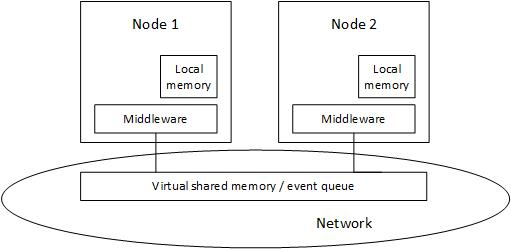
\includegraphics[width=0.8\textwidth,natwidth=610,natheight=642]{DistributedComputingSystemWith2nodes.jpg} 
	\captionsetup{format=plain,font=footnotesize,labelfont={bf,red},labelsep=quad,singlelinecheck=no}
	\caption[Distributed Computing System with 2 nodes]{
		\label{fig:distributedCoputingSystem} 
		\footnotesize{%
			A Distributed Computing System with 2 nodes.
		}
	}
\end{figure}

Figure \cref{fig:distributedCoputingSystem} illustrates the idea of a distributed computing system. Nodes 1 and 2 shares some virtual memory and/or event queue. The Middleware is a handles communication between the nodes and ensures the virtual memory is consistent throughout the network. The shared virtual memory is transparent to each node. 

Distributed systems offer many benefits over centralized systems including the following:
\begin{itemize}
	\item Scalability: It is easy to add notes to the system, should the size of the system increase.
	\item Redundancy: Several nodes can provide the same service, so if a node crashes, there are many to replace it. Additionally, from a cost perspective, each node does not have to be expensive, because many smaller nodes can be used as replacement.
\end{itemize}

\section{Thesis motivation}

\subsection{Siemens case}
Siemens Wind Power is among the leading windmill manufacturers in the world. 
Siemens builds wind farms of different sizes ranging form single mills to well above one hundred windmills \cite{simensOffShoreProjects, simensOnShoreProjects}.

In the current setup (see \cref{fig:currentSiemensSetup}) the Park Monitor is a central component and a SPOF (single point of failure).
The system is running on windows with a MSSQL database in the Park Monitor and MySQL on the windmills them self.
The windmills, Park Monitor and Park Regulator is connected with a gigabit network, witch currently has plenty of extra capacity.
The system handles more than 50 control points and 200 measurement points, and samples these every 50 ms.
The Park regulator is associated with the transformer station and regulated the power production when needed.
This component currently has a less than optimal work flow see \cref{fig:dataComputationSequence}.

Siemens has a need for their system to scale better and provide increased redundancy to avoid these SPOF's.
Siemens has a vision of removing the Park Monitor component and make it into a distributed system, distributed among the windmills (see \cref{fig:futureSiemensSetup}).
Also Siemens would like to look for ways to optimise the calculations done by the Park Regulator, 

\begin{figure}
	\centering
	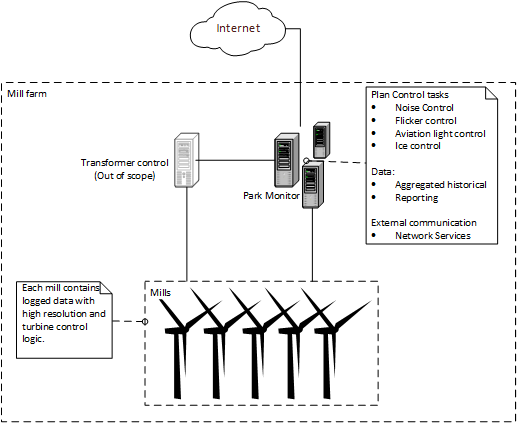
\includegraphics[width=0.7\textwidth,natwidth=610,natheight=642]{SystemOverviews.png} 
	\captionsetup{format=plain,font=footnotesize,labelfont={bf,red},labelsep=quad,singlelinecheck=no}
	\caption[Illustrates the current Siemens windmill farm setup]{
		\label{fig:currentSiemensSetup} 
		\footnotesize{%
			This figure illustrates the current Siemens windmill farm setup.
		}
	}
\end{figure}

\begin{figure}
	\centering
	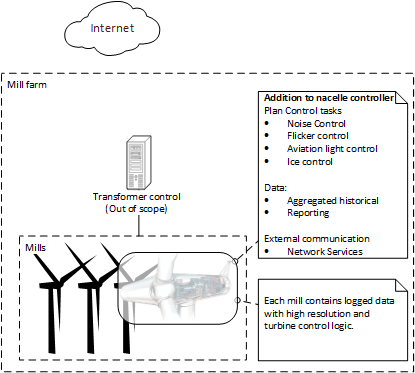
\includegraphics[width=0.7\textwidth,natwidth=610,natheight=642]{SystemOverviewsFuture.png} 
	\captionsetup{format=plain,font=footnotesize,labelfont={bf,red},labelsep=quad,singlelinecheck=no}
	\caption[Illustrates the future Siemens windmill farm setup]{
		\label{fig:futureSiemensSetup} 
		\footnotesize{%
			This figure illustrates the future Siemens windmill farm setup.
		}
	}
\end{figure}

\begin{figure}
	\centering
	\begin{sequencediagram} %Created using pgf-umlsd
		\newthread{reg}{:Park Regulartor}
		\newinst[2]{mill}{:Mill}
	
		\begin{sdblock}{each mill}{}
			\mess[1]{reg}{getCurrentStatus}{mill}
			\mess[1]{mill}{status}{reg}	
		\end{sdblock}
		
		\begin{call}{reg}{calculateAllSetpoints()}{reg}{}
		\end{call}
	
		\begin{sdblock}{each mill}{}
			\mess[1]{reg}{setNewSetpoint}{mill}
		\end{sdblock}
					
	\end{sequencediagram}

	\captionsetup{format=plain,font=footnotesize,labelfont={bf,red},labelsep=quad,singlelinecheck=no}
	\caption[Regulator calculation sequence]{
		\label{fig:dataComputationSequence} 
		\footnotesize{%
			Regulator calculation sequence.
		}
	}
\end{figure}
















\subsection{et eller andet}

Today windmills in windmill farm at Siemens are equipped with a computer for regulation, data and communication purposes. Every windmill are connected to a single server that aggregates data, perform calculations, store data and handle communication with the outside world. At Siemens up to 8 of theses servers are present pr. windmill farm and they pose the following problems:
\begin{itemize} 
	\item Single point of failure. Should a server fail, a part of the windmill farm will become unavailable.
	\item Low scalability. The servers does not scale with the number of windmills.
	\item Up performance of park regulator.
\end{itemize}

Therefor Siemens wishes to remove the servers by making every windmill farm a Distributed Computing System, utilizing free capacity of the computers already residing in every windmill. This would up the redundancy and scalability and the remove possibility of a single point of failure. A windmill farm must serve as single server which means ease of access must be maintained even though computation and data is distributed. This means routing traffic to a windmill with free capacity through a single interface, without external systems being aware of it.

% Today windmills in windmill farm are connected to a single server that aggregates data, perform calculations, store data and handle communication with the outside world. These servers do not scale well with the size of the windmill farm, and they are a single point of failure. Therefor Siemens wishes to remove the servers by utilizing free capacity of the computers already residing in every windmill. 
%Currently there is some limited redundancy in data and availability but this could be greatly improved by distributing data and communication to the windmills. 
%Ease of access must be maintained even though computation and data is distributed. 
%This means routing traffic to a windmill with free capacity through  a single interface.

\section{Thesis aim}

The purpose of this thesis is to design, implement and evaluate a framework and associated tools for distributed computing systems development. The case from Siemens Windpower is an example of a production environment where the framework could be utilized. The goal is not to make a framework that is specific to the Siemens case but to make a general framework for this and similar cases. 

This framework must be able to handle computation distributed on several nodes, communication between those nodes and distribution of data. 

The framework will be evaluated with regards to the existing Siemens solution using the following parameters: ... and will be done by comparing results obtained from a protocol 


%\begin{itemize}
%	\item How do we distribute a database and computation across a production environment in the best possible way?
%	\item How do we define and measure performance?
%	\item Can it provide data redundancy and outperform current systems?
%	\item How many windmills are needed before it makes sense to makes sense to distribute the server?
%\end{itemize}
%
%We aim to investigate the possibility of making a framework and associated tools for developing a distributed system. 
%This framework must be able to handle computation distributed on several nodes, communication between those nodes and distribution of data. 
%The communication can be built on top of existing standards as for instance DDS. Data distribution can be built using existing systems like MongoDB. 
%Distribution of computation tasks is the main research area and will be the focus of this thesis.
%
%In order to achieve distributed computation on several nodes the framework must be able to perform load balancing and control the distribution of tasks on the nodes in the system. 
%Furthermore the framework must have a single interface for control of, and interaction with, all the nodes.  
%The goal is to create a test system, that can distribute and perform tasks but also to be able to plan ahead of time and know if there is available computation time.
%
%The case from Siemens Windpower is an example of a production environment where the framework could be utilized. 
%Our goal is not to make a framework that is only  specific for this case but to make a general framework for this and similar cases.

\section{Approach}

\section{Outline}
The remainder of this thesis is organized into the following chapters...

\section{Audience}
This thesis is aimed at an audience with a basic knowledge of...

% include{dedication}
% include{RelatedWork}
\chapter{Analysis}
% include{Technologies}
\chapter{The Proposed Centralized Solution}\label{cha:existingSystem}

The \ref{PS:Q:Scalability} problem in the problem statement(\cref{sec:problemStatement}) requires a comparison between the decentralized solution and the current system at Siemens on different parameters. Ideally, for us to compare the two systems on equal terms, both systems should be implemented in the same environment. However, since we do not have access to the environment where the current system at Siemens is implemented, we have chosen to build our own version of the current Siemens system, in the same environment as the decentralized solution.

This version of the current Siemens system, from now on referred to as the centralized solution, is built from what Siemens has informed about the current Siemens system. The goal of the centralized solution is to create a foundation for a comparison between the decentralized solution and the current Siemens system, by making the system architecture around the regulation algorithm the only parameter changed from the centralized solution to the decentralized solution, thus ruling out the environment difference of the two systems as a parameter. This means the centralized solution is built to enable the collection of data that can be used to compare the two systems. As a result, we aim to compare the decentralized solutions test results with the centralized solutions test results, collected within the same environment, to more accurately address the \cref{PS:Q:Scalability} problem.

However in order to completely answer the \ref{PS:Q:Scalability} question, and compare the decentralized solution with the current Siemens system, another comparison must be introduced: A comparison between our centralized solution and the current Siemens system. This comparison is relevant in order to close the remaining 'comparison-gap' between the decentralized solution and the current Siemens system. This comparison will be a theoretical comparison between the centralized solution and the current Siemens system, and based on assumptions made when building the centralized solution.

As presented in \cref{fig:projectDiffOverview} there exist a difference between the current Siemens system and the centralized solution as well as a difference between the centralized solution and the decentralized solution, illustrated by deltas.

\begin{figure}[!h]
	\centering
	\begin{tikzpicture}[
	node distance = 0.3cm,
	auto,
	block/.style={draw, rectangle, text width=5em, text centered, minimum height=5cm}		
	]
% Place nodes
\node [block]			(Siemens)												[label=above:Siemens system]	{};
\node []					(SimCen)		[right = of Siemens] 	{$\Delta$};
\node [block]			(OurCent)		[right = of SimCen] 	[label=above:Centralized solution]	{};

\begin{scope}[on background layer]
\node [block] 		(Central) 	[fit=(Siemens) (OurCent), inner sep=20pt] {};
\node []					(CenDece)		[right = of Central] 	{$\Delta$};
\node [block]			(DeCent)		[right = of CenDece] 	[label=above:Decentralized solution] {};
\end{scope}

\end{tikzpicture}
	\captionsetup{format=plain,font=footnotesize,labelfont={bf,defaultCapFont},labelsep=quad,singlelinecheck=no}
	\caption[Comparison overview]{
		\label{fig:projectDiffOverview} 
		\footnotesize{%
			Comparison overview.
		}
	}
\end{figure}

The delta between the current Siemens system and the centralized solution is minimized as much as possible based on information about the current Siemens system delivered by Siemens Wind Power. Since the operation and regulation of the current Siemens system is proprietary the full system information is not available. To make up for the missing information a number of assumptions has been done about the current Siemens system which is also a part of the delta.
The delta between the centralized solution and decentralized solution describes the difference in operation of a centralized system and a decentralized system.

The thesis motivation (\cref{sec:ThesisMotivation}) describes a brief overview of the current system at Siemens. This chapter gives a detailed description of the key component of the current Siemens system: The regulation algorithm. Furthermore the chapter describes the centralized solution followed by a theoretical comparison between the centralized solution and the current Siemens system. 

\section{Regulation algorithm}\label{sec:cenRegAlgorithm}

The regulation algorithm is a key component of the current Siemens system and it is where new setpoints are calculated. Since the purpose of this thesis is not to improve any regulation algorithms, the regulation algorithm has been considered a black box in development of both the centralized and the decentralized solution. What is important to this thesis is that the algorithm used is the same in both the centralized and the decentralized solution, to make sure the two solutions are compared on the same terms. 

%To get as realistic a picture of the system as possible of the regulation algorithm, we tried to gain access to the algorithm Siemens currently use, but due to the regulation algorithm at Siemens being a commercial secret, this was not possible.

\begin{figure}
	\centering
	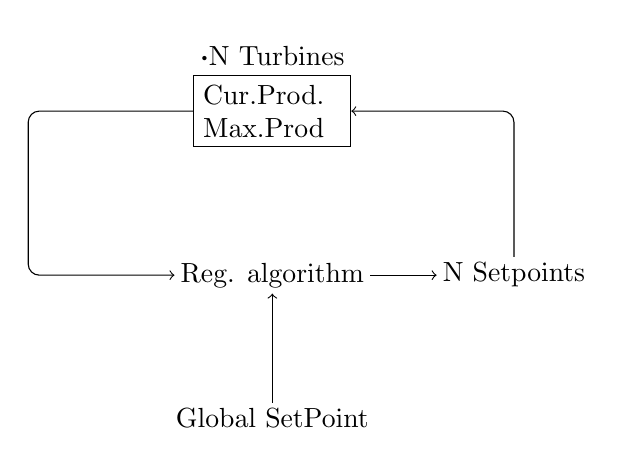
\begin{tikzpicture}[
	point/.style={inner sep=0pt}, %circle,minimum size=2pt,fill=red},
	textNode/.style={inner sep=2pt},
	hv path/.style={to path={-| (\tikztotarget)}},
	vh path/.style={to path={|- (\tikztotarget)}},
	skip loop h/.style={to path={-- ++(0,#1) -| (\tikztotarget)}},
	skip loop v/.style={to path={-- ++(#1,0) |- (\tikztotarget)}},
	graphs/every graph/.style={edges=rounded corners}
	]
	
% Place nodes
\matrix[row sep=1.4cm,column sep=.4cm] {
	\node [point]  		(p1x1)	{}; &&
	\node [rectangle]	(Turbine)		[draw, label=above:\textbf{$\cdot$}N Turbines, text width=50pt]	{Cur.Prod. Max.Prod}; &&
	\node [point]  		(p1x3)	{}; \\
	
	\node [point]  		(p2x1)			{}; &&
	\node [textNode]	(HPPP)		 	{Reg. algorithm}; &&
	\node [textNode]	(Setpoint)	{N Setpoints}; \\

	&& \node [textNode]  (gSetpoint)							{Global SetPoint}; \\
};
	
\graph[use existing nodes]{
	Turbine ->[skip loop v=-3.1cm] HPPP -> Setpoint ->[vh path] Turbine;
	gSetpoint -> HPPP;
};

\end{tikzpicture}



%\begin{tikzpicture}[
%	point/.style={inner sep=0pt}, %circle,minimum size=2pt,fill=red},
%	textNode/.style={inner sep=2pt},
%	hv path/.style={to path={-| (\tikztotarget)}},
%	vh path/.style={to path={|- (\tikztotarget)}},
%	skip loop h/.style={to path={-- ++(0,#1) -| (\tikztotarget)}},
%	skip loop v/.style={to path={-- ++(#1,0) |- (\tikztotarget)}},
%	graphs/every graph/.style={edges=rounded corners}
%	]
%	
%% Place nodes
%\matrix[row sep=1.5cm,column sep=.5cm] {
%	\node [point]  		(p1x1)	{}; &&
%	\node [rectangle]	(Turbine)		[draw, label=above:\textbf{$\cdot$}N Turbines, text width=50pt]	{Cur.Prod. Max.Prod}; &&
%	\node [point]  		(p1x3)	{}; \\
%	
%	\node [point]  		(p2x1)			{}; &&
%	\node [textNode]	(HPPP)		 	{HPPP}; &&
%	\node [textNode]	(Setpoint)	{\textbf{$\cdot$}N Setpoints}; \\
%
%	\node [textNode]  (gSetpoint)										{Global SetPoint}; &&
%	\node [rectangle]	(Data)			[draw, text width=50pt] {Cur.prod  Max.Prod};\\
%};
%
%\node [textNode,right of=Data] {~~~~~~~~~~~~~~~~~\textbf{$\cdot$}N Turbines};
%	
%\graph[use existing nodes]{
%	Turbine ->[skip loop v=-2.7cm] HPPP -> Setpoint ->[vh path] Turbine;
%	gSetpoint.east -> HPPP;
%	Data -> HPPP;
%};
%
%\end{tikzpicture}

	\captionsetup{format=plain,font=footnotesize,labelfont={bf,defaultCapFont},labelsep=quad,singlelinecheck=no}
	\caption[Centralized input/output parameters of the regulation algorithm]{
		\label{fig:ioCenRegAlg} 
		\footnotesize{%
			Centralized input/output parameters of the regulation algorithm.
		}
	}
\end{figure}

With the algorithm being a black box, the input/output parameters of the regulation algorithm was studied to provide the correct communication circumstances for the regulation algorithm. \Cref{fig:ioCenRegAlg} presents a simple input/output overview of the regulation algorithm. Input/output parameters of the regulation algorithm are as follows:

\begin{description}
	\item The \textbf{global setpoint} of the wind farm. This is the production goal of the wind farm. %Which means all turbines combined should produce.
	\item The \textbf{setpoint} of each turbine, calculated from the regulation algorithm. 
	\item The \textbf{current production} of the turbine.
	\item The \textbf{maximum production} of the turbine. In real-life, this parameter is amongst others determined from the wind conditions around the turbine.
\end{description}

These input/output parameters of the regulation algorithm is simplified compared to the current Siemens system. The data used is more og less irrelevant for the purpose of this thesis as long as both the decentralized solution and the centralized solution are using the same data and as long as both systems are able to perform the same simple regulation.

\section{Regulation cycle}\label{sec:currentSystemCen} 

The first area studied when building the centralized solution, was building the frames for the regulation algorithm (see \cref{sec:cenRegAlgorithm}), meaning how to communicate the input/output around the centralized solution.

This section describes the components of a regulation cycle in the centralized solution. The regulation cycle consist of a number of steps presented in \cref{fig:timingCentral}.

\begin{figure}[!h]
	%The figure show how regulation time differs central vs decantral
	

{ %The brackets issolate the enviroment

\tikzstyle{line}		 	= [draw]

\makeatletter
\ifcsname c@wavenum\endcsname %Only create one counter
\else
	\newcounter{wavenum}
\fi
\makeatother

\newcommand*{\bitvector}[3]{
  \draw[fill=#3] (t_cur) -- ++( .1, .3) -- ++(#2-.2,0) -- ++(.1, -.3)
                         -- ++(-.1,-.3) -- ++(.2-#2,0) -- cycle;
  \path (t_cur) -- node[anchor=mid](textNode) {#1} ++(#2,0) node[time] (t_cur) {};
  }

% \known{val}{length}
\newcommand*{\known}[2]{
    \bitvector{#1}{#2}{white}
}

% \unknown{length}
\newcommand*{\unknown}[2]{
    \bitvector{#1}{#2}{black!20}
}

% \nextwave{name}
\newcommand{\nextwave}[1]{
  %\path (0,\value{wavenum}) node[time] (t_cur) {};
   \path (0,\value{wavenum}) node[left] {#1} node[time] (t_cur) {};
  \addtocounter{wavenum}{-1}
}

\newcommand{\timeSpanLabel}{
	\node (CycleTimeLabel) [rectangle, above = 0.7cm of textNode, inner sep=0pt] {Regulation cycle time};	  
}

\newcommand{\timeSpanA}{
	\node (t_timeSpanA) [point, above = 0 of t_cur] {};	  
}

\newcommand{\timeSpanB}{
	\node (t_timeSpanB) [point, above =0 of t_cur] {};

  \graph[use existing nodes]{
  	t_timeSpanA --[time span=1cm] CycleTimeLabel;
   	CycleTimeLabel.south --[time span=-0.24cm] t_timeSpanB;
  }; 
    	
}


%%% End of timing.sty
\begin{tikzpicture}[
	point/.style={inner sep=0pt}, %circle,minimum size=2pt,fill=red},
	draw=black, 
	yscale=.8,
	xscale=1,
	hv path/.style={to path={-| (\tikztotarget)}},
	vh path/.style={to path={|- (\tikztotarget)}},
	skip loop v/.style={to path={-- ++(#1,0) |- (\tikztotarget)}},		
	skip loop h/.style={to path={-- ++(0,#1) -| (\tikztotarget)}},
	time span/.style={to path={-- ++(0,#1) -| (\tikztotarget)}},
	graphs/every graph/.style={edges=rounded corners}	
	]
	
  \tikzstyle{time}=[coordinate]
  \setlength{\unitlength}{1cm}
  \setcounter{wavenum}{0}
    
  %\nextwave{Regulation Time} \unknown{SendData}{2} \known{WaitForData}{5} \unknown{ReciveData}{2} \unknown{Calculate}{2}\unknown{SendSP}{2}
  \nextwave{Park Pilot} \unknown{reqStates}{1.8} \known{wait}{2} \unknown{readStates}{2} \unknown{regAlg.}{1.7} \unknown{sendSetpoints}{2.6}
  
  \nextwave{Turbine} \known{wait}{1.8} \unknown{replyState}{2} \known{wait}{6.3} \unknown{receiveSetpoint}{2.9}
    
  
\end{tikzpicture}
}

	\caption{The regulation cycle of the centralized solution}
	\label{fig:timingCentral}
\end{figure}

\subsection{Get turbine states}\label{sec:getTurbineStates}

In order for the Park Pilot to calculate turbine setpoints, the Park Pilot must have the state of all turbines.

\begin{figure}
	\centering
	\begin{sequencediagram} %Created using pgf-umlsd
		\newthread{parkPilot}{:Park Pilot}
		\newthread{turbineDataReplier}{:Turbine Data Replier}
		\newinst{turbine}{:Turbine}
	
		\begin{sdblock}{each turbine}{}
			\mess[1]{parkPilot}{reqState}{turbineDataReplier}
			\begin {call}{turbineDataReplier}{readState()}{turbine}{return state}
			\end {call}
			\mess[1]{turbineDataReplier}{replyState}{parkPilot}
		\end{sdblock}				
	\end{sequencediagram}

	\captionsetup{format=plain,font=footnotesize,labelfont={bf,defaultCapFont},labelsep=quad,singlelinecheck=no}
	\caption[First part of the regulation cycle]{
		\label{fig:getStatesOfTurbines} 
		\footnotesize{%
			First part of the regulation cycle: Getting the state of all turbines.
		}
	}
\end{figure}

A simple overview of the first part of the regulation cycle is presented on \cref{fig:getStatesOfTurbines}. This part of the regulation cycle is implemented using the RTI Connext Request-Reply implementation~\cite{rtiConnextUsersManual}. The three primary objects of this part of the regulation cycle are:

\begin{description}
	\item [Park Pilot] The Park Pilot requests the current state of all turbines and calculates setpoints when states has been received.
	\item [Turbine Data Replier] The replier object handles the request and sends a reply.
	\item [Turbine] The underlying turbine object is the interface to the Turbine, which handles communication with the underlying database with simulation data.
\end{description}

The Park Pilot sends a request to a specific DDS Topic and then waits until it has received a reply from all the turbines subscribing to this DDS Topic, which in our case is all turbines. In a real-life implementation of the centralized solution, a timer should be implemented to determine how long to wait for the replies, and maybe even mark a turbine as offline, if a given turbine does not reply within that time frame. However, since this is a prototype for comparison purposes, this functionality has not been implemented. The request message, sent from the Park Pilot, contains the regulation cycle time, which is only used for data logging purposes (i.e. not used by the turbines).

The Turbine Data Replier is instantiated with the Turbine object and runs on every turbine. After instantiation, the Turbine Data Replier goes into an infinite loop which first waits infinitely until a request is received, reads turbine data from the Turbine object and finally sends a reply containing the data to the Park Pilot. Ideally, the Turbine Data Replier object should have been implemented as a listener on the request topic using RTI Connext SimpleReplier~\cite{rtiConnextUsersManual}. However, we could not get it to work using the SimpleReplier but waiting infinitely for a request works just as well for our purpose.

The Turbine object is the interface to the actual Turbine. The primary functionality of this object is to change state when a new setpoint is assigned to the object. Furthermore it reads data from the underlying MongoDB database. 

\subsection{Calculate setpoints (regAlgorithm)}\label{sec:calculateSetpoints}

When the Park Pilot has received the states of all turbines the setpoints for all turbines are calculated. Since we don't have access to Siemens' regulation algorithm (see \cref{sec:cenRegAlgorithm} for explanation), we have developed our own simple regulation algorithm. The code for this regulation algorithm is presented on \cref{fig:cenRegAlgCode}.

\begin{figure}[!h]
	\centering
%	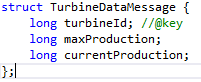
\includegraphics[width=0.3\textwidth,natwidth=250,natheight=200]{turbineDataMessage.PNG} 
	\begin{lstlisting}[language=C++,tabsize=2,basicstyle=\small]
void CentralizedParkPilot::regAlgorithm(
	uint_fast32_t globalSetpoint,
	LoanedSamples<TurbineDataMessage> &turbines)
{
	int availableTurbinesCount = turbines.length();

	typedef LoanedSamples<TurbineDataMessage>::iterator iterator;
	long localSetpoint = 0;

	for (iterator it = turbines.begin(); it != turbines.end(); ++it) {
		if (it->info().valid_data) {

			if (it->data().currentProduction >= it->data().maxProduction) {
				availableTurbinesCount--;
			}
		}
		else
			availableTurbinesCount--;
	}

	for (iterator it = turbines.begin(); it != turbines.end(); ++it) {
		if (it->info().valid_data) {
			if (availableTurbinesCount <= 0)
				localSetpoint = globalSetpoint;
			else
				localSetpoint = globalSetpoint / availableTurbinesCount;

			if (localSetpoint > it->data().maxProduction) {
				localSetpoint = it->data().maxProduction;
			}

			_turbineOutlets[it->data().turbineId - START_ID]->
						setSetpoint(localSetpoint);
					
			_turbineOutlets[it->data().turbineId - START_ID]->publishData();
		}
	}
}
	\end{lstlisting}
	\captionsetup{format=plain,font=footnotesize,labelfont={bf,defaultCapFont},labelsep=quad,singlelinecheck=no}
	\caption[The regulation algorithm of the centralized solution]{
		\label{fig:cenRegAlgCode} 
		\footnotesize{%
			Code for the centralized regulation algorithm used to calculate setpoints.
		}
	}
\end{figure}


Our regulation algorithm works by first determining how many turbines that are available for production. This is done going through every turbine, checking if they currently hit their maximum production capacity. If a given turbine is producing at maximum capacity, a greater load cannot be assigned to it and the available turbine count is reduced. 

Next the setpoint for every turbine is calculated using this simple formula: $setpoint=globalSetpoint/availableTurbines$. If this new setpoint is higher than the maximum capacity of a given turbine, the turbine is set to produce at maximum capacity. If this happens, a gap between the maximum capacity and the calculated setpoint is left unhandled, and the wind farm is under-producing until the next cycle, where a new set of setpoints are calculated, with one less available turbine. Hence this gap will eventually be closed unless the maximum capacity of the entire park is reached.

\subsection{Send setpoints}

\Cref{fig:sendSetpoints} presents a simple overview of the last part of the regulation cycle. This part of the regulation cycle is implemented using RTI Connext Publish-Subscribe implementation~\cite{rtiConnextUsersManual}. The primary objects are:

\begin{description}
	\item [Park Pilot] Explained in \cref{sec:getTurbineStates}.
	\item [Turbine Outlet] The Park Pilots implementation of a given turbine. One Turbine Outlet is instantiated on the Park Pilot for each turbine in the park. Writing data to each turbine is handled from this object.
	\item [Setpoint Listener] The listener object called when when a new setpoint is published. One Setpoint Listener are instantiated on each turbine.
	\item [Turbine] Explained in \cref{sec:getTurbineStates}.
\end{description}

After calculating the setpoints (\cref{sec:calculateSetpoints}), the Park Pilot sends a new setpoint to each turbine. The Park Pilot sets the setpoint of the Turbine Outlet before publishing the Data.

\begin{figure}[!h]
	\centering
	\begin{sequencediagram} %Created using pgf-umlsd
		\newthread{parkPilot}{:Park Pilot}
		\newinst{turbineOutlet}{:Turbine Outlet}
		\newinst{setPointListener}{:Setpoint Listener}
		\newinst{turbine}{:Turbine}
	
		\begin{sdblock}{each turbineOutlet}{}
			\begin {call}{parkPilot}{setSetpoint()}{turbineOutlet}{}
			\end {call}
			\begin {call}{parkPilot}{publishData()}{turbineOutlet}{}
				\mess[1]{turbineOutlet}{write}{setPointListener}
				\begin {call}{setPointListener}{setSetpoint()}{turbine}{}
				\end {call}
			\end {call}
		\end{sdblock}				
	\end{sequencediagram}

	\captionsetup{format=plain,font=footnotesize,labelfont={bf,defaultCapFont},labelsep=quad,singlelinecheck=no}
	\caption[Last part of the regulation cycle]{
		\label{fig:sendSetpoints} 
		\footnotesize{%
			Last part of the regulation sequence: Sending setpoints to all turbines.
		}
	}
\end{figure}

The main purpose of Turbine Outlet object is to register and publish setpoints to each turbine. Upon instantiation, the Turbine Outlet registers the turbine id as a RTI Connext key~\cite{rtiConnextUsersManual} to the setpoint topic and saves the handle object. Saving the handle upon registration and using the handle when writing improves performance~\cite{DDSInstanceHandlet}, which is why the handle is saved with the object. Lastly the object writes the data to the topic.

The Setpoint Listener object is a listener on the setpoint topic. The setpoint topic is configured with as a Content Filtered Topic~\cite{rtiConnextUsersManual}, so the listener only reacts to messages with a key that equals the turbines id (see \cref{sec:ddsConfigCen} for DDS configuration). When Setpoint Listener object is invoked, the new setpoint is saved to the Turbine object, which updates the state of the turbine.

\section{DDS configuration}\label{sec:ddsConfigCen} 

The key component used for communication is DDS (see \cref{sec:DSM}). This section describes how DDS has been configured for the centralized solution.

\subsection{Interface Description Language}\label{sec:cenIdl}

The data transfer objects (DTO) used when sending messages from the turbines to the Park Pilot, and the other way around, is created using the RTI Connext Interface Description Language~\cite{rtiConnextUsersManual}. DTOs are defined in an IDL file (see \cref{fig:cenTurbineDataMessage} for IDL example). From there the actual implementations of the IDL definitions are auto generated from the command prompt using the \textit{rtiddsgen}~\cite{rtiConnextUsersManual} command.

\begin{figure}[!h]
	\centering
%	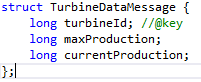
\includegraphics[width=0.3\textwidth,natwidth=250,natheight=200]{turbineDataMessage.PNG} 
	\begin{lstlisting}[language=C++,tabsize=2,basicstyle=\small]
	struct TurbineDataMessage {
		long turbineId; //@key
		long maxProduction;
		long currentProduction;	
	}	
	\end{lstlisting}
	\captionsetup{format=plain,font=footnotesize,labelfont={bf,defaultCapFont},labelsep=quad,singlelinecheck=no}
	\caption[Centralized turbine reply message]{
		\label{fig:cenTurbineDataMessage} 
		\footnotesize{%
			The the reply message .idl file sent from the turbines to the Park Pilot in the centralized solution.
		}
	}
\end{figure}

The IDL definitions are defined from looking at what data to transfer between the turbines and the Park Pilot. \Cref{fig:cenTurbineDataMessage} is for example the IDL definition of the data transfer object used as reply from the turbines to the Park Pilot.

%\subsection{Topics}
%
%Including the topics generated from the RTI Connext Request-Reply implementation~\cite{rtiConnextUsersManual} the following topics are used:
%
%\begin{figure}
%	\centering
%	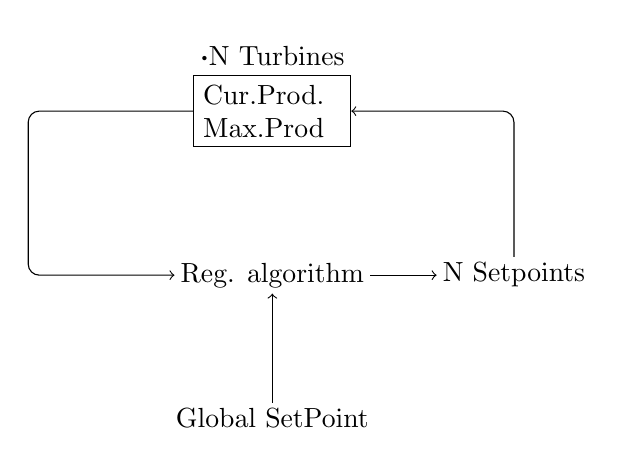
\begin{tikzpicture}[
	point/.style={inner sep=0pt}, %circle,minimum size=2pt,fill=red},
	textNode/.style={inner sep=2pt},
	hv path/.style={to path={-| (\tikztotarget)}},
	vh path/.style={to path={|- (\tikztotarget)}},
	skip loop h/.style={to path={-- ++(0,#1) -| (\tikztotarget)}},
	skip loop v/.style={to path={-- ++(#1,0) |- (\tikztotarget)}},
	graphs/every graph/.style={edges=rounded corners}
	]
	
% Place nodes
\matrix[row sep=1.4cm,column sep=.4cm] {
	\node [point]  		(p1x1)	{}; &&
	\node [rectangle]	(Turbine)		[draw, label=above:\textbf{$\cdot$}N Turbines, text width=50pt]	{Cur.Prod. Max.Prod}; &&
	\node [point]  		(p1x3)	{}; \\
	
	\node [point]  		(p2x1)			{}; &&
	\node [textNode]	(HPPP)		 	{Reg. algorithm}; &&
	\node [textNode]	(Setpoint)	{N Setpoints}; \\

	&& \node [textNode]  (gSetpoint)							{Global SetPoint}; \\
};
	
\graph[use existing nodes]{
	Turbine ->[skip loop v=-3.1cm] HPPP -> Setpoint ->[vh path] Turbine;
	gSetpoint -> HPPP;
};

\end{tikzpicture}



%\begin{tikzpicture}[
%	point/.style={inner sep=0pt}, %circle,minimum size=2pt,fill=red},
%	textNode/.style={inner sep=2pt},
%	hv path/.style={to path={-| (\tikztotarget)}},
%	vh path/.style={to path={|- (\tikztotarget)}},
%	skip loop h/.style={to path={-- ++(0,#1) -| (\tikztotarget)}},
%	skip loop v/.style={to path={-- ++(#1,0) |- (\tikztotarget)}},
%	graphs/every graph/.style={edges=rounded corners}
%	]
%	
%% Place nodes
%\matrix[row sep=1.5cm,column sep=.5cm] {
%	\node [point]  		(p1x1)	{}; &&
%	\node [rectangle]	(Turbine)		[draw, label=above:\textbf{$\cdot$}N Turbines, text width=50pt]	{Cur.Prod. Max.Prod}; &&
%	\node [point]  		(p1x3)	{}; \\
%	
%	\node [point]  		(p2x1)			{}; &&
%	\node [textNode]	(HPPP)		 	{HPPP}; &&
%	\node [textNode]	(Setpoint)	{\textbf{$\cdot$}N Setpoints}; \\
%
%	\node [textNode]  (gSetpoint)										{Global SetPoint}; &&
%	\node [rectangle]	(Data)			[draw, text width=50pt] {Cur.prod  Max.Prod};\\
%};
%
%\node [textNode,right of=Data] {~~~~~~~~~~~~~~~~~\textbf{$\cdot$}N Turbines};
%	
%\graph[use existing nodes]{
%	Turbine ->[skip loop v=-2.7cm] HPPP -> Setpoint ->[vh path] Turbine;
%	gSetpoint.east -> HPPP;
%	Data -> HPPP;
%};
%
%\end{tikzpicture}
%
%	\captionsetup{format=plain,font=footnotesize,labelfont={bf,defaultCapFont},labelsep=quad,singlelinecheck=no}
%	\caption[Regulation aslgorithm input/output parameters]{
%		\label{fig:ioRegAlg} 
%		\footnotesize{%
%			Input/output parameters of the regulation algorithm.
%		}
%	}
%\end{figure}

\subsection{Choosing quality of service parameters}\label{sec:choosingQosParams}

Quality of Service (QoS) parameters are parameters used to determine the behavior of a system using RTI Connext DDS. As such, setting the right QoS parameters for the centralized solution is important in order to duplicate the behavior of the current system at Siemens as close as possible. 

In order to decide the QoS parameters for the centralized solution, the QoS XML file from the current system at Siemens was provided by Siemens (see \cref{appendix:siemensQosFile} for the QoS XML file). Thus QoS parameters for the centralized solution has been set using this file, which presents many different QoS profiles.

The Siemens QoS XML file specifies one \textit{DomainParticipantFactory} profile. This profile has been applied to the solution and parameters irrelevant to the purpose of this thesis has been removed from the profile. 

The Siemens QoS XML file specifies two \textit{DomainParticipant} profiles. One using UDPv4 and one using DTLS as transport plugin. The one using UDPv4 has been chosen for the centralized solution, since DTLS encryption and decryption is an unnecessary overhead, that either should be introduced to both the centralized- and the decentralized solution or to neither, for the two solutions to be compared on the same terms. Thus for simplicity neither of the solutions introduce DTLS.

As for \textit{DataReaders}, \textit{DataWriters} and \textit{Topics}, the file specifies multiple profiles the use of which is unknown. Thus it is unknown which ones has been used for the part of the system that is implemented with the centralized solution. Furthermore since the centralized solution is a simplified version of the current Siemens system it will not need the number of \textit{DataReaders}, \textit{DataWriters} and \textit{Topics} that the current Siemens system apply.

Each Qos parameter in every QoS profile has been evaluated and the parameters relevant to the purpose of this theses has been applied to the centralized solution, based on assumptions about the current Siemens system. The QoS XML file roughly presents profiles that combines the following parameters in different ways:

\paragraph{Reliability} is the QoS parameter, which determines whether or not data published by a \textit{DataWriter} will be reliably delivered by the DDS framework to matching \textit{DataReaders}~\cite{rtiConnextUsersManual}. The three levels of reliability presented by the different profiles are:

\begin{itemize}
	\item \textbf{Best effort reliability} profiles are configured so data samples are sent once and missed samples are acceptable.
	\item \textbf{Reliable} profiles are configured to make sure that data sent is received and missed samples are resent. \textit{DataWriters} will send samples reliably to \textit{DataReaders}, buffering sent data until they have been acknowledged as being received by \textit{DataReaders} and resending any samples that may have been lost during transport. The \textit{DataWriter} buffer of this configuration is set to the size of one message, which means only the newest message is resent. This implies that an unacknowledged sample may be overwritten and thus lost. 
	\item \textbf{Strictly reliable} profiles are configured like reliable profiles, but with a larger \textit{DataWriter} buffer. Increasing the \textit{DataWriter} buffer size will decrease the chance of unacknowledged samples being overwritten. Thus \textit{DataReaders} are ensured all messages sent by the \textit{DataWriters}.
\end{itemize}

\paragraph{Durability} controls whether or not, and how, published samples are stored by the \textit{DataWriter} application for \textit{DataReaders} that are found after the samples were initially written, thus allowing new \textit{DataReaders} to receive data sent before they were created. The levels of durability presented by the different profiles are:

\begin{itemize}
	\item \textbf{No durability} profiles are configured not to store any samples for newly discovered \textit{DataReaders}.
	\item \textbf{Local durability} profiles are configured such that \textit{DataWriters} will store and send previously published samples for delivery to newly discovered \textit{DataReaders} as long as the \textit{DataWriter} still exists.
\end{itemize}

\paragraph{Throughput} is configured using the batch~\cite{rtiConnextUsersManual} parameter, which can be used to decrease the amount of communication overhead associated with the transmission and (in case of reliable communication) acknowledgment of small samples at the expense of latency. This is done by batching many smaller samples to be sent in a single large packet, which increases network utilization and thus throughput in terms of samples per second. The two levels of throughput presented by the different profiles are:

\begin{itemize}
	\item \textbf{Regular throughout} profiles are configured to avoid batching of samples, thus data samples and (in case of reliable communication) acknowledgment message are sent individually.
	\item \textbf{High throughput} profiles are configured such that \textit{DataWriters} will batch data in order to increase throughput.
\end{itemize}

The many profiles in the Siemens QoS XML file (\cref{appendix:siemensQosFile}) are presumably made for many different purposes. For building the centralized solution, the profile using \textbf{Strictly reliable}, \textbf{No durability} and \textbf{Regular throughput} configurations was chosen based on the following assumptions about the current Siemens system:

\begin{itemize}
	\item \textbf{Strictly reliable} messaging is important for the Park Pilot to compute setpoints for each turbine, since states of all turbines are needed in order to calculate setpoints. Thus resending a sample data if the sample data is dropped is needed in order to calculate setpoints. 
	\item \textbf{No durability} is needed for the regulation algorithm. If a new turbine is discovered, the turbine have no need of receiving old requests or setpoints. The turbine only needs to make itself available to requests from the Park Pilot and thereby be taken into account, which is done automatically by \textit{Connext} when a the new \textit{DataReader} of the turbine is discovered.  
	\item \textbf{Regular throughput} provides the best performance for the regulation cycle. Batching data samples does not make any sense for the centralized solution since during the regulation cycle, a given node can only fall one message behind and since heartbeats and data samples are batched per default.
\end{itemize}

The chosen profile from the current Siemens system QoS XML, from which QoS profiles for the centralized solution has been built, is the profile called \textit{SwpStrictReliableNoDurability} (\cref{appendix:siemensQosFile}).


\subsection{Detailed quality of service evaluation} \label{sec:detailedQoSDesc}

The section provides a detailed evaluation of every parameter of the chosen profiles of the centralized solution QoS XML file, including the QoS parameters deemed irrelevant and thereby removed from the QoS file provided by Siemens (\cref{appendix:siemensQosFile}). See \cref{appendix:centralizedQosFile} for centralized solution QoS XML file. Removed parameters are marked with '(removed)' and commented out in the figures.

\paragraph{Participant factory} (\cref{fig:parFacQos}) QoS parameters has been evaluated as follows:

\begin{itemize}
	\item \textbf{autoenable\_created\_entities (removed)} determines whether or not participants should be enabled upon initialization. For the centralized solution the default value (enabled) for this parameter is sufficient.
	\item \textbf{logging} is set for all participants and occurs on both errors and warning messages concerning the underlying platform (hardware or OS) on which \textit{RTI Connext} is running. A warning indicates that \textit{RTI Connext} is taking an action that may not be what was originally intended. This parameter is set since the current Siemens system uses this setting and for debugging purposes.
\end{itemize}

\begin{figure}
\begin{lstlisting}[language=XML]
<participant_factory_qos>
	<!--entity_factory>
		<autoenable_created_entities>false</autoenable_created_entities>
	</entity_factory-->
	<logging>
		<verbosity>WARNING</verbosity>
		<category>PLATFORM</category>
		<print_format>VERBOSE_TIMESTAMPED</print_format>
		<output_file>ddsadaptor.log</output_file>
	</logging>
</participant_factory_qos>
\end{lstlisting}
\caption[Participant factory QoS parameters]{
		\label{fig:parFacQos} 
		\footnotesize{Participant factory QoS parameters.}
	}
\end{figure}

\paragraph{Participant} (\cref{fig:parQos}) QoS parameters has been evaluated as follows:
 
\begin{itemize}
	\item \textbf{database} configures how \textit{RTI Connext} manages its internal database, which stores information about entities created locally as well as remote entities found during the discovery process. Database thread has been set to wake up and delete removed records 1 ns after a given domain participant is destroyed for cleanup purposes.
	
	\item \textbf{transport\_builtin} configures the built-in transport plugins (UDPv4/IP, UDPv6/IP, TCP/IP, TLS, DTLS, shared memory, etc.) used by the \textit{DomainParticipants}. By default UDPv4 and shared memory plugins are enabled. For the centralized solution, the shared memory plugin is disabled (set to UDPv4 only) such that applications running on the same node do not use shared memory to communicate. This is done since our test setup only involves 3 test machines, each simulating a number of turbines. As such, communication through shared memory is not acceptable, because the turbines must communicate as if they are separate machines.
	
	\item \textbf{receiver\_pool (removed)} configures the internal \textit{Connext} thread used to process the data received from a transport. As such, the \textbf{buffer\_size} configures the size of the receive buffer in bytes. The default value of this property is set to the largest message size of all installed transports, which is needed for the centralized solution. Thus the default value is sufficient and the custom value used in the current Siemens system is removed from the centralized solutions QoS file.
	
	\item \textbf{ignore\_nonup\_interfaces (removed)} property allows/disallows the use of interfaces that are not reported as UP (by the operating system) in the UDPv4 transport. Setting this value to 0 supports the communication scenarios in which interfaces are enabled after the participant is created. This parameter has been removed since the centralized solution do not have any interfaces that are enabled after the participant is created. Thus the centralized solution uses the default value of 1 which means interfaces that are reported as down is not supported.
	
	\item \textbf{multicast\_enabled (removed)} parameter is used to configure if the transport plugin (in this case UDPv4) should use multicast for sending and receiving. By removing this parameter the default value is used, which allows multicast on all network interfaces allowed for multicast that is found up and running when the plugin is instantiated. The centralized solution is \textbf{not} supposed to use multicast for sending and receiving data used in context of the regulation cycle, however multicast is acceptable for discovery of \textit{DomainParticipants}. Thus this parameter is set to default for discovery purposes.
	
	Note that we have not set any multicast addresses on the \textit{DataReader} QoS profile (see \textit{DataReader} QoS parameters later in this section), which means multicast is not used for sending and receiving data in the context of the regulation cycle.
	
	\item \textbf{message\_size\_max} configures the maximum size of a message in bytes. This value must be set before the transport plugin is registered, such that \textit{Connext} can properly use the plugin. For the purpose of the centralized solution this value is more or less irrelevant, since it's only a max value. The value of this parameter just have to be larger than the largest message size in bytes plus any overhead (ie. $message\_size\_max \geq largest\_msg + msg\_overhead$). The largest message of the centralized solution contains $3\cdot64bit=192bit$. Thus to maintain similarity to the current Siemens system and since any larger value has no influence on our test results, the value of this parameter is left as the value used by the current Siemens system at a size of 65535 bytes.
	
	\item \textbf{send\_socket\_buffer\_size} configures the size of the send buffer in bytes. This value must be greater than or equal to the value of the \textit{message\_size\_max} parameter. For the purpose of the centralized solution this value have to be big enough to contain enough messages to cover the \textit{DataWriter} history QoS (see DataWriter QoS history parameter later in this section), with regards to the largest centralized message size of $3\cdot64bit=192bits$ plus any message overhead. Thus a value of 65535 bytes is more than enough, and the value is kept to maintain similarity to the current Siemens system.
	
	\item \textbf{recv\_socket\_buffer\_size} configures the size of the receive buffer. This value must be greater than or equal to the value of the \textit{message\_size\_max} parameter. For the purpose of the centralized solution this value have to be big enough to contain enough messages to cover \textit{DataReader} history QoS (see DataReader QoS history parameter later in this section) with regards to the largest centralized message size of $3\cdot64bit=192bits$ plus any message overhead. 
\end{itemize}

\begin{figure}
\begin{lstlisting}[language=XML]
<participant_qos>
	<database>
		<shutdown_cleanup_period>
			<sec>DURATION_ZERO_SEC</sec>
			<nanosec>1</nanosec>
		</shutdown_cleanup_period>
	</database>
	<participant_name>
		<name>Siemens Wind Power DDS Adaptor</name>
	</participant_name>
	<transport_builtin>
		<mask>UDPv4</mask>
	</transport_builtin>
	<!--receiver_pool>
		<buffer_size>65535</buffer_size>
	</receiver_pool-->
	<property>
		<value>
			<!--element>
				<name>dds.transport.UDPv4.builtin.ignore_nonup_interfaces</name>
				<value>0</value>
			</element>
			<element>
				<name>dds.transport.UDPv4.builtin.multicast_enabled</name>
				<value>0</value>
			</element-->
			<element>
				<name>dds.transport.UDPv4.builtin.parent.message_size_max</name>
				<value>65535</value>
			</element>
			<element>
				<name>dds.transport.UDPv4.builtin.send_socket_buffer_size</name>
				<value>65535</value>
			</element>
			<element>
				<name>dds.transport.UDPv4.builtin.recv_socket_buffer_size</name>
				<value>2097152</value>
			</element>
		</value>
	</property>
</participant_qos>
\end{lstlisting}
\caption[Participant QoS parameters]{
		\label{fig:parQos} 
		\footnotesize{Participant QoS parameters.}
	}
\end{figure}

\FloatBarrier

\paragraph{Topic} QoS parameters are not presented by the Current Siemens System QoS XML file and thus no \textit{Topic} QoS profile has been applied to the centralized solution. 

\paragraph{DataWriter} QoS parameters has been set after the profile \textit{SwpStrictReliableNoDurability} from the current Siemens system QoS XML file (\cref{appendix:siemensQosFile}), as discussed in \cref{sec:choosingQosParams}. Combining the \textit{SwpStrictReliableNoDurability} profile with the two underlying base profiles (\textit{SwpReliableNoDurability} and \textit{SwpBestEffort}) we get the QoS parameters presented on \cref{fig:writerQoS}. The DataWriter parameters presented on \cref{fig:writerQoS} has been evaluated as follows:

\begin{itemize}
	\item \textbf{liveliness (removed)} configures how \textit{Connext} determines whether a \textit{DataWriter} is alive, meaning if the \textit{DataWriter} is reachable by other DDS entities. A \textit{lease\_duration} specifies the maximum time at which packets that indicate that the \textit{DataWriter} is still alive are sent to matching \textit{DataReaders}. If the \textit{lease\_duration} is exceeded, an \textit{on\_liveliness\_changed} event is triggered on subscribers within the \textit{Topic}. The centralized solution is not built to be fault tolerant or to detect any changes in number of turbines. Thus this parameter has been removed.
	
	\item \textbf{reliability} determines whether or not data published by a \textit{DataWriter} will be reliably delivered by \textit{Connext} to matching \textit{DataReaders}. As discussed in \cref{sec:choosingQosParams}, the centralized solution is built under the assumption that strictly reliable messaging is needed. Thus the reliability is configured for strictly reliable messaging with a max blocking time of the send queue of 5 seconds, as the current Siemens system.
	
	Note that strict reliability is only achieved when combining this parameter configuration with a \textit{KEEP\_ALL\_HISTORY\_QOS} history configuration.
	
	\item \textbf{history} configures the number of data samples that \textit{Connext} will store locally for \textit{DataWriters} and \textit{DataReaders}, applies on a per \textit{Topic} keyed instance basis. This parameter has been set to \textit{KEEP\_ALL\_HISTORY\_QOS} for strictly reliable messaging, which means \textit{Connext} will only store up to the value of the \textit{max\_samples\_per\-\_instance} of the \textit{resource\_limits} QoS parameter.
	
	\item \textbf{resource\_limits} determines how \textit{DomainParticipants} allocate and use physical memory for internal resources. In this case it is used to configure the maximum number of data samples of any one instance that \textit{Connext} will store for a \textit{DataWriter}. The centralized solution stores 20 unacknowledged data samples in the send queue, such that data samples can be resent if a timeout occur or a NACK message from a \textit{DataReader} is received. The centralized solution is strictly reliable up to 20 unacknowledged messages pr. keyed instance, as the current Siemens System. If the number of unacknowledged messages exceeds the resource\_limits the \textit{DataWriter} blocks until max\_blocking\_time is reached. After max\_blocking\_time is exceeded the \textit{DataWriter} will return an error with code DDS\_RETCODE\_TIMEOUT on subsequent attempts to add messages to the send queue.
	
	The value of 20 is kept for the centralized solution. Theoretically, for the purpose of the centralized solution, this value could be set to 1, since the centralized solution waits for responds and thus every \textit{DomainParticipant} is at most 1 message behind at any given time. However, since the centralized solution is set to run with strictly reliable messaging, this queue has to be set larger to prevent the turbines from blocking the regulation cycle, when waiting for ACK/NACK messages from the Park Pilot after sending a reply. Since ACK/NACK messages are batched by default the number of messages in the send queue may exceed 1 while waiting for ACK/NACK even though the messages has been successfully delivered. Thus this value is set to be large enough to not impact the regulation cycle time, in which case 20 is fine.
	 
	\item \textbf{protocol} parameter provides the system developer control over the configurable portions of the standard protocol for packet exchange between applications, in this case the configuration of the reliable data delivery mechanism (\textit{rtps\_reliable\_writer}) of the protocol on a per \textit{DataWriter} basis. 
	
	The parameters within the \textit{protocol} parameter is used to tune the behavior of the reliability protocol. Setting them is not required in order to achieve strict reliability but is beneficial from a performance standpoint. Thus since this performance optimization is applied to the current Siemens system, we apply it to the centralized solution.
	
	The optimization consists of increasing and decreasing the rate at which heartbeats are sent to \textit{DataReaders} according to the samples within the \textit{DataWriter} send cache (set by the \textit{resource\_limit} parameter). If the cache is below 5 data samples, the rate at which heartbeats are sent is slowed down, indicating \textit{DataReaders} are getting data samples correctly, to reduce network traffic. Similarly, if the cache gets higher than 15 data samples, the heartbeat rate is increased to spur faster acknowledgment (positive or negative) of the cached samples to avoid blocking. The number of times the \textit{DataWriter} will send a heartbeat to a \textit{DataReader} without receiving a response is set to 500. After 500 sent heartbeats, the \textit{DataReader} will be considered inactive and the \textit{DataWriter} will no longer await acknowledgements before discarding sent data. This parameter is set to prevent a poorly behaving process from monopolizing the CPU for several seconds by sending heartbeats infinitely. Furthermore the cache occupied by the data samples for the \textit{DataReader} can be cleared for other uses.
	
	The \textit{DataWriters} of the centralized solution is set to be reactive, by setting the NACK response delay to 0 seconds. Leaving the centralized solution less reactive, by setting the NACK response delay higher than 0 seconds, one could increase the chances that the \textit{DataWriter} will learn of additional \textit{DataReaders} that missed the same data. This would allow the \textit{DataWriter} to send a single multicast repair, instead of many unicast repairs, thereby using the available network bandwidth more efficiently. However since multicast is disabled, we set data to be resent immediately after receiving a NACK from a \textit{DataReader}. 
	
	Finally the \textit{min\_send\_window\_size} and \textit{max\_send\_window\_size} configures how many data samples are kept by the send queue until acknowledgments from all of their subscribing \textit{DataReaders} has been received. These parameters has been removed since their values are overwritten by the \textit{resource\_limits} parameter having a lower value.
\end{itemize}

\begin{figure}[!h]
\begin{lstlisting}[language=XML]
<datawriter_qos>
	<!--liveliness>
		<lease_duration>
			<sec>1</sec>
			<nanosec>0</nanosec>
		</lease_duration>
	</liveliness-->
	<reliability>
		<kind>DDS_RELIABLE_RELIABILITY_QOS</kind>
		<max_blocking_time>
			<sec>5</sec>
			<nanosec>0</nanosec>
		</max_blocking_time>
	</reliability>
	<history>
		<kind>KEEP_ALL_HISTORY_QOS</kind>
	</history>
	<resource_limits>
		<max_samples_per_instance>20</max_samples_per_instance>
	</resource_limits>
	<protocol>
		<rtps_reliable_writer>
			<low_watermark>5</low_watermark>
			<high_watermark>15</high_watermark>
			<heartbeat_period>
				<sec>0</sec>
				<nanosec>100000000</nanosec>
			</heartbeat_period>
			<fast_heartbeat_period>
				<sec>0</sec>
				<nanosec>10000000</nanosec>
			</fast_heartbeat_period>
			<late_joiner_heartbeat_period>
				<sec>0</sec>
				<nanosec>10000000</nanosec>
			</late_joiner_heartbeat_period>
			<max_heartbeat_retries>500</max_heartbeat_retries>
			<min_nack_response_delay>
				<sec>0</sec>
				<nanosec>0</nanosec>
			</min_nack_response_delay>
			<max_nack_response_delay>
				<sec>0</sec>
				<nanosec>0</nanosec>
			</max_nack_response_delay>
			<!--min_send_window_size>32</min_send_window_size>
			<max_send_window_size>32</max_send_window_size-->
		</rtps_reliable_writer>
	</protocol>
</datawriter_qos>
\end{lstlisting}
\caption[DataWriter QoS parameters]{
		\label{fig:writerQoS} 
		\footnotesize{DataWriter QoS parameters.}
	}
\end{figure}

\FloatBarrier

\paragraph{DataReader} QoS parameters has been set after the profile \textit{SwpStrictReliableNoDurability} from the current Siemens system QoS XML file (\cref{appendix:siemensQosFile}), as discussed in \cref{sec:choosingQosParams}. This is the same profile used to configure \textit{DataWriter} QoS. Combining the \textit{SwpStrictReliableNoDurability} profile with the two underlying base profiles (\textit{SwpReliableNoDurability} and \textit{SwpBestEffort}) we get the QoS parameters presented on \cref{fig:readerQoS}. The \textit{DataReader} parameters presented on \cref{fig:readerQoS} has been evaluated as follows:

\begin{itemize}
	\item \textbf{liveliness (removed)} see \textit{DataWriter liveliness} QoS evaluation above for parameter description. 
	
	The centralized solution is not built to be fault tolerant or to detect any changes in the number of turbines. Thus this parameter has been removed.
	
	\item \textbf{reliability} see \textit{DataWriter reliability} QoS evaluation above for parameter description.
	
	The centralized solution is configured for strictly reliable messaging.
	
	Note that strict reliability is only achieved when combining this parameter configuration with a \textit{KEEP\_ALL\_HISTORY\_QOS} history configuration.
	\item \textbf{history} see \textit{DataWriter history} QoS evaluation above for parameter description.
	
	Strict reliability is maintained through the \textit{KEEP\_ALL\_HISTORY\_QOS}, where \textit{resource\_limits} defines how many data samples the receive queue can hold.
	
	\item \textbf{resource\_limits} see \textit{DataWriter resource\_limits} QoS evaluation above for parameter description.
	
	The receive queue size of the \textit{DataReaders} are configured to 20 data samples per keyed instance. 
	\item \textbf{protocol} parameter provides the system developer control over the configurable portions of the standard protocol for packet exchange between applications, in this case the configuration of the reliable data reader mechanism (rtps\_reliable\_reader) of the protocol on a per \textit{DataReader} basis.
	
	The parameters within the \textit{protocol} parameter is used to tune the reliability protocol. Setting them is not required in order to achieve strict reliability but is beneficial from a performance standpoint. 
	
	When a \textit{DataReader} receives a heartbeat from a \textit{DataWriter} (indicating (a) that the DataWriter still exists on the network and (b) what sequence numbers it has published), the \textit{DataReader} will instantly reply with a positive or negative acknowledgment. Setting the \textit{response\_delay} to 0 nanoseconds makes the system more reactive at the cost of an increased chance of (N)ACK spikes. The regulation cycle blocks until messages from all turbines has been received, thus it is crucial to inform any data sample losses as soon as possible.
\end{itemize}


\begin{figure}[!h]
\begin{lstlisting}[language=XML]
<datareader_qos>
	<!-- <liveliness>
		<lease_duration>
			<sec>1</sec>
			<nanosec>0</nanosec>
		</lease_duration>
	</liveliness> -->
	<history>
		<kind>KEEP_ALL_HISTORY_QOS</kind>
	</history>
	<reliability>
		<kind>RELIABLE_RELIABILITY_QOS</kind>
	</reliability>
	<resource_limits>
		<max_samples_per_instance>20</max_samples_per_instance>
	</resource_limits>
	<protocol>
		<rtps_reliable_reader>
			<min_heartbeat_response_delay>
				<sec>0</sec>
				<nanosec>0</nanosec>
			</min_heartbeat_response_delay>
			<max_heartbeat_response_delay>
				<sec>0</sec>
				<nanosec>0</nanosec>
			</max_heartbeat_response_delay>
		</rtps_reliable_reader>
	</protocol>
</datareader_qos>
\end{lstlisting}
\caption[DataReader QoS parameters]{
		\label{fig:readerQoS} 
		\footnotesize{DataReader QoS parameters.}
	}
\end{figure}

\FloatBarrier

\section{Comparison to the current system at Siemens Wind Power}
The centralized solution presented in this chapter is based on the available information about the current Siemens systems, assumptions added about the parts that are unknown and a limited number of features implemented in the decentralized solution. In order to describe the difference, presented as a delta in \cref{fig:projectDiffOverviewCentralizedSiemens}, between the centralized solution and current Siemens system this must be taken into account.

\begin{figure}
	\centering
	\begin{tikzpicture}[
	node distance = 0.3cm,
	auto,
	block/.style={draw, rectangle, text width=5em, text centered, minimum height=5cm}		
	]
% Place nodes
\node [block]			(Siemens)												[label=above:Siemens system]	{};
\node []					(SimCen)		[right = of Siemens] 	{$\Delta$};
\node [block]			(OurCent)		[right = of SimCen] 	[label=above:Centralized solution]	{};

\end{tikzpicture}
	\captionsetup{format=plain,font=footnotesize,labelfont={bf,defaultCapFont},labelsep=quad,singlelinecheck=no}
	\caption[Comparison of the current Siemens system and the centralized solution]{
		\label{fig:projectDiffOverviewCentralizedSiemens}
		\footnotesize{%
			Comparison of the current Siemens system and the centralized solution.
		}
	}
\end{figure}

\FloatBarrier

The delta between the current Siemens system and the centralized solution is presented in \cref{tab:centralizedVSsiemens}.

\begin{table}
	\begin{tabular}{l l l}
		\hline
		\hline
		~ & \textbf{Current Siemens system} & \textbf{Centralized solution} \\
		\hline
		\hline
		\multicolumn{3}{l}{\textbf{QoS policies}} \\
		\hline
		Reliability & Unknown & Strictly reliable \\
		\hline
		Durability & Unknown & No durability \\
		\hline
		Throughput & Unknown & Regular throughput \\
		\hline
		\hline
		\multicolumn{3}{l}{\textbf{Other}} \\
		\hline
		\hline
		Regulation cycle & Full & Duplicated to the extent\\
		~ & ~ & allowed by the information\\
		~ & ~ & delivered by\\
		~ & ~ & Siemens Wind Power\\
		\hline
		Regulation algorithm & Full & Naive \\
		\hline
		Architecture & Cluster based & Centralized \\
		\hline
		Wind Power Supervisor & \checkmark & \text{x} \\
		\hline
		\hline
	\end{tabular}
	
	\caption[Comparison between the current Siemens system and the centralized solution]{
		\label{tab:centralizedVSsiemens}
		\footnotesize{%
			Comparison between the current Siemens system and the centralized solution.
		} 
	}
\end{table}

The QoS policies created for the centralized solution is based on the QoS profile delivered by Siemens Wind Power. The difference between the two QoS policies is that QoS parameters that have no influence on the results of the experiments performed has been removed from the QoS policy used by the centralized solution. Furthermore since the actual QoS profiles used for communication of regulation data is unknown assumptions has been made about which QoS policies to use.

Based on the general overview of the regulation cycle used in the current Siemens system a regulation cycle has been created for the centralized solution. This cycle consists of the same steps as the ones in the current Siemens system thus the communication between the Park Pilot and the turbines is similar to the ones in the current Siemens solution. Since the centralized approach to communication in the current Siemens solution is one of the key reasons for the scalability problems of the system it is important to duplicate this in the centralized solution.

The regulation algorithm used to regulate the wind farm in the current Siemens system is implemented in the centralized solution as a naive regulation algorithm.

The current Siemens system provides a number of features which are not implemented in the centralized solution. Most notably the current Siemens system is implemented with several Park Pilots making a wind farm a collection of clusters. The centralized solution only has one Park Pilot. The problem of scalability in the current Siemens system is grounded in the lack of scalability when increasing the number of turbines for a single Park Pilot. Thus using only one Park Pilot in the centralized solution is enough to show the scalability problem of the current Siemens system, and create a basis for comparison to a decentralized model.

Another feature that is not implemented in the centralized solution is the ability for a turbine to recover from the loss of network. This feature is omitted because it has no real influence on the scalability of the centralized solution.

The Wind Power Supervisor has not been implemented in the centralized solution. Since this thesis focus on the scalability and feasibility of a decentralized implementation of a wind farm that is able regulate power production (Park Pilot feature), the Wind Power Supervisor and its features is irrelevant for this purpose.
% !TeX spellcheck = en_US
\chapter{The proposed decentralized solution}\label{cha:decentralizedSystem}

This chapter describes the proposed decentralized solution created to address the four problems presented in the problem statement (\cref{sec:problemStatement}). The expectation is that the decentralized solution will perform better than the centralized solution (presented in \cref{cha:existingSystem}) on the following parameters:

\begin{description}
	\item[Scalability] in terms of turbines per Park Pilot.
	In the current Siemens system the number of turbines is effectively limited by the maximum length of the regulation cycle time.
	The length of the regulation cycle time is decided by time of retrieving each turbine's state, added to the time required to calculate new setpoints, added to the time of distributing new setpoints to each turbine. Adding turbines to the Park Pilot will prolong the regulation cycle of retrieving turbine states, calculation of new setpoints and distribution of the new setpoints. As the regulation cycle time is not allowed to increase indefinitely the number of turbines of one Park Pilot must be limited such that the regulation cycle time does not exceed it's maximum length.
	The theory is that decentralizing the Park Pilot will enable a more dynamic system, where increasing the number of turbines also increases the resources (in terms of computational power and memory) available to the system. Increasing the number of nodes in a decentralized system will increase the network traffic of the system, which can be a problem as the network will congest given enough connected nodes. Siemens has informed that the current Siemens system operates on a gigabit network, making bandwidth a minor issue, but an issue that has to be solved at some point nevertheless. Even if this issue presents itself, one could imagine a decentralized system where the turbines are automatically clustered, such that communication in the network is limited to full communication within clusters and generel communication between clusters.
	\item[Availability] in terms of fault tolerance. Decentralizing the Park Pilot out on the turbines removes the Park Pilot as a single point of failure. Thus the decentralized solution will no longer be vulnerable to failures in the Park Pilot as it is decentralized across turbines.
	\item[Performance] in terms of regulation cycle time. In the decentralized solution a turbine will proactively distribute it's own calculated state as soon as it is available, thus avoiding the request/reply approach of the current Siemens system. The need to request data as the first step of the regulation cycle is thus alleviated, decreasing the overall time of the regulation cycle. When state is shared between turbines proactively every turbine has enough information locally to calculate it's own setpoint. The calculation of setpoints is thus removed from the Park Pilot and distributed into each individual turbine. 
\end{description}


\noindent The decentralized solution is built using the knowledge of the current Siemens system, obtained when developing the centralized solution. Changes made from the centralized solution to the decentralized solution are only specific to the change in the architecture when decentralizing the system. QoS parameters differ only in the parameters that interfere with the decentralized implementation. The wind data sent and received is the same for both systems.

%This chapter describes the decentralized solution by first describing what decentralizing the system means to the regulation algorithm. Furthermore the chapter describing the decentralized solution through a detailed description of the regulation cycle of the decentralized solution, followed by a description of the DDS QoS parameters used.
First the changes to the regulation algorithm to make it compatible with a decentralized architecture is described, then the DDS QoS parameters of the decentralized solution is presented.

\section{Regulation algorithm}

Decentralizing the regulation algorithm from the centralized solution (\cref{sec:cenRegAlgorithm}), we get the input/outputs presented in \cref{fig:ioDecenRegAlg}.

\begin{figure}[!h]
	\centering
	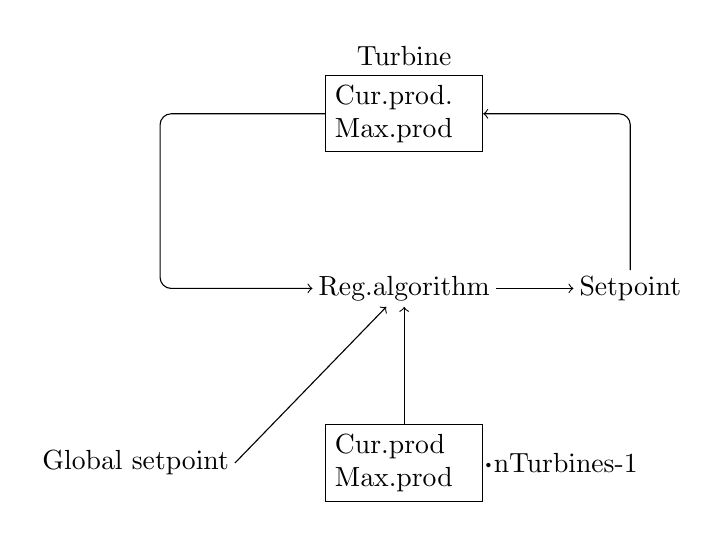
\begin{tikzpicture}[
	point/.style={inner sep=0pt}, %circle,minimum size=2pt,fill=red},
	textNode/.style={inner sep=2pt},
	hv path/.style={to path={-| (\tikztotarget)}},
	vh path/.style={to path={|- (\tikztotarget)}},
	skip loop h/.style={to path={-- ++(0,#1) -| (\tikztotarget)}},
	skip loop v/.style={to path={-- ++(#1,0) |- (\tikztotarget)}},
	graphs/every graph/.style={edges=rounded corners}
	]
	
% Place nodes
\matrix[row sep=1.5cm,column sep=.5cm] {
	\node [point]  		(p1x1)	{}; &&
	\node [rectangle]	(Turbine)		[draw, label=above:Turbine, text width=50pt]	{Cur.prod. Max.prod}; &&
	\node [point]  		(p1x3)	{}; \\
	
	\node [point]  		(p2x1)			{}; &&
	\node [textNode]	(HPPP)		 	{Reg.algorithm}; &&
	\node [textNode]	(Setpoint)	{Setpoint}; \\

	\node [textNode]  (gSetpoint)										{Global setpoint}; &&
	\node [rectangle]	(Data)			[draw, text width=50pt] {Cur.prod  Max.prod};\\
};

\node [textNode,right of=Data] {~~~~~~~~~~~~~~~~~\textbf{$\cdot$}nTurbines-1};
	
\graph[use existing nodes]{
	Turbine ->[skip loop v=-3.1cm] HPPP -> Setpoint ->[vh path] Turbine;
	gSetpoint.east -> HPPP;
	Data -> HPPP;
};

\end{tikzpicture}

	\captionsetup{format=plain,font=footnotesize,labelfont={bf,defaultCapFont},labelsep=quad,singlelinecheck=no}
	\caption[Decentralized input/output parameters of the regulation algorithm]{
		\label{fig:ioDecenRegAlg} 
		\footnotesize{%
			Decentralized input/output parameters of the regulation algorithm.
		}
	}
\end{figure}

The regulation algorithm is now computed on every turbine instead of computing the algorithm on a central Park Pilot. Thus, instead of requesting all states (current production and max production) externally, the regulation algorithm now collects one state from the local turbine. Furthermore the regulation algorithm only calculates a single setpoint - the setpoint used by the local turbine to set a new state - instead of calculating a setpoint for every turbine in the wind farm.

As \cref{fig:ioDecenRegAlg} implies, with the regulation algorithm performed on every turbine, decentralizing the Park Pilot onto the turbines also means that every turbine must know the state of every other turbine in the wind farm.

\section{Regulation cycle}

Decentralizing the Park Pilot onto the turbines has changed the regulation cycle too. The decentralized solution has been built with focus on scalability, in terms of increasing the number of turbines does not impact the regulation cycle, as well as performance, in terms of decreasing the regulation cycle time.

The following sections presents the decentralized regulation cycle. First by describing how the decentralized regulation cycle differs from the centralized regulation cycle, followed by a detailed description of how a single regulation cycle has been implemented. 

%Finally the term \textit{cache reads} is discussed, which is introduced by the decentralized by a discussion of the introduction of cache reads.

\subsection{Changes compared to the centralized regulation cycle}\label{sec:regCycleChanges}

The difference between the centralized regulation cycle and the decentralized regulation cycle is illustrated in \cref{fig:cycleCentralVSDecentral}. 

\begin{figure}[!h]
	%The figure show how regulation time differs central vs decantral

	{\sffamily{Centralized regulation cycle}}
	\newline
	

{ %The brackets issolate the enviroment

\tikzstyle{line}		 	= [draw]

\makeatletter
\ifcsname c@wavenum\endcsname %Only create one counter
\else
	\newcounter{wavenum}
\fi
\makeatother

\newcommand*{\bitvector}[3]{
  \draw[fill=#3] (t_cur) -- ++( .1, .3) -- ++(#2-.2,0) -- ++(.1, -.3)
                         -- ++(-.1,-.3) -- ++(.2-#2,0) -- cycle;
  \path (t_cur) -- node[anchor=mid](textNode) {#1} ++(#2,0) node[time] (t_cur) {};
  }

% \known{val}{length}
\newcommand*{\known}[2]{
    \bitvector{#1}{#2}{white}
}

% \unknown{length}
\newcommand*{\unknown}[2]{
    \bitvector{#1}{#2}{black!20}
}

% \nextwave{name}
\newcommand{\nextwave}[1]{
  %\path (0,\value{wavenum}) node[time] (t_cur) {};
   \path (0,\value{wavenum}) node[left] {#1} node[time] (t_cur) {};
  \addtocounter{wavenum}{-1}
}

\newcommand{\timeSpanLabel}{
	\node (CycleTimeLabel) [rectangle, above = 0.7cm of textNode, inner sep=0pt] {Regulation cycle time};	  
}

\newcommand{\timeSpanA}{
	\node (t_timeSpanA) [point, above = 0 of t_cur] {};	  
}

\newcommand{\timeSpanB}{
	\node (t_timeSpanB) [point, above =0 of t_cur] {};

  \graph[use existing nodes]{
  	t_timeSpanA --[time span=1cm] CycleTimeLabel;
   	CycleTimeLabel.south --[time span=-0.24cm] t_timeSpanB;
  }; 
    	
}


%%% End of timing.sty
\begin{tikzpicture}[
	point/.style={inner sep=0pt}, %circle,minimum size=2pt,fill=red},
	draw=black, 
	yscale=.8,
	xscale=1,
	hv path/.style={to path={-| (\tikztotarget)}},
	vh path/.style={to path={|- (\tikztotarget)}},
	skip loop v/.style={to path={-- ++(#1,0) |- (\tikztotarget)}},		
	skip loop h/.style={to path={-- ++(0,#1) -| (\tikztotarget)}},
	time span/.style={to path={-- ++(0,#1) -| (\tikztotarget)}},
	graphs/every graph/.style={edges=rounded corners}	
	]
	
  \tikzstyle{time}=[coordinate]
  \setlength{\unitlength}{1cm}
  \setcounter{wavenum}{0}
    
  %\nextwave{Regulation Time} \unknown{SendData}{2} \known{WaitForData}{5} \unknown{ReciveData}{2} \unknown{Calculate}{2}\unknown{SendSP}{2}
  \nextwave{Park Pilot} \unknown{reqStates}{1.8} \known{wait}{2} \unknown{readStates}{2} \unknown{regAlg.}{1.7} \unknown{sendSetpoints}{2.6}
  
  \nextwave{Turbine} \known{wait}{1.8} \unknown{replyState}{2} \known{wait}{6.3} \unknown{receiveSetpoint}{2.9}
    
  
\end{tikzpicture}
}

	\newline
	
	{\sffamily{Decentralized regulation cycle (with parallel reception of data)}}
	\newline
	

{ %The brackets issolate the enviroment

\makeatletter
\ifcsname c@wavenum\endcsname %Only create one counter
\else
	\newcounter{wavenum}
\fi
\makeatother

\newcommand*{\bitvector}[3]{
  \draw[fill=#3] (t_cur) -- ++( .1, .3) -- ++(#2-.2,0) -- ++(.1, -.3)
                         -- ++(-.1,-.3) -- ++(.2-#2,0) -- cycle;
  \path (t_cur) -- node[anchor=mid](textNode) {#1} ++(#2,0) node[time] (t_cur) {};
}

% \known{val}{length}
\newcommand*{\known}[2]{
    \bitvector{#1}{#2}{white}
}

% \unknown{length}
\newcommand*{\unknown}[2]{
    \bitvector{#1}{#2}{black!20}
}

% \nextwave{name}
\newcommand{\nextwave}[1]{
  %\path (0,\value{wavenum}) node[left] {#1} node[time] (t_cur) {};
  %\path (0,\value{wavenum}) node[time] (t_cur) {};
  \path (0,\value{wavenum}) node[below left] {#1} node[time] (t_cur) {};
  \addtocounter{wavenum}{-1}
}


\newcommand{\timeSpanA}{
	\node (t_timeSpanA) [point, above = 0 of t_cur] {};	  
}

\newcommand{\timeSpanB}{
	\node (t_timeSpanB) [point, above =0 of t_cur] {};
	
	\graph[use existing nodes]{
		t_timeSpanA --[time span=1cm] CycleTimeLabel;
		CycleTimeLabel.south --[time span=-0.24cm] t_timeSpanB;
	}; 
	
}

%%% End of timing.sty

\begin{tikzpicture}[
	point/.style={inner sep=0pt}, %circle,minimum size=2pt,fill=red},
	draw=black, 
	yscale=.8,
	xscale=1,
	hv path/.style={to path={-| (\tikztotarget)}},
	vh path/.style={to path={|- (\tikztotarget)}},
	skip loop v/.style={to path={-- ++(#1,0) |- (\tikztotarget)}},		
	skip loop h/.style={to path={-- ++(0,#1) -| (\tikztotarget)}},
	time span/.style={to path={-- ++(0,#1) -| (\tikztotarget)}},
	graphs/every graph/.style={edges=rounded corners}	
]
	
\tikzstyle{time}=[coordinate]
\setlength{\unitlength}{1cm}
\setcounter{wavenum}{0}

	\nextwave{Turbine} \unknown{readStates}{2.5} \unknown{regAlg.}{2.5} \unknown{setSetpoint}{2.5} \unknown{sendState}{2.5} \known{sleep}{2}
	\nextwave{} \known{reciveStates}{12}
\end{tikzpicture}
}

	\caption{Centralized vs decentralized regulation cycle}
	\label{fig:cycleCentralVSDecentral}
\end{figure}

In the centralized solution a request for data and waiting for the corresponding reply for every turbine was a requirement for the Park Pilot, turbines in the decentralized solution publish new states whenever a new setpoint has been calculated. Turbines publishes to a specific Topic and are assigned a unique keys. Receiving states from other turbines is handled and loaded asynchronously into memory by Connext, thus receiving states is a parallel process running alongside the regulation algorithm.
This enables a \textit{Distributed Shared Memory (DSM)} (see \cref{sec:DSM} for DSM description) behavior for the decentralized solution, where the state of every turbine is shared with every other turbine in the wind farm.
As every turbine has a unique Topic key, each turbine has assigned its own shared memory space, where only the turbine is allowed to write, as illustrated in \cref{fig:DSMlikeBehavior}, thus removing the possibility that turbines overwrite each others states. Using DSM like behavior for the decentralized solution, means that receiving states from other turbines is abstracted away from the regulation cycle, enabling the turbines to assume that the latest state of every other turbine has been received and is available locally in memory. This alleviates the need for the request-reply part of the centralized regulation cycle. The expectation is that removing the request-reply part of the algorithm decreases the regulation cycle time, since acquisition of turbine states are no longer a part of the regulation cycle.  

\begin{figure}[!h]
	\begin{tabular}{ | c | c | c | c | c |}
		\cline{1-3}
		\cline{5-5}
		turbine 1 & turbine 2 & turbine 3 & \dots & turbine n \\
		\cline{1-3}
		\cline{5-5}
	\end{tabular}
	\caption{Distributed Shared Memory like behavior of the decentralized solution}
	\label{fig:DSMlikeBehavior}
\end{figure}

Removing the request-reply part of the regulation cycle for the decentralized solution, also removes the ability to ensure that regulation happens using latest states only, since a given turbine, when initiating the regulation cycle, reads the turbine states that is already in memory, instead of requesting all the latest states. This of course forces a redefinition of when a state is usable for regulation. Instead of using latest states only, the decentralized solution defines a time limit that, when reached, changes the status of the state to old and thus not usable for regulation. Thus for the decentralized solution it is acceptable to perform regulation using states that are no older than the specified time limits. 

To further decrease the regulation cycle time, strictly reliable messaging has been removed from the decentralized solution. A reply from all turbines at a specific point in the regulation cycle is no longer needed, thus package loss will no longer block the regulation cycle. Furthermore, with the time limit introduced, all states are no longer needed by every turbine, since states now only have to be strictly 'younger' than the specified time limit.
Instead of strictly reliable messaging the decentralized solution use best effort messaging, where data samples are sent once and missed samples are acceptable. As every turbine of the decentralized solution only relies on the newest published state and not every state published, a dropped state is no longer critical as it is overwritten by the state of the next regulation cycle for a given turbine.

Finally multicast has been enabled for the decentralized solution to greatly reduce the number of packages each turbine sends, when publishing a new state. With multicast enabled only one package is sent pr. new state, as opposed to the centralized solution which sends a package per receiver. This reduces the load of each turbine and decreases the regulation cycle time. Furthermore, this also reduces overall network traffic.  

Each turbine only calculate it's own setpoint. Thus after calculation, the new setpoint is set locally and the new state is published to the other turbines. The wait time at the end of the regulation cycle is needed in order to leave a small amount of time for Connext to receive and overwrite states that have already been read.

\subsection{Implementation}

Before running the regulation cycle illustrated in \cref{fig:decenRegCycle}, an initial setpoint is set and the corresponding state of the turbine is read, enabling publishing of the turbine state as the first step of the regulation cycle. This is done to prevent the first cycle from being redundant due to lack of data from other turbines. 

\begin{figure}[!h]
	\centering
	\begin{sequencediagram} %Created using pgf-umlsd
		\newthread{parkPilot}{:Park Pilot}
		\newinst[2]{turbine}{:Turbine}
		\newinst[2]{connext}{:Connext}
		
		\begin {messcall}{parkPilot}{publishState()}{connext}{}
		\end {messcall}
		\begin {call}{parkPilot}{readStates()}{connext}{states}
		\end {call}
		\begin {callself}{parkPilot}{regAlgorithm()}{setpoint}
		\end {callself}
		\begin {call}{parkPilot}{sendSetpoint()}{turbine}{setpoint}
		\end {call}
		\begin {call}{parkPilot}{readState()}{turbine}{state}
		\end {call}	
		\begin {callself}{parkPilot}{sleep()}{}
		\end {callself}			
	\end{sequencediagram}

	\captionsetup{format=plain,font=footnotesize,labelfont={bf,defaultCapFont},labelsep=quad,singlelinecheck=no}
	\caption[Decentralized regulation cycle sequence diagram]{
		\label{fig:decenRegCycle} 
		\footnotesize{%
			Decentralized regulation cycle sequence diagram.
		}
	}
\end{figure}

\Cref{fig:decenRegCycle} presents three objects:

\begin{itemize}
	\item The \textbf{Park Pilot} object which handles the regulation cycle. As opposed to the centralized solution, the Park Pilot object is now instantiated on every turbine in the wind farm, instead of being a single external component.
	\item The \textbf{Turbine} object which serves as the interface to the underlying Turbine. The Turbine object for the purpose of this thesis is just a simulation of an actual turbine. Thus this object handles communication with a database with actual turbine data provided by Siemens Wind Power.
	\item \textbf{Connext} is the underlying DDS framework used for communication, thus this is not an object instantiated by the Park Pilot. It is however what enables reception of data in parallel with the regulation cycle. 
\end{itemize}

The Park Pilot publishes the state of the present turbine and reads the states of every turbine within the wind farm. Afterwards the regulation algorithm is performed and a setpoint for the present turbine is calculated and used to set a new state.

The regulation algorithm used for the decentralized solution is the same used for the centralized solution described in \cref{sec:calculateSetpoints}, with the exception that the setpoint calculated is kept for local purposes instead of sending the setpoint to all turbines. The regulation algorithm code for the decentralized solution is presented in \cref{fig:decenRegAlgCode}.

\begin{figure}[!h]
	\centering
%	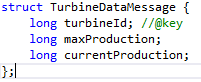
\includegraphics[width=0.3\textwidth,natwidth=250,natheight=200]{turbineDataMessage.PNG} 
	\begin{lstlisting}[language=C++,tabsize=2,basicstyle=\small]
uint_fast32_t DecentralizedParkPilot::regAlgorithm(
	uint_fast32_t globalSetpoint,
	TurbineMessageSeq turbines,
	uint_fast32_t maxProd,
	uint_fast32_t currentProd,
	uint_fast32_t setPoint,
	DDS_SampleInfoSeq turbineInfos,
	uint_fast32_t &cacheCount )
{
	cacheCount = 0;
	if (currentProd >= maxProd)
		return maxProd;

	int availableTurbinesCount = turbines.length();

	for (int i = 0; i < turbines.length(); i++)
	{
		if (!turbineInfos[i].valid_data) {
			availableTurbinesCount--;
			continue;
		}

		if (turbineInfos[i].sample_state == DDS_READ_SAMPLE_STATE) {
			cacheCount++;
		}

		if (turbines[i].currentProduction >= turbines[i].maxProduction)
			availableTurbinesCount--;
	}
	uint_fast32_t localSetpoint = 0;

	if (availableTurbinesCount <= 0)
		localSetpoint = globalSetpoint;
	else
		localSetpoint = globalSetpoint / availableTurbinesCount;

	if (localSetpoint > maxProd) {
		localSetpoint = maxProd;
	}

	return localSetpoint;
}
	\end{lstlisting}
	\captionsetup{format=plain,font=footnotesize,labelfont={bf,defaultCapFont},labelsep=quad,singlelinecheck=no}
	\caption[The regulation algorithm of the decentralized solution]{
		\label{fig:decenRegAlgCode} 
		\footnotesize{%
			Code for the decentralized regulation algorithm used to calculate setpoints.
		}
	}
\end{figure}

\subsection{Cache reads}\label{sec:cachereads}

A cache read happens if the cycle time elapses before all turbine instances have responded with state information, resulting in the same state being read twice. Thus it is a natural result of separating receiving data from the regulation cycle, as done in the decentralized solution. Connext only keeps track of data that has already been read but not how many times that data has been read. Thus a cache read does not include information regarding if the same state has been read multiple times.

The regulation cycle of the decentralized solution does not directly include any communication, thus enabling a significant reduction of regulation cycle time. However, decreasing the cycle time, increases the 'pressure' on Connext by increasing the number of regulation cycles pr. minute, thus increasing the number of states that needs to be published, thus increasing the number of states that needs to be received (assuming that the cycle time of all turbines are equally decreased). This ultimately results in increased number of cache reads and increased network traffic. Thus decreasing the regulation cycle time will increase the number of cache reads.  

Increasing the number of cache reads can be an issue, since it reduces the effectiveness of the regulation cycle. Having a high number of cache reads implies that the regulation has been performed using data used for the previous regulation, thus decreasing the effect of the current regulation.

As a result of this trade-off between reduction in regulation cycle time and number of cache reads, a sleep is introduced at the end of the regulation cycle (as presented in \cref{fig:decenRegCycle}), in order to control the reduction of the regulation cycle. Thus the regulation cycle time is an input parameter of the decentralized solution.

\section{DDS configuration} \label{sec:decen:ddsconf}

The key component used for communication is DDS (see \cref{sec:DSM} for DDS description). This section describes how DDS has been configured for the decentralized solution.

\subsection{Interface Definition Language}\label{sec:decenIdl}

As with the centralized solution, Interface Definition Language (IDL) has been used for generating Data Transfer Objects for the decentralized solution. See centralized IDL \cref{sec:cenIdl} for details.

\begin{figure}[!h]
	\centering
	%	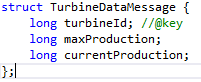
\includegraphics[width=0.3\textwidth,natwidth=250,natheight=200]{turbineDataMessage.PNG} 
	\begin{lstlisting}[language=C++,tabsize=2,basicstyle=\small]
	struct TurbineMessage {
		long turbineId; //@key
		long maxProduction;
		long currentProduction;
		long setPoint;
		long msSinceLastWrite;
		long cacheCount;
	};	
	\end{lstlisting}
	\captionsetup{format=plain,font=footnotesize,labelfont={bf,defaultCapFont},labelsep=quad,singlelinecheck=no}
	\caption[Decentralized turbine message]{
		\label{fig:decenTurbineMessage} 
		\footnotesize{%
			The turbine message .idl file sent from the turbines to all other turbines in the decentralized solution.
		}
	}
\end{figure}

\subsection{Choosing Quality of Service parameters}\label{sec:decenChoosingQoS}

The Quality of Service (QoS) parameters for the decentralized solution is based on the QoS parameters determined for the centralized solution, except for the following key areas:

\begin{description}
	\item[Reliability] of messaging has been changed to best effort messaging in order to reduce the regulation cycle time. This means package drops are allowed for the decentralized solution.
	\item[Durability] of the decentralized solution has been changed to local durability. This means that the current state of every turbine is sent to newly discovered turbines. Note that with best effort messaging there is no guarantee that the states are received, since package drops are allowed. Durability for the regulation cycle has only minor relevance, since newly arrived turbines will receive all states within a short amount of time after being discovered. Thus this setting has only been applied, since an attempt to receive states upon startup is better than receiving no states at all. However, for real life purposes, the turbines should probably be configured with a default setpoint, which is used until data from all turbines has been received, in combination with this setting. 
	\item[Throughput] remains the same as the throughput setting of the centralized solution but for a slightly different reason. New turbine states must be sent as soon as possible, which removes the need for batching. \todo{Hvorfor gør det batching irrelevant?} Thus regular throughput has been chosen for the decentralized solution. 
	\item[Multicast] has been enabled to reduce regulation cycle time and network traffic, as explained in \cref{sec:regCycleChanges}.
\end{description}

\subsection{Detailed quality of service evaluation}

This section provides a detailed evaluation of every parameter used for the decentralized QoS XML. The full QoS XML is presented but only parameter changes from the centralized solution are discussed.

\paragraph{Participant factory} (\cref{fig:decParFacQos}) QoS parameters has been set to be the same as the centralized solution. See Participant factory description of \cref{sec:detailedQoSDesc}.

\begin{figure}[!h]
\begin{lstlisting}[language=XML]
<participant_factory_qos>
	<logging>
		<verbosity>WARNING</verbosity>
		<category>PLATFORM</category>
		<print_format>VERBOSE_TIMESTAMPED</print_format>
		<output_file>ddsadaptor.log</output_file>
	</logging>
</participant_factory_qos>
\end{lstlisting}
\caption[Decentralized participant factory QoS parameters]{
		\label{fig:decParFacQos} 
		\footnotesize{Participant factory QoS parameters of the decentralized solution.}
	}
\end{figure}

\paragraph{Participant} (\cref{fig:decParQos}) QoS parameters has been evaluated as follows (see Participant evaluation of \cref{sec:detailedQoSDesc} for parameters not described):

\begin{itemize}
	\item \textbf{.builtin.multicast\_enabled} value has been set to 1 to enable multicast.
\end{itemize}

\begin{figure}[!h]
\begin{lstlisting}[language=XML]
<participant_qos>
	<participant_name>
		<name>TurbineParticipant</name>
		<role_name>TurbineParticipantRole</role_name>
	</participant_name>
		<database>
		<shutdown_cleanup_period>
			<sec>DURATION_ZERO_SEC</sec>
			<nanosec>1</nanosec>
		</shutdown_cleanup_period>
	</database>
		<transport_builtin>
			<mask>UDPv4</mask>
		</transport_builtin>
	<property>
		<value>
			<element>
				<name>dds.transport.UDPv4.builtin.multicast_enabled</name>
				<value>1</value>
			</element>
			<element>
				<name>dds.transport.UDPv4.builtin.parent.message_size_max</name>
				<value>65535</value>
			</element>
			<element>
				<name>dds.transport.UDPv4.builtin.send_socket_buffer_size </name>
				<value>65535</value>
			</element>
			<element>
				<name>dds.transport.UDPv4.builtin.recv_socket_buffer_size</name>
				<value>2097152</value>
			</element>
		</value>
	</property>
</participant_qos>
\end{lstlisting}
\caption[Decentralized participant QoS parameters]{
		\label{fig:decParQos} 
		\footnotesize{Participant QoS parameters of the decentralized solution.}
	}
\end{figure}

\paragraph{Topic} (\cref{fig:decTopicQos}) QoS parameters are used to initialize DataReader and DataWriter QoS paramters. Thus parameters that applies to both DataReaders and DataWriters have been configured using a Topic profile. Topic QoS parameters have been evaluated as follows:

\begin{itemize}
	\item \textbf{reliability} of the decentralized solution has been set to best effort, as discussed in \cref{sec:decenChoosingQoS}, thus making package drops acceptable.
	\item \textbf{durability} has been set to local durability, thus latest states from all online turbines are sent to newly added turbines.
	
	Note that in combination with best effort reliability, a newly added turbines is not ensured all turbine states. Furthermore the amount of states received from each turbines is the depth value set by the history QoS parameter.
	\item \textbf{history} configures the number of data samples the send and receive buffers can contain on a per instance basis for keyed Topics. With KEEP\_LAST\_HISTORY\_QOS enabled, the latest values of the data samples are kept and old samples are discarded when the limit as set by the depth parameter is reached. Thus the send and receive buffers of the decentralized solution acts like a circular buffer of length 1, meaning, in combination with best effort messaging, only newest states are available to the turbines.
\end{itemize}

\begin{figure}[!h]
\begin{lstlisting}[language=XML]
<topic_qos name="TurbineTopicQos">
	<reliability>
		<kind>DDS_BEST_EFFORT_RELIABILITY_QOS</kind>
	</reliability>
	<durability>
		<kind>TRANSIENT_LOCAL_DURABILITY_QOS</kind>
	</durability>
	<history>
		<kind>KEEP_LAST_HISTORY_QOS</kind>
		<depth>1</depth>
	</history>
</topic_qos>
\end{lstlisting}
\caption[Decentralized Topic QoS parameters]{
		\label{fig:decTopicQos} 
		\footnotesize{Topic QoS parameters of the decentralized solution.}
	}
\end{figure}

\paragraph{DataWriter} (\cref{fig:decDataWriterQos}) QoS parameters has been evaluated as follows (see DataWriter evaluation of \cref{sec:detailedQoSDesc} for parameters not described):

\begin{itemize}
	\item \textbf{lifespan} configures the expiration time of each data sample written by a DataWriter. Thus this parameter is only relevant to DataWriters. Each data sample has an associated expiration time, beyond which the data should not be delivered. Once the sample expires, the data sample will be removed from the DataReaders receive buffers. 
	
	This parameter configures the previously mentioned time limit (\cref{sec:regCycleChanges}) of the decentralized solution. A turbine state expires after 150000000 nanoseconds ($=150$ ms). This value is set after the worst case regulation cycle time of the current Siemens system, to ensure that the decentralized solution do not use data older than what the current Siemens system use for regulation.
	
	Furthermore, this parameter also indirectly controls how many and which turbines should be used for the regulation algorithm. If a state is older than 150 ms, the state is automatically removed from the receive buffer, thus it is removed from the data that is read and used for the regulation algorithm. As the regulation algorithm automatically scales with the number of turbines, from which a state has been received within the latest 150 ms, the turbine which have not sent a new state within 150 ms will be considered offline. For this reason the lifespan parameter is responsible for the tolerance of the decentralized solution. If a turbines fails, the state of the turbine will eventually expire, thus removing the turbine from the regulation algorithm.
\end{itemize}

\begin{figure}[!h]
\begin{lstlisting}[language=XML]
<datawriter_qos>
	<publication_name>
		<name>TurbineDataWriter</name>
	</publication_name>
	<lifespan>
		<duration>
			<sec>0</sec>
			<nanosec>150000000</nanosec>
		</duration>
	</lifespan>
</datawriter_qos>
\end{lstlisting}
\caption[Decentralized DataWriter QoS parameters]{
		\label{fig:decDataWriterQos} 
		\footnotesize{DataWriter QoS parameters of the decentralized solution.}
	}
\end{figure}

\paragraph{DataReader} (\cref{fig:decDataReaderQos}) QoS parameters has been evaluated as follows (see DataReader evaluation of \cref{sec:detailedQoSDesc} for parameters not described):

\begin{itemize}
	\item \textbf{multicast} specifies the multicast addresses on which DataReaders receives data from DataWriters. 
\end{itemize}

\begin{figure}[!h]
\begin{lstlisting}[language=XML]
<datareader_qos>
	<subscription_name>
		<name>TurbineDataReader</name>
	</subscription_name>
	<multicast>
		<kind>AUTOMATIC_TRANSPORT_MULTICAST_QOS</kind>
		<value>
			<element>
				<receive_address>239.192.0.1</receive_address>
			</element>
		</value>
	</multicast>
</datareader_qos>
\end{lstlisting}
\caption[Decentralized DataReader QoS parameters]{
		\label{fig:decDataReaderQos} 
		\footnotesize{DataReader QoS parameters of the decentralized solution.}
	}
\end{figure}
\chapter{Graphical user interface} \label{sec:graphicalInterface}
This chapter describes a graphical user interface created to visualize the power production of the turbines in the decentralized solution. Furthermore, DDS Blockset for Simulink is presented and how it is used to capture and log data from both the centralized and the decentralized solution.

The graphical user interface has been constructed using Matlab, Simulink and DDS Blockset for Simulink.
These tools combined allows the creation of a Simulink model which taps into the communication of the DDS framework.
The data collected via the Simulink models can then be transferred to Matlab for further processing or visualization.

The main objective of the graphical interface is to visualize what messages is currently flowing in the system but almost as important is the ability to collect data for further analysis.
Matlab is a powerful tool for anlysis and having data transferred live from the DDS framework to Matlab allows for both live as well as in depth analysis on datasets collected during experiments.

Currently only the decentralized solution can be visualized and controlled using the graphical interface. Given the scope and focus of this thesis the value added by visualizing the centralised solution would be minimal. Both the decentralized and centralized solutions are able to log data using the Simulink models.

\section{DDS Blockset for Simulink}
RTI has created a Blockset for Simulink allowing a Simulink model to interact with the DDS Participant and other entities in a DDS enabled network.
The blockset consists of a toolbox containing 6 blocks. Common for all blocks except the DDS Time block is that they can be configured with a default or custom Quality of Service (QoS) profile as well as a sample time. The QoS profile must match the QoS profile used in the network which the Simulink model is to interact with. The sample time is related to the Simulink model and specifies the timeinterval between samples.

\begin{figure}[h]
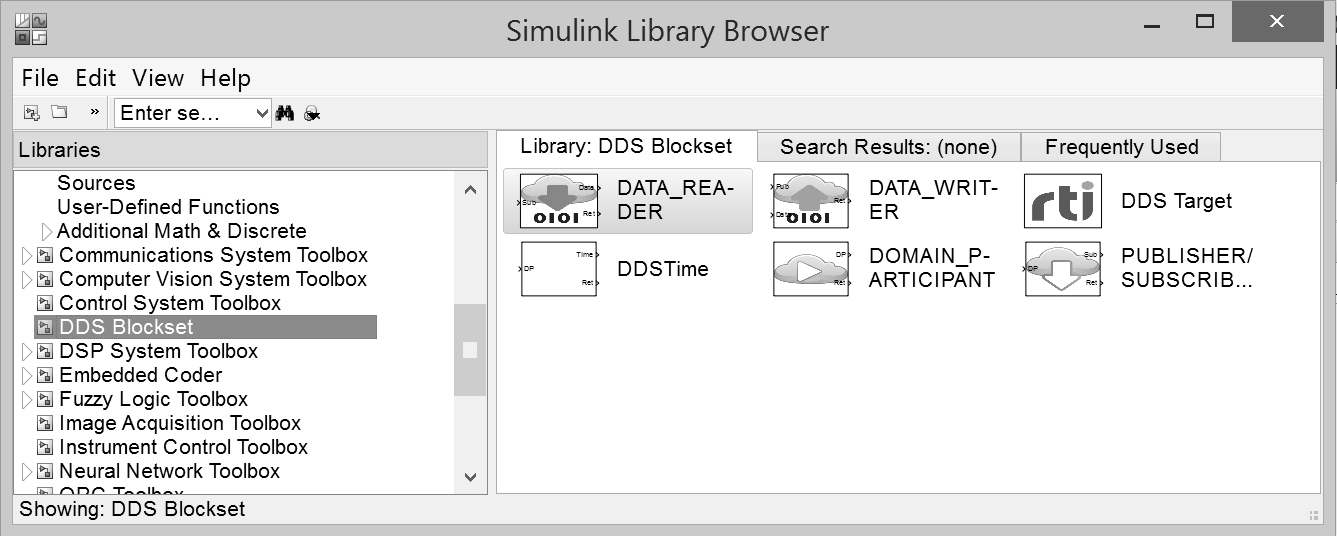
\includegraphics[width=\textwidth]{figures/DDSBlockset}
\captionsetup{format=plain,font=footnotesize,labelfont={bf,defaultCapFont},labelsep=quad,singlelinecheck=no}
	\caption[DDSBlockset blocks for Simulink]{
		\label{fig:DDSBlocksetBlocks} 
		\footnotesize{%
			DDSBlockset blocks for Simulink.
		}
	}
\end{figure}


\paragraph{The DomainParticipant block} is the equivalent to the \textit{DomainParticipant} entity in DDS. This block allows for configuration of a DomainID which links the \textit{DomainParticipant} to a specific DDS domain.

\paragraph{The Publisher/Subscriber block} can be configured as either a \textit{Publisher} or a \textit{Subscriber} and will act as either based on the chosen configuration.

\paragraph{The DataWriter block} is the equivalent to the \textit{DataWriter} entity in DDS. This block can write data to a \textit{Topic} in DDS. The DataWriter block must be configured with the name of the \textit{Topic} as well as the name of the Topic Type created by the Simulink Bus that is input to the DataWriter.

\paragraph{The DataReader block} is the equivalent to the \textit{DataReader} entity in DDS. This block can read data from a \textit{Topic} in DDS. The DataReader block must be configured with the name of the \textit{Topic} as well as the name of the Topic Type created by the Simulink Bus that is input to the DataReader block. The DataReader block can also be configured to either use Read() or Take() for obtaining data from DDS. The Read() command will leave copy data from DDS memory, the Take() command will remove the data from DDS memory. The DataReader block is able to either poll DDS for data, or wait until data is ready or a timeout occurs.

\paragraph{The DDSTarget block} controls how code is generated for the DDS blocks in the Simulink model. It is possible to configure which version of DDS code will be generated for, either RTI Connext DDS(default), or RTI Connext Micro DDS. The type system can be configured to either static or dynamic as well as the discovery mode.

\paragraph{The Time block} returns the current time from DDS output in seconds and nanoseconds.

\section{Simulink model of the decentralized solution}\label{subsec:decentralizedmodel}

\begin{figure}[!h]
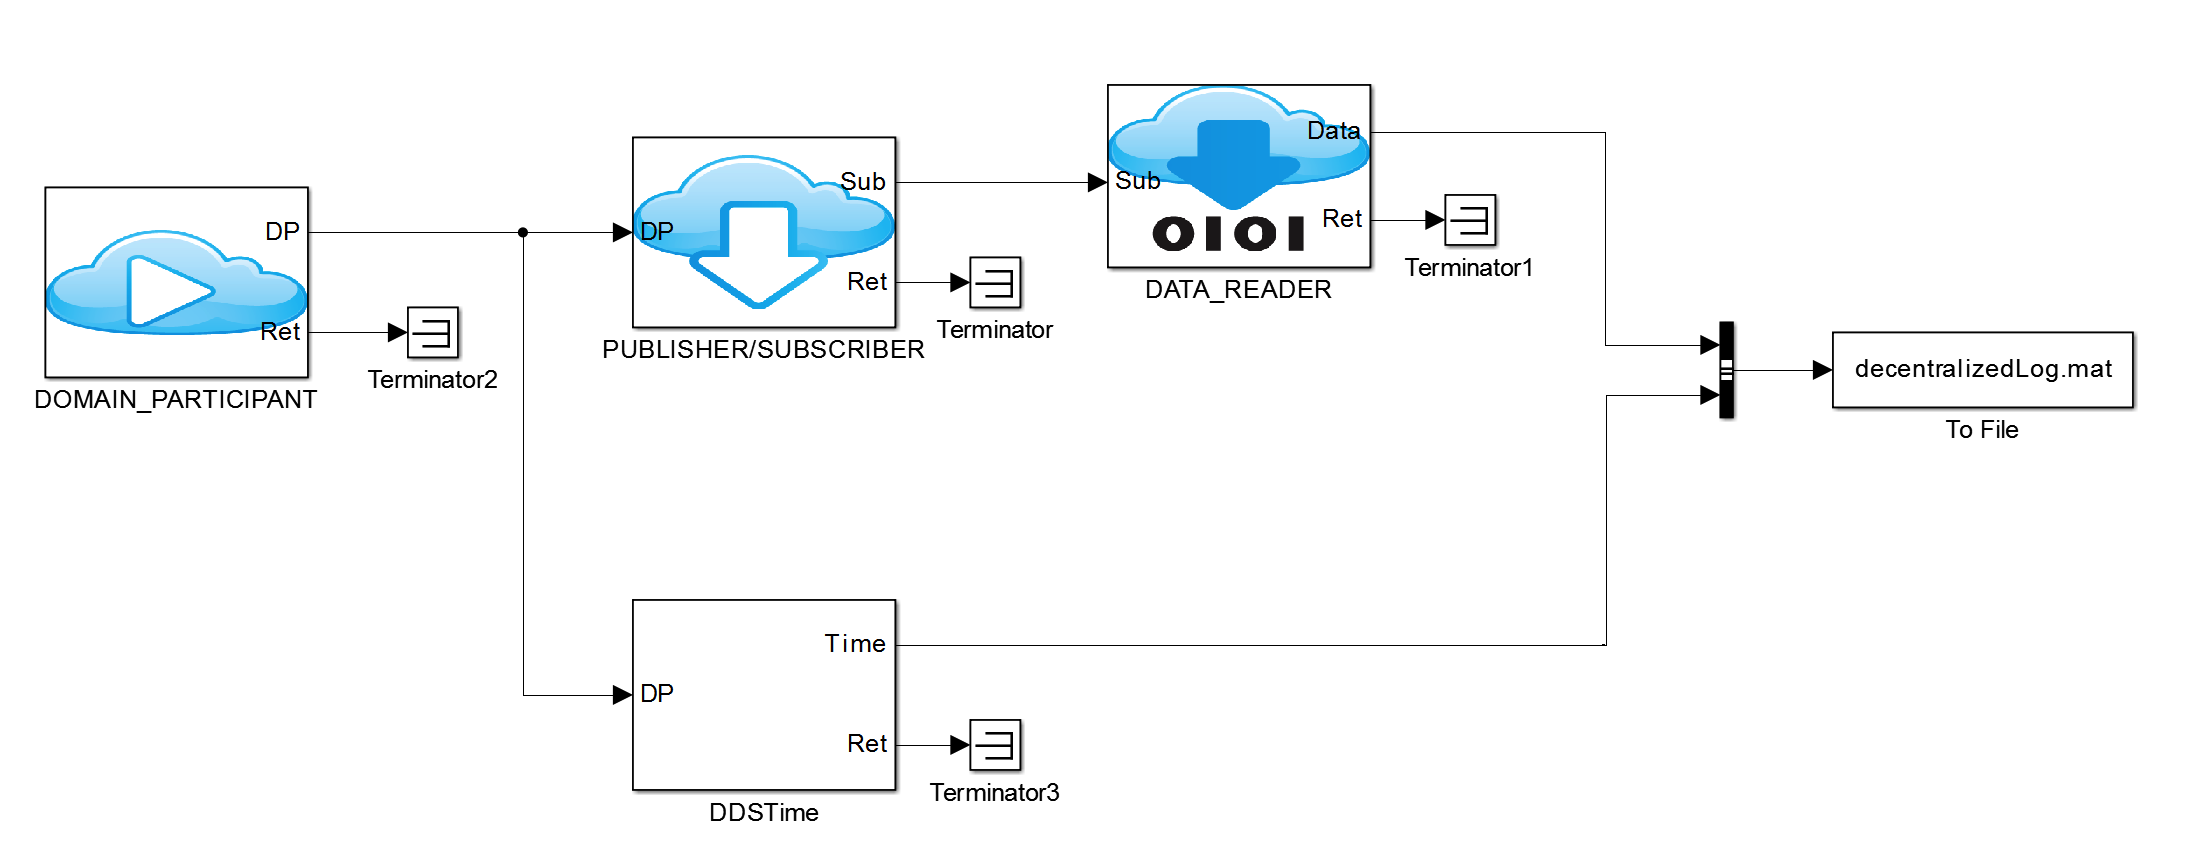
\includegraphics[width=\textwidth]{figures/DecentralizedModel}
\captionsetup{format=plain,font=footnotesize,labelfont={bf,defaultCapFont},labelsep=quad,singlelinecheck=no}
	\caption[Decentralized Simulink model]{
		\label{fig:decentralizedSimulinkModel} 
		\footnotesize{%
			Decentralized Simulink model.
		}
	}
\end{figure}

The Simulink model of the decentralized solution is simple. The decentralized Simulink model has a DomainParticipant block in order to be able to receive data from the same domain as the turbines. It also has a Time block to enable logging and graphing of the current DDS time. Since the decentralized solution only uses one DDS message type, TurbineMessage \cref{sec:decenIdl}, to communicate between the turbines in the system, the decentralized Simulink model has only one Subscriber block and one DataReader block. The Subscriber block specifies the Topic to subscribe to and the DataReader block receives events every time a new TurbineMessage is available. The TurbineMessage that is received is logged to a .mat file together with the current DDS time for later use.

In order to transfer data from the Simulink model to Matlab eventlisteners must be implemented in a Matlab .m file. In the decentralized solution the eventhandler listens for incoming events on the bus object that receives new data from the DataReader block. When new data is received the event fires and data can be collected from the Simulink model. Furthermore, model execution can be controlled from Matlab, as well as parameters like model runtime.

\section{Simulink model of the centralized solution}\label{subsec:centralizedmodel}
The Simulink model of the centralized solution is a bit more complex. The centralized solution contains three different messagetypes, TurbineDataMessage, RequestMessage, SetpointMessage, \cref{sec:cenIdl} that all run on different topics. Because of this the centralized Simulink model contains one DomainParticipant, three Subscribers, one for each topic, and three DataReaders, one for each message type, in order to capture the communication in the centralized solution. Every message received is logged to a .mat file together with the current DDS time.

\begin{figure}[!h]
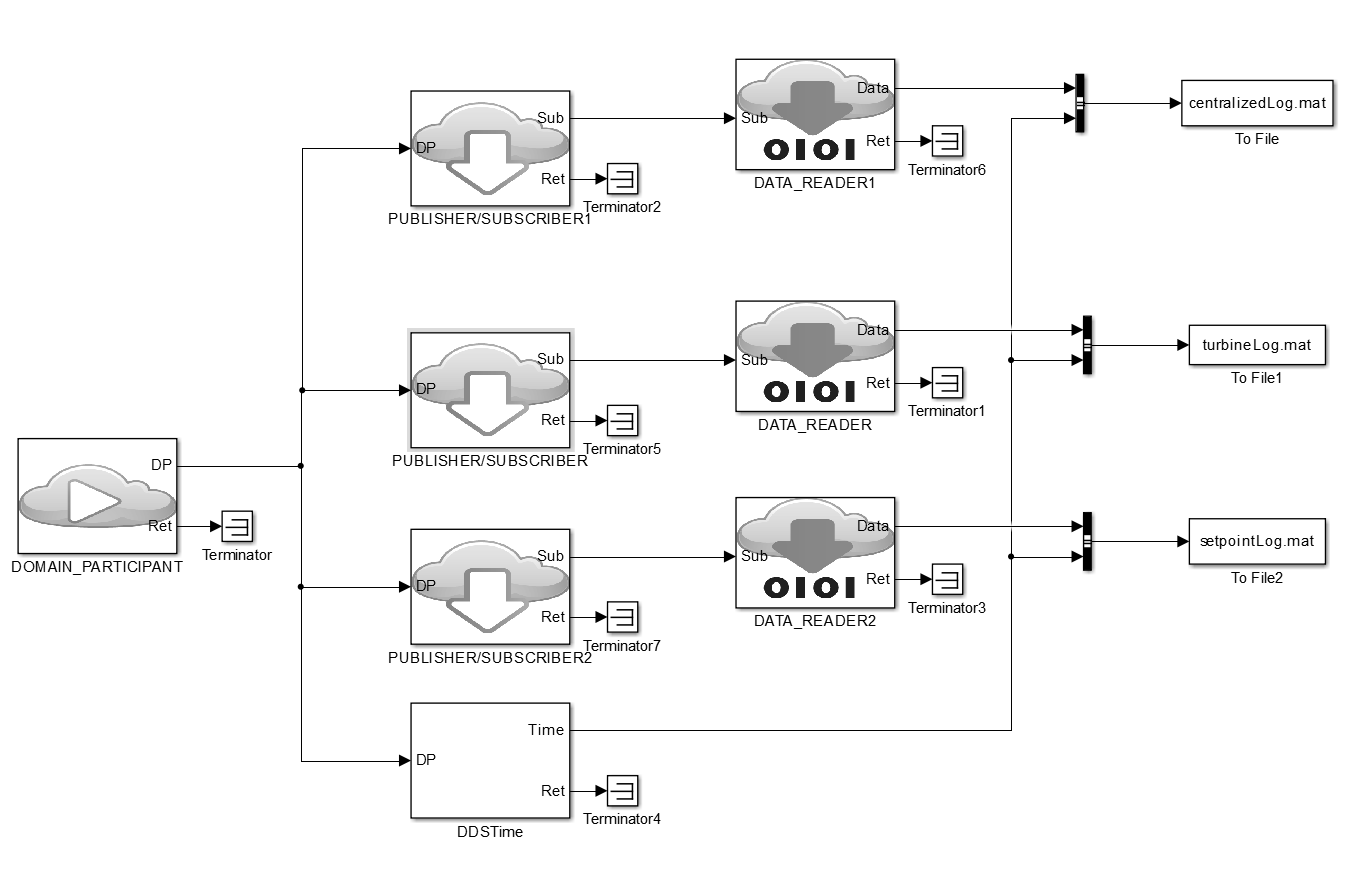
\includegraphics[width=\textwidth]{figures/CentralizedModel}
\captionsetup{format=plain,font=footnotesize,labelfont={bf,defaultCapFont},labelsep=quad,singlelinecheck=no}
	\caption[Centralized Simulink model]{
		\label{fig:centralizedSimulinkModel} 
		\footnotesize{%
			Centralized Simulink model.
		}
	}
\end{figure}

\section{Installation of DDS Blockset for Simulink}
To install DDS Blockset for Simulink follow the steps provided by Mathworks \cite{DDSBlocksetPilotSupportPackageUserGuide}. The installation is short but as described below additional work has to be done in order to make DDS Blockset for Simulink work properly with Matlab and Interface Definition Language files.

The problems described in the section all relates to installation of DDS Blockset for Simulink using Matlab 2013b on a Windows 8.1 x64 environment.
Other environments may be more or less optimal but have not been tested during this thesis.

There are a few caveats to be avoided when installing DDS Blockset for Simulink on Windows.
After installation of DDSBlockset for Simulink completes make sure the NDDSHOME path variable is set to \path{C:\Program Files(x86)\RTI}.
Notice that this path is different from the default path recommended by RTI which is \path{C:\Program Files(x86)\RTI\ndds.5.0.0} (version numbers may change).

DDS Blockset for Simulink has an import feature for import of Interface Definition Language files. The import process creates a Simulink bus that the Simulink model can hook into and pull data from. In order to enable import of Interface Definition Language files additional setup must be performed.
Since Matlab does not provide a compiler for C++ on x64 systems one must be downloaded. Microsoft provides a compiler in the Microsoft Windows SDK 7.1. Matlab must be told to use the compiler by using the \path{mex -setup} command. Finally the location of the binaries and the libraries that are downloaded with the new compiler must be added to path.
% !TeX spellcheck = en_US

\chapter{Experiments, results and discussion}
\label{cha:experiments}
This chapter contains the experiments, results and discussion of this thesis. A section of this chapter is devoted to each problem presented in \cref{sec:problemStatement}. Each section contains a description of the experiments performed to prove or disprove the problem, the results obtained from the experiment and a discussion of the results in relation to the original problem.

%The main goal of this thesis is to evaluate a decentralized solution for the current Siemens system. The decentralized solution is evaluated in terms of \ref{PS:Q:Feasibility}, \ref{PS:Q:Availability}, \ref{PS:Q:Performance} and \ref{PS:Q:Scalability} defined in \cref{sec:problemStatement}. \ref{PS:Q:Scalability} is evaluated against a centralized solution designed to be as similar to the current Siemens system as possible.
%To evaluate the decentralized solution, the experiments in the following sections where created. 
%The experiments are grouped by in relation to the problem statements proposed in \cref{sec:problemStatement}.

%The experiments are performed using three laptops connected using a Gbit(IEEE 802.3ab) Ethernet router with IGMP support. for hardware specifications see \cref{appendix:HardwareSpecification}, the laptops are using 100Mb(IEEE 802.3u) network adapters.
%One laptop is being used to capture test data and the others are running a number of turbines to generate network traffic.
%All test are run with CPU utilization on average below 90\% and network adapters are likewise monitored to ensure they are neither overloaded doing experiment runs. \todo{How do we defend this claim, I think we din't actualy do this}
%Monitoring these two parameters are essential to getting usable test results, if the processor or network adapter is overloaded packages will not be sent sufficiently fast and will impact the regulation cycle time in a way that would never happen when running just one instance.

%Each experiment is performed such that minimum 1000 sample points are collected. \todo{Set correct value for X} 

\section{Hardware specification of experiment setup}\label{sec:hardwareSepc}
The hardware specification of the test setup is presented in \cref{tab:testsetup}

\begin{table}[!h]
	\begin{tabular}{l l}
		\hline
		\hline
		\textbf{Hardware} & \textbf{Specification} \\
		\hline
		\hline
		Macbook Pro A1502 & i5 4258U, 2.4 GhZ, 8 GB ram, Windows 8.1, SSD disk\\
		\hline
		Macbook Air A1466 &  i5 3427U, 1.8 GhZ, 4 GB ram, Ubuntu 14.10, SSD disk\\
		\hline
		Asus UX32V-R4002V & i7 3517U, 1.9 GhZ, 10 GB ram, Ubuntu 14.10, SSD disk\\
		\hline
		D-Link DIR-855 Router & IEEE 802.3ab 1000BASE-T, IGMP support\\
		\hline
		TU2-ET100 USB to Ethernet & IEEE 802.3u 100Base-TX\\
		\hline
		ASUS USB 2.0 to Ethernet & IEEE 802.3u 100Base-TX\\
		\hline
		\hline
	\end{tabular}
	
	\caption[Hardware specification of experiment setup]{
		\label{tab:testsetup}
		\footnotesize{%
			Hardware specification of experiment setup.
		} 
	}
\end{table}

\clearpage

\newcommand{\testTurbineNumbers}{2, 21, 41, 61, 81 and 101}
\newcommand{\testCycletimeNumbers}{5ms, 10ms, 15ms, 20ms, 25ms and 30ms}
\newcommand{\experiemntRunTime}{2mins}

\newcommand{\resultsPlotWidthScale}{1}
\newcommand{\resultsFigureWidthScale}{1}


\section{\ref{PS:Q:Feasibility}}

\textit{How can we best re-implement the current Siemens system (\cref{sec:SiemensCase}) as a system where the Wind Power Supervisor and the Park Pilots are decentralized?}\newline\newline

\noindent To answer whether or not the current Siemens system can be fully decentralized, the discussion section of this experiment also contains a discussion with regards to the components analyzed in \cref{cha:stateOfTheArt}: State of the Art.

\subsection{Experiments}

The \ref{PS:Q:Feasibility} problem address the possibility of reimplementing the current Siement system as a decentralized system. The following experiment aims to investigate if the decentralized solution is able to regulate the power production of each turbine in order to maintain the global power production goal.

The experiment has the following procedure:
\begin{enumerate}
	\item Start the system with 10 turbines.
	\item Start the graphical interface described in \cref{sec:graphicalInterface}.
	\item Observe that the global setpoint and the global production line on the graphical interface match.
\end{enumerate}

\subsection{Results}
\label{sec:exp:feasibility}
\begin{figure} [!h]
	\centering
	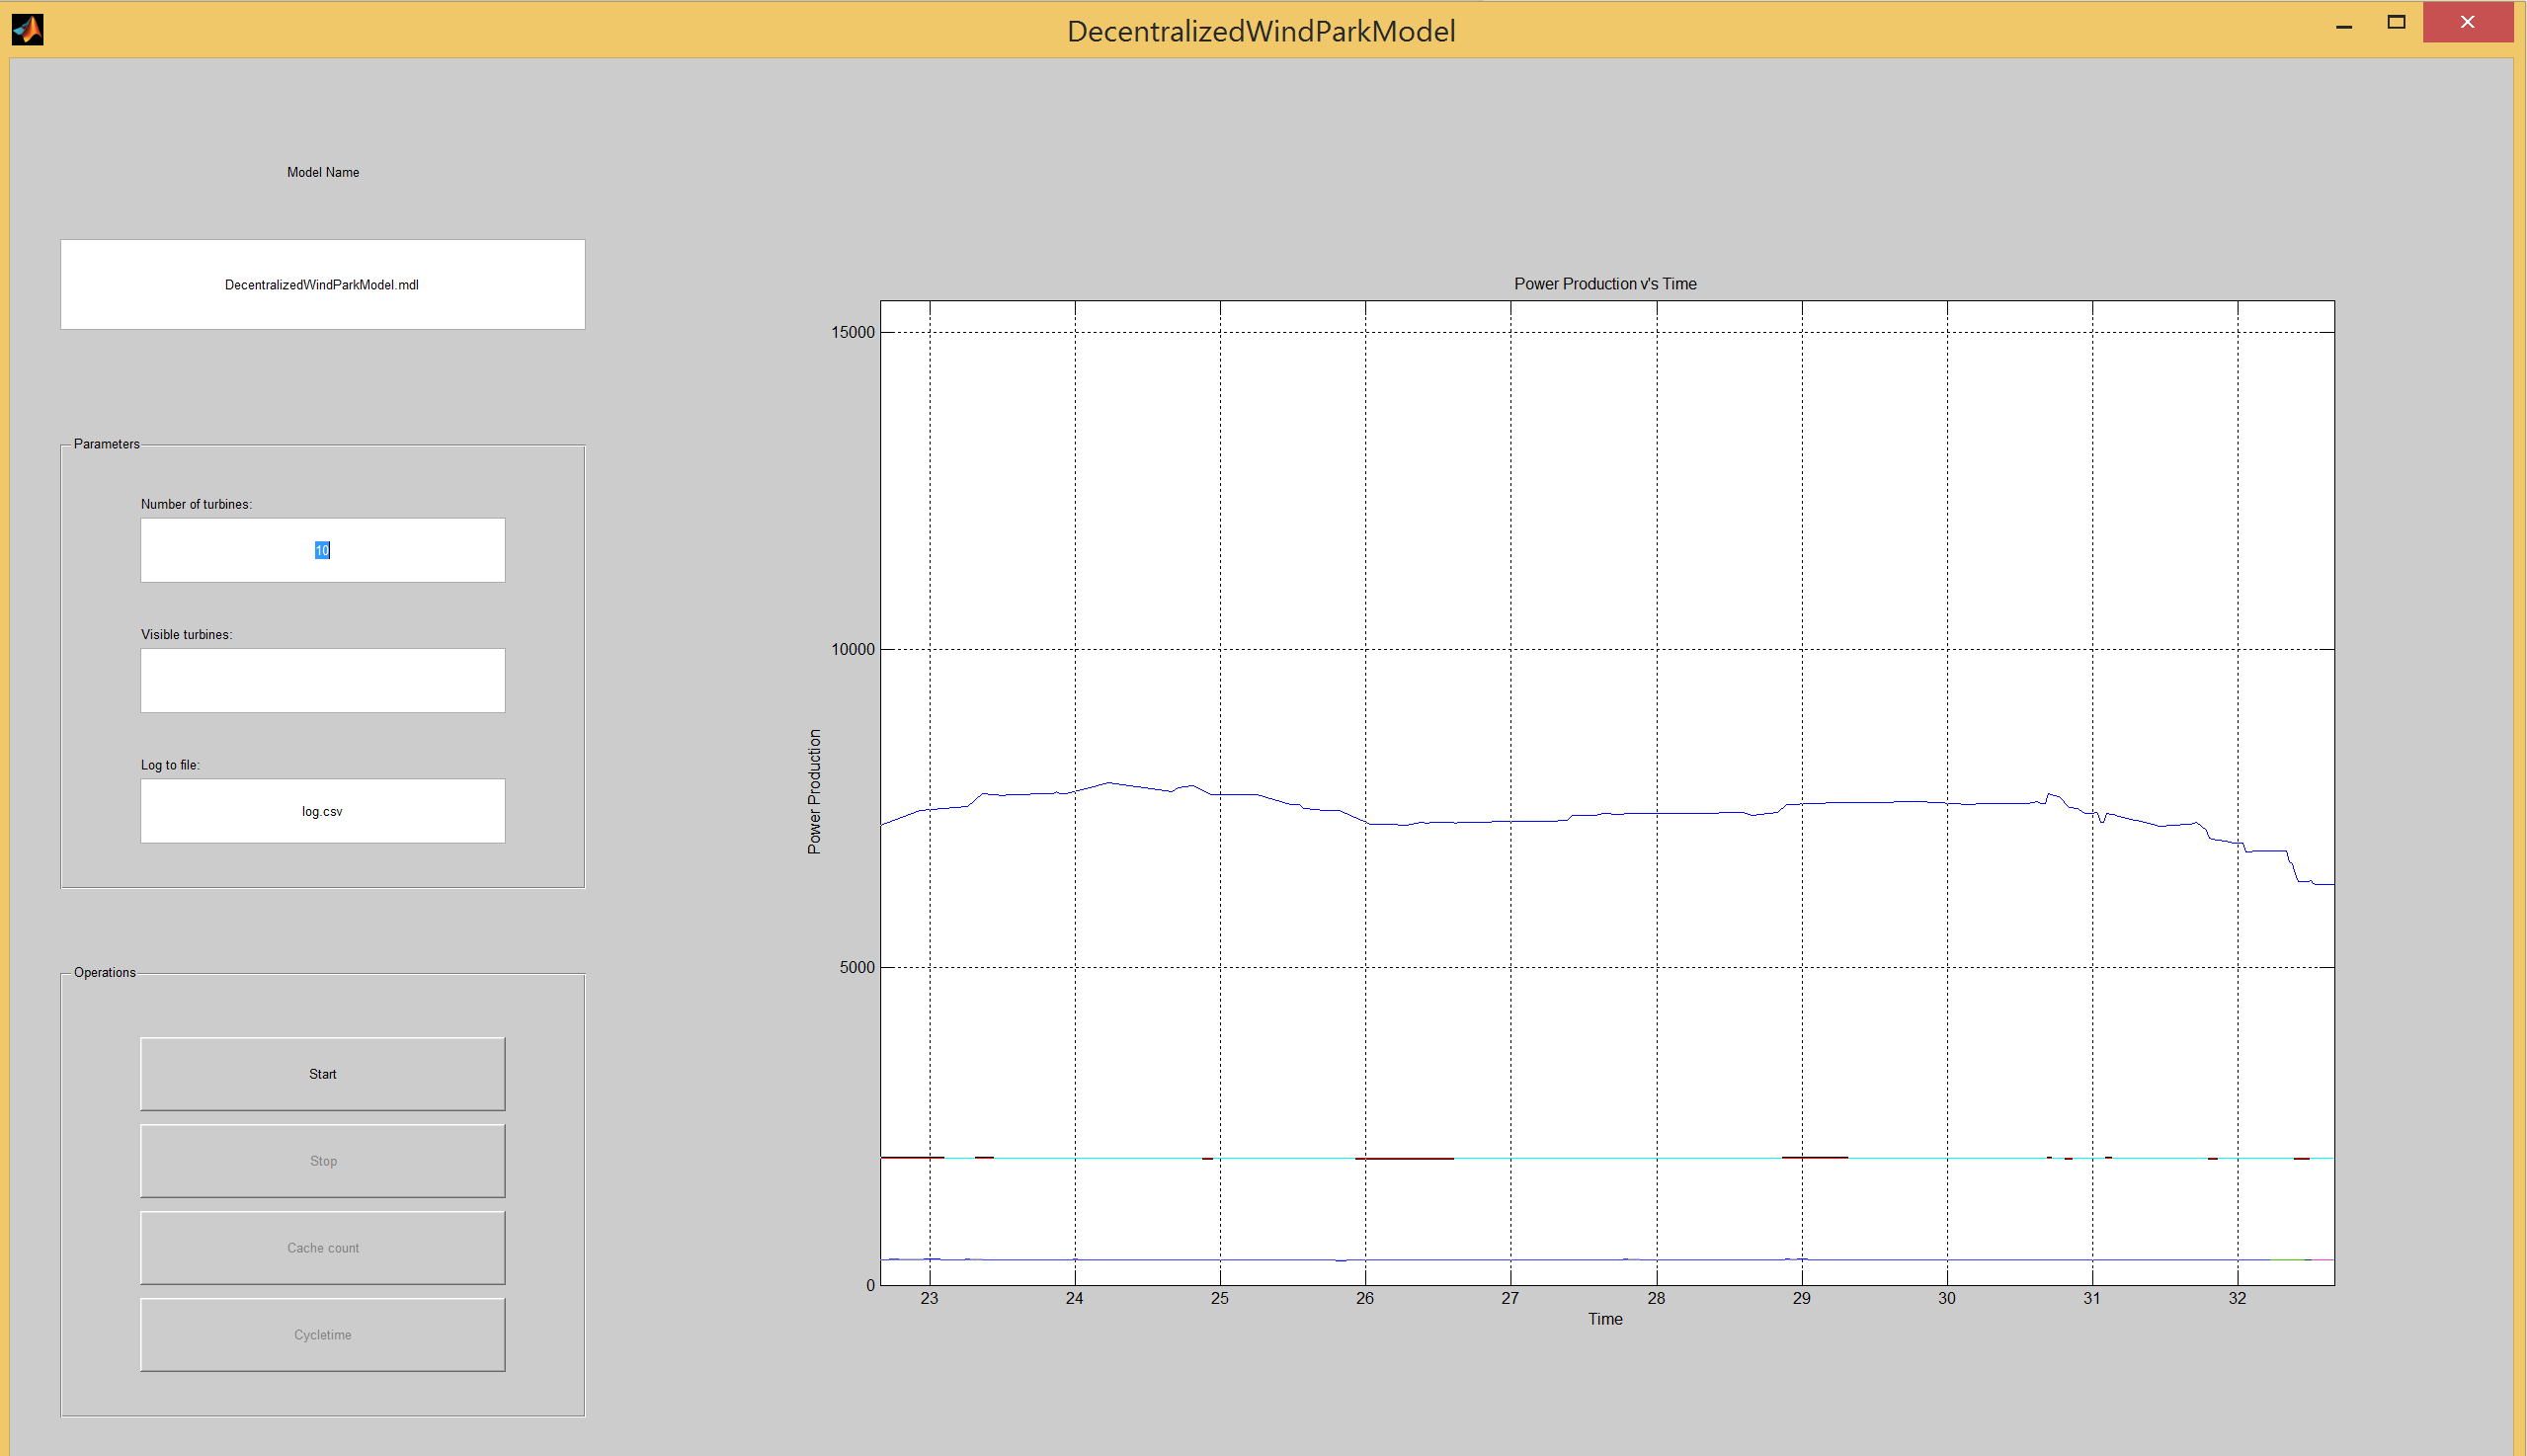
\includegraphics[width=\resultsFigureWidthScale\textwidth]{gui.png} 
	\captionsetup{format=plain,font=footnotesize,labelfont={bf,defaultCapFont},labelsep=quad,singlelinecheck=no}
	\caption[Graphical interface running 10 turbines]{
		\label{fig:graphicalInterface} 
		\footnotesize{%
			Graphical interface running 10 turbines.
		}
	}
\end{figure}

Presented in \cref{fig:graphicalInterface} is a screenshot of the graphical interface made with DDS Blockset for Simulink (described in section \cref{sec:graphicalInterface}). The x-axis show Time in seconds and the y-axis show kW production. The screenshot is taken while the decentralized solution runs 10 turbines.
The global setpoint for power production is illustrated by the red line and is showing a value of just below 5000 kW. The global power production is illustrated by the black line also just below 5000 kW.
The blue line illustrates the maximum available power production for the wind farm which, during this experiment, was above 10000 kW. The lines at the bottom shows values of around 500 kW and they each represents the current power production of each turbine.

\subsection{Discussion}\label{feas:discussion}
The experiment performed to prove whether or not it is feasible to create a decentralized solution that is able to do power regulation, consists of a simple run of the prototype of the decentralized solution. The global setpoint and the global production line match and thus we conclude that we have a working prototype, that can regulate according to the global setpoint. Each turbine is expected to produce $globalSetpoint/nTurbines=5000kW/10=500kW$(see \cref{sec:calculateSetpoints} for detailed description of the regulation algorithm), which they do. The slight deviation (the deviation that makes each turbine produce close to 500kW and not exactly 500kW) is due to the regulation algorithm being inaccurate. For the purpose of this experiment, the fact that the regulation algorithm is inaccurate is acceptable since the regulation algorithm is black box and not the focus of this thesis.

As such it is hard to deduce from a screenshot that the decentralized solution is actually able to perform power regulation, but this experiment in correlation with the rest of the experiments performed in this chapter will show that the prototype is functioning.

In order to decentralize fully decentralize the current Siemens system, decentralization of the Wind Power Supervisor must also be covered. The purpose of the Wind Park Supervisor is to log data from every turbine within the farm and handle external communication. Thus the Wind Park Supervisor consists of two primary features: Data storage and aggregation and external communication. 

Decentralizing the data storage and aggregation onto the turbines requires a horizontally scalable distributed database, which can handle data aggregation. Distributing the database horizontally is important in order to handle datasets larger than the physical storage of one turbine and data aggregation is needed for the case where an external request requires data to be aggregated. To handle this MongoDB~\cite{mongodb} has been identified as the optimal component (as concluded in \cref{sec:databaseStorage} Data Storage). MongoDB supports Sharding for automatic horizontal partitioning of datasets and data aggregation. MongoDB has been chosen based on other parameters related to the problems \ref{PS:Q:Availability} and \cref{PS:Q:Performance}, however to answer the answer the \ref{PS:Q:Feasibility} problem, this functionality is sufficient. 

Handling external communication decentralized means, BLABLA \todo{KRAUSE} has been identified as the optimal component.

\clearpage
\section{\ref{PS:Q:Availability}}

\textit{Can we create a solution where removing one or more nodes from the system at runtime does not cause system failure?}\newline\newline

\noindent To answer whether or not a fully decentralized current Siemens system can handle removing one or more nodes at runtime, the discussion section of this experiment also contains a discussion with regards to the components analyzed in \cref{cha:stateOfTheArt}: \nameref{cha:stateOfTheArt}.\todo{Why the chapter name ref?}

\subsection{Experiments}
The \ref{PS:Q:Availability} problem address if the proposed decentralized solution is able to continue its functions even though nodes are interrupted and removed from the system at runtime.
The proposed decentralized solution should be able to continue maintaining the global setpoint of the wind farm even if some turbines become unavailable, assuming that the needed production capacity is available.

The below experiment is repeated with $N = 1, 5, 10, 15$ failing turbines of 30 running turbines.
%
The experiment has the following procedure:
\begin{enumerate}
	\item Start the system with 30 turbines.
	\item Make sure the system is stable.
	\item Kill N nodes.
\end{enumerate}

Did the system adjust the setpoints for all turbines to maintain the global setpoint?

\subsection{Results}
\label{sec:res:availability}
The plots in \cref{fig:exp:availability_kill15,fig:exp:availability_kill10,fig:exp:availability_kill5,fig:exp:availability_kill1} show how the decentralized solution reacts when killing 1, 5, 10 and 15 turbines. The figures are Matlab screen shots from the graphical interface presented in \cref{sec:graphicalInterface}. The x-axis show time in seconds and the y-axis show kW production. The global setpoint is set to 20,000~kW instead of 2000~kW for the experiment with 1 failing turbine is removed (\cref{fig:exp:availability_kill1}). The global setpoint value for this experiment has been set this high to provide a better visual representation for the case where 1 turbine has crashed. 
% (a change of $globalSetpoint/nTurbines=2,000kW/30=66,6kW$ is harder to see than change of $20,000kW/30=666,6kW$). 
For the remainder of the cases (meaning where 5, 10 and 15 turbines are crashed), the global setpoint is set to 2000~kW.
The turbines are all running with a cycle time of 20 ms throughout this experiment.

\clearpage
\Cref{fig:exp:availability_kill1} shows an increase of production pr. turbine by approximately 20 kW pr. remaining turbines, after a single turbine is crashed. A global setpoint of 20,000kW was set for this test.

\begin{figure} [!h]
	\centering
	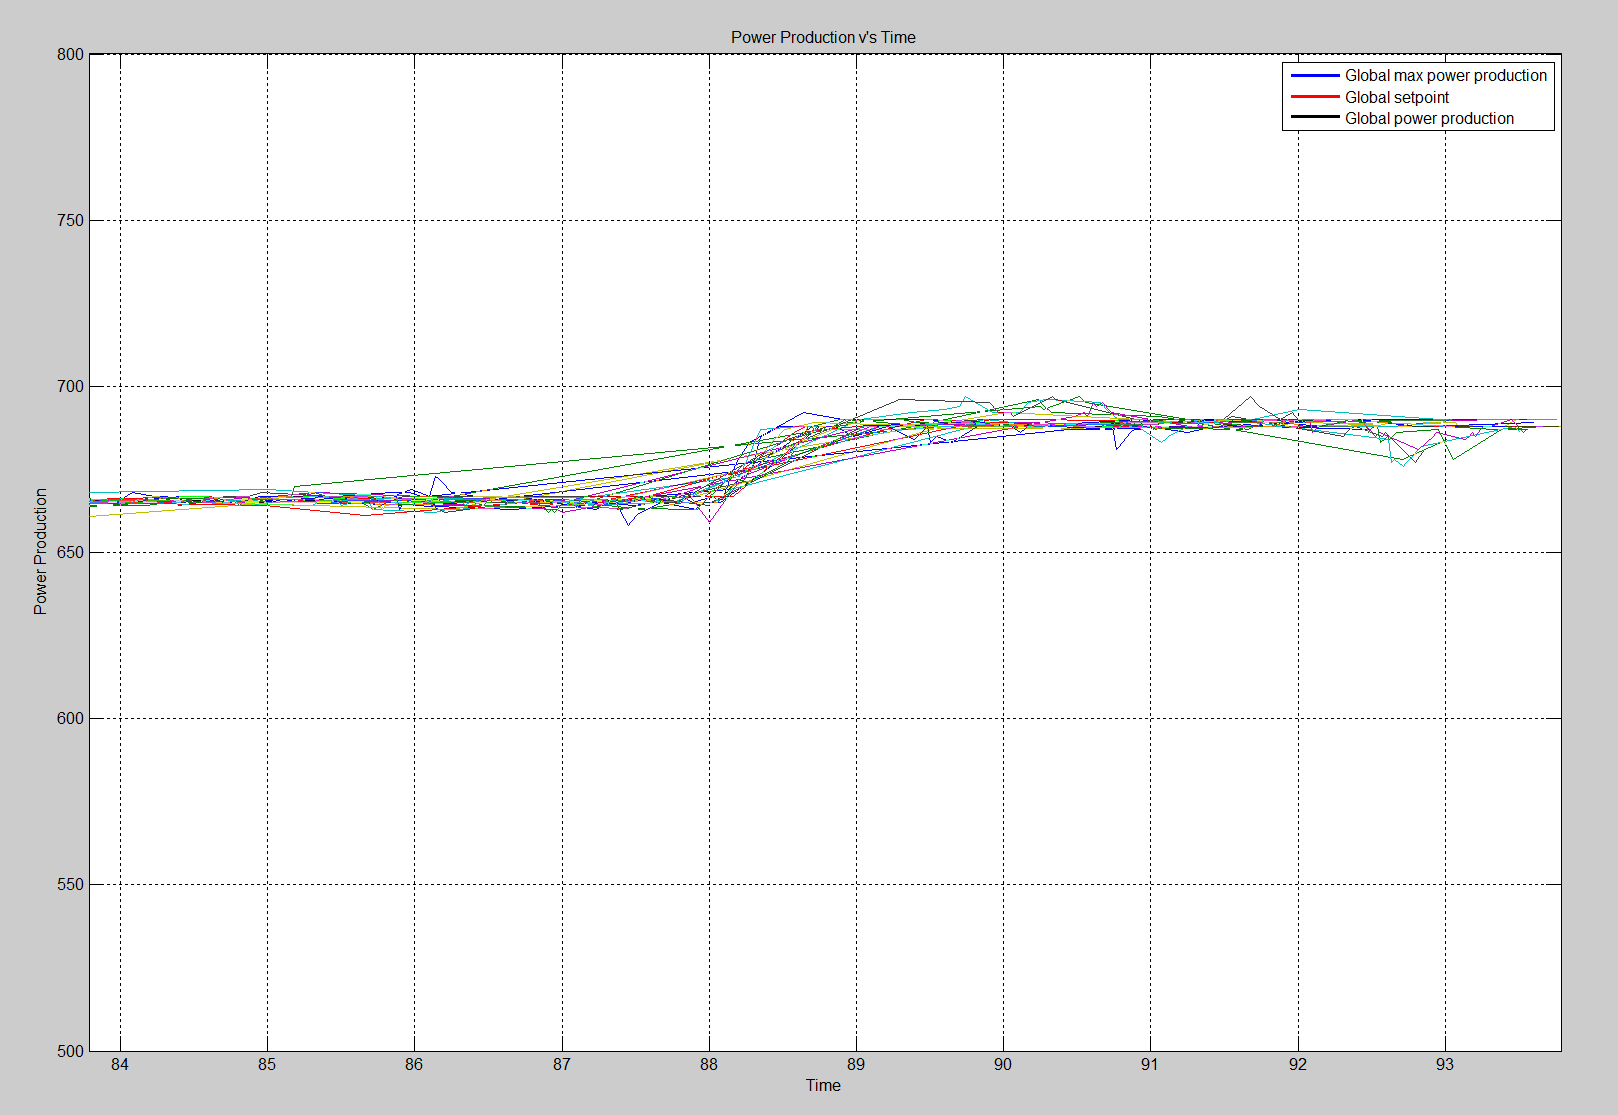
\includegraphics[width=\resultsFigureWidthScale\textwidth]{figures/Results/availabilitytest30-29_setpoint_20000.PNG}
	\caption{Availability test kill 1 out of 30 turbines}
	\label{fig:exp:availability_kill1}
\end{figure}

\Cref{fig:exp:availability_kill5} shows an increase of production pr. turbine by approximately 15 kW pr. remaining turbines, after 5 turbines are crashed. A global setpoint of of 2000kW was set for this test.

\begin{figure} [!h]
	\centering
	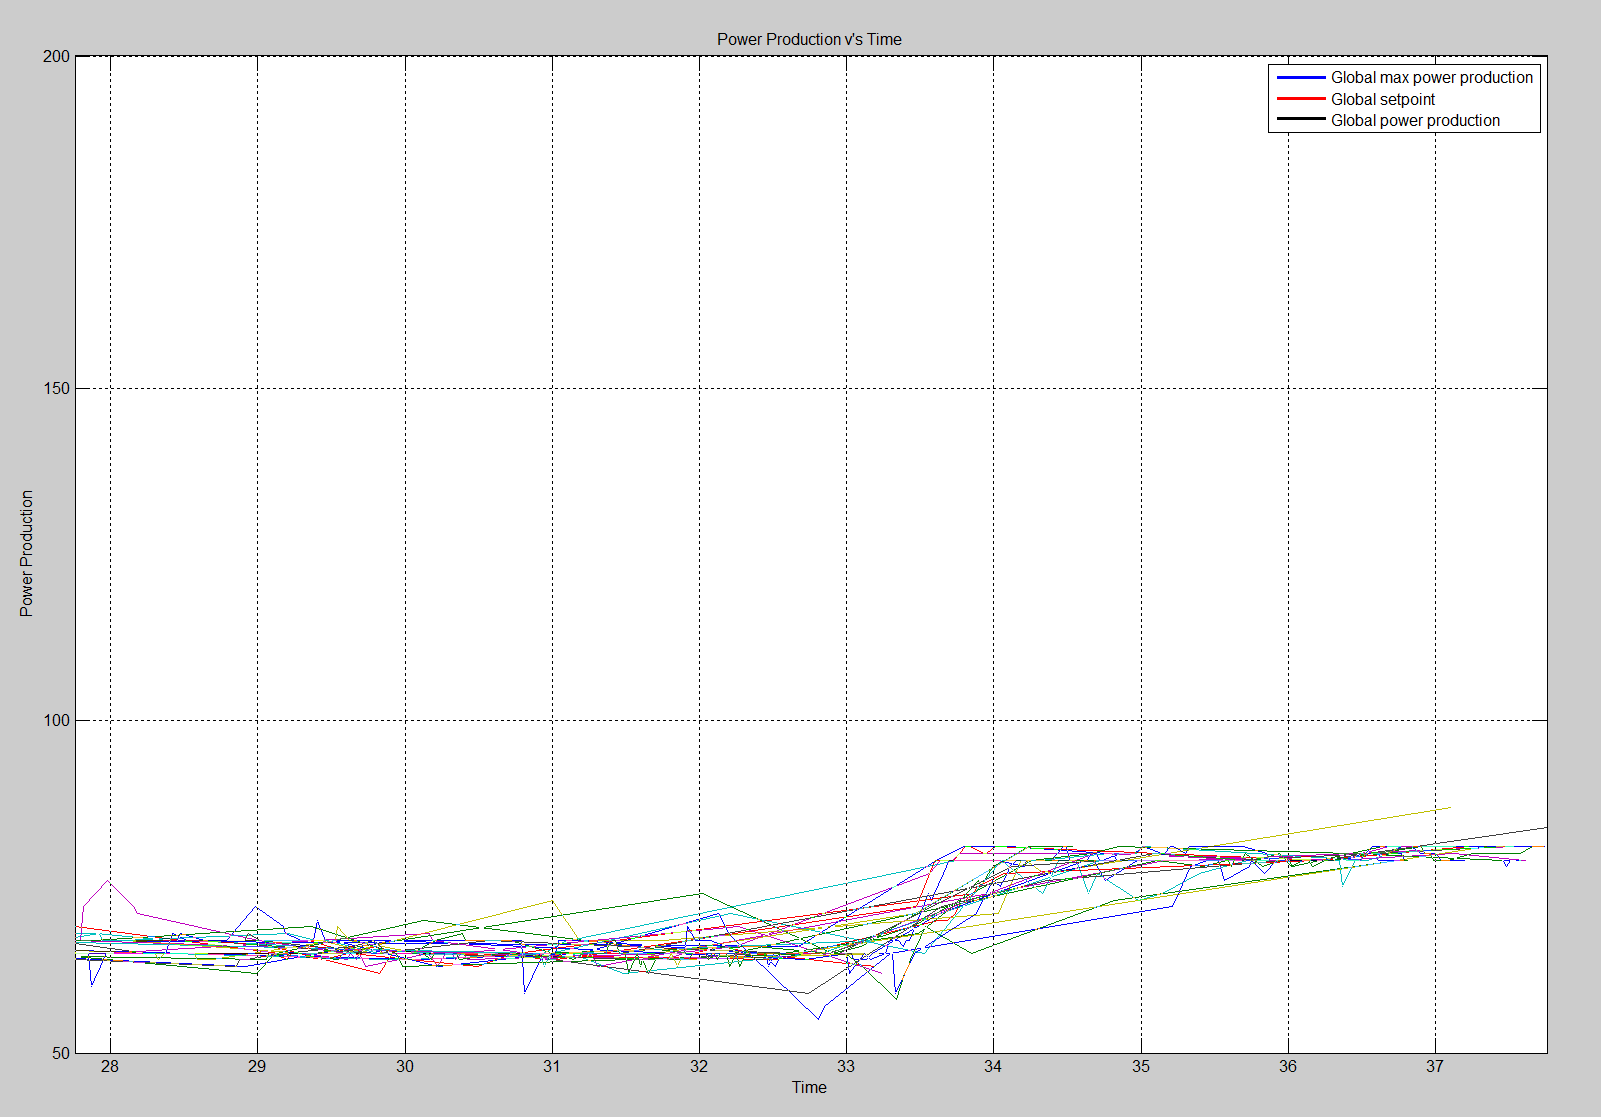
\includegraphics[width=\resultsFigureWidthScale\textwidth]{figures/Results/availabilitytest30-25_setpoint_2000.PNG}
	\caption{Availability test kill 5 out of 30 turbines}
	\label{fig:exp:availability_kill5}
\end{figure}

\FloatBarrier
\Cref{fig:exp:availability_kill10} shows an increase of production pr. turbine by approximately 30 kW pr. remaining turbines, after 10 turbines are crashed. A global setpoint of of 2000kW was set for this test.

\begin{figure}[!h]
	\centering
	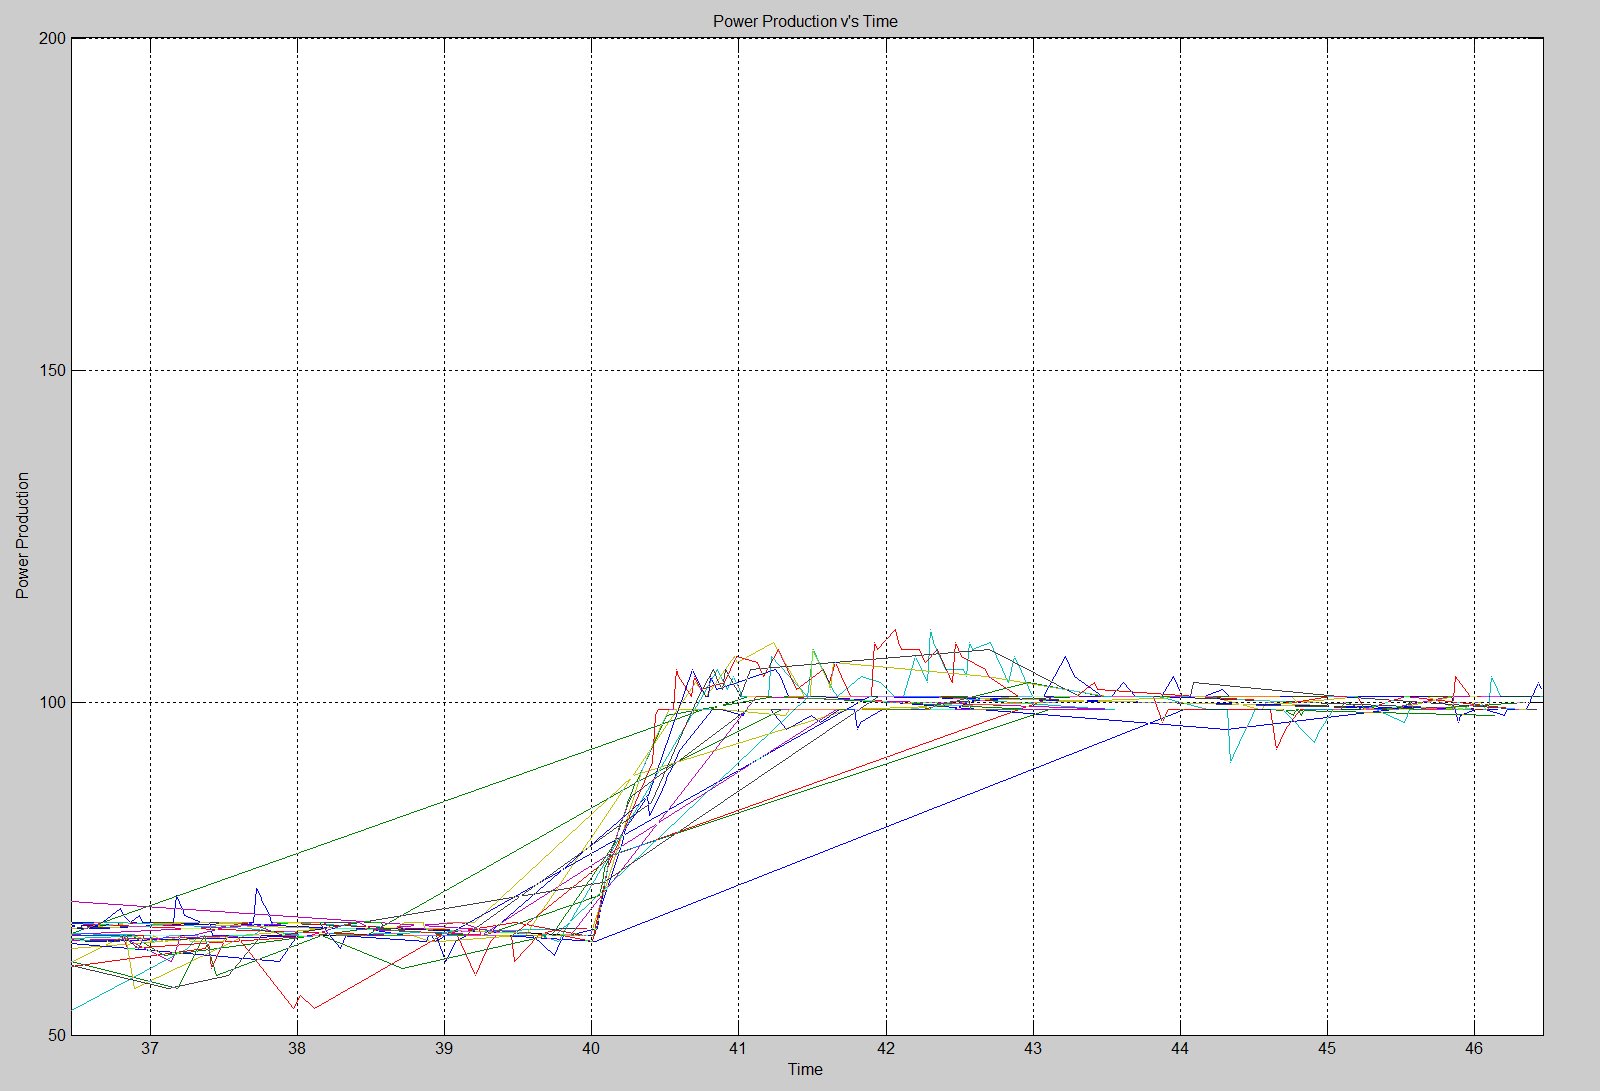
\includegraphics[width=\resultsFigureWidthScale\textwidth]{figures/Results/availabilitytest30-20_setpoint_2000.PNG}
	\caption{Availability test kill 10 out of 30 turbines}
	\label{fig:exp:availability_kill10}
\end{figure}

\FloatBarrier
\Cref{fig:exp:availability_kill15} shows an increase of production pr. turbine by approximately 60 kW pr. remaining turbines, after 15 turbines are crashed. A global setpoint of of 2000kW was set for this test.

\begin{figure}[!h]
	\centering
	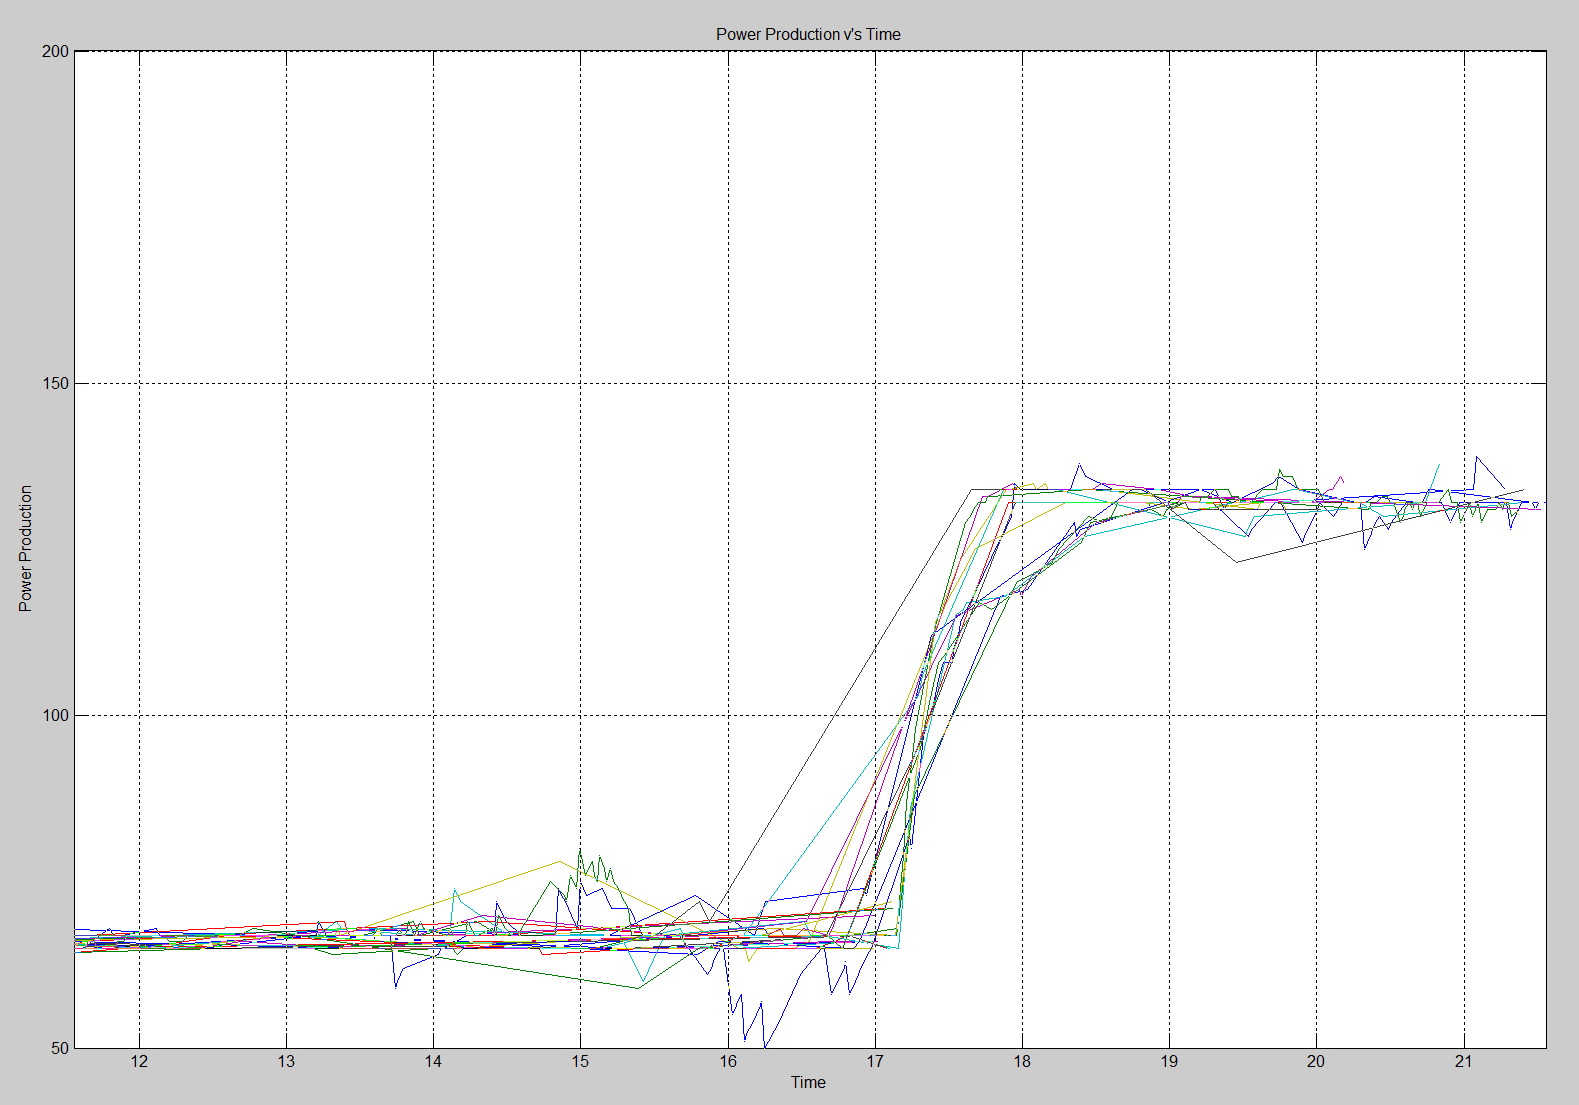
\includegraphics[width=\resultsFigureWidthScale\textwidth]{figures/Results/availabilitytest30-15_setpoint_2000.PNG}
	\caption{Availability test kill 15 out of 30 turbines}
	\label{fig:exp:availability_kill15}
\end{figure}

\FloatBarrier

The 'glitches' in the figures, where the plots shows several seconds between some of the data points, are properly caused by the eventhandler in Matlab handling events from DDS Blockset for Simulink (described in \cref{sec:graphicalInterface}). The eventhandler appears to be neglecting some of the events caused by the publication of turbine states, thus resulting in several seconds time interval between two data points. For the purpose of this experiment we are able to clearly see that it does the regulation, however the time frame is inaccurate.
\todo[inline]{Forklar udfra tråd problemmer istedet for at events bare ikke bliver sent afsted, samme gælder availability GUI afsnittet.}

\subsection{Discussion}
One of the main challenges of highly available is to continue operation in the event of node crashes or loss. As presented in  \cref{fig:exp:availability_kill15,fig:exp:availability_kill10,fig:exp:availability_kill5,fig:exp:availability_kill1} the decentralized solution can handle the loss of turbines. A turbine is considered offline if it does not publish any new data to any other turbines within a 150 ms timespan, defined by the Lifespan QoS parameter of the DataWriter described in \cref{sec:decen:ddsconf}.
This upper limit of 150 ms is chosen because 150 ms is the upper limit of the regulation cycle time in the current Siemens system.
% % % I am HERE Krause
After a turbine crash has been detected the remaining turbines in the wind farm will share the load of the now missing turbines, in order to restore the global power production to the global setpoint.

%The following turbine production increase formula is based on the regulation algorithm definition explained in \cref{sec:calculateSetpoints}.
Let k = the number of turbines crashed, p = production of the crashed turbine, and n = number of remaining turbines. The expected increase of production pr. turbine when k turbines have crashed, is denoted as: 
$$Production~increase~per~turbine = \frac{\sum\limits_{i=1}^k(p)}{n}$$

Thus the expected production increase for the case where a single turbine is crashed (\cref{fig:exp:availability_kill1}) is: $$\frac{\sum\limits_{i=1}^1(666,6kW)}{29}\approx23kW$$

Hence for the rest of the cases (note that the global setpoint for these cases are 2000kW, thus the production of each turbine is 66,6 kW as apposed to 666,6 kW for the case where one turbine was crashed):
\newline\newline
\noindent5 turbines crashed (\cref{fig:exp:availability_kill5}) $$\frac{\sum\limits_{i=1}^5(66,6kW)}{25}\approx13kW$$

\noindent10 turbines crashed (\cref{fig:exp:availability_kill10}) $$\frac{\sum\limits_{i=1}^{10}(66,6kW)}{20}\approx33kW$$

\noindent15 turbines crashed (\cref{fig:exp:availability_kill15}) $$\frac{\sum\limits_{i=1}^{15}(66,6kW)}{15}\approx67kW$$

These expected values matches the increased productions shown in \cref{fig:exp:availability_kill5,fig:exp:availability_kill10,fig:exp:availability_kill15}. The glitches \todo{Anden brug af glitches} in the figures are caused by the simulated turbine data and is therefore accepted for the purpose of this experiment. Thus we conclude that the remaining turbines share the extra load between themselves and power production continues after turbine crashes.
This means removing one or multiple turbines from the system does not impede the regulation of the wind farm.

%The time it takes the decentralized solution to detect a turbine loss and recover power production is dependent on the following parameters:
%
%\begin{itemize}
%	\item Time of turbine loss detection, which is defined by the History QoS to 150 ms, $I$.
%	\item Time between regulation cycles, in the test cases presented in \cref{sec:res:availability} the time is set to 20 ms, $S$.
%	\item Time of calulation of a new setpoint, $C$.
%	\item Time for the turbine to regulate power production according to the new setpoint. In the turbines this process is simulated with a simple regulation that may take several regulation cycles to complete $R$.
%\end{itemize}
%
%Thus the time for recovery of the power production when a turbine failure occurs can be calculated as $T = I + S + C + R$ which translates to $150 ms + 20 ms + C + R = 170 + C + R ms$. This time can be reduced by lowering the time it takes to detect a turbine is offline which increases the likelihood of detecting a delayed turbine as offline, or by lowering the time between regulation cycles which increases the likelihood of cache reads.

The time it takes for the turbines to regulate according to crashed turbines are of course an important factor.
\todo{Expalin why}
However since we are using an arbitrary regulation algorithm and turbine simulations, we cannot conclude anything with regards to this subject.

% The only thing we can conclude is that the turbines regulate according to multiple crashed turbines relatively fast, meaning that the time it takes for the turbines to regulate according to one or more crashes happens within an acceptable timeframe of 1 to 4 seconds. 

When it comes to availability for the a potential decentralized wind farm, handling the communication for the regulation algorithm run by the Park Pilot is only one part of the picture. Availability for the decentralized Wind Park Supervisor, which handles external communication and data storage and aggregation, must also be addressed. 

To ensure available data storage, the problem of data loss when a turbine is unresponsive must be addressed. A turbine has several control and measurement points which are continually logged to a local data store. Should a turbine break down, the local data may be destroyed with the turbine. This sets special requirements to the component handling data storage. In \cref{sec:databaseStorage} the requirements to the data storage component is described and MongoDB was identified as the best choice to solve the availability problem related to data storage. MongoDB is capable of replication of data between turbines, such that data is still available should a turbine crash occur. As well as replication MongoDB provides sharding of a database, which enables a global database to be stored across multiple nodes. Replication and sharding can be combined such that no single node contains all global data. This is needed to prevent single point of failures. 

Sharding is needed in order to make the database scale horizontally. Thus in order to make a system where removing nodes from the system does not cause system failure, replication of each shard is needed. However, replication of shards only solve the problem to some extent, since removing all replicated copies of a single shard renders the shard unavailable, thus rendering a part of the database unavailable. To prevent this from happening, an appropriate amount of turbines must be allocated per shard. This to heighten the availability of the wind farm, increasing the number of turbines per shard, however this also increases the amount of data storage used for the database, since it causes duplicated data. Thus increasing availability of the system is at the cost of data storage used per turbine.

Making the decentralized solution robust and able to handle the loss of turbines with regards to internal communication, regulation of power production, external communication and data storage increases the overall availability of the wind farm. %With MongoDB chosen for data storage and BLABLA chosen for resource management, we conclude availability for the case where removing a few amount of nodes does not cause system failure is definitely feasible. Increasing the number of turbine crashes the system needs to be able to handle increases the disk storage needed on each turbine.

To handle communication with the outside world we use a load balancer as a single external entry point, 
however it must be prevented that it becomes a single point of failure.
To prevent this we are using a load balancer with automatic fail over, in section \cref{cha:resourceManagement} such a system described.
It continuously keep the active connections information synchronized between active and backup nodes and uses heartbeat monitoring to detect a node crash.
The load balancer setup helps solve the \ref{PS:Q:Availability} problem.

\clearpage

\section{\ref{PS:Q:Performance}}

\textit{Can we create a solution that scales such that the number of turbines does not impact the regulation cycle time?}

\subsection{Experimenit}
\label{sec:Exper:perfom}

%Scalability is by Bondi\cite{Bondi:2000:CSI:350391.350432} defined as \textit{the systems ability to accommodate an increasing number of elements or objects, to process growing volumes of work gracefully, and/or to be susceptible to enlargement}.

The \ref{PS:Q:Performance} question asks if the proposed decentralized solution is able to keep a constant regulation cycle time independent from the number of turbines. This problem operates in a 3-dimensional space with cycle time (ms), number of cache reads and number of turbines as parameters. To study the correlation between the parameters, we isolate two parameters by making the third constant.

Thus to fully address \ref{PS:Q:Performance} this experiment has been divided into two experiments:
 
\begin{description}
	\item[Experiment 1] aims to investigate the anti-correlation between the implemented sleep time of the regulation cycle and the number of cache reads for the decentralized system. This is relevant because changing the sleep time is expected to impact the number of cache reads, since an increase in sleep time increases the time Connext has to overwrite received states, thus decreasing the number of cache reads (as explained in \cref{sec:cachereads}: Cache reads). Thus the constant for this is experiment is the number of turbines.
	\item[Experiment 2] aims to investigate the impact on the regulation cycle time and the number of cache reads when increasing the number of turbines in the decentralized solution, and thus answer the \ref{PS:Q:Performance} problem. The constant for this experiment is the sleep time.
\end{description}


\subsection{Experiment 1: How sleep time impacts the regulation cycle time and the number of cache reads}
\label{subsec:Exper:perfom:1}
The purpose of this experiment is to show how the sleep time affects the number of cache reads and the regulation cycle time for the decentralized solution (see \cref{sec:cachereads} for cache reads description).  
The experiment is performed with cycle time t=\testCycletimeNumbers.  

The following procedure is used each time the experiment is performed:
\begin{enumerate}
	\item Start the system with a cycle time of t ms and 21 turbines.
	\item Make sure the system is stable.
	\item Start logging the regulation cycle time and the number of cache reads.
	\item Stop logging when 1000 data points are reached.
\end{enumerate}

\subsection{Experiment 2: How the number of turbines impacts the regulation cycle time and the number of cache reads}
\label{subsec:Exper:perfom:2}
The purpose of this experiment is to answer the \ref{PS:Q:Performance} problem, by showing how the number of turbines affects the regulation cycle time for the decentralized solution. To complete the picture we also investigate how the number of turbines affects the cache reads, since an expected side effect of increasing the number of turbines also increases the number of cache reads as described in \cref{sec:cachereads}.

The experiments are performed with n=\testTurbineNumbers ~turbines. The sleep time is set to 20 ms and is constant for this experiment.

The test system is expected to be running only one instance in a real life implementation, therefore the machine logging the data will only run one instance and the supporting machines will run the rest generating system load.

The following procedure is used each time the experiment is performed:
\begin{enumerate}
	\item Start the system with N turbines.
	\item Make sure the system is stable.
	\item Start logging the reported regulation run time and the number of cache reads.
	\item Stop logging when 1000 data points are reached.
\end{enumerate}


\subsection{Results}

\label{sec:exp:performance}
The cycle regulation time is defined as the difference between the receive timestamp of the oldest turbine state(tOldestState) received and the timestamp sampled right after, a new turbine state has been sent (tSent) (as illustrated on \cref{fig:timingDecentral}):

$$regulation~cycle~time=tSent-tOldestState$$

\begin{figure}[b]
	

{ %The brackets issolate the enviroment

\makeatletter
\ifcsname c@wavenum\endcsname %Only create one counter
\else
	\newcounter{wavenum}
\fi
\makeatother

\newcommand*{\bitvector}[3]{
  \draw[fill=#3] (t_cur) -- ++( .1, .3) -- ++(#2-.2,0) -- ++(.1, -.3)
                         -- ++(-.1,-.3) -- ++(.2-#2,0) -- cycle;
  \path (t_cur) -- node[anchor=mid](textNode) {#1} ++(#2,0) node[time] (t_cur) {};
}

% \known{val}{length}
\newcommand*{\known}[2]{
    \bitvector{#1}{#2}{white}
}

% \unknown{length}
\newcommand*{\unknown}[2]{
    \bitvector{#1}{#2}{black!20}
}

% \nextwave{name}
\newcommand{\nextwave}[1]{
  %\path (0,\value{wavenum}) node[left] {#1} node[time] (t_cur) {};
  \path (0,\value{wavenum}) node[time] (t_cur) {};
  \addtocounter{wavenum}{-1}
}

%\newcommand{\timeSpanLabel}{
%	\node (CycleTimeLabel) [rectangle, above = 0.25cm of textNode, inner sep=10pt] {CycleTime};	  
%}

\newcommand{\timeSpanLabel}{
	\node (CycleTimeLabel) [rectangle, above = 1.02cm of t_cur, inner sep=0pt] {Regulation cycle time};
}

\newcommand{\timeSpanA}{
	\node (t_timeSpanA) [point, above = 0 of t_cur] {};	  
}

\newcommand{\timeSpanB}{
	\node (t_timeSpanB) [point, above =0 of t_cur] {};
	
	\graph[use existing nodes]{
		t_timeSpanA --[time span=1cm] CycleTimeLabel;
		CycleTimeLabel.south --[time span=-0.24cm] t_timeSpanB;
	}; 
	
}

%%% End of timing.sty

\begin{tikzpicture}[
	point/.style={inner sep=0pt}, %circle,minimum size=2pt,fill=red},
	draw=black, 
	yscale=.8,
	xscale=1,
	hv path/.style={to path={-| (\tikztotarget)}},
	vh path/.style={to path={|- (\tikztotarget)}},
	skip loop v/.style={to path={-- ++(#1,0) |- (\tikztotarget)}},		
	skip loop h/.style={to path={-- ++(0,#1) -| (\tikztotarget)}},
	time span/.style={to path={-- ++(0,#1) -| (\tikztotarget)}},
	graphs/every graph/.style={edges=rounded corners}	
]
	
\tikzstyle{time}=[coordinate]
\setlength{\unitlength}{1cm}
\setcounter{wavenum}{0}

	\nextwave{} \timeSpanA \unknown{readStates}{3} \unknown{calculate}{3} \timeSpanLabel \unknown{setSetpoint}{3} \unknown{sendState}{3} \timeSpanB \known{wait}{2}
	\nextwave{} \known{reciveStates}{14}
\end{tikzpicture}
}

	\caption{Decentralized regulation time}
	\label{fig:timingDecentral}
\end{figure}

The timestamp of the oldest turbine state is used to include network traffic in the regulation cycle time, as opposed to just sampling the time locally.

We use the following box plot type (for \cref{fig:exp:decen:sleep} and \cref{fig:exp:decen:turbines}): The central mark is the median, the edges of the box are the 25th and 75th percentiles, the whiskers extend to the most extreme data points not considered outliers, and outliers are plotted individually. The whisker length is denoted as 1.5 IQR. 

The red line plots the medians.

\subsubsection{\nameref{subsec:Exper:perfom:1}}

\begin{figure}[h!]
	\centering
	\begin{tikzpicture}
\begin{axis}
[
width=\resultsFigureWidthScale\textwidth,
axis y line*=left,
xlabel=Sleeptime (ms),
ylabel=Regulation cycle time (ms),
ymin = 0,
xtick={1, 2, 3, 4, 5, 6, 7, 8, 9},
xticklabels={10, 15, 20, 25, 30, 35, 40, 45, 50},
boxplot/draw direction=y
]

%% /home/stefan/work/TestResults/Test6_Decentralized_12-7-2014_1327/nCycleTime/DecentralizedLog1.csv
\buildBoxPlot{10.578002}{15.286001}{9.942}{148.911}{0.415002}

%% /home/stefan/work/TestResults/Test6_Decentralized_12-7-2014_1327/nCycleTime/DecentralizedLog2.csv
\buildBoxPlot{15.026002}{15.383002}{14.312002}{26.729001}{1.379}

%% /home/stefan/work/TestResults/Test6_Decentralized_12-7-2014_1327/nCycleTime/DecentralizedLog3.csv
\buildBoxPlot{19.926}{20.380001}{18.979001}{29.932002}{0.435}

%% /home/stefan/work/TestResults/Test6_Decentralized_12-7-2014_1327/nCycleTime/DecentralizedLog4.csv
\buildBoxPlot{25.079001}{25.322}{24.637001}{32.794001}{12.225002}

%% /home/stefan/work/TestResults/Test6_Decentralized_12-7-2014_1327/nCycleTime/DecentralizedLog5.csv
\buildBoxPlot{30.099}{30.363}{29.565001}{42.436}{4.466}

%% /home/stefan/work/TestResults/Test6_Decentralized_12-7-2014_1327/nCycleTime/DecentralizedLog6.csv
\buildBoxPlot{35.153001}{35.328002}{34.853001}{45.836001}{10.347}

%% /home/stefan/work/TestResults/Test6_Decentralized_12-7-2014_1327/nCycleTime/DecentralizedLog7.csv
\buildBoxPlot{40.157001}{40.434001}{39.626}{58.338001}{6.398001}

%% /home/stefan/work/TestResults/Test6_Decentralized_12-7-2014_1327/nCycleTime/DecentralizedLog8.csv
\buildBoxPlot{45.185}{45.330001}{44.928002}{50.089}{29.313}

%% /home/stefan/work/TestResults/Test6_Decentralized_12-7-2014_1327/nCycleTime/DecentralizedLog9.csv
\buildBoxPlot{49.958002}{50.391001}{49.019}{64.611002}{4.846}


\addplot[thick, red!70] coordinates {
	(1 ,10.578002)
	(2 ,15.026002)
	(3 ,19.926)
	(4 ,25.079001)
	(5 ,30.099)
	(6 ,35.153001)
	(7 ,40.157001)
	(8 ,45.185)
	(9 ,49.958002)
	
};

\end{axis}
\end{tikzpicture}

	\caption{Decentralized solution with variable wait time cycle time experiment}
	\label{fig:exp:decen:sleep}
\end{figure}

\Cref{fig:exp:decen:sleep} show that the regulation cycle times and wait times are linearly dependent on each other. The maximum value with wait time 10 is outside the boundaries of the plot but is calculated to 148.91 ms. The upper and lower quartile are close together the exception is the 10 ms wait time sample. The maximum being the 20 ms wait time having a difference of 1.401 ms between upper and lower quantile and the minimum being 45 ms wait time with a difference of 0.402 ms. The maximum values again with the exception of the 10 ms wait time sample follow the median values, the minimum values are able to reach low regulation cycle times much lower than the wait time used in the experiment.

\begin{figure}[h!]
	\centering
	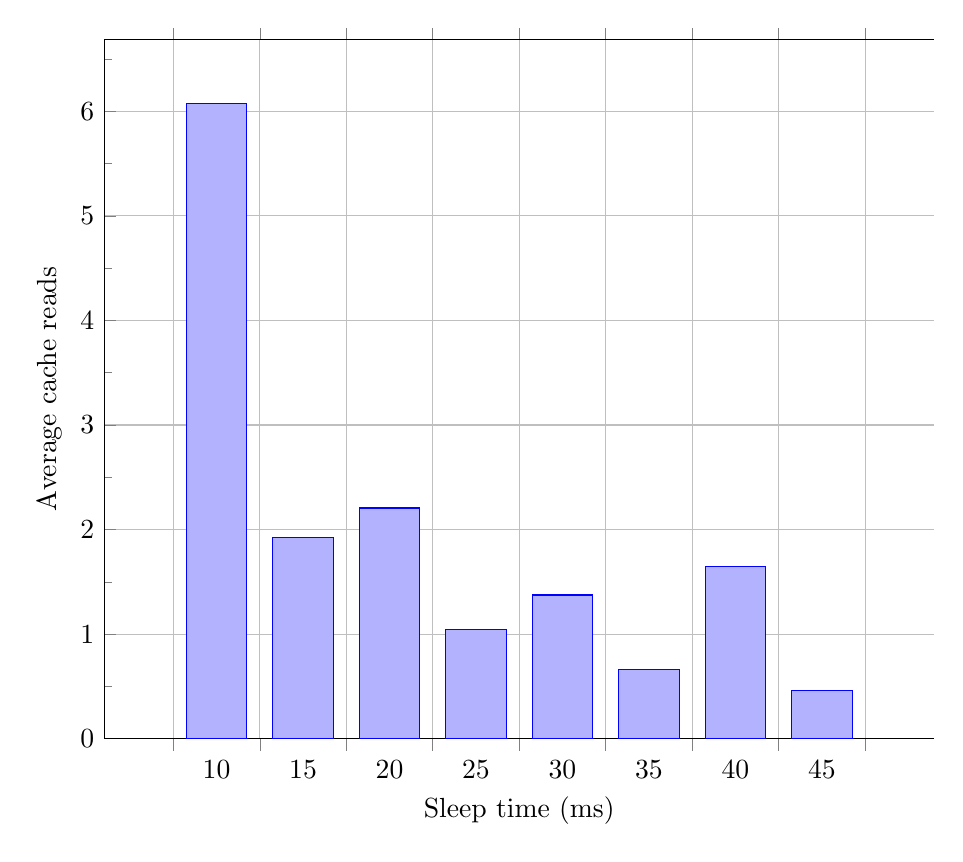
\begin{tikzpicture}
\begin{axis}
[
width=\resultsPlotWidthScale\textwidth,
axis y line*=left,
xlabel=Sleep time (ms),
ymin = 0,
%xmin = 0,
ylabel=Average cache reads,
%xtick={1, 2, 3, 4, 5, 6, 7, 8, 9},
%xticklabels={10, 15, 20, 25, 30, 35, 40, 45, 50},
%boxplot/draw direction=y,
%grid=both,
%ymajorgrids=true,
%yminorgrids=true,
ybar interval=0.7,
ymajorgrids=true,
%yminorgrids=true,
minor y tick num=1
%minor tick num=1
]
%\buildBoxPlot[black]{0}{0}{0}{0}{0}
%\buildBoxPlot[black]{0}{0}{0}{0}{0}
%\buildBoxPlot[black]{0}{0}{0}{0}{0}
%\buildBoxPlot[black]{0}{0}{0}{0}{0}
%\buildBoxPlot[black]{0}{0}{0}{0}{0}
%\buildBoxPlot[black]{0}{0}{0}{0}{0}
%\buildBoxPlot[black]{0}{0}{0}{0}{0}
%\buildBoxPlot[black]{0}{0}{0}{0}{0}
%\buildBoxPlot[black]{0}{0}{0}{0}{0}
\addplot coordinates {
	(10 ,6.076278918444858)
	(15 ,1.9250837336102817)
	(20 ,2.206446850393701)
	(25 ,1.044688862465319)
	(30 ,1.3747593094220163)
	(35 ,0.661782154722354)
	(40 ,1.6464805561590268)
	(45 ,0.46317152740208856)
	(50 ,1.858914282814271)
};

%matlab info
%     General model:
%     f(x) = (a/(x+b))+ c
%     Coefficients (with 95% confidence bounds):
%     a =       7.017  (-8.781, 22.82)
%     b =      -8.622  (-11.55, -5.697)
%     c =      0.9821  (0.01249, 1.952)
     
%\addplot[
%red,
%domain=10:50,
%samples=201,
%]
%{(7.017/(x-8.622))+ 0.9821};

\end{axis}
\end{tikzpicture}
	\caption{Decentralized solution with variable wait time cache reads experiment}
	\label{fig:exp:decen:sleep-cache}
\end{figure}

\Cref{fig:exp:decen:sleep-cache} show the average cache reads of the experiment.
A cache read only happens in the decentralized solution and is a consequence of the separation of receiving data in a separate thread.
The cache read happens if the wait time elapses before all turbine instances have responded with state information. The Number dos not include information of if the same turbine instance state has been read from cache multiple times.
The number of cache reads is declining. 
%, a fitted function of the plot has been put on top (red), the plot is in Matlab fitted against the function $\dfrac{a}{x + b} + c$.

\clearpage
\subsubsection{\nameref{subsec:Exper:perfom:2}}
The plots in this section relates to the second part of the \nameref{sec:Exper:perfom} experiment. In this graph the regulation cycle time is plotted against a variating number of turbines.

\begin{figure}[h!]
	\centering
	\begin{tikzpicture}
\begin{axis}
[
width=\textwidth,
axis y line*=left,
xlabel=Number of turbines,
ylabel=Regulation cycle time (ms),
ymin = 0,
xtick={1, 2, 3, 4, 5, 6, 7, 8, 9, 10, 11, 12, 13, 14, 15, 16, 17, 18, 19, 20},
xticklabels={5, 10, 15, 20, 25, 30, 35, 40, 45, 50, 55, 60, 65, 70, 75, 80, 85, 90, 95, 100},
boxplot/draw direction=y
]

%% /home/stefan/work/TestResults/Test5_Decentralized_success_12-4-2014_2100/nTurbines/DecentralizedLog0.csv
\buildBoxPlot{19.526002}{20.412002}{15.272001}{26.620001}{0.282}

%% /home/stefan/work/TestResults/Test5_Decentralized_success_12-4-2014_2100/nTurbines/DecentralizedLog1.csv
\buildBoxPlot{20.257002}{20.365001}{20.158001}{24.403002}{0.828002}

%% /home/stefan/work/TestResults/Test5_Decentralized_success_12-4-2014_2100/nTurbines/DecentralizedLog2.csv
\buildBoxPlot{20.221001}{20.311002}{20.126002}{24.641001}{3.778}

%% /home/stefan/work/TestResults/Test5_Decentralized_success_12-4-2014_2100/nTurbines/DecentralizedLog3.csv
\buildBoxPlot{20.203002}{20.321002}{20.066}{24.962}{0.246002}

%% /home/stefan/work/TestResults/Test5_Decentralized_success_12-4-2014_2100/nTurbines/DecentralizedLog4.csv
\buildBoxPlot{20.174001}{20.343}{19.946}{25.983002}{0.273002}

%% /home/stefan/work/TestResults/Test5_Decentralized_success_12-4-2014_2100/nTurbines/DecentralizedLog5.csv
\buildBoxPlot{20.190001}{20.286002}{20.051}{24.771001}{10.959001}

%% /home/stefan/work/TestResults/Test5_Decentralized_success_12-4-2014_2100/nTurbines/DecentralizedLog6.csv
\buildBoxPlot{20.079}{20.391001}{19.563001}{27.503001}{0.371002}

%% /home/stefan/work/TestResults/Test5_Decentralized_success_12-4-2014_2100/nTurbines/DecentralizedLog7.csv
\buildBoxPlot{20.176}{20.303001}{19.965}{30.63}{9.225}

%% /home/stefan/work/TestResults/Test5_Decentralized_success_12-4-2014_2100/nTurbines/DecentralizedLog8.csv
\buildBoxPlot{19.998}{20.351001}{19.215}{30.385002}{0.543001}

%% /home/stefan/work/TestResults/Test5_Decentralized_success_12-4-2014_2100/nTurbines/DecentralizedLog9.csv
\buildBoxPlot{20.008}{20.384001}{19.068001}{29.380001}{4.096002}

%% /home/stefan/work/TestResults/Test5_Decentralized_success_12-4-2014_2100/nTurbines/DecentralizedLog10.csv
\buildBoxPlot{19.902002}{20.353}{18.909001}{33.447001}{2.831002}

%% /home/stefan/work/TestResults/Test5_Decentralized_success_12-4-2014_2100/nTurbines/DecentralizedLog11.csv
\buildBoxPlot{19.937001}{20.373}{18.991001}{33.877001}{1.672002}

%% /home/stefan/work/TestResults/Test5_Decentralized_success_12-4-2014_2100/nTurbines/DecentralizedLog12.csv
\buildBoxPlot{20.056}{20.415001}{19.421002}{40.952001}{0.923001}

%% /home/stefan/work/TestResults/Test5_Decentralized_success_12-4-2014_2100/nTurbines/DecentralizedLog13.csv
\buildBoxPlot{20.215}{21.471}{19.378}{151.296001}{0.528001}

%% /home/stefan/work/TestResults/Test5_Decentralized_success_12-4-2014_2100/nTurbines/DecentralizedLog14.csv
\buildBoxPlot{19.920001}{20.535002}{18.897001}{53.699}{0.768}

%% /home/stefan/work/TestResults/Test5_Decentralized_success_12-4-2014_2100/nTurbines/DecentralizedLog15.csv
\buildBoxPlot{20.129002}{21.354002}{18.846002}{69.145001}{0.589001}

%% /home/stefan/work/TestResults/Test5_Decentralized_success_12-4-2014_2100/nTurbines/DecentralizedLog16.csv
\buildBoxPlot{20.189001}{22.247}{18.578001}{89.297001}{0.707}

%% /home/stefan/work/TestResults/Test5_Decentralized_success_12-4-2014_2100/nTurbines/DecentralizedLog17.csv
\buildBoxPlot{20.902001}{25.559001}{18.828}{142.836}{0.615001}

%% /home/stefan/work/TestResults/Test5_Decentralized_success_12-4-2014_2100/nTurbines/DecentralizedLog18.csv
\buildBoxPlot{25.609001}{35.368002}{20.078002}{150.034001}{0.579001}

%% /home/stefan/work/TestResults/Test5_Decentralized_success_12-4-2014_2100/nTurbines/DecentralizedLog19.csv
\buildBoxPlot{36.934001}{53.153001}{24.836001}{150.673002}{0.684001}


\addplot[thick, red!70] coordinates {
	(1 ,19.526002)
	(2 ,20.257002)
	(3 ,20.221001)
	(4 ,20.203002)
	(5 ,20.174001)
	(6 ,20.190001)
	(7 ,20.079)
	(8 ,20.176)
	(9 ,19.998)
	(10 ,20.008)
	(11 ,19.902002)
	(12 ,19.937001)
	(13 ,20.056)
	(14 ,20.215)
	(15 ,19.920001)
	(16 ,20.129002)
	(17 ,20.189001)
	(18 ,20.902001)
	(19 ,25.609001)
	(20 ,36.934001)
	
};

\end{axis}
\end{tikzpicture}
\begin{tikzpicture}
\begin{axis}
[
width=\textwidth,
axis y line*=left,
xlabel=Number of turbines,
ymin = 0,
ylabel=Average Cache hits,
xtick={1, 2, 3, 4, 5, 6, 7, 8, 9, 10, 11, 12, 13, 14, 15, 16, 17, 18, 19, 20},
xticklabels={5, 10, 15, 20, 25, 30, 35, 40, 45, 50, 55, 60, 65, 70, 75, 80, 85, 90, 95, 100},
boxplot/draw direction=y
]
\buildBoxPlot[black]{0}{0}{0}{0}{0}
\buildBoxPlot[black]{0}{0}{0}{0}{0}
\buildBoxPlot[black]{0}{0}{0}{0}{0}
\buildBoxPlot[black]{0}{0}{0}{0}{0}
\buildBoxPlot[black]{0}{0}{0}{0}{0}
\buildBoxPlot[black]{0}{0}{0}{0}{0}
\buildBoxPlot[black]{0}{0}{0}{0}{0}
\buildBoxPlot[black]{0}{0}{0}{0}{0}
\buildBoxPlot[black]{0}{0}{0}{0}{0}
\buildBoxPlot[black]{0}{0}{0}{0}{0}
\buildBoxPlot[black]{0}{0}{0}{0}{0}
\buildBoxPlot[black]{0}{0}{0}{0}{0}
\buildBoxPlot[black]{0}{0}{0}{0}{0}
\buildBoxPlot[black]{0}{0}{0}{0}{0}
\buildBoxPlot[black]{0}{0}{0}{0}{0}
\buildBoxPlot[black]{0}{0}{0}{0}{0}
\buildBoxPlot[black]{0}{0}{0}{0}{0}
\buildBoxPlot[black]{0}{0}{0}{0}{0}
\buildBoxPlot[black]{0}{0}{0}{0}{0}
\buildBoxPlot[black]{0}{0}{0}{0}{0}
\addplot[thick, orange!70] coordinates {
	(1 ,0.2591015249347438)
	(2 ,0.3423283799799435)
	(3 ,0.4286200856364344)
	(4 ,0.7913519050319182)
	(5 ,1.171919068056407)
	(6 ,0.4440826120490188)
	(7 ,1.8595523144717856)
	(8 ,0.506366007056297)
	(9 ,1.8951768000539848)
	(10 ,2.037951753081981)
	(11 ,2.0728170589196186)
	(12 ,2.0275369832294468)
	(13 ,1.2416290071090674)
	(14 ,3.5220372523313626)
	(15 ,2.115832267020478)
	(16 ,3.7417427229878832)
	(17 ,5.311682134712245)
	(18 ,8.473847137142263)
	(19 ,14.663734246038112)
	(20 ,22.06932793366117)
};
\end{axis}
\end{tikzpicture}
	\caption{Decentralized solution variable number of turbines experiment 1}
	\label{fig:exp:decen:turbines}
\end{figure}

\cref{fig:exp:decen:turbines} show regulation cycle time of the decentralized system compared with a variating number of turbines. The internal sleep parameter is fixed as 20~ms
It is seen the system performs with a constant regulation cycle time with 5 to 90 turbines, if only observing the median.
The quartiles are with the exception of the 5 turbines experiment of almost constant until 65, the same applies to the maximum values.
The extreme regulation cycle time values all  stop close to 150 ms.
At 70 turbines the maximum value sticks out notably it does look like a outlier however checking the raw data, it is not there are logged regulation cycle times for every ms value between it and the median.
It should be noted that all the data with a cycle time above 132~ms are collected from the same test machine.

\begin{figure}[h!]
	\centering
	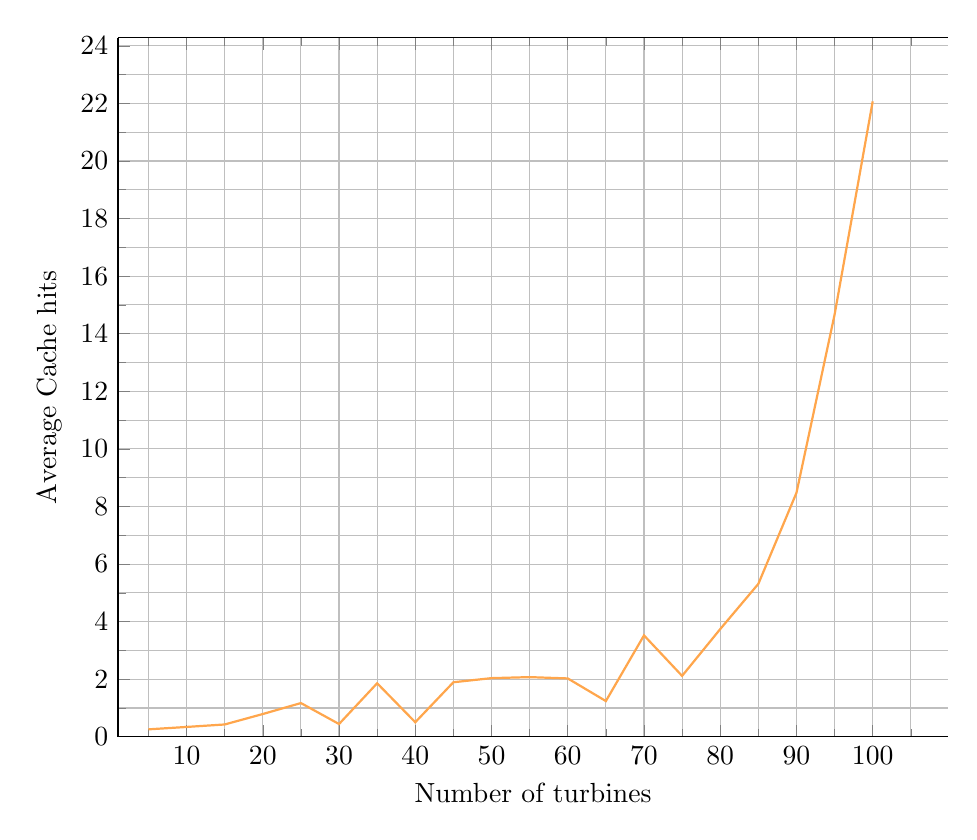
\begin{tikzpicture}
\begin{axis}
[
width=\resultsFigureWidthScale\textwidth,
axis y line*=left,
xlabel=Number of turbines,
ymin = 0,
xmin = 1,
ylabel=Average Cache hits,
%xtick={1, 2, 3, 4, 5, 6, 7, 8, 9, 10, 11, 12, 13, 14, 15, 16, 17, 18, 19, 20},
%xticklabels={5, 10, 15, 20, 25, 30, 35, 40, 45, 50, 55, 60, 65, 70, 75, 80, 85, 90, 95, 100},
%boxplot/draw direction=y,
grid=both,
minor tick num=1
]
%\buildBoxPlot[black]{0}{0}{0}{0}{0}
%\buildBoxPlot[black]{0}{0}{0}{0}{0}
%\buildBoxPlot[black]{0}{0}{0}{0}{0}
%\buildBoxPlot[black]{0}{0}{0}{0}{0}
%\buildBoxPlot[black]{0}{0}{0}{0}{0}
%\buildBoxPlot[black]{0}{0}{0}{0}{0}
%\buildBoxPlot[black]{0}{0}{0}{0}{0}
%\buildBoxPlot[black]{0}{0}{0}{0}{0}
%\buildBoxPlot[black]{0}{0}{0}{0}{0}
%\buildBoxPlot[black]{0}{0}{0}{0}{0}
%\buildBoxPlot[black]{0}{0}{0}{0}{0}
%\buildBoxPlot[black]{0}{0}{0}{0}{0}
%\buildBoxPlot[black]{0}{0}{0}{0}{0}
%\buildBoxPlot[black]{0}{0}{0}{0}{0}
%\buildBoxPlot[black]{0}{0}{0}{0}{0}
%\buildBoxPlot[black]{0}{0}{0}{0}{0}
%\buildBoxPlot[black]{0}{0}{0}{0}{0}
%\buildBoxPlot[black]{0}{0}{0}{0}{0}
%\buildBoxPlot[black]{0}{0}{0}{0}{0}
%\buildBoxPlot[black]{0}{0}{0}{0}{0}
\addplot[thick, orange!70] coordinates {
	(5 ,0.2591015249347438)
	(10 ,0.3423283799799435)
	(15 ,0.4286200856364344)
	(20 ,0.7913519050319182)
	(25 ,1.171919068056407)
	(30 ,0.4440826120490188)
	(35 ,1.8595523144717856)
	(40 ,0.506366007056297)
	(45 ,1.8951768000539848)
	(50 ,2.037951753081981)
	(55 ,2.0728170589196186)
	(60 ,2.0275369832294468)
	(65 ,1.2416290071090674)
	(70 ,3.5220372523313626)
	(75 ,2.115832267020478)
	(80 ,3.7417427229878832)
	(85 ,5.311682134712245)
	(90 ,8.473847137142263)
	(95 ,14.663734246038112)
	(100 ,22.06932793366117)
};
\end{axis}
\end{tikzpicture}
	\caption{Decentralized solution variable number of turbines experiment 1}
	\label{fig:exp:decen:turbines_cache}
\end{figure}


\cref{fig:exp:decen:turbines_cache} show the amount of cache reads the simulation had during part 2 of the experiment.
The plot almost lines up with a exponential curve. Also \cref{fig:exp:decen:turbines,fig:exp:decen:turbines_cache} seams to suddenly increase around 65 ms.

\subsection{Discussion}
\label{sec:disc:turbinesVScycletime}
In the current Siemens system the regulation cycle time of a single Park Pilot scales linearly with the number of turbines.
The aim of the decentralized solution is to detach the regulation cycle time from the number of turbines. 
Looking at \cref{fig:exp:decen:turbines} we see that the decentralized solution seems to be independent of the number of turbines, if the number of turbines is sufficiently low.
From 5 to 65 turbines the regulation cycle time is nearly constant at 20 ms.
The near constant regulation cycle time is caused by the fact that the regulation cycle in the decentralized solution is not forced to wait for data before running the regulation algorithm because data is continually shared between turbines. Adding a turbine to the decentralized solution adds an extra turbine state to factor into the setpoint calculation in the regulation algorithm. This and the added network traffic for the new turbine is the consequence of adding new turbines.

When looking at regulation cycle time of the decentralized solution we must also look at the number of cache reads.
As explained in \cref{sec:exp:performance} a cache read happens when a turbine does not provide a new turbine state package before the next regulation cycle is started.
This forces the regulation cycle to use old data read from cache.
Looking at \cref{fig:exp:decen:turbines_cache} we see that the average number of cache reads in the decentralized solution are below 2 and increasing slightly until we reach 65 turbines. From there the number of cache reads increase exponentially.

The increase in regulation cycle time and cache reads when the number of turbines reaches 65 can be explained by the fact that the network equipment of the test setup is approaching maximum throughput capacity which may cause lost or delayed network packages.
Since regulation cycle time in the decentralized system is dependent on the reception time of the oldest turbine state package as explained in \cref{sec:exp:performance} the loss or delay of network packages has a direct impact on regulation cycle time.
Similarly lost or delayed network packages increases the use of cached data. The increased regulation cycle time and cache reads are thus not a limitation of the decentralized solution but a limitation imposed by the test setup. In order to create a realistic comparison we must disregard the results that are a direct effect of the limitations of our test setup.

Disregarding the limitations imposed by the test setup we see that the regulation cycle time is constant. In terms of regulation cycle time the decentralized solution scales indefinitely. As stated above there is a small increase in regulation cycle time for every turbine added because the state of this turbine has to be taken into consideration when calculating new setpoints on all other turbines. This time addition is not visible on \cref{fig:exp:decen:turbines}. Thus the regulation cycle time will be affected by the addition of turbines but the effect is so small that it is indistinguishable by other factors. Looking at the raw test data 

Still disregarding the limitations imposed by the test setup when looking at the scale factor of the number of cache reads we see another result. The number of cache reads increases slowly with a factor of around 1 cache read for every 30 turbines added, which gives a scale factor of $1 / 30 = 0.033$.

The number of cache reads can be reduced by increasing the regulation cycle time as presented in \cref{fig:exp:decen:sleep-cache}.
Thus the factor deciding the time of the regulation cycle is the maximum number of average cache reads accepted for a single regulation cycle.

\section{\ref{PS:Q:Scalability}}

\textit{Will the regulation cycle time of the new decentralized solution scale better than the current Siemens system in terms of number of turbines per Park Pilot?}\newline\newline

\noindent As mentioned in \cref{cha:existingSystem} the centralized solution is a simulation of the current Siemens system. Thus to complete the comparison between the decentralized solution and the current Siemens system, the discussion section of this experiment also contains a discussion with regards to differences between the centralized solution and the current Siemens system (described in \cref{sec:CenAndCurrentSiemensSystemComparison}).

\subsection{Experiment}
\label{subsec:Exper:Scale}

The \ref{PS:Q:Scalability} problem asks for a comparison between the decentralized solution and the current Siemens system, in order to determine which of the systems scales best, in terms of decreasing the coupling between the regulation cycle time and the number of turbines. For this experiment we compare the results of the \ref{PS:Q:Performance} problem with acquired results from the centralized solution. Thus for this comparison, we study how the regulation cycle time changes when increasing the number of turbines for both systems.


\begin{figure}[b]
	%The figure show how regulation time differs central vs decantral
	\centering
	{\sffamily{Centralized approach}}
	\newline
	

{ %The brackets issolate the enviroment

\makeatletter
\ifcsname c@wavenum\endcsname %Only create one counter
\else
	\newcounter{wavenum}
\fi
\makeatother

\newcommand*{\bitvector}[3]{
  \draw[fill=#3] (t_cur) -- ++( .1, .3) -- ++(#2-.2,0) -- ++(.1, -.3)
                         -- ++(-.1,-.3) -- ++(.2-#2,0) -- cycle;
  \path (t_cur) -- node[anchor=mid] {#1} ++(#2,0) node[time] (t_cur) {};
}

% \known{val}{length}
\newcommand*{\known}[2]{
    \bitvector{#1}{#2}{white}
}

% \unknown{length}
\newcommand*{\unknown}[2]{
    \bitvector{#1}{#2}{black!20}
}

% \nextwave{name}
\newcommand{\nextwave}[1]{
  \path (0,\value{wavenum}) node[left] {#1} node[time] (t_cur) {};
  \addtocounter{wavenum}{-1}
}

% \begin{wave}[clkname]{num_waves}{clock_cycles}
\newenvironment{wave}{
  \begin{tikzpicture}[draw=black, yscale=.8,xscale=1]
    \tikzstyle{time}=[coordinate]
    \setlength{\unitlength}{1cm}
    \setcounter{wavenum}{0}
    
}{\end{tikzpicture}}

%%% End of timing.sty

\begin{wave}
 \nextwave{Regulation Time} \unknown{SendData}{2} \known{WaitForData}{5} \unknown{ReciveData}{2} \unknown{Calculate}{2}
\end{wave}
}

	\newline
	
	{\sffamily{Decentralized approach with seperate data reception}}
	

{ %The brackets issolate the enviroment

\makeatletter
\ifcsname c@wavenum\endcsname %Only create one counter
\else
	\newcounter{wavenum}
\fi
\makeatother

\newcommand*{\bitvector}[3]{
  \draw[fill=#3] (t_cur) -- ++( .1, .3) -- ++(#2-.2,0) -- ++(.1, -.3)
                         -- ++(-.1,-.3) -- ++(.2-#2,0) -- cycle;
  \path (t_cur) -- node[anchor=mid](textNode) {#1} ++(#2,0) node[time] (t_cur) {};
}

% \known{val}{length}
\newcommand*{\known}[2]{
    \bitvector{#1}{#2}{white}
}

% \unknown{length}
\newcommand*{\unknown}[2]{
    \bitvector{#1}{#2}{black!20}
}

% \nextwave{name}
\newcommand{\nextwave}[1]{
  %\path (0,\value{wavenum}) node[left] {#1} node[time] (t_cur) {};
  \path (0,\value{wavenum}) node[time] (t_cur) {};
  \addtocounter{wavenum}{-1}
}

%\newcommand{\timeSpanLabel}{
%	\node (CycleTimeLabel) [rectangle, above = 0.25cm of textNode, inner sep=10pt] {CycleTime};	  
%}

\newcommand{\timeSpanLabel}{
	\node (CycleTimeLabel) [rectangle, above = 1.02cm of t_cur, inner sep=0pt] {Regulation cycle time};
}

\newcommand{\timeSpanA}{
	\node (t_timeSpanA) [point, above = 0 of t_cur] {};	  
}

\newcommand{\timeSpanB}{
	\node (t_timeSpanB) [point, above =0 of t_cur] {};
	
	\graph[use existing nodes]{
		t_timeSpanA --[time span=1cm] CycleTimeLabel;
		CycleTimeLabel.south --[time span=-0.24cm] t_timeSpanB;
	}; 
	
}

%%% End of timing.sty

\begin{tikzpicture}[
	point/.style={inner sep=0pt}, %circle,minimum size=2pt,fill=red},
	draw=black, 
	yscale=.8,
	xscale=1,
	hv path/.style={to path={-| (\tikztotarget)}},
	vh path/.style={to path={|- (\tikztotarget)}},
	skip loop v/.style={to path={-- ++(#1,0) |- (\tikztotarget)}},		
	skip loop h/.style={to path={-- ++(0,#1) -| (\tikztotarget)}},
	time span/.style={to path={-- ++(0,#1) -| (\tikztotarget)}},
	graphs/every graph/.style={edges=rounded corners}	
]
	
\tikzstyle{time}=[coordinate]
\setlength{\unitlength}{1cm}
\setcounter{wavenum}{0}

	\nextwave{} \timeSpanA \unknown{readStates}{3} \unknown{calculate}{3} \timeSpanLabel \unknown{setSetpoint}{3} \unknown{sendState}{3} \timeSpanB \known{wait}{2}
	\nextwave{} \known{reciveStates}{14}
\end{tikzpicture}
}

	\caption{Centralized vs decentralized regulation time}
	\label{fig:timingCentralVSDecentral}
\end{figure}

The regulation cycle time of the decentralized solution is defined as the difference between the receive timestamp of the oldest turbine state (tOldestState) received and the timestamp sampled right after, a new turbine state has been sent (tSent):

$$regulation~cycle~time=tSent-tOldestState$$

The timestamp of the oldest turbine state is used to include network traffic in the regulation cycle time. Thus, if the decentralized solution is using cached data this will be reflected in the regulation cycle time, making the comparison between the centralized and decentralized solution more fair. 
%The aim is to compare the regulation cycle time including , therefore the turbine side centralized solution is not measured. This means that the decentralized version is at a slight disadvantage, since .

We use the following box plot type (for \cref{fig:exp:decen:sleep} and \cref{fig:exp:decen:turbines}): The central mark is the median, the edges of the box are the 25th and 75th percentiles, the whiskers extend to the most extreme data points not considered outliers, and outliers are plotted individually. The whisker length is denoted as 1.5 IQR. 

The following procedure is used each time the experiment is performed:

\begin{minipage}{\textwidth}
	\begin{enumerate}
		\item Start the system with N turbines.
		\item Make sure the system is stable.
		\item Start logging regulation cycle time.
		\item Stop logging after \experiemntRunTime.
		\end{enumerate}
\end{minipage}


\subsection{Results}

\begin{figure}[h!]
	\centering
%	\begin{tikzpicture}
\begin{axis}
[
	width=\resultsPlotWidthScale\textwidth,
	axis y line*=left,
	xlabel=Number of turbines,
	ylabel=Regulation cycle time (ms),
	ymin = 0,
	xmin = 1, xmax = 20,
	xtick={1, 2, 3, 4, 5, 6, 7, 8, 9, 10, 11, 12, 13, 14, 15, 16, 17, 18, 19},
	xticklabels={ , , 15, , 25, , 35, , 45, , 55, , 65, , 75, , 85, , 95},
%	xticklabels={5, 10, 15, 20, 25, 30, 35, 40, 45, 50, 55, 60, 65, 70, 75, 80, 85, 90, 95},
	boxplot/draw direction=y,
	ymajorgrids=true,
	yminorgrids=true,
%	minor y tick num=1,
	max space between ticks=17.5
]

%% /home/stefan/work/TestResults/Test4_Centralized_success_12-4-2014_2024/CentralizedLog2.csv
%\buildBoxPlot{0.871522}{0.955}{0.809034}{12.535623}{0.541744}
\buildBoxPlot[black]{0}{0}{0}{0}{0}

%% /home/stefan/work/TestResults/Test4_Centralized_success_12-4-2014_2024/CentralizedLog3.csv
\buildBoxPlot{1.168815}{1.310873}{1.081427}{24.566027}{0.591135}

%% /home/stefan/work/TestResults/Test4_Centralized_success_12-4-2014_2024/CentralizedLog4.csv
\buildBoxPlot{1.398871}{1.613768}{1.303639}{19.188073}{0.747894}

%% /home/stefan/work/TestResults/Test4_Centralized_success_12-4-2014_2024/CentralizedLog5.csv
\buildBoxPlot{1.722236}{1.981776}{1.596331}{13.257023}{1.077214}

%% /home/stefan/work/TestResults/Test4_Centralized_success_12-4-2014_2024/CentralizedLog6.csv
\buildBoxPlot{1.978881}{2.337657}{1.823133}{20.243534}{1.278172}

%% /home/stefan/work/TestResults/Test4_Centralized_success_12-4-2014_2024/CentralizedLog7.csv
\buildBoxPlot{2.985681}{3.527133}{2.724617}{102.89112}{1.917354}

%% /home/stefan/work/TestResults/Test4_Centralized_success_12-4-2014_2024/CentralizedLog8.csv
\buildBoxPlot{5.662268}{6.776311}{5.315074}{55.800126}{3.845115}

%% /home/stefan/work/TestResults/Test4_Centralized_success_12-4-2014_2024/CentralizedLog9.csv
\buildBoxPlot{14.607313}{22.842589}{10.21933}{40.119104}{7.578863}

%% /home/stefan/work/TestResults/Test4_Centralized_success_12-4-2014_2024/CentralizedLog10.csv
\buildBoxPlot{16.673738}{25.382756}{14.810635}{46.844742}{12.042462}

%% /home/stefan/work/TestResults/Test4_Centralized_success_12-4-2014_2024/CentralizedLog11.csv
\buildBoxPlot{20.220936}{27.962488}{19.190067}{63.348974}{17.058657}

%% /home/stefan/work/TestResults/Test4_Centralized_success_12-4-2014_2024/CentralizedLog12.csv
\buildBoxPlot{31.587407}{33.177592}{24.950794}{46.841843}{22.941051}

%% /home/stefan/work/TestResults/Test4_Centralized_success_12-4-2014_2024/CentralizedLog13.csv
\buildBoxPlot{36.93711}{38.790125}{32.230331}{51.398495}{29.702809}

%% /home/stefan/work/TestResults/Test4_Centralized_success_12-4-2014_2024/CentralizedLog14.csv
\buildBoxPlot{40.231022}{42.885333}{36.673407}{77.051599}{33.854906}

%% /home/stefan/work/TestResults/Test4_Centralized_success_12-4-2014_2024/CentralizedLog15.csv
\buildBoxPlot{45.380062}{48.694656}{42.841453}{225.894089}{39.402015}

%% /home/stefan/work/TestResults/Test4_Centralized_success_12-4-2014_2024/CentralizedLog16.csv
\buildBoxPlot{51.425649}{54.462315}{48.438981}{250.200229}{45.062697}

%% /home/stefan/work/TestResults/Test4_Centralized_success_12-4-2014_2024/CentralizedLog17.csv
\buildBoxPlot{58.196177}{62.557505}{55.582236}{271.626595}{51.598593}

%% /home/stefan/work/TestResults/Test4_Centralized_success_12-4-2014_2024/CentralizedLog18.csv
\buildBoxPlot{64.70376}{70.553035}{62.053219}{278.866888}{57.401402}

%% /home/stefan/work/TestResults/Test4_Centralized_success_12-4-2014_2024/CentralizedLog19.csv
\buildBoxPlot{73.715686}{80.566923}{69.809765}{287.542878}{65.698499}

%% /home/stefan/work/TestResults/Test4_Centralized_success_12-4-2014_2024/CentralizedLog20.csv
\buildBoxPlot{82.961949}{151.608592}{77.825807}{290.243704}{72.589561}


\addplot[thick, red!70] coordinates {
%	(1 ,0.871522)
	(2 ,1.168815)
	(3 ,1.398871)
	(4 ,1.722236)
	(5 ,1.978881)
	(6 ,2.985681)
	(7 ,5.662268)
	(8 ,14.607313)
	(9 ,16.673738)
	(10 ,20.220936)
	(11 ,31.587407)
	(12 ,36.93711)
	(13 ,40.231022)
	(14 ,45.380062)
	(15 ,51.425649)
	(16 ,58.196177)
	(17 ,64.70376)
	(18 ,73.715686)
	(19 ,82.961949)
};

\end{axis}
\end{tikzpicture}

%	% This file was created by matlab2tikz.
% Minimal pgfplots version: 1.3
%
%The latest updates can be retrieved from
%  http://www.mathworks.com/matlabcentral/fileexchange/22022-matlab2tikz
%where you can also make suggestions and rate matlab2tikz.
%
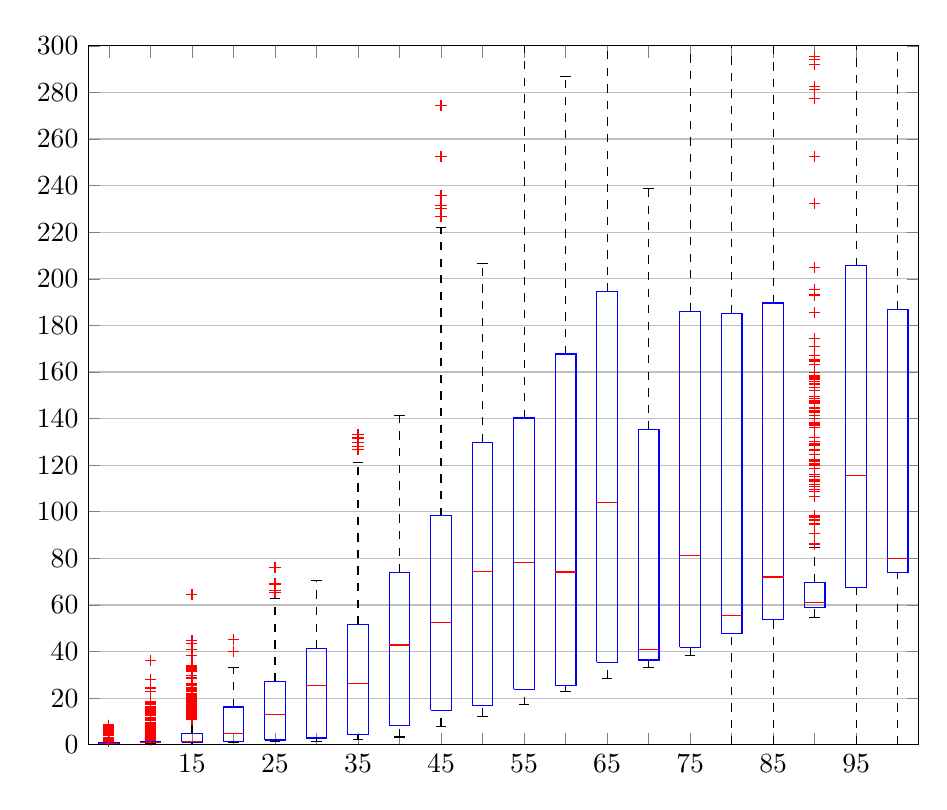
\begin{tikzpicture}

\begin{axis}[%
	width=\resultsPlotWidthScale\textwidth,
	xmin=0.5,
	xmax=20.5,
	xtick={1, 2, 3, 4, 5, 6, 7, 8, 9, 10, 11, 12, 13, 14, 15, 16, 17, 18, 19},
	xticklabels={ , , 15, , 25, , 35, , 45, , 55, , 65, , 75, , 85, , 95},
	ymin=0,
	ymax=300,
	ymajorgrids=true,
	yminorgrids=true,
	max space between ticks=17.5
]
\addplot [color=black,dashed,forget plot]
  table[row sep=crcr]{%
1	0.8717095\\
1	1.204627\\
};
\addplot [color=black,dashed,forget plot]
  table[row sep=crcr]{%
2	1.2604475\\
2	1.888937\\
};
\addplot [color=black,dashed,forget plot]
  table[row sep=crcr]{%
3	4.944662\\
3	10.675016\\
};
\addplot [color=black,dashed,forget plot]
  table[row sep=crcr]{%
4	16.2032205\\
4	33.311733\\
};
\addplot [color=black,dashed,forget plot]
  table[row sep=crcr]{%
5	27.053618\\
5	62.899558\\
};
\addplot [color=black,dashed,forget plot]
  table[row sep=crcr]{%
6	41.2910465\\
6	70.350287\\
};
\addplot [color=black,dashed,forget plot]
  table[row sep=crcr]{%
7	51.581584\\
7	121.085436\\
};
\addplot [color=black,dashed,forget plot]
  table[row sep=crcr]{%
8	73.910551\\
8	141.135822\\
};
\addplot [color=black,dashed,forget plot]
  table[row sep=crcr]{%
9	98.232932\\
9	222.18631\\
};
\addplot [color=black,dashed,forget plot]
  table[row sep=crcr]{%
10	129.9151\\
10	206.701738\\
};
\addplot [color=black,dashed,forget plot]
  table[row sep=crcr]{%
11	140.2385985\\
11	307.003647\\
};
\addplot [color=black,dashed,forget plot]
  table[row sep=crcr]{%
12	167.7148685\\
12	286.824347\\
};
\addplot [color=black,dashed,forget plot]
  table[row sep=crcr]{%
13	194.42233\\
13	426.984091\\
};
\addplot [color=black,dashed,forget plot]
  table[row sep=crcr]{%
14	135.221256\\
14	238.898358\\
};
\addplot [color=black,dashed,forget plot]
  table[row sep=crcr]{%
15	185.872368\\
15	399.208961\\
};
\addplot [color=black,dashed,forget plot]
  table[row sep=crcr]{%
16	185.049093\\
16	387.933056\\
};
\addplot [color=black,dashed,forget plot]
  table[row sep=crcr]{%
17	189.620724\\
17	390.403391\\
};
\addplot [color=black,dashed,forget plot]
  table[row sep=crcr]{%
18	69.756227\\
18	84.575222\\
};
\addplot [color=black,dashed,forget plot]
  table[row sep=crcr]{%
19	205.557893\\
19	412.155966\\
};
\addplot [color=black,dashed,forget plot]
  table[row sep=crcr]{%
20	186.7835205\\
20	355.119078\\
};
\addplot [color=black,dashed,forget plot]
  table[row sep=crcr]{%
1	0.452249\\
1	0.6489595\\
};
\addplot [color=black,dashed,forget plot]
  table[row sep=crcr]{%
2	0.604707\\
2	0.8393005\\
};
\addplot [color=black,dashed,forget plot]
  table[row sep=crcr]{%
3	0\\
3	1.1243275\\
};
\addplot [color=black,dashed,forget plot]
  table[row sep=crcr]{%
4	1.021879\\
4	1.5244415\\
};
\addplot [color=black,dashed,forget plot]
  table[row sep=crcr]{%
5	1.244611\\
5	2.061173\\
};
\addplot [color=black,dashed,forget plot]
  table[row sep=crcr]{%
6	1.524188\\
6	2.90871\\
};
\addplot [color=black,dashed,forget plot]
  table[row sep=crcr]{%
7	2.156496\\
7	4.2507545\\
};
\addplot [color=black,dashed,forget plot]
  table[row sep=crcr]{%
8	3.330849\\
8	8.282937\\
};
\addplot [color=black,dashed,forget plot]
  table[row sep=crcr]{%
9	7.831812\\
9	14.81487\\
};
\addplot [color=black,dashed,forget plot]
  table[row sep=crcr]{%
10	12.246399\\
10	16.6843555\\
};
\addplot [color=black,dashed,forget plot]
  table[row sep=crcr]{%
11	17.135656\\
11	23.771084\\
};
\addplot [color=black,dashed,forget plot]
  table[row sep=crcr]{%
12	22.778828\\
12	25.513819\\
};
\addplot [color=black,dashed,forget plot]
  table[row sep=crcr]{%
13	28.467515\\
13	35.4142585\\
};
\addplot [color=black,dashed,forget plot]
  table[row sep=crcr]{%
14	33.316406\\
14	36.380356\\
};
\addplot [color=black,dashed,forget plot]
  table[row sep=crcr]{%
15	38.153571\\
15	41.905524\\
};
\addplot [color=black,dashed,forget plot]
  table[row sep=crcr]{%
16	0\\
16	47.5835365\\
};
\addplot [color=black,dashed,forget plot]
  table[row sep=crcr]{%
17	0\\
17	53.6428275\\
};
\addplot [color=black,dashed,forget plot]
  table[row sep=crcr]{%
18	54.565993\\
18	58.849282\\
};
\addplot [color=black,dashed,forget plot]
  table[row sep=crcr]{%
19	0\\
19	67.47031\\
};
\addplot [color=black,dashed,forget plot]
  table[row sep=crcr]{%
20	0\\
20	74.0472365\\
};
\addplot [color=black,solid,forget plot]
  table[row sep=crcr]{%
0.875	1.204627\\
1.125	1.204627\\
};
\addplot [color=black,solid,forget plot]
  table[row sep=crcr]{%
1.875	1.888937\\
2.125	1.888937\\
};
\addplot [color=black,solid,forget plot]
  table[row sep=crcr]{%
2.875	10.675016\\
3.125	10.675016\\
};
\addplot [color=black,solid,forget plot]
  table[row sep=crcr]{%
3.875	33.311733\\
4.125	33.311733\\
};
\addplot [color=black,solid,forget plot]
  table[row sep=crcr]{%
4.875	62.899558\\
5.125	62.899558\\
};
\addplot [color=black,solid,forget plot]
  table[row sep=crcr]{%
5.875	70.350287\\
6.125	70.350287\\
};
\addplot [color=black,solid,forget plot]
  table[row sep=crcr]{%
6.875	121.085436\\
7.125	121.085436\\
};
\addplot [color=black,solid,forget plot]
  table[row sep=crcr]{%
7.875	141.135822\\
8.125	141.135822\\
};
\addplot [color=black,solid,forget plot]
  table[row sep=crcr]{%
8.875	222.18631\\
9.125	222.18631\\
};
\addplot [color=black,solid,forget plot]
  table[row sep=crcr]{%
9.875	206.701738\\
10.125	206.701738\\
};
\addplot [color=black,solid,forget plot]
  table[row sep=crcr]{%
10.875	307.003647\\
11.125	307.003647\\
};
\addplot [color=black,solid,forget plot]
  table[row sep=crcr]{%
11.875	286.824347\\
12.125	286.824347\\
};
\addplot [color=black,solid,forget plot]
  table[row sep=crcr]{%
12.875	426.984091\\
13.125	426.984091\\
};
\addplot [color=black,solid,forget plot]
  table[row sep=crcr]{%
13.875	238.898358\\
14.125	238.898358\\
};
\addplot [color=black,solid,forget plot]
  table[row sep=crcr]{%
14.875	399.208961\\
15.125	399.208961\\
};
\addplot [color=black,solid,forget plot]
  table[row sep=crcr]{%
15.875	387.933056\\
16.125	387.933056\\
};
\addplot [color=black,solid,forget plot]
  table[row sep=crcr]{%
16.875	390.403391\\
17.125	390.403391\\
};
\addplot [color=black,solid,forget plot]
  table[row sep=crcr]{%
17.875	84.575222\\
18.125	84.575222\\
};
\addplot [color=black,solid,forget plot]
  table[row sep=crcr]{%
18.875	412.155966\\
19.125	412.155966\\
};
\addplot [color=black,solid,forget plot]
  table[row sep=crcr]{%
19.875	355.119078\\
20.125	355.119078\\
};
\addplot [color=black,solid,forget plot]
  table[row sep=crcr]{%
0.875	0.452249\\
1.125	0.452249\\
};
\addplot [color=black,solid,forget plot]
  table[row sep=crcr]{%
1.875	0.604707\\
2.125	0.604707\\
};
\addplot [color=black,solid,forget plot]
  table[row sep=crcr]{%
2.875	0\\
3.125	0\\
};
\addplot [color=black,solid,forget plot]
  table[row sep=crcr]{%
3.875	1.021879\\
4.125	1.021879\\
};
\addplot [color=black,solid,forget plot]
  table[row sep=crcr]{%
4.875	1.244611\\
5.125	1.244611\\
};
\addplot [color=black,solid,forget plot]
  table[row sep=crcr]{%
5.875	1.524188\\
6.125	1.524188\\
};
\addplot [color=black,solid,forget plot]
  table[row sep=crcr]{%
6.875	2.156496\\
7.125	2.156496\\
};
\addplot [color=black,solid,forget plot]
  table[row sep=crcr]{%
7.875	3.330849\\
8.125	3.330849\\
};
\addplot [color=black,solid,forget plot]
  table[row sep=crcr]{%
8.875	7.831812\\
9.125	7.831812\\
};
\addplot [color=black,solid,forget plot]
  table[row sep=crcr]{%
9.875	12.246399\\
10.125	12.246399\\
};
\addplot [color=black,solid,forget plot]
  table[row sep=crcr]{%
10.875	17.135656\\
11.125	17.135656\\
};
\addplot [color=black,solid,forget plot]
  table[row sep=crcr]{%
11.875	22.778828\\
12.125	22.778828\\
};
\addplot [color=black,solid,forget plot]
  table[row sep=crcr]{%
12.875	28.467515\\
13.125	28.467515\\
};
\addplot [color=black,solid,forget plot]
  table[row sep=crcr]{%
13.875	33.316406\\
14.125	33.316406\\
};
\addplot [color=black,solid,forget plot]
  table[row sep=crcr]{%
14.875	38.153571\\
15.125	38.153571\\
};
\addplot [color=black,solid,forget plot]
  table[row sep=crcr]{%
15.875	0\\
16.125	0\\
};
\addplot [color=black,solid,forget plot]
  table[row sep=crcr]{%
16.875	0\\
17.125	0\\
};
\addplot [color=black,solid,forget plot]
  table[row sep=crcr]{%
17.875	54.565993\\
18.125	54.565993\\
};
\addplot [color=black,solid,forget plot]
  table[row sep=crcr]{%
18.875	0\\
19.125	0\\
};
\addplot [color=black,solid,forget plot]
  table[row sep=crcr]{%
19.875	0\\
20.125	0\\
};
\addplot [color=blue,solid,forget plot]
  table[row sep=crcr]{%
0.75	0.6489595\\
0.75	0.8717095\\
1.25	0.8717095\\
1.25	0.6489595\\
0.75	0.6489595\\
};
\addplot [color=blue,solid,forget plot]
  table[row sep=crcr]{%
1.75	0.8393005\\
1.75	1.2604475\\
2.25	1.2604475\\
2.25	0.8393005\\
1.75	0.8393005\\
};
\addplot [color=blue,solid,forget plot]
  table[row sep=crcr]{%
2.75	1.1243275\\
2.75	4.944662\\
3.25	4.944662\\
3.25	1.1243275\\
2.75	1.1243275\\
};
\addplot [color=blue,solid,forget plot]
  table[row sep=crcr]{%
3.75	1.5244415\\
3.75	16.2032205\\
4.25	16.2032205\\
4.25	1.5244415\\
3.75	1.5244415\\
};
\addplot [color=blue,solid,forget plot]
  table[row sep=crcr]{%
4.75	2.061173\\
4.75	27.053618\\
5.25	27.053618\\
5.25	2.061173\\
4.75	2.061173\\
};
\addplot [color=blue,solid,forget plot]
  table[row sep=crcr]{%
5.75	2.90871\\
5.75	41.2910465\\
6.25	41.2910465\\
6.25	2.90871\\
5.75	2.90871\\
};
\addplot [color=blue,solid,forget plot]
  table[row sep=crcr]{%
6.75	4.2507545\\
6.75	51.581584\\
7.25	51.581584\\
7.25	4.2507545\\
6.75	4.2507545\\
};
\addplot [color=blue,solid,forget plot]
  table[row sep=crcr]{%
7.75	8.282937\\
7.75	73.910551\\
8.25	73.910551\\
8.25	8.282937\\
7.75	8.282937\\
};
\addplot [color=blue,solid,forget plot]
  table[row sep=crcr]{%
8.75	14.81487\\
8.75	98.232932\\
9.25	98.232932\\
9.25	14.81487\\
8.75	14.81487\\
};
\addplot [color=blue,solid,forget plot]
  table[row sep=crcr]{%
9.75	16.6843555\\
9.75	129.9151\\
10.25	129.9151\\
10.25	16.6843555\\
9.75	16.6843555\\
};
\addplot [color=blue,solid,forget plot]
  table[row sep=crcr]{%
10.75	23.771084\\
10.75	140.2385985\\
11.25	140.2385985\\
11.25	23.771084\\
10.75	23.771084\\
};
\addplot [color=blue,solid,forget plot]
  table[row sep=crcr]{%
11.75	25.513819\\
11.75	167.7148685\\
12.25	167.7148685\\
12.25	25.513819\\
11.75	25.513819\\
};
\addplot [color=blue,solid,forget plot]
  table[row sep=crcr]{%
12.75	35.4142585\\
12.75	194.42233\\
13.25	194.42233\\
13.25	35.4142585\\
12.75	35.4142585\\
};
\addplot [color=blue,solid,forget plot]
  table[row sep=crcr]{%
13.75	36.380356\\
13.75	135.221256\\
14.25	135.221256\\
14.25	36.380356\\
13.75	36.380356\\
};
\addplot [color=blue,solid,forget plot]
  table[row sep=crcr]{%
14.75	41.905524\\
14.75	185.872368\\
15.25	185.872368\\
15.25	41.905524\\
14.75	41.905524\\
};
\addplot [color=blue,solid,forget plot]
  table[row sep=crcr]{%
15.75	47.5835365\\
15.75	185.049093\\
16.25	185.049093\\
16.25	47.5835365\\
15.75	47.5835365\\
};
\addplot [color=blue,solid,forget plot]
  table[row sep=crcr]{%
16.75	53.6428275\\
16.75	189.620724\\
17.25	189.620724\\
17.25	53.6428275\\
16.75	53.6428275\\
};
\addplot [color=blue,solid,forget plot]
  table[row sep=crcr]{%
17.75	58.849282\\
17.75	69.756227\\
18.25	69.756227\\
18.25	58.849282\\
17.75	58.849282\\
};
\addplot [color=blue,solid,forget plot]
  table[row sep=crcr]{%
18.75	67.47031\\
18.75	205.557893\\
19.25	205.557893\\
19.25	67.47031\\
18.75	67.47031\\
};
\addplot [color=blue,solid,forget plot]
  table[row sep=crcr]{%
19.75	74.0472365\\
19.75	186.7835205\\
20.25	186.7835205\\
20.25	74.0472365\\
19.75	74.0472365\\
};
\addplot [color=red,solid,forget plot]
  table[row sep=crcr]{%
0.75	0.727033\\
1.25	0.727033\\
};
\addplot [color=red,solid,forget plot]
  table[row sep=crcr]{%
1.75	0.9325085\\
2.25	0.9325085\\
};
\addplot [color=red,solid,forget plot]
  table[row sep=crcr]{%
2.75	1.3743515\\
3.25	1.3743515\\
};
\addplot [color=red,solid,forget plot]
  table[row sep=crcr]{%
3.75	4.791979\\
4.25	4.791979\\
};
\addplot [color=red,solid,forget plot]
  table[row sep=crcr]{%
4.75	13.090375\\
5.25	13.090375\\
};
\addplot [color=red,solid,forget plot]
  table[row sep=crcr]{%
5.75	25.5858225\\
6.25	25.5858225\\
};
\addplot [color=red,solid,forget plot]
  table[row sep=crcr]{%
6.75	26.3139895\\
7.25	26.3139895\\
};
\addplot [color=red,solid,forget plot]
  table[row sep=crcr]{%
7.75	42.7994295\\
8.25	42.7994295\\
};
\addplot [color=red,solid,forget plot]
  table[row sep=crcr]{%
8.75	52.370321\\
9.25	52.370321\\
};
\addplot [color=red,solid,forget plot]
  table[row sep=crcr]{%
9.75	74.509338\\
10.25	74.509338\\
};
\addplot [color=red,solid,forget plot]
  table[row sep=crcr]{%
10.75	78.4097345\\
11.25	78.4097345\\
};
\addplot [color=red,solid,forget plot]
  table[row sep=crcr]{%
11.75	74.1398775\\
12.25	74.1398775\\
};
\addplot [color=red,solid,forget plot]
  table[row sep=crcr]{%
12.75	103.919405\\
13.25	103.919405\\
};
\addplot [color=red,solid,forget plot]
  table[row sep=crcr]{%
13.75	40.8226565\\
14.25	40.8226565\\
};
\addplot [color=red,solid,forget plot]
  table[row sep=crcr]{%
14.75	81.151909\\
15.25	81.151909\\
};
\addplot [color=red,solid,forget plot]
  table[row sep=crcr]{%
15.75	55.4174655\\
16.25	55.4174655\\
};
\addplot [color=red,solid,forget plot]
  table[row sep=crcr]{%
16.75	71.9904755\\
17.25	71.9904755\\
};
\addplot [color=red,solid,forget plot]
  table[row sep=crcr]{%
17.75	60.9902745\\
18.25	60.9902745\\
};
\addplot [color=red,solid,forget plot]
  table[row sep=crcr]{%
18.75	115.484537\\
19.25	115.484537\\
};
\addplot [color=red,solid,forget plot]
  table[row sep=crcr]{%
19.75	79.967163\\
20.25	79.967163\\
};
\addplot [color=blue,only marks,mark=+,mark options={solid,draw=red},forget plot]
  table[row sep=crcr]{%
1	1.22142\\
1	1.223364\\
1	1.224134\\
1	1.233426\\
1	1.238923\\
1	1.249099\\
1	1.267809\\
1	1.284091\\
1	1.291981\\
1	1.319801\\
1	1.336661\\
1	1.415403\\
1	1.421902\\
1	1.503776\\
1	1.51294\\
1	1.532207\\
1	1.546875\\
1	1.547268\\
1	1.584143\\
1	1.589388\\
1	1.638589\\
1	1.811361\\
1	1.830223\\
1	1.831018\\
1	1.831122\\
1	1.835368\\
1	1.844371\\
1	2.105473\\
1	2.236183\\
1	2.251674\\
1	2.280143\\
1	2.299661\\
1	2.522178\\
1	2.750071\\
1	2.792578\\
1	3.25494\\
1	3.2941\\
1	3.929381\\
1	3.990809\\
1	4.137583\\
1	4.472371\\
1	4.537438\\
1	5.003565\\
1	5.006466\\
1	5.080215\\
1	5.089503\\
1	5.200881\\
1	5.250616\\
1	5.546884\\
1	5.625184\\
1	5.774674\\
1	5.797138\\
1	5.85168\\
1	5.899315\\
1	6.016238\\
1	6.033693\\
1	6.065686\\
1	6.074834\\
1	6.090889\\
1	6.127169\\
1	6.155085\\
1	6.426519\\
1	6.448381\\
1	6.519414\\
1	6.550741\\
1	6.582032\\
1	6.600282\\
1	6.737918\\
1	6.745443\\
1	6.750611\\
1	6.789309\\
1	6.798253\\
1	6.822493\\
1	6.995045\\
1	7.029346\\
1	7.053232\\
1	7.064158\\
1	7.07522\\
1	7.135983\\
1	7.160974\\
1	7.188216\\
1	7.222805\\
1	7.233565\\
1	7.249176\\
1	7.249689\\
1	7.27116\\
1	7.325184\\
1	7.352011\\
1	7.389161\\
1	7.426482\\
1	7.431757\\
1	7.463729\\
1	7.47152\\
1	7.522566\\
1	7.535727\\
1	7.545131\\
1	7.574998\\
1	7.635756\\
1	7.637039\\
1	7.681288\\
1	7.69941\\
1	7.713476\\
1	7.746304\\
1	7.80394\\
1	7.820249\\
1	7.866035\\
1	7.880942\\
1	7.974198\\
1	7.996921\\
1	8.016012\\
1	8.038029\\
1	8.038785\\
1	8.043832\\
1	8.054257\\
1	8.068841\\
1	8.094754\\
1	8.09828\\
1	8.100322\\
1	8.14914\\
1	8.165973\\
1	8.168417\\
1	8.197402\\
1	8.204572\\
1	8.211569\\
1	8.273737\\
1	8.292364\\
1	8.31482\\
1	8.323623\\
1	8.324661\\
1	8.35753\\
1	8.36441\\
1	8.443329\\
1	8.458258\\
};
\addplot [color=blue,only marks,mark=+,mark options={solid,draw=red},forget plot]
  table[row sep=crcr]{%
2	1.90167\\
2	1.911317\\
2	1.962956\\
2	1.968191\\
2	1.985629\\
2	1.990298\\
2	1.99821\\
2	1.999762\\
2	2.006972\\
2	2.01125\\
2	2.016703\\
2	2.060781\\
2	2.078726\\
2	2.084904\\
2	2.0886\\
2	2.149672\\
2	2.152386\\
2	2.157416\\
2	2.172206\\
2	2.210438\\
2	2.211897\\
2	2.265665\\
2	2.319203\\
2	2.320914\\
2	2.349612\\
2	2.398934\\
2	2.415953\\
2	2.462345\\
2	2.517542\\
2	2.518407\\
2	2.522352\\
2	2.559802\\
2	2.55986\\
2	2.588216\\
2	2.616982\\
2	2.640217\\
2	2.728957\\
2	2.763691\\
2	2.781829\\
2	2.796268\\
2	2.805757\\
2	2.809971\\
2	2.835864\\
2	2.857655\\
2	2.898538\\
2	2.902265\\
2	2.93052\\
2	2.958764\\
2	2.970508\\
2	2.981127\\
2	2.987679\\
2	2.993292\\
2	2.996044\\
2	3.003311\\
2	3.040946\\
2	3.044832\\
2	3.159759\\
2	3.171292\\
2	3.19803\\
2	3.223353\\
2	3.282729\\
2	3.322616\\
2	3.368547\\
2	3.522944\\
2	3.548358\\
2	3.57788\\
2	3.588871\\
2	3.709183\\
2	3.753555\\
2	4.156216\\
2	4.158493\\
2	4.17583\\
2	4.215829\\
2	4.22159\\
2	4.303591\\
2	4.378721\\
2	4.432432\\
2	4.496267\\
2	4.535655\\
2	4.562851\\
2	4.603645\\
2	4.626893\\
2	4.675847\\
2	4.697096\\
2	4.700302\\
2	4.704188\\
2	4.712042\\
2	4.793507\\
2	4.815152\\
2	4.857104\\
2	4.903281\\
2	4.925399\\
2	4.947763\\
2	5.141249\\
2	5.193353\\
2	5.338926\\
2	5.457376\\
2	5.767504\\
2	5.946886\\
2	6.065162\\
2	6.27828\\
2	6.380513\\
2	6.388238\\
2	6.414966\\
2	6.488282\\
2	6.659254\\
2	6.683566\\
2	6.877373\\
2	6.964909\\
2	7.118723\\
2	7.150523\\
2	7.184356\\
2	7.355692\\
2	7.373073\\
2	7.375065\\
2	7.387138\\
2	7.610728\\
2	7.827468\\
2	7.997416\\
2	8.003218\\
2	8.194986\\
2	8.875918\\
2	9.030813\\
2	9.168052\\
2	9.234478\\
2	9.240843\\
2	9.32023\\
2	9.355343\\
2	9.585629\\
2	9.632804\\
2	10.256122\\
2	10.54318\\
2	10.803498\\
2	10.849408\\
2	10.856044\\
2	10.946935\\
2	11.105923\\
2	11.112722\\
2	11.34085\\
2	11.612397\\
2	11.670481\\
2	11.712875\\
2	12.553934\\
2	12.558786\\
2	12.600901\\
2	12.730505\\
2	13.03436\\
2	13.59391\\
2	13.644562\\
2	14.067884\\
2	14.353523\\
2	14.417325\\
2	14.694076\\
2	14.763316\\
2	14.969792\\
2	14.992874\\
2	15.324704\\
2	15.355964\\
2	15.496052\\
2	15.989522\\
2	16.258874\\
2	16.543165\\
2	17.449576\\
2	17.943462\\
2	18.002392\\
2	18.307749\\
2	18.434977\\
2	22.673764\\
2	22.875711\\
2	24.368586\\
2	28.112777\\
2	36.326413\\
};
\addplot [color=blue,only marks,mark=+,mark options={solid,draw=red},forget plot]
  table[row sep=crcr]{%
3	10.712372\\
3	10.72463\\
3	10.824215\\
3	10.912497\\
3	10.934032\\
3	10.970966\\
3	11.133457\\
3	11.216931\\
3	11.239228\\
3	11.326209\\
3	11.337168\\
3	11.358172\\
3	11.440343\\
3	11.469403\\
3	11.51297\\
3	11.534249\\
3	11.610081\\
3	11.663412\\
3	11.694482\\
3	11.764268\\
3	11.788597\\
3	11.879232\\
3	11.88636\\
3	11.895998\\
3	11.951678\\
3	11.962575\\
3	12.136279\\
3	12.172993\\
3	12.18119\\
3	12.246693\\
3	12.301922\\
3	12.397148\\
3	12.649651\\
3	12.679065\\
3	12.736198\\
3	12.783409\\
3	12.846494\\
3	12.904049\\
3	12.983231\\
3	12.990299\\
3	12.999456\\
3	13.019261\\
3	13.133643\\
3	13.214978\\
3	13.294728\\
3	13.312276\\
3	13.361947\\
3	13.63175\\
3	13.636207\\
3	13.644932\\
3	13.834311\\
3	13.89846\\
3	13.935251\\
3	13.936967\\
3	13.984923\\
3	14.005203\\
3	14.066154\\
3	14.181378\\
3	14.216491\\
3	14.269401\\
3	14.371669\\
3	14.381037\\
3	14.391874\\
3	14.394386\\
3	14.406414\\
3	14.524739\\
3	14.653434\\
3	14.755178\\
3	14.874585\\
3	14.876075\\
3	15.017429\\
3	15.156781\\
3	15.305643\\
3	15.349046\\
3	15.516102\\
3	15.536637\\
3	15.593484\\
3	15.722859\\
3	16.133056\\
3	16.151682\\
3	16.251942\\
3	16.652387\\
3	16.82844\\
3	16.830175\\
3	16.845397\\
3	16.963685\\
3	17.027354\\
3	17.126082\\
3	17.175433\\
3	17.441423\\
3	17.447871\\
3	17.503013\\
3	18.054716\\
3	18.218939\\
3	18.232524\\
3	18.412774\\
3	18.471894\\
3	18.535344\\
3	18.547782\\
3	19.067263\\
3	19.288464\\
3	19.337552\\
3	19.550863\\
3	19.553737\\
3	19.65005\\
3	19.89144\\
3	20.004595\\
3	20.030844\\
3	20.076484\\
3	20.148205\\
3	20.24326\\
3	20.369406\\
3	20.548091\\
3	20.577104\\
3	20.989983\\
3	21.035488\\
3	21.265652\\
3	21.308726\\
3	21.391766\\
3	21.467402\\
3	21.487734\\
3	21.706475\\
3	21.806243\\
3	21.837835\\
3	21.847035\\
3	22.749871\\
3	23.003556\\
3	23.117597\\
3	23.162438\\
3	23.195855\\
3	23.466837\\
3	23.49557\\
3	23.627204\\
3	24.374648\\
3	24.422942\\
3	25.351046\\
3	25.782507\\
3	25.823924\\
3	25.873848\\
3	26.10141\\
3	26.481113\\
3	28.651801\\
3	28.687621\\
3	28.930998\\
3	29.6302\\
3	29.797236\\
3	31.334925\\
3	31.747665\\
3	32.48028\\
3	32.619401\\
3	33.017111\\
3	33.299365\\
3	33.710997\\
3	34.202288\\
3	38.391179\\
3	41.073174\\
3	43.384782\\
3	44.587852\\
3	44.822243\\
3	64.609355\\
};
\addplot [color=blue,only marks,mark=+,mark options={solid,draw=red},forget plot]
  table[row sep=crcr]{%
4	39.999706\\
4	45.044395\\
};
\addplot [color=blue,only marks,mark=+,mark options={solid,draw=red},forget plot]
  table[row sep=crcr]{%
5	65.437522\\
5	66.282007\\
5	68.917478\\
5	69.027589\\
5	69.32905\\
5	76.022717\\
};
\addplot [color=blue,only marks,mark=+,mark options={solid,draw=red},forget plot]
  table[row sep=crcr]{%
nan	nan\\
};
\addplot [color=blue,only marks,mark=+,mark options={solid,draw=red},forget plot]
  table[row sep=crcr]{%
7	126.57364\\
7	127.839887\\
7	129.633535\\
7	131.39321\\
7	131.744755\\
7	132.993896\\
};
\addplot [color=blue,only marks,mark=+,mark options={solid,draw=red},forget plot]
  table[row sep=crcr]{%
nan	nan\\
};
\addplot [color=blue,only marks,mark=+,mark options={solid,draw=red},forget plot]
  table[row sep=crcr]{%
9	226.846077\\
9	230.029879\\
9	231.330554\\
9	235.828114\\
9	252.531861\\
9	274.415257\\
};
\addplot [color=blue,only marks,mark=+,mark options={solid,draw=red},forget plot]
  table[row sep=crcr]{%
nan	nan\\
};
\addplot [color=blue,only marks,mark=+,mark options={solid,draw=red},forget plot]
  table[row sep=crcr]{%
11	328.644114\\
11	334.633811\\
11	347.48941\\
11	352.28358\\
};
\addplot [color=blue,only marks,mark=+,mark options={solid,draw=red},forget plot]
  table[row sep=crcr]{%
12	466.979415\\
12	790.974015\\
12	799.073064\\
12	807.138983\\
12	811.776466\\
12	825.995385\\
12	828.136598\\
12	828.636983\\
12	829.658051\\
12	830.027513\\
12	831.625153\\
12	860.149244\\
12	870.952407\\
12	925.896148\\
12	956.462884\\
12	980.212867\\
12	1475.832656\\
};
\addplot [color=blue,only marks,mark=+,mark options={solid,draw=red},forget plot]
  table[row sep=crcr]{%
13	436.452672\\
13	461.612621\\
13	464.72264\\
13	492.783547\\
};
\addplot [color=blue,only marks,mark=+,mark options={solid,draw=red},forget plot]
  table[row sep=crcr]{%
14	516.477803\\
14	521.131615\\
14	548.186438\\
14	553.249303\\
14	556.149607\\
14	574.576324\\
14	574.869284\\
14	577.742807\\
14	579.735296\\
14	584.686404\\
14	593.438547\\
14	596.380349\\
14	598.191485\\
14	598.84507\\
14	608.097375\\
14	617.101134\\
14	619.045276\\
14	619.953765\\
14	625.709395\\
14	629.279299\\
14	629.909969\\
14	637.550331\\
14	650.806984\\
14	655.873061\\
14	665.087489\\
14	668.713115\\
14	672.203926\\
14	674.734334\\
14	685.007391\\
14	685.276104\\
14	696.643168\\
14	702.755428\\
14	711.962523\\
14	713.90018\\
14	716.038134\\
14	717.987356\\
14	731.793634\\
14	732.812486\\
14	734.387525\\
14	735.553426\\
14	739.655719\\
14	741.138696\\
14	743.592059\\
14	749.511598\\
14	758.220628\\
14	767.173501\\
14	787.481231\\
14	791.741118\\
14	806.091296\\
14	807.148629\\
14	808.62873\\
14	813.961306\\
14	817.334614\\
14	817.433495\\
14	817.825926\\
14	820.848848\\
14	822.199013\\
14	827.34225\\
14	830.203037\\
14	830.9751\\
14	832.847263\\
14	834.140786\\
14	839.044581\\
14	845.966635\\
14	846.618104\\
14	854.936652\\
14	855.494969\\
14	859.374444\\
14	866.190171\\
14	870.842619\\
14	874.186476\\
14	883.121314\\
14	883.429961\\
14	885.89492\\
14	892.364938\\
14	895.886937\\
14	898.399519\\
14	900.917675\\
14	904.601228\\
14	919.104384\\
14	921.721725\\
14	923.317272\\
14	924.999961\\
14	929.178234\\
14	932.480675\\
14	938.552007\\
14	943.337044\\
14	947.603204\\
14	960.540944\\
14	961.402436\\
14	981.62104\\
14	981.970315\\
14	995.902458\\
14	998.546303\\
14	998.952993\\
14	1000.379985\\
14	1002.724105\\
14	1004.846879\\
14	1029.337594\\
14	1036.38101\\
14	1048.006164\\
14	1054.763013\\
14	1062.954368\\
14	1078.066665\\
14	1078.352514\\
14	1089.033734\\
14	1185.153126\\
14	1192.53254\\
};
\addplot [color=blue,only marks,mark=+,mark options={solid,draw=red},forget plot]
  table[row sep=crcr]{%
15	413.771069\\
15	415.537737\\
15	416.275727\\
15	416.638957\\
15	418.187265\\
15	429.650314\\
15	432.834924\\
15	436.729475\\
15	436.780207\\
15	447.391499\\
15	461.232542\\
15	468.187997\\
15	492.811488\\
};
\addplot [color=blue,only marks,mark=+,mark options={solid,draw=red},forget plot]
  table[row sep=crcr]{%
16	391.504739\\
16	393.266469\\
16	394.953183\\
16	400.079125\\
16	402.528077\\
16	402.59457\\
16	403.571968\\
16	404.604515\\
16	408.236184\\
16	410.786243\\
16	418.888676\\
16	421.719738\\
16	426.782423\\
16	429.928426\\
16	456.078929\\
16	456.144372\\
16	462.901035\\
16	466.222926\\
16	475.291873\\
16	494.781046\\
16	504.963081\\
16	512.937421\\
16	531.40812\\
16	537.32713\\
16	925.279886\\
};
\addplot [color=blue,only marks,mark=+,mark options={solid,draw=red},forget plot]
  table[row sep=crcr]{%
17	395.395536\\
17	396.185814\\
17	400.234754\\
17	400.919771\\
17	401.286572\\
17	401.44932\\
17	405.897657\\
17	406.550507\\
17	406.874901\\
17	409.850021\\
17	412.082702\\
17	412.29205\\
17	413.441619\\
17	418.860258\\
17	419.388793\\
17	420.870868\\
17	424.021534\\
17	425.802527\\
17	433.915915\\
17	434.473733\\
17	434.922242\\
17	435.478035\\
17	456.947733\\
17	460.611284\\
17	461.070377\\
17	467.248761\\
17	470.773971\\
17	474.641047\\
17	483.883285\\
17	488.567997\\
17	519.601736\\
17	529.774526\\
17	532.919833\\
17	541.579177\\
};
\addplot [color=blue,only marks,mark=+,mark options={solid,draw=red},forget plot]
  table[row sep=crcr]{%
18	86.159378\\
18	90.668505\\
18	94.440606\\
18	95.027982\\
18	96.177874\\
18	96.668815\\
18	97.51727\\
18	97.524343\\
18	97.961739\\
18	98.201713\\
18	106.504354\\
18	108.598272\\
18	109.386755\\
18	110.693345\\
18	111.61382\\
18	113.215588\\
18	113.998949\\
18	115.30506\\
18	116.084194\\
18	118.681951\\
18	119.784562\\
18	120.377811\\
18	120.539549\\
18	120.820783\\
18	121.687063\\
18	121.94637\\
18	122.404761\\
18	124.66292\\
18	126.255916\\
18	126.646287\\
18	128.615305\\
18	129.058219\\
18	129.308683\\
18	129.978064\\
18	130.146154\\
18	131.867658\\
18	136.250682\\
18	136.301259\\
18	136.915259\\
18	137.287311\\
18	137.924732\\
18	138.24477\\
18	138.363895\\
18	139.97497\\
18	141.274313\\
18	142.65381\\
18	142.785853\\
18	143.251243\\
18	144.273789\\
18	144.618031\\
18	144.701109\\
18	146.670355\\
18	147.314209\\
18	147.340368\\
18	147.720972\\
18	148.532556\\
18	149.467189\\
18	152.238227\\
18	153.168407\\
18	154.760433\\
18	154.964476\\
18	155.749014\\
18	155.98442\\
18	156.736876\\
18	156.750484\\
18	157.370718\\
18	157.404776\\
18	157.541901\\
18	157.872815\\
18	158.599972\\
18	159.809991\\
18	159.862686\\
18	163.176972\\
18	164.328241\\
18	165.034392\\
18	165.22673\\
18	167.233095\\
18	170.757205\\
18	174.316953\\
18	185.383809\\
18	192.887773\\
18	193.446229\\
18	195.274025\\
18	204.875554\\
18	232.269385\\
18	252.421417\\
18	277.39999\\
18	281.21265\\
18	282.571761\\
18	292.089637\\
18	294.003322\\
18	295.340114\\
18	306.445289\\
18	310.216001\\
18	316.22929\\
18	320.061372\\
18	330.890354\\
18	341.626899\\
18	343.59161\\
18	361.446167\\
18	363.177192\\
18	365.234394\\
18	366.878349\\
18	369.434197\\
18	370.667787\\
18	384.922705\\
18	385.597618\\
18	398.286229\\
18	401.356793\\
18	403.525193\\
18	414.925591\\
18	423.616652\\
18	430.152321\\
18	431.948109\\
18	432.166707\\
18	434.182315\\
18	435.375041\\
18	436.080741\\
18	437.833424\\
18	438.296088\\
18	447.623571\\
18	456.32524\\
18	463.234298\\
18	463.664204\\
18	466.356037\\
18	468.481474\\
18	476.083349\\
18	490.894297\\
18	495.430708\\
18	497.957675\\
18	510.218098\\
18	511.629683\\
18	518.204134\\
18	521.2447\\
18	524.646491\\
18	529.0453\\
18	548.305702\\
18	550.75314\\
18	556.834255\\
18	559.563867\\
18	560.999111\\
18	561.898571\\
18	563.805964\\
18	566.979079\\
18	569.477825\\
18	585.891429\\
18	593.081773\\
18	594.032478\\
18	598.754091\\
18	601.07898\\
18	603.136575\\
18	604.461436\\
18	606.685389\\
18	615.975934\\
18	620.809847\\
18	625.216047\\
18	630.588802\\
18	635.083585\\
18	642.385159\\
18	643.764533\\
18	644.34599\\
18	654.07332\\
18	655.095482\\
18	662.471484\\
18	672.075709\\
18	675.889961\\
18	678.529528\\
18	678.890173\\
18	679.892176\\
18	684.831434\\
18	693.301249\\
18	702.617589\\
18	704.800503\\
18	708.665208\\
18	708.977256\\
18	719.695982\\
18	735.567577\\
18	738.45188\\
18	749.744355\\
18	752.239752\\
18	753.363801\\
18	756.965076\\
18	774.785646\\
18	778.031152\\
18	780.012929\\
18	788.742864\\
18	800.74279\\
18	801.012185\\
18	801.979855\\
18	802.863591\\
18	804.011755\\
18	808.680876\\
18	811.645441\\
18	813.298084\\
18	814.704282\\
18	814.802509\\
18	827.255574\\
18	828.252459\\
18	830.491802\\
18	831.296368\\
18	844.512419\\
18	853.013952\\
18	855.333914\\
18	858.407994\\
18	862.556341\\
18	882.524993\\
18	888.049313\\
18	906.306451\\
18	927.21179\\
18	932.618025\\
18	958.612414\\
18	964.30056\\
18	988.822073\\
};
\addplot [color=blue,only marks,mark=+,mark options={solid,draw=red},forget plot]
  table[row sep=crcr]{%
19	413.669679\\
19	415.702375\\
19	421.262682\\
19	424.26178\\
19	426.089474\\
19	427.278767\\
19	428.492953\\
19	430.386802\\
19	432.204021\\
19	434.988013\\
19	441.578668\\
19	449.881596\\
19	452.992062\\
19	457.040734\\
19	466.596323\\
19	473.659686\\
19	474.630211\\
19	482.83727\\
19	489.9619\\
19	499.095103\\
19	505.514518\\
19	506.29266\\
19	511.546471\\
19	512.464355\\
19	522.876406\\
19	523.507248\\
19	570.948016\\
19	573.368585\\
19	617.511086\\
19	633.841826\\
19	1663.027196\\
};
\addplot [color=blue,only marks,mark=+,mark options={solid,draw=red},forget plot]
  table[row sep=crcr]{%
20	358.664953\\
20	360.072424\\
20	360.580857\\
20	361.947047\\
20	362.769512\\
20	362.804993\\
20	362.882224\\
20	366.635705\\
20	366.933437\\
20	369.319648\\
20	369.545844\\
20	370.231731\\
20	374.68687\\
20	375.767451\\
20	377.106097\\
20	377.145185\\
20	377.270073\\
20	377.810398\\
20	379.373097\\
20	381.619711\\
20	381.899586\\
20	383.899256\\
20	385.476556\\
20	388.002861\\
20	390.038386\\
20	391.134656\\
20	391.935506\\
20	393.59135\\
20	397.626386\\
20	398.893623\\
20	399.178755\\
20	399.205918\\
20	405.411734\\
20	405.963615\\
20	409.974305\\
20	412.016362\\
20	412.823962\\
20	413.978452\\
20	416.00232\\
20	416.415065\\
20	416.962054\\
20	417.219528\\
20	420.558141\\
20	421.591104\\
20	422.903165\\
20	426.921715\\
20	428.634563\\
20	429.690633\\
20	431.074876\\
20	437.859373\\
20	440.170792\\
20	440.193745\\
20	441.925947\\
20	445.547896\\
20	448.207225\\
20	450.135523\\
20	457.072721\\
20	462.446887\\
20	468.056455\\
20	469.564543\\
20	471.258957\\
20	471.842521\\
20	479.237943\\
20	484.914544\\
20	487.06593\\
20	490.47576\\
20	495.447743\\
20	496.395601\\
20	501.104952\\
20	503.873257\\
20	505.546379\\
20	509.227206\\
20	511.030046\\
20	514.989725\\
20	516.662709\\
20	517.272094\\
20	517.524197\\
20	519.17898\\
20	527.807278\\
20	530.516949\\
20	530.784088\\
20	538.294346\\
20	539.390593\\
20	545.104186\\
20	558.48975\\
20	561.960311\\
20	566.794466\\
20	574.553751\\
20	576.163225\\
20	582.59134\\
20	583.121629\\
20	597.917383\\
20	600.599936\\
20	607.524031\\
20	623.482585\\
20	627.745563\\
20	631.152009\\
20	633.042956\\
20	645.652143\\
20	667.712819\\
20	692.903214\\
20	698.927208\\
20	767.883767\\
20	784.149295\\
};
%\node[above, align=center, inner sep=0mm, text=black]
%at (axis cs:8.68,-12,0) {1};
%\node[above, align=center, inner sep=0mm, text=black]
%at (axis cs:26.04,-12,0) {2};
%\node[above, align=center, inner sep=0mm, text=black]
%at (axis cs:43.4,-12,0) {3};
%\node[above, align=center, inner sep=0mm, text=black]
%at (axis cs:60.76,-12,0) {4};
%\node[above, align=center, inner sep=0mm, text=black]
%at (axis cs:78.12,-12,0) {5};
%\node[above, align=center, inner sep=0mm, text=black]
%at (axis cs:95.48,-12,0) {6};
%\node[above, align=center, inner sep=0mm, text=black]
%at (axis cs:112.84,-12,0) {7};
%\node[above, align=center, inner sep=0mm, text=black]
%at (axis cs:130.2,-12,0) {8};
%\node[above, align=center, inner sep=0mm, text=black]
%at (axis cs:147.56,-12,0) {9};
%\node[above, align=center, inner sep=0mm, text=black]
%at (axis cs:164.92,-12,0) {10};
%\node[above, align=center, inner sep=0mm, text=black]
%at (axis cs:182.28,-12,0) {11};
%\node[above, align=center, inner sep=0mm, text=black]
%at (axis cs:199.64,-12,0) {12};
%\node[above, align=center, inner sep=0mm, text=black]
%at (axis cs:217,-12,0) {13};
%\node[above, align=center, inner sep=0mm, text=black]
%at (axis cs:234.36,-12,0) {14};
%\node[above, align=center, inner sep=0mm, text=black]
%at (axis cs:251.72,-12,0) {15};
%\node[above, align=center, inner sep=0mm, text=black]
%at (axis cs:269.08,-12,0) {16};
%\node[above, align=center, inner sep=0mm, text=black]
%at (axis cs:286.44,-12,0) {17};
%\node[above, align=center, inner sep=0mm, text=black]
%at (axis cs:303.8,-12,0) {18};
%\node[above, align=center, inner sep=0mm, text=black]
%at (axis cs:321.16,-12,0) {19};
%\node[above, align=center, inner sep=0mm, text=black]
%at (axis cs:338.52,-12,0) {20};
\end{axis}
\end{tikzpicture}%
	% This file was created by matlab2tikz.
% Minimal pgfplots version: 1.3
%
%The latest updates can be retrieved from
%  http://www.mathworks.com/matlabcentral/fileexchange/22022-matlab2tikz
%where you can also make suggestions and rate matlab2tikz.
%
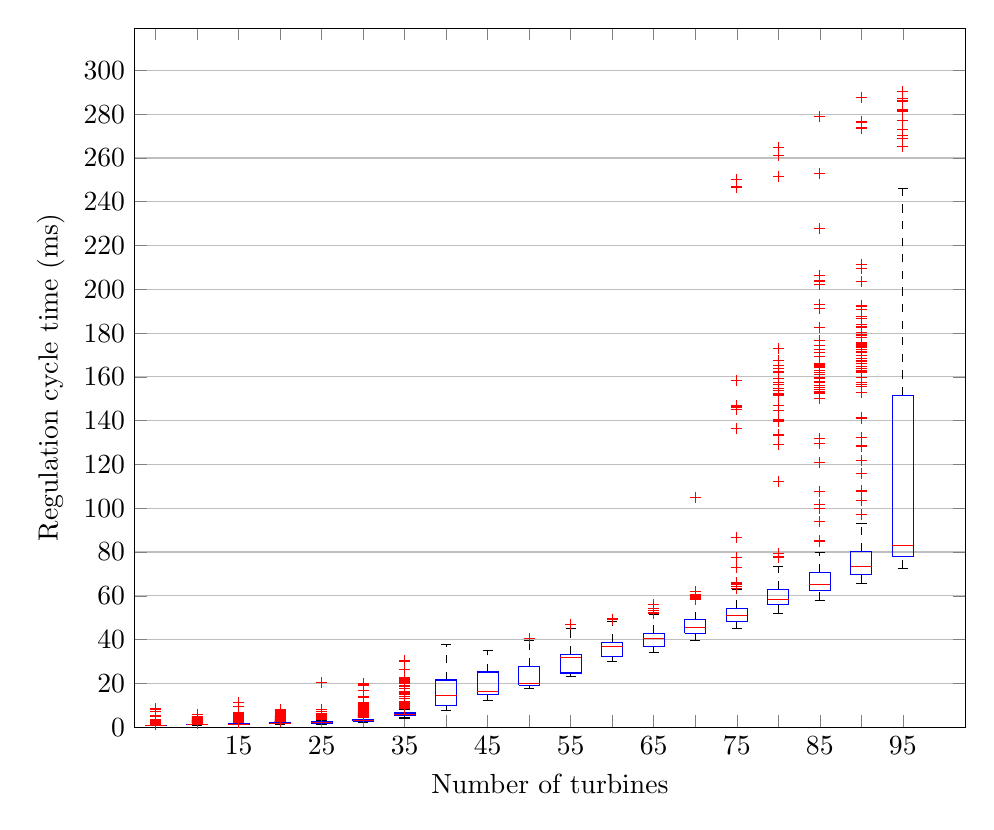
\begin{tikzpicture}

\begin{axis}[%
	width=\resultsPlotWidthScale\textwidth,
	xmin=0.5,
	xmax=20.5,
	xlabel=Number of turbines,
	ylabel=Regulation cycle time (ms),
	xtick={1, 2, 3, 4, 5, 6, 7, 8, 9, 10, 11, 12, 13, 14, 15, 16, 17, 18, 19},
	xticklabels={ , , 15, , 25, , 35, , 45, , 55, , 65, , 75, , 85, , 95},
	ymin=0,
%	ymax=300,
	ymajorgrids=true,
	yminorgrids=true,
	max space between ticks=17.5
]
\addplot [color=black,dashed,forget plot]
  table[row sep=crcr]{%
1	0.955499\\
1	1.156637\\
};
\addplot [color=black,dashed,forget plot]
  table[row sep=crcr]{%
2	1.370008\\
2	1.786582\\
};
\addplot [color=black,dashed,forget plot]
  table[row sep=crcr]{%
3	1.673373\\
3	2.174249\\
};
\addplot [color=black,dashed,forget plot]
  table[row sep=crcr]{%
4	1.958627\\
4	2.487973\\
};
\addplot [color=black,dashed,forget plot]
  table[row sep=crcr]{%
5	2.424964\\
5	3.23762\\
};
\addplot [color=black,dashed,forget plot]
  table[row sep=crcr]{%
6	3.359207\\
6	4.343135\\
};
\addplot [color=black,dashed,forget plot]
  table[row sep=crcr]{%
7	6.472311\\
7	8.243171\\
};
\addplot [color=black,dashed,forget plot]
  table[row sep=crcr]{%
8	21.564196\\
8	37.584364\\
};
\addplot [color=black,dashed,forget plot]
  table[row sep=crcr]{%
9	25.210282\\
9	34.938512\\
};
\addplot [color=black,dashed,forget plot]
  table[row sep=crcr]{%
10	27.678968\\
10	39.521324\\
};
\addplot [color=black,dashed,forget plot]
  table[row sep=crcr]{%
11	33.133063\\
11	45.066276\\
};
\addplot [color=black,dashed,forget plot]
  table[row sep=crcr]{%
12	38.659741\\
12	48.386618\\
};
\addplot [color=black,dashed,forget plot]
  table[row sep=crcr]{%
13	42.692349\\
13	51.64833\\
};
\addplot [color=black,dashed,forget plot]
  table[row sep=crcr]{%
14	48.995592\\
14	58.222076\\
};
\addplot [color=black,dashed,forget plot]
  table[row sep=crcr]{%
15	54.185768\\
15	62.996037\\
};
\addplot [color=black,dashed,forget plot]
  table[row sep=crcr]{%
16	62.88196\\
16	73.366361\\
};
\addplot [color=black,dashed,forget plot]
  table[row sep=crcr]{%
17	70.609667\\
17	79.750216\\
};
\addplot [color=black,dashed,forget plot]
  table[row sep=crcr]{%
18	80.203607\\
18	93.075175\\
};
\addplot [color=black,dashed,forget plot]
  table[row sep=crcr]{%
19	151.608592\\
19	246.076944\\
};
\addplot [color=black,dashed,forget plot]
  table[row sep=crcr]{%
1	0.691463\\
1	0.814662\\
};
\addplot [color=black,dashed,forget plot]
  table[row sep=crcr]{%
2	0.848749\\
2	1.088204\\
};
\addplot [color=black,dashed,forget plot]
  table[row sep=crcr]{%
3	1.082791\\
3	1.330567\\
};
\addplot [color=black,dashed,forget plot]
  table[row sep=crcr]{%
4	1.225531\\
4	1.59823\\
};
\addplot [color=black,dashed,forget plot]
  table[row sep=crcr]{%
5	1.440994\\
5	1.862917\\
};
\addplot [color=black,dashed,forget plot]
  table[row sep=crcr]{%
6	2.148756\\
6	2.694676\\
};
\addplot [color=black,dashed,forget plot]
  table[row sep=crcr]{%
7	4.178016\\
7	5.258074\\
};
\addplot [color=black,dashed,forget plot]
  table[row sep=crcr]{%
8	7.806459\\
8	9.763918\\
};
\addplot [color=black,dashed,forget plot]
  table[row sep=crcr]{%
9	12.116028\\
9	14.873879\\
};
\addplot [color=black,dashed,forget plot]
  table[row sep=crcr]{%
10	17.509834\\
10	19.152298\\
};
\addplot [color=black,dashed,forget plot]
  table[row sep=crcr]{%
11	23.186344\\
11	24.757905\\
};
\addplot [color=black,dashed,forget plot]
  table[row sep=crcr]{%
12	29.984252\\
12	32.129229\\
};
\addplot [color=black,dashed,forget plot]
  table[row sep=crcr]{%
13	33.953182\\
13	36.679471\\
};
\addplot [color=black,dashed,forget plot]
  table[row sep=crcr]{%
14	39.402015\\
14	42.832867\\
};
\addplot [color=black,dashed,forget plot]
  table[row sep=crcr]{%
15	45.162367\\
15	48.235799\\
};
\addplot [color=black,dashed,forget plot]
  table[row sep=crcr]{%
16	51.804628\\
16	55.840494\\
};
\addplot [color=black,dashed,forget plot]
  table[row sep=crcr]{%
17	57.925799\\
17	62.39761\\
};
\addplot [color=black,dashed,forget plot]
  table[row sep=crcr]{%
18	65.7218\\
18	69.72912\\
};
\addplot [color=black,dashed,forget plot]
  table[row sep=crcr]{%
19	72.589561\\
19	77.840082\\
};
\addplot [color=black,solid,forget plot]
  table[row sep=crcr]{%
0.875	1.156637\\
1.125	1.156637\\
};
\addplot [color=black,solid,forget plot]
  table[row sep=crcr]{%
1.875	1.786582\\
2.125	1.786582\\
};
\addplot [color=black,solid,forget plot]
  table[row sep=crcr]{%
2.875	2.174249\\
3.125	2.174249\\
};
\addplot [color=black,solid,forget plot]
  table[row sep=crcr]{%
3.875	2.487973\\
4.125	2.487973\\
};
\addplot [color=black,solid,forget plot]
  table[row sep=crcr]{%
4.875	3.23762\\
5.125	3.23762\\
};
\addplot [color=black,solid,forget plot]
  table[row sep=crcr]{%
5.875	4.343135\\
6.125	4.343135\\
};
\addplot [color=black,solid,forget plot]
  table[row sep=crcr]{%
6.875	8.243171\\
7.125	8.243171\\
};
\addplot [color=black,solid,forget plot]
  table[row sep=crcr]{%
7.875	37.584364\\
8.125	37.584364\\
};
\addplot [color=black,solid,forget plot]
  table[row sep=crcr]{%
8.875	34.938512\\
9.125	34.938512\\
};
\addplot [color=black,solid,forget plot]
  table[row sep=crcr]{%
9.875	39.521324\\
10.125	39.521324\\
};
\addplot [color=black,solid,forget plot]
  table[row sep=crcr]{%
10.875	45.066276\\
11.125	45.066276\\
};
\addplot [color=black,solid,forget plot]
  table[row sep=crcr]{%
11.875	48.386618\\
12.125	48.386618\\
};
\addplot [color=black,solid,forget plot]
  table[row sep=crcr]{%
12.875	51.64833\\
13.125	51.64833\\
};
\addplot [color=black,solid,forget plot]
  table[row sep=crcr]{%
13.875	58.222076\\
14.125	58.222076\\
};
\addplot [color=black,solid,forget plot]
  table[row sep=crcr]{%
14.875	62.996037\\
15.125	62.996037\\
};
\addplot [color=black,solid,forget plot]
  table[row sep=crcr]{%
15.875	73.366361\\
16.125	73.366361\\
};
\addplot [color=black,solid,forget plot]
  table[row sep=crcr]{%
16.875	79.750216\\
17.125	79.750216\\
};
\addplot [color=black,solid,forget plot]
  table[row sep=crcr]{%
17.875	93.075175\\
18.125	93.075175\\
};
\addplot [color=black,solid,forget plot]
  table[row sep=crcr]{%
18.875	246.076944\\
19.125	246.076944\\
};
\addplot [color=black,solid,forget plot]
  table[row sep=crcr]{%
0.875	0.691463\\
1.125	0.691463\\
};
\addplot [color=black,solid,forget plot]
  table[row sep=crcr]{%
1.875	0.848749\\
2.125	0.848749\\
};
\addplot [color=black,solid,forget plot]
  table[row sep=crcr]{%
2.875	1.082791\\
3.125	1.082791\\
};
\addplot [color=black,solid,forget plot]
  table[row sep=crcr]{%
3.875	1.225531\\
4.125	1.225531\\
};
\addplot [color=black,solid,forget plot]
  table[row sep=crcr]{%
4.875	1.440994\\
5.125	1.440994\\
};
\addplot [color=black,solid,forget plot]
  table[row sep=crcr]{%
5.875	2.148756\\
6.125	2.148756\\
};
\addplot [color=black,solid,forget plot]
  table[row sep=crcr]{%
6.875	4.178016\\
7.125	4.178016\\
};
\addplot [color=black,solid,forget plot]
  table[row sep=crcr]{%
7.875	7.806459\\
8.125	7.806459\\
};
\addplot [color=black,solid,forget plot]
  table[row sep=crcr]{%
8.875	12.116028\\
9.125	12.116028\\
};
\addplot [color=black,solid,forget plot]
  table[row sep=crcr]{%
9.875	17.509834\\
10.125	17.509834\\
};
\addplot [color=black,solid,forget plot]
  table[row sep=crcr]{%
10.875	23.186344\\
11.125	23.186344\\
};
\addplot [color=black,solid,forget plot]
  table[row sep=crcr]{%
11.875	29.984252\\
12.125	29.984252\\
};
\addplot [color=black,solid,forget plot]
  table[row sep=crcr]{%
12.875	33.953182\\
13.125	33.953182\\
};
\addplot [color=black,solid,forget plot]
  table[row sep=crcr]{%
13.875	39.402015\\
14.125	39.402015\\
};
\addplot [color=black,solid,forget plot]
  table[row sep=crcr]{%
14.875	45.162367\\
15.125	45.162367\\
};
\addplot [color=black,solid,forget plot]
  table[row sep=crcr]{%
15.875	51.804628\\
16.125	51.804628\\
};
\addplot [color=black,solid,forget plot]
  table[row sep=crcr]{%
16.875	57.925799\\
17.125	57.925799\\
};
\addplot [color=black,solid,forget plot]
  table[row sep=crcr]{%
17.875	65.7218\\
18.125	65.7218\\
};
\addplot [color=black,solid,forget plot]
  table[row sep=crcr]{%
18.875	72.589561\\
19.125	72.589561\\
};
\addplot [color=blue,solid,forget plot]
  table[row sep=crcr]{%
0.75	0.814662\\
0.75	0.955499\\
1.25	0.955499\\
1.25	0.814662\\
0.75	0.814662\\
};
\addplot [color=blue,solid,forget plot]
  table[row sep=crcr]{%
1.75	1.088204\\
1.75	1.370008\\
2.25	1.370008\\
2.25	1.088204\\
1.75	1.088204\\
};
\addplot [color=blue,solid,forget plot]
  table[row sep=crcr]{%
2.75	1.330567\\
2.75	1.673373\\
3.25	1.673373\\
3.25	1.330567\\
2.75	1.330567\\
};
\addplot [color=blue,solid,forget plot]
  table[row sep=crcr]{%
3.75	1.59823\\
3.75	1.958627\\
4.25	1.958627\\
4.25	1.59823\\
3.75	1.59823\\
};
\addplot [color=blue,solid,forget plot]
  table[row sep=crcr]{%
4.75	1.862917\\
4.75	2.424964\\
5.25	2.424964\\
5.25	1.862917\\
4.75	1.862917\\
};
\addplot [color=blue,solid,forget plot]
  table[row sep=crcr]{%
5.75	2.694676\\
5.75	3.359207\\
6.25	3.359207\\
6.25	2.694676\\
5.75	2.694676\\
};
\addplot [color=blue,solid,forget plot]
  table[row sep=crcr]{%
6.75	5.258074\\
6.75	6.472311\\
7.25	6.472311\\
7.25	5.258074\\
6.75	5.258074\\
};
\addplot [color=blue,solid,forget plot]
  table[row sep=crcr]{%
7.75	9.763918\\
7.75	21.564196\\
8.25	21.564196\\
8.25	9.763918\\
7.75	9.763918\\
};
\addplot [color=blue,solid,forget plot]
  table[row sep=crcr]{%
8.75	14.873879\\
8.75	25.210282\\
9.25	25.210282\\
9.25	14.873879\\
8.75	14.873879\\
};
\addplot [color=blue,solid,forget plot]
  table[row sep=crcr]{%
9.75	19.152298\\
9.75	27.678968\\
10.25	27.678968\\
10.25	19.152298\\
9.75	19.152298\\
};
\addplot [color=blue,solid,forget plot]
  table[row sep=crcr]{%
10.75	24.757905\\
10.75	33.133063\\
11.25	33.133063\\
11.25	24.757905\\
10.75	24.757905\\
};
\addplot [color=blue,solid,forget plot]
  table[row sep=crcr]{%
11.75	32.129229\\
11.75	38.659741\\
12.25	38.659741\\
12.25	32.129229\\
11.75	32.129229\\
};
\addplot [color=blue,solid,forget plot]
  table[row sep=crcr]{%
12.75	36.679471\\
12.75	42.692349\\
13.25	42.692349\\
13.25	36.679471\\
12.75	36.679471\\
};
\addplot [color=blue,solid,forget plot]
  table[row sep=crcr]{%
13.75	42.832867\\
13.75	48.995592\\
14.25	48.995592\\
14.25	42.832867\\
13.75	42.832867\\
};
\addplot [color=blue,solid,forget plot]
  table[row sep=crcr]{%
14.75	48.235799\\
14.75	54.185768\\
15.25	54.185768\\
15.25	48.235799\\
14.75	48.235799\\
};
\addplot [color=blue,solid,forget plot]
  table[row sep=crcr]{%
15.75	55.840494\\
15.75	62.88196\\
16.25	62.88196\\
16.25	55.840494\\
15.75	55.840494\\
};
\addplot [color=blue,solid,forget plot]
  table[row sep=crcr]{%
16.75	62.39761\\
16.75	70.609667\\
17.25	70.609667\\
17.25	62.39761\\
16.75	62.39761\\
};
\addplot [color=blue,solid,forget plot]
  table[row sep=crcr]{%
17.75	69.72912\\
17.75	80.203607\\
18.25	80.203607\\
18.25	69.72912\\
17.75	69.72912\\
};
\addplot [color=blue,solid,forget plot]
  table[row sep=crcr]{%
18.75	77.840082\\
18.75	151.608592\\
19.25	151.608592\\
19.25	77.840082\\
18.75	77.840082\\
};
\addplot [color=red,solid,forget plot]
  table[row sep=crcr]{%
0.75	0.874626\\
1.25	0.874626\\
};
\addplot [color=red,solid,forget plot]
  table[row sep=crcr]{%
1.75	1.1775345\\
2.25	1.1775345\\
};
\addplot [color=red,solid,forget plot]
  table[row sep=crcr]{%
2.75	1.4201575\\
3.25	1.4201575\\
};
\addplot [color=red,solid,forget plot]
  table[row sep=crcr]{%
3.75	1.716257\\
4.25	1.716257\\
};
\addplot [color=red,solid,forget plot]
  table[row sep=crcr]{%
4.75	1.9973935\\
5.25	1.9973935\\
};
\addplot [color=red,solid,forget plot]
  table[row sep=crcr]{%
5.75	2.903549\\
6.25	2.903549\\
};
\addplot [color=red,solid,forget plot]
  table[row sep=crcr]{%
6.75	5.5932275\\
7.25	5.5932275\\
};
\addplot [color=red,solid,forget plot]
  table[row sep=crcr]{%
7.75	14.5812775\\
8.25	14.5812775\\
};
\addplot [color=red,solid,forget plot]
  table[row sep=crcr]{%
8.75	16.4337625\\
9.25	16.4337625\\
};
\addplot [color=red,solid,forget plot]
  table[row sep=crcr]{%
9.75	20.091426\\
10.25	20.091426\\
};
\addplot [color=red,solid,forget plot]
  table[row sep=crcr]{%
10.75	31.692363\\
11.25	31.692363\\
};
\addplot [color=red,solid,forget plot]
  table[row sep=crcr]{%
11.75	36.8004425\\
12.25	36.8004425\\
};
\addplot [color=red,solid,forget plot]
  table[row sep=crcr]{%
12.75	40.4086135\\
13.25	40.4086135\\
};
\addplot [color=red,solid,forget plot]
  table[row sep=crcr]{%
13.75	45.333356\\
14.25	45.333356\\
};
\addplot [color=red,solid,forget plot]
  table[row sep=crcr]{%
14.75	50.8482875\\
15.25	50.8482875\\
};
\addplot [color=red,solid,forget plot]
  table[row sep=crcr]{%
15.75	58.49032\\
16.25	58.49032\\
};
\addplot [color=red,solid,forget plot]
  table[row sep=crcr]{%
16.75	65.293539\\
17.25	65.293539\\
};
\addplot [color=red,solid,forget plot]
  table[row sep=crcr]{%
17.75	73.479706\\
18.25	73.479706\\
};
\addplot [color=red,solid,forget plot]
  table[row sep=crcr]{%
18.75	82.948313\\
19.25	82.948313\\
};
\addplot [color=blue,only marks,mark=+,mark options={solid,draw=red},forget plot]
  table[row sep=crcr]{%
1	1.176103\\
1	1.178509\\
1	1.193344\\
1	1.20704\\
1	1.214954\\
1	1.221493\\
1	1.245021\\
1	1.316445\\
1	1.327208\\
1	1.524131\\
1	1.524274\\
1	1.543741\\
1	1.902597\\
1	2.169802\\
1	2.307744\\
1	2.476555\\
1	2.709384\\
1	2.981451\\
1	3.140805\\
1	3.283617\\
1	4.963499\\
1	5.363371\\
1	7.190786\\
1	8.30093\\
};
\addplot [color=blue,only marks,mark=+,mark options={solid,draw=red},forget plot]
  table[row sep=crcr]{%
2	1.793523\\
2	1.845619\\
2	1.848076\\
2	1.933673\\
2	1.99282\\
2	2.051408\\
2	2.120934\\
2	2.151493\\
2	2.249679\\
2	2.262758\\
2	2.300418\\
2	2.368791\\
2	2.401617\\
2	2.481835\\
2	2.53602\\
2	2.548682\\
2	2.576888\\
2	2.597632\\
2	2.677461\\
2	2.723364\\
2	2.740618\\
2	2.774466\\
2	2.867248\\
2	2.899936\\
2	2.944661\\
2	2.965056\\
2	2.96526\\
2	2.981629\\
2	3.089347\\
2	3.131373\\
2	3.180755\\
2	3.306036\\
2	3.332826\\
2	3.449926\\
2	3.489132\\
2	3.672439\\
2	3.706892\\
2	3.749078\\
2	3.877362\\
2	4.023028\\
2	4.389004\\
2	4.398121\\
2	4.401876\\
2	4.678904\\
2	4.779742\\
2	4.918733\\
2	5.075662\\
2	5.601809\\
};
\addplot [color=blue,only marks,mark=+,mark options={solid,draw=red},forget plot]
  table[row sep=crcr]{%
3	2.192261\\
3	2.222847\\
3	2.223433\\
3	2.239635\\
3	2.245748\\
3	2.337855\\
3	2.564155\\
3	2.566424\\
3	2.568352\\
3	2.629852\\
3	2.652528\\
3	2.703118\\
3	2.733534\\
3	2.764757\\
3	2.783863\\
3	2.828118\\
3	2.846928\\
3	2.984215\\
3	3.051839\\
3	3.071094\\
3	3.081963\\
3	3.230031\\
3	3.352067\\
3	3.690988\\
3	3.70011\\
3	3.71423\\
3	4.081016\\
3	4.251259\\
3	4.299668\\
3	4.317077\\
3	4.378226\\
3	4.655414\\
3	4.800068\\
3	5.335757\\
3	5.455589\\
3	5.596238\\
3	5.710081\\
3	5.790715\\
3	6.364993\\
3	6.679123\\
3	9.543143\\
3	11.395216\\
};
\addplot [color=blue,only marks,mark=+,mark options={solid,draw=red},forget plot]
  table[row sep=crcr]{%
4	2.503863\\
4	2.506996\\
4	2.518698\\
4	2.519083\\
4	2.524849\\
4	2.538949\\
4	2.539779\\
4	2.543708\\
4	2.590436\\
4	2.612976\\
4	2.624723\\
4	2.639969\\
4	2.692657\\
4	2.701875\\
4	2.702706\\
4	2.776353\\
4	2.834106\\
4	2.874534\\
4	2.903889\\
4	2.921809\\
4	2.947651\\
4	3.016038\\
4	3.18633\\
4	3.256435\\
4	3.289407\\
4	3.470499\\
4	3.523172\\
4	3.573076\\
4	3.614098\\
4	3.621255\\
4	3.757607\\
4	3.911986\\
4	4.033259\\
4	4.073237\\
4	4.338524\\
4	4.399647\\
4	4.630443\\
4	4.664954\\
4	4.779427\\
4	4.906645\\
4	4.925404\\
4	5.040655\\
4	5.079302\\
4	5.373808\\
4	6.030455\\
4	6.328306\\
4	6.626284\\
4	6.999776\\
4	7.221142\\
4	7.451491\\
4	7.916905\\
};
\addplot [color=blue,only marks,mark=+,mark options={solid,draw=red},forget plot]
  table[row sep=crcr]{%
5	3.320071\\
5	3.377586\\
5	3.423061\\
5	3.427332\\
5	3.53449\\
5	3.546939\\
5	3.746197\\
5	3.765826\\
5	3.782267\\
5	3.787644\\
5	3.824862\\
5	3.893861\\
5	3.959252\\
5	4.037436\\
5	4.097061\\
5	4.125631\\
5	4.133696\\
5	4.138075\\
5	4.147994\\
5	4.176374\\
5	4.421668\\
5	4.513637\\
5	4.616056\\
5	4.635814\\
5	4.753148\\
5	5.167944\\
5	5.19975\\
5	5.420932\\
5	5.455067\\
5	5.665121\\
5	5.721665\\
5	5.83401\\
5	5.87468\\
5	5.89412\\
5	5.921696\\
5	6.057049\\
5	6.131888\\
5	6.296973\\
5	6.321923\\
5	6.343328\\
5	7.090603\\
5	8.26168\\
5	20.243534\\
};
\addplot [color=blue,only marks,mark=+,mark options={solid,draw=red},forget plot]
  table[row sep=crcr]{%
6	4.495225\\
6	4.498673\\
6	4.498827\\
6	4.563186\\
6	4.587355\\
6	4.754654\\
6	5.009052\\
6	5.021732\\
6	5.102506\\
6	5.158721\\
6	5.167734\\
6	5.198709\\
6	5.23857\\
6	5.3746\\
6	5.400768\\
6	5.471458\\
6	5.487853\\
6	5.732529\\
6	5.758585\\
6	5.785591\\
6	5.904012\\
6	6.088597\\
6	6.13559\\
6	6.338497\\
6	6.607769\\
6	6.707598\\
6	6.847774\\
6	6.863557\\
6	6.923896\\
6	6.932131\\
6	6.966114\\
6	7.246241\\
6	7.552089\\
6	7.637072\\
6	8.035988\\
6	8.318994\\
6	8.349444\\
6	8.519427\\
6	8.777099\\
6	9.338181\\
6	9.720935\\
6	9.898789\\
6	10.188432\\
6	10.358991\\
6	10.590425\\
6	11.26527\\
6	13.649585\\
6	13.917339\\
6	16.898115\\
6	19.216894\\
6	19.71008\\
};
\addplot [color=blue,only marks,mark=+,mark options={solid,draw=red},forget plot]
  table[row sep=crcr]{%
7	8.35779\\
7	8.415277\\
7	8.473364\\
7	8.504532\\
7	8.506126\\
7	8.519745\\
7	8.553583\\
7	8.5815\\
7	8.663745\\
7	8.678187\\
7	8.683617\\
7	8.78386\\
7	8.849726\\
7	8.950628\\
7	8.987027\\
7	8.992308\\
7	9.120563\\
7	9.207595\\
7	9.23472\\
7	9.345101\\
7	9.398249\\
7	9.423573\\
7	9.439464\\
7	9.486276\\
7	9.521467\\
7	9.580156\\
7	9.590542\\
7	9.629696\\
7	9.657168\\
7	9.679038\\
7	9.768644\\
7	9.773259\\
7	9.820831\\
7	9.965677\\
7	10.269888\\
7	10.302693\\
7	10.323261\\
7	10.420508\\
7	10.88144\\
7	10.912448\\
7	10.912924\\
7	10.922096\\
7	11.006882\\
7	11.222083\\
7	11.30686\\
7	11.547859\\
7	13.009371\\
7	14.092999\\
7	14.86172\\
7	15.293268\\
7	15.773637\\
7	16.071576\\
7	17.524366\\
7	18.635734\\
7	18.86347\\
7	18.884021\\
7	19.925684\\
7	20.211662\\
7	20.368998\\
7	20.490724\\
7	20.838327\\
7	20.957185\\
7	21.053338\\
7	21.479073\\
7	21.720464\\
7	21.952807\\
7	22.450527\\
7	26.466628\\
7	29.810133\\
7	29.924012\\
7	30.656609\\
};
\addplot [color=blue,only marks,mark=+,mark options={solid,draw=red},forget plot]
  table[row sep=crcr]{%
nan	nan\\
};
\addplot [color=blue,only marks,mark=+,mark options={solid,draw=red},forget plot]
  table[row sep=crcr]{%
nan	nan\\
};
\addplot [color=blue,only marks,mark=+,mark options={solid,draw=red},forget plot]
  table[row sep=crcr]{%
10	40.572149\\
};
\addplot [color=blue,only marks,mark=+,mark options={solid,draw=red},forget plot]
  table[row sep=crcr]{%
11	46.841843\\
};
\addplot [color=blue,only marks,mark=+,mark options={solid,draw=red},forget plot]
  table[row sep=crcr]{%
12	49.32547\\
12	49.39728\\
};
\addplot [color=blue,only marks,mark=+,mark options={solid,draw=red},forget plot]
  table[row sep=crcr]{%
13	51.734931\\
13	52.263042\\
13	52.479868\\
13	53.346653\\
13	53.380803\\
13	54.235959\\
13	56.218855\\
};
\addplot [color=blue,only marks,mark=+,mark options={solid,draw=red},forget plot]
  table[row sep=crcr]{%
14	58.24263\\
14	58.359494\\
14	58.779699\\
14	59.255721\\
14	59.797221\\
14	59.956779\\
14	59.989437\\
14	60.023581\\
14	60.358906\\
14	60.684411\\
14	61.858036\\
14	104.953184\\
};
\addplot [color=blue,only marks,mark=+,mark options={solid,draw=red},forget plot]
  table[row sep=crcr]{%
15	63.495834\\
15	64.370846\\
15	65.078212\\
15	65.674834\\
15	65.803883\\
15	65.835327\\
15	66.021914\\
15	66.103339\\
15	73.001122\\
15	77.636315\\
15	86.826142\\
15	136.487634\\
15	145.283402\\
15	146.099428\\
15	146.233285\\
15	146.323243\\
15	146.921872\\
15	158.423312\\
15	246.362832\\
15	246.722952\\
15	250.200229\\
};
\addplot [color=blue,only marks,mark=+,mark options={solid,draw=red},forget plot]
  table[row sep=crcr]{%
16	77.720929\\
16	79.177628\\
16	112.408851\\
16	128.969515\\
16	133.462981\\
16	139.858548\\
16	140.725977\\
16	144.612062\\
16	146.817379\\
16	151.383076\\
16	151.881108\\
16	151.922485\\
16	152.242982\\
16	153.688064\\
16	154.509165\\
16	156.475983\\
16	157.507242\\
16	159.324566\\
16	162.256717\\
16	164.015403\\
16	165.32339\\
16	167.323423\\
16	172.786236\\
16	251.349021\\
16	261.289044\\
16	264.827819\\
};
\addplot [color=blue,only marks,mark=+,mark options={solid,draw=red},forget plot]
  table[row sep=crcr]{%
17	85.033259\\
17	85.168934\\
17	93.984073\\
17	99.985429\\
17	101.754141\\
17	107.502865\\
17	120.708505\\
17	129.533025\\
17	131.685524\\
17	150.07707\\
17	152.531279\\
17	152.848707\\
17	153.515564\\
17	154.184764\\
17	154.425517\\
17	155.223244\\
17	155.325952\\
17	156.040595\\
17	157.51096\\
17	157.745791\\
17	157.763823\\
17	157.78978\\
17	159.313071\\
17	159.792905\\
17	161.075164\\
17	161.182074\\
17	161.201118\\
17	162.147412\\
17	163.084965\\
17	164.144737\\
17	164.432633\\
17	164.531559\\
17	165.276971\\
17	165.915944\\
17	166.24057\\
17	169.122972\\
17	170.956902\\
17	172.574969\\
17	174.203491\\
17	174.230232\\
17	176.682499\\
17	182.438894\\
17	191.366639\\
17	192.967176\\
17	202.370675\\
17	203.807066\\
17	206.229644\\
17	227.845875\\
17	252.720361\\
17	278.866888\\
};
\addplot [color=blue,only marks,mark=+,mark options={solid,draw=red},forget plot]
  table[row sep=crcr]{%
18	97.320739\\
18	103.607594\\
18	107.896473\\
18	116.060945\\
18	121.809576\\
18	128.452211\\
18	132.177856\\
18	141.230189\\
18	152.923783\\
18	155.730984\\
18	156.691553\\
18	157.523825\\
18	159.835414\\
18	159.897403\\
18	161.962464\\
18	162.510937\\
18	162.565594\\
18	163.007536\\
18	163.988911\\
18	164.705291\\
18	165.959133\\
18	167.195639\\
18	167.26318\\
18	167.489415\\
18	167.573509\\
18	168.458682\\
18	169.70467\\
18	171.087881\\
18	171.523672\\
18	171.531448\\
18	171.659207\\
18	172.561978\\
18	172.716008\\
18	173.315331\\
18	173.869469\\
18	174.119127\\
18	174.807872\\
18	175.47089\\
18	178.054177\\
18	178.925643\\
18	179.325541\\
18	180.261783\\
18	182.703061\\
18	183.168246\\
18	183.804264\\
18	186.546645\\
18	187.398376\\
18	190.73619\\
18	192.117568\\
18	192.334748\\
18	192.687149\\
18	203.621105\\
18	209.714732\\
18	211.529157\\
18	273.591922\\
18	274.074762\\
18	276.443283\\
18	287.542878\\
};
\addplot [color=blue,only marks,mark=+,mark options={solid,draw=red},forget plot]
  table[row sep=crcr]{%
19	265.296814\\
19	268.749173\\
19	270.245766\\
19	273.069504\\
19	277.122711\\
19	281.054363\\
19	281.926684\\
19	282.148412\\
19	285.594887\\
19	286.16293\\
19	287.331069\\
19	290.243704\\
};
\node[above, align=center, inner sep=0mm, text=black]
at (axis cs:9.13684210526316,-12,0) {1};
\node[above, align=center, inner sep=0mm, text=black]
at (axis cs:27.4105263157895,-12,0) {2};
\node[above, align=center, inner sep=0mm, text=black]
at (axis cs:45.6842105263158,-12,0) {3};
\node[above, align=center, inner sep=0mm, text=black]
at (axis cs:63.9578947368421,-12,0) {4};
\node[above, align=center, inner sep=0mm, text=black]
at (axis cs:82.2315789473684,-12,0) {5};
\node[above, align=center, inner sep=0mm, text=black]
at (axis cs:100.505263157895,-12,0) {6};
\node[above, align=center, inner sep=0mm, text=black]
at (axis cs:118.778947368421,-12,0) {7};
\node[above, align=center, inner sep=0mm, text=black]
at (axis cs:137.052631578947,-12,0) {8};
\node[above, align=center, inner sep=0mm, text=black]
at (axis cs:155.326315789474,-12,0) {9};
\node[above, align=center, inner sep=0mm, text=black]
at (axis cs:173.6,-12,0) {10};
\node[above, align=center, inner sep=0mm, text=black]
at (axis cs:191.873684210526,-12,0) {11};
\node[above, align=center, inner sep=0mm, text=black]
at (axis cs:210.147368421053,-12,0) {12};
\node[above, align=center, inner sep=0mm, text=black]
at (axis cs:228.421052631579,-12,0) {13};
\node[above, align=center, inner sep=0mm, text=black]
at (axis cs:246.694736842105,-12,0) {14};
\node[above, align=center, inner sep=0mm, text=black]
at (axis cs:264.968421052632,-12,0) {15};
\node[above, align=center, inner sep=0mm, text=black]
at (axis cs:283.242105263158,-12,0) {16};
\node[above, align=center, inner sep=0mm, text=black]
at (axis cs:301.515789473684,-12,0) {17};
\node[above, align=center, inner sep=0mm, text=black]
at (axis cs:319.789473684211,-12,0) {18};
\node[above, align=center, inner sep=0mm, text=black]
at (axis cs:338.063157894737,-12,0) {19};
\end{axis}
\end{tikzpicture}%
	
	\caption{Centralized solution variable number of turbines}
	\label{fig:exp:cen:turbines}
\end{figure}

\Cref{fig:exp:cen:turbines} shows how the number of turbines influence the regulation cycle time of the centralized solution.
For every number of turbines 450 data points have been sampled. The reason for the limited amount of samples is that when running the experiment with 95 turbines the test setup is reaching it's limits. Data transfer speeds of up to 75 Mbit/s was observed. Since the maximum theoretical data transfer speed of the test setup is 100 Mbit/s it is reasonable to assume that a number of packages have been lost due to congestion. Thus, the experiment for 95 turbines only managed to log 450 data samples within the given experiment time. In order to create a boxplot with comparable values the sample set for each number of turbines was reduced to the 450 first points.
The limited amount of data samples account for the "holes" between outlier values. With more data samples these holes would be filled such that outliers are more evenly distributed from the top whisker to the most extreme outlier.

The median values from 5 to 30 turbines is increasing slightly. From 35 turbines and onward the median is linearly increasing.
From 75 turbines onward the outliers take on increasingly extreme values, which is when the test setup starts to be unable to handle the number of packages sent in the network. Results from 75 turbines and onward should be disregarded.

\subsection{Discussion}
The test results from the centralized solution presented in \cref{fig:exp:cen:turbines} shows how adding turbines increases the regulation cycle time. From 5 to 30 turbines the regulation time of the centralized solution increase slowly. After 35 turbines the increase in regulation cycle time becomes steeper. For every 15 turbines added the regulation cycle time increases with approximately $25 ms$. The relation between regulation cycle time and the number of turbines is caused by the direct impact the number of turbines have on the regulation cycle. The Park Pilot of the centralized solution must use additional time on querying each added turbine as well as wait for their individual reply before performing the regulation algorithm. Thus the scalability of the centralized solution is linear with a factor of approximately $25 / 15 = 1.667$ ms added regulation cycle time per added turbine.
The outliers of \cref{fig:exp:cen:turbines} is distributed fairly close around the medains from 5 to 70 turbines. From 75 turbines on the outliers quadruple in regulation cycle time which is a sign that the test setup has reached it's limits. The heavily increased regulation cycle time for the outliers is a result of lost or delayed network packages forcing the Park Pilot to wait for a retransmission of turbine state before the regulation cycle can be completed.

\subsubsection{Comparison of the decentralized solution and the centralized solution}
\label{sec:comp:decentralizedVScentralized}
The decentralized solution and the centralized solution is built with a very different architecture. This is reflected in the difference in the way the two solutions scale with the number of turbines.

\cref{fig:exp:cenVSDecen} shows the medians of \cref{fig:exp:decen:turbines,fig:exp:cen:turbines} where data that has been disregarded previously has been removed. Thus, the maximum number of turbines in \cref{fig:exp:cenVSDecen} is 70. 

\begin{figure}[h!]
	\centering
		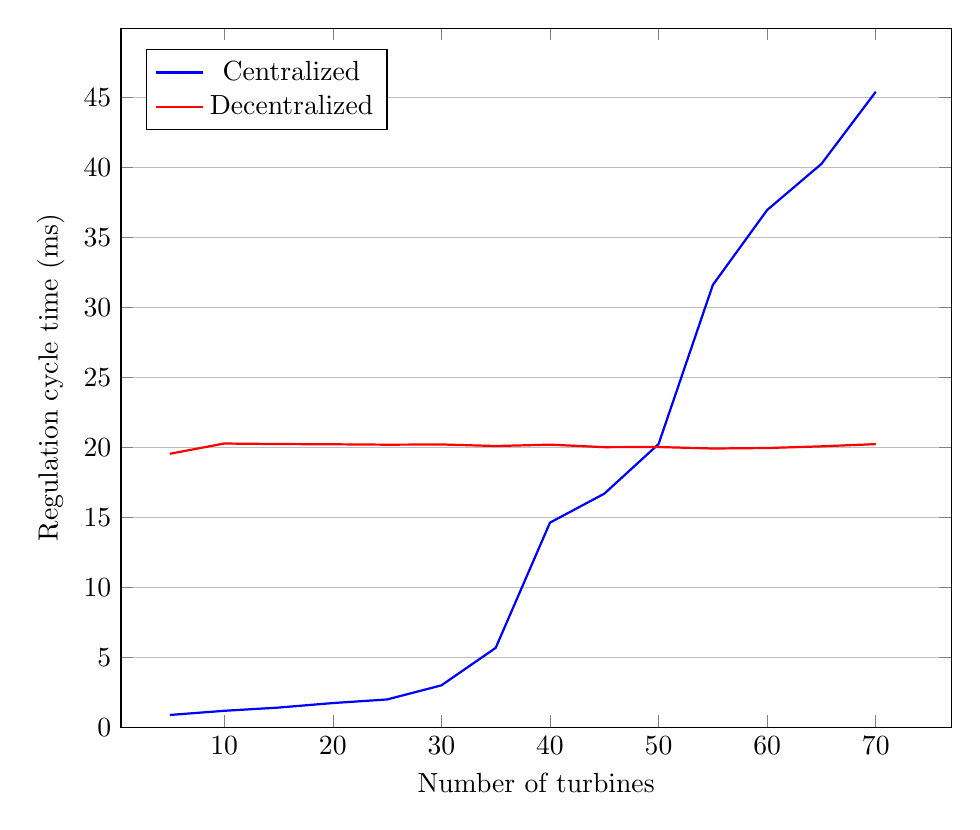
\begin{tikzpicture}
	
	\begin{axis}[%
	width=\resultsPlotWidthScale\textwidth,
	xmin=0.5,
%	xmax=20.5,
	xlabel=Number of turbines,
	ylabel=Regulation cycle time (ms),
%	xtick={1, 2, 3, 4, 5, 6, 7, 8, 9, 10, 11, 12, 13, 14, 15, 16, 17, 18, 19},
%	xticklabels={ 5, , 15, , 25, , 35, , 45, , 55, , 65, , 75, , 85, , 95},
	ymin=0,
	%	ymax=300,
	ymajorgrids=true,
%	yminorgrids=true,
%	max space between ticks=17.5,
	legend entries={Centralized,Decentralized},
	legend style={
		legend pos= north west,
	}
	]
	
	\addplot[thick, blue] coordinates {
		(5 ,0.871522)
		(10 ,1.168815)
		(15 ,1.398871)
		(20 ,1.722236)
		(25 ,1.978881)
		(30 ,2.985681)
		(35 ,5.662268)
		(40 ,14.607313)
		(45 ,16.673738)
		(50 ,20.220936)
		(55 ,31.587407)
		(60 ,36.93711)
		(65 ,40.231022)
		(70 ,45.380062)
%		(75 ,51.425649)
%		(80 ,58.196177)
%		(85 ,64.70376)
%		(90 ,73.715686)
%		(95 ,82.961949)
	};
	
	\addplot[thick, red] coordinates {
		(5 ,19.526002) 
		(10 ,20.257002)
		(15 ,20.221001)
		(20 ,20.203002)
		(25 ,20.174001)
		(30 ,20.190001)
		(35 ,20.079)
		(40 ,20.176)
		(45 ,19.998)
		(50 ,20.008)
		(55 ,19.902002)
		(60 ,19.937001)
		(65 ,20.056)
		(70 ,20.215)
%		(75 ,19.920001)
%		(80 ,20.129002)
%		(85 ,20.189001)
%		(90 ,20.902001)
%		(95 ,27.909001)
%		(100 ,43.314001)
	};
	\end{axis}
	\end{tikzpicture}	
	\caption{The centralized solution's median values compared with the decentralized solution's median values}
	\label{fig:exp:cenVSDecen}
\end{figure}

Looking at \cref{fig:exp:cenVSDecen} we see that the centralized and decentralized solutions scale very differently.
The decentralized solution scales constant with number of turbines from 5 to 70 turbines. The centralized solution scales linearly with the number of turbines from 5 to 30 turbines and from 30 to 70 turbines with a steeper slope. With the test setup used and a sleep time in the decentralized solution's regulation cycle at 20 ms the centralized solution scales better than the decentralized solution from 5 to 50 turbines. The decentralized solution scales better than the centralized solution from 50 to 70 turbines.
If the sleep time of the regulation cycle in the decentralized solution is lowered to for instance 10 ms the decentralized solution would scale better than the centralized solution from 38 turbines on. Lowering the sleep time of the regulation cycle in the decentralized solution will make the chance of cache reads increase as illustrated in \cref{fig:exp:decen:sleep-cache}.

One of the reasons for the constant scalability of the decentralized solution is the use of multicast in opposition to the centralized solution which uses unicast.
Using multicast the network communication is decreased compared to unicast, thus the network is less congested in the decentralized solution compared to the centralized solution.

Adding a turbine to the decentralized solution adds an extra turbine state to read into the setpoint calculation in the regulation algorithm, thus adding network traffic to the system.

As the test setup imposes limits on the number of turbines that can be simulated it is not possible to say anything concrete about how the scalability of the centralized and decentralized solution will be for any number of turbines higher than 70.
A qualified guess about the scalability can be provided though. The scalability of the centralized solution is expected to keep scaling linearly with the number of turbines. The decentralized solution will keep scaling with the number of turbines but as the number of turbines increase so will the number of cache reads. If the number of cache reads increases this will be reflected in the regulation cycle time. Thus, the scalability of the decentralized solution will not keep scaling at a constant level but the impact of increased cache reads remains to be further investigated.



\FloatBarrier

%The scalability of the centralized solution is linear with a factor of approximately $1.667$ ms added to regulation cycle time per turbine added to the system.
%The scalability of the decentralized solution, as described in \cref{sec:disc:turbinesVScycletime}, is small enough that it is indistinguishable from other factors in our test data and therefore we cannot calculate it. Thus the scalability of the decentralized solution is close to constant. This great improvement in scalability comes with a trade off in terms of cache reads. Adding additional turbines to the decentralized solution the number of cache reads increases with a factor of $0.033$ extra cache reads per added turbine which is still an improvement compared to the scale factor of the centralized solution. Arguably comparing the scalability of the number of cache reads in the decentralized solution with the scalability of the regulation cycle in the centralized solution is not a viable way to compare the scalability of the two solutions, but comparing the scalability of the regulation cycle of both solutions will not be a fair comparison either since the improvements in scalability of the decentralized solution comes at the price of increased numbers of cache reads.

\subsubsection{Comparison of the decentralized solution and the current Siemens system}
This section address the \ref{PS:Q:Scalability} problem of \cref{sec:problemStatement}.
Comparing the decentralized solution and the current Siemens system directly is impossible given the differences in environment and architecture. Introducing a centralized solution is an attempt to bridge this gap. By comparing the decentralized solution to the centralized solution and measuring the improvements/demotions we can transfer these measures to the current Siemens system and an imagined decentralized version of the current Siemens system.

Looking at \cref{sec:comp:decentralizedVScentralized} there is an advantage in scalability when running a decentralized solution compared to a centralized. This is underlined by the improvement in regulation cycle time of the decentralized solution compared to the centralized solution. The improvement of the scalability of the regulation cycle time comes at the price of the chance that the regulation may be performed on cached data.

Decentralizing the current Siemens system will enable improvements on other areas than regulation cycle time. By removing the centralized Park Pilots and the Wind Power Supervisor of the current Siemens solution the regulation of turbines, data storage and external communication of these must be decentralized and placed in the turbines themselves. This requires the use of software components that are able to handle regulation of turbines, data storage and external communication in a fashion such that if a turbine failure occurs other turbines can increase production to make up for the missing power production, provide access to the data collected on the failing turbine and handle external communication the failing turbine may have been handling. This increases the availability of the wind farm compared to the current Siemens system.





% include{Comparison}
\chapter{Conclusion}


\appendix
\addtocontents{toc}{\protect\setcounter{tocdepth}{0}}
\appendixpage

\chapter{Hardware Specifications}\label{appendix:HardwareSpecification}


\section{D-link DIR-855, Gigabyte Router}



\section{Macbook pro}\label{appendix:hardwareSpecification_pro}

\section{Asus UX32VD}\label{appendix:hardwareSpecification_asus}

\section{Macbook Air}\label{appendix:hardwareSpecification_air}
%
\chapter{Other results}\label{appendix:HardwareSpecification}
\subsection{Experiment \cref{PS:Q:Performance} Part 1}
\begin{figure}[h]
	\centering
	\begin{tikzpicture}
\begin{axis}
[
width=\textwidth,
axis y line*=left,
xlabel=Sleeptime (ms),
ylabel=Regulation cycle time (ms),
ymin = 0,
xtick={1, 2, 3, 4, 5, 6, 7, 8, 9},
xticklabels={10, 15, 20, 25, 30, 35, 40, 45, 50},
boxplot/draw direction=y
]

%% /home/stefan/work/TestResults/Test5_Decentralized_success_12-4-2014_2100/nSleepTime/DecentralizedLog0.csv
\buildBoxPlot{10.479001}{15.918002}{9.952001}{73.668}{0.351002}

%% /home/stefan/work/TestResults/Test5_Decentralized_success_12-4-2014_2100/nSleepTime/DecentralizedLog1.csv
\buildBoxPlot{15.092001}{15.350001}{14.615002}{35.264002}{1.741002}

%% /home/stefan/work/TestResults/Test5_Decentralized_success_12-4-2014_2100/nSleepTime/DecentralizedLog2.csv
\buildBoxPlot{19.940002}{20.344001}{19.065}{31.065001}{4.285}

%% /home/stefan/work/TestResults/Test5_Decentralized_success_12-4-2014_2100/nSleepTime/DecentralizedLog3.csv
\buildBoxPlot{25.049}{25.340002}{24.285001}{34.350001}{3.004001}

%% /home/stefan/work/TestResults/Test5_Decentralized_success_12-4-2014_2100/nSleepTime/DecentralizedLog4.csv
\buildBoxPlot{30.127001}{30.325}{29.743}{40.916}{18.242002}

%% /home/stefan/work/TestResults/Test5_Decentralized_success_12-4-2014_2100/nSleepTime/DecentralizedLog5.csv
\buildBoxPlot{35.128}{35.358001}{34.704}{47.280002}{1.504}

%% /home/stefan/work/TestResults/Test5_Decentralized_success_12-4-2014_2100/nSleepTime/DecentralizedLog6.csv
\buildBoxPlot{40.130002}{40.312001}{39.81}{51.402001}{25.482001}

%% /home/stefan/work/TestResults/Test5_Decentralized_success_12-4-2014_2100/nSleepTime/DecentralizedLog7.csv
\buildBoxPlot{45.186}{45.348001}{44.919}{59.214001}{15.009}

%% /home/stefan/work/TestResults/Test5_Decentralized_success_12-4-2014_2100/nSleepTime/DecentralizedLog8.csv
\buildBoxPlot{49.999001}{50.319002}{49.183002}{59.652}{4.503}


\addplot[thick, red!70] coordinates {
	(1 ,10.479001)
	(2 ,15.092001)
	(3 ,19.940002)
	(4 ,25.049)
	(5 ,30.127001)
	(6 ,35.128)
	(7 ,40.130002)
	(8 ,45.186)
	(9 ,49.999001)
	
};

\end{axis}
\end{tikzpicture}
	\caption{Decentralized solution with variable wait time cycle time extra experiment 1}
	\label{fig:exp:decen:sleep1}
\end{figure}

-
\begin{figure}[h]
	\centering
	\begin{tikzpicture}
\begin{axis}
[
width=\resultsFigureWidthScale\textwidth,
axis y line*=left,
xlabel=Sleeptime (ms),
ymin = 0,
ylabel=Average cache hits,
xtick={1, 2, 3, 4, 5, 6, 7, 8, 9},
xticklabels={10, 15, 20, 25, 30, 35, 40, 45, 50},
boxplot/draw direction=y
]
\buildBoxPlot[black]{0}{0}{0}{0}{0}
\buildBoxPlot[black]{0}{0}{0}{0}{0}
\buildBoxPlot[black]{0}{0}{0}{0}{0}
\buildBoxPlot[black]{0}{0}{0}{0}{0}
\buildBoxPlot[black]{0}{0}{0}{0}{0}
\buildBoxPlot[black]{0}{0}{0}{0}{0}
\buildBoxPlot[black]{0}{0}{0}{0}{0}
\buildBoxPlot[black]{0}{0}{0}{0}{0}
\buildBoxPlot[black]{0}{0}{0}{0}{0}
\addplot[thick, orange!70] coordinates {
	(1 ,6.085743962607115)
	(2 ,1.30948985528138)
	(3 ,1.938311112324131)
	(4 ,1.6288878136953286)
	(5 ,0.7463376395972676)
	(6 ,1.1345702327480605)
	(7 ,0.459182154121039)
	(8 ,0.6532183226081268)
	(9 ,1.2264147755115835)
};

%    \addplot [no markers, red] gnuplot [raw gnuplot] { % "raw gnuplot" allows us to use arbitrary gnuplot commands
%    	f(x) = a*exp(b*x); % Define the function to fit
%    	a=1; b=-0.001; % Set reasonable starting values here
%    	fit f(x) 'data.csv' u 1:4 via a,b; % Select the file, the columns (indexing starts at 1) and the variables
%    	plot [x=3000:4000] f(x); % Specify the range to plot
%    };


\end{axis}
\end{tikzpicture}
	\caption{Decentralized solution with variable wait time cache reads extra experiment 1}
	\label{fig:exp:decen:sleep1_cache}
\end{figure}

%\begin{figure}[h]
%	\centering
%	% This file was created by matlab2tikz.
% Minimal pgfplots version: 1.3
%
%The latest updates can be retrieved from
%  http://www.mathworks.com/matlabcentral/fileexchange/22022-matlab2tikz
%where you can also make suggestions and rate matlab2tikz.
%
\begin{tikzpicture}

\begin{axis}[%
width=\textwidth,
%height=3.636667in,
%at={(0.808889in,0.68in)},
%scale only axis,
%clip=false,
separate axis lines,
every outer x axis line/.append style={black},
every x tick label/.append style={font=\color{black}},
%xmin=0.5,
%xmax=9.5,
xtick={\empty},
every outer y axis line/.append style={black},
every y tick label/.append style={font=\color{black}},
%ymin=-7.0097979,
ymax=80,
ymajorgrids=true,
yminorgrids=true,
minor y tick num=1
]
\addplot [color=black,dashed,forget plot]
  table[row sep=crcr]{%
1	18.659501\\
1	31.534\\
};
\addplot [color=black,dashed,forget plot]
  table[row sep=crcr]{%
2	15.367\\
2	16.724\\
};
\addplot [color=black,dashed,forget plot]
  table[row sep=crcr]{%
3	20.371001\\
3	22.579002\\
};
\addplot [color=black,dashed,forget plot]
  table[row sep=crcr]{%
4	25.3150015\\
4	26.164002\\
};
\addplot [color=black,dashed,forget plot]
  table[row sep=crcr]{%
5	30.336001\\
5	31.231002\\
};
\addplot [color=black,dashed,forget plot]
  table[row sep=crcr]{%
6	35.326001\\
6	35.929001\\
};
\addplot [color=black,dashed,forget plot]
  table[row sep=crcr]{%
7	40.433001\\
7	41.601001\\
};
\addplot [color=black,dashed,forget plot]
  table[row sep=crcr]{%
8	45.328001\\
8	45.970001\\
};
\addplot [color=black,dashed,forget plot]
  table[row sep=crcr]{%
9	50.403002\\
9	52.495\\
};
\addplot [color=black,dashed,forget plot]
  table[row sep=crcr]{%
1	0.415002\\
1	10.0760015\\
};
\addplot [color=black,dashed,forget plot]
  table[row sep=crcr]{%
2	13.105\\
2	14.4620005\\
};
\addplot [color=black,dashed,forget plot]
  table[row sep=crcr]{%
3	16.692\\
3	18.899\\
};
\addplot [color=black,dashed,forget plot]
  table[row sep=crcr]{%
4	23.900001\\
4	24.749001\\
};
\addplot [color=black,dashed,forget plot]
  table[row sep=crcr]{%
5	28.844\\
5	29.739\\
};
\addplot [color=black,dashed,forget plot]
  table[row sep=crcr]{%
6	34.321001\\
6	34.924001\\
};
\addplot [color=black,dashed,forget plot]
  table[row sep=crcr]{%
7	38.486\\
7	39.6540015\\
};
\addplot [color=black,dashed,forget plot]
  table[row sep=crcr]{%
8	44.258\\
8	44.9\\
};
\addplot [color=black,dashed,forget plot]
  table[row sep=crcr]{%
9	46.916\\
9	49.008\\
};
\addplot [color=black,solid,forget plot]
  table[row sep=crcr]{%
0.875	31.534\\
1.125	31.534\\
};
\addplot [color=black,solid,forget plot]
  table[row sep=crcr]{%
1.875	16.724\\
2.125	16.724\\
};
\addplot [color=black,solid,forget plot]
  table[row sep=crcr]{%
2.875	22.579002\\
3.125	22.579002\\
};
\addplot [color=black,solid,forget plot]
  table[row sep=crcr]{%
3.875	26.164002\\
4.125	26.164002\\
};
\addplot [color=black,solid,forget plot]
  table[row sep=crcr]{%
4.875	31.231002\\
5.125	31.231002\\
};
\addplot [color=black,solid,forget plot]
  table[row sep=crcr]{%
5.875	35.929001\\
6.125	35.929001\\
};
\addplot [color=black,solid,forget plot]
  table[row sep=crcr]{%
6.875	41.601001\\
7.125	41.601001\\
};
\addplot [color=black,solid,forget plot]
  table[row sep=crcr]{%
7.875	45.970001\\
8.125	45.970001\\
};
\addplot [color=black,solid,forget plot]
  table[row sep=crcr]{%
8.875	52.495\\
9.125	52.495\\
};
\addplot [color=black,solid,forget plot]
  table[row sep=crcr]{%
0.875	0.415002\\
1.125	0.415002\\
};
\addplot [color=black,solid,forget plot]
  table[row sep=crcr]{%
1.875	13.105\\
2.125	13.105\\
};
\addplot [color=black,solid,forget plot]
  table[row sep=crcr]{%
2.875	16.692\\
3.125	16.692\\
};
\addplot [color=black,solid,forget plot]
  table[row sep=crcr]{%
3.875	23.900001\\
4.125	23.900001\\
};
\addplot [color=black,solid,forget plot]
  table[row sep=crcr]{%
4.875	28.844\\
5.125	28.844\\
};
\addplot [color=black,solid,forget plot]
  table[row sep=crcr]{%
5.875	34.321001\\
6.125	34.321001\\
};
\addplot [color=black,solid,forget plot]
  table[row sep=crcr]{%
6.875	38.486\\
7.125	38.486\\
};
\addplot [color=black,solid,forget plot]
  table[row sep=crcr]{%
7.875	44.258\\
8.125	44.258\\
};
\addplot [color=black,solid,forget plot]
  table[row sep=crcr]{%
8.875	46.916\\
9.125	46.916\\
};
\addplot [color=blue,solid,forget plot]
  table[row sep=crcr]{%
0.75	10.0760015\\
0.75	18.659501\\
1.25	18.659501\\
1.25	10.0760015\\
0.75	10.0760015\\
};
\addplot [color=blue,solid,forget plot]
  table[row sep=crcr]{%
1.75	14.4620005\\
1.75	15.367\\
2.25	15.367\\
2.25	14.4620005\\
1.75	14.4620005\\
};
\addplot [color=blue,solid,forget plot]
  table[row sep=crcr]{%
2.75	18.899\\
2.75	20.371001\\
3.25	20.371001\\
3.25	18.899\\
2.75	18.899\\
};
\addplot [color=blue,solid,forget plot]
  table[row sep=crcr]{%
3.75	24.749001\\
3.75	25.3150015\\
4.25	25.3150015\\
4.25	24.749001\\
3.75	24.749001\\
};
\addplot [color=blue,solid,forget plot]
  table[row sep=crcr]{%
4.75	29.739\\
4.75	30.336001\\
5.25	30.336001\\
5.25	29.739\\
4.75	29.739\\
};
\addplot [color=blue,solid,forget plot]
  table[row sep=crcr]{%
5.75	34.924001\\
5.75	35.326001\\
6.25	35.326001\\
6.25	34.924001\\
5.75	34.924001\\
};
\addplot [color=blue,solid,forget plot]
  table[row sep=crcr]{%
6.75	39.6540015\\
6.75	40.433001\\
7.25	40.433001\\
7.25	39.6540015\\
6.75	39.6540015\\
};
\addplot [color=blue,solid,forget plot]
  table[row sep=crcr]{%
7.75	44.9\\
7.75	45.328001\\
8.25	45.328001\\
8.25	44.9\\
7.75	44.9\\
};
\addplot [color=blue,solid,forget plot]
  table[row sep=crcr]{%
8.75	49.008\\
8.75	50.403002\\
9.25	50.403002\\
9.25	49.008\\
8.75	49.008\\
};
\addplot [color=red,solid,forget plot]
  table[row sep=crcr]{%
0.75	11.7570005\\
1.25	11.7570005\\
};
\addplot [color=red,solid,forget plot]
  table[row sep=crcr]{%
1.75	15.052\\
2.25	15.052\\
};
\addplot [color=red,solid,forget plot]
  table[row sep=crcr]{%
2.75	19.867\\
3.25	19.867\\
};
\addplot [color=red,solid,forget plot]
  table[row sep=crcr]{%
3.75	25.110001\\
4.25	25.110001\\
};
\addplot [color=red,solid,forget plot]
  table[row sep=crcr]{%
4.75	30.128\\
5.25	30.128\\
};
\addplot [color=red,solid,forget plot]
  table[row sep=crcr]{%
5.75	35.173001\\
6.25	35.173001\\
};
\addplot [color=red,solid,forget plot]
  table[row sep=crcr]{%
6.75	40.161001\\
7.25	40.161001\\
};
\addplot [color=red,solid,forget plot]
  table[row sep=crcr]{%
7.75	45.172002\\
8.25	45.172002\\
};
\addplot [color=red,solid,forget plot]
  table[row sep=crcr]{%
8.75	49.986001\\
9.25	49.986001\\
};

\addplot [color=blue,only marks,mark=+,mark options={solid,draw=red},forget plot]
  table[row sep=crcr]{%
1 31.537\\
1 31.545002\\
1 31.549001\\
1 31.556\\
1 31.557\\
1 31.557001\\
1 31.559002\\
1 31.562\\
1 31.564001\\
1 31.569\\
1 31.572001\\
1 31.572001\\
1 31.585002\\
1 31.586001\\
1 31.593\\
1 31.594\\
1 31.595001\\
1 31.607001\\
1 31.609001\\
1 31.615\\
1 31.616002\\
1 31.619\\
1 31.619001\\
1 31.621001\\
1 31.627\\
1 31.633\\
1 31.647\\
1 31.651001\\
1 31.655\\
1 31.660001\\
1 31.663001\\
1 31.663002\\
1 31.667001\\
1 31.669001\\
1 31.670001\\
1 31.675\\
1 31.678002\\
1 31.679001\\
1 31.680001\\
1 31.684002\\
1 31.687\\
1 31.689001\\
1 31.690001\\
1 31.690002\\
1 31.694\\
1 31.700002\\
1 31.701001\\
1 31.705\\
1 31.706\\
1 31.707\\
1 31.710001\\
1 31.719\\
1 31.719002\\
1 31.720001\\
1 31.730001\\
1 31.740001\\
1 31.749002\\
1 31.76\\
1 31.778002\\
1 31.779\\
1 31.785002\\
1 31.786001\\
1 31.787001\\
1 31.789001\\
1 31.792001\\
1 31.794001\\
1 31.799001\\
1 31.804002\\
1 31.813002\\
1 31.815\\
1 31.820002\\
1 31.821001\\
1 31.827002\\
1 31.829002\\
1 31.835001\\
1 31.836001\\
1 31.84\\
1 31.846\\
1 31.854001\\
1 31.855\\
1 31.858001\\
1 31.861002\\
1 31.863\\
1 31.869002\\
1 31.879001\\
1 31.882\\
1 31.883\\
1 31.893001\\
1 31.897001\\
1 31.902001\\
1 31.908001\\
1 31.911002\\
1 31.913001\\
1 31.924\\
1 31.924002\\
1 31.934\\
1 31.934\\
1 31.944\\
1 31.953001\\
1 31.958\\
1 31.958\\
1 31.967002\\
1 31.969\\
1 31.982001\\
1 31.987\\
1 31.989001\\
1 32.004\\
1 32.010002\\
1 32.014\\
1 32.014\\
1 32.021001\\
1 32.022001\\
1 32.024001\\
1 32.026\\
1 32.028\\
1 32.03\\
1 32.030001\\
1 32.031002\\
1 32.031002\\
1 32.033001\\
1 32.034001\\
1 32.038\\
1 32.038002\\
1 32.039001\\
1 32.043001\\
1 32.043001\\
1 32.044001\\
1 32.045001\\
1 32.048\\
1 32.048\\
1 32.052001\\
1 32.060001\\
1 32.060001\\
1 32.060002\\
1 32.066001\\
1 32.066002\\
1 32.070001\\
1 32.070001\\
1 32.077\\
1 32.092001\\
1 32.092001\\
1 32.093\\
1 32.098\\
1 32.102\\
1 32.107\\
1 32.107002\\
1 32.110002\\
1 32.113\\
1 32.113\\
1 32.117\\
1 32.118001\\
1 32.119001\\
1 32.127001\\
1 32.127002\\
1 32.145\\
1 32.145001\\
1 32.157\\
1 32.166002\\
1 32.167002\\
1 32.177001\\
1 32.185\\
1 32.188001\\
1 32.188002\\
1 32.189\\
1 32.192\\
1 32.193001\\
1 32.200002\\
1 32.202\\
1 32.204\\
1 32.21\\
1 32.211002\\
1 32.218001\\
1 32.218001\\
1 32.230001\\
1 32.234002\\
1 32.238002\\
1 32.240001\\
1 32.244\\
1 32.245001\\
1 32.250001\\
1 32.252001\\
1 32.258001\\
1 32.268001\\
1 32.268001\\
1 32.27\\
1 32.274002\\
1 32.278\\
1 32.283\\
1 32.284\\
1 32.287\\
1 32.288002\\
1 32.288002\\
1 32.289001\\
1 32.291001\\
1 32.292001\\
1 32.292001\\
1 32.302001\\
1 32.308001\\
1 32.309002\\
1 32.313001\\
1 32.315\\
1 32.317001\\
1 32.323001\\
1 32.324\\
1 32.325001\\
1 32.327001\\
1 32.333001\\
1 32.337001\\
1 32.349\\
1 32.350001\\
1 32.357\\
1 32.359001\\
1 32.361001\\
1 32.361001\\
1 32.362\\
1 32.366001\\
1 32.366002\\
1 32.371001\\
1 32.371001\\
1 32.378\\
1 32.381002\\
1 32.386001\\
1 32.388\\
1 32.391\\
1 32.391001\\
1 32.392001\\
1 32.404001\\
1 32.405001\\
1 32.406\\
1 32.412001\\
1 32.413001\\
1 32.416\\
1 32.418001\\
1 32.424\\
1 32.428002\\
1 32.431\\
1 32.437002\\
1 32.441001\\
1 32.443001\\
1 32.444002\\
1 32.446001\\
1 32.447\\
1 32.455001\\
1 32.459001\\
1 32.459002\\
1 32.463002\\
1 32.469\\
1 32.469001\\
1 32.472001\\
1 32.473\\
1 32.475\\
1 32.491001\\
1 32.491001\\
1 32.494001\\
1 32.495001\\
1 32.498002\\
1 32.511\\
1 32.511001\\
1 32.514\\
1 32.514002\\
1 32.519001\\
1 32.523001\\
1 32.524001\\
1 32.533001\\
1 32.534002\\
1 32.535002\\
1 32.536\\
1 32.537\\
1 32.539002\\
1 32.546\\
1 32.547002\\
1 32.549001\\
1 32.551001\\
1 32.552\\
1 32.556001\\
1 32.559001\\
1 32.562001\\
1 32.568\\
1 32.576001\\
1 32.576001\\
1 32.577001\\
1 32.582001\\
1 32.585\\
1 32.586001\\
1 32.589\\
1 32.59\\
1 32.594001\\
1 32.596001\\
1 32.597\\
1 32.603001\\
1 32.61\\
1 32.610002\\
1 32.615001\\
1 32.626001\\
1 32.627\\
1 32.631001\\
1 32.634001\\
1 32.642\\
1 32.662\\
1 32.669001\\
1 32.676001\\
1 32.684\\
1 32.686002\\
1 32.687001\\
1 32.689\\
1 32.691\\
1 32.695\\
1 32.696002\\
1 32.698\\
1 32.705\\
1 32.710001\\
1 32.712001\\
1 32.718001\\
1 32.722001\\
1 32.755001\\
1 32.763\\
1 32.766001\\
1 32.767001\\
1 32.767001\\
1 32.777001\\
1 32.78\\
1 32.784001\\
1 32.785002\\
1 32.788001\\
1 32.789001\\
1 32.790001\\
1 32.791\\
1 32.793\\
1 32.795\\
1 32.796\\
1 32.8\\
1 32.803\\
1 32.814002\\
1 32.816001\\
1 32.823002\\
1 32.838\\
1 32.838\\
1 32.840002\\
1 32.841002\\
1 32.850002\\
1 32.852\\
1 32.857002\\
1 32.857002\\
1 32.861\\
1 32.861001\\
1 32.863001\\
1 32.875001\\
1 32.877001\\
1 32.888\\
1 32.914001\\
1 32.920001\\
1 32.946\\
1 32.947\\
1 32.948001\\
1 32.952\\
1 32.957002\\
1 32.959002\\
1 32.961\\
1 32.965\\
1 32.966\\
1 32.968001\\
1 32.985001\\
1 32.988001\\
1 32.989001\\
1 32.991\\
1 32.993\\
1 32.994001\\
1 32.998\\
1 33.001001\\
1 33.015001\\
1 33.016001\\
1 33.016002\\
1 33.018001\\
1 33.019\\
1 33.021002\\
1 33.022\\
1 33.033\\
1 33.036\\
1 33.036001\\
1 33.042002\\
1 33.049\\
1 33.049001\\
1 33.057001\\
1 33.059\\
1 33.060001\\
1 33.063001\\
1 33.065001\\
1 33.068\\
1 33.075\\
1 33.076\\
1 33.078001\\
1 33.079002\\
1 33.08\\
1 33.089\\
1 33.100001\\
1 33.102\\
1 33.107001\\
1 33.111\\
1 33.115001\\
1 33.123\\
1 33.124\\
1 33.148001\\
1 33.154\\
1 33.154002\\
1 33.155\\
1 33.157\\
1 33.162\\
1 33.168\\
1 33.168001\\
1 33.176\\
1 33.180001\\
1 33.182\\
1 33.183\\
1 33.184001\\
1 33.19\\
1 33.193002\\
1 33.195\\
1 33.199001\\
1 33.202\\
1 33.204\\
1 33.210001\\
1 33.212001\\
1 33.214\\
1 33.216\\
1 33.217001\\
1 33.218\\
1 33.220001\\
1 33.222\\
1 33.228\\
1 33.229\\
1 33.235001\\
1 33.242\\
1 33.243\\
1 33.244\\
1 33.244\\
1 33.245001\\
1 33.249001\\
1 33.265\\
1 33.272\\
1 33.273\\
1 33.273001\\
1 33.274002\\
1 33.283\\
1 33.287001\\
1 33.291001\\
1 33.294001\\
1 33.296\\
1 33.305001\\
1 33.312001\\
1 33.314\\
1 33.322\\
1 33.323001\\
1 33.324001\\
1 33.325\\
1 33.328\\
1 33.328001\\
1 33.329\\
1 33.331\\
1 33.331001\\
1 33.344001\\
1 33.346\\
1 33.360001\\
1 33.362\\
1 33.365002\\
1 33.366001\\
1 33.366002\\
1 33.369002\\
1 33.373\\
1 33.374001\\
1 33.375\\
1 33.375001\\
1 33.376\\
1 33.377\\
1 33.386001\\
1 33.393\\
1 33.395\\
1 33.397001\\
1 33.405\\
1 33.405001\\
1 33.405002\\
1 33.414002\\
1 33.415\\
1 33.420001\\
1 33.432001\\
1 33.439001\\
1 33.449\\
1 33.451\\
1 33.468\\
1 33.469002\\
1 33.470001\\
1 33.471\\
1 33.471\\
1 33.472002\\
1 33.474\\
1 33.476001\\
1 33.476001\\
1 33.480002\\
1 33.481001\\
1 33.492\\
1 33.492\\
1 33.492001\\
1 33.495001\\
1 33.502001\\
1 33.503001\\
1 33.515001\\
1 33.523001\\
1 33.524001\\
1 33.531001\\
1 33.534\\
1 33.534002\\
1 33.535002\\
1 33.536001\\
1 33.539002\\
1 33.544\\
1 33.544001\\
1 33.545\\
1 33.554001\\
1 33.556001\\
1 33.563\\
1 33.563\\
1 33.582001\\
1 33.586\\
1 33.587\\
1 33.594\\
1 33.602001\\
1 33.604\\
1 33.609\\
1 33.609001\\
1 33.612001\\
1 33.612002\\
1 33.618002\\
1 33.621001\\
1 33.623001\\
1 33.625001\\
1 33.645001\\
1 33.653\\
1 33.654001\\
1 33.661001\\
1 33.673002\\
1 33.676001\\
1 33.68\\
1 33.682001\\
1 33.687001\\
1 33.689001\\
1 33.693\\
1 33.693002\\
1 33.695001\\
1 33.703001\\
1 33.707001\\
1 33.738001\\
1 33.739002\\
1 33.741002\\
1 33.743\\
1 33.747001\\
1 33.749\\
1 33.758\\
1 33.765\\
1 33.766001\\
1 33.769001\\
1 33.772001\\
1 33.777001\\
1 33.778001\\
1 33.779001\\
1 33.781001\\
1 33.789\\
1 33.790002\\
1 33.795001\\
1 33.797001\\
1 33.801\\
1 33.801001\\
1 33.802001\\
1 33.811001\\
1 33.819\\
1 33.824001\\
1 33.826001\\
1 33.831001\\
1 33.836001\\
1 33.841002\\
1 33.845001\\
1 33.850001\\
1 33.851001\\
1 33.853\\
1 33.856\\
1 33.865001\\
1 33.865001\\
1 33.879002\\
1 33.890001\\
1 33.891001\\
1 33.892001\\
1 33.894\\
1 33.911001\\
1 33.919001\\
1 33.922\\
1 33.929001\\
1 33.930001\\
1 33.942001\\
1 33.944001\\
1 33.946\\
1 33.947002\\
1 33.948001\\
1 33.949001\\
1 33.951002\\
1 33.956\\
1 33.968\\
1 33.968\\
1 33.97\\
1 33.972001\\
1 33.983\\
1 33.985\\
1 33.990001\\
1 33.990002\\
1 34.001001\\
1 34.007\\
1 34.008\\
1 34.008001\\
1 34.019001\\
1 34.039001\\
1 34.053001\\
1 34.057001\\
1 34.064001\\
1 34.066\\
1 34.079001\\
1 34.083001\\
1 34.085\\
1 34.089\\
1 34.097001\\
1 34.097001\\
1 34.099001\\
1 34.1\\
1 34.101001\\
1 34.107001\\
1 34.128001\\
1 34.136002\\
1 34.146\\
1 34.149001\\
1 34.173001\\
1 34.183001\\
1 34.187001\\
1 34.196\\
1 34.199001\\
1 34.2\\
1 34.204\\
1 34.206001\\
1 34.215\\
1 34.215001\\
1 34.215001\\
1 34.217\\
1 34.218001\\
1 34.220002\\
1 34.226001\\
1 34.241\\
1 34.241001\\
1 34.242001\\
1 34.248001\\
1 34.250001\\
1 34.255002\\
1 34.261\\
1 34.266001\\
1 34.269001\\
1 34.273001\\
1 34.281\\
1 34.285001\\
1 34.293002\\
1 34.294\\
1 34.295\\
1 34.309001\\
1 34.311001\\
1 34.314001\\
1 34.315\\
1 34.331\\
1 34.335\\
1 34.335001\\
1 34.341001\\
1 34.341001\\
1 34.342001\\
1 34.344002\\
1 34.346\\
1 34.348\\
1 34.351\\
1 34.354\\
1 34.359001\\
1 34.364001\\
1 34.367001\\
1 34.373002\\
1 34.375001\\
1 34.377001\\
1 34.386\\
1 34.386001\\
1 34.386001\\
1 34.401\\
1 34.415001\\
1 34.422001\\
1 34.434001\\
1 34.437001\\
1 34.44\\
1 34.44\\
1 34.443\\
1 34.448001\\
1 34.457002\\
1 34.462\\
1 34.469001\\
1 34.469001\\
1 34.473\\
1 34.481001\\
1 34.487001\\
1 34.488\\
1 34.5\\
1 34.507\\
1 34.507001\\
1 34.507001\\
1 34.508\\
1 34.508001\\
1 34.510001\\
1 34.514001\\
1 34.515\\
1 34.519001\\
1 34.537002\\
1 34.542001\\
1 34.545001\\
1 34.547\\
1 34.551001\\
1 34.552001\\
1 34.568\\
1 34.582001\\
1 34.588\\
1 34.594002\\
1 34.603002\\
1 34.608\\
1 34.609001\\
1 34.609001\\
1 34.61\\
1 34.612001\\
1 34.612001\\
1 34.629001\\
1 34.632001\\
1 34.632001\\
1 34.633002\\
1 34.636\\
1 34.636001\\
1 34.637002\\
1 34.641\\
1 34.643002\\
1 34.646001\\
1 34.647001\\
1 34.648001\\
1 34.649001\\
1 34.661001\\
1 34.667001\\
1 34.667001\\
1 34.699\\
1 34.700001\\
1 34.704001\\
1 34.705001\\
1 34.707\\
1 34.716001\\
1 34.718001\\
1 34.722001\\
1 34.728001\\
1 34.729\\
1 34.737001\\
1 34.742\\
1 34.743001\\
1 34.749001\\
1 34.755\\
1 34.761002\\
1 34.773\\
1 34.778001\\
1 34.788\\
1 34.799\\
1 34.800002\\
1 34.802001\\
1 34.806\\
1 34.811\\
1 34.827\\
1 34.840002\\
1 34.846001\\
1 34.853002\\
1 34.856\\
1 34.856001\\
1 34.859002\\
1 34.859002\\
1 34.860001\\
1 34.861001\\
1 34.865001\\
1 34.87\\
1 34.879\\
1 34.879001\\
1 34.880001\\
1 34.886\\
1 34.889002\\
1 34.893001\\
1 34.905\\
1 34.906\\
1 34.917\\
1 34.923002\\
1 34.934001\\
1 34.935001\\
1 34.938001\\
1 34.942001\\
1 34.947001\\
1 34.951001\\
1 34.952001\\
1 34.953001\\
1 34.956\\
1 34.958\\
1 34.962001\\
1 34.967001\\
1 34.973\\
1 34.973\\
1 34.994\\
1 34.994001\\
1 34.994002\\
1 34.995001\\
1 35.000001\\
1 35.013001\\
1 35.015001\\
1 35.026001\\
1 35.032001\\
1 35.039001\\
1 35.04\\
1 35.041001\\
1 35.049\\
1 35.055001\\
1 35.057\\
1 35.060001\\
1 35.089001\\
1 35.126001\\
1 35.129001\\
1 35.136001\\
1 35.138001\\
1 35.142\\
1 35.148001\\
1 35.15\\
1 35.152001\\
1 35.159001\\
1 35.165\\
1 35.171001\\
1 35.174001\\
1 35.177002\\
1 35.191001\\
1 35.193\\
1 35.200001\\
1 35.203\\
1 35.203001\\
1 35.206002\\
1 35.221001\\
1 35.225001\\
1 35.243001\\
1 35.249\\
1 35.255\\
1 35.259\\
1 35.264001\\
1 35.265001\\
1 35.266\\
1 35.267\\
1 35.279\\
1 35.285002\\
1 35.304002\\
1 35.307001\\
1 35.31\\
1 35.310002\\
1 35.313\\
1 35.316\\
1 35.324002\\
1 35.360001\\
1 35.361001\\
1 35.362001\\
1 35.362001\\
1 35.365002\\
1 35.366001\\
1 35.371001\\
1 35.375\\
1 35.382\\
1 35.384001\\
1 35.385\\
1 35.391\\
1 35.393001\\
1 35.398001\\
1 35.410001\\
1 35.421001\\
1 35.426\\
1 35.426001\\
1 35.446\\
1 35.452\\
1 35.452002\\
1 35.454\\
1 35.456002\\
1 35.460001\\
1 35.466002\\
1 35.467002\\
1 35.468\\
1 35.478001\\
1 35.479001\\
1 35.483001\\
1 35.484\\
1 35.484\\
1 35.484001\\
1 35.489\\
1 35.497001\\
1 35.499\\
1 35.519\\
1 35.521001\\
1 35.523\\
1 35.53\\
1 35.530001\\
1 35.547001\\
1 35.548001\\
1 35.549001\\
1 35.561002\\
1 35.567\\
1 35.567001\\
1 35.588001\\
1 35.590001\\
1 35.597002\\
1 35.598001\\
1 35.599001\\
1 35.606001\\
1 35.622\\
1 35.626001\\
1 35.626002\\
1 35.628002\\
1 35.639001\\
1 35.643001\\
1 35.665\\
1 35.668001\\
1 35.675\\
1 35.678002\\
1 35.681\\
1 35.696001\\
1 35.701001\\
1 35.711002\\
1 35.715001\\
1 35.716\\
1 35.718001\\
1 35.718002\\
1 35.723001\\
1 35.727002\\
1 35.734\\
1 35.737\\
1 35.752001\\
1 35.759\\
1 35.769001\\
1 35.784001\\
1 35.785\\
1 35.789001\\
1 35.797\\
1 35.802001\\
1 35.805\\
1 35.811001\\
1 35.822\\
1 35.826001\\
1 35.827001\\
1 35.831\\
1 35.832001\\
1 35.838001\\
1 35.844001\\
1 35.844001\\
1 35.869001\\
1 35.877002\\
1 35.885002\\
1 35.890001\\
1 35.895001\\
1 35.899\\
1 35.901001\\
1 35.908\\
1 35.911001\\
1 35.917\\
1 35.918001\\
1 35.932\\
1 35.938001\\
1 35.945001\\
1 35.946001\\
1 35.949\\
1 36.022001\\
1 36.022002\\
1 36.025001\\
1 36.026001\\
1 36.031001\\
1 36.036001\\
1 36.041002\\
1 36.042001\\
1 36.088\\
1 36.091001\\
1 36.103001\\
1 36.104\\
1 36.11\\
1 36.115001\\
1 36.116001\\
1 36.117001\\
1 36.140002\\
1 36.141002\\
1 36.142001\\
1 36.147001\\
1 36.148001\\
1 36.159\\
1 36.164\\
1 36.175002\\
1 36.184001\\
1 36.197\\
1 36.197001\\
1 36.200002\\
1 36.209\\
1 36.228\\
1 36.228001\\
1 36.243\\
1 36.245001\\
1 36.248001\\
1 36.252001\\
1 36.259001\\
1 36.262001\\
1 36.270001\\
1 36.270001\\
1 36.278\\
1 36.279002\\
1 36.281001\\
1 36.29\\
1 36.291002\\
1 36.292001\\
1 36.293\\
1 36.297\\
1 36.302001\\
1 36.308001\\
1 36.320001\\
1 36.320002\\
1 36.325001\\
1 36.328001\\
1 36.335001\\
1 36.343001\\
1 36.346001\\
1 36.353001\\
1 36.354\\
1 36.369001\\
1 36.370001\\
1 36.373\\
1 36.392\\
1 36.392001\\
1 36.394001\\
1 36.394001\\
1 36.397001\\
1 36.411002\\
1 36.427001\\
1 36.428\\
1 36.428001\\
1 36.429\\
1 36.443001\\
1 36.443001\\
1 36.457001\\
1 36.459001\\
1 36.460001\\
1 36.464001\\
1 36.468\\
1 36.47\\
1 36.487\\
1 36.489001\\
1 36.491\\
1 36.493001\\
1 36.503\\
1 36.508\\
1 36.512\\
1 36.516002\\
1 36.522\\
1 36.527\\
1 36.529\\
1 36.53\\
1 36.535\\
1 36.541\\
1 36.547\\
1 36.547001\\
1 36.552002\\
1 36.586\\
1 36.596\\
1 36.601\\
1 36.606001\\
1 36.613002\\
1 36.619\\
1 36.628002\\
1 36.629\\
1 36.63\\
1 36.630001\\
1 36.632\\
1 36.634001\\
1 36.644\\
1 36.646\\
1 36.656001\\
1 36.658\\
1 36.672001\\
1 36.690001\\
1 36.699\\
1 36.703001\\
1 36.703001\\
1 36.714\\
1 36.720001\\
1 36.724001\\
1 36.725001\\
1 36.728\\
1 36.728001\\
1 36.73\\
1 36.734002\\
1 36.737001\\
1 36.737001\\
1 36.746001\\
1 36.746002\\
1 36.752001\\
1 36.759001\\
1 36.760001\\
1 36.761\\
1 36.762001\\
1 36.781001\\
1 36.783001\\
1 36.787001\\
1 36.790001\\
1 36.791\\
1 36.797001\\
1 36.798\\
1 36.803\\
1 36.808001\\
1 36.823001\\
1 36.829\\
1 36.830001\\
1 36.832\\
1 36.832\\
1 36.851001\\
1 36.858001\\
1 36.862001\\
1 36.869001\\
1 36.870001\\
1 36.886\\
1 36.889001\\
1 36.908002\\
1 36.910001\\
1 36.912001\\
1 36.915\\
1 36.927001\\
1 36.946001\\
1 36.946001\\
1 36.946001\\
1 36.954001\\
1 36.955001\\
1 36.962001\\
1 36.964001\\
1 36.965002\\
1 36.966001\\
1 36.968001\\
1 36.973001\\
1 36.976\\
1 36.997\\
1 37\\
1 37.005001\\
1 37.015001\\
1 37.023\\
1 37.041001\\
1 37.042001\\
1 37.045001\\
1 37.047001\\
1 37.051001\\
1 37.053001\\
1 37.071001\\
1 37.08\\
1 37.084002\\
1 37.092\\
1 37.111001\\
1 37.117001\\
1 37.121001\\
1 37.125002\\
1 37.148001\\
1 37.149\\
1 37.151001\\
1 37.172001\\
1 37.18\\
1 37.194001\\
1 37.206001\\
1 37.209001\\
1 37.212001\\
1 37.219001\\
1 37.219002\\
1 37.227001\\
1 37.249002\\
1 37.253\\
1 37.258\\
1 37.265001\\
1 37.268001\\
1 37.268002\\
1 37.284001\\
1 37.286001\\
1 37.290001\\
1 37.298001\\
1 37.301\\
1 37.311\\
1 37.311001\\
1 37.311001\\
1 37.318001\\
1 37.32\\
1 37.321001\\
1 37.324001\\
1 37.331\\
1 37.332001\\
1 37.346001\\
1 37.35\\
1 37.354001\\
1 37.354002\\
1 37.357001\\
1 37.359001\\
1 37.372001\\
1 37.376\\
1 37.377001\\
1 37.38\\
1 37.380001\\
1 37.382\\
1 37.386\\
1 37.389\\
1 37.393001\\
1 37.394\\
1 37.397001\\
1 37.402001\\
1 37.415\\
1 37.417001\\
1 37.421002\\
1 37.423\\
1 37.423001\\
1 37.456001\\
1 37.459\\
1 37.462002\\
1 37.463001\\
1 37.477001\\
1 37.483001\\
1 37.491001\\
1 37.494\\
1 37.504001\\
1 37.508001\\
1 37.53\\
1 37.530001\\
1 37.538\\
1 37.545001\\
1 37.553001\\
1 37.56\\
1 37.571\\
1 37.573001\\
1 37.579\\
1 37.595001\\
1 37.597001\\
1 37.601\\
1 37.612001\\
1 37.616001\\
1 37.621001\\
1 37.623002\\
1 37.638\\
1 37.646001\\
1 37.650001\\
1 37.662\\
1 37.677\\
1 37.679\\
1 37.696001\\
1 37.703\\
1 37.712002\\
1 37.718001\\
1 37.737\\
1 37.738001\\
1 37.758\\
1 37.763001\\
1 37.778001\\
1 37.779\\
1 37.781\\
1 37.789002\\
1 37.790001\\
1 37.798001\\
1 37.805001\\
1 37.820001\\
1 37.827\\
1 37.833001\\
1 37.834\\
1 37.861001\\
1 37.862001\\
1 37.864\\
1 37.867001\\
1 37.872\\
1 37.873001\\
1 37.878\\
1 37.884\\
1 37.890001\\
1 37.901\\
1 37.905001\\
1 37.917002\\
1 37.931001\\
1 37.932001\\
1 37.967001\\
1 37.974\\
1 37.988\\
1 38.015001\\
1 38.022\\
1 38.026\\
1 38.035002\\
1 38.036001\\
1 38.038\\
1 38.039001\\
1 38.043001\\
1 38.049001\\
1 38.050001\\
1 38.056\\
1 38.070001\\
1 38.087001\\
1 38.090001\\
1 38.091\\
1 38.099001\\
1 38.102\\
1 38.110001\\
1 38.136001\\
1 38.153002\\
1 38.197\\
1 38.2\\
1 38.209001\\
1 38.22\\
1 38.227\\
1 38.228\\
1 38.229001\\
1 38.236\\
1 38.241001\\
1 38.242\\
1 38.248\\
1 38.266\\
1 38.284001\\
1 38.308001\\
1 38.318001\\
1 38.331002\\
1 38.333001\\
1 38.335001\\
1 38.336001\\
1 38.348001\\
1 38.353\\
1 38.364\\
1 38.377001\\
1 38.382\\
1 38.385001\\
1 38.388002\\
1 38.400001\\
1 38.404001\\
1 38.409\\
1 38.410001\\
1 38.414\\
1 38.436\\
1 38.446\\
1 38.456\\
1 38.457001\\
1 38.469\\
1 38.484001\\
1 38.485001\\
1 38.485002\\
1 38.491\\
1 38.499001\\
1 38.5\\
1 38.503001\\
1 38.512001\\
1 38.518\\
1 38.528001\\
1 38.528001\\
1 38.53\\
1 38.531\\
1 38.536\\
1 38.553\\
1 38.566\\
1 38.567001\\
1 38.574001\\
1 38.578\\
1 38.582001\\
1 38.596\\
1 38.599\\
1 38.600001\\
1 38.604\\
1 38.608001\\
1 38.608001\\
1 38.619001\\
1 38.621\\
1 38.621001\\
1 38.632\\
1 38.651\\
1 38.653001\\
1 38.657\\
1 38.662001\\
1 38.666\\
1 38.672\\
1 38.672002\\
1 38.676002\\
1 38.692001\\
1 38.705\\
1 38.710001\\
1 38.723001\\
1 38.728001\\
1 38.729001\\
1 38.745\\
1 38.752\\
1 38.756002\\
1 38.763\\
1 38.766001\\
1 38.769002\\
1 38.771001\\
1 38.783\\
1 38.796001\\
1 38.805\\
1 38.828\\
1 38.847\\
1 38.850001\\
1 38.857001\\
1 38.870001\\
1 38.886001\\
1 38.887\\
1 38.889001\\
1 38.890002\\
1 38.894001\\
1 38.908001\\
1 38.920001\\
1 38.924001\\
1 38.931\\
1 38.931001\\
1 38.938001\\
1 38.944001\\
1 38.949001\\
1 38.972001\\
1 38.974\\
1 38.993001\\
1 38.995\\
1 38.996\\
1 38.999001\\
1 39.003001\\
1 39.004001\\
1 39.006001\\
1 39.010002\\
1 39.014\\
1 39.025001\\
1 39.026001\\
1 39.035\\
1 39.041001\\
1 39.045\\
1 39.070001\\
1 39.073001\\
1 39.077\\
1 39.078001\\
1 39.084001\\
1 39.088001\\
1 39.109001\\
1 39.109001\\
1 39.116\\
1 39.118\\
1 39.123001\\
1 39.125\\
1 39.143002\\
1 39.155001\\
1 39.158001\\
1 39.162\\
1 39.191001\\
1 39.198001\\
1 39.208001\\
1 39.209\\
1 39.221001\\
1 39.230001\\
1 39.252001\\
1 39.277\\
1 39.28\\
1 39.29\\
1 39.304\\
1 39.306001\\
1 39.311001\\
1 39.323\\
1 39.327\\
1 39.332001\\
1 39.342\\
1 39.353002\\
1 39.358001\\
1 39.364\\
1 39.369\\
1 39.388001\\
1 39.407\\
1 39.418\\
1 39.422001\\
1 39.429002\\
1 39.452001\\
1 39.453001\\
1 39.483001\\
1 39.485001\\
1 39.490001\\
1 39.508001\\
1 39.521\\
1 39.525001\\
1 39.531001\\
1 39.539002\\
1 39.547\\
1 39.553001\\
1 39.560001\\
1 39.564001\\
1 39.572\\
1 39.59\\
1 39.601001\\
1 39.618\\
1 39.622001\\
1 39.625002\\
1 39.645001\\
1 39.651001\\
1 39.66\\
1 39.660001\\
1 39.671\\
1 39.674001\\
1 39.69\\
1 39.701001\\
1 39.734001\\
1 39.738001\\
1 39.745001\\
1 39.748002\\
1 39.770001\\
1 39.782\\
1 39.791001\\
1 39.840001\\
1 39.847001\\
1 39.866001\\
1 39.876\\
1 39.882\\
1 39.886001\\
1 39.902001\\
1 39.904002\\
1 39.933\\
1 39.936001\\
1 39.943001\\
1 39.953001\\
1 39.969\\
1 39.971\\
1 39.981001\\
1 39.986\\
1 39.990001\\
1 40.001\\
1 40.021001\\
1 40.035\\
1 40.042\\
1 40.042002\\
1 40.055\\
1 40.055\\
1 40.064\\
1 40.064001\\
1 40.067\\
1 40.071001\\
1 40.087001\\
1 40.094001\\
1 40.114001\\
1 40.116001\\
1 40.124001\\
1 40.124001\\
1 40.127\\
1 40.128001\\
1 40.138\\
1 40.138001\\
1 40.141002\\
1 40.162\\
1 40.177\\
1 40.188001\\
1 40.200001\\
1 40.227002\\
1 40.241\\
1 40.261001\\
1 40.261001\\
1 40.263001\\
1 40.268001\\
1 40.281\\
1 40.286001\\
1 40.293001\\
1 40.304\\
1 40.313001\\
1 40.328001\\
1 40.332\\
1 40.333\\
1 40.336\\
1 40.344\\
1 40.358001\\
1 40.361001\\
1 40.374002\\
1 40.386\\
1 40.39\\
1 40.402001\\
1 40.406001\\
1 40.406001\\
1 40.409001\\
1 40.410001\\
1 40.412001\\
1 40.412002\\
1 40.448001\\
1 40.468\\
1 40.488001\\
1 40.489\\
1 40.494001\\
1 40.497001\\
1 40.519002\\
1 40.527\\
1 40.542001\\
1 40.545001\\
1 40.565001\\
1 40.572001\\
1 40.575\\
1 40.595\\
1 40.601\\
1 40.603001\\
1 40.626001\\
1 40.640001\\
1 40.642001\\
1 40.655001\\
1 40.660001\\
1 40.677001\\
1 40.685001\\
1 40.691001\\
1 40.698\\
1 40.701\\
1 40.702\\
1 40.731\\
1 40.731\\
1 40.74\\
1 40.763\\
1 40.770002\\
1 40.789\\
1 40.792\\
1 40.792001\\
1 40.793002\\
1 40.796\\
1 40.804001\\
1 40.829001\\
1 40.838001\\
1 40.840001\\
1 40.870001\\
1 40.877001\\
1 40.88\\
1 40.89\\
1 40.895002\\
1 40.896001\\
1 40.91\\
1 40.946001\\
1 40.956001\\
1 40.958001\\
1 40.959001\\
1 40.960001\\
1 40.963001\\
1 40.985001\\
1 40.995002\\
1 40.999\\
1 41.007\\
1 41.014\\
1 41.016001\\
1 41.054001\\
1 41.061001\\
1 41.067\\
1 41.074001\\
1 41.081\\
1 41.099001\\
1 41.101001\\
1 41.119\\
1 41.123\\
1 41.144001\\
1 41.152001\\
1 41.159\\
1 41.164001\\
1 41.167\\
1 41.168001\\
1 41.179\\
1 41.198001\\
1 41.2\\
1 41.206\\
1 41.211001\\
1 41.226001\\
1 41.237\\
1 41.24\\
1 41.24\\
1 41.255001\\
1 41.271\\
1 41.299001\\
1 41.303001\\
1 41.328001\\
1 41.362001\\
1 41.376\\
1 41.383001\\
1 41.400001\\
1 41.440001\\
1 41.443\\
1 41.446\\
1 41.457001\\
1 41.476001\\
1 41.477\\
1 41.489001\\
1 41.504001\\
1 41.508\\
1 41.514001\\
1 41.533\\
1 41.534001\\
1 41.535001\\
1 41.559001\\
1 41.563001\\
1 41.577001\\
1 41.58\\
1 41.604001\\
1 41.609001\\
1 41.621001\\
1 41.621001\\
1 41.624001\\
1 41.63\\
1 41.658\\
1 41.67\\
1 41.675\\
1 41.707001\\
1 41.713\\
1 41.719001\\
1 41.724\\
1 41.726\\
1 41.748\\
1 41.759\\
1 41.766001\\
1 41.771001\\
1 41.791\\
1 41.797001\\
1 41.806\\
1 41.812\\
1 41.815001\\
1 41.821001\\
1 41.824\\
1 41.841\\
1 41.842\\
1 41.856001\\
1 41.858\\
1 41.86\\
1 41.862\\
1 41.863001\\
1 41.873001\\
1 41.922001\\
1 41.923001\\
1 41.928\\
1 41.936001\\
1 41.945001\\
1 41.954001\\
1 41.972\\
1 41.978001\\
1 41.995001\\
1 42.004\\
1 42.027001\\
1 42.031\\
1 42.047\\
1 42.092001\\
1 42.096\\
1 42.098001\\
1 42.173001\\
1 42.207001\\
1 42.232\\
1 42.248\\
1 42.265001\\
1 42.268001\\
1 42.274001\\
1 42.275\\
1 42.277001\\
1 42.301\\
1 42.310001\\
1 42.326\\
1 42.345001\\
1 42.349001\\
1 42.349001\\
1 42.358001\\
1 42.363001\\
1 42.381001\\
1 42.383001\\
1 42.403\\
1 42.419\\
1 42.424\\
1 42.451\\
1 42.453001\\
1 42.471\\
1 42.48\\
1 42.494\\
1 42.513001\\
1 42.519\\
1 42.521\\
1 42.523001\\
1 42.526001\\
1 42.534\\
1 42.551001\\
1 42.571001\\
1 42.574\\
1 42.599001\\
1 42.604001\\
1 42.606001\\
1 42.611001\\
1 42.625\\
1 42.636001\\
1 42.651\\
1 42.652001\\
1 42.657001\\
1 42.659\\
1 42.695001\\
1 42.714\\
1 42.720001\\
1 42.725001\\
1 42.732001\\
1 42.732001\\
1 42.734001\\
1 42.737\\
1 42.739001\\
1 42.749\\
1 42.765001\\
1 42.765001\\
1 42.774\\
1 42.789001\\
1 42.796001\\
1 42.801001\\
1 42.806001\\
1 42.815001\\
1 42.819001\\
1 42.822\\
1 42.833001\\
1 42.868001\\
1 42.885001\\
1 42.897\\
1 42.905\\
1 42.911\\
1 42.945\\
1 42.959001\\
1 42.970001\\
1 42.978001\\
1 42.98\\
1 42.980001\\
1 42.996001\\
1 43.020001\\
1 43.042001\\
1 43.058001\\
1 43.062\\
1 43.084001\\
1 43.088001\\
1 43.111\\
1 43.128001\\
1 43.131\\
1 43.137001\\
1 43.139\\
1 43.141001\\
1 43.153002\\
1 43.175001\\
1 43.185001\\
1 43.193001\\
1 43.197001\\
1 43.225002\\
1 43.238001\\
1 43.246\\
1 43.263001\\
1 43.264001\\
1 43.276\\
1 43.279\\
1 43.304001\\
1 43.305\\
1 43.320001\\
1 43.323\\
1 43.334\\
1 43.340001\\
1 43.349001\\
1 43.371\\
1 43.379001\\
1 43.381001\\
1 43.386001\\
1 43.392\\
1 43.392\\
1 43.405\\
1 43.405002\\
1 43.406\\
1 43.407001\\
1 43.422001\\
1 43.432001\\
1 43.454002\\
1 43.463001\\
1 43.468001\\
1 43.482\\
1 43.490001\\
1 43.492001\\
1 43.508\\
1 43.565001\\
1 43.565001\\
1 43.567001\\
1 43.583\\
1 43.585\\
1 43.609001\\
1 43.623\\
1 43.623001\\
1 43.657\\
1 43.663001\\
1 43.683001\\
1 43.695\\
1 43.707001\\
1 43.71\\
1 43.729\\
1 43.730001\\
1 43.734001\\
1 43.746\\
1 43.815\\
1 43.819\\
1 43.825002\\
1 43.843001\\
1 43.845001\\
1 43.899\\
1 43.903001\\
1 43.927001\\
1 43.944\\
1 43.963\\
1 43.964\\
1 43.984002\\
1 43.985001\\
1 43.986001\\
1 44.002\\
1 44.010001\\
1 44.021002\\
1 44.025\\
1 44.027\\
1 44.049001\\
1 44.055001\\
1 44.083001\\
1 44.086001\\
1 44.097001\\
1 44.101001\\
1 44.109001\\
1 44.110001\\
1 44.117001\\
1 44.129001\\
1 44.141001\\
1 44.144001\\
1 44.159001\\
1 44.164\\
1 44.196001\\
1 44.212001\\
1 44.222001\\
1 44.229001\\
1 44.241\\
1 44.249001\\
1 44.288\\
1 44.294002\\
1 44.296001\\
1 44.310001\\
1 44.317001\\
1 44.321001\\
1 44.347001\\
1 44.363001\\
1 44.383001\\
1 44.384001\\
1 44.387001\\
1 44.395\\
1 44.448\\
1 44.480001\\
1 44.540001\\
1 44.592001\\
1 44.594001\\
1 44.597001\\
1 44.607\\
1 44.607001\\
1 44.609001\\
1 44.611\\
1 44.625001\\
1 44.637001\\
1 44.656001\\
1 44.658001\\
1 44.674001\\
1 44.677\\
1 44.681001\\
1 44.682\\
1 44.696\\
1 44.696001\\
1 44.706001\\
1 44.706001\\
1 44.708\\
1 44.711\\
1 44.722\\
1 44.724001\\
1 44.739001\\
1 44.742001\\
1 44.746\\
1 44.751001\\
1 44.779001\\
1 44.781001\\
1 44.784\\
1 44.800001\\
1 44.804\\
1 44.807001\\
1 44.813001\\
1 44.822\\
1 44.834001\\
1 44.837002\\
1 44.877001\\
1 44.881001\\
1 44.884\\
1 44.919\\
1 44.925001\\
1 44.928\\
1 44.932001\\
1 44.933001\\
1 44.947001\\
1 44.976\\
1 44.981001\\
1 45.005001\\
1 45.025001\\
1 45.061001\\
1 45.083001\\
1 45.085\\
1 45.086001\\
1 45.092001\\
1 45.111001\\
1 45.111001\\
1 45.121001\\
1 45.157001\\
1 45.161001\\
1 45.171001\\
1 45.188001\\
1 45.189001\\
1 45.201001\\
1 45.206\\
1 45.22\\
1 45.222\\
1 45.241001\\
1 45.254\\
1 45.254001\\
1 45.263001\\
1 45.265001\\
1 45.266\\
1 45.288\\
1 45.349001\\
1 45.355001\\
1 45.363001\\
1 45.365\\
1 45.377001\\
1 45.430001\\
1 45.448\\
1 45.485001\\
1 45.490001\\
1 45.507\\
1 45.529001\\
1 45.535\\
1 45.571\\
1 45.598\\
1 45.607001\\
1 45.608001\\
1 45.618\\
1 45.619001\\
1 45.630002\\
1 45.633\\
1 45.634001\\
1 45.646001\\
1 45.658001\\
1 45.697\\
1 45.712001\\
1 45.762001\\
1 45.771001\\
1 45.816\\
1 45.837001\\
1 45.870001\\
1 45.875001\\
1 45.876001\\
1 45.89\\
1 45.899\\
1 45.905\\
1 45.913\\
1 45.925001\\
1 45.929001\\
1 45.939\\
1 45.963\\
1 45.963001\\
1 45.966001\\
1 45.973001\\
1 45.98\\
1 45.989001\\
1 46.003\\
1 46.009001\\
1 46.021001\\
1 46.032\\
1 46.041002\\
1 46.051\\
1 46.057\\
1 46.091001\\
1 46.110001\\
1 46.142001\\
1 46.165001\\
1 46.197001\\
1 46.248001\\
1 46.306001\\
1 46.319001\\
1 46.321\\
1 46.341001\\
1 46.346001\\
1 46.359\\
1 46.366\\
1 46.41\\
1 46.419001\\
1 46.451001\\
1 46.458\\
1 46.462\\
1 46.475001\\
1 46.490001\\
1 46.491001\\
1 46.496001\\
1 46.501\\
1 46.522001\\
1 46.536\\
1 46.539\\
1 46.615001\\
1 46.627001\\
1 46.647001\\
1 46.649\\
1 46.650001\\
1 46.653001\\
1 46.663\\
1 46.687001\\
1 46.706\\
1 46.717001\\
1 46.723001\\
1 46.763001\\
1 46.764001\\
1 46.808\\
1 46.834\\
1 46.84\\
1 46.869\\
1 46.911001\\
1 46.918\\
1 46.925\\
1 46.937\\
1 46.950001\\
1 46.967001\\
1 46.992001\\
1 46.998\\
1 47.000001\\
1 47.004\\
1 47.004\\
1 47.009001\\
1 47.011001\\
1 47.016\\
1 47.022001\\
1 47.043\\
1 47.079002\\
1 47.131\\
1 47.14\\
1 47.142001\\
1 47.149\\
1 47.160001\\
1 47.163001\\
1 47.167001\\
1 47.169001\\
1 47.181001\\
1 47.184001\\
1 47.189\\
1 47.194001\\
1 47.212001\\
1 47.217\\
1 47.23\\
1 47.231001\\
1 47.242001\\
1 47.246\\
1 47.252001\\
1 47.256001\\
1 47.276001\\
1 47.281001\\
1 47.287001\\
1 47.309001\\
1 47.345001\\
1 47.350001\\
1 47.373\\
1 47.377001\\
1 47.419001\\
1 47.428001\\
1 47.439001\\
1 47.459001\\
1 47.473001\\
1 47.527001\\
1 47.540001\\
1 47.559001\\
1 47.574\\
1 47.585\\
1 47.599002\\
1 47.605001\\
1 47.612002\\
1 47.613001\\
1 47.632\\
1 47.652001\\
1 47.660001\\
1 47.669001\\
1 47.669001\\
1 47.685001\\
1 47.697001\\
1 47.725\\
1 47.743001\\
1 47.756001\\
1 47.757001\\
1 47.757001\\
1 47.774001\\
1 47.777002\\
1 47.791001\\
1 47.825001\\
1 47.827001\\
1 47.848\\
1 47.944001\\
1 47.956\\
1 47.967\\
1 47.975001\\
1 47.995\\
1 48.007001\\
1 48.055001\\
1 48.076\\
1 48.122001\\
1 48.123002\\
1 48.127001\\
1 48.147001\\
1 48.151\\
1 48.167001\\
1 48.187001\\
1 48.205001\\
1 48.209\\
1 48.226001\\
1 48.231001\\
1 48.239\\
1 48.245\\
1 48.256001\\
1 48.259\\
1 48.296\\
1 48.306001\\
1 48.339001\\
1 48.349001\\
1 48.400001\\
1 48.422001\\
1 48.466\\
1 48.538001\\
1 48.543\\
1 48.556002\\
1 48.577\\
1 48.607001\\
1 48.613\\
1 48.614001\\
1 48.618001\\
1 48.662001\\
1 48.668001\\
1 48.701001\\
1 48.705001\\
1 48.739\\
1 48.739001\\
1 48.753001\\
1 48.753001\\
1 48.766\\
1 48.784001\\
1 48.832001\\
1 48.832001\\
1 48.855001\\
1 48.858\\
1 48.885001\\
1 48.912001\\
1 48.913\\
1 48.924001\\
1 48.941001\\
1 49.012001\\
1 49.022001\\
1 49.033001\\
1 49.044002\\
1 49.054001\\
1 49.056001\\
1 49.066001\\
1 49.072001\\
1 49.091001\\
1 49.125\\
1 49.185\\
1 49.200001\\
1 49.202001\\
1 49.204001\\
1 49.221001\\
1 49.226001\\
1 49.262001\\
1 49.314001\\
1 49.316\\
1 49.323001\\
1 49.324001\\
1 49.359001\\
1 49.402001\\
1 49.454001\\
1 49.484001\\
1 49.49\\
1 49.500001\\
1 49.544001\\
1 49.573\\
1 49.587\\
1 49.590001\\
1 49.650001\\
1 49.696001\\
1 49.702001\\
1 49.750001\\
1 49.828\\
1 49.871\\
1 49.881001\\
1 49.886001\\
1 49.888\\
1 49.921001\\
1 49.943001\\
1 49.951001\\
1 49.969001\\
1 49.999\\
1 50.053001\\
1 50.076002\\
1 50.090001\\
1 50.091001\\
1 50.104001\\
1 50.125001\\
1 50.131\\
1 50.148001\\
1 50.161\\
1 50.164001\\
1 50.192\\
1 50.195001\\
1 50.239001\\
1 50.249\\
1 50.267001\\
1 50.324001\\
1 50.326001\\
1 50.331\\
1 50.366\\
1 50.370002\\
1 50.379001\\
1 50.398\\
1 50.405001\\
1 50.416\\
1 50.428001\\
1 50.433\\
1 50.439001\\
1 50.468001\\
1 50.501001\\
1 50.505001\\
1 50.513001\\
1 50.513001\\
1 50.520001\\
1 50.552001\\
1 50.554001\\
1 50.574001\\
1 50.576\\
1 50.586001\\
1 50.607001\\
1 50.614001\\
1 50.680002\\
1 50.681\\
1 50.697002\\
1 50.714\\
1 50.729001\\
1 50.731001\\
1 50.732001\\
1 50.748001\\
1 50.759001\\
1 50.792\\
1 50.792001\\
1 50.826\\
1 50.833001\\
1 50.868\\
1 50.91\\
1 50.916001\\
1 50.947001\\
1 50.981001\\
1 51.024\\
1 51.053001\\
1 51.076\\
1 51.112001\\
1 51.189001\\
1 51.227\\
1 51.239\\
1 51.270001\\
1 51.275\\
1 51.289\\
1 51.294001\\
1 51.324001\\
1 51.326001\\
1 51.361001\\
1 51.392001\\
1 51.399\\
1 51.402001\\
1 51.488001\\
1 51.490001\\
1 51.492001\\
1 51.502001\\
1 51.512001\\
1 51.548\\
1 51.615001\\
1 51.629001\\
1 51.725\\
1 51.729001\\
1 51.764001\\
1 51.775\\
1 51.871\\
1 51.879001\\
1 51.903001\\
1 51.904\\
1 51.966001\\
1 51.988001\\
1 52.016001\\
1 52.038001\\
1 52.108002\\
1 52.173001\\
1 52.176001\\
1 52.229001\\
1 52.243001\\
1 52.267001\\
1 52.293001\\
1 52.31\\
1 52.339001\\
1 52.376001\\
1 52.535001\\
1 52.582001\\
1 52.616001\\
1 52.623001\\
1 52.684001\\
1 52.714001\\
1 52.741001\\
1 52.781001\\
1 52.791001\\
1 52.807\\
1 52.81\\
1 52.813001\\
1 52.834001\\
1 52.976001\\
1 52.992001\\
1 52.997\\
1 53.021\\
1 53.031001\\
1 53.086001\\
1 53.098001\\
1 53.110001\\
1 53.121001\\
1 53.126001\\
1 53.131\\
1 53.134001\\
1 53.14\\
1 53.213001\\
1 53.241001\\
1 53.29\\
1 53.295001\\
1 53.357\\
1 53.426001\\
1 53.432001\\
1 53.469001\\
1 53.472002\\
1 53.473\\
1 53.599001\\
1 53.624001\\
1 53.685\\
1 53.693001\\
1 53.695001\\
1 53.754001\\
1 53.767\\
1 53.795001\\
1 53.814\\
1 53.82\\
1 53.821\\
1 53.837001\\
1 53.875\\
1 53.894001\\
1 53.899\\
1 54.03\\
1 54.059001\\
1 54.066001\\
1 54.085\\
1 54.085\\
1 54.098001\\
1 54.135\\
1 54.146001\\
1 54.153\\
1 54.192\\
1 54.203\\
1 54.312001\\
1 54.334001\\
1 54.342001\\
1 54.343001\\
1 54.347\\
1 54.39\\
1 54.411001\\
1 54.418001\\
1 54.432001\\
1 54.441001\\
1 54.455001\\
1 54.469\\
1 54.483001\\
1 54.505001\\
1 54.522001\\
1 54.569001\\
1 54.579\\
1 54.594001\\
1 54.612001\\
1 54.616\\
1 54.635\\
1 54.678001\\
1 54.680001\\
1 54.763001\\
1 54.766001\\
1 54.788001\\
1 54.822001\\
1 54.864001\\
1 54.867001\\
1 54.873001\\
1 54.874001\\
1 54.877001\\
1 54.933001\\
1 54.94\\
1 54.947001\\
1 54.957\\
1 54.967\\
1 55.014\\
1 55.032001\\
1 55.037001\\
1 55.042001\\
1 55.065001\\
1 55.095001\\
1 55.115\\
1 55.137\\
1 55.139\\
1 55.176001\\
1 55.191001\\
1 55.236001\\
1 55.296001\\
1 55.308\\
1 55.336001\\
1 55.363001\\
1 55.379\\
1 55.397001\\
1 55.407\\
1 55.427\\
1 55.459\\
1 55.562001\\
1 55.572001\\
1 55.580001\\
1 55.593\\
1 55.612\\
1 55.614001\\
1 55.622001\\
1 55.634\\
1 55.635001\\
1 55.637001\\
1 55.692001\\
1 55.704002\\
1 55.720001\\
1 55.800001\\
1 55.819001\\
1 55.826001\\
1 55.835001\\
1 55.883001\\
1 55.965\\
1 55.988001\\
1 56.004001\\
1 56.052001\\
1 56.074001\\
1 56.089\\
1 56.09\\
1 56.091\\
1 56.101\\
1 56.147001\\
1 56.168001\\
1 56.215\\
1 56.243001\\
1 56.249001\\
1 56.258\\
1 56.291\\
1 56.307001\\
1 56.309\\
1 56.377\\
1 56.421001\\
1 56.434001\\
1 56.536001\\
1 56.537001\\
1 56.539\\
1 56.576\\
1 56.715\\
1 56.729001\\
1 56.811001\\
1 56.836001\\
1 56.882001\\
1 56.907\\
1 56.942\\
1 56.950001\\
1 56.977001\\
1 57.137\\
1 57.143\\
1 57.146\\
1 57.187\\
1 57.194\\
1 57.213001\\
1 57.217001\\
1 57.234001\\
1 57.258001\\
1 57.26\\
1 57.266001\\
1 57.302001\\
1 57.341001\\
1 57.344001\\
1 57.379001\\
1 57.403\\
1 57.427001\\
1 57.431002\\
1 57.440001\\
1 57.461\\
1 57.472001\\
1 57.478001\\
1 57.487001\\
1 57.502001\\
1 57.520001\\
1 57.525\\
1 57.544001\\
1 57.617001\\
1 57.633001\\
1 57.684001\\
1 57.739001\\
1 57.824\\
1 57.852001\\
1 57.864001\\
1 57.92\\
1 57.922001\\
1 57.931001\\
1 57.988001\\
1 58.035001\\
1 58.108002\\
1 58.129001\\
1 58.17\\
1 58.202001\\
1 58.214001\\
1 58.222001\\
1 58.272001\\
1 58.284\\
1 58.331\\
1 58.376001\\
1 58.408001\\
1 58.430001\\
1 58.435\\
1 58.484001\\
1 58.490002\\
1 58.507001\\
1 58.529001\\
1 58.55\\
1 58.784001\\
1 58.809\\
1 58.856\\
1 58.862\\
1 58.873001\\
1 58.874\\
1 58.900001\\
1 58.916002\\
1 58.952001\\
1 58.970001\\
1 59.055001\\
1 59.070001\\
1 59.108001\\
1 59.130001\\
1 59.152001\\
1 59.290001\\
1 59.351001\\
1 59.359001\\
1 59.394001\\
1 59.397001\\
1 59.464001\\
1 59.532001\\
1 59.533001\\
1 59.675\\
1 59.683001\\
1 59.733001\\
1 59.786\\
1 59.793001\\
1 59.867001\\
1 59.88\\
1 59.918\\
1 59.947\\
1 59.994001\\
1 60.144\\
1 60.205\\
1 60.214\\
1 60.252001\\
1 60.262001\\
1 60.307001\\
1 60.366001\\
1 60.386001\\
1 60.407001\\
1 60.464001\\
1 60.471001\\
1 60.504\\
1 60.508001\\
1 60.548001\\
1 60.591001\\
1 60.668001\\
1 60.737001\\
1 60.784001\\
1 60.788\\
1 60.791001\\
1 60.801001\\
1 60.804001\\
1 60.827001\\
1 60.844\\
1 60.845001\\
1 60.858001\\
1 60.88\\
1 60.946\\
1 60.971001\\
1 61.020001\\
1 61.060001\\
1 61.208001\\
1 61.215\\
1 61.230001\\
1 61.265\\
1 61.295\\
1 61.314001\\
1 61.404001\\
1 61.435\\
1 61.457001\\
1 61.475001\\
1 61.509\\
1 61.591001\\
1 61.604001\\
1 61.698\\
1 61.714001\\
1 61.732\\
1 61.735001\\
1 61.739001\\
1 61.804001\\
1 61.879\\
1 61.940001\\
1 61.951001\\
1 62.102\\
1 62.132\\
1 62.198001\\
1 62.222001\\
1 62.235001\\
1 62.249001\\
1 62.377001\\
1 62.428001\\
1 62.456001\\
1 62.485001\\
1 62.500001\\
1 62.611001\\
1 62.767001\\
1 62.834001\\
1 62.846001\\
1 62.903001\\
1 63.028001\\
1 63.052001\\
1 63.070001\\
1 63.080001\\
1 63.104001\\
1 63.183001\\
1 63.206\\
1 63.315001\\
1 63.374001\\
1 63.383001\\
1 63.402001\\
1 63.405001\\
1 63.42\\
1 63.585001\\
1 63.649001\\
1 63.656001\\
1 63.847001\\
1 63.93\\
1 63.991001\\
1 64.038001\\
1 64.106001\\
1 64.172\\
1 64.182001\\
1 64.200001\\
1 64.269\\
1 64.276001\\
1 64.311001\\
1 64.374001\\
1 64.376001\\
1 64.460001\\
1 64.527\\
1 64.620001\\
1 64.824001\\
1 64.872\\
1 64.899001\\
1 64.913\\
1 64.950001\\
1 64.955001\\
1 65.051001\\
1 65.108001\\
1 65.141001\\
1 65.182001\\
1 65.205001\\
1 65.239001\\
1 65.245\\
1 65.317001\\
1 65.412\\
1 65.475\\
1 65.509001\\
1 65.514001\\
1 65.644001\\
1 65.682\\
1 65.687001\\
1 65.74\\
1 65.781001\\
1 65.893001\\
1 65.899001\\
1 65.934\\
1 65.973001\\
1 66.045001\\
1 66.071001\\
1 66.113001\\
1 66.171001\\
1 66.244\\
1 66.273001\\
1 66.277001\\
1 66.280001\\
1 66.347001\\
1 66.366001\\
1 66.375001\\
1 66.375001\\
1 66.406001\\
1 66.442001\\
1 66.624001\\
1 66.647001\\
1 66.66\\
1 66.677001\\
1 66.719\\
1 66.860001\\
1 67.144001\\
1 67.286001\\
1 67.291\\
1 67.315001\\
1 67.385001\\
1 67.422\\
1 67.470001\\
1 67.480001\\
1 67.653001\\
1 67.655\\
1 67.690001\\
1 67.691001\\
1 67.741001\\
1 67.760001\\
1 67.806\\
1 67.832001\\
1 67.867001\\
1 67.891001\\
1 67.901\\
1 67.907\\
1 67.979001\\
1 68.004\\
1 68.126001\\
1 68.264\\
1 68.271001\\
1 68.284\\
1 68.417001\\
1 68.45\\
1 68.577\\
1 68.696\\
1 68.710001\\
1 68.775001\\
1 68.847001\\
1 69.151001\\
1 69.246001\\
1 69.394\\
1 69.509001\\
1 69.781001\\
1 69.893\\
1 69.906\\
1 69.991001\\
1 70.088001\\
1 70.110001\\
1 70.200001\\
1 70.201\\
1 70.549\\
1 70.663001\\
1 70.806001\\
1 70.828001\\
1 70.865001\\
1 70.890001\\
1 70.945001\\
1 71.127001\\
1 71.154001\\
1 71.171001\\
1 71.203\\
1 71.291001\\
1 71.33\\
1 71.395001\\
1 71.528\\
1 71.531\\
1 71.548\\
1 71.617\\
1 71.622\\
1 71.816001\\
1 72.262001\\
1 72.519\\
1 72.543\\
1 72.622\\
1 72.671001\\
1 72.824001\\
1 72.889001\\
1 72.988001\\
1 73.255001\\
1 73.265001\\
1 73.565001\\
1 73.622001\\
1 74.23\\
1 74.571001\\
1 75.259001\\
1 75.446\\
1 76.02\\
1 77.407\\
1 77.85\\
1 78.041001\\
1 78.153\\
1 80.192\\
1 80.355\\
1 80.641\\
1 80.728001\\
1 80.825001\\
1 81.436\\
1 81.924\\
1 81.993\\
1 82.653\\
1 82.777\\
1 82.867\\
1 82.981\\
1 83.592\\
1 85.236\\
1 85.32\\
1 85.785\\
1 86.156\\
1 87.727\\
1 88.206\\
1 88.352\\
1 89.051\\
1 89.494\\
1 90.7\\
1 91.081\\
1 92.293\\
1 92.525\\
1 93.027\\
1 94.107\\
1 96.115\\
1 96.404001\\
1 96.835001\\
1 96.931\\
1 98.128\\
1 98.272\\
1 98.568\\
1 99.885\\
1 101.264\\
1 102.672\\
1 103.992\\
1 104.544\\
1 106.488\\
1 107.390001\\
1 108.908\\
1 110.349\\
1 111.661\\
1 114.963\\
1 116.864\\
1 117.031\\
1 118.373\\
1 120.723\\
1 121.555\\
1 122.076\\
1 123.01\\
1 125.037\\
1 125.412\\
1 127.283\\
1 128.782\\
1 130.407\\
1 130.572\\
1 131.105\\
1 135.657\\
1 137.773\\
1 139.184\\
1 140.946\\
1 141.579\\
1 146.712\\
1 147.882\\
1 148.911\\
};






\addplot [color=blue,only marks,mark=+,mark options={solid,draw=red},forget plot]
  table[row sep=crcr]{%
2 3.321\\
2 4.995001\\
2 5.220001\\
2 5.288\\
2 5.332002\\
2 5.378001\\
2 5.428002\\
2 5.429002\\
2 5.453\\
2 5.575\\
2 5.581002\\
2 5.646001\\
2 5.798001\\
2 5.821\\
2 5.898\\
2 5.922\\
2 6.022002\\
2 6.379\\
2 6.415001\\
2 6.424001\\
2 6.429001\\
2 6.514001\\
2 6.524\\
2 6.559001\\
2 6.759001\\
2 6.769001\\
2 6.806002\\
2 6.809001\\
2 6.844\\
2 6.924002\\
2 6.987002\\
2 6.992\\
2 7.006001\\
2 7.016\\
2 7.083001\\
2 7.087002\\
2 7.156\\
2 7.161001\\
2 7.172001\\
2 7.181001\\
2 7.200001\\
2 7.232002\\
2 7.240001\\
2 7.259002\\
2 7.269001\\
2 7.27\\
2 7.271\\
2 7.286\\
2 7.309001\\
2 7.342001\\
2 7.366001\\
2 7.376001\\
2 7.387001\\
2 7.395002\\
2 7.545\\
2 7.571001\\
2 7.579001\\
2 7.644002\\
2 7.677001\\
2 7.690002\\
2 7.706001\\
2 7.710002\\
2 7.751\\
2 7.776\\
2 7.787002\\
2 7.834001\\
2 7.842001\\
2 7.852001\\
2 7.856\\
2 7.872\\
2 7.894\\
2 7.910002\\
2 7.915001\\
2 7.981001\\
2 7.995001\\
2 8.003\\
2 8.017001\\
2 8.026001\\
2 8.044002\\
2 8.061\\
2 8.098001\\
2 8.108\\
2 8.129001\\
2 8.141\\
2 8.146\\
2 8.171\\
2 8.174001\\
2 8.206001\\
2 8.217001\\
2 8.234002\\
2 8.275002\\
2 8.275002\\
2 8.279002\\
2 8.280001\\
2 8.316001\\
2 8.324\\
2 8.329001\\
2 8.331001\\
2 8.369\\
2 8.390001\\
2 8.391002\\
2 8.413001\\
2 8.424002\\
2 8.426\\
2 8.434001\\
2 8.458001\\
2 8.473001\\
2 8.508001\\
2 8.514001\\
2 8.574001\\
2 8.593001\\
2 8.599001\\
2 8.615002\\
2 8.617\\
2 8.652\\
2 8.663001\\
2 8.666\\
2 8.700001\\
2 8.705001\\
2 8.710002\\
2 8.711\\
2 8.727001\\
2 8.74\\
2 8.740001\\
2 8.756\\
2 8.763001\\
2 8.772\\
2 8.78\\
2 8.802001\\
2 8.803002\\
2 8.807001\\
2 8.816002\\
2 8.825002\\
2 8.847001\\
2 8.852002\\
2 8.865001\\
2 8.865001\\
2 8.875001\\
2 8.891\\
2 8.892001\\
2 8.91\\
2 8.912001\\
2 8.923002\\
2 8.924001\\
2 8.927002\\
2 8.930001\\
2 8.936002\\
2 8.948001\\
2 8.978001\\
2 8.981002\\
2 8.984001\\
2 9.002001\\
2 9.003001\\
2 9.010002\\
2 9.013\\
2 9.036\\
2 9.059001\\
2 9.068002\\
2 9.088\\
2 9.101\\
2 9.102001\\
2 9.115\\
2 9.117\\
2 9.119002\\
2 9.143001\\
2 9.146\\
2 9.168002\\
2 9.171002\\
2 9.201\\
2 9.217002\\
2 9.225001\\
2 9.232002\\
2 9.239002\\
2 9.249\\
2 9.251\\
2 9.276001\\
2 9.282001\\
2 9.288001\\
2 9.292002\\
2 9.297001\\
2 9.306\\
2 9.317002\\
2 9.351001\\
2 9.366\\
2 9.384002\\
2 9.385002\\
2 9.396001\\
2 9.408\\
2 9.415002\\
2 9.418001\\
2 9.423\\
2 9.428001\\
2 9.443001\\
2 9.447001\\
2 9.453002\\
2 9.459001\\
2 9.475001\\
2 9.476001\\
2 9.476001\\
2 9.498\\
2 9.503\\
2 9.506002\\
2 9.507\\
2 9.564\\
2 9.572\\
2 9.578\\
2 9.579002\\
2 9.598001\\
2 9.606002\\
2 9.609001\\
2 9.616002\\
2 9.626001\\
2 9.628002\\
2 9.634002\\
2 9.646001\\
2 9.658001\\
2 9.666\\
2 9.673\\
2 9.678\\
2 9.684002\\
2 9.687001\\
2 9.689001\\
2 9.709\\
2 9.710002\\
2 9.729\\
2 9.743002\\
2 9.744002\\
2 9.745002\\
2 9.751001\\
2 9.753001\\
2 9.760002\\
2 9.764002\\
2 9.769\\
2 9.770001\\
2 9.773\\
2 9.773002\\
2 9.800001\\
2 9.800002\\
2 9.824002\\
2 9.833\\
2 9.837\\
2 9.837001\\
2 9.856001\\
2 9.866\\
2 9.871\\
2 9.878001\\
2 9.878001\\
2 9.880001\\
2 9.883001\\
2 9.885001\\
2 9.886\\
2 9.890001\\
2 9.903001\\
2 9.906001\\
2 9.906002\\
2 9.913001\\
2 9.918001\\
2 9.919001\\
2 9.919001\\
2 9.919002\\
2 9.937001\\
2 9.938\\
2 9.939002\\
2 9.944\\
2 9.945001\\
2 9.946001\\
2 9.954002\\
2 9.966\\
2 9.975\\
2 9.976002\\
2 9.979001\\
2 9.984\\
2 9.99\\
2 10.000001\\
2 10.006001\\
2 10.014\\
2 10.014001\\
2 10.017001\\
2 10.018001\\
2 10.024\\
2 10.029002\\
2 10.033001\\
2 10.034001\\
2 10.061\\
2 10.064001\\
2 10.075001\\
2 10.076002\\
2 10.085\\
2 10.091002\\
2 10.092001\\
2 10.093001\\
2 10.101\\
2 10.106001\\
2 10.11\\
2 10.113001\\
2 10.115002\\
2 10.121001\\
2 10.138002\\
2 10.141002\\
2 10.143002\\
2 10.145001\\
2 10.16\\
2 10.162002\\
2 10.164\\
2 10.172\\
2 10.172\\
2 10.175\\
2 10.180002\\
2 10.199002\\
2 10.205\\
2 10.243\\
2 10.244001\\
2 10.25\\
2 10.253001\\
2 10.257002\\
2 10.262001\\
2 10.269001\\
2 10.273\\
2 10.292001\\
2 10.293002\\
2 10.299002\\
2 10.306\\
2 10.309\\
2 10.309001\\
2 10.310002\\
2 10.311\\
2 10.313001\\
2 10.320001\\
2 10.320002\\
2 10.328\\
2 10.329\\
2 10.335002\\
2 10.337\\
2 10.337001\\
2 10.350002\\
2 10.355\\
2 10.355\\
2 10.358\\
2 10.366\\
2 10.374002\\
2 10.377002\\
2 10.382\\
2 10.385001\\
2 10.386001\\
2 10.390001\\
2 10.396\\
2 10.398001\\
2 10.414002\\
2 10.417001\\
2 10.427002\\
2 10.431\\
2 10.439\\
2 10.440002\\
2 10.447001\\
2 10.453001\\
2 10.468\\
2 10.469\\
2 10.470002\\
2 10.478002\\
2 10.481001\\
2 10.491\\
2 10.491001\\
2 10.492\\
2 10.497001\\
2 10.503\\
2 10.503002\\
2 10.505\\
2 10.506\\
2 10.506002\\
2 10.51\\
2 10.521002\\
2 10.526\\
2 10.526001\\
2 10.53\\
2 10.531001\\
2 10.540002\\
2 10.541002\\
2 10.553001\\
2 10.558002\\
2 10.562\\
2 10.564002\\
2 10.568\\
2 10.57\\
2 10.578002\\
2 10.581\\
2 10.583002\\
2 10.586\\
2 10.594002\\
2 10.599001\\
2 10.606001\\
2 10.616001\\
2 10.618\\
2 10.621001\\
2 10.621002\\
2 10.626\\
2 10.627\\
2 10.628001\\
2 10.629001\\
2 10.630001\\
2 10.637001\\
2 10.645\\
2 10.646\\
2 10.646002\\
2 10.650001\\
2 10.665001\\
2 10.665001\\
2 10.667001\\
2 10.669\\
2 10.677001\\
2 10.678001\\
2 10.679001\\
2 10.692\\
2 10.705001\\
2 10.705002\\
2 10.707\\
2 10.709\\
2 10.711002\\
2 10.712\\
2 10.712002\\
2 10.717001\\
2 10.720001\\
2 10.724001\\
2 10.725002\\
2 10.733002\\
2 10.734\\
2 10.734001\\
2 10.738001\\
2 10.742\\
2 10.745\\
2 10.747002\\
2 10.750002\\
2 10.755001\\
2 10.758\\
2 10.758001\\
2 10.76\\
2 10.761002\\
2 10.762001\\
2 10.763\\
2 10.769001\\
2 10.774001\\
2 10.779002\\
2 10.785\\
2 10.788001\\
2 10.792001\\
2 10.795\\
2 10.796001\\
2 10.804001\\
2 10.805001\\
2 10.805001\\
2 10.809002\\
2 10.813\\
2 10.826\\
2 10.840001\\
2 10.844\\
2 10.846002\\
2 10.85\\
2 10.854\\
2 10.854001\\
2 10.868002\\
2 10.878\\
2 10.879\\
2 10.881001\\
2 10.889\\
2 10.890002\\
2 10.894001\\
2 10.899\\
2 10.903\\
2 10.907\\
2 10.907\\
2 10.909001\\
2 10.911002\\
2 10.911002\\
2 10.917001\\
2 10.918002\\
2 10.924\\
2 10.93\\
2 10.94\\
2 10.943002\\
2 10.944002\\
2 10.952\\
2 10.960002\\
2 10.962\\
2 10.962002\\
2 10.965001\\
2 10.969002\\
2 10.972002\\
2 10.974001\\
2 10.976\\
2 10.981002\\
2 10.983001\\
2 10.986002\\
2 10.994\\
2 11.006\\
2 11.012001\\
2 11.015\\
2 11.016001\\
2 11.019\\
2 11.019002\\
2 11.020001\\
2 11.024001\\
2 11.025\\
2 11.029001\\
2 11.033002\\
2 11.034\\
2 11.036\\
2 11.037\\
2 11.045\\
2 11.051\\
2 11.053002\\
2 11.056002\\
2 11.057\\
2 11.057001\\
2 11.060002\\
2 11.062\\
2 11.066\\
2 11.067001\\
2 11.072001\\
2 11.080001\\
2 11.083002\\
2 11.084001\\
2 11.091\\
2 11.095002\\
2 11.096002\\
2 11.101\\
2 11.102001\\
2 11.112002\\
2 11.118\\
2 11.12\\
2 11.122\\
2 11.124001\\
2 11.126\\
2 11.129\\
2 11.131\\
2 11.136\\
2 11.137\\
2 11.137\\
2 11.141002\\
2 11.145\\
2 11.151002\\
2 11.152\\
2 11.152002\\
2 11.154\\
2 11.156002\\
2 11.159002\\
2 11.160001\\
2 11.160001\\
2 11.161002\\
2 11.163\\
2 11.164\\
2 11.164\\
2 11.166002\\
2 11.17\\
2 11.171\\
2 11.177002\\
2 11.178\\
2 11.180001\\
2 11.183002\\
2 11.184001\\
2 11.184002\\
2 11.187\\
2 11.191001\\
2 11.193\\
2 11.193\\
2 11.194001\\
2 11.195\\
2 11.195\\
2 11.196\\
2 11.201\\
2 11.202\\
2 11.203001\\
2 11.205\\
2 11.207001\\
2 11.207002\\
2 11.208001\\
2 11.208001\\
2 11.209002\\
2 11.21\\
2 11.213\\
2 11.214001\\
2 11.215001\\
2 11.217001\\
2 11.221\\
2 11.223002\\
2 11.224\\
2 11.23\\
2 11.23\\
2 11.237002\\
2 11.238\\
2 11.24\\
2 11.241001\\
2 11.241002\\
2 11.244001\\
2 11.246\\
2 11.246002\\
2 11.25\\
2 11.250002\\
2 11.251\\
2 11.251002\\
2 11.254\\
2 11.254\\
2 11.256\\
2 11.256001\\
2 11.261\\
2 11.262001\\
2 11.262002\\
2 11.263001\\
2 11.264002\\
2 11.265001\\
2 11.267002\\
2 11.269001\\
2 11.269001\\
2 11.270001\\
2 11.271001\\
2 11.272\\
2 11.272001\\
2 11.276\\
2 11.28\\
2 11.285\\
2 11.285001\\
2 11.286\\
2 11.292001\\
2 11.292001\\
2 11.292002\\
2 11.294\\
2 11.294\\
2 11.295\\
2 11.295001\\
2 11.300001\\
2 11.302002\\
2 11.303\\
2 11.303001\\
2 11.305001\\
2 11.306\\
2 11.308001\\
2 11.308001\\
2 11.31\\
2 11.312\\
2 11.312\\
2 11.312001\\
2 11.313001\\
2 11.314001\\
2 11.316\\
2 11.316\\
2 11.317001\\
2 11.318002\\
2 11.320002\\
2 11.324001\\
2 11.333001\\
2 11.333001\\
2 11.333002\\
2 11.334002\\
2 11.336\\
2 11.337001\\
2 11.337002\\
2 11.339001\\
2 11.341001\\
2 11.343\\
2 11.343\\
2 11.344\\
2 11.344\\
2 11.344001\\
2 11.344002\\
2 11.345002\\
2 11.347\\
2 11.349001\\
2 11.356001\\
2 11.358001\\
2 11.365\\
2 11.367001\\
2 11.368\\
2 11.368001\\
2 11.369001\\
2 11.369002\\
2 11.371002\\
2 11.373001\\
2 11.373001\\
2 11.374002\\
2 11.386\\
2 11.388001\\
2 11.388001\\
2 11.391001\\
2 11.399002\\
2 11.4\\
2 11.402\\
2 11.403\\
2 11.403001\\
2 11.404001\\
2 11.405\\
2 11.406\\
2 11.41\\
2 11.413001\\
2 11.416002\\
2 11.417\\
2 11.418\\
2 11.424002\\
2 11.427001\\
2 11.429002\\
2 11.43\\
2 11.430002\\
2 11.431001\\
2 11.434\\
2 11.434002\\
2 11.435001\\
2 11.438\\
2 11.438001\\
2 11.440002\\
2 11.441\\
2 11.442001\\
2 11.442001\\
2 11.448\\
2 11.448002\\
2 11.458002\\
2 11.459\\
2 11.462001\\
2 11.465002\\
2 11.469\\
2 11.469001\\
2 11.469001\\
2 11.472\\
2 11.473002\\
2 11.474\\
2 11.474\\
2 11.478002\\
2 11.482001\\
2 11.485001\\
2 11.486\\
2 11.488\\
2 11.489002\\
2 11.492002\\
2 11.493\\
2 11.494001\\
2 11.494002\\
2 11.495\\
2 11.498\\
2 11.499001\\
2 11.500001\\
2 11.501001\\
2 11.502\\
2 11.504002\\
2 11.507\\
2 11.511002\\
2 11.514001\\
2 11.515\\
2 11.517002\\
2 11.519\\
2 11.521001\\
2 11.521001\\
2 11.522001\\
2 11.525\\
2 11.529\\
2 11.533001\\
2 11.534001\\
2 11.535\\
2 11.536001\\
2 11.538\\
2 11.539\\
2 11.541\\
2 11.541001\\
2 11.542001\\
2 11.544001\\
2 11.544002\\
2 11.547001\\
2 11.549002\\
2 11.552\\
2 11.556001\\
2 11.556001\\
2 11.556001\\
2 11.557\\
2 11.558001\\
2 11.563\\
2 11.563\\
2 11.563001\\
2 11.563001\\
2 11.564\\
2 11.565\\
2 11.566001\\
2 11.567\\
2 11.57\\
2 11.570001\\
2 11.571001\\
2 11.575002\\
2 11.576001\\
2 11.580001\\
2 11.581002\\
2 11.583\\
2 11.583\\
2 11.583001\\
2 11.586\\
2 11.586\\
2 11.586\\
2 11.587\\
2 11.588\\
2 11.598\\
2 11.600001\\
2 11.601002\\
2 11.602001\\
2 11.602001\\
2 11.606002\\
2 11.609\\
2 11.610002\\
2 11.611001\\
2 11.611002\\
2 11.612\\
2 11.612002\\
2 11.617002\\
2 11.618\\
2 11.618\\
2 11.618002\\
2 11.621\\
2 11.624001\\
2 11.625002\\
2 11.628001\\
2 11.629001\\
2 11.631002\\
2 11.632002\\
2 11.633001\\
2 11.633002\\
2 11.637002\\
2 11.638002\\
2 11.640002\\
2 11.641\\
2 11.642001\\
2 11.643002\\
2 11.643002\\
2 11.644001\\
2 11.644002\\
2 11.646001\\
2 11.647001\\
2 11.647001\\
2 11.648\\
2 11.649001\\
2 11.650001\\
2 11.651001\\
2 11.651002\\
2 11.654002\\
2 11.655\\
2 11.656002\\
2 11.658001\\
2 11.660002\\
2 11.661002\\
2 11.662\\
2 11.665\\
2 11.666\\
2 11.666001\\
2 11.666001\\
2 11.670001\\
2 11.670002\\
2 11.671\\
2 11.672001\\
2 11.673\\
2 11.673002\\
2 11.674\\
2 11.674001\\
2 11.678\\
2 11.682001\\
2 11.682001\\
2 11.685\\
2 11.685002\\
2 11.687001\\
2 11.69\\
2 11.69\\
2 11.69\\
2 11.690001\\
2 11.690001\\
2 11.692\\
2 11.693\\
2 11.694002\\
2 11.696002\\
2 11.697002\\
2 11.698\\
2 11.703\\
2 11.705001\\
2 11.710001\\
2 11.713\\
2 11.713\\
2 11.716\\
2 11.717002\\
2 11.718002\\
2 11.719001\\
2 11.720002\\
2 11.721\\
2 11.721\\
2 11.723\\
2 11.723001\\
2 11.723001\\
2 11.725001\\
2 11.726\\
2 11.726\\
2 11.727001\\
2 11.729001\\
2 11.729001\\
2 11.73\\
2 11.732002\\
2 11.733\\
2 11.735002\\
2 11.736\\
2 11.736001\\
2 11.737\\
2 11.737002\\
2 11.738001\\
2 11.738002\\
2 11.741\\
2 11.743002\\
2 11.743002\\
2 11.745\\
2 11.745001\\
2 11.747001\\
2 11.748002\\
2 11.748002\\
2 11.75\\
2 11.750002\\
2 11.752\\
2 11.754001\\
2 11.754001\\
2 11.756001\\
2 11.757002\\
2 11.758001\\
2 11.758001\\
2 11.760001\\
2 11.761001\\
2 11.763002\\
2 11.765\\
2 11.765001\\
2 11.766002\\
2 11.773001\\
2 11.774001\\
2 11.774002\\
2 11.777001\\
2 11.777002\\
2 11.779002\\
2 11.780002\\
2 11.781\\
2 11.781001\\
2 11.782\\
2 11.782\\
2 11.783001\\
2 11.786\\
2 11.786001\\
2 11.787001\\
2 11.788\\
2 11.788\\
2 11.789002\\
2 11.793001\\
2 11.793002\\
2 11.795001\\
2 11.797\\
2 11.797001\\
2 11.799002\\
2 11.801001\\
2 11.801001\\
2 11.802\\
2 11.802001\\
2 11.804001\\
2 11.805\\
2 11.806001\\
2 11.806001\\
2 11.807001\\
2 11.808001\\
2 11.808002\\
2 11.809\\
2 11.809\\
2 11.809001\\
2 11.81\\
2 11.811\\
2 11.813001\\
2 11.815002\\
2 11.816001\\
2 11.816002\\
2 11.817\\
2 11.817002\\
2 11.822\\
2 11.824001\\
2 11.825002\\
2 11.827002\\
2 11.828001\\
2 11.828002\\
2 11.832\\
2 11.833\\
2 11.835\\
2 11.836\\
2 11.836002\\
2 11.837001\\
2 11.84\\
2 11.840001\\
2 11.840001\\
2 11.842001\\
2 11.843001\\
2 11.844002\\
2 11.846\\
2 11.846001\\
2 11.847001\\
2 11.849001\\
2 11.849001\\
2 11.852\\
2 11.853\\
2 11.853001\\
2 11.855002\\
2 11.857\\
2 11.857001\\
2 11.859\\
2 11.862\\
2 11.862001\\
2 11.862002\\
2 11.865\\
2 11.865002\\
2 11.871001\\
2 11.871001\\
2 11.873001\\
2 11.874\\
2 11.874001\\
2 11.876001\\
2 11.878002\\
2 11.879\\
2 11.879001\\
2 11.881001\\
2 11.881001\\
2 11.883\\
2 11.883\\
2 11.883002\\
2 11.885\\
2 11.887001\\
2 11.889001\\
2 11.89\\
2 11.892001\\
2 11.892002\\
2 11.892002\\
2 11.895\\
2 11.895\\
2 11.896002\\
2 11.900001\\
2 11.900001\\
2 11.900001\\
2 11.900001\\
2 11.902\\
2 11.903\\
2 11.905\\
2 11.907\\
2 11.907001\\
2 11.907001\\
2 11.909001\\
2 11.909002\\
2 11.911\\
2 11.911001\\
2 11.912001\\
2 11.912001\\
2 11.913001\\
2 11.914\\
2 11.914001\\
2 11.917001\\
2 11.921001\\
2 11.922001\\
2 11.922001\\
2 11.923\\
2 11.923001\\
2 11.924\\
2 11.924\\
2 11.924002\\
2 11.926\\
2 11.926001\\
2 11.927001\\
2 11.930001\\
2 11.930002\\
2 11.930002\\
2 11.930002\\
2 11.931002\\
2 11.931002\\
2 11.932\\
2 11.933\\
2 11.934\\
2 11.934001\\
2 11.936001\\
2 11.936001\\
2 11.937\\
2 11.937001\\
2 11.938001\\
2 11.938002\\
2 11.939\\
2 11.939001\\
2 11.94\\
2 11.941001\\
2 11.942002\\
2 11.943001\\
2 11.944001\\
2 11.946\\
2 11.947\\
2 11.949001\\
2 11.949001\\
2 11.949002\\
2 11.950001\\
2 11.950001\\
2 11.951\\
2 11.955001\\
2 11.955002\\
2 11.955002\\
2 11.956001\\
2 11.957\\
2 11.957001\\
2 11.957001\\
2 11.958\\
2 11.958001\\
2 11.958001\\
2 11.96\\
2 11.962001\\
2 11.963\\
2 11.963002\\
2 11.964002\\
2 11.966001\\
2 11.967\\
2 11.967001\\
2 11.967001\\
2 11.969\\
2 11.969001\\
2 11.969001\\
2 11.971\\
2 11.971\\
2 11.971001\\
2 11.972001\\
2 11.972002\\
2 11.974\\
2 11.974001\\
2 11.977\\
2 11.978002\\
2 11.980001\\
2 11.980002\\
2 11.980002\\
2 11.981001\\
2 11.983\\
2 11.984001\\
2 11.985002\\
2 11.987001\\
2 11.989001\\
2 11.989002\\
2 11.990001\\
2 11.990002\\
2 11.991\\
2 11.991002\\
2 11.992002\\
2 11.994\\
2 11.994002\\
2 11.995\\
2 11.996001\\
2 11.996002\\
2 11.997001\\
2 11.998002\\
2 11.998002\\
2 11.999\\
2 12.000001\\
2 12.001\\
2 12.001\\
2 12.002001\\
2 12.002002\\
2 12.004001\\
2 12.004002\\
2 12.004002\\
2 12.005002\\
2 12.006\\
2 12.007\\
2 12.007002\\
2 12.01\\
2 12.010001\\
2 12.011002\\
2 12.013001\\
2 12.014001\\
2 12.015\\
2 12.016\\
2 12.016001\\
2 12.016001\\
2 12.016002\\
2 12.017001\\
2 12.017001\\
2 12.018001\\
2 12.018001\\
2 12.021\\
2 12.021001\\
2 12.023\\
2 12.023\\
2 12.024\\
2 12.025001\\
2 12.026001\\
2 12.026001\\
2 12.028002\\
2 12.030001\\
2 12.030002\\
2 12.032001\\
2 12.032002\\
2 12.033\\
2 12.033002\\
2 12.034\\
2 12.034\\
2 12.034001\\
2 12.034001\\
2 12.034002\\
2 12.035002\\
2 12.036\\
2 12.036\\
2 12.039002\\
2 12.041\\
2 12.041001\\
2 12.041001\\
2 12.042\\
2 12.042001\\
2 12.042001\\
2 12.042002\\
2 12.043\\
2 12.043002\\
2 12.044\\
2 12.044001\\
2 12.047\\
2 12.047001\\
2 12.050001\\
2 12.051001\\
2 12.051002\\
2 12.052\\
2 12.052001\\
2 12.054\\
2 12.054\\
2 12.055\\
2 12.055002\\
2 12.056\\
2 12.057\\
2 12.059002\\
2 12.061002\\
2 12.063001\\
2 12.065001\\
2 12.065002\\
2 12.066\\
2 12.066001\\
2 12.067\\
2 12.068002\\
2 12.069002\\
2 12.07\\
2 12.07\\
2 12.071\\
2 12.071\\
2 12.071001\\
2 12.071002\\
2 12.072\\
2 12.072002\\
2 12.073\\
2 12.076002\\
2 12.076002\\
2 12.076002\\
2 12.081\\
2 12.081\\
2 12.081\\
2 12.081002\\
2 12.082\\
2 12.082001\\
2 12.084001\\
2 12.085\\
2 12.085001\\
2 12.085001\\
2 12.085002\\
2 12.086001\\
2 12.087001\\
2 12.087002\\
2 12.088001\\
2 12.089\\
2 12.089001\\
2 12.09\\
2 12.090001\\
2 12.091\\
2 12.091001\\
2 12.093001\\
2 12.093002\\
2 12.095\\
2 12.095001\\
2 12.097\\
2 12.097001\\
2 12.098\\
2 12.098\\
2 12.099001\\
2 12.101\\
2 12.102001\\
2 12.103\\
2 12.103001\\
2 12.103002\\
2 12.103002\\
2 12.105\\
2 12.105001\\
2 12.105001\\
2 12.105002\\
2 12.106002\\
2 12.108\\
2 12.108001\\
2 12.108002\\
2 12.109\\
2 12.109001\\
2 12.109002\\
2 12.11\\
2 12.112001\\
2 12.113001\\
2 12.113001\\
2 12.114001\\
2 12.115\\
2 12.115002\\
2 12.119001\\
2 12.119001\\
2 12.12\\
2 12.121\\
2 12.121002\\
2 12.122\\
2 12.126002\\
2 12.127\\
2 12.127\\
2 12.127001\\
2 12.127001\\
2 12.127002\\
2 12.128\\
2 12.130002\\
2 12.133001\\
2 12.133001\\
2 12.133001\\
2 12.135001\\
2 12.136001\\
2 12.137001\\
2 12.140001\\
2 12.141001\\
2 12.142002\\
2 12.143001\\
2 12.144001\\
2 12.144002\\
2 12.145\\
2 12.146\\
2 12.148001\\
2 12.149001\\
2 12.149001\\
2 12.151\\
2 12.151001\\
2 12.151002\\
2 12.152\\
2 12.152\\
2 12.152\\
2 12.152001\\
2 12.153001\\
2 12.153002\\
2 12.154001\\
2 12.154001\\
2 12.154002\\
2 12.154002\\
2 12.156001\\
2 12.156002\\
2 12.158002\\
2 12.158002\\
2 12.159001\\
2 12.159002\\
2 12.161001\\
2 12.162001\\
2 12.163\\
2 12.163001\\
2 12.164001\\
2 12.165001\\
2 12.166\\
2 12.166001\\
2 12.169002\\
2 12.17\\
2 12.171\\
2 12.172002\\
2 12.172002\\
2 12.173001\\
2 12.175\\
2 12.175001\\
2 12.176\\
2 12.176001\\
2 12.176001\\
2 12.177\\
2 12.177001\\
2 12.177001\\
2 12.178001\\
2 12.182\\
2 12.182001\\
2 12.182002\\
2 12.183\\
2 12.183002\\
2 12.184002\\
2 12.185\\
2 12.185\\
2 12.185001\\
2 12.186\\
2 12.186\\
2 12.186002\\
2 12.188002\\
2 12.189001\\
2 12.189001\\
2 12.189002\\
2 12.191\\
2 12.191001\\
2 12.191002\\
2 12.191002\\
2 12.192001\\
2 12.193\\
2 12.194001\\
2 12.198\\
2 12.198001\\
2 12.198001\\
2 12.200001\\
2 12.200001\\
2 12.202002\\
2 12.204002\\
2 12.206\\
2 12.206001\\
2 12.208\\
2 12.208002\\
2 12.209001\\
2 12.211001\\
2 12.214\\
2 12.214001\\
2 12.214002\\
2 12.215001\\
2 12.216002\\
2 12.219\\
2 12.22\\
2 12.221001\\
2 12.221001\\
2 12.221002\\
2 12.222001\\
2 12.223001\\
2 12.224\\
2 12.224001\\
2 12.226\\
2 12.227001\\
2 12.227001\\
2 12.227002\\
2 12.229001\\
2 12.229002\\
2 12.23\\
2 12.230002\\
2 12.232\\
2 12.232002\\
2 12.232002\\
2 12.233001\\
2 12.235\\
2 12.235001\\
2 12.235002\\
2 12.236\\
2 12.236\\
2 12.237002\\
2 12.238\\
2 12.238001\\
2 12.239\\
2 12.240001\\
2 12.240002\\
2 12.241\\
2 12.242001\\
2 12.242002\\
2 12.243001\\
2 12.243001\\
2 12.243002\\
2 12.246001\\
2 12.246002\\
2 12.247\\
2 12.248002\\
2 12.248002\\
2 12.249001\\
2 12.249001\\
2 12.25\\
2 12.250001\\
2 12.250002\\
2 12.251002\\
2 12.251002\\
2 12.252001\\
2 12.253002\\
2 12.254\\
2 12.255002\\
2 12.256\\
2 12.256\\
2 12.256001\\
2 12.258\\
2 12.258\\
2 12.258001\\
2 12.258001\\
2 12.258002\\
2 12.259\\
2 12.259001\\
2 12.259001\\
2 12.259001\\
2 12.259002\\
2 12.260002\\
2 12.261001\\
2 12.263001\\
2 12.264\\
2 12.264001\\
2 12.266001\\
2 12.266002\\
2 12.267\\
2 12.267001\\
2 12.267001\\
2 12.268\\
2 12.268002\\
2 12.269002\\
2 12.270001\\
2 12.270002\\
2 12.270002\\
2 12.271001\\
2 12.272\\
2 12.272001\\
2 12.272002\\
2 12.273\\
2 12.273\\
2 12.273002\\
2 12.274\\
2 12.274\\
2 12.274\\
2 12.274001\\
2 12.275001\\
2 12.275002\\
2 12.275002\\
2 12.275002\\
2 12.277\\
2 12.277\\
2 12.279002\\
2 12.280001\\
2 12.281\\
2 12.282\\
2 12.283\\
2 12.284\\
2 12.285002\\
2 12.285002\\
2 12.287002\\
2 12.29\\
2 12.290001\\
2 12.291002\\
2 12.292001\\
2 12.292001\\
2 12.293001\\
2 12.293001\\
2 12.295002\\
2 12.295002\\
2 12.296001\\
2 12.296002\\
2 12.301\\
2 12.302\\
2 12.302001\\
2 12.303\\
2 12.304002\\
2 12.305\\
2 12.305\\
2 12.305001\\
2 12.305002\\
2 12.307\\
2 12.307\\
2 12.309001\\
2 12.309001\\
2 12.309002\\
2 12.311\\
2 12.312002\\
2 12.313001\\
2 12.315\\
2 12.317001\\
2 12.317002\\
2 12.318\\
2 12.318002\\
2 12.319\\
2 12.319002\\
2 12.320002\\
2 12.322\\
2 12.324\\
2 12.326\\
2 12.326\\
2 12.33\\
2 12.330001\\
2 12.330002\\
2 12.332\\
2 12.333001\\
2 12.333001\\
2 12.334001\\
2 12.335\\
2 12.337\\
2 12.337\\
2 12.337\\
2 12.337002\\
2 12.338\\
2 12.338002\\
2 12.339\\
2 12.339\\
2 12.34\\
2 12.340001\\
2 12.340002\\
2 12.341\\
2 12.341\\
2 12.342\\
2 12.343001\\
2 12.343001\\
2 12.343002\\
2 12.344\\
2 12.344001\\
2 12.345001\\
2 12.346\\
2 12.346\\
2 12.346001\\
2 12.348\\
2 12.348001\\
2 12.348002\\
2 12.348002\\
2 12.348002\\
2 12.349\\
2 12.349001\\
2 12.349002\\
2 12.350001\\
2 12.351\\
2 12.352\\
2 12.352001\\
2 12.352002\\
2 12.353\\
2 12.353001\\
2 12.354\\
2 12.355\\
2 12.356001\\
2 12.357001\\
2 12.358\\
2 12.359002\\
2 12.360001\\
2 12.360002\\
2 12.362002\\
2 12.363002\\
2 12.363002\\
2 12.365\\
2 12.366\\
2 12.366\\
2 12.366002\\
2 12.367\\
2 12.368\\
2 12.368002\\
2 12.369001\\
2 12.37\\
2 12.371001\\
2 12.372\\
2 12.372\\
2 12.372\\
2 12.372002\\
2 12.373\\
2 12.373\\
2 12.373001\\
2 12.373001\\
2 12.375\\
2 12.376\\
2 12.377002\\
2 12.38\\
2 12.380001\\
2 12.380002\\
2 12.380002\\
2 12.381\\
2 12.381001\\
2 12.382001\\
2 12.384001\\
2 12.384001\\
2 12.385\\
2 12.385\\
2 12.385001\\
2 12.387\\
2 12.388\\
2 12.389\\
2 12.389\\
2 12.389001\\
2 12.389001\\
2 12.389002\\
2 12.391\\
2 12.391\\
2 12.391002\\
2 12.392\\
2 12.392002\\
2 12.393002\\
2 12.394\\
2 12.395002\\
2 12.396\\
2 12.397\\
2 12.397001\\
2 12.397002\\
2 12.398\\
2 12.399\\
2 12.400002\\
2 12.400002\\
2 12.401\\
2 12.401002\\
2 12.403001\\
2 12.406\\
2 12.406001\\
2 12.407\\
2 12.407001\\
2 12.409\\
2 12.409\\
2 12.409001\\
2 12.409002\\
2 12.410001\\
2 12.410002\\
2 12.410002\\
2 12.411\\
2 12.411002\\
2 12.412001\\
2 12.412001\\
2 12.412001\\
2 12.413\\
2 12.413001\\
2 12.413001\\
2 12.414002\\
2 12.416\\
2 12.416001\\
2 12.417002\\
2 12.418001\\
2 12.418002\\
2 12.418002\\
2 12.419\\
2 12.419001\\
2 12.419001\\
2 12.419001\\
2 12.419002\\
2 12.419002\\
2 12.419002\\
2 12.421001\\
2 12.423001\\
2 12.423001\\
2 12.423001\\
2 12.423001\\
2 12.425002\\
2 12.426\\
2 12.427\\
2 12.427001\\
2 12.429\\
2 12.429\\
2 12.429001\\
2 12.429001\\
2 12.429002\\
2 12.43\\
2 12.43\\
2 12.432\\
2 12.433001\\
2 12.434002\\
2 12.435\\
2 12.436002\\
2 12.437001\\
2 12.438\\
2 12.438001\\
2 12.44\\
2 12.440002\\
2 12.441\\
2 12.441\\
2 12.443\\
2 12.444\\
2 12.444001\\
2 12.444002\\
2 12.445\\
2 12.445001\\
2 12.445001\\
2 12.445002\\
2 12.445002\\
2 12.446\\
2 12.446\\
2 12.446001\\
2 12.446002\\
2 12.447\\
2 12.447002\\
2 12.448\\
2 12.448\\
2 12.449\\
2 12.449001\\
2 12.450001\\
2 12.450002\\
2 12.451002\\
2 12.452\\
2 12.452002\\
2 12.455001\\
2 12.455001\\
2 12.455002\\
2 12.458\\
2 12.458\\
2 12.459\\
2 12.459001\\
2 12.459001\\
2 12.461\\
2 12.461001\\
2 12.461002\\
2 12.462002\\
2 12.463001\\
2 12.463001\\
2 12.463002\\
2 12.464\\
2 12.465\\
2 12.465001\\
2 12.466\\
2 12.467\\
2 12.467\\
2 12.468\\
2 12.468\\
2 12.468\\
2 12.468001\\
2 12.469001\\
2 12.469002\\
2 12.473\\
2 12.474001\\
2 12.474002\\
2 12.476\\
2 12.477\\
2 12.477\\
2 12.478001\\
2 12.479\\
2 12.480001\\
2 12.481\\
2 12.482002\\
2 12.483002\\
2 12.483002\\
2 12.484\\
2 12.486001\\
2 12.487\\
2 12.487001\\
2 12.487001\\
2 12.488001\\
2 12.490002\\
2 12.491\\
2 12.491001\\
2 12.493001\\
2 12.493002\\
2 12.494001\\
2 12.496\\
2 12.496001\\
2 12.497\\
2 12.497001\\
2 12.498002\\
2 12.498002\\
2 12.499\\
2 12.499\\
2 12.499001\\
2 12.499001\\
2 12.499001\\
2 12.499002\\
2 12.499002\\
2 12.500001\\
2 12.501002\\
2 12.502\\
2 12.502001\\
2 12.502001\\
2 12.503\\
2 12.503002\\
2 12.505001\\
2 12.507\\
2 12.507\\
2 12.507001\\
2 12.507002\\
2 12.509\\
2 12.509\\
2 12.509001\\
2 12.509001\\
2 12.509001\\
2 12.51\\
2 12.51\\
2 12.511001\\
2 12.511002\\
2 12.512\\
2 12.513\\
2 12.513002\\
2 12.513002\\
2 12.514\\
2 12.514\\
2 12.515001\\
2 12.515001\\
2 12.515002\\
2 12.516\\
2 12.516\\
2 12.516001\\
2 12.517\\
2 12.518001\\
2 12.518002\\
2 12.518002\\
2 12.519001\\
2 12.52\\
2 12.520001\\
2 12.520002\\
2 12.521\\
2 12.521\\
2 12.522001\\
2 12.522002\\
2 12.522002\\
2 12.523002\\
2 12.524001\\
2 12.525\\
2 12.525\\
2 12.525001\\
2 12.525001\\
2 12.525001\\
2 12.526\\
2 12.526001\\
2 12.528\\
2 12.528001\\
2 12.528001\\
2 12.529002\\
2 12.530002\\
2 12.532\\
2 12.533002\\
2 12.533002\\
2 12.534\\
2 12.535001\\
2 12.535001\\
2 12.535002\\
2 12.536001\\
2 12.537\\
2 12.537002\\
2 12.538001\\
2 12.539002\\
2 12.54\\
2 12.540002\\
2 12.541\\
2 12.541001\\
2 12.541001\\
2 12.542002\\
2 12.543001\\
2 12.544\\
2 12.544001\\
2 12.545\\
2 12.547\\
2 12.547\\
2 12.547002\\
2 12.547002\\
2 12.548002\\
2 12.55\\
2 12.550001\\
2 12.557001\\
2 12.558001\\
2 12.558002\\
2 12.559001\\
2 12.559001\\
2 12.559001\\
2 12.559002\\
2 12.560001\\
2 12.561\\
2 12.561\\
2 12.561001\\
2 12.561002\\
2 12.562001\\
2 12.562001\\
2 12.563\\
2 12.564\\
2 12.564001\\
2 12.564001\\
2 12.565002\\
2 12.566\\
2 12.566001\\
2 12.566002\\
2 12.567001\\
2 12.567002\\
2 12.567002\\
2 12.568\\
2 12.570001\\
2 12.570001\\
2 12.571001\\
2 12.572\\
2 12.572001\\
2 12.572002\\
2 12.573001\\
2 12.573002\\
2 12.574\\
2 12.574\\
2 12.575001\\
2 12.577\\
2 12.578001\\
2 12.578001\\
2 12.578001\\
2 12.579001\\
2 12.580002\\
2 12.582001\\
2 12.584\\
2 12.584\\
2 12.585001\\
2 12.585001\\
2 12.587\\
2 12.588\\
2 12.588\\
2 12.590002\\
2 12.590002\\
2 12.591001\\
2 12.593001\\
2 12.594001\\
2 12.596001\\
2 12.597001\\
2 12.598\\
2 12.598001\\
2 12.599001\\
2 12.599002\\
2 12.599002\\
2 12.601001\\
2 12.601002\\
2 12.602\\
2 12.602002\\
2 12.603\\
2 12.605002\\
2 12.605002\\
2 12.606\\
2 12.606001\\
2 12.606002\\
2 12.606002\\
2 12.607002\\
2 12.608001\\
2 12.608002\\
2 12.608002\\
2 12.609001\\
2 12.609001\\
2 12.609002\\
2 12.61\\
2 12.61\\
2 12.610001\\
2 12.610002\\
2 12.611001\\
2 12.611001\\
2 12.612\\
2 12.612001\\
2 12.614002\\
2 12.614002\\
2 12.615001\\
2 12.615002\\
2 12.616001\\
2 12.617002\\
2 12.618\\
2 12.618001\\
2 12.618002\\
2 12.619\\
2 12.619001\\
2 12.619002\\
2 12.621002\\
2 12.624001\\
2 12.625\\
2 12.625002\\
2 12.627\\
2 12.627001\\
2 12.628001\\
2 12.629001\\
2 12.630002\\
2 12.631001\\
2 12.634\\
2 12.634002\\
2 12.635001\\
2 12.636\\
2 12.636\\
2 12.636\\
2 12.637001\\
2 12.638002\\
2 12.639\\
2 12.639\\
2 12.639\\
2 12.639\\
2 12.639002\\
2 12.64\\
2 12.640001\\
2 12.640001\\
2 12.641001\\
2 12.642002\\
2 12.643\\
2 12.643001\\
2 12.643002\\
2 12.643002\\
2 12.644\\
2 12.645\\
2 12.646001\\
2 12.646002\\
2 12.647\\
2 12.647002\\
2 12.648001\\
2 12.648002\\
2 12.649\\
2 12.649001\\
2 12.649001\\
2 12.65\\
2 12.651\\
2 12.651001\\
2 12.652\\
2 12.653\\
2 12.653\\
2 12.653001\\
2 12.654\\
2 12.654\\
2 12.655\\
2 12.656\\
2 12.656001\\
2 12.658001\\
2 12.659001\\
2 12.659002\\
2 12.659002\\
2 12.662001\\
2 12.662002\\
2 12.662002\\
2 12.664001\\
2 12.665\\
2 12.665002\\
2 12.666\\
2 12.666002\\
2 12.666002\\
2 12.667\\
2 12.667001\\
2 12.668\\
2 12.668001\\
2 12.668001\\
2 12.669001\\
2 12.669001\\
2 12.67\\
2 12.671\\
2 12.671\\
2 12.671002\\
2 12.672\\
2 12.672\\
2 12.672002\\
2 12.674001\\
2 12.675001\\
2 12.675002\\
2 12.676\\
2 12.677\\
2 12.677\\
2 12.677001\\
2 12.678\\
2 12.679\\
2 12.68\\
2 12.680001\\
2 12.683\\
2 12.683\\
2 12.683001\\
2 12.683002\\
2 12.684\\
2 12.684002\\
2 12.685002\\
2 12.686001\\
2 12.686002\\
2 12.686002\\
2 12.687001\\
2 12.687002\\
2 12.687002\\
2 12.689\\
2 12.689\\
2 12.690001\\
2 12.690001\\
2 12.691\\
2 12.691002\\
2 12.692\\
2 12.692\\
2 12.692\\
2 12.692002\\
2 12.693\\
2 12.693001\\
2 12.693001\\
2 12.693002\\
2 12.694\\
2 12.694\\
2 12.695001\\
2 12.695002\\
2 12.695002\\
2 12.696\\
2 12.696001\\
2 12.696002\\
2 12.697\\
2 12.697\\
2 12.697\\
2 12.697002\\
2 12.697002\\
2 12.698001\\
2 12.699001\\
2 12.7\\
2 12.7\\
2 12.7\\
2 12.701\\
2 12.701002\\
2 12.703\\
2 12.704\\
2 12.708\\
2 12.709\\
2 12.709001\\
2 12.709002\\
2 12.711002\\
2 12.712001\\
2 12.712002\\
2 12.713001\\
2 12.714\\
2 12.714\\
2 12.714001\\
2 12.715\\
2 12.715001\\
2 12.715002\\
2 12.716\\
2 12.718002\\
2 12.719\\
2 12.72\\
2 12.720001\\
2 12.720002\\
2 12.721\\
2 12.721001\\
2 12.721002\\
2 12.721002\\
2 12.721002\\
2 12.722002\\
2 12.723\\
2 12.723001\\
2 12.724\\
2 12.725\\
2 12.725002\\
2 12.727\\
2 12.727\\
2 12.727002\\
2 12.727002\\
2 12.729\\
2 12.729001\\
2 12.729001\\
2 12.730001\\
2 12.730002\\
2 12.731001\\
2 12.732\\
2 12.732\\
2 12.733\\
2 12.733\\
2 12.733001\\
2 12.736002\\
2 12.737\\
2 12.738\\
2 12.738\\
2 12.738001\\
2 12.738002\\
2 12.738002\\
2 12.739002\\
2 12.742\\
2 12.743002\\
2 12.745\\
2 12.745\\
2 12.745002\\
2 12.746\\
2 12.746002\\
2 12.747\\
2 12.747002\\
2 12.748\\
2 12.748\\
2 12.748001\\
2 12.749001\\
2 12.750001\\
2 12.750001\\
2 12.751\\
2 12.751001\\
2 12.751001\\
2 12.753\\
2 12.753\\
2 12.753001\\
2 12.754\\
2 12.754\\
2 12.754001\\
2 12.755\\
2 12.755001\\
2 12.755002\\
2 12.756002\\
2 12.757\\
2 12.757002\\
2 12.759\\
2 12.759\\
2 12.76\\
2 12.760001\\
2 12.761001\\
2 12.762\\
2 12.762001\\
2 12.763\\
2 12.763\\
2 12.763001\\
2 12.763001\\
2 12.764\\
2 12.764001\\
2 12.765001\\
2 12.766001\\
2 12.767\\
2 12.768\\
2 12.768\\
2 12.769\\
2 12.769\\
2 12.769001\\
2 12.769001\\
2 12.769002\\
2 12.769002\\
2 12.77\\
2 12.770001\\
2 12.770002\\
2 12.772\\
2 12.772001\\
2 12.772002\\
2 12.773\\
2 12.773001\\
2 12.775\\
2 12.775001\\
2 12.775002\\
2 12.775002\\
2 12.776001\\
2 12.777002\\
2 12.778\\
2 12.778001\\
2 12.778002\\
2 12.779001\\
2 12.78\\
2 12.780001\\
2 12.781\\
2 12.781001\\
2 12.782\\
2 12.782002\\
2 12.783\\
2 12.783\\
2 12.783002\\
2 12.783002\\
2 12.784\\
2 12.784\\
2 12.784001\\
2 12.784002\\
2 12.785\\
2 12.785002\\
2 12.785002\\
2 12.786001\\
2 12.786001\\
2 12.787001\\
2 12.788\\
2 12.788\\
2 12.788001\\
2 12.789001\\
2 12.789001\\
2 12.789001\\
2 12.789001\\
2 12.79\\
2 12.79\\
2 12.791\\
2 12.791001\\
2 12.791002\\
2 12.792002\\
2 12.792002\\
2 12.793001\\
2 12.793001\\
2 12.794\\
2 12.796002\\
2 12.796002\\
2 12.797001\\
2 12.798\\
2 12.798\\
2 12.798001\\
2 12.798001\\
2 12.799001\\
2 12.799001\\
2 12.801\\
2 12.801001\\
2 12.802\\
2 12.802\\
2 12.803\\
2 12.803\\
2 12.803002\\
2 12.803002\\
2 12.804001\\
2 12.805\\
2 12.805002\\
2 12.805002\\
2 12.806001\\
2 12.806002\\
2 12.807\\
2 12.807002\\
2 12.807002\\
2 12.809001\\
2 12.809001\\
2 12.81\\
2 12.810001\\
2 12.812001\\
2 12.813\\
2 12.813001\\
2 12.813001\\
2 12.813001\\
2 12.813002\\
2 12.814\\
2 12.814001\\
2 12.814001\\
2 12.815\\
2 12.815\\
2 12.815001\\
2 12.815002\\
2 12.816001\\
2 12.817\\
2 12.817002\\
2 12.818\\
2 12.818002\\
2 12.819\\
2 12.821002\\
2 12.822\\
2 12.822001\\
2 12.822002\\
2 12.822002\\
2 12.823001\\
2 12.823002\\
2 12.825001\\
2 12.825001\\
2 12.826001\\
2 12.827002\\
2 12.828001\\
2 12.828002\\
2 12.829\\
2 12.829\\
2 12.829\\
2 12.829001\\
2 12.829001\\
2 12.829002\\
2 12.830001\\
2 12.830001\\
2 12.831\\
2 12.832\\
2 12.832001\\
2 12.833\\
2 12.833001\\
2 12.833001\\
2 12.833002\\
2 12.833002\\
2 12.834001\\
2 12.835\\
2 12.835001\\
2 12.835002\\
2 12.835002\\
2 12.836\\
2 12.837001\\
2 12.837001\\
2 12.837001\\
2 12.837001\\
2 12.837002\\
2 12.837002\\
2 12.838\\
2 12.838001\\
2 12.838002\\
2 12.839001\\
2 12.841\\
2 12.841002\\
2 12.842\\
2 12.842\\
2 12.842001\\
2 12.843\\
2 12.843\\
2 12.843002\\
2 12.845001\\
2 12.845001\\
2 12.845001\\
2 12.845001\\
2 12.845001\\
2 12.845001\\
2 12.846\\
2 12.846001\\
2 12.847\\
2 12.847001\\
2 12.847001\\
2 12.848002\\
2 12.849\\
2 12.849001\\
2 12.849001\\
2 12.849002\\
2 12.85\\
2 12.850001\\
2 12.850001\\
2 12.851\\
2 12.851002\\
2 12.852001\\
2 12.853001\\
2 12.853002\\
2 12.854001\\
2 12.854001\\
2 12.855002\\
2 12.856001\\
2 12.857\\
2 12.857\\
2 12.857002\\
2 12.858\\
2 12.858\\
2 12.858002\\
2 12.859\\
2 12.859001\\
2 12.859002\\
2 12.86\\
2 12.860001\\
2 12.860001\\
2 12.860002\\
2 12.861001\\
2 12.862\\
2 12.862001\\
2 12.862001\\
2 12.862002\\
2 12.863001\\
2 12.863002\\
2 12.864001\\
2 12.865\\
2 12.865001\\
2 12.865001\\
2 12.866\\
2 12.866\\
2 12.866\\
2 12.866\\
2 12.866\\
2 12.866\\
2 12.866001\\
2 12.866001\\
2 12.867\\
2 12.867\\
2 12.867001\\
2 12.868001\\
2 12.870001\\
2 12.870002\\
2 12.871001\\
2 12.872\\
2 12.872\\
2 12.872001\\
2 12.873\\
2 12.874002\\
2 12.874002\\
2 12.874002\\
2 12.876\\
2 12.876002\\
2 12.876002\\
2 12.878\\
2 12.879\\
2 12.879\\
2 12.879\\
2 12.879001\\
2 12.879002\\
2 12.88\\
2 12.880001\\
2 12.880001\\
2 12.880001\\
2 12.880001\\
2 12.880002\\
2 12.881\\
2 12.881\\
2 12.882\\
2 12.882\\
2 12.883\\
2 12.884001\\
2 12.884001\\
2 12.884001\\
2 12.884002\\
2 12.885\\
2 12.885\\
2 12.886\\
2 12.886002\\
2 12.886002\\
2 12.887\\
2 12.887002\\
2 12.888\\
2 12.888001\\
2 12.888002\\
2 12.889\\
2 12.89\\
2 12.890001\\
2 12.891\\
2 12.891\\
2 12.891\\
2 12.891001\\
2 12.891001\\
2 12.892\\
2 12.892\\
2 12.892001\\
2 12.892001\\
2 12.892001\\
2 12.893002\\
2 12.893002\\
2 12.894001\\
2 12.894002\\
2 12.894002\\
2 12.895\\
2 12.896001\\
2 12.897001\\
2 12.898\\
2 12.899001\\
2 12.899001\\
2 12.9\\
2 12.9\\
2 12.9\\
2 12.900002\\
2 12.900002\\
2 12.901001\\
2 12.902\\
2 12.902\\
2 12.903001\\
2 12.904001\\
2 12.904002\\
2 12.905\\
2 12.905001\\
2 12.906\\
2 12.906001\\
2 12.906001\\
2 12.906001\\
2 12.907\\
2 12.907\\
2 12.907002\\
2 12.907002\\
2 12.908\\
2 12.908\\
2 12.909002\\
2 12.911\\
2 12.911\\
2 12.911002\\
2 12.912001\\
2 12.912001\\
2 12.912001\\
2 12.912002\\
2 12.912002\\
2 12.913\\
2 12.913002\\
2 12.913002\\
2 12.914\\
2 12.914\\
2 12.914001\\
2 12.915001\\
2 12.915001\\
2 12.915001\\
2 12.916001\\
2 12.917\\
2 12.917\\
2 12.917001\\
2 12.918\\
2 12.919\\
2 12.919001\\
2 12.921\\
2 12.921001\\
2 12.921001\\
2 12.922001\\
2 12.923\\
2 12.923\\
2 12.923001\\
2 12.924\\
2 12.924\\
2 12.925001\\
2 12.925001\\
2 12.925002\\
2 12.926\\
2 12.926002\\
2 12.926002\\
2 12.927001\\
2 12.928\\
2 12.928\\
2 12.928001\\
2 12.928001\\
2 12.928001\\
2 12.929\\
2 12.929\\
2 12.929001\\
2 12.93\\
2 12.930001\\
2 12.930001\\
2 12.930002\\
2 12.931\\
2 12.931\\
2 12.931\\
2 12.931001\\
2 12.931002\\
2 12.931002\\
2 12.932\\
2 12.932001\\
2 12.932002\\
2 12.932002\\
2 12.933\\
2 12.933\\
2 12.933001\\
2 12.933002\\
2 12.934\\
2 12.934001\\
2 12.935\\
2 12.935001\\
2 12.935001\\
2 12.935001\\
2 12.935002\\
2 12.936002\\
2 12.937001\\
2 12.937002\\
2 12.937002\\
2 12.937002\\
2 12.939\\
2 12.939\\
2 12.939001\\
2 12.941002\\
2 12.942\\
2 12.942001\\
2 12.942002\\
2 12.942002\\
2 12.943\\
2 12.943001\\
2 12.943001\\
2 12.943002\\
2 12.944\\
2 12.944001\\
2 12.945\\
2 12.945002\\
2 12.946\\
2 12.946\\
2 12.946001\\
2 12.946001\\
2 12.946001\\
2 12.947002\\
2 12.947002\\
2 12.947002\\
2 12.949\\
2 12.949001\\
2 12.949001\\
2 12.950001\\
2 12.950002\\
2 12.951\\
2 12.951002\\
2 12.952\\
2 12.952\\
2 12.952\\
2 12.952001\\
2 12.952001\\
2 12.953\\
2 12.953\\
2 12.954001\\
2 12.955\\
2 12.955002\\
2 12.955002\\
2 12.955002\\
2 12.955002\\
2 12.956\\
2 12.956001\\
2 12.957001\\
2 12.958\\
2 12.958002\\
2 12.959001\\
2 12.959001\\
2 12.959001\\
2 12.959001\\
2 12.959002\\
2 12.96\\
2 12.960002\\
2 12.961\\
2 12.961002\\
2 12.961002\\
2 12.962\\
2 12.962001\\
2 12.962002\\
2 12.962002\\
2 12.963\\
2 12.963\\
2 12.963002\\
2 12.963002\\
2 12.964\\
2 12.964\\
2 12.964001\\
2 12.965\\
2 12.965\\
2 12.965001\\
2 12.967\\
2 12.967\\
2 12.967001\\
2 12.967001\\
2 12.968\\
2 12.968001\\
2 12.969001\\
2 12.971\\
2 12.971002\\
2 12.971002\\
2 12.972001\\
2 12.972001\\
2 12.972001\\
2 12.973\\
2 12.973\\
2 12.973001\\
2 12.973002\\
2 12.973002\\
2 12.974001\\
2 12.974002\\
2 12.975\\
2 12.975\\
2 12.975\\
2 12.975001\\
2 12.975001\\
2 12.975001\\
2 12.977001\\
2 12.977001\\
2 12.977001\\
2 12.978\\
2 12.978001\\
2 12.978001\\
2 12.979\\
2 12.979\\
2 12.979001\\
2 12.979001\\
2 12.98\\
2 12.980002\\
2 12.980002\\
2 12.982001\\
2 12.983001\\
2 12.983001\\
2 12.984\\
2 12.985\\
2 12.986001\\
2 12.986002\\
2 12.987001\\
2 12.988\\
2 12.988001\\
2 12.988002\\
2 12.989001\\
2 12.990002\\
2 12.991\\
2 12.991001\\
2 12.991001\\
2 12.991001\\
2 12.991002\\
2 12.992\\
2 12.992\\
2 12.992001\\
2 12.993\\
2 12.993001\\
2 12.993002\\
2 12.994\\
2 12.994002\\
2 12.994002\\
2 12.995001\\
2 12.995002\\
2 12.996001\\
2 12.996001\\
2 12.996002\\
2 12.996002\\
2 12.997\\
2 12.997002\\
2 12.998\\
2 12.998001\\
2 12.999\\
2 12.999\\
2 12.999001\\
2 13\\
2 13.001\\
2 13.001001\\
2 13.002\\
2 13.002\\
2 13.002001\\
2 13.003\\
2 13.003\\
2 13.003002\\
2 13.004\\
2 13.004\\
2 13.004\\
2 13.004\\
2 13.005\\
2 13.005001\\
2 13.005002\\
2 13.005002\\
2 13.007\\
2 13.008\\
2 13.008001\\
2 13.008001\\
2 13.009001\\
2 13.010001\\
2 13.010002\\
2 13.010002\\
2 13.010002\\
2 13.011\\
2 13.011001\\
2 13.011001\\
2 13.011002\\
2 13.012\\
2 13.012001\\
2 13.012002\\
2 13.013\\
2 13.013001\\
2 13.013001\\
2 13.014\\
2 13.014001\\
2 13.014001\\
2 13.014002\\
2 13.016\\
2 13.016\\
2 13.017\\
2 13.018\\
2 13.018\\
2 13.018\\
2 13.018001\\
2 13.019\\
2 13.019001\\
2 13.021001\\
2 13.021001\\
2 13.021002\\
2 13.022\\
2 13.023\\
2 13.023002\\
2 13.024\\
2 13.024001\\
2 13.026\\
2 13.026\\
2 13.026001\\
2 13.027001\\
2 13.027002\\
2 13.028\\
2 13.028001\\
2 13.028001\\
2 13.028001\\
2 13.028001\\
2 13.029002\\
2 13.029002\\
2 13.029002\\
2 13.030001\\
2 13.030002\\
2 13.031\\
2 13.031\\
2 13.031\\
2 13.031001\\
2 13.031001\\
2 13.031002\\
2 13.031002\\
2 13.032001\\
2 13.033001\\
2 13.034\\
2 13.034\\
2 13.034001\\
2 13.035\\
2 13.035\\
2 13.036001\\
2 13.036002\\
2 13.036002\\
2 13.037001\\
2 13.038001\\
2 13.038001\\
2 13.038002\\
2 13.038002\\
2 13.039\\
2 13.039001\\
2 13.039001\\
2 13.04\\
2 13.04\\
2 13.04\\
2 13.040001\\
2 13.040002\\
2 13.040002\\
2 13.041\\
2 13.041\\
2 13.041002\\
2 13.042\\
2 13.042\\
2 13.042001\\
2 13.042002\\
2 13.043002\\
2 13.043002\\
2 13.044001\\
2 13.044001\\
2 13.044002\\
2 13.045\\
2 13.045\\
2 13.045\\
2 13.045001\\
2 13.046\\
2 13.046002\\
2 13.047\\
2 13.048\\
2 13.048\\
2 13.048\\
2 13.048001\\
2 13.049\\
2 13.049\\
2 13.05\\
2 13.05\\
2 13.05\\
2 13.05\\
2 13.050001\\
2 13.050001\\
2 13.050001\\
2 13.051\\
2 13.051\\
2 13.051002\\
2 13.052001\\
2 13.052001\\
2 13.052001\\
2 13.052001\\
2 13.052001\\
2 13.052002\\
2 13.053\\
2 13.053002\\
2 13.054001\\
2 13.055001\\
2 13.055001\\
2 13.056001\\
2 13.056001\\
2 13.056002\\
2 13.057001\\
2 13.058\\
2 13.058\\
2 13.058001\\
2 13.059\\
2 13.059\\
2 13.059\\
2 13.059001\\
2 13.059002\\
2 13.06\\
2 13.060001\\
2 13.060001\\
2 13.060001\\
2 13.061\\
2 13.061001\\
2 13.062\\
2 13.062001\\
2 13.062001\\
2 13.062002\\
2 13.063001\\
2 13.063001\\
2 13.063002\\
2 13.064002\\
2 13.065\\
2 13.065\\
2 13.065001\\
2 13.065001\\
2 13.066001\\
2 13.066001\\
2 13.066001\\
2 13.068002\\
2 13.068002\\
2 13.068002\\
2 13.069\\
2 13.069001\\
2 13.069002\\
2 13.07\\
2 13.070001\\
2 13.071001\\
2 13.071002\\
2 13.072\\
2 13.072\\
2 13.074\\
2 13.074001\\
2 13.074001\\
2 13.074002\\
2 13.075\\
2 13.075001\\
2 13.075001\\
2 13.076001\\
2 13.076002\\
2 13.076002\\
2 13.077\\
2 13.077002\\
2 13.078002\\
2 13.08\\
2 13.080001\\
2 13.080001\\
2 13.081001\\
2 13.082\\
2 13.082\\
2 13.082001\\
2 13.082002\\
2 13.083\\
2 13.084\\
2 13.084\\
2 13.084001\\
2 13.085\\
2 13.085001\\
2 13.085002\\
2 13.086002\\
2 13.086002\\
2 13.087\\
2 13.087001\\
2 13.088\\
2 13.088\\
2 13.088001\\
2 13.088001\\
2 13.088001\\
2 13.088002\\
2 13.088002\\
2 13.088002\\
2 13.089001\\
2 13.089001\\
2 13.09\\
2 13.09\\
2 13.091\\
2 13.091001\\
2 13.091001\\
2 13.093001\\
2 13.093002\\
2 13.094\\
2 13.094001\\
2 13.094002\\
2 13.094002\\
2 13.095\\
2 13.095\\
2 13.096\\
2 13.096\\
2 13.096001\\
2 13.096001\\
2 13.096002\\
2 13.096002\\
2 13.096002\\
2 13.097001\\
2 13.097001\\
2 13.098\\
2 13.098001\\
2 13.099\\
2 13.099001\\
2 13.099002\\
2 13.099002\\
2 13.100001\\
2 13.100002\\
2 13.101\\
2 13.101001\\
2 13.101001\\
2 13.101001\\
2 13.101001\\
2 13.101001\\
2 13.102001\\
2 13.103\\
2 13.103\\
2 13.103\\
2 13.103\\
2 13.103001\\
2 13.103001\\
2 13.104001\\
2 16.725001\\
2 16.726\\
2 16.726001\\
2 16.726002\\
2 16.728\\
2 16.729\\
2 16.730001\\
2 16.730002\\
2 16.731002\\
2 16.732001\\
2 16.732001\\
2 16.733001\\
2 16.733002\\
2 16.734\\
2 16.734002\\
2 16.735\\
2 16.735\\
2 16.735001\\
2 16.735001\\
2 16.737001\\
2 16.738\\
2 16.738\\
2 16.739\\
2 16.739\\
2 16.739002\\
2 16.74\\
2 16.740002\\
2 16.741\\
2 16.741001\\
2 16.741002\\
2 16.743002\\
2 16.745\\
2 16.745001\\
2 16.745002\\
2 16.745002\\
2 16.746\\
2 16.749\\
2 16.749001\\
2 16.749002\\
2 16.75\\
2 16.75\\
2 16.751001\\
2 16.753001\\
2 16.753001\\
2 16.754\\
2 16.754\\
2 16.754\\
2 16.754002\\
2 16.754002\\
2 16.755002\\
2 16.756001\\
2 16.756001\\
2 16.756002\\
2 16.756002\\
2 16.757001\\
2 16.757001\\
2 16.757001\\
2 16.759\\
2 16.760001\\
2 16.760002\\
2 16.760002\\
2 16.761\\
2 16.762001\\
2 16.762001\\
2 16.762002\\
2 16.763\\
2 16.763001\\
2 16.763001\\
2 16.763001\\
2 16.764001\\
2 16.764002\\
2 16.765\\
2 16.765002\\
2 16.766001\\
2 16.766002\\
2 16.767\\
2 16.767\\
2 16.767001\\
2 16.767002\\
2 16.768001\\
2 16.770002\\
2 16.772\\
2 16.772002\\
2 16.773001\\
2 16.773002\\
2 16.774\\
2 16.774002\\
2 16.775001\\
2 16.776\\
2 16.777\\
2 16.777001\\
2 16.777002\\
2 16.778001\\
2 16.778002\\
2 16.779002\\
2 16.780001\\
2 16.780001\\
2 16.781001\\
2 16.781001\\
2 16.781002\\
2 16.782\\
2 16.782002\\
2 16.782002\\
2 16.782002\\
2 16.783\\
2 16.783001\\
2 16.783002\\
2 16.785001\\
2 16.786\\
2 16.786\\
2 16.787\\
2 16.787001\\
2 16.788\\
2 16.788002\\
2 16.788002\\
2 16.789001\\
2 16.789001\\
2 16.789002\\
2 16.789002\\
2 16.79\\
2 16.791\\
2 16.792001\\
2 16.792002\\
2 16.792002\\
2 16.793\\
2 16.793\\
2 16.793001\\
2 16.793001\\
2 16.793001\\
2 16.795001\\
2 16.795001\\
2 16.796\\
2 16.796001\\
2 16.797001\\
2 16.799\\
2 16.799001\\
2 16.800002\\
2 16.801002\\
2 16.801002\\
2 16.802002\\
2 16.802002\\
2 16.803001\\
2 16.803002\\
2 16.804\\
2 16.804\\
2 16.804002\\
2 16.805001\\
2 16.805001\\
2 16.806\\
2 16.806002\\
2 16.806002\\
2 16.807001\\
2 16.807001\\
2 16.807001\\
2 16.808\\
2 16.808001\\
2 16.809\\
2 16.809001\\
2 16.809002\\
2 16.81\\
2 16.810002\\
2 16.811\\
2 16.811001\\
2 16.811002\\
2 16.812\\
2 16.812\\
2 16.812\\
2 16.812001\\
2 16.812001\\
2 16.814\\
2 16.814001\\
2 16.815001\\
2 16.815002\\
2 16.816\\
2 16.816002\\
2 16.817\\
2 16.817001\\
2 16.817001\\
2 16.817001\\
2 16.817001\\
2 16.817001\\
2 16.818\\
2 16.821001\\
2 16.821002\\
2 16.821002\\
2 16.822002\\
2 16.822002\\
2 16.823\\
2 16.824\\
2 16.824001\\
2 16.825\\
2 16.825002\\
2 16.826\\
2 16.826\\
2 16.826001\\
2 16.826001\\
2 16.827\\
2 16.827001\\
2 16.827001\\
2 16.827002\\
2 16.828001\\
2 16.829001\\
2 16.829001\\
2 16.829002\\
2 16.829002\\
2 16.829002\\
2 16.830002\\
2 16.831\\
2 16.831\\
2 16.831001\\
2 16.832\\
2 16.832001\\
2 16.834\\
2 16.834001\\
2 16.834001\\
2 16.834001\\
2 16.834001\\
2 16.835\\
2 16.835\\
2 16.835001\\
2 16.835001\\
2 16.836\\
2 16.837002\\
2 16.839\\
2 16.839\\
2 16.839001\\
2 16.842001\\
2 16.844001\\
2 16.844002\\
2 16.844002\\
2 16.845\\
2 16.845001\\
2 16.845001\\
2 16.846\\
2 16.846001\\
2 16.847001\\
2 16.848001\\
2 16.848001\\
2 16.848002\\
2 16.851\\
2 16.854002\\
2 16.854002\\
2 16.855\\
2 16.857\\
2 16.857\\
2 16.858001\\
2 16.859\\
2 16.859001\\
2 16.861\\
2 16.861\\
2 16.861001\\
2 16.861002\\
2 16.862002\\
2 16.863\\
2 16.863002\\
2 16.863002\\
2 16.864\\
2 16.864\\
2 16.864\\
2 16.864001\\
2 16.864002\\
2 16.865\\
2 16.865001\\
2 16.866\\
2 16.867\\
2 16.867001\\
2 16.867002\\
2 16.868\\
2 16.87\\
2 16.870002\\
2 16.871\\
2 16.871001\\
2 16.872001\\
2 16.873001\\
2 16.873002\\
2 16.873002\\
2 16.873002\\
2 16.874001\\
2 16.875001\\
2 16.877\\
2 16.877\\
2 16.877001\\
2 16.881\\
2 16.881002\\
2 16.883\\
2 16.883002\\
2 16.883002\\
2 16.884\\
2 16.885\\
2 16.886\\
2 16.887001\\
2 16.887002\\
2 16.888001\\
2 16.888002\\
2 16.889\\
2 16.890001\\
2 16.890001\\
2 16.891\\
2 16.892001\\
2 16.893001\\
2 16.894001\\
2 16.895\\
2 16.895\\
2 16.895001\\
2 16.895002\\
2 16.896\\
2 16.896002\\
2 16.897001\\
2 16.898001\\
2 16.899001\\
2 16.9\\
2 16.9\\
2 16.900001\\
2 16.901002\\
2 16.902002\\
2 16.903\\
2 16.903001\\
2 16.904\\
2 16.904001\\
2 16.904001\\
2 16.906\\
2 16.906\\
2 16.907\\
2 16.907\\
2 16.909001\\
2 16.911001\\
2 16.911001\\
2 16.912002\\
2 16.914\\
2 16.914\\
2 16.914001\\
2 16.914002\\
2 16.914002\\
2 16.915\\
2 16.915002\\
2 16.917001\\
2 16.917001\\
2 16.918001\\
2 16.919\\
2 16.920001\\
2 16.920001\\
2 16.921\\
2 16.921002\\
2 16.921002\\
2 16.922002\\
2 16.923\\
2 16.923001\\
2 16.924001\\
2 16.925002\\
2 16.926\\
2 16.926001\\
2 16.926001\\
2 16.928\\
2 16.930001\\
2 16.931\\
2 16.931001\\
2 16.932\\
2 16.932002\\
2 16.932002\\
2 16.932002\\
2 16.934001\\
2 16.935\\
2 16.935\\
2 16.935001\\
2 16.937\\
2 16.937\\
2 16.937001\\
2 16.938\\
2 16.938\\
2 16.938001\\
2 16.939001\\
2 16.939001\\
2 16.94\\
2 16.940001\\
2 16.940001\\
2 16.941\\
2 16.941001\\
2 16.941001\\
2 16.941001\\
2 16.942\\
2 16.942\\
2 16.943001\\
2 16.945\\
2 16.945001\\
2 16.946\\
2 16.946001\\
2 16.947001\\
2 16.948001\\
2 16.949001\\
2 16.950001\\
2 16.950001\\
2 16.951001\\
2 16.951002\\
2 16.951002\\
2 16.955001\\
2 16.955001\\
2 16.955002\\
2 16.955002\\
2 16.956001\\
2 16.956001\\
2 16.957001\\
2 16.958\\
2 16.959002\\
2 16.961002\\
2 16.962001\\
2 16.963\\
2 16.963001\\
2 16.963002\\
2 16.964\\
2 16.964001\\
2 16.964002\\
2 16.965\\
2 16.966001\\
2 16.966002\\
2 16.968\\
2 16.968001\\
2 16.969\\
2 16.97\\
2 16.972002\\
2 16.973\\
2 16.973001\\
2 16.973002\\
2 16.975\\
2 16.975001\\
2 16.975001\\
2 16.975002\\
2 16.98\\
2 16.980001\\
2 16.980001\\
2 16.980001\\
2 16.980001\\
2 16.980002\\
2 16.981\\
2 16.985001\\
2 16.986\\
2 16.986001\\
2 16.987002\\
2 16.988002\\
2 16.99\\
2 16.991001\\
2 16.993001\\
2 16.993001\\
2 16.994001\\
2 16.994001\\
2 16.995001\\
2 16.995002\\
2 16.995002\\
2 16.996\\
2 16.997\\
2 16.997002\\
2 16.998001\\
2 16.998001\\
2 16.999\\
2 16.999\\
2 17.000001\\
2 17.001001\\
2 17.002\\
2 17.002001\\
2 17.003\\
2 17.003001\\
2 17.003002\\
2 17.004\\
2 17.005001\\
2 17.005001\\
2 17.006001\\
2 17.006001\\
2 17.007\\
2 17.007001\\
2 17.008001\\
2 17.009\\
2 17.009001\\
2 17.009002\\
2 17.010001\\
2 17.013001\\
2 17.014\\
2 17.014002\\
2 17.015002\\
2 17.017001\\
2 17.017002\\
2 17.018002\\
2 17.023001\\
2 17.023002\\
2 17.024002\\
2 17.026001\\
2 17.027001\\
2 17.028\\
2 17.028001\\
2 17.028002\\
2 17.029001\\
2 17.031\\
2 17.031\\
2 17.033001\\
2 17.033001\\
2 17.034\\
2 17.035001\\
2 17.035002\\
2 17.036001\\
2 17.036002\\
2 17.037001\\
2 17.037001\\
2 17.037001\\
2 17.039001\\
2 17.039002\\
2 17.041\\
2 17.042\\
2 17.042002\\
2 17.043\\
2 17.043\\
2 17.043001\\
2 17.043002\\
2 17.044\\
2 17.048\\
2 17.048\\
2 17.048001\\
2 17.048002\\
2 17.049\\
2 17.049\\
2 17.050002\\
2 17.051001\\
2 17.052\\
2 17.052002\\
2 17.053001\\
2 17.054002\\
2 17.054002\\
2 17.055001\\
2 17.055001\\
2 17.057001\\
2 17.058001\\
2 17.059001\\
2 17.06\\
2 17.060001\\
2 17.061\\
2 17.061001\\
2 17.062001\\
2 17.062001\\
2 17.063001\\
2 17.066\\
2 17.067\\
2 17.067002\\
2 17.067002\\
2 17.068002\\
2 17.069001\\
2 17.069002\\
2 17.069002\\
2 17.07\\
2 17.070001\\
2 17.071001\\
2 17.072\\
2 17.074001\\
2 17.074002\\
2 17.076\\
2 17.078001\\
2 17.078001\\
2 17.078001\\
2 17.080001\\
2 17.080001\\
2 17.081\\
2 17.082\\
2 17.082001\\
2 17.083002\\
2 17.085\\
2 17.087001\\
2 17.089\\
2 17.092\\
2 17.092001\\
2 17.092001\\
2 17.094\\
2 17.095\\
2 17.096001\\
2 17.097\\
2 17.097001\\
2 17.098\\
2 17.101001\\
2 17.101001\\
2 17.102\\
2 17.102002\\
2 17.103\\
2 17.103001\\
2 17.104001\\
2 17.106\\
2 17.106002\\
2 17.107002\\
2 17.108\\
2 17.108002\\
2 17.111002\\
2 17.111002\\
2 17.112\\
2 17.112002\\
2 17.113\\
2 17.113001\\
2 17.113002\\
2 17.114\\
2 17.114001\\
2 17.114001\\
2 17.115\\
2 17.115001\\
2 17.117\\
2 17.117001\\
2 17.117002\\
2 17.120001\\
2 17.123\\
2 17.123001\\
2 17.123001\\
2 17.124\\
2 17.125002\\
2 17.126001\\
2 17.127\\
2 17.127001\\
2 17.127001\\
2 17.128001\\
2 17.130001\\
2 17.131001\\
2 17.132\\
2 17.132001\\
2 17.132001\\
2 17.133\\
2 17.133001\\
2 17.134001\\
2 17.136001\\
2 17.136002\\
2 17.137001\\
2 17.138\\
2 17.139002\\
2 17.140001\\
2 17.141001\\
2 17.142001\\
2 17.143001\\
2 17.144001\\
2 17.145002\\
2 17.146\\
2 17.147\\
2 17.147\\
2 17.149002\\
2 17.15\\
2 17.150001\\
2 17.151\\
2 17.151002\\
2 17.152001\\
2 17.152001\\
2 17.152002\\
2 17.153\\
2 17.155001\\
2 17.155001\\
2 17.156\\
2 17.156001\\
2 17.156002\\
2 17.157001\\
2 17.158\\
2 17.159\\
2 17.161001\\
2 17.161002\\
2 17.162001\\
2 17.163001\\
2 17.164002\\
2 17.165001\\
2 17.165001\\
2 17.165001\\
2 17.165001\\
2 17.165001\\
2 17.166002\\
2 17.167\\
2 17.167001\\
2 17.168\\
2 17.168\\
2 17.168001\\
2 17.168001\\
2 17.169002\\
2 17.17\\
2 17.171\\
2 17.171\\
2 17.171001\\
2 17.172\\
2 17.172\\
2 17.172001\\
2 17.173002\\
2 17.173002\\
2 17.176001\\
2 17.176002\\
2 17.178001\\
2 17.179001\\
2 17.180001\\
2 17.180001\\
2 17.181002\\
2 17.182\\
2 17.182\\
2 17.183\\
2 17.185001\\
2 17.185002\\
2 17.186\\
2 17.187\\
2 17.187\\
2 17.188001\\
2 17.188002\\
2 17.189001\\
2 17.189001\\
2 17.189002\\
2 17.19\\
2 17.190001\\
2 17.192001\\
2 17.192002\\
2 17.193\\
2 17.193001\\
2 17.193001\\
2 17.193002\\
2 17.194002\\
2 17.195002\\
2 17.196001\\
2 17.197002\\
2 17.198001\\
2 17.198001\\
2 17.199\\
2 17.199001\\
2 17.199002\\
2 17.200001\\
2 17.202\\
2 17.202001\\
2 17.203001\\
2 17.204001\\
2 17.205002\\
2 17.206\\
2 17.206001\\
2 17.206002\\
2 17.207\\
2 17.209002\\
2 17.210001\\
2 17.210001\\
2 17.211\\
2 17.211002\\
2 17.211002\\
2 17.212001\\
2 17.212001\\
2 17.212002\\
2 17.214\\
2 17.215001\\
2 17.215001\\
2 17.216002\\
2 17.217002\\
2 17.217002\\
2 17.218\\
2 17.218001\\
2 17.218002\\
2 17.221001\\
2 17.222\\
2 17.223002\\
2 17.223002\\
2 17.225\\
2 17.226\\
2 17.226\\
2 17.226\\
2 17.226001\\
2 17.227\\
2 17.227\\
2 17.227\\
2 17.227001\\
2 17.227001\\
2 17.228\\
2 17.228\\
2 17.228001\\
2 17.228001\\
2 17.229\\
2 17.229002\\
2 17.23\\
2 17.23\\
2 17.231\\
2 17.231001\\
2 17.231001\\
2 17.234\\
2 17.234001\\
2 17.234002\\
2 17.236001\\
2 17.237001\\
2 17.237001\\
2 17.238\\
2 17.238\\
2 17.238001\\
2 17.239001\\
2 17.241\\
2 17.241001\\
2 17.241002\\
2 17.242001\\
2 17.243001\\
2 17.245\\
2 17.245\\
2 17.245002\\
2 17.246002\\
2 17.246002\\
2 17.247\\
2 17.247001\\
2 17.247002\\
2 17.248001\\
2 17.25\\
2 17.250002\\
2 17.251\\
2 17.251001\\
2 17.253\\
2 17.254001\\
2 17.255001\\
2 17.258\\
2 17.259\\
2 17.26\\
2 17.260001\\
2 17.261002\\
2 17.263\\
2 17.267001\\
2 17.268\\
2 17.268\\
2 17.268001\\
2 17.268001\\
2 17.268001\\
2 17.269001\\
2 17.269002\\
2 17.27\\
2 17.271002\\
2 17.273001\\
2 17.274\\
2 17.274001\\
2 17.275001\\
2 17.275002\\
2 17.276\\
2 17.276002\\
2 17.278\\
2 17.280001\\
2 17.280001\\
2 17.282002\\
2 17.283001\\
2 17.283001\\
2 17.284\\
2 17.284\\
2 17.284001\\
2 17.284002\\
2 17.285\\
2 17.291001\\
2 17.291002\\
2 17.292\\
2 17.292001\\
2 17.292001\\
2 17.294002\\
2 17.296002\\
2 17.297\\
2 17.299001\\
2 17.3\\
2 17.3\\
2 17.301\\
2 17.301002\\
2 17.303\\
2 17.305\\
2 17.308\\
2 17.308001\\
2 17.31\\
2 17.310001\\
2 17.310001\\
2 17.312\\
2 17.312002\\
2 17.314\\
2 17.314\\
2 17.314001\\
2 17.315\\
2 17.315002\\
2 17.316001\\
2 17.318001\\
2 17.320001\\
2 17.322001\\
2 17.322001\\
2 17.322002\\
2 17.324001\\
2 17.325001\\
2 17.325002\\
2 17.326001\\
2 17.327002\\
2 17.328001\\
2 17.329001\\
2 17.329002\\
2 17.33\\
2 17.331001\\
2 17.331001\\
2 17.333002\\
2 17.334002\\
2 17.335\\
2 17.335001\\
2 17.337001\\
2 17.338\\
2 17.338\\
2 17.339\\
2 17.34\\
2 17.34\\
2 17.34\\
2 17.341001\\
2 17.342\\
2 17.344001\\
2 17.344001\\
2 17.344002\\
2 17.345\\
2 17.347\\
2 17.349001\\
2 17.349001\\
2 17.350002\\
2 17.351\\
2 17.351002\\
2 17.352001\\
2 17.353001\\
2 17.353001\\
2 17.354001\\
2 17.354002\\
2 17.355001\\
2 17.355001\\
2 17.356\\
2 17.356001\\
2 17.357\\
2 17.357001\\
2 17.357001\\
2 17.357001\\
2 17.357002\\
};
\addplot [color=blue,only marks,mark=+,mark options={solid,draw=red},forget plot]
  table[row sep=crcr]{%
2 17.358002\\
2 17.36\\
2 17.361001\\
2 17.361002\\
2 17.362001\\
2 17.363\\
2 17.364001\\
2 17.369\\
2 17.369001\\
2 17.369001\\
2 17.370002\\
2 17.371001\\
2 17.371002\\
2 17.372001\\
2 17.373001\\
2 17.374\\
2 17.375001\\
2 17.376001\\
2 17.376001\\
2 17.376001\\
2 17.377\\
2 17.377001\\
2 17.381001\\
2 17.381002\\
2 17.383001\\
2 17.383001\\
2 17.383002\\
2 17.384\\
2 17.384001\\
2 17.385\\
2 17.386001\\
2 17.386002\\
2 17.387\\
2 17.387001\\
2 17.389\\
2 17.391\\
2 17.391\\
2 17.391\\
2 17.392001\\
2 17.394001\\
2 17.395\\
2 17.395\\
2 17.397002\\
2 17.398\\
2 17.399001\\
2 17.400001\\
2 17.405001\\
2 17.405001\\
2 17.406\\
2 17.406001\\
2 17.407002\\
2 17.409001\\
2 17.409001\\
2 17.410001\\
2 17.411001\\
2 17.413\\
2 17.416\\
2 17.416001\\
2 17.416001\\
2 17.417001\\
2 17.417001\\
2 17.418\\
2 17.42\\
2 17.421\\
2 17.421\\
2 17.422001\\
2 17.422002\\
2 17.422002\\
2 17.423002\\
2 17.425\\
2 17.43\\
2 17.430002\\
2 17.431\\
2 17.431\\
2 17.431002\\
2 17.432001\\
2 17.433001\\
2 17.436001\\
2 17.437\\
2 17.438001\\
2 17.439002\\
2 17.439002\\
2 17.441\\
2 17.441\\
2 17.442002\\
2 17.443\\
2 17.443\\
2 17.443\\
2 17.443002\\
2 17.444\\
2 17.445\\
2 17.446001\\
2 17.448\\
2 17.449\\
2 17.449\\
2 17.45\\
2 17.454\\
2 17.454001\\
2 17.454002\\
2 17.455\\
2 17.455001\\
2 17.456001\\
2 17.456002\\
2 17.457\\
2 17.459002\\
2 17.460001\\
2 17.461002\\
2 17.462001\\
2 17.465\\
2 17.468001\\
2 17.470001\\
2 17.471\\
2 17.471\\
2 17.471001\\
2 17.471002\\
2 17.472\\
2 17.475001\\
2 17.476\\
2 17.482\\
2 17.482002\\
2 17.485\\
2 17.485\\
2 17.485\\
2 17.485001\\
2 17.485002\\
2 17.487001\\
2 17.487002\\
2 17.488001\\
2 17.488001\\
2 17.488001\\
2 17.489\\
2 17.489001\\
2 17.49\\
2 17.496\\
2 17.497002\\
2 17.503\\
2 17.503\\
2 17.503001\\
2 17.504002\\
2 17.506\\
2 17.507002\\
2 17.511\\
2 17.512\\
2 17.513\\
2 17.514001\\
2 17.516001\\
2 17.517\\
2 17.517001\\
2 17.52\\
2 17.522001\\
2 17.530002\\
2 17.531\\
2 17.531\\
2 17.531001\\
2 17.531001\\
2 17.531002\\
2 17.532001\\
2 17.534\\
2 17.535001\\
2 17.536\\
2 17.536\\
2 17.536001\\
2 17.537002\\
2 17.539001\\
2 17.539001\\
2 17.539001\\
2 17.540001\\
2 17.541001\\
2 17.541002\\
2 17.543002\\
2 17.544001\\
2 17.545\\
2 17.545001\\
2 17.545002\\
2 17.547002\\
2 17.553001\\
2 17.554001\\
2 17.556\\
2 17.556001\\
2 17.557001\\
2 17.557002\\
2 17.559\\
2 17.559002\\
2 17.56\\
2 17.56\\
2 17.563002\\
2 17.565\\
2 17.567002\\
2 17.568001\\
2 17.568001\\
2 17.571\\
2 17.572\\
2 17.574001\\
2 17.575001\\
2 17.576\\
2 17.577001\\
2 17.578\\
2 17.580002\\
2 17.582002\\
2 17.583\\
2 17.584\\
2 17.584\\
2 17.584001\\
2 17.585\\
2 17.585\\
2 17.585001\\
2 17.586\\
2 17.588001\\
2 17.588002\\
2 17.589\\
2 17.591002\\
2 17.593002\\
2 17.595\\
2 17.595\\
2 17.595001\\
2 17.595002\\
2 17.596001\\
2 17.596001\\
2 17.599002\\
2 17.6\\
2 17.602001\\
2 17.607\\
2 17.607\\
2 17.61\\
2 17.610001\\
2 17.612001\\
2 17.612002\\
2 17.613001\\
2 17.615\\
2 17.619001\\
2 17.621\\
2 17.621002\\
2 17.622\\
2 17.622001\\
2 17.623\\
2 17.623001\\
2 17.623002\\
2 17.624\\
2 17.626\\
2 17.626001\\
2 17.627\\
2 17.628001\\
2 17.629002\\
2 17.63\\
2 17.63\\
2 17.631\\
2 17.631001\\
2 17.632001\\
2 17.633001\\
2 17.635002\\
2 17.637\\
2 17.644002\\
2 17.645001\\
2 17.645001\\
2 17.646\\
2 17.646001\\
2 17.646001\\
2 17.647\\
2 17.649\\
2 17.650002\\
2 17.652002\\
2 17.653001\\
2 17.654\\
2 17.657001\\
2 17.661001\\
2 17.662\\
2 17.666\\
2 17.666001\\
2 17.667001\\
2 17.668\\
2 17.67\\
2 17.671\\
2 17.674002\\
2 17.675\\
2 17.678001\\
2 17.681\\
2 17.683001\\
2 17.685\\
2 17.688\\
2 17.690001\\
2 17.693\\
2 17.694001\\
2 17.698001\\
2 17.701\\
2 17.702002\\
2 17.704001\\
2 17.705\\
2 17.706\\
2 17.706001\\
2 17.71\\
2 17.714001\\
2 17.718\\
2 17.722\\
2 17.726\\
2 17.728001\\
2 17.729001\\
2 17.730002\\
2 17.730002\\
2 17.731001\\
2 17.732001\\
2 17.736002\\
2 17.738\\
2 17.738001\\
2 17.741\\
2 17.741001\\
2 17.743\\
2 17.746001\\
2 17.748\\
2 17.749001\\
2 17.751\\
2 17.753\\
2 17.753001\\
2 17.756001\\
2 17.756001\\
2 17.758002\\
2 17.759002\\
2 17.760001\\
2 17.760002\\
2 17.762\\
2 17.762002\\
2 17.765\\
2 17.766\\
2 17.766001\\
2 17.768001\\
2 17.773\\
2 17.774001\\
2 17.774001\\
2 17.775\\
2 17.776\\
2 17.777001\\
2 17.778001\\
2 17.779\\
2 17.780001\\
2 17.783\\
2 17.784002\\
2 17.784002\\
2 17.785001\\
2 17.787\\
2 17.787\\
2 17.788\\
2 17.793002\\
2 17.793002\\
2 17.793002\\
2 17.794\\
2 17.794001\\
2 17.794001\\
2 17.795001\\
2 17.795001\\
2 17.795001\\
2 17.796001\\
2 17.798001\\
2 17.798001\\
2 17.798002\\
2 17.798002\\
2 17.8\\
2 17.802001\\
2 17.806001\\
2 17.81\\
2 17.811002\\
2 17.815\\
2 17.815\\
2 17.816002\\
2 17.818\\
2 17.820002\\
2 17.821\\
2 17.824\\
2 17.824\\
2 17.824001\\
2 17.825\\
2 17.827\\
2 17.828\\
2 17.83\\
2 17.833\\
2 17.834\\
2 17.837\\
2 17.837\\
2 17.839001\\
2 17.839001\\
2 17.84\\
2 17.842001\\
2 17.843\\
2 17.843\\
2 17.844001\\
2 17.844002\\
2 17.844002\\
2 17.845\\
2 17.845001\\
2 17.845002\\
2 17.846001\\
2 17.849\\
2 17.849002\\
2 17.852\\
2 17.852001\\
2 17.853\\
2 17.859\\
2 17.86\\
2 17.860002\\
2 17.862001\\
2 17.863\\
2 17.863001\\
2 17.866001\\
2 17.867001\\
2 17.868\\
2 17.868\\
2 17.87\\
2 17.870001\\
2 17.872001\\
2 17.872001\\
2 17.881001\\
2 17.882001\\
2 17.882002\\
2 17.884\\
2 17.885001\\
2 17.885001\\
2 17.886\\
2 17.887001\\
2 17.889\\
2 17.892001\\
2 17.895001\\
2 17.901\\
2 17.901001\\
2 17.902002\\
2 17.904\\
2 17.907\\
2 17.908\\
2 17.908001\\
2 17.91\\
2 17.911002\\
2 17.912\\
2 17.913002\\
2 17.916\\
2 17.919\\
2 17.92\\
2 17.921\\
2 17.922\\
2 17.922001\\
2 17.924\\
2 17.925\\
2 17.929002\\
2 17.932\\
2 17.934\\
2 17.934001\\
2 17.937\\
2 17.937001\\
2 17.94\\
2 17.94\\
2 17.94\\
2 17.941002\\
2 17.942002\\
2 17.945001\\
2 17.946001\\
2 17.95\\
2 17.951\\
2 17.951001\\
2 17.952001\\
2 17.953\\
2 17.955001\\
2 17.956002\\
2 17.959002\\
2 17.960001\\
2 17.964\\
2 17.965\\
2 17.965001\\
2 17.966\\
2 17.966002\\
2 17.967002\\
2 17.968001\\
2 17.968002\\
2 17.97\\
2 17.971\\
2 17.973\\
2 17.973002\\
2 17.974002\\
2 17.976001\\
2 17.978\\
2 17.981\\
2 17.981002\\
2 17.984001\\
2 17.986001\\
2 17.987001\\
2 17.987002\\
2 17.988001\\
2 17.991\\
2 17.991002\\
2 17.991002\\
2 17.993001\\
2 17.993001\\
2 17.994\\
2 17.995\\
2 17.995002\\
2 18.002\\
2 18.003\\
2 18.004\\
2 18.004\\
2 18.006\\
2 18.007\\
2 18.008\\
2 18.009001\\
2 18.009002\\
2 18.012\\
2 18.012\\
2 18.017\\
2 18.017002\\
2 18.018\\
2 18.018001\\
2 18.019002\\
2 18.024\\
2 18.026002\\
2 18.026002\\
2 18.027001\\
2 18.028\\
2 18.028001\\
2 18.029\\
2 18.031001\\
2 18.033002\\
2 18.035\\
2 18.035001\\
2 18.039\\
2 18.039\\
2 18.04\\
2 18.042\\
2 18.044\\
2 18.05\\
2 18.050001\\
2 18.052\\
2 18.052\\
2 18.052\\
2 18.052001\\
2 18.053\\
2 18.053002\\
2 18.054\\
2 18.054001\\
2 18.055001\\
2 18.062\\
2 18.062001\\
2 18.063002\\
2 18.064001\\
2 18.066001\\
2 18.071001\\
2 18.073\\
2 18.077001\\
2 18.078001\\
2 18.08\\
2 18.08\\
2 18.080001\\
2 18.080002\\
2 18.084002\\
2 18.085\\
2 18.085001\\
2 18.085001\\
2 18.086\\
2 18.09\\
2 18.091\\
2 18.091001\\
2 18.093\\
2 18.093001\\
2 18.094\\
2 18.094001\\
2 18.095\\
2 18.096001\\
2 18.099001\\
2 18.101\\
2 18.101001\\
2 18.102\\
2 18.104001\\
2 18.106002\\
2 18.107001\\
2 18.109002\\
2 18.11\\
2 18.112\\
2 18.119001\\
2 18.121\\
2 18.124001\\
2 18.125002\\
2 18.126002\\
2 18.127001\\
2 18.127001\\
2 18.129\\
2 18.132\\
2 18.136001\\
2 18.143\\
2 18.146002\\
2 18.149001\\
2 18.151001\\
2 18.156002\\
2 18.158001\\
2 18.161001\\
2 18.161001\\
2 18.161002\\
2 18.163\\
2 18.163002\\
2 18.165002\\
2 18.167001\\
2 18.17\\
2 18.171001\\
2 18.173\\
2 18.174001\\
2 18.177\\
2 18.181\\
2 18.181\\
2 18.184\\
2 18.187\\
2 18.194001\\
2 18.196\\
2 18.197001\\
2 18.199001\\
2 18.202\\
2 18.207002\\
2 18.211002\\
2 18.218001\\
2 18.219002\\
2 18.221\\
2 18.225\\
2 18.226\\
2 18.230001\\
2 18.238001\\
2 18.238001\\
2 18.241001\\
2 18.241001\\
2 18.243001\\
2 18.244\\
2 18.245002\\
2 18.246002\\
2 18.246002\\
2 18.248001\\
2 18.248002\\
2 18.249\\
2 18.251001\\
2 18.253001\\
2 18.253001\\
2 18.255001\\
2 18.256\\
2 18.259001\\
2 18.260001\\
2 18.261\\
2 18.268001\\
2 18.269001\\
2 18.273\\
2 18.277001\\
2 18.279002\\
2 18.280002\\
2 18.282001\\
2 18.283\\
2 18.285001\\
2 18.286\\
2 18.287\\
2 18.288001\\
2 18.288001\\
2 18.291001\\
2 18.296\\
2 18.297\\
2 18.301001\\
2 18.302\\
2 18.304001\\
2 18.304002\\
2 18.305\\
2 18.306\\
2 18.307001\\
2 18.308\\
2 18.311001\\
2 18.311002\\
2 18.313002\\
2 18.313002\\
2 18.314001\\
2 18.316001\\
2 18.316002\\
2 18.319\\
2 18.326001\\
2 18.327001\\
2 18.329001\\
2 18.334\\
2 18.335001\\
2 18.340001\\
2 18.343\\
2 18.345001\\
2 18.345002\\
2 18.347002\\
2 18.349001\\
2 18.349002\\
2 18.35\\
2 18.354002\\
2 18.359002\\
2 18.365\\
2 18.367002\\
2 18.37\\
2 18.371\\
2 18.372\\
2 18.373\\
2 18.373002\\
2 18.374001\\
2 18.376002\\
2 18.377002\\
2 18.382\\
2 18.385002\\
2 18.387001\\
2 18.39\\
2 18.390001\\
2 18.392001\\
2 18.392002\\
2 18.394\\
2 18.397\\
2 18.399\\
2 18.399001\\
2 18.402\\
2 18.404\\
2 18.408\\
2 18.408001\\
2 18.408002\\
2 18.412001\\
2 18.412001\\
2 18.418002\\
2 18.420002\\
2 18.421\\
2 18.426001\\
2 18.428001\\
2 18.433001\\
2 18.436\\
2 18.437001\\
2 18.439\\
2 18.446001\\
2 18.451001\\
2 18.454\\
2 18.457002\\
2 18.460001\\
2 18.462\\
2 18.463002\\
2 18.465\\
2 18.465001\\
2 18.467\\
2 18.467001\\
2 18.469\\
2 18.469001\\
2 18.471002\\
2 18.472001\\
2 18.472002\\
2 18.475\\
2 18.477001\\
2 18.482002\\
2 18.487\\
2 18.487001\\
2 18.490001\\
2 18.493001\\
2 18.495002\\
2 18.496\\
2 18.496001\\
2 18.498002\\
2 18.499001\\
2 18.505002\\
2 18.508\\
2 18.509001\\
2 18.509001\\
2 18.513002\\
2 18.515\\
2 18.519\\
2 18.521\\
2 18.528001\\
2 18.529\\
2 18.531\\
2 18.542001\\
2 18.543001\\
2 18.548001\\
2 18.552002\\
2 18.557001\\
2 18.557002\\
2 18.564002\\
2 18.567001\\
2 18.567001\\
2 18.567002\\
2 18.575\\
2 18.575002\\
2 18.577001\\
2 18.579002\\
2 18.581\\
2 18.584001\\
2 18.587002\\
2 18.589001\\
2 18.595\\
2 18.595001\\
2 18.597\\
2 18.598\\
2 18.6\\
2 18.603001\\
2 18.605001\\
2 18.61\\
2 18.610001\\
2 18.610001\\
2 18.611\\
2 18.612\\
2 18.613001\\
2 18.618002\\
2 18.621001\\
2 18.622\\
2 18.624\\
2 18.631\\
2 18.635\\
2 18.636001\\
2 18.637001\\
2 18.638\\
2 18.638002\\
2 18.647001\\
2 18.651002\\
2 18.652001\\
2 18.652001\\
2 18.656001\\
2 18.66\\
2 18.661\\
2 18.661\\
2 18.663002\\
2 18.665\\
2 18.665\\
2 18.665001\\
2 18.667001\\
2 18.67\\
2 18.673001\\
2 18.679002\\
2 18.687\\
2 18.688\\
2 18.691001\\
2 18.691001\\
2 18.698002\\
2 18.699002\\
2 18.705002\\
2 18.706002\\
2 18.718\\
2 18.720001\\
2 18.727\\
2 18.735\\
2 18.737\\
2 18.737001\\
2 18.74\\
2 18.743001\\
2 18.744001\\
2 18.753\\
2 18.754002\\
2 18.756001\\
2 18.767\\
2 18.772\\
2 18.774\\
2 18.774002\\
2 18.775001\\
2 18.782001\\
2 18.782001\\
2 18.782002\\
2 18.783\\
2 18.787001\\
2 18.791001\\
2 18.792\\
2 18.793001\\
2 18.794\\
2 18.801001\\
2 18.803002\\
2 18.804002\\
2 18.805\\
2 18.809001\\
2 18.821001\\
2 18.831001\\
2 18.832001\\
2 18.836001\\
2 18.838001\\
2 18.838001\\
2 18.842001\\
2 18.845\\
2 18.846\\
2 18.847\\
2 18.849001\\
2 18.852002\\
2 18.853\\
2 18.859\\
2 18.861001\\
2 18.871001\\
2 18.872001\\
2 18.875001\\
2 18.877001\\
2 18.878\\
2 18.885001\\
2 18.891001\\
2 18.896\\
2 18.896\\
2 18.898\\
2 18.901001\\
2 18.902001\\
2 18.907002\\
2 18.911001\\
2 18.914\\
2 18.915\\
2 18.916001\\
2 18.919001\\
2 18.920002\\
2 18.923001\\
2 18.934\\
2 18.935\\
2 18.938\\
2 18.939\\
2 18.942001\\
2 18.945\\
2 18.951\\
2 18.952\\
2 18.953\\
2 18.953001\\
2 18.954\\
2 18.96\\
2 18.973002\\
2 18.981001\\
2 18.988002\\
2 18.992\\
2 18.995001\\
2 18.997\\
2 18.997\\
2 18.999002\\
2 19.006001\\
2 19.015\\
2 19.023\\
2 19.029\\
2 19.029001\\
2 19.030001\\
2 19.039\\
2 19.053\\
2 19.055001\\
2 19.057002\\
2 19.061001\\
2 19.063\\
2 19.073002\\
2 19.083001\\
2 19.084\\
2 19.084001\\
2 19.088001\\
2 19.088001\\
2 19.089\\
2 19.094002\\
2 19.095\\
2 19.096002\\
2 19.112\\
2 19.115002\\
2 19.116001\\
2 19.118001\\
2 19.134\\
2 19.144\\
2 19.144001\\
2 19.147001\\
2 19.148\\
2 19.151001\\
2 19.151001\\
2 19.155001\\
2 19.157\\
2 19.161\\
2 19.163001\\
2 19.184\\
2 19.185\\
2 19.196001\\
2 19.199\\
2 19.200002\\
2 19.208001\\
2 19.212\\
2 19.215001\\
2 19.217001\\
2 19.222\\
2 19.236002\\
2 19.248\\
2 19.252002\\
2 19.261\\
2 19.265002\\
2 19.268001\\
2 19.269\\
2 19.271001\\
2 19.273001\\
2 19.274002\\
2 19.278001\\
2 19.284001\\
2 19.285002\\
2 19.29\\
2 19.299\\
2 19.301\\
2 19.305\\
2 19.309002\\
2 19.319\\
2 19.322002\\
2 19.331001\\
2 19.346002\\
2 19.349002\\
2 19.354001\\
2 19.380001\\
2 19.384\\
2 19.392\\
2 19.393\\
2 19.400001\\
2 19.402\\
2 19.405001\\
2 19.407002\\
2 19.412001\\
2 19.413001\\
2 19.413002\\
2 19.43\\
2 19.436\\
2 19.439002\\
2 19.465002\\
2 19.474\\
2 19.480002\\
2 19.486\\
2 19.501\\
2 19.508001\\
2 19.515001\\
2 19.539001\\
2 19.550002\\
2 19.556\\
2 19.559001\\
2 19.566001\\
2 19.567001\\
2 19.568001\\
2 19.572\\
2 19.575\\
2 19.575001\\
2 19.58\\
2 19.584\\
2 19.588\\
2 19.604\\
2 19.608\\
2 19.619001\\
2 19.623001\\
2 19.626\\
2 19.639\\
2 19.641001\\
2 19.651\\
2 19.659\\
2 19.664\\
2 19.677\\
2 19.68\\
2 19.688\\
2 19.692002\\
2 19.693\\
2 19.698\\
2 19.701\\
2 19.711\\
2 19.711\\
2 19.725002\\
2 19.725002\\
2 19.728001\\
2 19.739001\\
2 19.740001\\
2 19.75\\
2 19.750001\\
2 19.751001\\
2 19.771\\
2 19.775\\
2 19.798\\
2 19.821001\\
2 19.826\\
2 19.841001\\
2 19.846\\
2 19.866\\
2 19.871\\
2 19.877002\\
2 19.889\\
2 19.89\\
2 19.902\\
2 19.902001\\
2 19.910001\\
2 19.924002\\
2 19.938002\\
2 19.945002\\
2 19.961\\
2 19.972002\\
2 19.984001\\
2 19.998\\
2 20.001001\\
2 20.003002\\
2 20.014\\
2 20.03\\
2 20.031\\
2 20.035002\\
2 20.036002\\
2 20.049002\\
2 20.093002\\
2 20.099001\\
2 20.099001\\
2 20.113\\
2 20.115\\
2 20.124002\\
2 20.131001\\
2 20.138001\\
2 20.141002\\
2 20.207\\
2 20.22\\
2 20.222001\\
2 20.252\\
2 20.256\\
2 20.265\\
2 20.269\\
2 20.269002\\
2 20.279001\\
2 20.284001\\
2 20.308001\\
2 20.309\\
2 20.327002\\
2 20.330002\\
2 20.336001\\
2 20.336002\\
2 20.34\\
2 20.372\\
2 20.409001\\
2 20.414\\
2 20.424001\\
2 20.442001\\
2 20.460001\\
2 20.474\\
2 20.517001\\
2 20.521001\\
2 20.525\\
2 20.537\\
2 20.563\\
2 20.633\\
2 20.648001\\
2 20.694002\\
2 20.737001\\
2 20.779002\\
2 20.793001\\
2 20.798002\\
2 20.807002\\
2 20.863001\\
2 20.951002\\
2 20.966\\
2 21.004\\
2 21.025\\
2 21.030001\\
2 21.129\\
2 21.13\\
2 21.168\\
2 21.176\\
2 21.232\\
2 21.272\\
2 21.327002\\
2 21.366\\
2 21.396002\\
2 21.423001\\
2 21.43\\
2 21.442001\\
2 21.448\\
2 21.452\\
2 21.49\\
2 21.512\\
2 21.554\\
2 21.57\\
2 21.612002\\
2 21.630002\\
2 21.693\\
2 21.694\\
2 21.734\\
2 21.784\\
2 21.815001\\
2 21.838001\\
2 21.87\\
2 21.933002\\
2 21.992002\\
2 22.040002\\
2 22.097\\
2 22.099\\
2 22.140001\\
2 22.215\\
2 22.421002\\
2 22.455\\
2 22.582\\
2 22.656\\
2 22.707001\\
2 22.731001\\
2 22.736002\\
2 22.92\\
2 22.957001\\
2 22.983\\
2 23.001\\
2 23.020001\\
2 23.306001\\
2 23.362001\\
2 23.456001\\
2 23.595\\
2 23.752\\
2 23.855001\\
2 23.892001\\
2 24.226\\
2 24.429\\
2 24.613001\\
2 24.718001\\
2 24.930001\\
2 26.348002\\
};
\addplot [color=blue,only marks,mark=+,mark options={solid,draw=red},forget plot]
  table[row sep=crcr]{%
3 2.412\\
3 3.407001\\
3 3.477\\
3 3.615\\
3 3.883001\\
3 4.029002\\
3 4.064\\
3 4.553002\\
3 4.567\\
3 4.585001\\
3 4.623002\\
3 4.625001\\
3 4.973\\
3 5.124\\
3 5.134002\\
3 5.191001\\
3 5.232002\\
3 5.414002\\
3 5.468002\\
3 5.478\\
3 5.501001\\
3 5.510002\\
3 5.556002\\
3 5.657002\\
3 5.83\\
3 5.836001\\
3 6.019001\\
3 6.058001\\
3 6.106\\
3 6.109002\\
3 6.111002\\
3 6.121001\\
3 6.141\\
3 6.182002\\
3 6.213002\\
3 6.245\\
3 6.246002\\
3 6.268\\
3 6.372001\\
3 6.428002\\
3 6.472001\\
3 6.518002\\
3 6.546\\
3 6.626001\\
3 6.674001\\
3 6.678001\\
3 6.803001\\
3 6.805002\\
3 6.814002\\
3 6.820002\\
3 6.825001\\
3 6.873001\\
3 6.899001\\
3 6.899001\\
3 6.957001\\
3 6.977002\\
3 6.980002\\
3 7\\
3 7\\
3 7.024002\\
3 7.083\\
3 7.111001\\
3 7.160001\\
3 7.165002\\
3 7.183\\
3 7.189\\
3 7.209\\
3 7.224002\\
3 7.234001\\
3 7.254001\\
3 7.263\\
3 7.28\\
3 7.294002\\
3 7.331001\\
3 7.350001\\
3 7.353001\\
3 7.355001\\
3 7.4\\
3 7.402\\
3 7.409001\\
3 7.410001\\
3 7.455001\\
3 7.471002\\
3 7.476\\
3 7.478001\\
3 7.501002\\
3 7.503002\\
3 7.554001\\
3 7.603001\\
3 7.605002\\
3 7.611001\\
3 7.623001\\
3 7.630001\\
3 7.657\\
3 7.659001\\
3 7.684001\\
3 7.692001\\
3 7.720001\\
3 7.725\\
3 7.728002\\
3 7.75\\
3 7.759\\
3 7.784001\\
3 7.785001\\
3 7.793001\\
3 7.811001\\
3 7.814001\\
3 7.822001\\
3 7.823001\\
3 7.827\\
3 7.834001\\
3 7.852001\\
3 7.855001\\
3 7.855001\\
3 7.862\\
3 7.864001\\
3 7.873001\\
3 7.876\\
3 7.88\\
3 7.899001\\
3 7.925001\\
3 7.962002\\
3 8\\
3 8.009001\\
3 8.033001\\
3 8.039001\\
3 8.045001\\
3 8.085002\\
3 8.096001\\
3 8.096001\\
3 8.100001\\
3 8.110001\\
3 8.123001\\
3 8.141\\
3 8.153\\
3 8.153002\\
3 8.154001\\
3 8.201002\\
3 8.209002\\
3 8.225\\
3 8.282001\\
3 8.287002\\
3 8.292001\\
3 8.298002\\
3 8.303001\\
3 8.322001\\
3 8.343\\
3 8.345001\\
3 8.346001\\
3 8.390001\\
3 8.405\\
3 8.419001\\
3 8.447002\\
3 8.456002\\
3 8.457\\
3 8.460002\\
3 8.494001\\
3 8.500001\\
3 8.501\\
3 8.502\\
3 8.506\\
3 8.512\\
3 8.525002\\
3 8.527002\\
3 8.528001\\
3 8.538\\
3 8.545002\\
3 8.554001\\
3 8.579002\\
3 8.583\\
3 8.598001\\
3 8.600001\\
3 8.607\\
3 8.609002\\
3 8.616\\
3 8.629001\\
3 8.634\\
3 8.638001\\
3 8.650002\\
3 8.662\\
3 8.675002\\
3 8.688002\\
3 8.701002\\
3 8.722002\\
3 8.732001\\
3 8.736002\\
3 8.750002\\
3 8.758001\\
3 8.823\\
3 8.870002\\
3 8.877001\\
3 8.878\\
3 8.898002\\
3 8.904001\\
3 8.906001\\
3 8.942\\
3 8.951002\\
3 8.955\\
3 8.961001\\
3 8.963\\
3 8.967001\\
3 8.970001\\
3 8.996002\\
3 8.998002\\
3 9.002001\\
3 9.016002\\
3 9.016002\\
3 9.018002\\
3 9.026\\
3 9.026002\\
3 9.030002\\
3 9.039\\
3 9.041\\
3 9.053\\
3 9.056001\\
3 9.061002\\
3 9.072\\
3 9.082002\\
3 9.083001\\
3 9.084\\
3 9.089001\\
3 9.091001\\
3 9.097001\\
3 9.097001\\
3 9.105\\
3 9.107\\
3 9.154002\\
3 9.170002\\
3 9.179001\\
3 9.191002\\
3 9.199002\\
3 9.202002\\
3 9.210001\\
3 9.214002\\
3 9.215001\\
3 9.217001\\
3 9.232001\\
3 9.24\\
3 9.249001\\
3 9.25\\
3 9.250001\\
3 9.269\\
3 9.292002\\
3 9.31\\
3 9.311001\\
3 9.317001\\
3 9.326001\\
3 9.327002\\
3 9.336\\
3 9.34\\
3 9.341002\\
3 9.362002\\
3 9.366001\\
3 9.376001\\
3 9.389002\\
3 9.395\\
3 9.402001\\
3 9.412001\\
3 9.417002\\
3 9.420001\\
3 9.428\\
3 9.429002\\
3 9.431002\\
3 9.436001\\
3 9.439002\\
3 9.440001\\
3 9.449\\
3 9.451\\
3 9.454001\\
3 9.458002\\
3 9.460002\\
3 9.477002\\
3 9.487001\\
3 9.492\\
3 9.496\\
3 9.499\\
3 9.499\\
3 9.511\\
3 9.52\\
3 9.527\\
3 9.536002\\
3 9.541\\
3 9.542002\\
3 9.544001\\
3 9.546\\
3 9.557\\
3 9.557001\\
3 9.585002\\
3 9.588\\
3 9.588001\\
3 9.598001\\
3 9.602002\\
3 9.606001\\
3 9.606001\\
3 9.615001\\
3 9.616002\\
3 9.617\\
3 9.627001\\
3 9.629\\
3 9.635\\
3 9.655002\\
3 9.656\\
3 9.659001\\
3 9.687001\\
3 9.69\\
3 9.691002\\
3 9.695001\\
3 9.702001\\
3 9.715001\\
3 9.723\\
3 9.725002\\
3 9.75\\
3 9.751\\
3 9.754001\\
3 9.755001\\
3 9.757001\\
3 9.758001\\
3 9.763\\
3 9.786001\\
3 9.795001\\
3 9.803\\
3 9.808\\
3 9.808\\
3 9.814\\
3 9.817\\
3 9.817001\\
3 9.821\\
3 9.821002\\
3 9.828001\\
3 9.832002\\
3 9.836001\\
3 9.844\\
3 9.850001\\
3 9.867002\\
3 9.870001\\
3 9.874001\\
3 9.878001\\
3 9.886002\\
3 9.887002\\
3 9.888001\\
3 9.891\\
3 9.897\\
3 9.899001\\
3 9.903001\\
3 9.913\\
3 9.916001\\
3 9.92\\
3 9.93\\
3 9.952\\
3 9.957\\
3 9.971\\
3 9.986\\
3 9.993\\
3 9.993001\\
3 9.997\\
3 9.998\\
3 9.999002\\
3 10.032001\\
3 10.033001\\
3 10.034\\
3 10.035\\
3 10.050002\\
3 10.052\\
3 10.059001\\
3 10.060001\\
3 10.060002\\
3 10.07\\
3 10.070001\\
3 10.113\\
3 10.126001\\
3 10.132\\
3 10.149001\\
3 10.151\\
3 10.154002\\
3 10.161002\\
3 10.163001\\
3 10.163001\\
3 10.168002\\
3 10.208001\\
3 10.224002\\
3 10.225001\\
3 10.227\\
3 10.252001\\
3 10.254001\\
3 10.260002\\
3 10.263001\\
3 10.271001\\
3 10.271002\\
3 10.299001\\
3 10.32\\
3 10.323\\
3 10.341\\
3 10.355\\
3 10.368\\
3 10.388001\\
3 10.4\\
3 10.404001\\
3 10.413002\\
3 10.436001\\
3 10.444001\\
3 10.455\\
3 10.465001\\
3 10.467002\\
3 10.477001\\
3 10.480001\\
3 10.485001\\
3 10.492001\\
3 10.499001\\
3 10.511001\\
3 10.514002\\
3 10.529001\\
3 10.530001\\
3 10.533\\
3 10.545001\\
3 10.556002\\
3 10.567\\
3 10.571001\\
3 10.588\\
3 10.589001\\
3 10.610002\\
3 10.621001\\
3 10.681001\\
3 10.799001\\
3 10.82\\
3 10.835\\
3 10.868002\\
3 10.872002\\
3 10.881\\
3 10.889002\\
3 10.905001\\
3 10.910002\\
3 10.918\\
3 10.958002\\
3 10.964001\\
3 10.985001\\
3 11.012\\
3 11.019\\
3 11.023\\
3 11.031001\\
3 11.034\\
3 11.040001\\
3 11.054002\\
3 11.070002\\
3 11.078001\\
3 11.084002\\
3 11.107002\\
3 11.112001\\
3 11.114002\\
3 11.116001\\
3 11.146001\\
3 11.185\\
3 11.212002\\
3 11.228002\\
3 11.231\\
3 11.254\\
3 11.284001\\
3 11.292\\
3 11.299002\\
3 11.366001\\
3 11.404\\
3 11.415\\
3 11.435\\
3 11.437002\\
3 11.455001\\
3 11.483\\
3 11.540001\\
3 11.606001\\
3 11.623001\\
3 11.636\\
3 11.643\\
3 11.657\\
3 11.707001\\
3 11.790002\\
3 11.841\\
3 11.856\\
3 11.868002\\
3 11.910002\\
3 11.981\\
3 12.024\\
3 12.038001\\
3 12.049001\\
3 12.051\\
3 12.056\\
3 12.066002\\
3 12.102\\
3 12.111002\\
3 12.15\\
3 12.16\\
3 12.165\\
3 12.168002\\
3 12.170002\\
3 12.192001\\
3 12.215\\
3 12.217\\
3 12.222001\\
3 12.305001\\
3 12.313001\\
3 12.369002\\
3 12.43\\
3 12.447\\
3 12.458\\
3 12.473\\
3 12.507\\
3 12.546001\\
3 12.554\\
3 12.561\\
3 12.616001\\
3 12.641\\
3 12.646\\
3 12.672\\
3 12.705001\\
3 12.705002\\
3 12.713001\\
3 12.742002\\
3 12.773\\
3 12.84\\
3 12.841001\\
3 12.855\\
3 12.862001\\
3 12.876001\\
3 12.879001\\
3 12.889\\
3 12.908\\
3 12.967\\
3 12.973002\\
3 12.98\\
3 12.991\\
3 12.996\\
3 13.027001\\
3 13.042002\\
3 13.044\\
3 13.057\\
3 13.064\\
3 13.064\\
3 13.065001\\
3 13.068001\\
3 13.096\\
3 13.108001\\
3 13.123\\
3 13.145\\
3 13.149002\\
3 13.165002\\
3 13.185001\\
3 13.202\\
3 13.236\\
3 13.240002\\
3 13.245002\\
3 13.246002\\
3 13.248\\
3 13.256001\\
3 13.269002\\
3 13.272\\
3 13.275001\\
3 13.282\\
3 13.287001\\
3 13.289001\\
3 13.306\\
3 13.309\\
3 13.315001\\
3 13.32\\
3 13.323\\
3 13.329\\
3 13.337001\\
3 13.339\\
3 13.35\\
3 13.351002\\
3 13.366001\\
3 13.386001\\
3 13.391\\
3 13.404\\
3 13.431001\\
3 13.443002\\
3 13.449001\\
3 13.451001\\
3 13.473001\\
3 13.479\\
3 13.479001\\
3 13.479001\\
3 13.497\\
3 13.501001\\
3 13.502001\\
3 13.505\\
3 13.515002\\
3 13.524001\\
3 13.539001\\
3 13.540002\\
3 13.544\\
3 13.546\\
3 13.56\\
3 13.579\\
3 13.603\\
3 13.626\\
3 13.632001\\
3 13.646001\\
3 13.647002\\
3 13.649001\\
3 13.656\\
3 13.662001\\
3 13.664001\\
3 13.670001\\
3 13.678001\\
3 13.679001\\
3 13.681001\\
3 13.697001\\
3 13.720001\\
3 13.730001\\
3 13.746\\
3 13.748001\\
3 13.781\\
3 13.795001\\
3 13.799\\
3 13.807002\\
3 13.809\\
3 13.83\\
3 13.846\\
3 13.867001\\
3 13.874\\
3 13.874\\
3 13.877\\
3 13.880001\\
3 13.881002\\
3 13.890001\\
3 13.896001\\
3 13.898\\
3 13.910001\\
3 13.911002\\
3 13.932\\
3 13.932001\\
3 13.933\\
3 13.936\\
3 13.942\\
3 13.945002\\
3 13.956\\
3 13.96\\
3 13.960001\\
3 13.960002\\
3 13.964002\\
3 13.991001\\
3 14.002001\\
3 14.004001\\
3 14.017\\
3 14.017001\\
3 14.020001\\
3 14.052001\\
3 14.069001\\
3 14.073002\\
3 14.075\\
3 14.083001\\
3 14.086\\
3 14.087\\
3 14.091001\\
3 14.096002\\
3 14.099001\\
3 14.114002\\
3 14.119\\
3 14.120001\\
3 14.121\\
3 14.126001\\
3 14.129\\
3 14.139001\\
3 14.141001\\
3 14.145\\
3 14.158\\
3 14.159\\
3 14.174\\
3 14.189\\
3 14.189001\\
3 14.209002\\
3 14.211001\\
3 14.217001\\
3 14.227\\
3 14.228002\\
3 14.233001\\
3 14.238001\\
3 14.254\\
3 14.261001\\
3 14.264002\\
3 14.270002\\
3 14.272\\
3 14.284002\\
3 14.290002\\
3 14.297001\\
3 14.305002\\
3 14.306\\
3 14.308\\
3 14.308002\\
3 14.323\\
3 14.323002\\
3 14.326\\
3 14.335\\
3 14.337\\
3 14.337002\\
3 14.345001\\
3 14.348002\\
3 14.351\\
3 14.355\\
3 14.357002\\
3 14.357002\\
3 14.358\\
3 14.358001\\
3 14.364002\\
3 14.366001\\
3 14.372001\\
3 14.378001\\
3 14.384001\\
3 14.388002\\
3 14.395\\
3 14.398001\\
3 14.402001\\
3 14.406\\
3 14.408001\\
3 14.408001\\
3 14.411002\\
3 14.416001\\
3 14.418001\\
3 14.419\\
3 14.419002\\
3 14.428002\\
3 14.433002\\
3 14.441002\\
3 14.444001\\
3 14.448001\\
3 14.448002\\
3 14.451\\
3 14.465002\\
3 14.466\\
3 14.485001\\
3 14.504\\
3 14.511001\\
3 14.512002\\
3 14.514002\\
3 14.525002\\
3 14.528\\
3 14.533001\\
3 14.534\\
3 14.538\\
3 14.539\\
3 14.554001\\
3 14.564001\\
3 14.569002\\
3 14.573001\\
3 14.576001\\
3 14.581\\
3 14.583\\
3 14.592\\
3 14.595002\\
3 14.599001\\
3 14.608\\
3 14.611\\
3 14.614\\
3 14.616001\\
3 14.620001\\
3 14.622001\\
3 14.622001\\
3 14.624001\\
3 14.624001\\
3 14.629002\\
3 14.633\\
3 14.634001\\
3 14.64\\
3 14.667001\\
3 14.675001\\
3 14.678001\\
3 14.679001\\
3 14.681002\\
3 14.691002\\
3 14.706001\\
3 14.713\\
3 14.713001\\
3 14.714001\\
3 14.714001\\
3 14.719\\
3 14.721001\\
3 14.723001\\
3 14.729002\\
3 14.732002\\
3 14.738001\\
3 14.739002\\
3 14.741001\\
3 14.742\\
3 14.748001\\
3 14.749001\\
3 14.772\\
3 14.778001\\
3 14.782002\\
3 14.782002\\
3 14.785\\
3 14.792\\
3 14.803\\
3 14.803001\\
3 14.804\\
3 14.804002\\
3 14.811001\\
3 14.813\\
3 14.815\\
3 14.82\\
3 14.821002\\
3 14.833\\
3 14.833\\
3 14.839001\\
3 14.842001\\
3 14.843\\
3 14.845\\
3 14.845002\\
3 14.847\\
3 14.849\\
3 14.854001\\
3 14.857002\\
3 14.858\\
3 14.865001\\
3 14.866001\\
3 14.868\\
3 14.869\\
3 14.873001\\
3 14.88\\
3 14.88\\
3 14.880001\\
3 14.885001\\
3 14.902002\\
3 14.902002\\
3 14.903001\\
3 14.906001\\
3 14.916001\\
3 14.923002\\
3 14.925001\\
3 14.928002\\
3 14.929\\
3 14.930002\\
3 14.931002\\
3 14.932\\
3 14.933\\
3 14.933\\
3 14.937002\\
3 14.939001\\
3 14.939001\\
3 14.942\\
3 14.945001\\
3 14.951002\\
3 14.957002\\
3 14.959001\\
3 14.961001\\
3 14.967\\
3 14.967\\
3 14.968001\\
3 14.968001\\
3 14.973001\\
3 14.98\\
3 14.983\\
3 14.984001\\
3 14.985001\\
3 14.987002\\
3 14.992001\\
3 14.994002\\
3 14.999001\\
3 15.001002\\
3 15.003\\
3 15.003\\
3 15.005002\\
3 15.012001\\
3 15.013\\
3 15.021001\\
3 15.022002\\
3 15.023002\\
3 15.030001\\
3 15.033001\\
3 15.034\\
3 15.046002\\
3 15.049002\\
3 15.053002\\
3 15.062002\\
3 15.067\\
3 15.068001\\
3 15.069002\\
3 15.073002\\
3 15.074001\\
3 15.076001\\
3 15.078001\\
3 15.079001\\
3 15.084\\
3 15.087\\
3 15.088001\\
3 15.098001\\
3 15.099\\
3 15.104001\\
3 15.105002\\
3 15.106\\
3 15.106\\
3 15.111001\\
3 15.116001\\
3 15.116001\\
3 15.120001\\
3 15.123002\\
3 15.128001\\
3 15.132001\\
3 15.134002\\
3 15.136\\
3 15.137001\\
3 15.138\\
3 15.143\\
3 15.147\\
3 15.148002\\
3 15.157\\
3 15.159\\
3 15.159001\\
3 15.166001\\
3 15.174002\\
3 15.175002\\
3 15.177002\\
3 15.179001\\
3 15.181001\\
3 15.181001\\
3 15.182002\\
3 15.185001\\
3 15.185001\\
3 15.192002\\
3 15.195002\\
3 15.196002\\
3 15.197001\\
3 15.201\\
3 15.206\\
3 15.208\\
3 15.213\\
3 15.214\\
3 15.215001\\
3 15.226001\\
3 15.229001\\
3 15.229002\\
3 15.235002\\
3 15.236002\\
3 15.241001\\
3 15.241002\\
3 15.242001\\
3 15.243001\\
3 15.244002\\
3 15.246002\\
3 15.251002\\
3 15.253001\\
3 15.261002\\
3 15.264\\
3 15.272\\
3 15.273001\\
3 15.275002\\
3 15.287\\
3 15.287001\\
3 15.297002\\
3 15.302\\
3 15.313\\
3 15.314001\\
3 15.315\\
3 15.316002\\
3 15.321\\
3 15.322\\
3 15.322\\
3 15.328\\
3 15.331001\\
3 15.332\\
3 15.34\\
3 15.342\\
3 15.347001\\
3 15.348001\\
3 15.351\\
3 15.353\\
3 15.353\\
3 15.354\\
3 15.354001\\
3 15.357001\\
3 15.357001\\
3 15.361\\
3 15.363\\
3 15.365002\\
3 15.367\\
3 15.367001\\
3 15.370002\\
3 15.372002\\
3 15.373\\
3 15.373002\\
3 15.376\\
3 15.385\\
3 15.385001\\
3 15.390001\\
3 15.395001\\
3 15.399\\
3 15.4\\
3 15.400001\\
3 15.403\\
3 15.404\\
3 15.404\\
3 15.405001\\
3 15.409002\\
3 15.417002\\
3 15.429001\\
3 15.434002\\
3 15.434002\\
3 15.435002\\
3 15.438\\
3 15.445001\\
3 15.452\\
3 15.462001\\
3 15.463002\\
3 15.468\\
3 15.468001\\
3 15.469002\\
3 15.470001\\
3 15.478\\
3 15.481001\\
3 15.482\\
3 15.485\\
3 15.485002\\
3 15.486001\\
3 15.488\\
3 15.488002\\
3 15.493\\
3 15.495\\
3 15.495002\\
3 15.497001\\
3 15.505\\
3 15.505001\\
3 15.507001\\
3 15.510001\\
3 15.510001\\
3 15.511001\\
3 15.511001\\
3 15.514\\
3 15.516\\
3 15.517002\\
3 15.518002\\
3 15.524\\
3 15.527001\\
3 15.529\\
3 15.531001\\
3 15.532001\\
3 15.536002\\
3 15.537002\\
3 15.538002\\
3 15.538002\\
3 15.539002\\
3 15.541\\
3 15.541001\\
3 15.541002\\
3 15.543001\\
3 15.544001\\
3 15.545\\
3 15.546\\
3 15.548\\
3 15.548\\
3 15.548001\\
3 15.548001\\
3 15.549002\\
3 15.55\\
3 15.551\\
3 15.555\\
3 15.555001\\
3 15.563001\\
3 15.563002\\
3 15.564\\
3 15.564\\
3 15.567002\\
3 15.569001\\
3 15.569001\\
3 15.572\\
3 15.575\\
3 15.575001\\
3 15.575002\\
3 15.577\\
3 15.577\\
3 15.581001\\
3 15.584\\
3 15.586\\
3 15.587001\\
3 15.587001\\
3 15.589002\\
3 15.594\\
3 15.597001\\
3 15.601001\\
3 15.601001\\
3 15.602001\\
3 15.606\\
3 15.606002\\
3 15.607\\
3 15.613\\
3 15.615001\\
3 15.616001\\
3 15.617\\
3 15.618001\\
3 15.621001\\
3 15.621002\\
3 15.623\\
3 15.623001\\
3 15.627001\\
3 15.629001\\
3 15.631001\\
3 15.632001\\
3 15.637\\
3 15.638001\\
3 15.640002\\
3 15.648002\\
3 15.649002\\
3 15.651\\
3 15.658\\
3 15.658001\\
3 15.663001\\
3 15.664001\\
3 15.664001\\
3 15.667002\\
3 15.667002\\
3 15.670002\\
3 15.679001\\
3 15.680001\\
3 15.682001\\
3 15.689\\
3 15.693001\\
3 15.695\\
3 15.696\\
3 15.696\\
3 15.698001\\
3 15.702\\
3 15.704\\
3 15.712001\\
3 15.713\\
3 15.713002\\
3 15.714002\\
3 15.716\\
3 15.717001\\
3 15.718\\
3 15.721001\\
3 15.723\\
3 15.724001\\
3 15.724001\\
3 15.729002\\
3 15.731001\\
3 15.731002\\
3 15.731002\\
3 15.732001\\
3 15.732002\\
3 15.734002\\
3 15.75\\
3 15.751001\\
3 15.754\\
3 15.756\\
3 15.756001\\
3 15.758001\\
3 15.760001\\
3 15.760002\\
3 15.763002\\
3 15.767\\
3 15.771\\
3 15.771002\\
3 15.773001\\
3 15.776\\
3 15.779001\\
3 15.779001\\
3 15.781\\
3 15.787001\\
3 15.787001\\
3 15.793\\
3 15.794\\
3 15.794002\\
3 15.796001\\
3 15.796002\\
3 15.799\\
3 15.799002\\
3 15.801\\
3 15.801001\\
3 15.802\\
3 15.804\\
3 15.804001\\
3 15.809001\\
3 15.809002\\
3 15.816\\
3 15.816001\\
3 15.817001\\
3 15.819\\
3 15.821001\\
3 15.823001\\
3 15.830001\\
3 15.830001\\
3 15.832\\
3 15.834002\\
3 15.836\\
3 15.839001\\
3 15.84\\
3 15.841001\\
3 15.842\\
3 15.842002\\
3 15.842002\\
3 15.843\\
3 15.845\\
3 15.848\\
3 15.849\\
3 15.850001\\
3 15.855\\
3 15.855001\\
3 15.855001\\
3 15.855001\\
3 15.856001\\
3 15.857002\\
3 15.858002\\
3 15.860002\\
3 15.861001\\
3 15.867001\\
3 15.869001\\
3 15.870002\\
3 15.873001\\
3 15.875002\\
3 15.878\\
3 15.881001\\
3 15.882001\\
3 15.885\\
3 15.887001\\
3 15.888002\\
3 15.889\\
3 15.891002\\
3 15.894001\\
3 15.899001\\
3 15.901002\\
3 15.902001\\
3 15.903\\
3 15.907\\
3 15.909001\\
3 15.911001\\
3 15.913001\\
3 15.915\\
3 15.925\\
3 15.925\\
3 15.926001\\
3 15.926002\\
3 15.929002\\
3 15.933001\\
3 15.933001\\
3 15.934\\
3 15.934002\\
3 15.939\\
3 15.939001\\
3 15.940001\\
3 15.941\\
3 15.941\\
3 15.941002\\
3 15.944\\
3 15.944\\
3 15.945\\
3 15.946\\
3 15.946002\\
3 15.951\\
3 15.951001\\
3 15.952001\\
3 15.955001\\
3 15.956002\\
3 15.958002\\
3 15.963\\
3 15.963\\
3 15.964002\\
3 15.966\\
3 15.966001\\
3 15.967\\
3 15.97\\
3 15.971002\\
3 15.972002\\
3 15.974001\\
3 15.974002\\
3 15.978002\\
3 15.981001\\
3 15.982\\
3 15.983\\
3 15.984002\\
3 15.985002\\
3 15.987002\\
3 15.990002\\
3 15.991\\
3 15.993\\
3 15.996\\
3 15.999\\
3 16\\
3 16.001001\\
3 16.002001\\
3 16.003\\
3 16.008\\
3 16.008001\\
3 16.009001\\
3 16.012001\\
3 16.012001\\
3 16.014\\
3 16.014\\
3 16.014001\\
3 16.017001\\
3 16.020002\\
3 16.025001\\
3 16.029\\
3 16.030002\\
3 16.031001\\
3 16.033\\
3 16.033\\
3 16.034001\\
3 16.035\\
3 16.035002\\
3 16.037002\\
3 16.04\\
3 16.04\\
3 16.043\\
3 16.044002\\
3 16.046001\\
3 16.049001\\
3 16.049001\\
3 16.05\\
3 16.054\\
3 16.055002\\
3 16.056\\
3 16.056002\\
3 16.058\\
3 16.058001\\
3 16.059001\\
3 16.061002\\
3 16.062001\\
3 16.067\\
3 16.067001\\
3 16.067001\\
3 16.069001\\
3 16.071\\
3 16.072001\\
3 16.072002\\
3 16.073\\
3 16.074\\
3 16.078001\\
3 16.079\\
3 16.082002\\
3 16.082002\\
3 16.083001\\
3 16.084\\
3 16.085001\\
3 16.087002\\
3 16.088001\\
3 16.090001\\
3 16.091001\\
3 16.095001\\
3 16.096002\\
3 16.098001\\
3 16.098002\\
3 16.098002\\
3 16.101\\
3 16.102001\\
3 16.103\\
3 16.103001\\
3 16.105\\
3 16.105001\\
3 16.107\\
3 16.107001\\
3 16.107001\\
3 16.107002\\
3 16.108\\
3 16.109001\\
3 16.111001\\
3 16.111002\\
3 16.113001\\
3 16.117001\\
3 16.118\\
3 16.118001\\
3 16.119\\
3 16.119001\\
3 16.119001\\
3 16.122\\
3 16.122001\\
3 16.122002\\
3 16.123001\\
3 16.123001\\
3 16.124\\
3 16.125002\\
3 16.125002\\
3 16.131001\\
3 16.132\\
3 16.132\\
3 16.134\\
3 16.135\\
3 16.137\\
3 16.137\\
3 16.137001\\
3 16.139001\\
3 16.139002\\
3 16.139002\\
3 16.144002\\
3 16.147002\\
3 16.152\\
3 16.152001\\
3 16.153001\\
3 16.155001\\
3 16.158\\
3 16.158001\\
3 16.159001\\
3 16.161\\
3 16.162001\\
3 16.164\\
3 16.164\\
3 16.164001\\
3 16.165\\
3 16.166001\\
3 16.166001\\
3 16.168002\\
3 16.170001\\
3 16.172\\
3 16.173001\\
3 16.173001\\
3 16.174\\
3 16.174002\\
3 16.174002\\
3 16.175001\\
3 16.176\\
3 16.177001\\
3 16.177002\\
3 16.179\\
3 16.18\\
3 16.182\\
3 16.183\\
3 16.185\\
3 16.185002\\
3 16.187001\\
3 16.188\\
3 16.188001\\
3 16.189\\
3 16.189001\\
3 16.189001\\
3 16.190001\\
3 16.190001\\
3 16.190002\\
3 16.192001\\
3 16.193001\\
3 16.195\\
3 16.197001\\
3 16.197001\\
3 16.199001\\
3 16.199002\\
3 16.2\\
3 16.201\\
3 16.205\\
3 16.207001\\
3 16.208\\
3 16.208001\\
3 16.212\\
3 16.214\\
3 16.214\\
3 16.215002\\
3 16.216\\
3 16.216001\\
3 16.217\\
3 16.217001\\
3 16.218\\
3 16.220001\\
3 16.222001\\
3 16.222001\\
3 16.222002\\
3 16.223001\\
3 16.223001\\
3 16.223001\\
3 16.225\\
3 16.226\\
3 16.228\\
3 16.228\\
3 16.229001\\
3 16.230001\\
3 16.231002\\
3 16.233001\\
3 16.236\\
3 16.236002\\
3 16.24\\
3 16.240001\\
3 16.243001\\
3 16.245001\\
3 16.246001\\
3 16.247001\\
3 16.247001\\
3 16.247001\\
3 16.247001\\
3 16.248\\
3 16.248001\\
3 16.249\\
3 16.250001\\
3 16.252\\
3 16.252\\
3 16.253\\
3 16.253001\\
3 16.254\\
3 16.255\\
3 16.256\\
3 16.256\\
3 16.257\\
3 16.257001\\
3 16.257001\\
3 16.258\\
3 16.258002\\
3 16.259001\\
3 16.260002\\
3 16.261001\\
3 16.270001\\
3 16.275002\\
3 16.275002\\
3 16.277001\\
3 16.280001\\
3 16.281\\
3 16.281\\
3 16.281001\\
3 16.282\\
3 16.284002\\
3 16.285\\
3 16.285001\\
3 16.286\\
3 16.288001\\
3 16.288002\\
3 16.289001\\
3 16.290001\\
3 16.292\\
3 16.293\\
3 16.295001\\
3 16.295001\\
3 16.295001\\
3 16.295002\\
3 16.296002\\
3 16.298001\\
3 16.299001\\
3 16.302002\\
3 16.306\\
3 16.306001\\
3 16.308\\
3 16.308\\
3 16.308001\\
3 16.310001\\
3 16.311001\\
3 16.312001\\
3 16.312001\\
3 16.314\\
3 16.316\\
3 16.317001\\
3 16.318\\
3 16.318\\
3 16.32\\
3 16.320001\\
3 16.320001\\
3 16.323\\
3 16.323001\\
3 16.323001\\
3 16.324001\\
3 16.326002\\
3 16.327002\\
3 16.328\\
3 16.328002\\
3 16.329\\
3 16.329001\\
3 16.329002\\
3 16.33\\
3 16.331\\
3 16.331001\\
3 16.332001\\
3 16.332002\\
3 16.334002\\
3 16.335002\\
3 16.336002\\
3 16.339001\\
3 16.340001\\
3 16.340001\\
3 16.340002\\
3 16.341\\
3 16.341\\
3 16.341\\
3 16.341002\\
3 16.342\\
3 16.342001\\
3 16.343001\\
3 16.344002\\
3 16.350001\\
3 16.350002\\
3 16.351\\
3 16.351001\\
3 16.352\\
3 16.352001\\
3 16.352001\\
3 16.353\\
3 16.353\\
3 16.353001\\
3 16.354001\\
3 16.354002\\
3 16.355001\\
3 16.355002\\
3 16.357\\
3 16.357001\\
3 16.359\\
3 16.36\\
3 16.360002\\
3 16.361\\
3 16.361001\\
3 16.362\\
3 16.364\\
3 16.364001\\
3 16.365001\\
3 16.365001\\
3 16.366001\\
3 16.366002\\
3 16.367\\
3 16.367002\\
3 16.368\\
3 16.368002\\
3 16.369002\\
3 16.370001\\
3 16.372\\
3 16.373\\
3 16.374002\\
3 16.375002\\
3 16.377002\\
3 16.378001\\
3 16.378001\\
3 16.378002\\
3 16.379001\\
3 16.38\\
3 16.380001\\
3 16.381001\\
3 16.381001\\
3 16.381001\\
3 16.382001\\
3 16.382001\\
3 16.384\\
3 16.386\\
3 16.386001\\
3 16.387\\
3 16.387\\
3 16.387001\\
3 16.387002\\
3 16.39\\
3 16.39\\
3 16.391001\\
3 16.393\\
3 16.393\\
3 16.395001\\
3 16.395001\\
3 16.395002\\
3 16.396001\\
3 16.396002\\
3 16.397001\\
3 16.399001\\
3 16.4\\
3 16.4\\
3 16.400002\\
3 16.402\\
3 16.404001\\
3 16.405001\\
3 16.405001\\
3 16.407\\
3 16.408001\\
3 16.411\\
3 16.411001\\
3 16.411001\\
3 16.411001\\
3 16.411002\\
3 16.412\\
3 16.412001\\
3 16.414\\
3 16.414001\\
3 16.415001\\
3 16.417001\\
3 16.417001\\
3 16.419\\
3 16.420001\\
3 16.421\\
3 16.421001\\
3 16.421001\\
3 16.424002\\
3 16.425\\
3 16.425001\\
3 16.425001\\
3 16.426002\\
3 16.428001\\
3 16.43\\
3 16.430002\\
3 16.431\\
3 16.432\\
3 16.432\\
3 16.432002\\
3 16.433\\
3 16.433001\\
3 16.435001\\
3 16.436\\
3 16.439002\\
3 16.442002\\
3 16.443\\
3 16.443001\\
3 16.443002\\
3 16.444\\
3 16.446\\
3 16.446001\\
3 16.447001\\
3 16.448001\\
3 16.448002\\
3 16.45\\
3 16.450002\\
3 16.452\\
3 16.452\\
3 16.452002\\
3 16.455\\
3 16.455\\
3 16.456\\
3 16.456001\\
3 16.457002\\
3 16.458002\\
3 16.459002\\
3 16.461001\\
3 16.462001\\
3 16.465001\\
3 16.465001\\
3 16.466\\
3 16.466002\\
3 16.467\\
3 16.468001\\
3 16.469002\\
3 16.469002\\
3 16.471\\
3 16.471002\\
3 16.472002\\
3 16.472002\\
3 16.473002\\
3 16.475001\\
3 16.478\\
3 16.479001\\
3 16.480001\\
3 16.481\\
3 16.481002\\
3 16.482\\
3 16.483001\\
3 16.483001\\
3 16.483001\\
3 16.483002\\
3 16.485001\\
3 16.486\\
3 16.488\\
3 16.491001\\
3 16.491001\\
3 16.492001\\
3 16.492001\\
3 16.494\\
3 16.496001\\
3 16.496001\\
3 16.499\\
3 16.500001\\
3 16.501001\\
3 16.503001\\
3 16.504\\
3 16.505002\\
3 16.506\\
3 16.506\\
3 16.508\\
3 16.508002\\
3 16.509\\
3 16.509002\\
3 16.51\\
3 16.510002\\
3 16.511002\\
3 16.512\\
3 16.513\\
3 16.513002\\
3 16.514001\\
3 16.514001\\
3 16.514002\\
3 16.515001\\
3 16.515001\\
3 16.516\\
3 16.517001\\
3 16.517002\\
3 16.521001\\
3 16.523\\
3 16.525\\
3 16.525001\\
3 16.526\\
3 16.528\\
3 16.528002\\
3 16.529001\\
3 16.529002\\
3 16.53\\
3 16.530001\\
3 16.532001\\
3 16.532001\\
3 16.532002\\
3 16.532002\\
3 16.532002\\
3 16.536\\
3 16.538001\\
3 16.539001\\
3 16.54\\
3 16.540001\\
3 16.540001\\
3 16.540001\\
3 16.541001\\
3 16.541001\\
3 16.541001\\
3 16.541001\\
3 16.542\\
3 16.542001\\
3 16.543001\\
3 16.543001\\
3 16.543002\\
3 16.544\\
3 16.544001\\
3 16.546\\
3 16.546002\\
3 16.547\\
3 16.547001\\
3 16.548001\\
3 16.549\\
3 16.549001\\
3 16.549001\\
3 16.549002\\
3 16.549002\\
3 16.550001\\
3 16.551002\\
3 16.553\\
3 16.553001\\
3 16.553002\\
3 16.554001\\
3 16.555001\\
3 16.556002\\
3 16.558\\
3 16.558001\\
3 16.558002\\
3 16.558002\\
3 16.559001\\
3 16.559002\\
3 16.560002\\
3 16.562001\\
3 16.562001\\
3 16.562002\\
3 16.564\\
3 16.564\\
3 16.564001\\
3 16.564002\\
3 16.565\\
3 16.565002\\
3 16.568\\
3 16.570001\\
3 16.571002\\
3 16.572\\
3 16.573\\
3 16.574\\
3 16.575002\\
3 16.577001\\
3 16.578\\
3 16.578002\\
3 16.579001\\
3 16.579002\\
3 16.581\\
3 16.582\\
3 16.582001\\
3 16.584\\
3 16.586\\
3 16.586\\
3 16.586001\\
3 16.586002\\
3 16.587\\
3 16.587002\\
3 16.588001\\
3 16.588001\\
3 16.591\\
3 16.591001\\
3 16.593001\\
3 16.593002\\
3 16.593002\\
3 16.593002\\
3 16.595\\
3 16.599001\\
3 16.599001\\
3 16.601\\
3 16.601001\\
3 16.602\\
3 16.605\\
3 16.605001\\
3 16.607002\\
3 16.609\\
3 16.609\\
3 16.610001\\
3 16.611001\\
3 16.611001\\
3 16.613\\
3 16.613\\
3 16.613001\\
3 16.613002\\
3 16.614002\\
3 16.615\\
3 16.615001\\
3 16.615002\\
3 16.615002\\
3 16.617\\
3 16.617002\\
3 16.618\\
3 16.619\\
3 16.619001\\
3 16.619002\\
3 16.62\\
3 16.620002\\
3 16.621\\
3 16.623002\\
3 16.625001\\
3 16.626\\
3 16.626002\\
3 16.626002\\
3 16.627002\\
3 16.628\\
3 16.629002\\
3 16.63\\
3 16.63\\
3 16.630001\\
3 16.631001\\
3 16.631001\\
3 16.631002\\
3 16.632002\\
3 16.633001\\
3 16.635002\\
3 16.636001\\
3 16.636001\\
3 16.636001\\
3 16.638001\\
3 16.639001\\
3 16.641001\\
3 16.641002\\
3 16.642\\
3 16.642\\
3 16.642001\\
3 16.642001\\
3 16.643002\\
3 16.644002\\
3 16.645\\
3 16.645002\\
3 16.646\\
3 16.648001\\
3 16.649\\
3 16.651\\
3 16.651\\
3 16.652\\
3 16.652001\\
3 16.653\\
3 16.653001\\
3 16.654002\\
3 16.656001\\
3 16.656001\\
3 16.658002\\
3 16.658002\\
3 16.659\\
3 16.660002\\
3 16.660002\\
3 16.661\\
3 16.661001\\
3 16.662001\\
3 16.662002\\
3 16.663001\\
3 16.663002\\
3 16.666001\\
3 16.667\\
3 16.668\\
3 16.669001\\
3 16.669001\\
3 16.67\\
3 16.670001\\
3 16.670002\\
3 16.671001\\
3 16.671001\\
3 16.671002\\
3 16.672001\\
3 16.673001\\
3 16.673002\\
3 16.674\\
3 16.675\\
3 16.675001\\
3 16.677\\
3 16.677001\\
3 16.677002\\
3 16.678001\\
3 16.679\\
3 16.679002\\
3 16.679002\\
3 16.680001\\
3 16.681001\\
3 16.682001\\
3 16.684\\
3 16.685002\\
3 16.687002\\
3 16.688001\\
3 16.689001\\
3 16.689001\\
3 16.690002\\
3 22.58\\
3 22.580002\\
3 22.583002\\
3 22.585\\
3 22.586\\
3 22.586\\
3 22.587\\
3 22.591001\\
3 22.593\\
3 22.594\\
3 22.594001\\
3 22.594001\\
3 22.594002\\
3 22.596\\
3 22.597002\\
3 22.601\\
3 22.602001\\
3 22.605001\\
3 22.606\\
3 22.607002\\
3 22.608001\\
3 22.609002\\
3 22.61\\
3 22.61\\
3 22.611\\
3 22.611001\\
3 22.611002\\
3 22.611002\\
3 22.612001\\
3 22.612001\\
3 22.612001\\
3 22.614001\\
3 22.615001\\
3 22.616\\
3 22.616001\\
3 22.616002\\
3 22.617001\\
3 22.62\\
3 22.620002\\
3 22.621001\\
3 22.622\\
3 22.623001\\
3 22.624\\
3 22.625\\
3 22.626001\\
3 22.627001\\
3 22.628002\\
3 22.629001\\
3 22.63\\
3 22.630001\\
3 22.631001\\
3 22.632001\\
3 22.633\\
3 22.633001\\
3 22.633001\\
3 22.634\\
3 22.634001\\
3 22.635001\\
3 22.635002\\
3 22.638001\\
3 22.64\\
3 22.64\\
3 22.640001\\
3 22.640002\\
3 22.640002\\
3 22.642\\
3 22.642\\
3 22.642001\\
3 22.643001\\
3 22.647\\
3 22.647\\
3 22.647001\\
3 22.649\\
3 22.651002\\
3 22.652001\\
3 22.654002\\
3 22.655001\\
3 22.657002\\
3 22.658\\
3 22.658\\
3 22.658002\\
3 22.659001\\
3 22.66\\
3 22.660002\\
3 22.660002\\
3 22.661\\
3 22.662001\\
3 22.662001\\
3 22.663001\\
3 22.664001\\
3 22.665002\\
3 22.666\\
3 22.667\\
3 22.668001\\
3 22.669\\
3 22.672001\\
3 22.677001\\
3 22.678\\
3 22.678001\\
3 22.679\\
3 22.681\\
3 22.687\\
3 22.687\\
3 22.688\\
3 22.69\\
3 22.690001\\
3 22.690001\\
3 22.692001\\
3 22.693001\\
3 22.694\\
3 22.694\\
3 22.694002\\
3 22.695\\
3 22.695001\\
3 22.696\\
3 22.696\\
3 22.698001\\
3 22.698002\\
3 22.700002\\
3 22.702001\\
3 22.703001\\
3 22.703002\\
3 22.704001\\
3 22.704001\\
3 22.706001\\
3 22.707\\
3 22.708\\
3 22.708001\\
3 22.711001\\
3 22.713002\\
3 22.715\\
3 22.715\\
3 22.715001\\
3 22.721001\\
3 22.721001\\
3 22.722001\\
3 22.726\\
3 22.726001\\
3 22.727\\
3 22.728\\
3 22.728002\\
3 22.729001\\
3 22.729002\\
3 22.730001\\
3 22.731\\
3 22.731001\\
3 22.735002\\
3 22.736\\
3 22.736002\\
3 22.737\\
3 22.737\\
3 22.739\\
3 22.739001\\
3 22.739002\\
3 22.740001\\
3 22.741\\
3 22.742\\
3 22.742001\\
3 22.742001\\
3 22.744002\\
3 22.745\\
3 22.747\\
3 22.748\\
3 22.75\\
3 22.75\\
3 22.751\\
3 22.753001\\
3 22.754\\
3 22.754\\
3 22.755\\
3 22.757\\
3 22.757002\\
3 22.759\\
3 22.759001\\
3 22.759002\\
3 22.760001\\
3 22.762001\\
3 22.765002\\
3 22.766001\\
3 22.770001\\
3 22.771\\
3 22.772\\
3 22.772001\\
3 22.772002\\
3 22.773\\
3 22.773001\\
3 22.775001\\
3 22.779\\
3 22.779001\\
3 22.781001\\
3 22.782001\\
3 22.783\\
3 22.783\\
3 22.786002\\
3 22.789002\\
3 22.79\\
3 22.792\\
3 22.794001\\
3 22.798\\
3 22.798001\\
3 22.798001\\
3 22.799\\
3 22.799\\
3 22.799\\
3 22.800001\\
3 22.800002\\
3 22.804\\
3 22.806\\
3 22.807\\
3 22.807001\\
3 22.809\\
3 22.812002\\
3 22.813001\\
3 22.814001\\
3 22.815\\
3 22.815002\\
3 22.816\\
3 22.817001\\
3 22.817001\\
3 22.817001\\
3 22.819\\
3 22.82\\
3 22.822001\\
3 22.824\\
3 22.828001\\
3 22.829002\\
3 22.829002\\
3 22.831\\
3 22.831\\
3 22.831002\\
3 22.835\\
3 22.836\\
3 22.84\\
3 22.84\\
3 22.840001\\
3 22.840002\\
3 22.841001\\
3 22.842001\\
3 22.843\\
3 22.843\\
3 22.843\\
3 22.844\\
3 22.845\\
3 22.845\\
3 22.846\\
3 22.846001\\
3 22.846002\\
3 22.847002\\
3 22.849\\
3 22.85\\
3 22.851001\\
3 22.851002\\
3 22.853001\\
3 22.858\\
3 22.858\\
3 22.859\\
3 22.859001\\
3 22.860001\\
3 22.860001\\
3 22.861002\\
3 22.862\\
3 22.863\\
3 22.863001\\
3 22.865\\
3 22.867002\\
3 22.871\\
3 22.872001\\
3 22.872001\\
3 22.874\\
3 22.876002\\
3 22.877001\\
3 22.877001\\
3 22.877002\\
3 22.879001\\
3 22.879001\\
3 22.880001\\
3 22.880002\\
3 22.882001\\
3 22.882001\\
3 22.883\\
3 22.883\\
3 22.884\\
3 22.886001\\
3 22.886002\\
3 22.887\\
3 22.887001\\
3 22.887002\\
3 22.89\\
3 22.89\\
3 22.891\\
3 22.891002\\
3 22.892001\\
3 22.893\\
3 22.893\\
3 22.893\\
3 22.893001\\
3 22.893001\\
3 22.893001\\
3 22.893002\\
3 22.894\\
3 22.896\\
3 22.898\\
3 22.900001\\
3 22.901001\\
3 22.901001\\
3 22.902001\\
3 22.903\\
3 22.905\\
3 22.907\\
3 22.907002\\
3 22.907002\\
3 22.908\\
3 22.91\\
3 22.91\\
3 22.91\\
3 22.910002\\
3 22.911\\
3 22.911\\
3 22.914\\
3 22.914001\\
3 22.914002\\
3 22.916\\
3 22.918\\
3 22.918001\\
3 22.918002\\
3 22.919\\
3 22.919002\\
3 22.920002\\
3 22.921\\
3 22.922\\
3 22.925\\
3 22.926\\
3 22.926002\\
3 22.927\\
3 22.927\\
3 22.928\\
3 22.929002\\
3 22.932002\\
3 22.933\\
3 22.934002\\
3 22.934002\\
3 22.936\\
3 22.936002\\
3 22.937\\
3 22.937001\\
3 22.944\\
3 22.944001\\
3 22.945001\\
3 22.945001\\
3 22.946\\
3 22.946002\\
3 22.949\\
3 22.949001\\
3 22.954\\
3 22.955\\
3 22.956\\
3 22.965\\
3 22.965\\
3 22.966002\\
3 22.967001\\
3 22.967001\\
3 22.973\\
3 22.974\\
3 22.975\\
3 22.977\\
3 22.979002\\
3 22.981001\\
3 22.981001\\
3 22.981002\\
3 22.983\\
3 22.983001\\
3 22.983001\\
3 22.984001\\
3 22.984001\\
3 22.984002\\
3 22.985\\
3 22.986\\
3 22.988002\\
3 22.989\\
3 22.989\\
3 22.990001\\
3 22.990001\\
3 22.990001\\
3 22.994001\\
3 22.995001\\
3 22.996001\\
3 22.997\\
3 22.998002\\
3 23.000001\\
3 23.001\\
3 23.002\\
3 23.002\\
3 23.003\\
3 23.003\\
3 23.003001\\
3 23.005\\
3 23.013002\\
3 23.014\\
3 23.014001\\
3 23.017\\
3 23.017001\\
3 23.024002\\
3 23.026001\\
3 23.028\\
3 23.03\\
3 23.03\\
3 23.032\\
3 23.034002\\
3 23.037\\
3 23.037001\\
3 23.038001\\
3 23.039001\\
3 23.039001\\
3 23.04\\
3 23.040002\\
3 23.041002\\
3 23.047\\
3 23.048\\
3 23.049002\\
3 23.05\\
3 23.050001\\
3 23.051001\\
3 23.052002\\
3 23.053001\\
3 23.053001\\
3 23.054\\
3 23.054002\\
3 23.058\\
3 23.058\\
3 23.061\\
3 23.061001\\
3 23.061002\\
3 23.066\\
3 23.067\\
3 23.07\\
3 23.070001\\
3 23.071\\
3 23.071001\\
3 23.074002\\
3 23.078001\\
3 23.079\\
3 23.079\\
3 23.081\\
3 23.081\\
3 23.082001\\
3 23.086\\
3 23.086001\\
3 23.088002\\
3 23.089\\
3 23.089002\\
3 23.090001\\
3 23.092002\\
3 23.097\\
3 23.097001\\
3 23.098\\
3 23.099\\
3 23.106001\\
3 23.108\\
3 23.111001\\
3 23.112\\
3 23.114\\
3 23.116001\\
3 23.116001\\
3 23.117\\
3 23.117\\
3 23.117002\\
3 23.119\\
3 23.119001\\
3 23.120001\\
3 23.126\\
3 23.127\\
3 23.128\\
3 23.128\\
3 23.128001\\
3 23.131001\\
3 23.132002\\
3 23.134001\\
3 23.135\\
3 23.135002\\
3 23.137\\
3 23.138002\\
3 23.140002\\
3 23.143002\\
3 23.144001\\
3 23.144001\\
3 23.145002\\
3 23.149\\
3 23.151001\\
3 23.152002\\
3 23.164\\
3 23.166001\\
3 23.168\\
3 23.168\\
3 23.171\\
3 23.173001\\
3 23.174002\\
3 23.175001\\
3 23.175001\\
3 23.179\\
3 23.182\\
3 23.182001\\
3 23.186\\
3 23.186001\\
3 23.187\\
3 23.188\\
3 23.189001\\
3 23.193\\
3 23.196001\\
3 23.199002\\
3 23.204\\
3 23.207002\\
3 23.208\\
3 23.212\\
3 23.214\\
3 23.214\\
3 23.215001\\
3 23.217\\
3 23.218\\
3 23.219001\\
3 23.219001\\
3 23.222001\\
3 23.224\\
3 23.226\\
3 23.228001\\
3 23.229001\\
3 23.232\\
3 23.232001\\
3 23.236\\
3 23.239002\\
3 23.241001\\
3 23.242001\\
3 23.242002\\
3 23.243002\\
3 23.244001\\
3 23.244002\\
3 23.245\\
3 23.245\\
3 23.252\\
3 23.255\\
3 23.256001\\
3 23.257\\
3 23.258002\\
3 23.258002\\
3 23.261001\\
3 23.262001\\
3 23.263002\\
3 23.264\\
3 23.264001\\
3 23.264002\\
3 23.265\\
3 23.270001\\
3 23.270002\\
3 23.270002\\
3 23.272\\
3 23.272001\\
3 23.273\\
3 23.274\\
3 23.276\\
3 23.276002\\
3 23.278001\\
3 23.278001\\
3 23.281\\
3 23.282\\
3 23.283002\\
3 23.284001\\
3 23.286001\\
3 23.286001\\
3 23.287001\\
3 23.288\\
3 23.288002\\
3 23.289\\
3 23.29\\
3 23.29\\
3 23.291\\
3 23.294\\
3 23.295\\
3 23.297\\
3 23.303001\\
3 23.305\\
3 23.306\\
3 23.306001\\
3 23.307\\
3 23.308\\
3 23.309001\\
3 23.311\\
3 23.312002\\
3 23.316001\\
3 23.317002\\
3 23.318002\\
3 23.318002\\
3 23.32\\
3 23.320001\\
3 23.322\\
3 23.325\\
3 23.327001\\
3 23.329\\
3 23.33\\
3 23.332002\\
3 23.334001\\
3 23.335\\
3 23.338\\
3 23.345\\
3 23.348002\\
3 23.355\\
3 23.359001\\
3 23.364001\\
3 23.364001\\
3 23.369\\
3 23.371001\\
3 23.375\\
3 23.377\\
3 23.379001\\
3 23.379002\\
3 23.380001\\
3 23.382\\
3 23.382002\\
3 23.382002\\
3 23.384002\\
3 23.386001\\
3 23.387\\
3 23.388002\\
3 23.389\\
3 23.391001\\
3 23.4\\
3 23.400001\\
3 23.405\\
3 23.408001\\
3 23.409001\\
3 23.410001\\
3 23.410002\\
3 23.413\\
3 23.415\\
3 23.416\\
3 23.416001\\
3 23.419\\
3 23.421\\
3 23.422001\\
3 23.424\\
3 23.426\\
3 23.428\\
3 23.429002\\
3 23.431\\
3 23.431\\
3 23.431001\\
3 23.432002\\
3 23.433\\
3 23.433\\
3 23.434\\
3 23.436\\
3 23.436\\
3 23.438001\\
3 23.439\\
3 23.439\\
3 23.439\\
3 23.44\\
3 23.446\\
3 23.449\\
3 23.451\\
3 23.453\\
3 23.454\\
3 23.454001\\
3 23.454001\\
3 23.455002\\
3 23.462002\\
3 23.463\\
3 23.464002\\
3 23.465\\
3 23.467001\\
3 23.467001\\
3 23.468001\\
3 23.474\\
3 23.477\\
3 23.478001\\
3 23.488\\
3 23.492001\\
3 23.498001\\
3 23.500001\\
3 23.501001\\
3 23.501001\\
3 23.504\\
3 23.505\\
3 23.509\\
3 23.51\\
3 23.511\\
3 23.512001\\
3 23.513001\\
3 23.514001\\
3 23.515001\\
3 23.516001\\
3 23.519001\\
3 23.522\\
3 23.524\\
3 23.525\\
3 23.529\\
3 23.531002\\
3 23.536001\\
3 23.543\\
3 23.554001\\
3 23.556002\\
3 23.557\\
3 23.561\\
3 23.561001\\
3 23.563\\
3 23.566\\
3 23.569\\
3 23.57\\
3 23.574\\
3 23.574\\
3 23.582\\
3 23.586\\
3 23.59\\
3 23.598001\\
3 23.599\\
3 23.601\\
3 23.602\\
3 23.603\\
3 23.604\\
3 23.606\\
3 23.607\\
3 23.608\\
3 23.610002\\
3 23.614\\
3 23.616002\\
3 23.617\\
3 23.617001\\
3 23.62\\
3 23.620002\\
3 23.621001\\
3 23.621002\\
3 23.624001\\
3 23.625001\\
3 23.633002\\
3 23.635002\\
3 23.639001\\
3 23.641002\\
3 23.642\\
3 23.648\\
3 23.649001\\
3 23.65\\
3 23.651\\
3 23.651001\\
3 23.653001\\
3 23.653001\\
3 23.658\\
3 23.66\\
3 23.663002\\
3 23.665\\
3 23.676\\
3 23.677\\
3 23.679\\
3 23.679\\
3 23.68\\
3 23.685001\\
3 23.692\\
3 23.696001\\
3 23.697002\\
3 23.698\\
3 23.698\\
3 23.701001\\
3 23.705\\
3 23.707\\
3 23.708001\\
3 23.709\\
3 23.709002\\
3 23.709002\\
3 23.711002\\
3 23.711002\\
3 23.712\\
3 23.722002\\
3 23.723\\
3 23.725001\\
3 23.726\\
3 23.728001\\
3 23.731\\
3 23.731001\\
3 23.734002\\
3 23.736\\
3 23.737\\
3 23.738001\\
3 23.74\\
3 23.741\\
3 23.744\\
3 23.744002\\
3 23.746\\
3 23.746001\\
3 23.747\\
3 23.748001\\
3 23.75\\
3 23.762001\\
3 23.766001\\
3 23.771001\\
3 23.772\\
3 23.772001\\
3 23.776\\
3 23.776001\\
3 23.777\\
3 23.778\\
3 23.779\\
3 23.781001\\
3 23.793\\
3 23.802\\
3 23.802002\\
3 23.806001\\
3 23.806002\\
3 23.807\\
3 23.810002\\
3 23.814\\
3 23.816\\
3 23.821\\
3 23.824001\\
3 23.833\\
3 23.835\\
3 23.837\\
3 23.837002\\
3 23.843002\\
3 23.844\\
3 23.848002\\
3 23.850001\\
3 23.857\\
3 23.859001\\
3 23.861\\
3 23.862001\\
3 23.865\\
3 23.865001\\
3 23.866\\
3 23.867002\\
3 23.87\\
3 23.874\\
3 23.876002\\
3 23.881002\\
3 23.889001\\
3 23.891\\
3 23.892001\\
3 23.894\\
3 23.894\\
3 23.896002\\
3 23.901\\
3 23.901002\\
3 23.902\\
3 23.904\\
3 23.912002\\
3 23.914001\\
3 23.917\\
3 23.922\\
3 23.923002\\
3 23.925002\\
3 23.927001\\
3 23.927001\\
3 23.928\\
3 23.932002\\
3 23.939\\
3 23.951001\\
3 23.952002\\
3 23.956\\
3 23.957\\
3 23.957002\\
3 23.96\\
3 23.970001\\
3 23.973\\
3 23.976002\\
3 23.979\\
3 23.98\\
3 23.980002\\
3 23.985\\
3 23.986\\
3 24.001\\
3 24.003001\\
3 24.015002\\
3 24.015002\\
3 24.016\\
3 24.018\\
3 24.021002\\
3 24.024\\
3 24.026\\
3 24.027002\\
3 24.028\\
3 24.03\\
3 24.032\\
3 24.033001\\
3 24.034\\
3 24.035001\\
3 24.039\\
3 24.045\\
3 24.063\\
3 24.065\\
3 24.068002\\
3 24.072\\
3 24.072002\\
3 24.087001\\
3 24.089\\
3 24.09\\
3 24.092\\
3 24.094\\
3 24.099\\
3 24.111002\\
3 24.111002\\
3 24.113\\
3 24.115001\\
3 24.117001\\
3 24.119002\\
3 24.122001\\
3 24.123001\\
3 24.127001\\
3 24.129002\\
3 24.133002\\
3 24.137001\\
3 24.143\\
3 24.143\\
3 24.165\\
3 24.167\\
3 24.182002\\
3 24.183001\\
3 24.186\\
3 24.187002\\
3 24.189001\\
3 24.191002\\
3 24.194001\\
3 24.197\\
3 24.217001\\
3 24.218\\
3 24.222\\
3 24.225\\
3 24.227001\\
3 24.232\\
3 24.251\\
3 24.253\\
3 24.256\\
3 24.257\\
3 24.259002\\
3 24.260001\\
3 24.266\\
3 24.275001\\
3 24.276002\\
3 24.286001\\
3 24.298002\\
3 24.298002\\
3 24.309002\\
3 24.314\\
3 24.314002\\
3 24.319001\\
3 24.320002\\
3 24.324\\
3 24.330001\\
3 24.331001\\
3 24.337\\
3 24.34\\
3 24.34\\
3 24.342001\\
3 24.346001\\
3 24.347\\
3 24.353001\\
3 24.354002\\
3 24.359001\\
3 24.361\\
3 24.375\\
3 24.375002\\
3 24.376001\\
3 24.379001\\
3 24.393002\\
3 24.394\\
3 24.413\\
3 24.413\\
3 24.414\\
3 24.43\\
3 24.430001\\
3 24.435002\\
3 24.439\\
3 24.441002\\
3 24.444001\\
3 24.462\\
3 24.467\\
3 24.469\\
3 24.470001\\
3 24.492001\\
3 24.497\\
3 24.498002\\
3 24.505\\
3 24.506001\\
3 24.508001\\
3 24.509002\\
3 24.514\\
3 24.516\\
3 24.516\\
3 24.524001\\
3 24.526001\\
3 24.535\\
3 24.539001\\
3 24.543001\\
3 24.55\\
3 24.551002\\
3 24.555\\
3 24.561\\
3 24.565002\\
3 24.567\\
3 24.576002\\
3 24.577\\
3 24.584002\\
3 24.588\\
3 24.597\\
3 24.601\\
3 24.607002\\
3 24.629002\\
3 24.637\\
3 24.659001\\
3 24.670001\\
3 24.676002\\
3 24.699\\
3 24.708\\
3 24.715002\\
3 24.716001\\
3 24.727002\\
3 24.732\\
3 24.738\\
3 24.738\\
3 24.738001\\
3 24.745001\\
3 24.745002\\
3 24.754002\\
3 24.756002\\
3 24.772002\\
3 24.787001\\
3 24.790001\\
3 24.797001\\
3 24.799\\
3 24.824001\\
3 24.835001\\
3 24.838001\\
3 24.839\\
3 24.841002\\
3 24.856002\\
3 24.86\\
3 24.862\\
3 24.864002\\
3 24.865002\\
3 24.874\\
3 24.875001\\
3 24.897\\
3 24.902\\
3 24.904\\
3 24.906\\
3 24.933001\\
3 24.936\\
3 24.953\\
3 24.953002\\
3 24.962001\\
3 24.967\\
3 24.98\\
3 25.013\\
3 25.018\\
3 25.029\\
3 25.033001\\
3 25.036\\
3 25.047\\
3 25.047002\\
3 25.066\\
3 25.067\\
3 25.071\\
3 25.077001\\
3 25.079001\\
3 25.08\\
3 25.081\\
3 25.111002\\
3 25.119002\\
3 25.125002\\
3 25.135001\\
3 25.141\\
3 25.142\\
3 25.145\\
3 25.150002\\
3 25.178001\\
3 25.191\\
3 25.192\\
3 25.200001\\
3 25.202001\\
3 25.234001\\
3 25.251001\\
3 25.268\\
3 25.282001\\
3 25.308\\
3 25.311\\
3 25.341002\\
3 25.346\\
3 25.353001\\
3 25.382002\\
3 25.383\\
3 25.386001\\
3 25.389002\\
3 25.417002\\
3 25.429\\
3 25.430001\\
3 25.446\\
3 25.451002\\
3 25.458001\\
3 25.465002\\
3 25.492\\
3 25.524\\
3 25.593001\\
3 25.602001\\
3 25.619001\\
3 25.635001\\
3 25.635002\\
3 25.64\\
3 25.673\\
3 25.691001\\
3 25.692\\
3 25.711\\
3 25.782\\
3 25.827001\\
3 25.852001\\
3 25.854001\\
3 25.873\\
3 25.881001\\
3 25.910001\\
3 25.976002\\
3 26.008\\
3 26.012\\
3 26.017001\\
3 26.029\\
3 26.047002\\
3 26.093002\\
3 26.099001\\
3 26.124\\
3 26.276002\\
3 26.295001\\
3 26.361\\
3 26.388001\\
3 26.392\\
3 26.405\\
3 26.488\\
3 26.491002\\
3 26.514\\
3 26.518\\
3 26.553\\
3 26.62\\
3 26.727\\
3 26.862\\
3 26.903001\\
3 26.915\\
3 26.938\\
3 26.955002\\
3 27.03\\
3 27.046\\
3 27.353001\\
3 27.978\\
};
\addplot [color=blue,only marks,mark=+,mark options={solid,draw=red},forget plot]
  table[row sep=crcr]{%
4 15.385001\\
4 16.854002\\
4 17.033001\\
4 17.177\\
4 17.307001\\
4 17.373002\\
4 17.428\\
4 17.430002\\
4 17.436002\\
4 17.489\\
4 17.499\\
4 17.517\\
4 17.647\\
4 17.716001\\
4 17.737001\\
4 17.762001\\
4 17.786002\\
4 17.803001\\
4 17.819\\
4 17.826002\\
4 17.842\\
4 17.866002\\
4 17.872001\\
4 17.894\\
4 17.908002\\
4 17.925\\
4 17.981001\\
4 17.992001\\
4 18.008\\
4 18.084\\
4 18.126\\
4 18.141001\\
4 18.173\\
4 18.182\\
4 18.187001\\
4 18.209001\\
4 18.212001\\
4 18.259001\\
4 18.271001\\
4 18.313\\
4 18.321\\
4 18.328001\\
4 18.342002\\
4 18.374\\
4 18.427\\
4 18.456002\\
4 18.462002\\
4 18.509002\\
4 18.513002\\
4 18.547001\\
4 18.56\\
4 18.561\\
4 18.582\\
4 18.585\\
4 18.632002\\
4 18.656\\
4 18.656001\\
4 18.661\\
4 18.696001\\
4 18.709001\\
4 18.711002\\
4 18.729002\\
4 18.745002\\
4 18.764001\\
4 18.783\\
4 18.815001\\
4 18.832001\\
4 18.844002\\
4 18.852\\
4 18.921001\\
4 18.939\\
4 18.956001\\
4 18.959\\
4 18.985\\
4 19.008001\\
4 19.016001\\
4 19.024001\\
4 19.028\\
4 19.038002\\
4 19.063001\\
4 19.081\\
4 19.109\\
4 19.127001\\
4 19.16\\
4 19.209002\\
4 19.211001\\
4 19.219001\\
4 19.221002\\
4 19.225\\
4 19.231001\\
4 19.252002\\
4 19.257001\\
4 19.264001\\
4 19.275\\
4 19.277002\\
4 19.279\\
4 19.283\\
4 19.310001\\
4 19.324001\\
4 19.328002\\
4 19.347001\\
4 19.360001\\
4 19.364\\
4 19.412\\
4 19.413002\\
4 19.429001\\
4 19.431\\
4 19.432\\
4 19.436\\
4 19.437\\
4 19.447001\\
4 19.477001\\
4 19.496\\
4 19.5\\
4 19.504001\\
4 19.518\\
4 19.520001\\
4 19.535001\\
4 19.545001\\
4 19.549\\
4 19.554\\
4 19.573\\
4 19.615\\
4 19.615001\\
4 19.615001\\
4 19.617\\
4 19.632001\\
4 19.691002\\
4 19.710001\\
4 19.712\\
4 19.715\\
4 19.717\\
4 19.745\\
4 19.747001\\
4 19.762\\
4 19.770001\\
4 19.775002\\
4 19.812001\\
4 19.813\\
4 19.817001\\
4 19.823\\
4 19.838\\
4 19.843002\\
4 19.852001\\
4 19.854002\\
4 19.857\\
4 19.860002\\
4 19.863\\
4 19.871001\\
4 19.878002\\
4 19.879002\\
4 19.896002\\
4 19.897001\\
4 19.905001\\
4 19.916001\\
4 19.948\\
4 19.991001\\
4 20.004001\\
4 20.013002\\
4 20.015\\
4 20.036002\\
4 20.077001\\
4 20.088002\\
4 20.094002\\
4 20.105001\\
4 20.107002\\
4 20.114\\
4 20.122002\\
4 20.123001\\
4 20.143002\\
4 20.15\\
4 20.154001\\
4 20.155001\\
4 20.169002\\
4 20.170002\\
4 20.171002\\
4 20.175001\\
4 20.177002\\
4 20.181\\
4 20.181\\
4 20.181001\\
4 20.181002\\
4 20.183001\\
4 20.188\\
4 20.190002\\
4 20.191\\
4 20.193002\\
4 20.195001\\
4 20.196002\\
4 20.200001\\
4 20.206002\\
4 20.210002\\
4 20.211001\\
4 20.212\\
4 20.217002\\
4 20.220001\\
4 20.225002\\
4 20.23\\
4 20.230001\\
4 20.231001\\
4 20.236002\\
4 20.239001\\
4 20.242001\\
4 20.243\\
4 20.243\\
4 20.249\\
4 20.252\\
4 20.259\\
4 20.262002\\
4 20.264001\\
4 20.266\\
4 20.268002\\
4 20.273\\
4 20.283002\\
4 20.285\\
4 20.294\\
4 20.296002\\
4 20.298001\\
4 20.322\\
4 20.323001\\
4 20.335001\\
4 20.336001\\
4 20.336001\\
4 20.338001\\
4 20.340001\\
4 20.346002\\
4 20.348\\
4 20.355001\\
4 20.355001\\
4 20.359001\\
4 20.360001\\
4 20.360002\\
4 20.361\\
4 20.365002\\
4 20.367001\\
4 20.367001\\
4 20.376001\\
4 20.397\\
4 20.404002\\
4 20.413001\\
4 20.413002\\
4 20.424002\\
4 20.433\\
4 20.440002\\
4 20.445001\\
4 20.449002\\
4 20.453001\\
4 20.460001\\
4 20.461\\
4 20.464001\\
4 20.465001\\
4 20.466001\\
4 20.471001\\
4 20.472001\\
4 20.483002\\
4 20.484\\
4 20.485\\
4 20.486002\\
4 20.489002\\
4 20.492002\\
4 20.493\\
4 20.495\\
4 20.506002\\
4 20.517\\
4 20.520002\\
4 20.522\\
4 20.524\\
4 20.525002\\
4 20.526\\
4 20.526001\\
4 20.536\\
4 20.540001\\
4 20.545\\
4 20.553\\
4 20.555\\
4 20.565002\\
4 20.581001\\
4 20.587001\\
4 20.599001\\
4 20.599002\\
4 20.616002\\
4 20.62\\
4 20.629001\\
4 20.632\\
4 20.645001\\
4 20.646\\
4 20.651001\\
4 20.653\\
4 20.668001\\
4 20.670001\\
4 20.672002\\
4 20.675001\\
4 20.675002\\
4 20.686002\\
4 20.688\\
4 20.689002\\
4 20.693001\\
4 20.704002\\
4 20.706001\\
4 20.711002\\
4 20.712002\\
4 20.721001\\
4 20.722002\\
4 20.724001\\
4 20.726001\\
4 20.737\\
4 20.746001\\
4 20.749002\\
4 20.76\\
4 20.761\\
4 20.763001\\
4 20.765\\
4 20.770002\\
4 20.776\\
4 20.777001\\
4 20.777002\\
4 20.778001\\
4 20.789\\
4 20.796002\\
4 20.797\\
4 20.799001\\
4 20.816\\
4 20.824001\\
4 20.825\\
4 20.826001\\
4 20.828001\\
4 20.834\\
4 20.839002\\
4 20.845002\\
4 20.845002\\
4 20.849\\
4 20.859002\\
4 20.864001\\
4 20.869001\\
4 20.876002\\
4 20.885002\\
4 20.888\\
4 20.891001\\
4 20.893002\\
4 20.902001\\
4 20.903002\\
4 20.904002\\
4 20.905001\\
4 20.906\\
4 20.915001\\
4 20.918002\\
4 20.923001\\
4 20.928002\\
4 20.938\\
4 20.938001\\
4 20.948\\
4 20.950002\\
4 20.960001\\
4 20.962002\\
4 20.97\\
4 20.990001\\
4 20.991001\\
4 20.994001\\
4 21.000001\\
4 21.003\\
4 21.005002\\
4 21.006\\
4 21.008002\\
4 21.029\\
4 21.033001\\
4 21.034001\\
4 21.038001\\
4 21.044001\\
4 21.050001\\
4 21.052002\\
4 21.054002\\
4 21.057\\
4 21.058001\\
4 21.061001\\
4 21.070002\\
4 21.071002\\
4 21.074001\\
4 21.076\\
4 21.078001\\
4 21.079001\\
4 21.083001\\
4 21.084002\\
4 21.090002\\
4 21.110002\\
4 21.123\\
4 21.124\\
4 21.127\\
4 21.129001\\
4 21.131\\
4 21.147\\
4 21.148001\\
4 21.158001\\
4 21.172\\
4 21.174\\
4 21.174002\\
4 21.176\\
4 21.182\\
4 21.182001\\
4 21.182002\\
4 21.183002\\
4 21.189001\\
4 21.19\\
4 21.192\\
4 21.193001\\
4 21.194001\\
4 21.197\\
4 21.197\\
4 21.200002\\
4 21.202001\\
4 21.204\\
4 21.204002\\
4 21.209001\\
4 21.217\\
4 21.217001\\
4 21.218001\\
4 21.219002\\
4 21.222001\\
4 21.227001\\
4 21.234001\\
4 21.235\\
4 21.235002\\
4 21.236002\\
4 21.240002\\
4 21.247001\\
4 21.25\\
4 21.257\\
4 21.261002\\
4 21.262002\\
4 21.274\\
4 21.281002\\
4 21.282001\\
4 21.284002\\
4 21.295001\\
4 21.297001\\
4 21.298001\\
4 21.3\\
4 21.304\\
4 21.307\\
4 21.308\\
4 21.31\\
4 21.310002\\
4 21.315002\\
4 21.316\\
4 21.316001\\
4 21.330001\\
4 21.333001\\
4 21.336002\\
4 21.342\\
4 21.35\\
4 21.350002\\
4 21.351\\
4 21.377002\\
4 21.394\\
4 21.397001\\
4 21.401001\\
4 21.405002\\
4 21.414001\\
4 21.418001\\
4 21.419\\
4 21.420001\\
4 21.425002\\
4 21.428\\
4 21.440001\\
4 21.448002\\
4 21.449001\\
4 21.456\\
4 21.456001\\
4 21.458001\\
4 21.46\\
4 21.462001\\
4 21.480002\\
4 21.484002\\
4 21.495002\\
4 21.501\\
4 21.501001\\
4 21.509001\\
4 21.511001\\
4 21.512001\\
4 21.516001\\
4 21.525\\
4 21.528001\\
4 21.545\\
4 21.547001\\
4 21.549\\
4 21.554\\
4 21.557001\\
4 21.558002\\
4 21.560001\\
4 21.561001\\
4 21.562002\\
4 21.569\\
4 21.569\\
4 21.571002\\
4 21.575001\\
4 21.577\\
4 21.578\\
4 21.581002\\
4 21.583001\\
4 21.584\\
4 21.587002\\
4 21.591\\
4 21.592001\\
4 21.593001\\
4 21.594\\
4 21.594\\
4 21.594\\
4 21.594001\\
4 21.599\\
4 21.601\\
4 21.603001\\
4 21.604002\\
4 21.605\\
4 21.605001\\
4 21.608002\\
4 21.609\\
4 21.611001\\
4 21.628\\
4 21.630001\\
4 21.631\\
4 21.631002\\
4 21.633\\
4 21.634001\\
4 21.641002\\
4 21.642002\\
4 21.645001\\
4 21.651\\
4 21.665001\\
4 21.670001\\
4 21.672002\\
4 21.676002\\
4 21.677\\
4 21.681\\
4 21.691\\
4 21.695002\\
4 21.703002\\
4 21.703002\\
4 21.711001\\
4 21.712001\\
4 21.713002\\
4 21.715001\\
4 21.723002\\
4 21.729001\\
4 21.729002\\
4 21.735002\\
4 21.749001\\
4 21.752001\\
4 21.754\\
4 21.756001\\
4 21.758001\\
4 21.761002\\
4 21.764\\
4 21.765\\
4 21.765002\\
4 21.773001\\
4 21.774\\
4 21.778001\\
4 21.781002\\
4 21.782001\\
4 21.791\\
4 21.792001\\
4 21.800002\\
4 21.803001\\
4 21.804001\\
4 21.805002\\
4 21.806\\
4 21.807001\\
4 21.816002\\
4 21.818\\
4 21.818001\\
4 21.819002\\
4 21.834\\
4 21.841\\
4 21.842\\
4 21.849\\
4 21.849\\
4 21.860002\\
4 21.862002\\
4 21.877\\
4 21.881001\\
4 21.882\\
4 21.882001\\
4 21.889001\\
4 21.890002\\
4 21.890002\\
4 21.892002\\
4 21.893\\
4 21.896001\\
4 21.897\\
4 21.898001\\
4 21.9\\
4 21.901001\\
4 21.903001\\
4 21.904001\\
4 21.905\\
4 21.905002\\
4 21.906002\\
4 21.920001\\
4 21.924002\\
4 21.927002\\
4 21.929\\
4 21.931\\
4 21.937001\\
4 21.944\\
4 21.944001\\
4 21.947001\\
4 21.954\\
4 21.954001\\
4 21.955001\\
4 21.957001\\
4 21.961001\\
4 21.961002\\
4 21.964\\
4 21.966\\
4 21.975\\
4 21.976\\
4 21.979\\
4 21.979\\
4 21.988\\
4 21.990001\\
4 21.991001\\
4 21.994\\
4 21.995\\
4 22\\
4 22.000002\\
4 22.004001\\
4 22.004001\\
4 22.005\\
4 22.010001\\
4 22.011001\\
4 22.014001\\
4 22.018001\\
4 22.019\\
4 22.023002\\
4 22.025001\\
4 22.026\\
4 22.028001\\
4 22.034001\\
4 22.039001\\
4 22.041002\\
4 22.047002\\
4 22.048002\\
4 22.052\\
4 22.060002\\
4 22.064\\
4 22.066\\
4 22.067001\\
4 22.072\\
4 22.078002\\
4 22.08\\
4 22.08\\
4 22.081\\
4 22.084001\\
4 22.085001\\
4 22.086001\\
4 22.086002\\
4 22.091\\
4 22.091001\\
4 22.091001\\
4 22.098001\\
4 22.100001\\
4 22.101002\\
4 22.105\\
4 22.107\\
4 22.107002\\
4 22.111002\\
4 22.113002\\
4 22.115001\\
4 22.118\\
4 22.119001\\
4 22.125\\
4 22.126\\
4 22.126001\\
4 22.127\\
4 22.129\\
4 22.13\\
4 22.13\\
4 22.132001\\
4 22.136002\\
4 22.142002\\
4 22.144\\
4 22.144002\\
4 22.146\\
4 22.146002\\
4 22.148001\\
4 22.157\\
4 22.157002\\
4 22.158\\
4 22.159001\\
4 22.16\\
4 22.161002\\
4 22.164\\
4 22.165002\\
4 22.168\\
4 22.168001\\
4 22.168001\\
4 22.17\\
4 22.174\\
4 22.176001\\
4 22.178\\
4 22.178\\
4 22.178\\
4 22.180001\\
4 22.183002\\
4 22.186002\\
4 22.189001\\
4 22.193\\
4 22.195001\\
4 22.196001\\
4 22.198\\
4 22.203002\\
4 22.205\\
4 22.205001\\
4 22.213001\\
4 22.22\\
4 22.220002\\
4 22.221001\\
4 22.222001\\
4 22.223\\
4 22.226\\
4 22.226001\\
4 22.227\\
4 22.228001\\
4 22.229\\
4 22.232001\\
4 22.233\\
4 22.233002\\
4 22.237002\\
4 22.237002\\
4 22.239\\
4 22.242\\
4 22.243\\
4 22.243002\\
4 22.251002\\
4 22.255001\\
4 22.255001\\
4 22.256001\\
4 22.258002\\
4 22.259\\
4 22.261\\
4 22.265\\
4 22.27\\
4 22.271001\\
4 22.271001\\
4 22.274\\
4 22.278\\
4 22.279001\\
4 22.284\\
4 22.286\\
4 22.290001\\
4 22.293002\\
4 22.294\\
4 22.294001\\
4 22.303\\
4 22.304001\\
4 22.306\\
4 22.306\\
4 22.31\\
4 22.312001\\
4 22.313002\\
4 22.321001\\
4 22.328001\\
4 22.332\\
4 22.333002\\
4 22.339002\\
4 22.340002\\
4 22.341001\\
4 22.344002\\
4 22.346001\\
4 22.348\\
4 22.351\\
4 22.352001\\
4 22.353\\
4 22.353\\
4 22.356\\
4 22.357001\\
4 22.357002\\
4 22.359001\\
4 22.361\\
4 22.361\\
4 22.361001\\
4 22.362\\
4 22.362001\\
4 22.373\\
4 22.374\\
4 22.376001\\
4 22.376001\\
4 22.376001\\
4 22.380001\\
4 22.382\\
4 22.385001\\
4 22.385001\\
4 22.386\\
4 22.392001\\
4 22.393002\\
4 22.397\\
4 22.399001\\
4 22.401001\\
4 22.402001\\
4 22.402002\\
4 22.405001\\
4 22.409002\\
4 22.41\\
4 22.411\\
4 22.413002\\
4 22.414\\
4 22.418002\\
4 22.419002\\
4 22.421001\\
4 22.428\\
4 22.428002\\
4 22.431002\\
4 22.436\\
4 22.436\\
4 22.441\\
4 22.445002\\
4 22.446001\\
4 22.446002\\
4 22.447001\\
4 22.448\\
4 22.449\\
4 22.45\\
4 22.451001\\
4 22.452\\
4 22.454001\\
4 22.454001\\
4 22.456001\\
4 22.457\\
4 22.457001\\
4 22.463\\
4 22.463001\\
4 22.464002\\
4 22.468002\\
4 22.469\\
4 22.476\\
4 22.476\\
4 22.477001\\
4 22.478001\\
4 22.479\\
4 22.48\\
4 22.480001\\
4 22.481\\
4 22.481\\
4 22.483002\\
4 22.484001\\
4 22.484002\\
4 22.486\\
4 22.487\\
4 22.487001\\
4 22.494\\
4 22.494002\\
4 22.495\\
4 22.496001\\
4 22.497\\
4 22.504002\\
4 22.506002\\
4 22.507\\
4 22.509001\\
4 22.510002\\
4 22.511001\\
4 22.513\\
4 22.515\\
4 22.517002\\
4 22.518\\
4 22.521\\
4 22.522001\\
4 22.523\\
4 22.523001\\
4 22.524002\\
4 22.524002\\
4 22.528\\
4 22.528\\
4 22.532001\\
4 22.534001\\
4 22.534002\\
4 22.534002\\
4 22.536001\\
4 22.538002\\
4 22.539\\
4 22.541002\\
4 22.541002\\
4 22.542002\\
4 22.543\\
4 22.544\\
4 22.55\\
4 22.550002\\
4 22.551002\\
4 22.552002\\
4 22.557\\
4 22.558001\\
4 22.561\\
4 22.561001\\
4 22.561002\\
4 22.562\\
4 22.562\\
4 22.562001\\
4 22.562002\\
4 22.564001\\
4 22.566001\\
4 22.567002\\
4 22.570001\\
4 22.572001\\
4 22.573001\\
4 22.574\\
4 22.574002\\
4 22.575001\\
4 22.575001\\
4 22.579\\
4 22.582\\
4 22.582002\\
4 22.583001\\
4 22.584001\\
4 22.586001\\
4 22.587\\
4 22.589002\\
4 22.593\\
4 22.594\\
4 22.594001\\
4 22.595\\
4 22.595\\
4 22.595\\
4 22.596001\\
4 22.596002\\
4 22.598001\\
4 22.599\\
4 22.599002\\
4 22.600002\\
4 22.603\\
4 22.603002\\
4 22.605002\\
4 22.609002\\
4 22.611001\\
4 22.613\\
4 22.615001\\
4 22.616001\\
4 22.617001\\
4 22.617002\\
4 22.618001\\
4 22.619001\\
4 22.620001\\
4 22.623002\\
4 22.623002\\
4 22.623002\\
4 22.624\\
4 22.626\\
4 22.626002\\
4 22.631002\\
4 22.631002\\
4 22.634\\
4 22.634002\\
4 22.636001\\
4 22.637001\\
4 22.640001\\
4 22.641\\
4 22.642001\\
4 22.644001\\
4 22.644002\\
4 22.645002\\
4 22.646\\
4 22.646001\\
4 22.647001\\
4 22.649\\
4 22.649002\\
4 22.654001\\
4 22.655\\
4 22.655\\
4 22.656002\\
4 22.659\\
4 22.659\\
4 22.660001\\
4 22.662001\\
4 22.662002\\
4 22.664\\
4 22.664\\
4 22.664001\\
4 22.664002\\
4 22.667\\
4 22.671001\\
4 22.671002\\
4 22.671002\\
4 22.673001\\
4 22.678\\
4 22.678\\
4 22.680001\\
4 22.681\\
4 22.682001\\
4 22.687\\
4 22.687001\\
4 22.688002\\
4 22.689001\\
4 22.693002\\
4 22.695001\\
4 22.698001\\
4 22.699\\
4 22.702001\\
4 22.705002\\
4 22.705002\\
4 22.709001\\
4 22.710002\\
4 22.712\\
4 22.713\\
4 22.714001\\
4 22.714002\\
4 22.720002\\
4 22.721\\
4 22.721002\\
4 22.722001\\
4 22.726\\
4 22.728\\
4 22.730002\\
4 22.733\\
4 22.736002\\
4 22.737\\
4 22.737\\
4 22.74\\
4 22.740002\\
4 22.741001\\
4 22.741001\\
4 22.742\\
4 22.742001\\
4 22.743\\
4 22.744\\
4 22.744001\\
4 22.744002\\
4 22.745001\\
4 22.746\\
4 22.747\\
4 22.748\\
4 22.748001\\
4 22.751\\
4 22.751\\
4 22.752\\
4 22.752\\
4 22.753\\
4 22.757001\\
4 22.757002\\
4 22.761\\
4 22.762\\
4 22.762001\\
4 22.762002\\
4 22.763\\
4 22.763\\
4 22.763\\
4 22.764\\
4 22.767\\
4 22.767001\\
4 22.767002\\
4 22.767002\\
4 22.769001\\
4 22.770001\\
4 22.772001\\
4 22.774001\\
4 22.775001\\
4 22.775002\\
4 22.776002\\
4 22.776002\\
4 22.777\\
4 22.779\\
4 22.779001\\
4 22.783001\\
4 22.784\\
4 22.785001\\
4 22.788\\
4 22.790002\\
4 22.791\\
4 22.791002\\
4 22.792001\\
4 22.792002\\
4 22.793\\
4 22.794002\\
4 22.795\\
4 22.798\\
4 22.801\\
4 22.801002\\
4 22.804001\\
4 22.806001\\
4 22.806002\\
4 22.807001\\
4 22.811002\\
4 22.811002\\
4 22.812001\\
4 22.813\\
4 22.813\\
4 22.815002\\
4 22.816\\
4 22.817001\\
4 22.817002\\
4 22.819001\\
4 22.82\\
4 22.820002\\
4 22.822\\
4 22.827001\\
4 22.829001\\
4 22.829001\\
4 22.83\\
4 22.831002\\
4 22.832001\\
4 22.832001\\
4 22.833\\
4 22.833001\\
4 22.833002\\
4 22.834\\
4 22.834002\\
4 22.836\\
4 22.836\\
4 22.836\\
4 22.837002\\
4 22.837002\\
4 22.838\\
4 22.838001\\
4 22.839002\\
4 22.839002\\
4 22.84\\
4 22.840001\\
4 22.847001\\
4 22.848001\\
4 22.849\\
4 22.85\\
4 22.851\\
4 22.852002\\
4 22.853\\
4 22.854001\\
4 22.857001\\
4 22.857001\\
4 22.858001\\
4 22.858001\\
4 22.859\\
4 22.859\\
4 22.859001\\
4 22.86\\
4 22.862001\\
4 22.862002\\
4 22.864001\\
4 22.865001\\
4 22.865001\\
4 22.865002\\
4 22.866\\
4 22.868\\
4 22.868001\\
4 22.870001\\
4 22.877001\\
4 22.878001\\
4 22.881\\
4 22.881001\\
4 22.882002\\
4 22.884\\
4 22.886002\\
4 22.891001\\
4 22.891002\\
4 22.892002\\
4 22.893001\\
4 22.893002\\
4 22.894\\
4 22.895\\
4 22.896001\\
4 22.898001\\
4 22.903001\\
4 22.903002\\
4 22.904001\\
4 22.905\\
4 22.906\\
4 22.906001\\
4 22.906001\\
4 22.907001\\
4 22.911002\\
4 22.911002\\
4 22.912001\\
4 22.913\\
4 22.913002\\
4 22.913002\\
4 22.913002\\
4 22.913002\\
4 22.914\\
4 22.914001\\
4 22.914002\\
4 22.916001\\
4 22.917\\
4 22.917001\\
4 22.919001\\
4 22.919002\\
4 22.92\\
4 22.920002\\
4 22.921\\
4 22.922\\
4 22.923001\\
4 22.924002\\
4 22.926001\\
4 22.927\\
4 22.928001\\
4 22.928001\\
4 22.931001\\
4 22.932\\
4 22.934001\\
4 22.934001\\
4 22.934002\\
4 22.936\\
4 22.936\\
4 22.936002\\
4 22.937\\
4 22.938001\\
4 22.939001\\
4 22.94\\
4 22.940001\\
4 22.943001\\
4 22.945\\
4 22.947\\
4 22.947\\
4 22.948\\
4 22.95\\
4 22.951\\
4 22.952001\\
4 22.953\\
4 22.953002\\
4 22.955\\
4 22.955001\\
4 22.958002\\
4 22.959002\\
4 22.962\\
4 22.962\\
4 22.962\\
4 22.963\\
4 22.965\\
4 22.966001\\
4 22.968002\\
4 22.969\\
4 22.969\\
4 22.970002\\
4 22.971001\\
4 22.971001\\
4 22.972\\
4 22.972\\
4 22.975001\\
4 22.976001\\
4 22.977\\
4 22.977\\
4 22.977001\\
4 22.980002\\
4 22.982002\\
4 22.982002\\
4 22.982002\\
4 22.983001\\
4 22.984\\
4 22.984002\\
4 22.985002\\
4 22.986001\\
4 22.987\\
4 22.987002\\
4 22.987002\\
4 22.992001\\
4 22.995\\
4 22.998002\\
4 22.999\\
4 23.001\\
4 23.001001\\
4 23.001002\\
4 23.002\\
4 23.002001\\
4 23.002002\\
4 23.003\\
4 23.003001\\
4 23.005001\\
4 23.005002\\
4 23.006\\
4 23.007\\
4 23.007001\\
4 23.007002\\
4 23.008\\
4 23.011001\\
4 23.011002\\
4 23.012001\\
4 23.012002\\
4 23.014002\\
4 23.017001\\
4 23.017002\\
4 23.018001\\
4 23.019\\
4 23.019002\\
4 23.020001\\
4 23.020002\\
4 23.021\\
4 23.024001\\
4 23.024001\\
4 23.024001\\
4 23.027\\
4 23.030002\\
4 23.033\\
4 23.033002\\
4 23.034002\\
4 23.037002\\
4 23.039001\\
4 23.04\\
4 23.040001\\
4 23.040001\\
4 23.041002\\
4 23.043\\
4 23.043\\
4 23.045\\
4 23.050001\\
4 23.050002\\
4 23.052001\\
4 23.053\\
4 23.054\\
4 23.054001\\
4 23.055\\
4 23.056\\
4 23.056001\\
4 23.057001\\
4 23.061002\\
4 23.064002\\
4 23.067\\
4 23.067001\\
4 23.067002\\
4 23.068\\
4 23.068\\
4 23.068002\\
4 23.070001\\
4 23.070002\\
4 23.071\\
4 23.071001\\
4 23.072001\\
4 23.074\\
4 23.076002\\
4 23.078001\\
4 23.079001\\
4 23.08\\
4 23.08\\
4 23.08\\
4 23.080002\\
4 23.080002\\
4 23.081\\
4 23.081001\\
4 23.081001\\
4 23.081002\\
4 23.083\\
4 23.083\\
4 23.084\\
4 23.084\\
4 23.085\\
4 23.085001\\
4 23.086002\\
4 23.086002\\
4 23.089\\
4 23.089\\
4 23.089002\\
4 23.090001\\
4 23.091\\
4 23.091001\\
4 23.093001\\
4 23.093001\\
4 23.094001\\
4 23.096\\
4 23.096001\\
4 23.097\\
4 23.097\\
4 23.099\\
4 23.099002\\
4 23.100001\\
4 23.101001\\
4 23.102\\
4 23.102002\\
4 23.103\\
4 23.104002\\
4 23.105001\\
4 23.105002\\
4 23.106001\\
4 23.106001\\
4 23.107\\
4 23.107002\\
4 23.109\\
4 23.109001\\
4 23.109002\\
4 23.110001\\
4 23.111001\\
4 23.111001\\
4 23.113\\
4 23.113001\\
4 23.114002\\
4 23.116002\\
4 23.118002\\
4 23.118002\\
4 23.119\\
4 23.119001\\
4 23.12\\
4 23.12\\
4 23.121\\
4 23.121001\\
4 23.122\\
4 23.122\\
4 23.122\\
4 23.123002\\
4 23.124001\\
4 23.126\\
4 23.127\\
4 23.129\\
4 23.129\\
4 23.13\\
4 23.13\\
4 23.131001\\
4 23.131001\\
4 23.133001\\
4 23.133001\\
4 23.134\\
4 23.134\\
4 23.135\\
4 23.137\\
4 23.138\\
4 23.138\\
4 23.140001\\
4 23.140002\\
4 23.141002\\
4 23.142001\\
4 23.143001\\
4 23.144\\
4 23.147\\
4 23.148\\
4 23.151\\
4 23.151001\\
4 23.151001\\
4 23.152\\
4 23.152\\
4 23.152001\\
4 23.153001\\
4 23.153001\\
4 23.154002\\
4 23.156\\
4 23.156001\\
4 23.157002\\
4 23.157002\\
4 23.158\\
4 23.159\\
4 23.16\\
4 23.161\\
4 23.163\\
4 23.163002\\
4 23.165002\\
4 23.165002\\
4 23.166\\
4 23.166\\
4 23.166001\\
4 23.166002\\
4 23.167001\\
4 23.167001\\
4 23.168001\\
4 23.168001\\
4 23.169\\
4 23.170002\\
4 23.172\\
4 23.172002\\
4 23.174\\
4 23.175\\
4 23.175\\
4 23.177002\\
4 23.178\\
4 23.178001\\
4 23.179001\\
4 23.18\\
4 23.182001\\
4 23.182001\\
4 23.183\\
4 23.183001\\
4 23.184001\\
4 23.184001\\
4 23.184002\\
4 23.184002\\
4 23.186\\
4 23.186001\\
4 23.186001\\
4 23.186001\\
4 23.188\\
4 23.188001\\
4 23.189\\
4 23.191002\\
4 23.192\\
4 23.193\\
4 23.193002\\
4 23.194001\\
4 23.194001\\
4 23.195\\
4 23.196001\\
4 23.197\\
4 23.198\\
4 23.198001\\
4 23.199\\
4 23.199001\\
4 23.2\\
4 23.200001\\
4 23.200001\\
4 23.200002\\
4 23.200002\\
4 23.200002\\
4 23.201\\
4 23.201001\\
4 23.201002\\
4 23.202\\
4 23.202\\
4 23.202002\\
4 23.203001\\
4 23.205001\\
4 23.207001\\
4 23.208001\\
4 23.208002\\
4 23.208002\\
4 23.209001\\
4 23.21\\
4 23.21\\
4 23.212\\
4 23.212001\\
4 23.213\\
4 23.213001\\
4 23.213002\\
4 23.214001\\
4 23.214001\\
4 23.215\\
4 23.216\\
4 23.217\\
4 23.217\\
4 23.217001\\
4 23.219\\
4 23.219\\
4 23.22\\
4 23.220002\\
4 23.221\\
4 23.222\\
4 23.222001\\
4 23.222002\\
4 23.223001\\
4 23.224\\
4 23.227001\\
4 23.228001\\
4 23.229001\\
4 23.229001\\
4 23.23\\
4 23.23\\
4 23.230001\\
4 23.231001\\
4 23.232\\
4 23.232\\
4 23.232\\
4 23.232\\
4 23.233\\
4 23.234001\\
4 23.234001\\
4 23.234001\\
4 23.235001\\
4 23.238\\
4 23.238001\\
4 23.239001\\
4 23.239001\\
4 23.24\\
4 23.241\\
4 23.243001\\
4 23.244002\\
4 23.245\\
4 23.245\\
4 23.246\\
4 23.246001\\
4 23.247\\
4 23.247\\
4 23.247001\\
4 23.247002\\
4 23.248\\
4 23.248002\\
4 23.249001\\
4 23.249001\\
4 23.25\\
4 23.250001\\
4 23.251\\
4 23.252\\
4 23.252001\\
4 23.252002\\
4 23.253\\
4 23.255002\\
4 23.256\\
4 23.257\\
4 23.258001\\
4 23.259\\
4 23.260001\\
4 23.260001\\
4 23.260001\\
4 23.260001\\
4 23.260002\\
4 23.261\\
4 23.261\\
4 23.261002\\
4 23.262001\\
4 23.262002\\
4 23.263001\\
4 23.263001\\
4 23.264\\
4 23.264001\\
4 23.265001\\
4 23.265002\\
4 23.265002\\
4 23.266\\
4 23.266002\\
4 23.267001\\
4 23.268001\\
4 23.269\\
4 23.269001\\
4 23.270001\\
4 23.271002\\
4 23.272\\
4 23.272001\\
4 23.273\\
4 23.273002\\
4 23.274\\
4 23.274001\\
4 23.275002\\
4 23.276002\\
4 23.277001\\
4 23.277001\\
4 23.277001\\
4 23.278\\
4 23.28\\
4 23.281\\
4 23.281001\\
4 23.281002\\
4 23.281002\\
4 23.282001\\
4 23.282001\\
4 23.283\\
4 23.283\\
4 23.284001\\
4 23.284001\\
4 23.285\\
4 23.285\\
4 23.285001\\
4 23.285002\\
4 23.286\\
4 23.288\\
4 23.289\\
4 23.29\\
4 23.290001\\
4 23.292\\
4 23.293\\
4 23.293\\
4 23.293\\
4 23.293\\
4 23.295001\\
4 23.295001\\
4 23.295001\\
4 23.296001\\
4 23.297\\
4 23.298001\\
4 23.298002\\
4 23.298002\\
4 23.299001\\
4 23.300001\\
4 23.300001\\
4 23.300001\\
4 23.300002\\
4 23.300002\\
4 23.303\\
4 23.303\\
4 23.303001\\
4 23.307001\\
4 23.309001\\
4 23.309002\\
4 23.310001\\
4 23.310002\\
4 23.311001\\
4 23.311001\\
4 23.311002\\
4 23.311002\\
4 23.312\\
4 23.312\\
4 23.312\\
4 23.312001\\
4 23.313001\\
4 23.313002\\
4 23.314002\\
4 23.315\\
4 23.316\\
4 23.316001\\
4 23.316002\\
4 23.317001\\
4 23.318\\
4 23.318001\\
4 23.319\\
4 23.319001\\
4 23.32\\
4 23.321001\\
4 23.322\\
4 23.322001\\
4 23.322001\\
4 23.322002\\
4 23.323001\\
4 23.324\\
4 23.324\\
4 23.326\\
4 23.326\\
4 23.326001\\
4 23.326001\\
4 23.327001\\
4 23.327002\\
4 23.328\\
4 23.329001\\
4 23.329001\\
4 23.330001\\
4 23.330002\\
4 23.331\\
4 23.331001\\
4 23.331001\\
4 23.332\\
4 23.332\\
4 23.332\\
4 23.332002\\
4 23.334\\
4 23.335001\\
4 23.335001\\
4 23.335002\\
4 23.336\\
4 23.337002\\
4 23.338\\
4 23.338002\\
4 23.339\\
4 23.339\\
4 23.339001\\
4 23.339001\\
4 23.339002\\
4 23.340002\\
4 23.341\\
4 23.341\\
4 23.341\\
4 23.342001\\
4 23.343\\
4 23.343001\\
4 23.343001\\
4 23.344\\
4 23.344\\
4 23.344001\\
4 23.344002\\
4 23.345\\
4 23.347001\\
4 23.347001\\
4 23.348\\
4 23.349\\
4 23.349002\\
4 23.350001\\
4 23.351\\
4 23.351002\\
4 23.351002\\
4 23.352\\
4 23.352\\
4 23.352\\
4 23.352001\\
4 23.353\\
4 23.353001\\
4 23.353002\\
4 23.353002\\
4 23.354\\
4 23.354\\
4 23.354001\\
4 23.354002\\
4 23.355001\\
4 23.355001\\
4 23.358\\
4 23.358001\\
4 23.359001\\
4 23.360001\\
4 23.360002\\
4 23.361\\
4 23.361\\
4 23.362\\
4 23.362001\\
4 23.362001\\
4 23.362001\\
4 23.364\\
4 23.365001\\
4 23.365001\\
4 23.365002\\
4 23.366001\\
4 23.367001\\
4 23.368\\
4 23.368001\\
4 23.369001\\
4 23.370001\\
4 23.372\\
4 23.372\\
4 23.372001\\
4 23.372001\\
4 23.372001\\
4 23.373002\\
4 23.374\\
4 23.376\\
4 23.376001\\
4 23.376001\\
4 23.377002\\
4 23.378001\\
4 23.379001\\
4 23.38\\
4 23.380001\\
4 23.380002\\
4 23.381\\
4 23.381001\\
4 23.381001\\
4 23.381002\\
4 23.382\\
4 23.382001\\
4 23.382001\\
4 23.382001\\
4 23.382002\\
4 23.383001\\
4 23.383002\\
4 23.384\\
4 23.384\\
4 23.384001\\
4 23.384001\\
4 23.384001\\
4 23.384002\\
4 23.385\\
4 23.385001\\
4 23.385001\\
4 23.386001\\
4 23.386001\\
4 23.389001\\
4 23.389001\\
4 23.390002\\
4 23.390002\\
4 23.391\\
4 23.391\\
4 23.392001\\
4 23.392002\\
4 23.393\\
4 23.393\\
4 23.394\\
4 23.394\\
4 23.394002\\
4 23.394002\\
4 23.394002\\
4 23.395001\\
4 23.395002\\
4 23.396\\
4 23.396\\
4 23.398002\\
4 23.399\\
4 23.399\\
4 23.401001\\
4 23.403001\\
4 23.403001\\
4 23.404\\
4 23.405\\
4 23.405\\
4 23.406\\
4 23.406001\\
4 23.406001\\
4 23.406002\\
4 23.406002\\
4 23.407\\
4 23.408001\\
4 23.408001\\
4 23.408002\\
4 23.409\\
4 23.409001\\
4 23.41\\
4 23.411\\
4 23.411\\
4 23.413\\
4 23.413\\
4 23.413002\\
4 23.414\\
4 23.414002\\
4 23.415\\
4 23.415001\\
4 23.416\\
4 23.417\\
4 23.417\\
4 23.418\\
4 23.418002\\
4 23.419\\
4 23.419001\\
4 23.42\\
4 23.420001\\
4 23.420002\\
4 23.421\\
4 23.421\\
4 23.421\\
4 23.421\\
4 23.421001\\
4 23.421002\\
4 23.422\\
4 23.422\\
4 23.422001\\
4 23.423002\\
4 23.425\\
4 23.425001\\
4 23.426\\
4 23.427\\
4 23.427\\
4 23.427001\\
4 23.428\\
4 23.428002\\
4 23.429\\
4 23.429001\\
4 23.431\\
4 23.431\\
4 23.431001\\
4 23.431001\\
4 23.433\\
4 23.433\\
4 23.433\\
4 23.433001\\
4 23.434\\
4 23.434001\\
4 23.435\\
4 23.435\\
4 23.435001\\
4 23.436\\
4 23.436002\\
4 23.437001\\
4 23.437001\\
4 23.438\\
4 23.438\\
4 23.438002\\
4 23.439\\
4 23.439\\
4 23.439\\
4 23.439001\\
4 23.439002\\
4 23.44\\
4 23.440001\\
4 23.440001\\
4 23.441\\
4 23.441001\\
4 23.441001\\
4 23.441001\\
4 23.441002\\
4 23.442\\
4 23.442\\
4 23.443\\
4 23.443\\
4 23.443001\\
4 23.444001\\
4 23.444002\\
4 23.444002\\
4 23.444002\\
4 23.446\\
4 23.446001\\
4 23.447002\\
4 23.447002\\
4 23.448\\
4 23.448001\\
4 23.448002\\
4 23.448002\\
4 23.449001\\
4 23.45\\
4 23.45\\
4 23.450001\\
4 23.450001\\
4 23.452001\\
4 23.453\\
4 23.453\\
4 23.453\\
4 23.453001\\
4 23.453001\\
4 23.453002\\
4 23.454001\\
4 23.454001\\
4 23.454002\\
4 23.455\\
4 23.455\\
4 23.455002\\
4 23.455002\\
4 23.456002\\
4 23.457\\
4 23.457001\\
4 23.457002\\
4 23.458001\\
4 23.458001\\
4 23.459001\\
4 23.459001\\
4 23.459002\\
4 23.46\\
4 23.46\\
4 23.460001\\
4 23.460001\\
4 23.460001\\
4 23.461\\
4 23.461\\
4 23.462\\
4 23.463001\\
4 23.464\\
4 23.464\\
4 23.464001\\
4 23.465\\
4 23.465001\\
4 23.466001\\
4 23.466001\\
4 23.467001\\
4 23.467002\\
4 23.467002\\
4 23.467002\\
4 23.468\\
4 23.468001\\
4 23.469001\\
4 23.469001\\
4 23.469002\\
4 23.470001\\
4 23.470001\\
4 23.470002\\
4 23.471\\
4 23.471001\\
4 23.471001\\
4 23.471001\\
4 23.472002\\
4 23.473001\\
4 23.474\\
4 23.474001\\
4 23.474001\\
4 23.474002\\
4 23.475\\
4 23.475\\
4 23.475\\
4 23.475001\\
4 23.475002\\
4 23.477\\
4 23.478\\
4 23.479001\\
4 23.479002\\
4 23.479002\\
4 23.480001\\
4 23.481\\
4 23.481\\
4 23.481001\\
4 23.482001\\
4 23.482001\\
4 23.483\\
4 23.484\\
4 23.484001\\
4 23.484001\\
4 23.485\\
4 23.485\\
4 23.485\\
4 23.485001\\
4 23.485001\\
4 23.485002\\
4 23.485002\\
4 23.486001\\
4 23.488\\
4 23.488001\\
4 23.488001\\
4 23.488002\\
4 23.489\\
4 23.490001\\
4 23.490001\\
4 23.490002\\
4 23.492\\
4 23.492\\
4 23.492001\\
4 23.493001\\
4 23.493002\\
4 23.494001\\
4 23.494001\\
4 23.496\\
4 23.496001\\
4 23.497\\
4 23.497\\
4 23.497001\\
4 23.498\\
4 23.498001\\
4 23.498001\\
4 23.498002\\
4 23.499002\\
4 23.5\\
4 23.500001\\
4 23.500001\\
4 23.500001\\
4 23.501\\
4 23.501001\\
4 23.502001\\
4 23.502001\\
4 23.502001\\
4 23.503\\
4 23.503\\
4 23.503001\\
4 23.503001\\
4 23.503001\\
4 23.504\\
4 23.504001\\
4 23.504001\\
4 23.505001\\
4 23.506\\
4 23.507\\
4 23.508\\
4 23.508001\\
4 23.512\\
4 23.512\\
4 23.513001\\
4 23.513001\\
4 23.513001\\
4 23.514\\
4 23.514\\
4 23.514001\\
4 23.515\\
4 23.515001\\
4 23.515001\\
4 23.515001\\
4 23.515002\\
4 23.516\\
4 23.516001\\
4 23.516001\\
4 23.516001\\
4 23.517\\
4 23.517\\
4 23.517001\\
4 23.518\\
4 23.519\\
4 23.519\\
4 23.519002\\
4 23.520001\\
4 23.520001\\
4 23.520002\\
4 23.520002\\
4 23.521\\
4 23.521\\
4 23.522\\
4 23.522\\
4 23.523\\
4 23.523\\
4 23.523001\\
4 23.524\\
4 23.524\\
4 23.524\\
4 23.524001\\
4 23.524002\\
4 23.525001\\
4 23.525002\\
4 23.525002\\
4 23.526\\
4 23.526\\
4 23.526002\\
4 23.527\\
4 23.527001\\
4 23.528\\
4 23.528\\
4 23.528\\
4 23.528\\
4 23.528001\\
4 23.528001\\
4 23.528002\\
4 23.53\\
4 23.53\\
4 23.530001\\
4 23.530002\\
4 23.531\\
4 23.531\\
4 23.532\\
4 23.532001\\
4 23.532002\\
4 23.533001\\
4 23.534\\
4 23.534\\
4 23.534002\\
4 23.534002\\
4 23.534002\\
4 23.535\\
4 23.536\\
4 23.537001\\
4 23.537002\\
4 23.538\\
4 23.538001\\
4 23.538002\\
4 23.539\\
4 23.539\\
4 23.539001\\
4 23.539002\\
4 23.540001\\
4 23.540002\\
4 23.541001\\
4 23.542002\\
4 23.543001\\
4 23.544\\
4 23.544\\
4 23.544001\\
4 23.544001\\
4 23.546\\
4 23.546\\
4 23.546\\
4 23.546001\\
4 23.546002\\
4 23.547001\\
4 23.547001\\
4 23.548\\
4 23.548001\\
4 23.548001\\
4 23.549001\\
4 23.550001\\
4 23.550002\\
4 23.551\\
4 23.551\\
4 23.551\\
4 23.551001\\
4 23.551002\\
4 23.551002\\
4 23.553\\
4 23.553\\
4 23.553\\
4 23.553002\\
4 23.554001\\
4 23.555\\
4 23.556\\
4 23.556001\\
4 23.557\\
4 23.557\\
4 23.558\\
4 23.558\\
4 23.558001\\
4 23.558001\\
4 23.558002\\
4 23.559\\
4 23.559002\\
4 23.559002\\
4 23.560002\\
4 23.561\\
4 23.561\\
4 23.561001\\
4 23.561002\\
4 23.562\\
4 23.562\\
4 23.562001\\
4 23.562002\\
4 23.562002\\
4 23.563\\
4 23.563\\
4 23.563001\\
4 23.563002\\
4 23.564002\\
4 23.565\\
4 23.565\\
4 23.566001\\
4 23.566001\\
4 23.567\\
4 23.568\\
4 23.568\\
4 23.568\\
4 23.568\\
4 23.568001\\
4 23.568001\\
4 23.569\\
4 23.569002\\
4 23.57\\
4 23.571\\
4 23.571001\\
4 23.573\\
4 23.573001\\
4 23.573001\\
4 23.574001\\
4 23.574001\\
4 23.575\\
4 23.575\\
4 23.575\\
4 23.575002\\
4 23.577\\
4 23.577002\\
4 23.578\\
4 23.578001\\
4 23.578001\\
4 23.579001\\
4 23.582\\
4 23.582\\
4 23.582001\\
4 23.583001\\
4 23.583001\\
4 23.583001\\
4 23.583001\\
4 23.584\\
4 23.584001\\
4 23.586001\\
4 23.586001\\
4 23.587\\
4 23.587\\
4 23.587002\\
4 23.588\\
4 23.589\\
4 23.589001\\
4 23.59\\
4 23.59\\
4 23.590001\\
4 23.591\\
4 23.591\\
4 23.591\\
4 23.591001\\
4 23.592\\
4 23.592\\
4 23.592\\
4 23.592\\
4 23.592001\\
4 23.592001\\
4 23.592001\\
4 23.593\\
4 23.593001\\
4 23.594001\\
4 23.595\\
4 23.595\\
4 23.595001\\
4 23.596001\\
4 23.596001\\
4 23.596002\\
4 23.596002\\
4 23.596002\\
4 23.597001\\
4 23.598\\
4 23.598\\
4 23.598001\\
4 23.599\\
4 23.599\\
4 23.6\\
4 23.601\\
4 23.601\\
4 23.602\\
4 23.602\\
4 23.602001\\
4 23.603\\
4 23.603001\\
4 23.604\\
4 23.604\\
4 23.604\\
4 23.605\\
4 23.605\\
4 23.605002\\
4 23.605002\\
4 23.606\\
4 23.606\\
4 23.606001\\
4 23.606001\\
4 23.606002\\
4 23.607002\\
4 23.607002\\
4 23.608001\\
4 23.608001\\
4 23.608002\\
4 23.608002\\
4 23.609\\
4 23.609\\
4 23.609\\
4 23.609002\\
4 23.61\\
4 23.610001\\
4 23.610002\\
4 23.611\\
4 23.611001\\
4 23.612\\
4 23.612\\
4 23.612001\\
4 23.613\\
4 23.613\\
4 23.613001\\
4 23.613002\\
4 23.614\\
4 23.614001\\
4 23.615\\
4 23.615\\
4 23.615\\
4 23.615001\\
4 23.615001\\
4 23.615001\\
4 23.615002\\
4 23.616002\\
4 23.616002\\
4 23.616002\\
4 23.617\\
4 23.617001\\
4 23.618\\
4 23.618001\\
4 23.618002\\
4 23.619\\
4 23.619002\\
4 23.620001\\
4 23.620002\\
4 23.620002\\
4 23.621\\
4 23.622002\\
4 23.623\\
4 23.623001\\
4 23.623002\\
4 23.624001\\
4 23.624001\\
4 23.625\\
4 23.625\\
4 23.625002\\
4 23.625002\\
4 23.625002\\
4 23.626002\\
4 23.627002\\
4 23.628\\
4 23.628\\
4 23.628002\\
4 23.629\\
4 23.629001\\
4 23.629002\\
4 23.629002\\
4 23.63\\
4 23.63\\
4 23.630001\\
4 23.631002\\
4 23.632\\
4 23.632\\
4 23.632002\\
4 23.633\\
4 23.633001\\
4 23.634\\
4 23.634001\\
4 23.635\\
4 23.635002\\
4 23.637001\\
4 23.637002\\
4 23.638\\
4 23.638\\
4 23.638001\\
4 23.638001\\
4 23.638001\\
4 23.638002\\
4 23.639\\
4 23.639002\\
4 23.639002\\
4 23.64\\
4 23.641\\
4 23.641\\
4 23.642\\
4 23.642002\\
4 23.643\\
4 23.643001\\
4 23.643001\\
4 23.643001\\
4 23.643001\\
4 23.643001\\
4 23.643002\\
4 23.644001\\
4 23.644001\\
4 23.644001\\
4 23.644001\\
4 23.644002\\
4 23.644002\\
4 23.645\\
4 23.646\\
4 23.646001\\
4 23.646001\\
4 23.647\\
4 23.647\\
4 23.647\\
4 23.647001\\
4 23.648\\
4 23.648002\\
4 23.649001\\
4 23.65\\
4 23.650002\\
4 23.650002\\
4 23.650002\\
4 23.651001\\
4 23.651001\\
4 23.652\\
4 23.652\\
4 23.652002\\
4 23.653\\
4 23.654\\
4 23.654\\
4 23.654\\
4 23.654001\\
4 23.654001\\
4 23.654002\\
4 23.655001\\
4 23.655001\\
4 23.655002\\
4 23.655002\\
4 23.656\\
4 23.656\\
4 23.656\\
4 23.657\\
4 23.658001\\
4 23.658001\\
4 23.659\\
4 23.659\\
4 23.659001\\
4 23.659001\\
4 23.66\\
4 23.66\\
4 23.66\\
4 23.66\\
4 23.660001\\
4 23.660002\\
4 23.661\\
4 23.661\\
4 23.661001\\
4 23.661001\\
4 23.661002\\
4 23.662\\
4 23.662001\\
4 23.663002\\
4 23.664\\
4 23.664\\
4 23.664\\
4 23.664\\
4 23.664\\
4 23.665\\
4 23.665\\
4 23.665001\\
4 23.665001\\
4 23.665001\\
4 23.666\\
4 23.666001\\
4 23.666002\\
4 23.667001\\
4 23.667002\\
4 23.668002\\
4 23.669001\\
4 23.669001\\
4 23.670001\\
4 23.671\\
4 23.671001\\
4 23.671001\\
4 23.671002\\
4 23.672\\
4 23.672\\
4 23.672001\\
4 23.673001\\
4 23.674\\
4 23.674\\
4 23.674002\\
4 23.675\\
4 23.675\\
4 23.675001\\
4 23.675001\\
4 23.676\\
4 23.676\\
4 23.676001\\
4 23.677\\
4 23.677002\\
4 23.677002\\
4 23.678002\\
4 23.679\\
4 23.679\\
4 23.679\\
4 23.679\\
4 23.679002\\
4 23.68\\
4 23.68\\
4 23.680001\\
4 23.680001\\
4 23.681\\
4 23.681001\\
4 23.681002\\
4 23.681002\\
4 23.682\\
4 23.682\\
4 23.682002\\
4 23.683\\
4 23.683001\\
4 23.683001\\
4 23.683001\\
4 23.683002\\
4 23.683002\\
4 23.684\\
4 23.684001\\
4 23.685\\
4 23.685\\
4 23.685001\\
4 23.685002\\
4 23.685002\\
4 23.686\\
4 23.686\\
4 23.687\\
4 23.688001\\
4 23.69\\
4 23.690001\\
4 23.690001\\
4 23.690001\\
4 23.691001\\
4 23.691001\\
4 23.691002\\
4 23.692\\
4 23.692001\\
4 23.692002\\
4 23.693\\
4 23.693\\
4 23.693001\\
4 23.693001\\
4 23.693001\\
4 23.693002\\
4 23.694001\\
4 23.695001\\
4 23.695001\\
4 23.695001\\
4 23.695001\\
4 23.696001\\
4 23.696002\\
4 23.696002\\
4 23.696002\\
4 23.697\\
4 23.697\\
4 23.697\\
4 23.697\\
4 23.698\\
4 23.698\\
4 23.698\\
4 23.698002\\
4 23.699\\
4 23.699\\
4 23.699\\
4 23.699001\\
4 23.699001\\
4 23.7\\
4 23.700001\\
4 23.701\\
4 23.701\\
4 23.701\\
4 23.701001\\
4 23.701001\\
4 23.701001\\
4 23.702\\
4 23.702\\
4 23.702\\
4 23.702001\\
4 23.702001\\
4 23.702002\\
4 23.703\\
4 23.703002\\
4 23.703002\\
4 23.704\\
4 23.704001\\
4 23.704001\\
4 23.704001\\
4 23.707001\\
4 23.707002\\
4 23.707002\\
4 23.707002\\
4 23.708\\
4 23.708\\
4 23.708001\\
4 23.708002\\
4 23.708002\\
4 23.709001\\
4 23.709001\\
4 23.709002\\
4 23.710001\\
4 23.710002\\
4 23.710002\\
4 23.710002\\
4 23.711\\
4 23.711001\\
4 23.711001\\
4 23.711001\\
4 23.711002\\
4 23.713001\\
4 23.713002\\
4 23.714\\
4 23.714\\
4 23.714001\\
4 23.715\\
4 23.716\\
4 23.716001\\
4 23.716001\\
4 23.716002\\
4 23.717\\
4 23.717\\
4 23.717001\\
4 23.717001\\
4 23.717001\\
4 23.718\\
4 23.718001\\
4 23.718002\\
4 23.719\\
4 23.719\\
4 23.719001\\
4 23.720001\\
4 23.720001\\
4 23.720001\\
4 23.721002\\
4 23.721002\\
4 23.721002\\
4 23.722\\
4 23.722\\
4 23.722002\\
4 23.723001\\
4 23.723001\\
4 23.724002\\
4 23.724002\\
4 23.725\\
4 23.725002\\
4 23.725002\\
4 23.725002\\
4 23.725002\\
4 23.726\\
4 23.726001\\
4 23.726002\\
4 23.727\\
4 23.727\\
4 23.727\\
4 23.727001\\
4 23.727002\\
4 23.727002\\
4 23.728001\\
4 23.728001\\
4 23.728002\\
4 23.728002\\
4 23.728002\\
4 23.729\\
4 23.729\\
4 23.729001\\
4 23.729001\\
4 23.729001\\
4 23.73\\
4 23.73\\
4 23.73\\
4 23.73\\
4 23.730001\\
4 23.730002\\
4 23.731001\\
4 23.732\\
4 23.732001\\
4 23.732001\\
4 23.733002\\
4 23.734001\\
4 23.734002\\
4 23.734002\\
4 23.734002\\
4 23.735\\
4 23.735\\
4 23.735\\
4 23.735001\\
4 23.735001\\
4 23.735002\\
4 23.736\\
4 23.736\\
4 23.736001\\
4 23.736001\\
4 23.737\\
4 23.737001\\
4 23.737002\\
4 23.737002\\
4 23.738\\
4 23.738\\
4 23.738\\
4 23.738001\\
4 23.739\\
4 23.739\\
4 23.739001\\
4 23.740002\\
4 23.740002\\
4 23.741001\\
4 23.741001\\
4 23.741001\\
4 23.741002\\
4 23.742001\\
4 23.742001\\
4 23.742002\\
4 23.742002\\
4 23.743\\
4 23.743001\\
4 23.743001\\
4 23.744\\
4 23.744\\
4 23.745\\
4 23.745001\\
4 23.745002\\
4 23.746\\
4 23.746\\
4 23.746002\\
4 23.747001\\
4 23.747001\\
4 23.748\\
4 23.748\\
4 23.748001\\
4 23.748001\\
4 23.748002\\
4 23.749\\
4 23.749\\
4 23.749001\\
4 23.749001\\
4 23.749001\\
4 23.749002\\
4 23.75\\
4 23.75\\
4 23.750001\\
4 23.750001\\
4 23.750001\\
4 23.751\\
4 23.751\\
4 23.751001\\
4 23.751002\\
4 23.752\\
4 23.752001\\
4 23.752001\\
4 23.752001\\
4 23.752001\\
4 23.752002\\
4 23.753\\
4 23.753001\\
4 23.753001\\
4 23.753001\\
4 23.753001\\
4 23.753001\\
4 23.753002\\
4 23.753002\\
4 23.754\\
4 23.754\\
4 23.754001\\
4 23.754001\\
4 23.755001\\
4 23.755002\\
4 23.755002\\
4 23.755002\\
4 23.756\\
4 23.756\\
4 23.756\\
4 23.756001\\
4 23.756001\\
4 23.756002\\
4 23.756002\\
4 23.756002\\
4 23.757\\
4 23.757\\
4 23.757001\\
4 23.757002\\
4 23.758\\
4 23.758001\\
4 23.759\\
4 23.759\\
4 23.759\\
4 23.759001\\
4 23.759001\\
4 23.759001\\
4 23.76\\
4 23.760001\\
4 23.760002\\
4 23.761001\\
4 23.761001\\
4 23.761002\\
4 23.761002\\
4 23.762001\\
4 23.762001\\
4 23.762001\\
4 23.762002\\
4 23.763001\\
4 23.763002\\
4 23.764001\\
4 23.764001\\
4 23.764001\\
4 23.764001\\
4 23.765\\
4 23.765\\
4 23.765001\\
4 23.765001\\
4 23.766001\\
4 23.767\\
4 23.767\\
4 23.767\\
4 23.767001\\
4 23.767001\\
4 23.767001\\
4 23.768\\
4 23.768\\
4 23.768001\\
4 23.768001\\
4 23.768002\\
4 23.768002\\
4 23.769\\
4 23.769002\\
4 23.769002\\
4 23.77\\
4 23.77\\
4 23.77\\
4 23.770001\\
4 23.770001\\
4 23.770002\\
4 23.771\\
4 23.771\\
4 23.772\\
4 23.772\\
4 23.772\\
4 23.772002\\
4 23.772002\\
4 23.773\\
4 23.773\\
4 23.773\\
4 23.773001\\
4 23.773001\\
4 23.774001\\
4 23.774001\\
4 23.774001\\
4 23.774002\\
4 23.774002\\
4 23.775002\\
4 23.775002\\
4 23.777001\\
4 23.777002\\
4 23.778\\
4 23.778\\
4 23.778001\\
4 23.779\\
4 23.779\\
4 23.779001\\
4 23.779001\\
4 23.779001\\
4 23.779001\\
4 23.78\\
4 23.78\\
4 23.780001\\
4 23.781\\
4 23.781\\
4 23.781001\\
4 23.782\\
4 23.782\\
4 23.782\\
4 23.782001\\
4 23.782001\\
4 23.782001\\
4 23.782001\\
4 23.782002\\
4 23.782002\\
4 23.783002\\
4 23.784\\
4 23.784001\\
4 23.784001\\
4 23.784001\\
4 23.784001\\
4 23.784002\\
4 23.784002\\
4 23.784002\\
4 23.785\\
4 23.785\\
4 23.785\\
4 23.785001\\
4 23.785001\\
4 23.786\\
4 23.786\\
4 23.786\\
4 23.786001\\
4 23.786002\\
4 23.787\\
4 23.787001\\
4 23.787001\\
4 23.787001\\
4 23.788\\
4 23.788\\
4 23.788\\
4 23.788\\
4 23.788\\
4 23.788001\\
4 23.788001\\
4 23.788002\\
4 23.788002\\
4 23.789\\
4 23.789\\
4 23.789\\
4 23.789\\
4 23.79\\
4 23.79\\
4 23.791\\
4 23.791\\
4 23.791\\
4 23.791001\\
4 23.791001\\
4 23.791002\\
4 23.791002\\
4 23.792\\
4 23.792\\
4 23.792\\
4 23.792\\
4 23.792\\
4 23.793\\
4 23.793\\
4 23.793001\\
4 23.794\\
4 23.794\\
4 23.794001\\
4 23.795001\\
4 23.796001\\
4 23.796001\\
4 23.796001\\
4 23.796001\\
4 23.796001\\
4 23.797001\\
4 23.797001\\
4 23.797002\\
4 23.797002\\
4 23.797002\\
4 23.798\\
4 23.798002\\
4 23.798002\\
4 23.798002\\
4 23.799001\\
4 23.799001\\
4 23.799001\\
4 23.799002\\
4 23.8\\
4 23.8\\
4 23.8\\
4 23.8\\
4 23.8\\
4 23.8\\
4 23.800001\\
4 23.800001\\
4 23.800001\\
4 23.800001\\
4 23.800002\\
4 23.801\\
4 23.801\\
4 23.801001\\
4 23.801001\\
4 23.802001\\
4 23.802002\\
4 23.802002\\
4 23.803\\
4 23.803\\
4 23.803\\
4 23.803001\\
4 23.803001\\
4 23.803001\\
4 23.804\\
4 23.804\\
4 23.804\\
4 23.804001\\
4 23.805001\\
4 23.805002\\
4 23.805002\\
4 23.805002\\
4 23.806\\
4 23.806002\\
4 23.807001\\
4 23.808\\
4 23.808\\
4 23.808001\\
4 23.809\\
4 23.809\\
4 23.809001\\
4 23.809002\\
4 23.81\\
4 23.810001\\
4 23.810001\\
4 23.810001\\
4 23.810002\\
4 23.811\\
4 23.811\\
4 23.812\\
4 23.812\\
4 23.812\\
4 23.812001\\
4 23.812002\\
4 23.813\\
4 23.813\\
4 23.813\\
4 23.813\\
4 23.813002\\
4 23.814\\
4 23.814001\\
4 23.815\\
4 23.815\\
4 23.815\\
4 23.815\\
4 23.815001\\
4 23.815001\\
4 23.815001\\
4 23.815002\\
4 23.815002\\
4 23.816\\
4 23.816\\
4 23.816002\\
4 23.817\\
4 23.817002\\
4 23.817002\\
4 23.818\\
4 23.818001\\
4 23.818001\\
4 23.818001\\
4 23.818001\\
4 23.818001\\
4 23.818001\\
4 23.818001\\
4 23.818002\\
4 23.819001\\
4 23.819001\\
4 23.819001\\
4 23.82\\
4 23.82\\
4 23.82\\
4 23.820001\\
4 23.821\\
4 23.821\\
4 23.821001\\
4 23.821001\\
4 23.821002\\
4 23.821002\\
4 23.822\\
4 23.822\\
4 23.823\\
4 23.823002\\
4 23.824001\\
4 23.824002\\
4 23.824002\\
4 23.824002\\
4 23.825\\
4 23.825\\
4 23.825001\\
4 23.825001\\
4 23.826\\
4 23.826002\\
4 23.826002\\
4 23.827\\
4 23.827\\
4 23.827\\
4 23.827001\\
4 23.827001\\
4 23.827001\\
4 23.828\\
4 23.828\\
4 23.828\\
4 23.828\\
4 23.828001\\
4 23.828001\\
4 23.828002\\
4 23.828002\\
4 23.829\\
4 23.829\\
4 23.829\\
4 23.829001\\
4 23.829002\\
4 23.83\\
4 23.83\\
4 23.83\\
4 23.830001\\
4 23.830001\\
4 23.830002\\
4 23.831\\
4 23.831002\\
4 23.832\\
4 23.832\\
4 23.832\\
4 23.833\\
4 23.833001\\
4 23.833002\\
4 23.834\\
4 23.834001\\
4 23.834002\\
4 23.834002\\
4 23.835\\
4 23.835001\\
4 23.835001\\
4 23.836\\
4 23.836\\
4 23.836\\
4 23.836\\
4 23.836\\
4 23.836001\\
4 23.836001\\
4 23.836001\\
4 23.836002\\
4 23.837\\
4 23.837001\\
4 23.838\\
4 23.838001\\
4 23.839\\
4 23.840001\\
4 23.840001\\
4 23.841\\
4 23.841\\
4 23.841001\\
4 23.842002\\
4 23.843\\
4 23.843001\\
4 23.843001\\
4 23.843002\\
4 23.844\\
4 23.844\\
4 23.844001\\
4 23.844001\\
4 23.845\\
4 23.845\\
4 23.845\\
4 23.845001\\
4 23.845001\\
4 23.845001\\
4 23.845001\\
4 23.846\\
4 23.846\\
4 23.846001\\
4 23.846001\\
4 23.846001\\
4 23.847\\
4 23.847001\\
4 23.848\\
4 23.848\\
4 23.849\\
4 23.849\\
4 23.849001\\
4 23.849001\\
4 23.85\\
4 23.85\\
4 23.850001\\
4 23.850001\\
4 23.850002\\
4 23.851\\
4 23.851\\
4 23.851001\\
4 23.851001\\
4 23.851001\\
4 23.851001\\
4 23.851002\\
4 23.852\\
4 23.852\\
4 23.852001\\
4 23.853001\\
4 23.853001\\
4 23.853001\\
4 23.853001\\
4 23.853001\\
4 23.853001\\
4 23.854\\
4 23.854\\
4 23.854001\\
4 23.854001\\
4 23.854002\\
4 23.855\\
4 23.855001\\
4 23.856\\
4 23.856\\
4 23.856001\\
4 23.856001\\
4 23.856001\\
4 23.856002\\
4 23.857001\\
4 23.857002\\
4 23.858\\
4 23.858\\
4 23.858001\\
4 23.858001\\
4 23.858002\\
4 23.858002\\
4 23.859\\
4 23.859\\
4 23.859\\
4 23.859\\
4 23.859\\
4 23.859001\\
4 23.859002\\
4 23.86\\
4 23.860002\\
4 23.860002\\
4 23.861\\
4 23.861\\
4 23.861001\\
4 23.861001\\
4 23.861002\\
4 23.862001\\
4 23.862002\\
4 23.862002\\
4 23.863\\
4 23.863\\
4 23.863001\\
4 23.863002\\
4 23.864\\
4 23.864\\
4 23.864\\
4 23.864\\
4 23.864001\\
4 23.864001\\
4 23.865\\
4 23.865\\
4 23.865\\
4 23.865001\\
4 23.865001\\
4 23.865002\\
4 23.866\\
4 23.866\\
4 23.866\\
4 23.866001\\
4 23.866001\\
4 23.867\\
4 23.867\\
4 23.867\\
4 23.867001\\
4 23.867002\\
4 23.868001\\
4 23.868001\\
4 23.869\\
4 23.869\\
4 23.869\\
4 23.869001\\
4 23.869001\\
4 23.869001\\
4 23.869001\\
4 23.869002\\
4 23.87\\
4 23.87\\
4 23.870001\\
4 23.870001\\
4 23.870001\\
4 23.871\\
4 23.871\\
4 23.871001\\
4 23.871001\\
4 23.872001\\
4 23.872001\\
4 23.872001\\
4 23.872001\\
4 23.873\\
4 23.873\\
4 23.873\\
4 23.873\\
4 23.874\\
4 23.874\\
4 23.874\\
4 23.874001\\
4 23.874001\\
4 23.874001\\
4 23.874001\\
4 23.875\\
4 23.875001\\
4 23.876\\
4 23.876001\\
4 23.876001\\
4 23.876001\\
4 23.876001\\
4 23.877\\
4 23.877\\
4 23.877\\
4 23.877\\
4 23.877001\\
4 23.877001\\
4 23.877002\\
4 23.878\\
4 23.878\\
4 23.878001\\
4 23.879\\
4 23.879\\
4 23.879001\\
4 23.879001\\
4 23.879002\\
4 23.88\\
4 23.88\\
4 23.88\\
4 23.880001\\
4 23.881\\
4 23.881\\
4 23.881001\\
4 23.881002\\
4 23.882\\
4 23.882\\
4 23.882\\
4 23.882001\\
4 23.882002\\
4 23.883\\
4 23.883001\\
4 23.883002\\
4 23.884001\\
4 23.884001\\
4 23.885001\\
4 23.885001\\
4 23.885002\\
4 23.886\\
4 23.886\\
4 23.886001\\
4 23.886001\\
4 23.886001\\
4 23.886002\\
4 23.887\\
4 23.887001\\
4 23.887001\\
4 23.888001\\
4 23.888001\\
4 23.888001\\
4 23.888001\\
4 23.888002\\
4 23.888002\\
4 23.889\\
4 23.889\\
4 23.889\\
4 23.889001\\
4 23.889001\\
4 23.889002\\
4 23.889002\\
4 23.889002\\
4 23.89\\
4 23.89\\
4 23.89\\
4 23.89\\
4 23.890001\\
4 23.891001\\
4 23.891001\\
4 23.892\\
4 23.892\\
4 23.892001\\
4 23.892001\\
4 23.892001\\
4 23.892001\\
4 23.892001\\
4 23.892002\\
4 23.892002\\
4 23.892002\\
4 23.893\\
4 23.893\\
4 23.893001\\
4 23.893001\\
4 23.893001\\
4 23.893002\\
4 23.894\\
4 23.894001\\
4 23.894002\\
4 23.895\\
4 23.895001\\
4 23.895002\\
4 23.896002\\
4 23.896002\\
4 23.897\\
4 23.897\\
4 23.897\\
4 23.897\\
4 23.897001\\
4 23.897001\\
4 23.897002\\
4 23.897002\\
4 23.898\\
4 23.898001\\
4 23.898001\\
4 23.898001\\
4 23.898001\\
4 23.898002\\
4 23.898002\\
4 23.899001\\
4 23.899001\\
4 23.899001\\
4 23.899001\\
4 23.899001\\
4 23.899002\\
4 23.899002\\
4 23.899002\\
4 23.899002\\
4 23.899002\\
4 23.9\\
4 23.9\\
4 26.165\\
4 26.165001\\
4 26.165001\\
4 26.165002\\
4 26.166002\\
4 26.167001\\
4 26.168001\\
4 26.168002\\
4 26.169\\
4 26.169001\\
4 26.169002\\
4 26.17\\
4 26.170001\\
4 26.170001\\
4 26.171\\
4 26.171001\\
4 26.172\\
4 26.172002\\
4 26.173\\
4 26.173\\
4 26.173\\
4 26.173\\
4 26.173\\
4 26.173001\\
4 26.173002\\
4 26.174001\\
4 26.175\\
4 26.175\\
4 26.175002\\
4 26.176001\\
4 26.177\\
4 26.177\\
4 26.179\\
4 26.18\\
4 26.180002\\
4 26.181\\
4 26.181\\
4 26.182\\
4 26.183\\
4 26.184\\
4 26.184\\
4 26.184002\\
4 26.185001\\
4 26.185001\\
4 26.185002\\
4 26.186\\
4 26.186\\
4 26.186\\
4 26.186001\\
4 26.186001\\
4 26.186002\\
4 26.187001\\
4 26.187002\\
4 26.187002\\
4 26.188\\
4 26.188001\\
4 26.188002\\
4 26.188002\\
4 26.188002\\
4 26.189\\
4 26.19\\
4 26.191001\\
4 26.191002\\
4 26.192001\\
4 26.192002\\
4 26.192002\\
4 26.193001\\
4 26.193001\\
4 26.193001\\
4 26.194001\\
4 26.195001\\
4 26.196\\
4 26.196001\\
4 26.196001\\
4 26.197\\
4 26.198\\
4 26.198001\\
4 26.198001\\
4 26.199001\\
4 26.199001\\
4 26.2\\
4 26.200001\\
4 26.201\\
4 26.201001\\
4 26.202\\
4 26.202001\\
4 26.202001\\
4 26.202001\\
4 26.203\\
4 26.203\\
4 26.203001\\
4 26.203001\\
4 26.203002\\
4 26.203002\\
4 26.204\\
4 26.204002\\
4 26.205\\
4 26.205001\\
4 26.205002\\
4 26.206\\
4 26.206001\\
4 26.206001\\
4 26.207\\
4 26.207001\\
4 26.209\\
4 26.209001\\
4 26.209002\\
4 26.21\\
4 26.21\\
4 26.21\\
4 26.21\\
4 26.210001\\
4 26.211\\
4 26.211\\
4 26.211001\\
4 26.211001\\
4 26.211001\\
4 26.211001\\
4 26.211002\\
4 26.211002\\
4 26.212001\\
4 26.212001\\
4 26.215002\\
4 26.216\\
4 26.216\\
4 26.216\\
4 26.216001\\
4 26.216001\\
4 26.216001\\
4 26.217\\
4 26.217\\
4 26.218\\
4 26.218001\\
4 26.219\\
4 26.219001\\
4 26.219001\\
4 26.22\\
4 26.221\\
4 26.221\\
4 26.221001\\
4 26.222001\\
4 26.222002\\
4 26.223001\\
4 26.223001\\
4 26.225001\\
4 26.225001\\
4 26.226\\
4 26.226001\\
4 26.227\\
4 26.227\\
4 26.227001\\
4 26.227001\\
4 26.228\\
4 26.228\\
4 26.228001\\
4 26.228001\\
4 26.23\\
4 26.230001\\
4 26.232\\
4 26.232\\
4 26.232001\\
4 26.233\\
4 26.233\\
4 26.233\\
4 26.233001\\
4 26.234\\
4 26.234001\\
4 26.234001\\
4 26.235\\
4 26.236\\
4 26.236001\\
4 26.236001\\
4 26.237\\
4 26.237001\\
4 26.239\\
4 26.239\\
4 26.239001\\
4 26.239001\\
4 26.24\\
4 26.24\\
4 26.240001\\
4 26.240002\\
4 26.241\\
4 26.241001\\
4 26.242\\
4 26.242001\\
4 26.243001\\
4 26.243002\\
4 26.244\\
4 26.244001\\
4 26.244001\\
4 26.244001\\
4 26.244001\\
4 26.244002\\
4 26.244002\\
4 26.245\\
4 26.245001\\
4 26.246002\\
4 26.247002\\
4 26.248\\
4 26.248001\\
4 26.248001\\
4 26.249001\\
4 26.249001\\
4 26.249002\\
4 26.25\\
4 26.25\\
4 26.250001\\
4 26.250002\\
4 26.251\\
4 26.251001\\
4 26.251001\\
4 26.252001\\
4 26.253\\
4 26.253001\\
4 26.253001\\
4 26.253001\\
4 26.254002\\
4 26.256\\
4 26.256002\\
4 26.256002\\
4 26.257\\
4 26.257001\\
4 26.258001\\
4 26.258001\\
4 26.259002\\
4 26.26\\
4 26.260001\\
4 26.260002\\
4 26.261001\\
4 26.261001\\
4 26.261002\\
4 26.261002\\
4 26.262\\
4 26.262001\\
4 26.264\\
4 26.265001\\
4 26.266\\
4 26.266001\\
4 26.266002\\
4 26.267\\
4 26.267002\\
4 26.267002\\
4 26.267002\\
4 26.268001\\
4 26.268002\\
4 26.268002\\
4 26.269\\
4 26.269\\
4 26.269\\
4 26.269001\\
4 26.269002\\
4 26.270001\\
4 26.270001\\
4 26.270002\\
4 26.271\\
4 26.271\\
4 26.272\\
4 26.272001\\
4 26.272001\\
4 26.272001\\
4 26.273\\
4 26.273001\\
4 26.273001\\
4 26.273001\\
4 26.274\\
4 26.274001\\
4 26.276002\\
4 26.277\\
4 26.277\\
4 26.278001\\
4 26.278002\\
4 26.279001\\
4 26.281\\
4 26.281\\
4 26.281001\\
4 26.282\\
4 26.283\\
4 26.283\\
4 26.283001\\
4 26.283002\\
4 26.284002\\
4 26.285001\\
4 26.286001\\
4 26.287\\
4 26.287\\
4 26.287002\\
4 26.288001\\
4 26.288002\\
4 26.290001\\
4 26.290001\\
4 26.290002\\
4 26.292001\\
4 26.293001\\
4 26.293001\\
4 26.294\\
4 26.294001\\
4 26.294001\\
4 26.294002\\
4 26.295001\\
4 26.295002\\
4 26.295002\\
4 26.296\\
4 26.297\\
4 26.297002\\
4 26.298001\\
4 26.298001\\
4 26.298001\\
4 26.299\\
4 26.299\\
4 26.299\\
4 26.299001\\
4 26.3\\
4 26.3\\
4 26.301\\
4 26.301\\
4 26.302\\
4 26.302\\
4 26.302001\\
4 26.302001\\
4 26.303\\
4 26.304\\
4 26.304\\
4 26.305001\\
4 26.305001\\
4 26.305001\\
4 26.305002\\
4 26.305002\\
4 26.306001\\
4 26.306001\\
4 26.306002\\
4 26.307001\\
4 26.307001\\
4 26.307001\\
4 26.309\\
4 26.309001\\
4 26.309001\\
4 26.31\\
4 26.31\\
4 26.311001\\
4 26.311001\\
4 26.312\\
4 26.312001\\
4 26.312001\\
4 26.312002\\
4 26.313001\\
4 26.314\\
4 26.314001\\
4 26.314001\\
4 26.315\\
4 26.315\\
4 26.315001\\
4 26.315002\\
4 26.315002\\
4 26.316001\\
4 26.316001\\
4 26.316002\\
4 26.317001\\
4 26.317001\\
4 26.318\\
4 26.318001\\
4 26.320001\\
4 26.320002\\
4 26.320002\\
4 26.321\\
4 26.322\\
4 26.322\\
4 26.322001\\
4 26.323001\\
4 26.324\\
4 26.324001\\
4 26.324002\\
4 26.325\\
4 26.325\\
4 26.325002\\
4 26.326\\
4 26.326\\
4 26.327\\
4 26.327\\
4 26.327\\
4 26.327001\\
4 26.329\\
4 26.329002\\
4 26.330001\\
4 26.330001\\
4 26.330002\\
4 26.330002\\
4 26.330002\\
4 26.330002\\
4 26.331\\
4 26.331001\\
4 26.332\\
4 26.332001\\
4 26.332001\\
4 26.332001\\
4 26.332001\\
4 26.332002\\
4 26.333\\
4 26.333\\
4 26.333002\\
4 26.334001\\
4 26.334001\\
4 26.335\\
4 26.335001\\
4 26.335002\\
4 26.336001\\
4 26.336002\\
4 26.336002\\
4 26.336002\\
4 26.338001\\
4 26.338002\\
4 26.338002\\
4 26.339002\\
4 26.339002\\
4 26.341\\
4 26.342\\
4 26.342001\\
4 26.342001\\
4 26.342001\\
4 26.342001\\
4 26.342002\\
4 26.343\\
4 26.345002\\
4 26.346\\
4 26.346002\\
4 26.346002\\
4 26.347\\
4 26.347\\
4 26.347001\\
4 26.347001\\
4 26.347002\\
4 26.348001\\
4 26.348001\\
4 26.348001\\
4 26.348001\\
4 26.348002\\
4 26.348002\\
4 26.349\\
4 26.349\\
4 26.35\\
4 26.350001\\
4 26.351\\
4 26.351001\\
4 26.351001\\
4 26.351002\\
4 26.351002\\
4 26.352\\
4 26.352001\\
4 26.352002\\
4 26.353\\
4 26.353002\\
4 26.354001\\
4 26.354002\\
4 26.355002\\
4 26.356001\\
4 26.357002\\
4 26.359\\
4 26.359\\
4 26.359001\\
4 26.359001\\
4 26.36\\
4 26.360001\\
4 26.360002\\
4 26.360002\\
4 26.361\\
4 26.361001\\
4 26.361002\\
4 26.362\\
4 26.362002\\
4 26.362002\\
4 26.363\\
4 26.363001\\
4 26.363002\\
4 26.364001\\
4 26.365002\\
4 26.366001\\
4 26.367\\
4 26.368\\
4 26.368001\\
4 26.368001\\
4 26.368002\\
4 26.369001\\
4 26.369001\\
4 26.369001\\
4 26.369002\\
4 26.37\\
4 26.370001\\
4 26.370001\\
4 26.371002\\
4 26.372001\\
4 26.373\\
4 26.373001\\
4 26.373001\\
4 26.374\\
4 26.375\\
4 26.375001\\
4 26.375002\\
4 26.375002\\
4 26.376\\
4 26.376001\\
4 26.376001\\
4 26.376002\\
4 26.377001\\
4 26.377002\\
4 26.378\\
4 26.378\\
4 26.378001\\
4 26.38\\
4 26.380001\\
4 26.381001\\
4 26.381001\\
4 26.382\\
4 26.382001\\
4 26.383\\
4 26.383002\\
4 26.383002\\
4 26.383002\\
4 26.384\\
4 26.385\\
4 26.386\\
4 26.387\\
4 26.387001\\
4 26.387001\\
4 26.389\\
4 26.39\\
4 26.390001\\
4 26.391\\
4 26.392002\\
4 26.393001\\
4 26.393001\\
4 26.394\\
4 26.394\\
4 26.394002\\
4 26.397\\
4 26.397\\
4 26.397001\\
4 26.397001\\
4 26.397001\\
4 26.398002\\
4 26.399\\
4 26.399001\\
4 26.399001\\
4 26.399001\\
4 26.400002\\
4 26.401\\
4 26.402\\
4 26.402001\\
4 26.402001\\
4 26.402001\\
4 26.403\\
4 26.403\\
4 26.403001\\
4 26.404001\\
4 26.404002\\
4 26.405001\\
4 26.405001\\
4 26.405002\\
4 26.407\\
4 26.407\\
4 26.407001\\
4 26.408001\\
4 26.410001\\
4 26.410001\\
4 26.411\\
4 26.411002\\
4 26.413\\
4 26.414\\
4 26.414\\
4 26.415\\
4 26.415001\\
4 26.415002\\
4 26.415002\\
};
\addplot [color=blue,only marks,mark=+,mark options={solid,draw=red},forget plot]
  table[row sep=crcr]{%
4 26.417001\\
4 26.418\\
4 26.418002\\
4 26.419001\\
4 26.419002\\
4 26.42\\
4 26.420001\\
4 26.420002\\
4 26.421\\
4 26.421\\
4 26.422\\
4 26.422\\
4 26.422\\
4 26.422\\
4 26.422001\\
4 26.423\\
4 26.423001\\
4 26.423001\\
4 26.424\\
4 26.426001\\
4 26.427\\
4 26.427\\
4 26.427001\\
4 26.427002\\
4 26.427002\\
4 26.427002\\
4 26.429\\
4 26.43\\
4 26.43\\
4 26.43\\
4 26.430001\\
4 26.432\\
4 26.432001\\
4 26.432001\\
4 26.432001\\
4 26.432002\\
4 26.434001\\
4 26.435\\
4 26.435001\\
4 26.437\\
4 26.437001\\
4 26.437001\\
4 26.437001\\
4 26.437001\\
4 26.439\\
4 26.44\\
4 26.440001\\
4 26.441\\
4 26.443\\
4 26.443002\\
4 26.444\\
4 26.444001\\
4 26.446001\\
4 26.446002\\
4 26.446002\\
4 26.449\\
4 26.449\\
4 26.45\\
4 26.45\\
4 26.45\\
4 26.451\\
4 26.451002\\
4 26.452\\
4 26.452001\\
4 26.454\\
4 26.454\\
4 26.454001\\
4 26.455001\\
4 26.455001\\
4 26.455002\\
4 26.455002\\
4 26.456002\\
4 26.458\\
4 26.459001\\
4 26.459001\\
4 26.46\\
4 26.461\\
4 26.462\\
4 26.462\\
4 26.462002\\
4 26.463\\
4 26.463\\
4 26.463002\\
4 26.464001\\
4 26.464002\\
4 26.465\\
4 26.466002\\
4 26.467\\
4 26.467\\
4 26.467001\\
4 26.467002\\
4 26.47\\
4 26.471\\
4 26.473\\
4 26.473002\\
4 26.474\\
4 26.475\\
4 26.475002\\
4 26.475002\\
4 26.476\\
4 26.476001\\
4 26.477\\
4 26.477001\\
4 26.477001\\
4 26.477002\\
4 26.478\\
4 26.478\\
4 26.479001\\
4 26.479002\\
4 26.482\\
4 26.483\\
4 26.484\\
4 26.485\\
4 26.486\\
4 26.486001\\
4 26.487002\\
4 26.488001\\
4 26.489\\
4 26.489\\
4 26.49\\
4 26.490001\\
4 26.491002\\
4 26.494\\
4 26.496\\
4 26.496001\\
4 26.496002\\
4 26.498\\
4 26.499\\
4 26.499001\\
4 26.499001\\
4 26.5\\
4 26.500002\\
4 26.501002\\
4 26.502001\\
4 26.503001\\
4 26.503001\\
4 26.504\\
4 26.504001\\
4 26.504001\\
4 26.505001\\
4 26.505001\\
4 26.507001\\
4 26.508\\
4 26.508001\\
4 26.509\\
4 26.509001\\
4 26.509001\\
4 26.511002\\
4 26.512\\
4 26.512\\
4 26.512001\\
4 26.512001\\
4 26.512002\\
4 26.513\\
4 26.513001\\
4 26.515\\
4 26.517002\\
4 26.518001\\
4 26.519\\
4 26.519001\\
4 26.52\\
4 26.520001\\
4 26.520001\\
4 26.520002\\
4 26.521\\
4 26.521\\
4 26.521001\\
4 26.522\\
4 26.522\\
4 26.522\\
4 26.522002\\
4 26.523\\
4 26.523\\
4 26.523001\\
4 26.524\\
4 26.525\\
4 26.525\\
4 26.525001\\
4 26.526\\
4 26.526001\\
4 26.529\\
4 26.529001\\
4 26.530001\\
4 26.530002\\
4 26.530002\\
4 26.531\\
4 26.533\\
4 26.533\\
4 26.533001\\
4 26.533002\\
4 26.535001\\
4 26.537001\\
4 26.538001\\
4 26.538001\\
4 26.539\\
4 26.540002\\
4 26.541\\
4 26.541001\\
4 26.542002\\
4 26.545\\
4 26.546\\
4 26.546001\\
4 26.548\\
4 26.550002\\
4 26.550002\\
4 26.551\\
4 26.551002\\
4 26.552\\
4 26.553001\\
4 26.554001\\
4 26.555\\
4 26.555002\\
4 26.555002\\
4 26.556002\\
4 26.557001\\
4 26.558001\\
4 26.558002\\
4 26.559\\
4 26.559001\\
4 26.559002\\
4 26.560001\\
4 26.561001\\
4 26.561002\\
4 26.562001\\
4 26.564\\
4 26.564001\\
4 26.565002\\
4 26.566\\
4 26.566\\
4 26.566001\\
4 26.566001\\
4 26.566001\\
4 26.567001\\
4 26.567002\\
4 26.568\\
4 26.569001\\
4 26.570002\\
4 26.571\\
4 26.572001\\
4 26.572001\\
4 26.575\\
4 26.575002\\
4 26.577\\
4 26.577\\
4 26.578001\\
4 26.579001\\
4 26.579001\\
4 26.58\\
4 26.580001\\
4 26.581\\
4 26.581\\
4 26.581\\
4 26.581002\\
4 26.586\\
4 26.586\\
4 26.586001\\
4 26.587\\
4 26.587001\\
4 26.587001\\
4 26.589\\
4 26.589001\\
4 26.591\\
4 26.593\\
4 26.595002\\
4 26.596001\\
4 26.596001\\
4 26.597001\\
4 26.597001\\
4 26.598001\\
4 26.599\\
4 26.599002\\
4 26.603\\
4 26.603001\\
4 26.605001\\
4 26.605002\\
4 26.606001\\
4 26.607\\
4 26.609001\\
4 26.610002\\
4 26.611\\
4 26.612002\\
4 26.614001\\
4 26.616\\
4 26.616001\\
4 26.617001\\
4 26.618\\
4 26.618\\
4 26.619002\\
4 26.620002\\
4 26.621001\\
4 26.622\\
4 26.622001\\
4 26.622001\\
4 26.623\\
4 26.623001\\
4 26.624001\\
4 26.627001\\
4 26.628\\
4 26.628001\\
4 26.628002\\
4 26.629\\
4 26.629001\\
4 26.629002\\
4 26.63\\
4 26.632001\\
4 26.632002\\
4 26.633001\\
4 26.633002\\
4 26.634\\
4 26.634\\
4 26.634\\
4 26.635001\\
4 26.635002\\
4 26.636001\\
4 26.637001\\
4 26.637002\\
4 26.637002\\
4 26.638001\\
4 26.639\\
4 26.639001\\
4 26.641001\\
4 26.642001\\
4 26.642001\\
4 26.644001\\
4 26.644001\\
4 26.644002\\
4 26.645001\\
4 26.645001\\
4 26.645002\\
4 26.646001\\
4 26.647001\\
4 26.648001\\
4 26.648002\\
4 26.648002\\
4 26.652\\
4 26.654\\
4 26.654\\
4 26.654001\\
4 26.655001\\
4 26.658001\\
4 26.658002\\
4 26.66\\
4 26.661\\
4 26.662\\
4 26.662\\
4 26.662001\\
4 26.663\\
4 26.664001\\
4 26.664002\\
4 26.665001\\
4 26.666\\
4 26.666001\\
4 26.667002\\
4 26.668002\\
4 26.668002\\
4 26.669001\\
4 26.670001\\
4 26.670002\\
4 26.671001\\
4 26.672\\
4 26.672002\\
4 26.673\\
4 26.673\\
4 26.675\\
4 26.677001\\
4 26.677001\\
4 26.678\\
4 26.678001\\
4 26.678001\\
4 26.679001\\
4 26.680001\\
4 26.681001\\
4 26.681002\\
4 26.682\\
4 26.682002\\
4 26.685001\\
4 26.685001\\
4 26.686001\\
4 26.687001\\
4 26.688001\\
4 26.688001\\
4 26.689002\\
4 26.69\\
4 26.69\\
4 26.69\\
4 26.690001\\
4 26.690002\\
4 26.691\\
4 26.691\\
4 26.692001\\
4 26.693001\\
4 26.694001\\
4 26.696\\
4 26.696002\\
4 26.697001\\
4 26.700001\\
4 26.701001\\
4 26.702001\\
4 26.703001\\
4 26.703001\\
4 26.704\\
4 26.704001\\
4 26.705001\\
4 26.705002\\
4 26.708\\
4 26.708002\\
4 26.708002\\
4 26.709\\
4 26.710001\\
4 26.710001\\
4 26.714002\\
4 26.717\\
4 26.717\\
4 26.718001\\
4 26.72\\
4 26.721001\\
4 26.721001\\
4 26.722\\
4 26.722001\\
4 26.723001\\
4 26.724\\
4 26.724001\\
4 26.726\\
4 26.726002\\
4 26.729001\\
4 26.730001\\
4 26.730002\\
4 26.732\\
4 26.732\\
4 26.734\\
4 26.734\\
4 26.739\\
4 26.739001\\
4 26.74\\
4 26.743\\
4 26.745\\
4 26.745\\
4 26.747\\
4 26.749\\
4 26.749\\
4 26.749\\
4 26.751002\\
4 26.752\\
4 26.752001\\
4 26.753\\
4 26.754\\
4 26.754001\\
4 26.756\\
4 26.757\\
4 26.758001\\
4 26.758002\\
4 26.758002\\
4 26.759\\
4 26.759001\\
4 26.759001\\
4 26.761\\
4 26.761\\
4 26.762\\
4 26.762\\
4 26.763\\
4 26.764\\
4 26.766\\
4 26.766001\\
4 26.769001\\
4 26.77\\
4 26.770002\\
4 26.772001\\
4 26.772001\\
4 26.773\\
4 26.773001\\
4 26.774\\
4 26.774002\\
4 26.775\\
4 26.775\\
4 26.776001\\
4 26.776001\\
4 26.776002\\
4 26.777\\
4 26.779\\
4 26.779\\
4 26.786\\
4 26.786001\\
4 26.786001\\
4 26.787001\\
4 26.789\\
4 26.789\\
4 26.789001\\
4 26.790001\\
4 26.791002\\
4 26.792\\
4 26.792001\\
4 26.793\\
4 26.793001\\
4 26.794001\\
4 26.794001\\
4 26.796001\\
4 26.800001\\
4 26.801\\
4 26.801001\\
4 26.801001\\
4 26.801002\\
4 26.802\\
4 26.802\\
4 26.805\\
4 26.805001\\
4 26.806\\
4 26.806001\\
4 26.807\\
4 26.807002\\
4 26.808002\\
4 26.81\\
4 26.81\\
4 26.812001\\
4 26.813\\
4 26.815001\\
4 26.816001\\
4 26.819001\\
4 26.820001\\
4 26.820001\\
4 26.822001\\
4 26.824001\\
4 26.826001\\
4 26.829001\\
4 26.831\\
4 26.831\\
4 26.831001\\
4 26.832001\\
4 26.835\\
4 26.835002\\
4 26.837\\
4 26.837002\\
4 26.839\\
4 26.843\\
4 26.843001\\
4 26.844001\\
4 26.844001\\
4 26.845\\
4 26.846002\\
4 26.847001\\
4 26.848\\
4 26.849002\\
4 26.849002\\
4 26.85\\
4 26.85\\
4 26.850001\\
4 26.851002\\
4 26.853\\
4 26.853\\
4 26.853001\\
4 26.853001\\
4 26.854\\
4 26.855\\
4 26.855001\\
4 26.855001\\
4 26.856002\\
4 26.857\\
4 26.858001\\
4 26.858002\\
4 26.860001\\
4 26.861\\
4 26.861\\
4 26.861001\\
4 26.861002\\
4 26.862001\\
4 26.863001\\
4 26.865\\
4 26.866002\\
4 26.868\\
4 26.87\\
4 26.870001\\
4 26.871001\\
4 26.871002\\
4 26.876002\\
4 26.878\\
4 26.879001\\
4 26.880001\\
4 26.881\\
4 26.883\\
4 26.883001\\
4 26.883001\\
4 26.883002\\
4 26.884\\
4 26.884001\\
4 26.884001\\
4 26.886001\\
4 26.887\\
4 26.888\\
4 26.891001\\
4 26.891001\\
4 26.892001\\
4 26.893001\\
4 26.894001\\
4 26.894001\\
4 26.895002\\
4 26.897\\
4 26.898001\\
4 26.899001\\
4 26.901\\
4 26.903\\
4 26.903001\\
4 26.904\\
4 26.904\\
4 26.905001\\
4 26.905001\\
4 26.906\\
4 26.907002\\
4 26.908002\\
4 26.908002\\
4 26.909\\
4 26.91\\
4 26.912001\\
4 26.913001\\
4 26.913002\\
4 26.916001\\
4 26.916002\\
4 26.917002\\
4 26.918001\\
4 26.918001\\
4 26.918002\\
4 26.919\\
4 26.919002\\
4 26.92\\
4 26.921001\\
4 26.922001\\
4 26.922001\\
4 26.923\\
4 26.923001\\
4 26.925001\\
4 26.925002\\
4 26.928\\
4 26.929001\\
4 26.930001\\
4 26.931\\
4 26.932002\\
4 26.935001\\
4 26.935002\\
4 26.935002\\
4 26.936001\\
4 26.936001\\
4 26.937002\\
4 26.940001\\
4 26.941\\
4 26.941002\\
4 26.946\\
4 26.947001\\
4 26.947001\\
4 26.948\\
4 26.948002\\
4 26.949001\\
4 26.95\\
4 26.95\\
4 26.950002\\
4 26.954001\\
4 26.955002\\
4 26.956001\\
4 26.956001\\
4 26.957001\\
4 26.958\\
4 26.959\\
4 26.960001\\
4 26.961001\\
4 26.961001\\
4 26.961002\\
4 26.962001\\
4 26.967001\\
4 26.968\\
4 26.968\\
4 26.968\\
4 26.97\\
4 26.973001\\
4 26.978\\
4 26.978001\\
4 26.978002\\
4 26.979002\\
4 26.981\\
4 26.981\\
4 26.985002\\
4 26.987002\\
4 26.988001\\
4 26.989002\\
4 26.990001\\
4 26.992\\
4 26.993001\\
4 26.994\\
4 26.996001\\
4 26.998\\
4 27.000002\\
4 27.003\\
4 27.006001\\
4 27.006001\\
4 27.009001\\
4 27.010002\\
4 27.013001\\
4 27.016001\\
4 27.018\\
4 27.019\\
4 27.020001\\
4 27.021\\
4 27.023001\\
4 27.023002\\
4 27.025\\
4 27.026\\
4 27.028002\\
4 27.03\\
4 27.033\\
4 27.035001\\
4 27.037002\\
4 27.038\\
4 27.039\\
4 27.039\\
4 27.039001\\
4 27.04\\
4 27.041001\\
4 27.041002\\
4 27.043\\
4 27.043001\\
4 27.044001\\
4 27.044002\\
4 27.048001\\
4 27.052001\\
4 27.053\\
4 27.056\\
4 27.059001\\
4 27.060001\\
4 27.061002\\
4 27.065\\
4 27.068001\\
4 27.07\\
4 27.071002\\
4 27.072\\
4 27.072001\\
4 27.075001\\
4 27.075001\\
4 27.075002\\
4 27.077001\\
4 27.079002\\
4 27.08\\
4 27.08\\
4 27.080001\\
4 27.080002\\
4 27.081\\
4 27.084001\\
4 27.086001\\
4 27.087\\
4 27.088\\
4 27.088\\
4 27.095002\\
4 27.096001\\
4 27.099002\\
4 27.100001\\
4 27.101001\\
4 27.103001\\
4 27.105001\\
4 27.106001\\
4 27.109001\\
4 27.109001\\
4 27.111\\
4 27.113\\
4 27.115\\
4 27.115\\
4 27.116001\\
4 27.117\\
4 27.117\\
4 27.117002\\
4 27.117002\\
4 27.118002\\
4 27.122\\
4 27.122\\
4 27.123001\\
4 27.124001\\
4 27.124002\\
4 27.125001\\
4 27.129001\\
4 27.129002\\
4 27.131001\\
4 27.133001\\
4 27.134002\\
4 27.137\\
4 27.137001\\
4 27.139001\\
4 27.139002\\
4 27.142001\\
4 27.142001\\
4 27.143002\\
4 27.144001\\
4 27.145001\\
4 27.145001\\
4 27.146001\\
4 27.148\\
4 27.153002\\
4 27.156001\\
4 27.157\\
4 27.157001\\
4 27.159001\\
4 27.161\\
4 27.161001\\
4 27.162001\\
4 27.164\\
4 27.164001\\
4 27.164002\\
4 27.165\\
4 27.165002\\
4 27.168\\
4 27.168001\\
4 27.170002\\
4 27.173\\
4 27.174001\\
4 27.175\\
4 27.177002\\
4 27.178\\
4 27.180002\\
4 27.186\\
4 27.188\\
4 27.19\\
4 27.191001\\
4 27.192002\\
4 27.193\\
4 27.193002\\
4 27.197\\
4 27.197001\\
4 27.2\\
4 27.209\\
4 27.209001\\
4 27.213001\\
4 27.214001\\
4 27.217\\
4 27.218\\
4 27.22\\
4 27.22\\
4 27.226001\\
4 27.228001\\
4 27.229\\
4 27.229001\\
4 27.229002\\
4 27.231001\\
4 27.231002\\
4 27.236\\
4 27.238001\\
4 27.243001\\
4 27.244001\\
4 27.245\\
4 27.247001\\
4 27.247001\\
4 27.247001\\
4 27.248001\\
4 27.250002\\
4 27.251001\\
4 27.253\\
4 27.254001\\
4 27.257\\
4 27.257\\
4 27.259\\
4 27.259001\\
4 27.259002\\
4 27.262\\
4 27.262002\\
4 27.263001\\
4 27.263002\\
4 27.265001\\
4 27.266002\\
4 27.269001\\
4 27.275\\
4 27.279002\\
4 27.280001\\
4 27.283001\\
4 27.285001\\
4 27.285001\\
4 27.288\\
4 27.293001\\
4 27.294001\\
4 27.299\\
4 27.299002\\
4 27.300001\\
4 27.302001\\
4 27.306001\\
4 27.308001\\
4 27.310001\\
4 27.311\\
4 27.312\\
4 27.323\\
4 27.323001\\
4 27.325001\\
4 27.326001\\
4 27.328002\\
4 27.331\\
4 27.331001\\
4 27.331001\\
4 27.336001\\
4 27.339001\\
4 27.34\\
4 27.344\\
4 27.346001\\
4 27.346002\\
4 27.348001\\
4 27.354001\\
4 27.356\\
4 27.358001\\
4 27.360001\\
4 27.362001\\
4 27.365\\
4 27.366\\
4 27.373001\\
4 27.375001\\
4 27.377001\\
4 27.381002\\
4 27.382001\\
4 27.386002\\
4 27.39\\
4 27.396\\
4 27.399\\
4 27.400001\\
4 27.404001\\
4 27.405001\\
4 27.408001\\
4 27.408002\\
4 27.409001\\
4 27.412002\\
4 27.413002\\
4 27.415\\
4 27.416\\
4 27.42\\
4 27.420001\\
4 27.421\\
4 27.422\\
4 27.426001\\
4 27.428\\
4 27.430001\\
4 27.431\\
4 27.433\\
4 27.436\\
4 27.437001\\
4 27.439\\
4 27.439002\\
4 27.443\\
4 27.446\\
4 27.447002\\
4 27.450001\\
4 27.453002\\
4 27.454001\\
4 27.458\\
4 27.459001\\
4 27.461\\
4 27.461002\\
4 27.463001\\
4 27.467\\
4 27.467001\\
4 27.468\\
4 27.468001\\
4 27.468001\\
4 27.468002\\
4 27.473002\\
4 27.474001\\
4 27.476001\\
4 27.48\\
4 27.483\\
4 27.488\\
4 27.492002\\
4 27.499\\
4 27.5\\
4 27.508\\
4 27.509002\\
4 27.512001\\
4 27.513001\\
4 27.514002\\
4 27.515001\\
4 27.518\\
4 27.522001\\
4 27.523\\
4 27.527\\
4 27.527002\\
4 27.528001\\
4 27.529002\\
4 27.532001\\
4 27.534001\\
4 27.535001\\
4 27.537002\\
4 27.540001\\
4 27.545\\
4 27.546\\
4 27.548\\
4 27.552001\\
4 27.553001\\
4 27.558001\\
4 27.561\\
4 27.564001\\
4 27.566001\\
4 27.572\\
4 27.572\\
4 27.575\\
4 27.581\\
4 27.590001\\
4 27.594001\\
4 27.594002\\
4 27.595001\\
4 27.604001\\
4 27.607002\\
4 27.608\\
4 27.608001\\
4 27.609\\
4 27.612001\\
4 27.621001\\
4 27.624\\
4 27.633001\\
4 27.634001\\
4 27.636\\
4 27.639002\\
4 27.641\\
4 27.641001\\
4 27.646\\
4 27.646001\\
4 27.651\\
4 27.659002\\
4 27.661001\\
4 27.662001\\
4 27.663001\\
4 27.668001\\
4 27.672\\
4 27.672001\\
4 27.674001\\
4 27.687\\
4 27.687001\\
4 27.688001\\
4 27.691\\
4 27.691002\\
4 27.692\\
4 27.694\\
4 27.698001\\
4 27.699\\
4 27.705001\\
4 27.711002\\
4 27.714001\\
4 27.716\\
4 27.716002\\
4 27.723001\\
4 27.726\\
4 27.727001\\
4 27.727002\\
4 27.734001\\
4 27.734002\\
4 27.736001\\
4 27.739001\\
4 27.746\\
4 27.750001\\
4 27.750002\\
4 27.751001\\
4 27.752001\\
4 27.753001\\
4 27.755\\
4 27.755002\\
4 27.755002\\
4 27.757002\\
4 27.761\\
4 27.761001\\
4 27.77\\
4 27.773\\
4 27.779001\\
4 27.782\\
4 27.786001\\
4 27.787001\\
4 27.793\\
4 27.798\\
4 27.798\\
4 27.799\\
4 27.804001\\
4 27.811\\
4 27.811001\\
4 27.815001\\
4 27.817001\\
4 27.822002\\
4 27.823002\\
4 27.824002\\
4 27.825001\\
4 27.833001\\
4 27.837\\
4 27.838001\\
4 27.839001\\
4 27.849\\
4 27.853\\
4 27.854001\\
4 27.861\\
4 27.864\\
4 27.873001\\
4 27.874002\\
4 27.877001\\
4 27.882\\
4 27.887001\\
4 27.894002\\
4 27.895\\
4 27.896001\\
4 27.900001\\
4 27.904002\\
4 27.907001\\
4 27.915001\\
4 27.915002\\
4 27.917002\\
4 27.920001\\
4 27.921001\\
4 27.921002\\
4 27.927\\
4 27.930002\\
4 27.937001\\
4 27.941002\\
4 27.943001\\
4 27.943001\\
4 27.944001\\
4 27.946\\
4 27.949001\\
4 27.949002\\
4 27.963\\
4 27.964\\
4 27.971001\\
4 27.980001\\
4 27.983\\
4 27.995\\
4 27.997002\\
4 28.005002\\
4 28.011002\\
4 28.013001\\
4 28.016001\\
4 28.017002\\
4 28.019001\\
4 28.022001\\
4 28.026\\
4 28.033001\\
4 28.034001\\
4 28.035\\
4 28.044001\\
4 28.046\\
4 28.051\\
4 28.051001\\
4 28.055001\\
4 28.058001\\
4 28.059\\
4 28.060002\\
4 28.061001\\
4 28.062001\\
4 28.066001\\
4 28.070001\\
4 28.070002\\
4 28.077001\\
4 28.082001\\
4 28.083\\
4 28.090001\\
4 28.105\\
4 28.109001\\
4 28.111002\\
4 28.114002\\
4 28.116001\\
4 28.117001\\
4 28.118001\\
4 28.120001\\
4 28.123002\\
4 28.125\\
4 28.126001\\
4 28.126002\\
4 28.128\\
4 28.13\\
4 28.133002\\
4 28.134001\\
4 28.135\\
4 28.136002\\
4 28.141001\\
4 28.142001\\
4 28.145\\
4 28.167001\\
4 28.171\\
4 28.177001\\
4 28.181001\\
4 28.183\\
4 28.185\\
4 28.185001\\
4 28.194\\
4 28.199\\
4 28.205001\\
4 28.211\\
4 28.216\\
4 28.221\\
4 28.222001\\
4 28.230001\\
4 28.232002\\
4 28.237\\
4 28.237001\\
4 28.239\\
4 28.243\\
4 28.250001\\
4 28.254001\\
4 28.256\\
4 28.258\\
4 28.260001\\
4 28.260002\\
4 28.266002\\
4 28.273\\
4 28.274\\
4 28.279\\
4 28.281002\\
4 28.286001\\
4 28.289\\
4 28.293\\
4 28.296\\
4 28.298001\\
4 28.301001\\
4 28.307\\
4 28.310002\\
4 28.311001\\
4 28.323002\\
4 28.332001\\
4 28.344002\\
4 28.351001\\
4 28.355001\\
4 28.358001\\
4 28.36\\
4 28.361\\
4 28.362\\
4 28.365\\
4 28.372001\\
4 28.377001\\
4 28.382002\\
4 28.383001\\
4 28.388001\\
4 28.402001\\
4 28.404002\\
4 28.406002\\
4 28.411\\
4 28.416\\
4 28.419001\\
4 28.435001\\
4 28.443\\
4 28.455002\\
4 28.460001\\
4 28.462\\
4 28.489001\\
4 28.500001\\
4 28.501\\
4 28.512\\
4 28.520002\\
4 28.526001\\
4 28.53\\
4 28.538\\
4 28.549001\\
4 28.551001\\
4 28.569001\\
4 28.576002\\
4 28.578002\\
4 28.587002\\
4 28.589001\\
4 28.592\\
4 28.593002\\
4 28.597001\\
4 28.599001\\
4 28.601\\
4 28.606\\
4 28.613\\
4 28.617001\\
4 28.621001\\
4 28.646001\\
4 28.656\\
4 28.657\\
4 28.660002\\
4 28.675002\\
4 28.677\\
4 28.692\\
4 28.695001\\
4 28.699\\
4 28.699001\\
4 28.703001\\
4 28.705001\\
4 28.710001\\
4 28.711001\\
4 28.735001\\
4 28.747002\\
4 28.752\\
4 28.762001\\
4 28.762001\\
4 28.776001\\
4 28.784\\
4 28.784001\\
4 28.79\\
4 28.806001\\
4 28.806001\\
4 28.808\\
4 28.812\\
4 28.836\\
4 28.847001\\
4 28.852001\\
4 28.860001\\
4 28.872001\\
4 28.886002\\
4 28.893001\\
4 28.910002\\
4 28.914\\
4 28.939002\\
4 28.970001\\
4 28.971002\\
4 28.988\\
4 29.008002\\
4 29.011\\
4 29.063002\\
4 29.137002\\
4 29.148\\
4 29.182002\\
4 29.185001\\
4 29.212002\\
4 29.225002\\
4 29.248002\\
4 29.283\\
4 29.293001\\
4 29.324002\\
4 29.354001\\
4 29.373002\\
4 29.446001\\
4 29.462002\\
4 29.613002\\
4 29.674001\\
4 29.684001\\
4 29.703\\
4 29.756002\\
4 29.764001\\
4 29.873\\
4 29.888001\\
4 29.91\\
4 29.955002\\
4 29.960002\\
4 29.975001\\
4 29.994002\\
4 29.998001\\
4 30.068001\\
4 30.073002\\
4 30.078002\\
4 30.103\\
4 30.138\\
4 30.233001\\
4 30.362002\\
4 30.382001\\
4 30.419002\\
4 30.425002\\
4 30.437\\
4 30.493002\\
4 30.508002\\
4 30.590001\\
4 30.675001\\
4 30.686\\
4 30.870002\\
4 30.920002\\
4 31.376001\\
4 31.503001\\
4 31.680001\\
4 31.843001\\
4 31.860001\\
4 32.210001\\
4 32.794001\\
};
\addplot [color=blue,only marks,mark=+,mark options={solid,draw=red},forget plot]
  table[row sep=crcr]{%
5 12.511001\\
5 12.726001\\
5 13.145001\\
5 13.324001\\
5 13.374\\
5 13.425001\\
5 13.452001\\
5 13.702001\\
5 13.749\\
5 13.834\\
5 14.162001\\
5 14.242001\\
5 14.34\\
5 14.631\\
5 14.657002\\
5 14.942\\
5 15.070001\\
5 15.170001\\
5 15.310001\\
5 15.583001\\
5 15.742001\\
5 15.82\\
5 15.897\\
5 16.748001\\
5 16.937001\\
5 16.980001\\
5 17.051\\
5 17.175001\\
5 17.363\\
5 17.538002\\
5 17.624001\\
5 17.712001\\
5 17.757002\\
5 17.843\\
5 17.892002\\
5 17.938001\\
5 17.945\\
5 18.144001\\
5 18.275001\\
5 18.383001\\
5 18.555\\
5 18.559\\
5 18.672001\\
5 18.683001\\
5 18.718002\\
5 18.78\\
5 18.828002\\
5 18.832002\\
5 18.867001\\
5 18.905001\\
5 19.002\\
5 19.007\\
5 19.012001\\
5 19.015\\
5 19.038001\\
5 19.049002\\
5 19.077002\\
5 19.1\\
5 19.128002\\
5 19.146002\\
5 19.153002\\
5 19.212002\\
5 19.23\\
5 19.39\\
5 19.446\\
5 19.571001\\
5 19.597\\
5 19.614\\
5 19.693\\
5 19.694001\\
5 19.776001\\
5 19.802\\
5 19.850002\\
5 19.884001\\
5 19.898001\\
5 19.943001\\
5 19.989001\\
5 20.019\\
5 20.021\\
5 20.084\\
5 20.106002\\
5 20.129\\
5 20.134\\
5 20.140002\\
5 20.142002\\
5 20.189001\\
5 20.214\\
5 20.220002\\
5 20.234001\\
5 20.234002\\
5 20.254001\\
5 20.308\\
5 20.319001\\
5 20.332001\\
5 20.386001\\
5 20.413\\
5 20.428002\\
5 20.429002\\
5 20.453001\\
5 20.546002\\
5 20.582\\
5 20.601002\\
5 20.607001\\
5 20.612001\\
5 20.694\\
5 20.735002\\
5 20.737\\
5 20.764002\\
5 20.891002\\
5 20.902\\
5 20.924\\
5 20.948\\
5 21.027001\\
5 21.059001\\
5 21.123\\
5 21.24\\
5 21.337002\\
5 21.382001\\
5 21.493\\
5 21.507002\\
5 21.573001\\
5 21.593002\\
5 21.636\\
5 21.727002\\
5 21.813002\\
5 21.841002\\
5 22.143\\
5 22.244\\
5 22.253\\
5 22.307\\
5 22.316002\\
5 22.388\\
5 22.438002\\
5 22.440002\\
5 22.556002\\
5 22.574001\\
5 22.591\\
5 22.605\\
5 22.661002\\
5 22.675002\\
5 22.757001\\
5 22.867\\
5 22.890002\\
5 22.955001\\
5 22.979001\\
5 22.987002\\
5 22.992002\\
5 23.046\\
5 23.064\\
5 23.142\\
5 23.284001\\
5 23.304\\
5 23.307002\\
5 23.343001\\
5 23.362001\\
5 23.398\\
5 23.475001\\
5 23.683001\\
5 23.750001\\
5 23.769\\
5 23.868001\\
5 23.87\\
5 23.9\\
5 23.925001\\
5 23.949\\
5 23.966001\\
5 24.017001\\
5 24.021\\
5 24.021002\\
5 24.055001\\
5 24.060001\\
5 24.063002\\
5 24.069001\\
5 24.074001\\
5 24.159002\\
5 24.175001\\
5 24.251\\
5 24.259001\\
5 24.274002\\
5 24.276\\
5 24.280002\\
5 24.318002\\
5 24.319002\\
5 24.331002\\
5 24.356002\\
5 24.375\\
5 24.386001\\
5 24.39\\
5 24.4\\
5 24.409002\\
5 24.419\\
5 24.420001\\
5 24.428001\\
5 24.451\\
5 24.453\\
5 24.465\\
5 24.47\\
5 24.503\\
5 24.503002\\
5 24.505\\
5 24.542002\\
5 24.543\\
5 24.550001\\
5 24.554002\\
5 24.566\\
5 24.57\\
5 24.58\\
5 24.580001\\
5 24.586001\\
5 24.586001\\
5 24.593002\\
5 24.619001\\
5 24.621002\\
5 24.63\\
5 24.654001\\
5 24.659\\
5 24.676001\\
5 24.68\\
5 24.682002\\
5 24.719001\\
5 24.722002\\
5 24.725001\\
5 24.729\\
5 24.742\\
5 24.766\\
5 24.772001\\
5 24.773001\\
5 24.775\\
5 24.781002\\
5 24.783001\\
5 24.805001\\
5 24.808001\\
5 24.822001\\
5 24.836001\\
5 24.838001\\
5 24.843002\\
5 24.852\\
5 24.857001\\
5 24.857001\\
5 24.859001\\
5 24.869002\\
5 24.872002\\
5 24.873001\\
5 24.885002\\
5 24.9\\
5 24.908\\
5 24.909002\\
5 24.927\\
5 24.937001\\
5 24.949001\\
5 24.953\\
5 24.966\\
5 24.966\\
5 24.967001\\
5 24.985\\
5 24.991\\
5 25.028\\
5 25.028\\
5 25.039\\
5 25.048001\\
5 25.049\\
5 25.052002\\
5 25.061002\\
5 25.063\\
5 25.070001\\
5 25.075002\\
5 25.075002\\
5 25.094001\\
5 25.095001\\
5 25.098001\\
5 25.1\\
5 25.127\\
5 25.144001\\
5 25.147001\\
5 25.163\\
5 25.165001\\
5 25.172002\\
5 25.174002\\
5 25.181001\\
5 25.184001\\
5 25.198002\\
5 25.216\\
5 25.217\\
5 25.224\\
5 25.239001\\
5 25.239001\\
5 25.240001\\
5 25.244002\\
5 25.257001\\
5 25.257002\\
5 25.263\\
5 25.273\\
5 25.285001\\
5 25.290002\\
5 25.297\\
5 25.311\\
5 25.311\\
5 25.326001\\
5 25.326001\\
5 25.333002\\
5 25.338001\\
5 25.344001\\
5 25.365001\\
5 25.373001\\
5 25.377\\
5 25.379002\\
5 25.385002\\
5 25.386002\\
5 25.389002\\
5 25.391001\\
5 25.395001\\
5 25.397\\
5 25.4\\
5 25.402\\
5 25.402002\\
5 25.408\\
5 25.418\\
5 25.421001\\
5 25.43\\
5 25.43\\
5 25.432\\
5 25.435001\\
5 25.455001\\
5 25.462001\\
5 25.462002\\
5 25.463\\
5 25.465002\\
5 25.479\\
5 25.479\\
5 25.480001\\
5 25.484002\\
5 25.488\\
5 25.491\\
5 25.507001\\
5 25.514\\
5 25.52\\
5 25.521001\\
5 25.523001\\
5 25.534001\\
5 25.536001\\
5 25.544001\\
5 25.546\\
5 25.552001\\
5 25.556002\\
5 25.561001\\
5 25.562\\
5 25.564\\
5 25.567\\
5 25.569001\\
5 25.574\\
5 25.588001\\
5 25.595001\\
5 25.596002\\
5 25.6\\
5 25.6\\
5 25.616001\\
5 25.622\\
5 25.622001\\
5 25.635001\\
5 25.643001\\
5 25.647001\\
5 25.655002\\
5 25.661\\
5 25.663\\
5 25.663001\\
5 25.672001\\
5 25.683001\\
5 25.7\\
5 25.705001\\
5 25.706001\\
5 25.724001\\
5 25.725002\\
5 25.735001\\
5 25.768002\\
5 25.790001\\
5 25.792\\
5 25.806001\\
5 25.806002\\
5 25.822\\
5 25.823\\
5 25.831\\
5 25.835\\
5 25.835001\\
5 25.840001\\
5 25.840002\\
5 25.841\\
5 25.841\\
5 25.845\\
5 25.848002\\
5 25.851002\\
5 25.863\\
5 25.865001\\
5 25.869002\\
5 25.873001\\
5 25.887001\\
5 25.909\\
5 25.918\\
5 25.919001\\
5 25.919002\\
5 25.924\\
5 25.932002\\
5 25.934002\\
5 25.954001\\
5 25.964\\
5 25.969001\\
5 25.969001\\
5 25.973002\\
5 25.976\\
5 25.980001\\
5 25.984\\
5 25.984001\\
5 25.987\\
5 26.012\\
5 26.013\\
5 26.018001\\
5 26.022\\
5 26.023\\
5 26.029\\
5 26.030001\\
5 26.037002\\
5 26.038002\\
5 26.045002\\
5 26.047001\\
5 26.051\\
5 26.055\\
5 26.06\\
5 26.077001\\
5 26.079002\\
5 26.082001\\
5 26.085002\\
5 26.093\\
5 26.094\\
5 26.102002\\
5 26.110002\\
5 26.113001\\
5 26.114001\\
5 26.127\\
5 26.128\\
5 26.128001\\
5 26.132\\
5 26.134\\
5 26.146\\
5 26.151001\\
5 26.161\\
5 26.166001\\
5 26.170001\\
5 26.171001\\
5 26.178001\\
5 26.179\\
5 26.18\\
5 26.186001\\
5 26.19\\
5 26.192001\\
5 26.193001\\
5 26.197001\\
5 26.218\\
5 26.227\\
5 26.233\\
5 26.242\\
5 26.248\\
5 26.249001\\
5 26.249001\\
5 26.253\\
5 26.253002\\
5 26.254\\
5 26.264\\
5 26.265002\\
5 26.267\\
5 26.267002\\
5 26.285\\
5 26.287002\\
5 26.29\\
5 26.295001\\
5 26.302002\\
5 26.304\\
5 26.306002\\
5 26.31\\
5 26.315\\
5 26.316002\\
5 26.330001\\
5 26.348\\
5 26.35\\
5 26.351002\\
5 26.352\\
5 26.352002\\
5 26.353002\\
5 26.354001\\
5 26.356002\\
5 26.365\\
5 26.379001\\
5 26.386001\\
5 26.387\\
5 26.389001\\
5 26.389002\\
5 26.39\\
5 26.390001\\
5 26.392\\
5 26.393\\
5 26.395\\
5 26.402001\\
5 26.402001\\
5 26.409002\\
5 26.414001\\
5 26.416001\\
5 26.438\\
5 26.439002\\
5 26.441001\\
5 26.445002\\
5 26.459\\
5 26.46\\
5 26.46\\
5 26.468\\
5 26.469\\
5 26.481001\\
5 26.486\\
5 26.487002\\
5 26.503002\\
5 26.504002\\
5 26.505002\\
5 26.506001\\
5 26.510001\\
5 26.512002\\
5 26.513001\\
5 26.517\\
5 26.521001\\
5 26.528\\
5 26.528001\\
5 26.539\\
5 26.543\\
5 26.546002\\
5 26.548001\\
5 26.551002\\
5 26.553\\
5 26.559001\\
5 26.565\\
5 26.571001\\
5 26.573001\\
5 26.576001\\
5 26.578001\\
5 26.583001\\
5 26.585\\
5 26.585\\
5 26.589001\\
5 26.593001\\
5 26.598001\\
5 26.598001\\
5 26.604002\\
5 26.606001\\
5 26.609002\\
5 26.611\\
5 26.618001\\
5 26.620002\\
5 26.624001\\
5 26.628002\\
5 26.634001\\
5 26.636001\\
5 26.639002\\
5 26.639002\\
5 26.642\\
5 26.643001\\
5 26.644002\\
5 26.652001\\
5 26.654001\\
5 26.655001\\
5 26.657002\\
5 26.660001\\
5 26.661001\\
5 26.663002\\
5 26.667001\\
5 26.667001\\
5 26.669002\\
5 26.671002\\
5 26.673001\\
5 26.682\\
5 26.682001\\
5 26.684001\\
5 26.694001\\
5 26.696001\\
5 26.700001\\
5 26.704\\
5 26.707\\
5 26.708001\\
5 26.709001\\
5 26.713\\
5 26.714002\\
5 26.717002\\
5 26.718001\\
5 26.72\\
5 26.720001\\
5 26.721001\\
5 26.723001\\
5 26.724\\
5 26.724001\\
5 26.727001\\
5 26.728001\\
5 26.729001\\
5 26.731002\\
5 26.732001\\
5 26.735001\\
5 26.748001\\
5 26.755001\\
5 26.758001\\
5 26.765001\\
5 26.767001\\
5 26.769\\
5 26.773002\\
5 26.778001\\
5 26.783\\
5 26.786001\\
5 26.787001\\
5 26.791002\\
5 26.793002\\
5 26.798\\
5 26.800001\\
5 26.801\\
5 26.801002\\
5 26.803002\\
5 26.804\\
5 26.805001\\
5 26.816001\\
5 26.822002\\
5 26.829001\\
5 26.832\\
5 26.835001\\
5 26.842\\
5 26.842001\\
5 26.851001\\
5 26.856001\\
5 26.856002\\
5 26.858\\
5 26.865\\
5 26.867001\\
5 26.869001\\
5 26.869001\\
5 26.872002\\
5 26.875001\\
5 26.877002\\
5 26.879002\\
5 26.881002\\
5 26.890002\\
5 26.891\\
5 26.896002\\
5 26.897\\
5 26.897\\
5 26.900001\\
5 26.903\\
5 26.903\\
5 26.903001\\
5 26.905\\
5 26.905\\
5 26.910001\\
5 26.911\\
5 26.911001\\
5 26.911001\\
5 26.911001\\
5 26.914001\\
5 26.920001\\
5 26.921\\
5 26.922002\\
5 26.924002\\
5 26.925001\\
5 26.929\\
5 26.931002\\
5 26.933001\\
5 26.933001\\
5 26.934001\\
5 26.935\\
5 26.938001\\
5 26.941001\\
5 26.945001\\
5 26.946002\\
5 26.948\\
5 26.951\\
5 26.953\\
5 26.953001\\
5 26.957\\
5 26.958\\
5 26.96\\
5 26.967\\
5 26.968\\
5 26.971001\\
5 26.973001\\
5 26.978\\
5 26.979002\\
5 26.987\\
5 26.991\\
5 27.002001\\
5 27.002001\\
5 27.004\\
5 27.005001\\
5 27.009002\\
5 27.011\\
5 27.012001\\
5 27.014001\\
5 27.015\\
5 27.016001\\
5 27.020002\\
5 27.023\\
5 27.028002\\
5 27.033001\\
5 27.04\\
5 27.041001\\
5 27.041001\\
5 27.043\\
5 27.044001\\
5 27.044002\\
5 27.051\\
5 27.052001\\
5 27.052001\\
5 27.058002\\
5 27.059001\\
5 27.059001\\
5 27.059001\\
5 27.063002\\
5 27.065\\
5 27.065001\\
5 27.066\\
5 27.069001\\
5 27.075\\
5 27.08\\
5 27.084002\\
5 27.085001\\
5 27.086\\
5 27.089001\\
5 27.092001\\
5 27.094\\
5 27.096002\\
5 27.097002\\
5 27.102\\
5 27.106\\
5 27.107\\
5 27.108002\\
5 27.113\\
5 27.113001\\
5 27.114001\\
5 27.117001\\
5 27.118002\\
5 27.119\\
5 27.119001\\
5 27.12\\
5 27.120001\\
5 27.122\\
5 27.123001\\
5 27.125\\
5 27.126002\\
5 27.130001\\
5 27.130002\\
5 27.131002\\
5 27.133001\\
5 27.135\\
5 27.141001\\
5 27.141001\\
5 27.145002\\
5 27.147\\
5 27.148002\\
5 27.152001\\
5 27.154\\
5 27.163001\\
5 27.167001\\
5 27.170002\\
5 27.171001\\
5 27.172002\\
5 27.173001\\
5 27.174\\
5 27.174001\\
5 27.174001\\
5 27.175002\\
5 27.181001\\
5 27.185001\\
5 27.192\\
5 27.195\\
5 27.199\\
5 27.199\\
5 27.199\\
5 27.201001\\
5 27.204\\
5 27.21\\
5 27.21\\
5 27.212001\\
5 27.216002\\
5 27.218\\
5 27.22\\
5 27.221002\\
5 27.226001\\
5 27.228002\\
5 27.229002\\
5 27.23\\
5 27.231001\\
5 27.236001\\
5 27.238\\
5 27.242\\
5 27.242002\\
5 27.244002\\
5 27.251001\\
5 27.255001\\
5 27.255002\\
5 27.256\\
5 27.259001\\
5 27.261001\\
5 27.261002\\
5 27.262\\
5 27.262001\\
5 27.265\\
5 27.266\\
5 27.267\\
5 27.268\\
5 27.27\\
5 27.273\\
5 27.273002\\
5 27.275001\\
5 27.275002\\
5 27.276001\\
5 27.277002\\
5 27.280002\\
5 27.281\\
5 27.281001\\
5 27.282\\
5 27.283002\\
5 27.284\\
5 27.287\\
5 27.287\\
5 27.287001\\
5 27.289\\
5 27.293\\
5 27.297001\\
5 27.297002\\
5 27.299001\\
5 27.299002\\
5 27.302001\\
5 27.303\\
5 27.307\\
5 27.307002\\
5 27.312\\
5 27.312\\
5 27.314002\\
5 27.317002\\
5 27.323002\\
5 27.324001\\
5 27.327001\\
5 27.331001\\
5 27.331002\\
5 27.332\\
5 27.333001\\
5 27.334\\
5 27.335001\\
5 27.338\\
5 27.338\\
5 27.339\\
5 27.34\\
5 27.341002\\
5 27.344002\\
5 27.345\\
5 27.351\\
5 27.351001\\
5 27.351002\\
5 27.351002\\
5 27.351002\\
5 27.353\\
5 27.355002\\
5 27.356\\
5 27.356001\\
5 27.356002\\
5 27.358001\\
5 27.36\\
5 27.363001\\
5 27.365\\
5 27.367002\\
5 27.368001\\
5 27.37\\
5 27.370001\\
5 27.372002\\
5 27.377002\\
5 27.379\\
5 27.379001\\
5 27.383001\\
5 27.388001\\
5 27.388002\\
5 27.389002\\
5 27.392002\\
5 27.393001\\
5 27.394001\\
5 27.394001\\
5 27.394002\\
5 27.396001\\
5 27.396002\\
5 27.396002\\
5 27.397\\
5 27.397001\\
5 27.403002\\
5 27.404\\
5 27.408\\
5 27.408001\\
5 27.408001\\
5 27.413\\
5 27.415\\
5 27.415\\
5 27.416001\\
5 27.419\\
5 27.423\\
5 27.424\\
5 27.424001\\
5 27.424002\\
5 27.425001\\
5 27.425001\\
5 27.425002\\
5 27.428\\
5 27.428001\\
5 27.429\\
5 27.431002\\
5 27.432001\\
5 27.433\\
5 27.435\\
5 27.435001\\
5 27.436002\\
5 27.438\\
5 27.438001\\
5 27.438002\\
5 27.44\\
5 27.444001\\
5 27.445002\\
5 27.451001\\
5 27.451001\\
5 27.452001\\
5 27.453001\\
5 27.453002\\
5 27.456001\\
5 27.459001\\
5 27.462002\\
5 27.463\\
5 27.463002\\
5 27.466001\\
5 27.466001\\
5 27.466001\\
5 27.468\\
5 27.468002\\
5 27.469\\
5 27.470001\\
5 27.474002\\
5 27.474002\\
5 27.476002\\
5 27.478002\\
5 27.479001\\
5 27.48\\
5 27.482\\
5 27.482001\\
5 27.482001\\
5 27.483\\
5 27.483001\\
5 27.484001\\
5 27.484002\\
5 27.486001\\
5 27.486002\\
5 27.488001\\
5 27.489001\\
5 27.490001\\
5 27.490002\\
5 27.491001\\
5 27.493001\\
5 27.493002\\
5 27.494002\\
5 27.495001\\
5 27.496\\
5 27.497001\\
5 27.498001\\
5 27.5\\
5 27.501001\\
5 27.502\\
5 27.502\\
5 27.505001\\
5 27.507002\\
5 27.512001\\
5 27.513001\\
5 27.514001\\
5 27.515002\\
5 27.518002\\
5 27.519\\
5 27.52\\
5 27.521001\\
5 27.522\\
5 27.522\\
5 27.522002\\
5 27.525\\
5 27.526\\
5 27.526\\
5 27.528\\
5 27.529001\\
5 27.530001\\
5 27.532\\
5 27.533001\\
5 27.535001\\
5 27.536\\
5 27.536001\\
5 27.537\\
5 27.537002\\
5 27.538001\\
5 27.539\\
5 27.539001\\
5 27.539002\\
5 27.539002\\
5 27.540002\\
5 27.541\\
5 27.541001\\
5 27.544\\
5 27.544\\
5 27.544001\\
5 27.547\\
5 27.547001\\
5 27.549001\\
5 27.554\\
5 27.555\\
5 27.557002\\
5 27.559001\\
5 27.560001\\
5 27.560001\\
5 27.561001\\
5 27.566001\\
5 27.569001\\
5 27.569002\\
5 27.569002\\
5 27.571\\
5 27.571001\\
5 27.572001\\
5 27.573001\\
5 27.574002\\
5 27.574002\\
5 27.575001\\
5 27.576\\
5 27.576001\\
5 27.576001\\
5 27.577002\\
5 27.580001\\
5 27.581001\\
5 27.582\\
5 27.584001\\
5 27.593002\\
5 27.594\\
5 27.594\\
5 27.595\\
5 27.597\\
5 27.599\\
5 27.601\\
5 27.602\\
5 27.602001\\
5 27.603001\\
5 27.606001\\
5 27.607\\
5 27.608001\\
5 27.609\\
5 27.611\\
5 27.611\\
5 27.611001\\
5 27.613\\
5 27.613\\
5 27.615\\
5 27.616001\\
5 27.618\\
5 27.618001\\
5 27.619002\\
5 27.621002\\
5 27.623001\\
5 27.625001\\
5 27.627\\
5 27.627\\
5 27.627001\\
5 27.627001\\
5 27.628001\\
5 27.628001\\
5 27.629001\\
5 27.631001\\
5 27.632001\\
5 27.633\\
5 27.636001\\
5 27.636001\\
5 27.637002\\
5 27.638001\\
5 27.639\\
5 27.639001\\
5 27.64\\
5 27.640001\\
5 27.641001\\
5 27.642\\
5 27.642001\\
5 27.642002\\
5 27.643001\\
5 27.644\\
5 27.645\\
5 27.646002\\
5 27.647\\
5 27.647001\\
5 27.648\\
5 27.650001\\
5 27.650001\\
5 27.651\\
5 27.651001\\
5 27.654002\\
5 27.655001\\
5 27.657001\\
5 27.657002\\
5 27.660002\\
5 27.661\\
5 27.662\\
5 27.662002\\
5 27.665001\\
5 27.667002\\
5 27.667002\\
5 27.675\\
5 27.676\\
5 27.676001\\
5 27.676002\\
5 27.677001\\
5 27.678\\
5 27.679002\\
5 27.680002\\
5 27.680002\\
5 27.681002\\
5 27.682001\\
5 27.682002\\
5 27.686001\\
5 27.687001\\
5 27.694001\\
5 27.696\\
5 27.697001\\
5 27.698\\
5 27.698002\\
5 27.699001\\
5 27.702\\
5 27.703\\
5 27.705\\
5 27.707001\\
5 27.707002\\
5 27.708001\\
5 27.708001\\
5 27.710002\\
5 27.711002\\
5 27.712001\\
5 27.712001\\
5 27.713001\\
5 27.715001\\
5 27.716001\\
5 27.717001\\
5 27.717002\\
5 27.719002\\
5 27.72\\
5 27.720002\\
5 27.721001\\
5 27.722002\\
5 27.722002\\
5 27.725\\
5 27.725001\\
5 27.727\\
5 27.735\\
5 27.737\\
5 27.737001\\
5 27.737001\\
5 27.738001\\
5 27.746001\\
5 27.747001\\
5 27.749001\\
5 27.749002\\
5 27.751\\
5 27.751002\\
5 27.752001\\
5 27.753\\
5 27.753\\
5 27.753001\\
5 27.753001\\
5 27.753001\\
5 27.754002\\
5 27.755\\
5 27.755002\\
5 27.756\\
5 27.756001\\
5 27.757001\\
5 27.757001\\
5 27.758001\\
5 27.758001\\
5 27.760001\\
5 27.761\\
5 27.763\\
5 27.765\\
5 27.766001\\
5 27.767001\\
5 27.767002\\
5 27.768\\
5 27.769001\\
5 27.769001\\
5 27.77\\
5 27.770001\\
5 27.772001\\
5 27.772001\\
5 27.773\\
5 27.773001\\
5 27.774001\\
5 27.774001\\
5 27.774002\\
5 27.775001\\
5 27.776\\
5 27.777002\\
5 27.779\\
5 27.779\\
5 27.779\\
5 27.780002\\
5 27.783001\\
5 27.784001\\
5 27.784001\\
5 27.785\\
5 27.786001\\
5 27.787001\\
5 27.787002\\
5 27.787002\\
5 27.788002\\
5 27.791001\\
5 27.793\\
5 27.797001\\
5 27.798002\\
5 27.799\\
5 27.799001\\
5 27.799001\\
5 27.8\\
5 27.8\\
5 27.801\\
5 27.802001\\
5 27.803\\
5 27.804001\\
5 27.806\\
5 27.806001\\
5 27.807001\\
5 27.808\\
5 27.809002\\
5 27.812\\
5 27.812001\\
5 27.813\\
5 27.813001\\
5 27.815001\\
5 27.816001\\
5 27.817001\\
5 27.818001\\
5 27.818002\\
5 27.819\\
5 27.819\\
5 27.821\\
5 27.821001\\
5 27.822002\\
5 27.823001\\
5 27.823001\\
5 27.823002\\
5 27.826002\\
5 27.827001\\
5 27.828001\\
5 27.830001\\
5 27.831001\\
5 27.833002\\
5 27.834\\
5 27.837\\
5 27.838\\
5 27.838001\\
5 27.841\\
5 27.841001\\
5 27.842\\
5 27.842001\\
5 27.844001\\
5 27.844002\\
5 27.845001\\
5 27.845002\\
5 27.845002\\
5 27.847001\\
5 27.848001\\
5 27.848002\\
5 27.849002\\
5 27.851002\\
5 27.852\\
5 27.852\\
5 27.852001\\
5 27.852002\\
5 27.853\\
5 27.854002\\
5 27.856\\
5 27.856002\\
5 27.856002\\
5 27.857\\
5 27.857\\
5 27.857002\\
5 27.859\\
5 27.859001\\
5 27.859001\\
5 27.863001\\
5 27.867\\
5 27.867001\\
5 27.867002\\
5 27.868001\\
5 27.868001\\
5 27.869001\\
5 27.869001\\
5 27.871\\
5 27.872001\\
5 27.872001\\
5 27.873001\\
5 27.873001\\
5 27.875001\\
5 27.875001\\
5 27.877002\\
5 27.879001\\
5 27.879001\\
5 27.880001\\
5 27.882002\\
5 27.884\\
5 27.885001\\
5 27.886002\\
5 27.887001\\
5 27.889001\\
5 27.889001\\
5 27.89\\
5 27.892001\\
5 27.892002\\
5 27.892002\\
5 27.894001\\
5 27.894001\\
5 27.895\\
5 27.895002\\
5 27.897001\\
5 27.901\\
5 27.901001\\
5 27.901001\\
5 27.902\\
5 27.903\\
5 27.904001\\
5 27.904002\\
5 27.905001\\
5 27.905002\\
5 27.906\\
5 27.906\\
5 27.907\\
5 27.907001\\
5 27.909001\\
5 27.909002\\
5 27.915001\\
5 27.917002\\
5 27.918\\
5 27.918\\
5 27.918002\\
5 27.919001\\
5 27.92\\
5 27.92\\
5 27.924001\\
5 27.925001\\
5 27.925002\\
5 27.926\\
5 27.926001\\
5 27.927\\
5 27.927001\\
5 27.927002\\
5 27.928001\\
5 27.928002\\
5 27.929002\\
5 27.929002\\
5 27.932001\\
5 27.933\\
5 27.933\\
5 27.933001\\
5 27.934001\\
5 27.938\\
5 27.938001\\
5 27.938001\\
5 27.94\\
5 27.940001\\
5 27.940001\\
5 27.942001\\
5 27.943002\\
5 27.946002\\
5 27.947001\\
5 27.948\\
5 27.948001\\
5 27.949\\
5 27.949001\\
5 27.949002\\
5 27.951001\\
5 27.952\\
5 27.952\\
5 27.954001\\
5 27.956001\\
5 27.957\\
5 27.957\\
5 27.958001\\
5 27.959002\\
5 27.960002\\
5 27.961001\\
5 27.961001\\
5 27.962\\
5 27.962\\
5 27.962002\\
5 27.963001\\
5 27.965\\
5 27.966002\\
5 27.966002\\
5 27.969002\\
5 27.970001\\
5 27.973\\
5 27.973001\\
5 27.974\\
5 27.976\\
5 27.977\\
5 27.978\\
5 27.978002\\
5 27.978002\\
5 27.98\\
5 27.980002\\
5 27.981001\\
5 27.981002\\
5 27.982\\
5 27.982001\\
5 27.984001\\
5 27.984001\\
5 27.984001\\
5 27.985\\
5 27.985001\\
5 27.986\\
5 27.986\\
5 27.986\\
5 27.986\\
5 27.987\\
5 27.987002\\
5 27.988\\
5 27.988002\\
5 27.989\\
5 27.99\\
5 27.990002\\
5 27.991001\\
5 27.993001\\
5 27.996\\
5 27.996001\\
5 27.996001\\
5 27.997\\
5 27.997001\\
5 27.997001\\
5 27.997001\\
5 27.997002\\
5 27.998001\\
5 27.998001\\
5 27.998002\\
5 28.000001\\
5 28.001\\
5 28.001\\
5 28.002\\
5 28.004\\
5 28.006001\\
5 28.007\\
5 28.007001\\
5 28.007002\\
5 28.009\\
5 28.009\\
5 28.009\\
5 28.01\\
5 28.011\\
5 28.012\\
5 28.012001\\
5 28.013001\\
5 28.013001\\
5 28.014001\\
5 28.014001\\
5 28.015001\\
5 28.015001\\
5 28.016\\
5 28.017\\
5 28.017\\
5 28.018001\\
5 28.020001\\
5 28.021001\\
5 28.021001\\
5 28.021002\\
5 28.022001\\
5 28.023\\
5 28.023001\\
5 28.023001\\
5 28.024\\
5 28.024001\\
5 28.025002\\
5 28.026002\\
5 28.026002\\
5 28.029\\
5 28.031001\\
5 28.032001\\
5 28.033\\
5 28.034\\
5 28.035\\
5 28.035\\
5 28.036002\\
5 28.038001\\
5 28.039\\
5 28.04\\
5 28.040001\\
5 28.043001\\
5 28.043002\\
5 28.044\\
5 28.044\\
5 28.044\\
5 28.044001\\
5 28.044002\\
5 28.046001\\
5 28.047\\
5 28.047001\\
5 28.047001\\
5 28.048\\
5 28.048002\\
5 28.05\\
5 28.052001\\
5 28.052002\\
5 28.053001\\
5 28.055\\
5 28.055002\\
5 28.056001\\
5 28.057\\
5 28.058\\
5 28.059001\\
5 28.059001\\
5 28.061\\
5 28.063\\
5 28.063\\
5 28.065002\\
5 28.066002\\
5 28.066002\\
5 28.066002\\
5 28.067002\\
5 28.069\\
5 28.069001\\
5 28.069001\\
5 28.069001\\
5 28.070002\\
5 28.072\\
5 28.072002\\
5 28.073\\
5 28.073001\\
5 28.074001\\
5 28.076\\
5 28.076001\\
5 28.077002\\
5 28.078\\
5 28.079\\
5 28.08\\
5 28.081\\
5 28.082001\\
5 28.083001\\
5 28.085\\
5 28.085001\\
5 28.086001\\
5 28.087001\\
5 28.089\\
5 28.089001\\
5 28.091001\\
5 28.091001\\
5 28.093001\\
5 28.093001\\
5 28.094002\\
5 28.095001\\
5 28.095001\\
5 28.096\\
5 28.096\\
5 28.096001\\
5 28.097\\
5 28.097001\\
5 28.098\\
5 28.098001\\
5 28.099001\\
5 28.099001\\
5 28.100001\\
5 28.100001\\
5 28.100001\\
5 28.101\\
5 28.101002\\
5 28.102\\
5 28.103\\
5 28.104001\\
5 28.105\\
5 28.105002\\
5 28.107\\
5 28.107001\\
5 28.108002\\
5 28.109001\\
5 28.110002\\
5 28.111\\
5 28.113001\\
5 28.113002\\
5 28.114001\\
5 28.115\\
5 28.117001\\
5 28.121\\
5 28.122\\
5 28.123001\\
5 28.123001\\
5 28.124\\
5 28.124\\
5 28.124001\\
5 28.124002\\
5 28.126\\
5 28.127001\\
5 28.127002\\
5 28.128\\
5 28.128\\
5 28.128001\\
5 28.129002\\
5 28.13\\
5 28.131\\
5 28.131\\
5 28.131001\\
5 28.131001\\
5 28.132\\
5 28.132001\\
5 28.132001\\
5 28.133\\
5 28.133001\\
5 28.133002\\
5 28.135001\\
5 28.137\\
5 28.138\\
5 28.138001\\
5 28.139001\\
5 28.140001\\
5 28.140001\\
5 28.141001\\
5 28.143\\
5 28.143001\\
5 28.145002\\
5 28.145002\\
5 28.146001\\
5 28.148002\\
5 28.149001\\
5 28.149002\\
5 28.149002\\
5 28.151\\
5 28.151\\
5 28.154001\\
5 28.154002\\
5 28.155\\
5 28.155\\
5 28.155\\
5 28.156001\\
5 28.156001\\
5 28.156001\\
5 28.156002\\
5 28.156002\\
5 28.156002\\
5 28.157\\
5 28.157002\\
5 28.158\\
5 28.158001\\
5 28.159001\\
5 28.160001\\
5 28.161002\\
5 28.162001\\
5 28.162002\\
5 28.163\\
5 28.164001\\
5 28.164001\\
5 28.166001\\
5 28.166001\\
5 28.167001\\
5 28.167002\\
5 28.168\\
5 28.169002\\
5 28.17\\
5 28.170001\\
5 28.171002\\
5 28.172001\\
5 28.173001\\
5 28.173002\\
5 28.174\\
5 28.174002\\
5 28.175\\
5 28.176002\\
5 28.177001\\
5 28.18\\
5 28.18\\
5 28.181\\
5 28.182002\\
5 28.183001\\
5 28.183002\\
5 28.185\\
5 28.187001\\
5 28.187001\\
5 28.187002\\
5 28.188\\
5 28.188\\
5 28.188\\
5 28.188002\\
5 28.188002\\
5 28.189002\\
5 28.190001\\
5 28.191002\\
5 28.192001\\
5 28.193001\\
5 28.194\\
5 28.194\\
5 28.195\\
5 28.195001\\
5 28.197001\\
5 28.197001\\
5 28.197002\\
5 28.197002\\
5 28.198\\
5 28.199\\
5 28.199001\\
5 28.199001\\
5 28.199002\\
5 28.200001\\
5 28.200002\\
5 28.201\\
5 28.201002\\
5 28.201002\\
5 28.202001\\
5 28.203\\
5 28.204\\
5 28.205002\\
5 28.206001\\
5 28.206001\\
5 28.206002\\
5 28.207001\\
5 28.207002\\
5 28.208001\\
5 28.208001\\
5 28.208002\\
5 28.209002\\
5 28.212\\
5 28.212001\\
5 28.212001\\
5 28.212002\\
5 28.213001\\
5 28.215\\
5 28.215002\\
5 28.216001\\
5 28.216001\\
5 28.217\\
5 28.217001\\
5 28.217002\\
5 28.218\\
5 28.218\\
5 28.218002\\
5 28.221\\
5 28.221\\
5 28.222002\\
5 28.223002\\
5 28.223002\\
5 28.223002\\
5 28.224001\\
5 28.224001\\
5 28.224002\\
5 28.225\\
5 28.225002\\
5 28.226\\
5 28.226\\
5 28.226002\\
5 28.227002\\
5 28.228001\\
5 28.228002\\
5 28.231\\
5 28.231001\\
5 28.232001\\
5 28.232001\\
5 28.232001\\
5 28.232001\\
5 28.232002\\
5 28.233\\
5 28.233\\
5 28.233002\\
5 28.234\\
5 28.234\\
5 28.235001\\
5 28.235002\\
5 28.235002\\
5 28.238001\\
5 28.238001\\
5 28.238001\\
5 28.240001\\
5 28.240001\\
5 28.240002\\
5 28.240002\\
5 28.241\\
5 28.241002\\
5 28.242\\
5 28.242001\\
5 28.242001\\
5 28.243\\
5 28.246001\\
5 28.248\\
5 28.248\\
5 28.248002\\
5 28.249\\
5 28.249001\\
5 28.25\\
5 28.25\\
5 28.250001\\
5 28.250002\\
5 28.251\\
5 28.251001\\
5 28.252\\
5 28.254001\\
5 28.254002\\
5 28.257\\
5 28.257\\
5 28.257001\\
5 28.258\\
5 28.258001\\
5 28.259\\
5 28.259\\
5 28.259001\\
5 28.259002\\
5 28.260001\\
5 28.261\\
5 28.261001\\
5 28.261001\\
5 28.262\\
5 28.262001\\
5 28.262001\\
5 28.262002\\
5 28.263\\
5 28.263001\\
5 28.263001\\
5 28.263001\\
5 28.263001\\
5 28.264\\
5 28.264001\\
5 28.265001\\
5 28.265001\\
5 28.265002\\
5 28.266\\
5 28.266001\\
5 28.266001\\
5 28.266002\\
5 28.268001\\
5 28.268001\\
5 28.268002\\
5 28.270001\\
5 28.270002\\
5 28.271001\\
5 28.272001\\
5 28.273002\\
5 28.274\\
5 28.274001\\
5 28.275\\
5 28.279001\\
5 28.280001\\
5 28.280001\\
5 28.281002\\
5 28.282001\\
5 28.283\\
5 28.284\\
5 28.284001\\
5 28.284002\\
5 28.286001\\
5 28.287\\
5 28.288\\
5 28.289\\
5 28.289002\\
5 28.29\\
5 28.290001\\
5 28.291001\\
5 28.292\\
5 28.292\\
5 28.293\\
5 28.293001\\
5 28.293001\\
5 28.293001\\
5 28.293002\\
5 28.295\\
5 28.295001\\
5 28.296001\\
5 28.298001\\
5 28.298002\\
5 28.301001\\
5 28.302\\
5 28.302002\\
5 28.304001\\
5 28.306\\
5 28.306001\\
5 28.306001\\
5 28.307002\\
5 28.308\\
5 28.308001\\
5 28.308001\\
5 28.308001\\
5 28.308001\\
5 28.308002\\
5 28.309\\
5 28.309001\\
5 28.31\\
5 28.311001\\
5 28.312002\\
5 28.313\\
5 28.313001\\
5 28.314001\\
5 28.315\\
5 28.316001\\
5 28.316002\\
5 28.317\\
5 28.317001\\
5 28.318\\
5 28.318001\\
5 28.318002\\
5 28.319\\
5 28.32\\
5 28.320001\\
5 28.320002\\
5 28.320002\\
5 28.321001\\
5 28.322001\\
5 28.323\\
5 28.323001\\
5 28.323001\\
5 28.323001\\
5 28.324\\
5 28.324\\
5 28.325\\
5 28.326\\
5 28.326001\\
5 28.327\\
5 28.327\\
5 28.327\\
5 28.328\\
5 28.328001\\
5 28.328001\\
5 28.330002\\
5 28.331001\\
5 28.331001\\
5 28.331002\\
5 28.332001\\
5 28.332002\\
5 28.333002\\
5 28.334001\\
5 28.334001\\
5 28.335001\\
5 28.335002\\
5 28.336001\\
5 28.336002\\
5 28.337\\
5 28.338001\\
5 28.34\\
5 28.34\\
5 28.34\\
5 28.34\\
5 28.340002\\
5 28.341\\
5 28.342\\
5 28.342001\\
5 28.342001\\
5 28.343\\
5 28.343\\
5 28.343001\\
5 28.343002\\
5 28.344001\\
5 28.344001\\
5 28.345\\
5 28.345\\
5 28.345\\
5 28.345002\\
5 28.346\\
5 28.346\\
5 28.346002\\
5 28.347001\\
5 28.347001\\
5 28.347002\\
5 28.348\\
5 28.348002\\
5 28.349\\
5 28.349001\\
5 28.349001\\
5 28.349001\\
5 28.349002\\
5 28.35\\
5 28.350002\\
5 28.351002\\
5 28.352\\
5 28.352001\\
5 28.352001\\
5 28.353\\
5 28.353\\
5 28.353001\\
5 28.353001\\
5 28.354001\\
5 28.354002\\
5 28.355\\
5 28.355001\\
5 28.356\\
5 28.356001\\
5 28.357001\\
5 28.357001\\
5 28.357002\\
5 28.358\\
5 28.358\\
5 28.358002\\
5 28.359\\
5 28.359\\
5 28.359001\\
5 28.359002\\
5 28.360001\\
5 28.361002\\
5 28.362\\
5 28.362001\\
5 28.363001\\
5 28.363002\\
5 28.364\\
5 28.364001\\
5 28.365\\
5 28.365\\
5 28.366\\
5 28.366\\
5 28.366001\\
5 28.367001\\
5 28.367001\\
5 28.367001\\
5 28.368002\\
5 28.369002\\
5 28.37\\
5 28.37\\
5 28.370002\\
5 28.370002\\
5 28.371\\
5 28.372\\
5 28.372\\
5 28.372002\\
5 28.373001\\
5 28.373002\\
5 28.374\\
5 28.374001\\
5 28.375\\
5 28.375001\\
5 28.376\\
5 28.376\\
5 28.376001\\
5 28.38\\
5 28.381\\
5 28.381\\
5 28.381001\\
5 28.382\\
5 28.383002\\
5 28.384001\\
5 28.384002\\
5 28.384002\\
5 28.385001\\
5 28.385002\\
5 28.386001\\
5 28.386002\\
5 28.387001\\
5 28.388\\
5 28.388\\
5 28.388001\\
5 28.389\\
5 28.389\\
5 28.389001\\
5 28.389002\\
5 28.39\\
5 28.390001\\
5 28.391\\
5 28.391001\\
5 28.392001\\
5 28.394\\
5 28.394001\\
5 28.395002\\
5 28.396001\\
5 28.396002\\
5 28.397\\
5 28.397001\\
5 28.398\\
5 28.398001\\
5 28.398001\\
5 28.399001\\
5 28.399002\\
5 28.4\\
5 28.4\\
5 28.4\\
5 28.400001\\
5 28.401001\\
5 28.401002\\
5 28.402002\\
5 28.404\\
5 28.404001\\
5 28.404002\\
5 28.406002\\
5 28.407\\
5 28.407\\
5 28.407\\
5 28.407\\
5 28.407001\\
5 28.407002\\
5 28.407002\\
5 28.408\\
5 28.408001\\
5 28.408002\\
5 28.409001\\
5 28.409001\\
5 28.410002\\
5 28.411\\
5 28.411\\
5 28.411001\\
5 28.412\\
5 28.412001\\
5 28.412001\\
5 28.414\\
5 28.414001\\
5 28.415\\
5 28.415\\
5 28.415\\
5 28.416\\
5 28.416\\
5 28.416001\\
5 28.417\\
5 28.417001\\
5 28.419\\
5 28.42\\
5 28.42\\
5 28.421001\\
5 28.422\\
5 28.422002\\
5 28.422002\\
5 28.422002\\
5 28.423002\\
5 28.424\\
5 28.425002\\
5 28.425002\\
5 28.426\\
5 28.426\\
5 28.426\\
5 28.426\\
5 28.426001\\
5 28.428002\\
5 28.429\\
5 28.429\\
5 28.429001\\
5 28.429001\\
5 28.429001\\
5 28.429002\\
5 28.429002\\
5 28.43\\
5 28.43\\
5 28.430001\\
5 28.430001\\
5 28.430001\\
5 28.431001\\
5 28.433\\
5 28.433\\
5 28.433001\\
5 28.433001\\
5 28.435001\\
5 28.435002\\
5 28.436\\
5 28.436\\
5 28.436001\\
5 28.437\\
5 28.437\\
5 28.438\\
5 28.439\\
5 28.439002\\
5 28.439002\\
5 28.44\\
5 28.440001\\
5 28.441\\
5 28.441\\
5 28.441\\
5 28.441002\\
5 28.442\\
5 28.442001\\
5 28.443\\
5 28.443002\\
5 28.444001\\
5 28.444002\\
5 28.445\\
5 28.445001\\
5 28.446\\
5 28.447001\\
5 28.449001\\
5 28.449001\\
5 28.449001\\
5 28.449002\\
5 28.450002\\
5 28.451\\
5 28.451001\\
5 28.451001\\
5 28.451002\\
5 28.452\\
5 28.452001\\
5 28.454\\
5 28.454001\\
5 28.454002\\
5 28.455\\
5 28.455\\
5 28.455002\\
5 28.456\\
5 28.456\\
5 28.456002\\
5 28.457\\
5 28.457001\\
5 28.457002\\
5 28.458\\
5 28.458\\
5 28.458\\
5 28.458002\\
5 28.458002\\
5 28.46\\
5 28.460001\\
5 28.460001\\
5 28.461\\
5 28.462\\
5 28.462\\
5 28.462001\\
5 28.462002\\
5 28.463\\
5 28.463\\
5 28.463\\
5 28.463001\\
5 28.464\\
5 28.464\\
5 28.464001\\
5 28.466\\
5 28.466001\\
5 28.466002\\
5 28.467\\
5 28.467001\\
5 28.467001\\
5 28.467001\\
5 28.468\\
5 28.468001\\
5 28.468002\\
5 28.468002\\
5 28.471\\
5 28.471001\\
5 28.472001\\
5 28.472002\\
5 28.473\\
5 28.473\\
5 28.473\\
5 28.473001\\
5 28.473002\\
5 28.474\\
5 28.474001\\
5 28.474001\\
5 28.474001\\
5 28.474002\\
5 28.475\\
5 28.475\\
5 28.476\\
5 28.476001\\
5 28.478\\
5 28.478\\
5 28.478\\
5 28.478001\\
5 28.478001\\
5 28.478001\\
5 28.478002\\
5 28.479\\
5 28.479001\\
5 28.481001\\
5 28.484\\
5 28.484001\\
5 28.484001\\
5 28.484002\\
5 28.485002\\
5 28.486001\\
5 28.487\\
5 28.487001\\
5 28.487002\\
5 28.488\\
5 28.489001\\
5 28.489001\\
5 28.489001\\
5 28.489002\\
5 28.490001\\
5 28.490002\\
5 28.491\\
5 28.491\\
5 28.491\\
5 28.491002\\
5 28.492\\
5 28.492\\
5 28.492\\
5 28.493\\
5 28.493001\\
5 28.493002\\
5 28.493002\\
5 28.494\\
5 28.494002\\
5 28.495001\\
5 28.496\\
5 28.496\\
5 28.496002\\
5 28.497\\
5 28.497001\\
5 28.498\\
5 28.498\\
5 28.498001\\
5 28.498001\\
5 28.498002\\
5 28.499\\
5 28.499\\
5 28.499001\\
5 28.499002\\
5 28.499002\\
5 28.500001\\
5 28.500001\\
5 28.500002\\
5 28.501\\
5 28.501001\\
5 28.502\\
5 28.502\\
5 28.502001\\
5 28.502001\\
5 28.502001\\
5 28.502001\\
5 28.503001\\
5 28.503001\\
5 28.504\\
5 28.504\\
5 28.504\\
5 28.504001\\
5 28.505\\
5 28.505\\
5 28.505002\\
5 28.505002\\
5 28.506001\\
5 28.506001\\
5 28.506001\\
5 28.507\\
5 28.507\\
5 28.507001\\
5 28.507002\\
5 28.507002\\
5 28.508001\\
5 28.508001\\
5 28.508002\\
5 28.509\\
5 28.509001\\
5 28.509001\\
5 28.509002\\
5 28.51\\
5 28.51\\
5 28.51\\
5 28.511\\
5 28.511001\\
5 28.511001\\
5 28.511001\\
5 28.511002\\
5 28.513001\\
5 28.513001\\
5 28.514\\
5 28.515001\\
5 28.515002\\
5 28.515002\\
5 28.515002\\
5 28.516001\\
5 28.516001\\
5 28.516001\\
5 28.516001\\
5 28.516001\\
5 28.517\\
5 28.517\\
5 28.517001\\
5 28.517002\\
5 28.517002\\
5 28.518001\\
5 28.519\\
5 28.519001\\
5 28.520002\\
5 28.520002\\
5 28.522001\\
5 28.522002\\
5 28.523\\
5 28.523001\\
5 28.523002\\
5 28.525\\
5 28.526\\
5 28.526001\\
5 28.527001\\
5 28.527001\\
5 28.528\\
5 28.528001\\
5 28.528001\\
5 28.529\\
5 28.529\\
5 28.529001\\
5 28.529001\\
5 28.53\\
5 28.53\\
5 28.530002\\
5 28.530002\\
5 28.530002\\
5 28.531\\
5 28.532001\\
5 28.532001\\
5 28.532001\\
5 28.532001\\
5 28.533\\
5 28.533\\
5 28.533002\\
5 28.534002\\
5 28.535\\
5 28.535001\\
5 28.536\\
5 28.536\\
5 28.536001\\
5 28.536002\\
5 28.537\\
5 28.537001\\
5 28.537001\\
5 28.537001\\
5 28.537002\\
5 28.538\\
5 28.538001\\
5 28.538001\\
5 28.538001\\
5 28.538001\\
5 28.539\\
5 28.539001\\
5 28.54\\
5 28.540002\\
5 28.541\\
5 28.541001\\
5 28.542\\
5 28.542001\\
5 28.542002\\
5 28.543\\
5 28.543002\\
5 28.544\\
5 28.544002\\
5 28.545001\\
5 28.545001\\
5 28.545001\\
5 28.545002\\
5 28.546\\
5 28.547001\\
5 28.548\\
5 28.549\\
5 28.549001\\
5 28.549001\\
5 28.549002\\
5 28.551\\
5 28.551001\\
5 28.551002\\
5 28.552\\
5 28.552001\\
5 28.552002\\
5 28.553001\\
5 28.553001\\
5 28.554001\\
5 28.554001\\
5 28.555\\
5 28.556\\
5 28.556001\\
5 28.557001\\
5 28.557002\\
5 28.558\\
5 28.558\\
5 28.558001\\
5 28.559001\\
5 28.559002\\
5 28.559002\\
5 28.56\\
5 28.560002\\
5 28.561001\\
5 28.562\\
5 28.563002\\
5 28.564\\
5 28.564001\\
5 28.564002\\
5 28.565\\
5 28.565001\\
5 28.565001\\
5 28.566\\
5 28.566\\
5 28.567\\
5 28.567002\\
5 28.568\\
5 28.569001\\
5 28.569002\\
5 28.570001\\
5 28.570001\\
5 28.571001\\
5 28.571001\\
5 28.571001\\
5 28.572001\\
5 28.572002\\
5 28.573001\\
5 28.574001\\
5 28.574002\\
5 28.575001\\
5 28.575001\\
5 28.576\\
5 28.576\\
5 28.576001\\
5 28.577001\\
5 28.577002\\
5 28.577002\\
5 28.577002\\
5 28.578\\
5 28.578001\\
5 28.578002\\
5 28.579\\
5 28.579\\
5 28.579\\
5 28.579001\\
5 28.58\\
5 28.580001\\
5 28.581\\
5 28.581001\\
5 28.581001\\
5 28.581002\\
5 28.582001\\
5 28.582002\\
5 28.583\\
5 28.583\\
5 28.583001\\
5 28.583001\\
5 28.583002\\
5 28.584\\
5 28.584\\
5 28.584001\\
5 28.585\\
5 28.585001\\
5 28.585001\\
5 28.585002\\
5 28.586\\
5 28.586001\\
5 28.587\\
5 28.587\\
5 28.587\\
5 28.587001\\
5 28.587001\\
5 28.587001\\
5 28.588\\
5 28.588001\\
5 28.588001\\
5 28.588002\\
5 28.588002\\
5 28.589002\\
5 28.59\\
5 28.59\\
5 28.590001\\
5 28.591\\
5 28.591002\\
5 28.592001\\
5 28.592002\\
5 28.593001\\
5 28.593001\\
5 28.593001\\
5 28.593002\\
5 28.595\\
5 28.595\\
5 28.595\\
5 28.596\\
5 28.597\\
5 28.597\\
5 28.597002\\
5 28.598002\\
5 28.599001\\
5 28.600001\\
5 28.600001\\
5 28.600001\\
5 28.600002\\
5 28.600002\\
5 28.600002\\
5 28.601\\
5 28.602\\
5 28.602001\\
5 28.603\\
5 28.603\\
5 28.603\\
5 28.603001\\
5 28.603002\\
5 28.603002\\
5 28.604\\
5 28.604001\\
5 28.605002\\
5 28.606\\
5 28.606001\\
5 28.608\\
5 28.608001\\
5 28.608001\\
5 28.609\\
5 28.609001\\
5 28.609002\\
5 28.61\\
5 28.610001\\
5 28.611\\
5 28.611001\\
5 28.611001\\
5 28.611001\\
5 28.611002\\
5 28.612001\\
5 28.612002\\
5 28.613\\
5 28.613001\\
5 28.614\\
5 28.616\\
5 28.617\\
5 28.617\\
5 28.618\\
5 28.618\\
5 28.619\\
5 28.619001\\
5 28.620001\\
5 28.621001\\
5 28.621002\\
5 28.621002\\
5 28.622\\
5 28.622\\
5 28.622001\\
5 28.623\\
5 28.623001\\
5 28.623001\\
5 28.624\\
5 28.624001\\
5 28.624001\\
5 28.624001\\
5 28.624002\\
5 28.625\\
5 28.625001\\
5 28.625001\\
5 28.625002\\
5 28.625002\\
5 28.626\\
5 28.626\\
5 28.626001\\
5 28.626002\\
5 28.627\\
5 28.627\\
5 28.627002\\
5 28.627002\\
5 28.627002\\
5 28.628\\
5 28.628\\
5 28.628\\
5 28.628002\\
5 28.629\\
5 28.629001\\
5 28.629001\\
5 28.629001\\
5 28.63\\
5 28.63\\
5 28.631\\
5 28.631\\
5 28.631\\
5 28.631001\\
5 28.631001\\
5 28.632\\
5 28.632\\
5 28.632001\\
5 28.632002\\
5 28.632002\\
5 28.633\\
5 28.633001\\
5 28.633002\\
5 28.634002\\
5 28.635\\
5 28.635\\
5 28.635001\\
5 28.635001\\
5 28.635001\\
5 28.638\\
5 28.638002\\
5 28.638002\\
5 28.639\\
5 28.639001\\
5 28.639001\\
5 28.641\\
5 28.641001\\
5 28.641002\\
5 28.642\\
5 28.642001\\
5 28.643001\\
5 28.644002\\
5 28.645001\\
5 28.647\\
5 28.647001\\
5 28.648\\
5 28.648\\
5 28.648001\\
5 28.648001\\
5 28.648002\\
5 28.649\\
5 28.649001\\
5 28.649001\\
5 28.649001\\
5 28.649001\\
5 28.650001\\
5 28.650002\\
5 28.651\\
5 28.651002\\
5 28.651002\\
5 28.651002\\
5 28.651002\\
5 28.652002\\
5 28.652002\\
5 28.653001\\
5 28.654\\
5 28.654001\\
5 28.654001\\
5 28.655001\\
5 28.655001\\
5 28.655001\\
5 28.656\\
5 28.656001\\
5 28.656002\\
5 28.656002\\
5 28.657\\
5 28.657001\\
5 28.657001\\
5 28.658\\
5 28.659001\\
5 28.659001\\
5 28.66\\
5 28.660001\\
5 28.660001\\
5 28.660001\\
5 28.660002\\
5 28.660002\\
5 28.661001\\
5 28.661001\\
5 28.661001\\
5 28.662\\
5 28.662\\
5 28.662001\\
5 28.662001\\
5 28.663\\
5 28.663\\
5 28.663001\\
5 28.664\\
5 28.664\\
5 28.664\\
5 28.664001\\
5 28.665\\
5 28.665\\
5 28.666\\
5 28.666001\\
5 28.666002\\
5 28.666002\\
5 28.667\\
5 28.667\\
5 28.668\\
5 28.668001\\
5 28.668001\\
5 28.668001\\
5 28.668002\\
5 28.669\\
5 28.669001\\
5 28.67\\
5 28.67\\
5 28.670001\\
5 28.671001\\
5 28.671002\\
5 28.672001\\
5 28.672002\\
5 28.672002\\
5 28.672002\\
5 28.673\\
5 28.673\\
5 28.673001\\
5 28.673002\\
5 28.673002\\
5 28.673002\\
5 28.673002\\
5 28.674001\\
5 28.674002\\
5 28.675\\
5 28.675\\
5 28.675001\\
5 28.676\\
5 28.676001\\
5 28.677\\
5 28.677\\
5 28.677\\
5 28.677\\
5 28.677001\\
5 28.678001\\
5 28.678001\\
5 28.678001\\
5 28.679001\\
5 28.679001\\
5 28.679002\\
5 28.681001\\
5 28.681001\\
5 28.681002\\
5 28.682\\
5 28.682001\\
5 28.682001\\
5 28.682002\\
5 28.682002\\
5 28.683\\
5 28.685\\
5 28.685001\\
5 28.685001\\
5 28.685001\\
5 28.686\\
5 28.686\\
5 28.686002\\
5 28.687\\
5 28.687\\
5 28.687001\\
5 28.687001\\
5 28.687002\\
5 28.688\\
5 28.688001\\
5 28.688001\\
5 28.688001\\
5 28.688002\\
5 28.689\\
5 28.689001\\
5 28.689001\\
5 28.689001\\
5 28.689002\\
5 28.690001\\
5 28.691\\
5 28.691\\
5 28.691\\
5 28.691001\\
5 28.691001\\
5 28.692\\
5 28.692\\
5 28.692001\\
5 28.692002\\
5 28.693\\
5 28.693\\
5 28.693001\\
5 28.693001\\
5 28.693001\\
5 28.693001\\
5 28.693001\\
5 28.694\\
5 28.694001\\
5 28.694002\\
5 28.695\\
5 28.696\\
5 28.696\\
5 28.696001\\
5 28.697\\
5 28.697\\
5 28.697001\\
5 28.697001\\
5 28.697001\\
5 28.698\\
5 28.698\\
5 28.698\\
5 28.698001\\
5 28.698002\\
5 28.698002\\
5 28.699\\
5 28.699\\
5 28.699001\\
5 28.699001\\
5 28.699001\\
5 28.699002\\
5 28.699002\\
5 28.701\\
5 28.701001\\
5 28.702\\
5 28.702\\
5 28.702001\\
5 28.702001\\
5 28.702001\\
5 28.702002\\
5 28.702002\\
5 28.703\\
5 28.703\\
5 28.703001\\
5 28.703001\\
5 28.703001\\
5 28.703001\\
5 28.703001\\
5 28.703001\\
5 28.703002\\
5 28.704\\
5 28.704001\\
5 28.704001\\
5 28.705001\\
5 28.706\\
5 28.706001\\
5 28.707001\\
5 28.708\\
5 28.708\\
5 28.708001\\
5 28.708001\\
5 28.708001\\
5 28.708002\\
5 28.709\\
5 28.709001\\
5 28.709001\\
5 28.709002\\
5 28.709002\\
5 28.71\\
5 28.710001\\
5 28.710001\\
5 28.710002\\
5 28.710002\\
5 28.711001\\
5 28.711001\\
5 28.711001\\
5 28.711002\\
5 28.712001\\
5 28.712002\\
5 28.713001\\
5 28.714\\
5 28.714002\\
5 28.715\\
5 28.715001\\
5 28.715001\\
5 28.715002\\
5 28.716\\
5 28.716002\\
5 28.717\\
5 28.717\\
5 28.717001\\
5 28.717001\\
5 28.718\\
5 28.718\\
5 28.718001\\
5 28.719001\\
5 28.719001\\
5 28.719001\\
5 28.719001\\
5 28.719002\\
5 28.719002\\
5 28.719002\\
5 28.720001\\
5 28.720001\\
5 28.720002\\
5 28.720002\\
5 28.721\\
5 28.721001\\
5 28.721002\\
5 28.721002\\
5 28.722\\
5 28.722001\\
5 28.722001\\
5 28.722001\\
5 28.722001\\
5 28.722002\\
5 28.723001\\
5 28.723001\\
5 28.723001\\
5 28.723002\\
5 28.723002\\
5 28.724\\
5 28.724\\
5 28.724\\
5 28.724001\\
5 28.726\\
5 28.727\\
5 28.727\\
5 28.727\\
5 28.727001\\
5 28.727001\\
5 28.727001\\
5 28.727001\\
5 28.727001\\
5 28.727002\\
5 28.728\\
5 28.729\\
5 28.729\\
5 28.729\\
5 28.729001\\
5 28.729001\\
5 28.73\\
5 28.73\\
5 28.73\\
5 28.730001\\
5 28.730002\\
5 28.731\\
5 28.732\\
5 28.732001\\
5 28.732002\\
5 28.733\\
5 28.733001\\
5 28.733001\\
5 28.734001\\
5 28.734001\\
5 28.734002\\
5 28.735\\
5 28.735001\\
5 28.735001\\
5 28.735001\\
5 28.736\\
5 28.736\\
5 28.736\\
5 28.736002\\
5 28.737001\\
5 28.737001\\
5 28.737001\\
5 28.738\\
5 28.738001\\
5 28.738002\\
5 28.739\\
5 28.739001\\
5 28.739001\\
5 28.741\\
5 28.741001\\
5 28.741001\\
5 28.742\\
5 28.742001\\
5 28.742001\\
5 28.742002\\
5 28.743\\
5 28.743\\
5 28.743\\
5 28.743002\\
5 28.744\\
5 28.744\\
5 28.744001\\
5 28.744001\\
5 28.744002\\
5 28.745\\
5 28.745\\
5 28.746\\
5 28.746\\
5 28.746001\\
5 28.746001\\
5 28.746001\\
5 28.747\\
5 28.747\\
5 28.747001\\
5 28.748002\\
5 28.748002\\
5 28.749\\
5 28.749\\
5 28.749\\
5 28.749001\\
5 28.749001\\
5 28.749001\\
5 28.749001\\
5 28.749002\\
5 28.75\\
5 28.750001\\
5 28.750001\\
5 28.751\\
5 28.751001\\
5 28.751001\\
5 28.751001\\
5 28.751002\\
5 28.752\\
5 28.752\\
5 28.752001\\
5 28.752001\\
5 28.752001\\
5 28.752002\\
5 28.753\\
5 28.753002\\
5 28.754001\\
5 28.754002\\
5 28.755001\\
5 28.755002\\
5 28.756002\\
5 28.756002\\
5 28.757\\
5 28.757001\\
5 28.757001\\
5 28.757002\\
5 28.758\\
5 28.758001\\
5 28.758002\\
5 28.758002\\
5 28.759\\
5 28.759\\
5 28.759001\\
5 28.76\\
5 28.761001\\
5 28.761001\\
5 28.761001\\
5 28.761002\\
5 28.761002\\
5 28.762001\\
5 28.763001\\
5 28.763001\\
5 28.763002\\
5 28.764001\\
5 28.764001\\
5 28.764002\\
5 28.764002\\
5 28.765\\
5 28.766\\
5 28.766\\
5 28.766\\
5 28.766001\\
5 28.766001\\
5 28.766001\\
5 28.766002\\
5 28.767\\
5 28.767\\
5 28.767001\\
5 28.767001\\
5 28.767001\\
5 28.767002\\
5 28.768\\
5 28.768\\
5 28.768\\
5 28.768\\
5 28.768001\\
5 28.768001\\
5 28.768002\\
5 28.768002\\
5 28.769\\
5 28.769002\\
5 28.770001\\
5 28.770001\\
5 28.770001\\
5 28.770001\\
5 28.770002\\
5 28.771\\
5 28.771001\\
5 28.771002\\
5 28.771002\\
5 28.772\\
5 28.772\\
5 28.772001\\
5 28.772001\\
5 28.772001\\
5 28.772002\\
5 28.772002\\
5 28.772002\\
5 28.773\\
5 28.773\\
5 28.773\\
5 28.773001\\
5 28.773001\\
5 28.774001\\
5 28.774001\\
5 28.775\\
5 28.775001\\
5 28.776\\
5 28.776\\
5 28.776\\
5 28.776001\\
5 28.776001\\
5 28.776002\\
5 28.777\\
5 28.777\\
5 28.777\\
5 28.777001\\
5 28.778\\
5 28.778\\
5 28.778001\\
5 28.778001\\
5 28.779\\
5 28.779\\
5 28.779001\\
5 28.779002\\
5 28.78\\
5 28.78\\
5 28.78\\
5 28.780001\\
5 28.780002\\
5 28.781\\
5 28.781\\
5 28.781\\
5 28.781002\\
5 28.781002\\
5 28.781002\\
5 28.782\\
5 28.782\\
5 28.783\\
5 28.783001\\
5 28.783001\\
5 28.783002\\
5 28.783002\\
5 28.784\\
5 28.784001\\
5 28.784002\\
5 28.785\\
5 28.785\\
5 28.785\\
5 28.785\\
5 28.785001\\
5 28.785001\\
5 28.785001\\
5 28.785001\\
5 28.785002\\
5 28.786\\
5 28.786001\\
5 28.786001\\
5 28.787\\
5 28.787\\
5 28.787\\
5 28.787\\
5 28.787001\\
5 28.787002\\
5 28.788\\
5 28.788001\\
5 28.788001\\
5 28.788001\\
5 28.79\\
5 28.790001\\
5 28.790001\\
5 28.791001\\
5 28.791001\\
5 28.791001\\
5 28.791002\\
5 28.792\\
5 28.792\\
5 28.792\\
5 28.792001\\
5 28.792001\\
5 28.792002\\
5 28.793\\
5 28.793001\\
5 28.793002\\
5 28.793002\\
5 28.794\\
5 28.794001\\
5 28.795\\
5 28.795001\\
5 28.796\\
5 28.796001\\
5 28.796001\\
5 28.796001\\
5 28.797\\
5 28.797\\
5 28.797001\\
5 28.797002\\
5 28.798\\
5 28.798001\\
5 28.798002\\
5 28.798002\\
5 28.798002\\
5 28.798002\\
5 28.799002\\
5 28.8\\
5 28.8\\
5 28.8\\
5 28.8\\
5 28.800002\\
5 28.800002\\
5 28.801\\
5 28.801\\
5 28.801\\
5 28.801001\\
5 28.802001\\
5 28.802001\\
5 28.803\\
5 28.803001\\
5 28.803001\\
5 28.803002\\
5 28.803002\\
5 28.804002\\
5 28.804002\\
5 28.805001\\
5 28.805002\\
5 28.805002\\
5 28.805002\\
5 28.806\\
5 28.806002\\
5 28.807\\
5 28.807001\\
5 28.807002\\
5 28.807002\\
5 28.808\\
5 28.808\\
5 28.808001\\
5 28.808001\\
5 28.808002\\
5 28.809001\\
5 28.809002\\
5 28.81\\
5 28.810001\\
5 28.810002\\
5 28.811\\
5 28.811002\\
5 28.812\\
5 28.812\\
5 28.812\\
5 28.812\\
5 28.813\\
5 28.813001\\
5 28.814\\
5 28.814\\
5 28.814001\\
5 28.814002\\
5 28.815\\
5 28.815\\
5 28.815001\\
5 28.815001\\
5 28.815002\\
5 28.816\\
5 28.816001\\
5 28.816001\\
5 28.816002\\
5 28.817\\
5 28.817\\
5 28.817\\
5 28.817002\\
5 28.818\\
5 28.818\\
5 28.818\\
5 28.818\\
5 28.818001\\
5 28.818001\\
5 28.818002\\
5 28.819\\
5 28.819001\\
5 28.819001\\
5 28.819001\\
5 28.819002\\
5 28.82\\
5 28.82\\
5 28.820001\\
5 28.820002\\
5 28.820002\\
5 28.821\\
5 28.821001\\
5 28.821001\\
5 28.822\\
5 28.822001\\
5 28.822001\\
5 28.822001\\
5 28.822002\\
5 28.823\\
5 28.823001\\
5 28.823001\\
5 28.823001\\
5 28.823002\\
5 28.824001\\
5 28.824002\\
5 28.825\\
5 28.825001\\
5 28.825001\\
5 28.825001\\
5 28.825002\\
5 28.826001\\
5 28.826001\\
5 28.826001\\
5 28.826002\\
5 28.827\\
5 28.827001\\
5 28.827002\\
5 28.827002\\
5 28.827002\\
5 28.827002\\
5 28.828001\\
5 28.828001\\
5 28.829\\
5 28.829001\\
5 28.829001\\
5 28.829002\\
5 28.829002\\
5 28.83\\
5 28.83\\
5 28.831001\\
5 28.831001\\
5 28.831002\\
5 28.832\\
5 28.832001\\
5 28.832001\\
5 28.833\\
5 28.833\\
5 28.833001\\
5 28.833002\\
5 28.834001\\
5 28.834002\\
5 28.835\\
5 28.835\\
5 28.835\\
5 28.835\\
5 28.835\\
5 28.836\\
5 28.836\\
5 28.836\\
5 28.836\\
5 28.836\\
5 28.836001\\
5 28.836002\\
5 28.836002\\
5 28.837002\\
5 28.838\\
5 28.838\\
5 28.838001\\
5 28.838001\\
5 28.839\\
5 28.839\\
5 28.839\\
5 28.839001\\
5 28.839001\\
5 28.839001\\
5 28.839002\\
5 28.840001\\
5 28.840001\\
5 28.840001\\
5 28.840001\\
5 28.840001\\
5 28.841\\
5 28.841\\
5 28.841\\
5 28.841\\
5 28.841\\
5 28.841001\\
5 28.841001\\
5 28.842\\
5 28.842\\
5 28.842\\
5 28.842\\
5 28.842002\\
5 28.843\\
5 28.843\\
5 31.232\\
5 31.232\\
5 31.233\\
5 31.233\\
5 31.234001\\
5 31.235\\
5 31.236002\\
5 31.236002\\
5 31.237001\\
5 31.238\\
5 31.238\\
5 31.238002\\
5 31.239\\
5 31.239001\\
5 31.24\\
5 31.240001\\
5 31.241\\
5 31.242001\\
5 31.242002\\
5 31.243\\
5 31.243001\\
5 31.245\\
5 31.245\\
5 31.245\\
5 31.245001\\
5 31.247\\
5 31.247001\\
5 31.248001\\
5 31.249001\\
5 31.249002\\
5 31.249002\\
5 31.25\\
5 31.25\\
5 31.250001\\
5 31.251\\
5 31.251\\
5 31.251001\\
5 31.251002\\
5 31.251002\\
5 31.252001\\
5 31.253001\\
5 31.253002\\
5 31.253002\\
5 31.254001\\
5 31.255001\\
5 31.256\\
5 31.256\\
5 31.256\\
5 31.256002\\
5 31.257\\
5 31.259\\
5 31.259001\\
5 31.259001\\
5 31.260001\\
5 31.261001\\
5 31.261001\\
5 31.261002\\
5 31.263\\
5 31.263001\\
5 31.263001\\
5 31.264\\
5 31.264\\
5 31.264001\\
5 31.264002\\
5 31.265\\
5 31.265\\
5 31.265\\
5 31.265001\\
5 31.266\\
5 31.266001\\
5 31.266002\\
5 31.267\\
5 31.267002\\
5 31.268\\
5 31.268001\\
5 31.269\\
5 31.269\\
5 31.269\\
5 31.27\\
5 31.271\\
5 31.271001\\
5 31.271001\\
5 31.271001\\
5 31.272\\
5 31.272\\
5 31.273001\\
5 31.273001\\
5 31.274\\
5 31.274001\\
5 31.274002\\
5 31.275\\
5 31.275\\
5 31.275001\\
5 31.275002\\
5 31.276\\
5 31.276\\
5 31.276\\
5 31.276001\\
5 31.276002\\
5 31.276002\\
5 31.276002\\
5 31.277\\
5 31.277002\\
5 31.277002\\
5 31.279001\\
5 31.28\\
5 31.280001\\
5 31.280002\\
5 31.280002\\
5 31.280002\\
5 31.281002\\
5 31.281002\\
5 31.282002\\
5 31.283001\\
5 31.283001\\
5 31.284\\
5 31.285\\
5 31.286001\\
5 31.287\\
5 31.288001\\
5 31.289\\
5 31.289\\
5 31.29\\
5 31.290001\\
5 31.290002\\
5 31.291\\
5 31.291\\
5 31.291002\\
5 31.292\\
5 31.292001\\
5 31.293001\\
5 31.295001\\
5 31.296\\
5 31.296001\\
5 31.296001\\
5 31.296001\\
5 31.296002\\
5 31.296002\\
5 31.297002\\
5 31.298002\\
5 31.298002\\
5 31.299\\
5 31.300001\\
5 31.300001\\
5 31.301001\\
5 31.301001\\
5 31.302001\\
5 31.303001\\
5 31.303002\\
5 31.304001\\
5 31.304002\\
5 31.304002\\
5 31.305\\
5 31.306001\\
5 31.306001\\
5 31.306002\\
5 31.307001\\
5 31.307002\\
5 31.308001\\
5 31.309\\
5 31.309001\\
5 31.309001\\
5 31.309002\\
5 31.31\\
5 31.311\\
5 31.311001\\
5 31.311002\\
5 31.313001\\
5 31.314001\\
5 31.314002\\
5 31.315\\
5 31.315001\\
5 31.316001\\
5 31.316001\\
5 31.316002\\
5 31.317\\
5 31.317001\\
5 31.317002\\
5 31.317002\\
5 31.317002\\
5 31.318\\
5 31.318\\
5 31.318\\
5 31.319002\\
5 31.32\\
5 31.320001\\
5 31.320002\\
5 31.321\\
5 31.322\\
5 31.322001\\
5 31.323\\
5 31.323\\
5 31.324001\\
5 31.325\\
5 31.325002\\
5 31.326\\
5 31.326\\
5 31.326\\
5 31.326002\\
5 31.327\\
5 31.328001\\
5 31.329001\\
5 31.33\\
5 31.330002\\
5 31.331002\\
5 31.332\\
5 31.333\\
5 31.333001\\
5 31.333001\\
5 31.334001\\
5 31.335001\\
5 31.335001\\
5 31.335002\\
5 31.335002\\
5 31.335002\\
5 31.336001\\
5 31.337001\\
5 31.337002\\
5 31.34\\
5 31.340001\\
5 31.340001\\
5 31.341\\
5 31.341\\
5 31.341\\
5 31.341002\\
5 31.342\\
5 31.342001\\
5 31.343001\\
5 31.343001\\
5 31.343002\\
5 31.344001\\
5 31.344002\\
5 31.346\\
5 31.346002\\
5 31.347002\\
5 31.348\\
5 31.348001\\
5 31.348002\\
5 31.348002\\
5 31.348002\\
5 31.349001\\
5 31.349001\\
5 31.349002\\
5 31.349002\\
5 31.35\\
5 31.350002\\
5 31.351\\
5 31.351\\
5 31.351001\\
5 31.353001\\
5 31.354\\
5 31.355002\\
5 31.357002\\
5 31.358001\\
5 31.358002\\
5 31.359001\\
5 31.359002\\
5 31.36\\
5 31.36\\
5 31.361\\
5 31.361001\\
5 31.361001\\
5 31.361001\\
5 31.362001\\
5 31.362001\\
5 31.363001\\
5 31.363002\\
5 31.364\\
5 31.364\\
5 31.364002\\
5 31.365001\\
5 31.366002\\
5 31.368\\
5 31.369002\\
5 31.369002\\
5 31.369002\\
5 31.369002\\
5 31.37\\
5 31.37\\
5 31.370002\\
5 31.371\\
5 31.372002\\
5 31.373\\
5 31.373002\\
5 31.373002\\
5 31.374\\
5 31.374001\\
5 31.374001\\
5 31.374001\\
5 31.374002\\
5 31.375001\\
5 31.375002\\
5 31.376001\\
5 31.376001\\
5 31.377001\\
5 31.378002\\
5 31.38\\
5 31.380001\\
5 31.380001\\
5 31.380002\\
5 31.381\\
5 31.381\\
5 31.381001\\
5 31.382\\
5 31.382\\
5 31.382\\
5 31.383\\
5 31.383\\
5 31.383001\\
5 31.383001\\
5 31.383002\\
5 31.384\\
5 31.384\\
5 31.384001\\
5 31.384001\\
5 31.384001\\
5 31.384002\\
5 31.385\\
5 31.385001\\
5 31.386002\\
5 31.387\\
5 31.389001\\
5 31.390001\\
5 31.390001\\
5 31.391001\\
5 31.391002\\
5 31.392001\\
5 31.392002\\
5 31.392002\\
5 31.392002\\
5 31.393\\
5 31.393\\
5 31.394\\
5 31.394001\\
5 31.394002\\
5 31.394002\\
5 31.395001\\
5 31.397001\\
5 31.398\\
5 31.399\\
5 31.399\\
5 31.399\\
5 31.399001\\
5 31.4\\
5 31.4\\
5 31.400001\\
5 31.400002\\
5 31.400002\\
5 31.401\\
5 31.402001\\
5 31.402002\\
5 31.403\\
5 31.403002\\
5 31.404001\\
5 31.405\\
5 31.405001\\
5 31.406001\\
5 31.407\\
5 31.407001\\
5 31.409\\
5 31.410002\\
5 31.410002\\
5 31.410002\\
5 31.411001\\
5 31.411002\\
5 31.413001\\
5 31.413002\\
5 31.414001\\
5 31.414001\\
5 31.414002\\
5 31.414002\\
5 31.415\\
5 31.416001\\
5 31.416001\\
5 31.418001\\
5 31.418002\\
5 31.419001\\
5 31.419002\\
5 31.420001\\
5 31.420001\\
5 31.420001\\
5 31.420002\\
5 31.421\\
5 31.421\\
5 31.422001\\
5 31.423\\
5 31.423001\\
5 31.424002\\
5 31.426\\
5 31.427001\\
5 31.427002\\
5 31.428001\\
5 31.428001\\
5 31.429\\
5 31.429001\\
5 31.431\\
5 31.432\\
5 31.432\\
5 31.432001\\
5 31.432002\\
5 31.433\\
5 31.434001\\
5 31.434001\\
5 31.434001\\
5 31.434002\\
5 31.435\\
5 31.435001\\
5 31.436\\
5 31.437001\\
5 31.439\\
5 31.439\\
5 31.439\\
5 31.439002\\
5 31.443002\\
5 31.443002\\
5 31.444002\\
5 31.445\\
5 31.445001\\
5 31.446002\\
5 31.447\\
5 31.448\\
5 31.448001\\
5 31.449\\
5 31.449\\
5 31.449001\\
5 31.45\\
5 31.450002\\
5 31.451001\\
5 31.452\\
5 31.453001\\
5 31.453002\\
5 31.453002\\
5 31.455\\
5 31.456\\
5 31.456002\\
5 31.457\\
5 31.457001\\
5 31.459\\
5 31.459002\\
5 31.46\\
5 31.460001\\
5 31.460002\\
5 31.461002\\
5 31.462\\
5 31.462001\\
5 31.462001\\
5 31.462002\\
5 31.463\\
5 31.463\\
5 31.464\\
5 31.464\\
5 31.464001\\
5 31.465002\\
5 31.466002\\
5 31.468\\
5 31.469\\
5 31.469\\
5 31.470001\\
5 31.471\\
5 31.471001\\
5 31.472\\
5 31.472\\
5 31.472001\\
5 31.472002\\
5 31.473002\\
5 31.474\\
5 31.474\\
5 31.474001\\
5 31.474001\\
5 31.475001\\
5 31.476\\
5 31.476\\
5 31.477\\
5 31.478001\\
5 31.479\\
5 31.479\\
5 31.479002\\
5 31.480001\\
5 31.480002\\
5 31.481\\
5 31.481001\\
5 31.481001\\
5 31.483002\\
5 31.483002\\
5 31.484\\
5 31.485\\
5 31.485002\\
5 31.486\\
5 31.486001\\
5 31.486002\\
5 31.487002\\
5 31.488\\
5 31.489\\
5 31.490002\\
5 31.491001\\
5 31.491001\\
5 31.493001\\
5 31.494001\\
5 31.494002\\
5 31.495002\\
5 31.495002\\
5 31.498\\
5 31.498001\\
5 31.498001\\
5 31.499\\
5 31.499002\\
5 31.501\\
5 31.502\\
5 31.504001\\
5 31.504002\\
5 31.505\\
5 31.505001\\
5 31.506001\\
5 31.506001\\
5 31.507002\\
5 31.508\\
5 31.508\\
5 31.509001\\
5 31.51\\
5 31.51\\
5 31.511002\\
5 31.512\\
5 31.512001\\
5 31.512001\\
5 31.512002\\
5 31.513001\\
5 31.514\\
5 31.516001\\
5 31.516001\\
5 31.517\\
5 31.517002\\
5 31.519001\\
5 31.520002\\
5 31.521\\
5 31.521001\\
5 31.523001\\
5 31.524\\
5 31.524001\\
5 31.525002\\
5 31.527\\
5 31.527\\
5 31.527001\\
5 31.527002\\
5 31.528\\
5 31.528\\
5 31.529\\
5 31.529\\
5 31.529\\
5 31.529\\
5 31.529001\\
5 31.53\\
5 31.533\\
5 31.533001\\
5 31.533002\\
5 31.535002\\
5 31.536\\
5 31.536\\
5 31.537\\
5 31.537001\\
5 31.538001\\
5 31.54\\
5 31.541\\
5 31.541001\\
5 31.543001\\
5 31.546\\
5 31.547\\
5 31.549\\
5 31.550001\\
5 31.552001\\
5 31.552001\\
5 31.553\\
5 31.555001\\
5 31.555001\\
5 31.555002\\
5 31.556\\
5 31.556002\\
5 31.557001\\
5 31.558\\
5 31.559\\
5 31.559\\
5 31.560001\\
5 31.561001\\
5 31.561001\\
5 31.561001\\
5 31.562001\\
5 31.563002\\
5 31.564001\\
5 31.565\\
5 31.565002\\
5 31.566\\
5 31.566002\\
5 31.567\\
5 31.567001\\
5 31.568002\\
5 31.569\\
5 31.572\\
5 31.572001\\
5 31.572002\\
5 31.572002\\
5 31.573001\\
5 31.574\\
5 31.574001\\
5 31.575001\\
5 31.576\\
5 31.576001\\
5 31.576001\\
5 31.577\\
};
\addplot [color=blue,only marks,mark=+,mark options={solid,draw=red},forget plot]
  table[row sep=crcr]{%
5 31.577001\\
5 31.578001\\
5 31.579\\
5 31.579\\
5 31.579001\\
5 31.580001\\
5 31.580002\\
5 31.580002\\
5 31.582\\
5 31.582001\\
5 31.583\\
5 31.584001\\
5 31.587\\
5 31.588\\
5 31.588\\
5 31.588\\
5 31.589001\\
5 31.59\\
5 31.591\\
5 31.591\\
5 31.591001\\
5 31.591002\\
5 31.592\\
5 31.593\\
5 31.593001\\
5 31.594\\
5 31.594002\\
5 31.596\\
5 31.596\\
5 31.596001\\
5 31.597\\
5 31.597\\
5 31.598\\
5 31.598001\\
5 31.598002\\
5 31.602002\\
5 31.603\\
5 31.604001\\
5 31.605001\\
5 31.605002\\
5 31.606\\
5 31.606002\\
5 31.609001\\
5 31.609001\\
5 31.609001\\
5 31.610002\\
5 31.612\\
5 31.612001\\
5 31.613\\
5 31.614001\\
5 31.614002\\
5 31.615\\
5 31.615002\\
5 31.616001\\
5 31.617\\
5 31.619\\
5 31.619001\\
5 31.619001\\
5 31.619001\\
5 31.621\\
5 31.621001\\
5 31.622\\
5 31.622001\\
5 31.622002\\
5 31.623001\\
5 31.623002\\
5 31.625\\
5 31.627002\\
5 31.630001\\
5 31.630001\\
5 31.630001\\
5 31.631\\
5 31.631002\\
5 31.632001\\
5 31.632001\\
5 31.634002\\
5 31.635\\
5 31.635\\
5 31.635002\\
5 31.636\\
5 31.636001\\
5 31.638002\\
5 31.639\\
5 31.639\\
5 31.640001\\
5 31.640001\\
5 31.641001\\
5 31.642002\\
5 31.643\\
5 31.645\\
5 31.645001\\
5 31.647\\
5 31.648001\\
5 31.648001\\
5 31.648002\\
5 31.648002\\
5 31.649001\\
5 31.65\\
5 31.650002\\
5 31.651\\
5 31.651001\\
5 31.653\\
5 31.654\\
5 31.654002\\
5 31.654002\\
5 31.655001\\
5 31.656\\
5 31.656001\\
5 31.657\\
5 31.657001\\
5 31.658\\
5 31.658\\
5 31.659\\
5 31.660002\\
5 31.663\\
5 31.665002\\
5 31.669\\
5 31.669002\\
5 31.672\\
5 31.672001\\
5 31.673002\\
5 31.675001\\
5 31.675002\\
5 31.676\\
5 31.678\\
5 31.678001\\
5 31.682\\
5 31.682\\
5 31.683\\
5 31.684002\\
5 31.686002\\
5 31.687\\
5 31.687002\\
5 31.688001\\
5 31.688001\\
5 31.689001\\
5 31.689002\\
5 31.691002\\
5 31.692002\\
5 31.694001\\
5 31.695001\\
5 31.697\\
5 31.697\\
5 31.697\\
5 31.697\\
5 31.697001\\
5 31.698\\
5 31.699\\
5 31.700001\\
5 31.700002\\
5 31.701001\\
5 31.701001\\
5 31.702\\
5 31.702001\\
5 31.705001\\
5 31.705001\\
5 31.706002\\
5 31.709001\\
5 31.709001\\
5 31.710001\\
5 31.711002\\
5 31.712001\\
5 31.712002\\
5 31.713001\\
5 31.713001\\
5 31.713001\\
5 31.716002\\
5 31.717\\
5 31.718002\\
5 31.719002\\
5 31.72\\
5 31.720002\\
5 31.722\\
5 31.722001\\
5 31.722002\\
5 31.722002\\
5 31.724\\
5 31.725002\\
5 31.726\\
5 31.726001\\
5 31.727\\
5 31.727\\
5 31.727001\\
5 31.727002\\
5 31.727002\\
5 31.729001\\
5 31.729001\\
5 31.729001\\
5 31.730001\\
5 31.731\\
5 31.731001\\
5 31.731001\\
5 31.732002\\
5 31.733001\\
5 31.733001\\
5 31.733002\\
5 31.734\\
5 31.736001\\
5 31.739002\\
5 31.741001\\
5 31.742\\
5 31.742001\\
5 31.743\\
5 31.744002\\
5 31.745001\\
5 31.745002\\
5 31.746\\
5 31.746\\
5 31.746002\\
5 31.747001\\
5 31.749001\\
5 31.749001\\
5 31.75\\
5 31.750002\\
5 31.750002\\
5 31.751\\
5 31.751\\
5 31.753001\\
5 31.754\\
5 31.755\\
5 31.755\\
5 31.757\\
5 31.757001\\
5 31.757002\\
5 31.760002\\
5 31.760002\\
5 31.761\\
5 31.762002\\
5 31.764002\\
5 31.766002\\
5 31.767002\\
5 31.768002\\
5 31.769\\
5 31.769001\\
5 31.772\\
5 31.773001\\
5 31.774\\
5 31.775\\
5 31.775001\\
5 31.778001\\
5 31.78\\
5 31.780001\\
5 31.784\\
5 31.785001\\
5 31.786001\\
5 31.786001\\
5 31.787001\\
5 31.788\\
5 31.788002\\
5 31.79\\
5 31.790001\\
5 31.791001\\
5 31.792\\
5 31.792002\\
5 31.793\\
5 31.793\\
5 31.793001\\
5 31.794\\
5 31.794002\\
5 31.796001\\
5 31.796001\\
5 31.796002\\
5 31.797001\\
5 31.797001\\
5 31.798\\
5 31.798001\\
5 31.799\\
5 31.799002\\
5 31.800002\\
5 31.801\\
5 31.802001\\
5 31.802001\\
5 31.803001\\
5 31.804\\
5 31.806001\\
5 31.808\\
5 31.809\\
5 31.810001\\
5 31.811\\
5 31.811\\
5 31.811\\
5 31.812\\
5 31.812002\\
5 31.812002\\
5 31.813\\
5 31.816001\\
5 31.817\\
5 31.819002\\
5 31.820001\\
5 31.823001\\
5 31.824002\\
5 31.825002\\
5 31.826001\\
5 31.826001\\
5 31.827002\\
5 31.828\\
5 31.83\\
5 31.83\\
5 31.833\\
5 31.833001\\
5 31.833001\\
5 31.834002\\
5 31.836001\\
5 31.836001\\
5 31.84\\
5 31.841001\\
5 31.841001\\
5 31.841001\\
5 31.842002\\
5 31.843002\\
5 31.843002\\
5 31.844001\\
5 31.844002\\
5 31.846\\
5 31.846\\
5 31.846001\\
5 31.847001\\
5 31.848002\\
5 31.854001\\
5 31.856002\\
5 31.857\\
5 31.857001\\
5 31.857001\\
5 31.858002\\
5 31.860001\\
5 31.864002\\
5 31.865001\\
5 31.865001\\
5 31.865001\\
5 31.866002\\
5 31.867\\
5 31.867001\\
5 31.868001\\
5 31.869\\
5 31.870001\\
5 31.871\\
5 31.872002\\
5 31.872002\\
5 31.874\\
5 31.875002\\
5 31.878\\
5 31.880001\\
5 31.881\\
5 31.882\\
5 31.883002\\
5 31.883002\\
5 31.884002\\
5 31.886001\\
5 31.887\\
5 31.887001\\
5 31.888001\\
5 31.890002\\
5 31.891001\\
5 31.896002\\
5 31.898001\\
5 31.901002\\
5 31.901002\\
5 31.902002\\
5 31.903001\\
5 31.904\\
5 31.904001\\
5 31.905\\
5 31.905001\\
5 31.906001\\
5 31.907001\\
5 31.911001\\
5 31.912\\
5 31.913001\\
5 31.915002\\
5 31.917002\\
5 31.918002\\
5 31.92\\
5 31.920002\\
5 31.922\\
5 31.923\\
5 31.923001\\
5 31.924002\\
5 31.924002\\
5 31.927002\\
5 31.928001\\
5 31.930001\\
5 31.930001\\
5 31.931002\\
5 31.932001\\
5 31.933\\
5 31.933001\\
5 31.937001\\
5 31.937001\\
5 31.939001\\
5 31.939001\\
5 31.94\\
5 31.942\\
5 31.944001\\
5 31.946002\\
5 31.947\\
5 31.947001\\
5 31.950001\\
5 31.958\\
5 31.958001\\
5 31.959\\
5 31.960002\\
5 31.961\\
5 31.961001\\
5 31.964001\\
5 31.966002\\
5 31.966002\\
5 31.969\\
5 31.970001\\
5 31.970001\\
5 31.970002\\
5 31.972001\\
5 31.972001\\
5 31.974002\\
5 31.975\\
5 31.976\\
5 31.977001\\
5 31.978001\\
5 31.979\\
5 31.979002\\
5 31.98\\
5 31.982\\
5 31.988001\\
5 31.990001\\
5 31.992\\
5 31.993001\\
5 31.994\\
5 31.996001\\
5 31.997\\
5 31.997001\\
5 31.998\\
5 32.000001\\
5 32.002002\\
5 32.005\\
5 32.005002\\
5 32.006\\
5 32.007\\
5 32.020001\\
5 32.022\\
5 32.022002\\
5 32.023001\\
5 32.024001\\
5 32.024002\\
5 32.026001\\
5 32.03\\
5 32.033\\
5 32.033001\\
5 32.037001\\
5 32.037002\\
5 32.04\\
5 32.043\\
5 32.043\\
5 32.043001\\
5 32.043001\\
5 32.044001\\
5 32.045\\
5 32.045001\\
5 32.046001\\
5 32.046001\\
5 32.046001\\
5 32.047001\\
5 32.050001\\
5 32.050001\\
5 32.052001\\
5 32.054\\
5 32.055002\\
5 32.057\\
5 32.060001\\
5 32.060002\\
5 32.061002\\
5 32.062001\\
5 32.063002\\
5 32.066001\\
5 32.066002\\
5 32.067\\
5 32.068\\
5 32.072001\\
5 32.073001\\
5 32.074001\\
5 32.075001\\
5 32.078\\
5 32.079001\\
5 32.084002\\
5 32.084002\\
5 32.085\\
5 32.085002\\
5 32.086\\
5 32.087\\
5 32.088001\\
5 32.093\\
5 32.093\\
5 32.093001\\
5 32.094001\\
5 32.1\\
5 32.100001\\
5 32.102002\\
5 32.103001\\
5 32.103001\\
5 32.108002\\
5 32.109002\\
5 32.117002\\
5 32.118\\
5 32.121002\\
5 32.123\\
5 32.124\\
5 32.124\\
5 32.125002\\
5 32.127002\\
5 32.133\\
5 32.133\\
5 32.133002\\
5 32.136\\
5 32.14\\
5 32.141001\\
5 32.142002\\
5 32.146\\
5 32.146\\
5 32.146001\\
5 32.149001\\
5 32.153001\\
5 32.154\\
5 32.156001\\
5 32.156001\\
5 32.159\\
5 32.160001\\
5 32.164002\\
5 32.165001\\
5 32.166002\\
5 32.166002\\
5 32.169\\
5 32.169001\\
5 32.171001\\
5 32.173001\\
5 32.174001\\
5 32.182\\
5 32.185001\\
5 32.189001\\
5 32.191001\\
5 32.193002\\
5 32.198002\\
5 32.199\\
5 32.199001\\
5 32.2\\
5 32.201\\
5 32.203002\\
5 32.204\\
5 32.204\\
5 32.212002\\
5 32.219\\
5 32.219002\\
5 32.220001\\
5 32.224\\
5 32.225002\\
5 32.226\\
5 32.226002\\
5 32.235\\
5 32.24\\
5 32.244001\\
5 32.247\\
5 32.247\\
5 32.249\\
5 32.250001\\
5 32.251001\\
5 32.254001\\
5 32.255\\
5 32.258002\\
5 32.259001\\
5 32.262\\
5 32.265001\\
5 32.267001\\
5 32.272001\\
5 32.274001\\
5 32.274002\\
5 32.275001\\
5 32.282002\\
5 32.287\\
5 32.288\\
5 32.292\\
5 32.292001\\
5 32.292001\\
5 32.296002\\
5 32.301\\
5 32.309\\
5 32.309001\\
5 32.31\\
5 32.312\\
5 32.315\\
5 32.315002\\
5 32.316\\
5 32.320001\\
5 32.323001\\
5 32.324002\\
5 32.325\\
5 32.333\\
5 32.337002\\
5 32.339002\\
5 32.342001\\
5 32.343\\
5 32.344001\\
5 32.345\\
5 32.346002\\
5 32.348\\
5 32.352\\
5 32.352001\\
5 32.356002\\
5 32.357\\
5 32.358\\
5 32.359\\
5 32.359001\\
5 32.359001\\
5 32.365\\
5 32.365002\\
5 32.37\\
5 32.370001\\
5 32.371\\
5 32.371002\\
5 32.375\\
5 32.375002\\
5 32.381001\\
5 32.381002\\
5 32.388001\\
5 32.389001\\
5 32.39\\
5 32.391002\\
5 32.392\\
5 32.397\\
5 32.397001\\
5 32.398\\
5 32.4\\
5 32.402\\
5 32.408001\\
5 32.408001\\
5 32.417002\\
5 32.419001\\
5 32.422002\\
5 32.423\\
5 32.423001\\
5 32.424001\\
5 32.430002\\
5 32.432001\\
5 32.433\\
5 32.434002\\
5 32.439002\\
5 32.439002\\
5 32.442002\\
5 32.447001\\
5 32.448\\
5 32.455001\\
5 32.460001\\
5 32.463002\\
5 32.463002\\
5 32.464002\\
5 32.465002\\
5 32.466002\\
5 32.468001\\
5 32.470001\\
5 32.470002\\
5 32.478002\\
5 32.479002\\
5 32.486\\
5 32.487001\\
5 32.489\\
5 32.489001\\
5 32.493\\
5 32.499001\\
5 32.504\\
5 32.504\\
5 32.507\\
5 32.507001\\
5 32.515001\\
5 32.518001\\
5 32.528001\\
5 32.531001\\
5 32.532001\\
5 32.533\\
5 32.534\\
5 32.541001\\
5 32.547002\\
5 32.548001\\
5 32.550002\\
5 32.553\\
5 32.566\\
5 32.566001\\
5 32.569001\\
5 32.570001\\
5 32.573001\\
5 32.576002\\
5 32.580002\\
5 32.581\\
5 32.581001\\
5 32.583\\
5 32.596001\\
5 32.597\\
5 32.601\\
5 32.603\\
5 32.614\\
5 32.615002\\
5 32.627001\\
5 32.628001\\
5 32.632001\\
5 32.640002\\
5 32.642002\\
5 32.645001\\
5 32.654002\\
5 32.664\\
5 32.668001\\
5 32.670001\\
5 32.670002\\
5 32.673\\
5 32.673002\\
5 32.675001\\
5 32.685\\
5 32.685001\\
5 32.688001\\
5 32.689\\
5 32.690001\\
5 32.691\\
5 32.691002\\
5 32.692002\\
5 32.693\\
5 32.694001\\
5 32.695\\
5 32.699\\
5 32.701\\
5 32.701\\
5 32.703\\
5 32.718001\\
5 32.724\\
5 32.726002\\
5 32.729\\
5 32.736002\\
5 32.738001\\
5 32.740002\\
5 32.744\\
5 32.745\\
5 32.753001\\
5 32.754001\\
5 32.759001\\
5 32.766001\\
5 32.779\\
5 32.785001\\
5 32.785001\\
5 32.799002\\
5 32.806002\\
5 32.809001\\
5 32.818002\\
5 32.818002\\
5 32.829\\
5 32.829002\\
5 32.833\\
5 32.840001\\
5 32.846\\
5 32.846\\
5 32.850001\\
5 32.850001\\
5 32.850001\\
5 32.851001\\
5 32.852001\\
5 32.866002\\
5 32.871001\\
5 32.873\\
5 32.876\\
5 32.879001\\
5 32.889001\\
5 32.902002\\
5 32.903001\\
5 32.905002\\
5 32.907002\\
5 32.91\\
5 32.914001\\
5 32.915\\
5 32.919\\
5 32.923002\\
5 32.924\\
5 32.938001\\
5 32.968001\\
5 32.975001\\
5 32.986002\\
5 32.990001\\
5 33.009\\
5 33.014001\\
5 33.029001\\
5 33.039\\
5 33.043\\
5 33.049001\\
5 33.05\\
5 33.059001\\
5 33.067\\
5 33.068001\\
5 33.093002\\
5 33.094\\
5 33.096002\\
5 33.11\\
5 33.118001\\
5 33.128\\
5 33.138001\\
5 33.140002\\
5 33.143001\\
5 33.148\\
5 33.153001\\
5 33.153002\\
5 33.162\\
5 33.162001\\
5 33.180002\\
5 33.193001\\
5 33.193001\\
5 33.198\\
5 33.201001\\
5 33.208001\\
5 33.215\\
5 33.223001\\
5 33.240002\\
5 33.244\\
5 33.252\\
5 33.255001\\
5 33.258001\\
5 33.272001\\
5 33.282001\\
5 33.295001\\
5 33.326\\
5 33.331001\\
5 33.342001\\
5 33.342002\\
5 33.347001\\
5 33.360001\\
5 33.369002\\
5 33.370002\\
5 33.401\\
5 33.407001\\
5 33.411\\
5 33.412\\
5 33.451001\\
5 33.456002\\
5 33.46\\
5 33.480001\\
5 33.495002\\
5 33.496002\\
5 33.512001\\
5 33.515001\\
5 33.554\\
5 33.562\\
5 33.581\\
5 33.613\\
5 33.625\\
5 33.626001\\
5 33.685001\\
5 33.698001\\
5 33.706\\
5 33.726002\\
5 33.756\\
5 33.764\\
5 33.767001\\
5 33.788\\
5 33.797001\\
5 33.822\\
5 33.835002\\
5 33.897001\\
5 33.903002\\
5 33.971\\
5 33.979\\
5 33.991\\
5 33.995002\\
5 34.001002\\
5 34.011002\\
5 34.014\\
5 34.065001\\
5 34.069002\\
5 34.122002\\
5 34.157\\
5 34.179\\
5 34.184\\
5 34.197001\\
5 34.252002\\
5 34.255001\\
5 34.263\\
5 34.299\\
5 34.303002\\
5 34.329001\\
5 34.357001\\
5 34.519001\\
5 34.526002\\
5 34.548002\\
5 34.553001\\
5 34.612001\\
5 34.678002\\
5 34.749001\\
5 34.824002\\
5 34.842\\
5 34.844001\\
5 34.865002\\
5 35.052001\\
5 35.138002\\
5 35.268002\\
5 35.419001\\
5 35.423001\\
5 35.540002\\
5 35.760002\\
5 36.643\\
5 36.748002\\
5 36.823002\\
5 36.929\\
5 37.186002\\
5 37.483002\\
5 38.878002\\
};
\addplot [color=blue,only marks,mark=+,mark options={solid,draw=red},forget plot]
  table[row sep=crcr]{%
6 23.187001\\
6 26.078\\
6 26.258001\\
6 26.263\\
6 26.414001\\
6 26.449\\
6 26.463001\\
6 26.511\\
6 26.538002\\
6 26.635\\
6 26.650001\\
6 26.695\\
6 27.353\\
6 27.603001\\
6 27.606001\\
6 27.625001\\
6 27.696001\\
6 27.719002\\
6 27.955001\\
6 28.002\\
6 28.147002\\
6 28.260001\\
6 28.266002\\
6 28.309001\\
6 28.330001\\
6 28.337002\\
6 28.338\\
6 28.347\\
6 28.36\\
6 28.382002\\
6 28.391001\\
6 28.407\\
6 28.407001\\
6 28.426001\\
6 28.445001\\
6 28.469\\
6 28.496\\
6 28.525001\\
6 28.531\\
6 28.570001\\
6 28.576002\\
6 28.612001\\
6 28.622002\\
6 28.648002\\
6 28.740001\\
6 28.82\\
6 28.827\\
6 28.86\\
6 28.876001\\
6 28.88\\
6 28.884002\\
6 28.909001\\
6 28.918001\\
6 28.926\\
6 28.942001\\
6 28.943001\\
6 28.950001\\
6 28.950002\\
6 28.954001\\
6 28.964001\\
6 28.977\\
6 28.988002\\
6 29.001\\
6 29.016001\\
6 29.025002\\
6 29.034001\\
6 29.042001\\
6 29.052001\\
6 29.071\\
6 29.077\\
6 29.097001\\
6 29.100002\\
6 29.126\\
6 29.135\\
6 29.139\\
6 29.176002\\
6 29.198\\
6 29.251001\\
6 29.264002\\
6 29.268001\\
6 29.271\\
6 29.276\\
6 29.291\\
6 29.295001\\
6 29.306\\
6 29.323001\\
6 29.328\\
6 29.331002\\
6 29.333\\
6 29.334001\\
6 29.336001\\
6 29.349\\
6 29.353001\\
6 29.364\\
6 29.378\\
6 29.379001\\
6 29.380001\\
6 29.428002\\
6 29.432\\
6 29.443001\\
6 29.443002\\
6 29.47\\
6 29.474002\\
6 29.498001\\
6 29.52\\
6 29.537002\\
6 29.540001\\
6 29.548\\
6 29.55\\
6 29.562002\\
6 29.623\\
6 29.625\\
6 29.631001\\
6 29.647\\
6 29.658\\
6 29.673\\
6 29.683001\\
6 29.694001\\
6 29.712001\\
6 29.713\\
6 29.718\\
6 29.728\\
6 29.735002\\
6 29.736\\
6 29.738\\
6 29.747002\\
6 29.788\\
6 29.799002\\
6 29.806\\
6 29.833001\\
6 29.837\\
6 29.869002\\
6 29.872001\\
6 29.88\\
6 29.885\\
6 29.897001\\
6 29.919\\
6 29.929\\
6 29.934\\
6 29.937\\
6 29.961\\
6 29.968002\\
6 29.969\\
6 29.971\\
6 29.98\\
6 29.986001\\
6 29.989\\
6 29.995\\
6 30.004001\\
6 30.008002\\
6 30.014\\
6 30.017002\\
6 30.020002\\
6 30.045\\
6 30.055\\
6 30.063002\\
6 30.065002\\
6 30.099\\
6 30.101001\\
6 30.102001\\
6 30.109001\\
6 30.112002\\
6 30.113001\\
6 30.114\\
6 30.117001\\
6 30.118002\\
6 30.122001\\
6 30.122002\\
6 30.125002\\
6 30.134001\\
6 30.142002\\
6 30.159\\
6 30.162\\
6 30.162002\\
6 30.164\\
6 30.165\\
6 30.183\\
6 30.191\\
6 30.194\\
6 30.211001\\
6 30.215001\\
6 30.221002\\
6 30.223\\
6 30.224001\\
6 30.228\\
6 30.232002\\
6 30.233002\\
6 30.240002\\
6 30.243001\\
6 30.245001\\
6 30.248001\\
6 30.252\\
6 30.280002\\
6 30.287\\
6 30.292002\\
6 30.304001\\
6 30.314001\\
6 30.318001\\
6 30.321002\\
6 30.336\\
6 30.338\\
6 30.342\\
6 30.350001\\
6 30.357001\\
6 30.357002\\
6 30.36\\
6 30.363\\
6 30.376\\
6 30.378001\\
6 30.383\\
6 30.384002\\
6 30.387002\\
6 30.389002\\
6 30.391002\\
6 30.406\\
6 30.407\\
6 30.415001\\
6 30.419\\
6 30.419001\\
6 30.428\\
6 30.429\\
6 30.435\\
6 30.440001\\
6 30.446002\\
6 30.451\\
6 30.464\\
6 30.473002\\
6 30.475002\\
6 30.484001\\
6 30.488001\\
6 30.490002\\
6 30.493\\
6 30.496\\
6 30.498\\
6 30.502\\
6 30.507001\\
6 30.510001\\
6 30.520001\\
6 30.531001\\
6 30.533\\
6 30.537\\
6 30.544002\\
6 30.554001\\
6 30.582\\
6 30.588002\\
6 30.589\\
6 30.589\\
6 30.591002\\
6 30.601\\
6 30.611001\\
6 30.615001\\
6 30.617002\\
6 30.620001\\
6 30.628002\\
6 30.629002\\
6 30.632001\\
6 30.632001\\
6 30.639\\
6 30.643001\\
6 30.644\\
6 30.648\\
6 30.650002\\
6 30.657\\
6 30.669\\
6 30.669002\\
6 30.677001\\
6 30.681001\\
6 30.69\\
6 30.691001\\
6 30.71\\
6 30.713\\
6 30.713002\\
6 30.715\\
6 30.723001\\
6 30.723001\\
6 30.725001\\
6 30.726\\
6 30.739002\\
6 30.74\\
6 30.744001\\
6 30.755\\
6 30.757\\
6 30.757002\\
6 30.76\\
6 30.763\\
6 30.765002\\
6 30.767001\\
6 30.772002\\
6 30.772002\\
6 30.776001\\
6 30.786001\\
6 30.786001\\
6 30.788\\
6 30.793001\\
6 30.797001\\
6 30.800001\\
6 30.810001\\
6 30.816001\\
6 30.824002\\
6 30.832\\
6 30.837001\\
6 30.844001\\
6 30.846001\\
6 30.854\\
6 30.861\\
6 30.885002\\
6 30.887\\
6 30.891002\\
6 30.895001\\
6 30.896002\\
6 30.903\\
6 30.908\\
6 30.908002\\
6 30.909\\
6 30.915002\\
6 30.921\\
6 30.922001\\
6 30.925001\\
6 30.935\\
6 30.936\\
6 30.936\\
6 30.941\\
6 30.950001\\
6 30.961\\
6 30.963\\
6 30.978001\\
6 30.994001\\
6 30.994001\\
6 30.995\\
6 31.002001\\
6 31.008001\\
6 31.008001\\
6 31.013\\
6 31.015001\\
6 31.017001\\
6 31.024002\\
6 31.029001\\
6 31.031\\
6 31.034\\
6 31.035001\\
6 31.036\\
6 31.039\\
6 31.040001\\
6 31.055\\
6 31.055001\\
6 31.057001\\
6 31.058001\\
6 31.059\\
6 31.060002\\
6 31.064001\\
6 31.065\\
6 31.066002\\
6 31.068\\
6 31.068001\\
6 31.07\\
6 31.074001\\
6 31.075001\\
6 31.078\\
6 31.080001\\
6 31.080002\\
6 31.081\\
6 31.082\\
6 31.085001\\
6 31.099001\\
6 31.099002\\
6 31.102001\\
6 31.103001\\
6 31.104001\\
6 31.108\\
6 31.115\\
6 31.118001\\
6 31.121002\\
6 31.122\\
6 31.127\\
6 31.136\\
6 31.141002\\
6 31.145001\\
6 31.148\\
6 31.151\\
6 31.155\\
6 31.157002\\
6 31.158\\
6 31.172\\
6 31.173001\\
6 31.175\\
6 31.176001\\
6 31.180002\\
6 31.185\\
6 31.186\\
6 31.189\\
6 31.189001\\
6 31.208\\
6 31.21\\
6 31.214\\
6 31.216002\\
6 31.222002\\
6 31.225\\
6 31.232001\\
6 31.243001\\
6 31.245\\
6 31.255\\
6 31.259\\
6 31.261\\
6 31.278002\\
6 31.291001\\
6 31.304001\\
6 31.308001\\
6 31.308002\\
6 31.322001\\
6 31.330001\\
6 31.335001\\
6 31.337\\
6 31.341\\
6 31.343001\\
6 31.345001\\
6 31.347002\\
6 31.349\\
6 31.352\\
6 31.360001\\
6 31.363\\
6 31.366001\\
6 31.367001\\
6 31.368002\\
6 31.384\\
6 31.385001\\
6 31.390002\\
6 31.392002\\
6 31.407\\
6 31.416002\\
6 31.419001\\
6 31.431\\
6 31.444\\
6 31.445\\
6 31.462\\
6 31.462\\
6 31.463002\\
6 31.465\\
6 31.469\\
6 31.47\\
6 31.471002\\
6 31.478001\\
6 31.481\\
6 31.489001\\
6 31.490001\\
6 31.495002\\
6 31.499\\
6 31.505002\\
6 31.508001\\
6 31.508002\\
6 31.510002\\
6 31.514\\
6 31.521001\\
6 31.523\\
6 31.532001\\
6 31.533\\
6 31.533001\\
6 31.534\\
6 31.542\\
6 31.55\\
6 31.550001\\
6 31.551\\
6 31.554\\
6 31.555002\\
6 31.556001\\
6 31.559\\
6 31.559001\\
6 31.560001\\
6 31.566002\\
6 31.568\\
6 31.569002\\
6 31.57\\
6 31.575\\
6 31.575002\\
6 31.579001\\
6 31.580001\\
6 31.581\\
6 31.597001\\
6 31.598\\
6 31.600001\\
6 31.602002\\
6 31.604\\
6 31.608\\
6 31.630002\\
6 31.631002\\
6 31.634\\
6 31.634002\\
6 31.635001\\
6 31.64\\
6 31.641001\\
6 31.645002\\
6 31.649001\\
6 31.652\\
6 31.654\\
6 31.661002\\
6 31.665001\\
6 31.679002\\
6 31.69\\
6 31.701001\\
6 31.702002\\
6 31.704\\
6 31.704002\\
6 31.706001\\
6 31.707\\
6 31.709\\
6 31.711001\\
6 31.714\\
6 31.723\\
6 31.723002\\
6 31.727\\
6 31.732\\
6 31.733002\\
6 31.734\\
6 31.735001\\
6 31.740001\\
6 31.742001\\
6 31.744002\\
6 31.747002\\
6 31.75\\
6 31.75\\
6 31.753001\\
6 31.759\\
6 31.760001\\
6 31.768\\
6 31.768001\\
6 31.770001\\
6 31.776\\
6 31.781001\\
6 31.786\\
6 31.786002\\
6 31.787\\
6 31.787001\\
6 31.8\\
6 31.801001\\
6 31.805001\\
6 31.806002\\
6 31.809002\\
6 31.819\\
6 31.819001\\
6 31.828\\
6 31.833\\
6 31.834\\
6 31.834\\
6 31.836002\\
6 31.857002\\
6 31.857002\\
6 31.862002\\
6 31.866001\\
6 31.871001\\
6 31.886\\
6 31.890001\\
6 31.891001\\
6 31.893001\\
6 31.894002\\
6 31.898002\\
6 31.908001\\
6 31.915001\\
6 31.920001\\
6 31.922001\\
6 31.939002\\
6 31.939002\\
6 31.941002\\
6 31.954001\\
6 31.954001\\
6 31.959001\\
6 31.979001\\
6 31.984001\\
6 31.988\\
6 31.989\\
6 31.99\\
6 31.994002\\
6 31.996\\
6 31.998001\\
6 32.003001\\
6 32.009002\\
6 32.021001\\
6 32.029001\\
6 32.029001\\
6 32.039001\\
6 32.039002\\
6 32.042\\
6 32.042001\\
6 32.043002\\
6 32.046001\\
6 32.047001\\
6 32.049001\\
6 32.05\\
6 32.051001\\
6 32.052001\\
6 32.055001\\
6 32.058\\
6 32.062001\\
6 32.066002\\
6 32.070002\\
6 32.073001\\
6 32.074\\
6 32.074001\\
6 32.074002\\
6 32.076002\\
6 32.078001\\
6 32.082001\\
6 32.083\\
6 32.085\\
6 32.089001\\
6 32.089002\\
6 32.090001\\
6 32.092\\
6 32.093002\\
6 32.100001\\
6 32.101\\
6 32.101001\\
6 32.108001\\
6 32.108002\\
6 32.124001\\
6 32.125002\\
6 32.129001\\
6 32.131001\\
6 32.132\\
6 32.136\\
6 32.138001\\
6 32.145\\
6 32.145001\\
6 32.149001\\
6 32.151001\\
6 32.158001\\
6 32.164\\
6 32.164001\\
6 32.176001\\
6 32.179001\\
6 32.188\\
6 32.188002\\
6 32.194\\
6 32.194001\\
6 32.194002\\
6 32.199\\
6 32.200002\\
6 32.201\\
6 32.203\\
6 32.208001\\
6 32.208002\\
6 32.209002\\
6 32.211002\\
6 32.216002\\
6 32.220001\\
6 32.221\\
6 32.224002\\
6 32.231002\\
6 32.235001\\
6 32.237002\\
6 32.238\\
6 32.238002\\
6 32.249001\\
6 32.255\\
6 32.257002\\
6 32.257002\\
6 32.259002\\
6 32.26\\
6 32.260001\\
6 32.261002\\
6 32.264001\\
6 32.264002\\
6 32.272001\\
6 32.28\\
6 32.282\\
6 32.289\\
6 32.290002\\
6 32.291001\\
6 32.297001\\
6 32.299\\
6 32.302001\\
6 32.304\\
6 32.305\\
6 32.307\\
6 32.307\\
6 32.311001\\
6 32.311002\\
6 32.311002\\
6 32.314002\\
6 32.317001\\
6 32.319001\\
6 32.320001\\
6 32.322002\\
6 32.324\\
6 32.327001\\
6 32.332001\\
6 32.334\\
6 32.339001\\
6 32.34\\
6 32.342\\
6 32.343001\\
6 32.344\\
6 32.345\\
6 32.349002\\
6 32.35\\
6 32.352\\
6 32.354\\
6 32.354002\\
6 32.358002\\
6 32.358002\\
6 32.361001\\
6 32.361002\\
6 32.363001\\
6 32.364001\\
6 32.367002\\
6 32.370001\\
6 32.376002\\
6 32.381001\\
6 32.393001\\
6 32.4\\
6 32.401\\
6 32.406\\
6 32.407001\\
6 32.410001\\
6 32.414001\\
6 32.417\\
6 32.417001\\
6 32.419001\\
6 32.420002\\
6 32.427\\
6 32.43\\
6 32.432\\
6 32.433\\
6 32.433001\\
6 32.433002\\
6 32.434002\\
6 32.435001\\
6 32.436001\\
6 32.436001\\
6 32.445\\
6 32.447\\
6 32.448001\\
6 32.451001\\
6 32.451002\\
6 32.455002\\
6 32.457002\\
6 32.458\\
6 32.458002\\
6 32.462001\\
6 32.464\\
6 32.470001\\
6 32.471001\\
6 32.474002\\
6 32.476001\\
6 32.476002\\
6 32.478001\\
6 32.480001\\
6 32.480002\\
6 32.485\\
6 32.485002\\
6 32.487\\
6 32.488001\\
6 32.491001\\
6 32.494\\
6 32.495001\\
6 32.496002\\
6 32.504\\
6 32.506002\\
6 32.508001\\
6 32.513\\
6 32.514002\\
6 32.515\\
6 32.515001\\
6 32.517\\
6 32.517002\\
6 32.52\\
6 32.520001\\
6 32.522\\
6 32.522\\
6 32.522001\\
6 32.522002\\
6 32.523002\\
6 32.529002\\
6 32.530002\\
6 32.533001\\
6 32.538001\\
6 32.539001\\
6 32.542\\
6 32.543002\\
6 32.546\\
6 32.546001\\
6 32.548002\\
6 32.551\\
6 32.552001\\
6 32.558002\\
6 32.561002\\
6 32.562001\\
6 32.566\\
6 32.566\\
6 32.566001\\
6 32.567002\\
6 32.568002\\
6 32.571002\\
6 32.574001\\
6 32.576\\
6 32.577\\
6 32.579001\\
6 32.582001\\
6 32.583001\\
6 32.586001\\
6 32.587\\
6 32.587002\\
6 32.588001\\
6 32.588001\\
6 32.591001\\
6 32.595001\\
6 32.596002\\
6 32.597\\
6 32.597\\
6 32.600002\\
6 32.602001\\
6 32.602001\\
6 32.602002\\
6 32.603001\\
6 32.61\\
6 32.61\\
6 32.612002\\
6 32.613001\\
6 32.614001\\
6 32.617001\\
6 32.618\\
6 32.618\\
6 32.620001\\
6 32.626001\\
6 32.627002\\
6 32.635002\\
6 32.638002\\
6 32.643002\\
6 32.645001\\
6 32.647\\
6 32.647\\
6 32.652001\\
6 32.653002\\
6 32.654\\
6 32.654\\
6 32.655001\\
6 32.660001\\
6 32.666002\\
6 32.668002\\
6 32.670001\\
6 32.676001\\
6 32.677001\\
6 32.679\\
6 32.679001\\
6 32.679001\\
6 32.68\\
6 32.681001\\
6 32.685002\\
6 32.686001\\
6 32.693001\\
6 32.693001\\
6 32.693002\\
6 32.693002\\
6 32.696001\\
6 32.697001\\
6 32.697002\\
6 32.699002\\
6 32.701\\
6 32.703001\\
6 32.704\\
6 32.707001\\
6 32.707001\\
6 32.711002\\
6 32.712\\
6 32.717\\
6 32.719\\
6 32.721001\\
6 32.721001\\
6 32.722002\\
6 32.724\\
6 32.725\\
6 32.725001\\
6 32.726001\\
6 32.729001\\
6 32.733\\
6 32.733001\\
6 32.733001\\
6 32.735\\
6 32.737002\\
6 32.738001\\
6 32.739001\\
6 32.742002\\
6 32.742002\\
6 32.744001\\
6 32.744001\\
6 32.745001\\
6 32.748\\
6 32.749001\\
6 32.751001\\
6 32.756\\
6 32.759002\\
6 32.761\\
6 32.761001\\
6 32.761002\\
6 32.767001\\
6 32.769001\\
6 32.769001\\
6 32.771\\
6 32.771001\\
6 32.773\\
6 32.773001\\
6 32.776001\\
6 32.776001\\
6 32.776002\\
6 32.779001\\
6 32.78\\
6 32.781002\\
6 32.787001\\
6 32.789001\\
6 32.792\\
6 32.794002\\
6 32.798001\\
6 32.799001\\
6 32.803001\\
6 32.803002\\
6 32.805002\\
6 32.806\\
6 32.806\\
6 32.807\\
6 32.807001\\
6 32.809002\\
6 32.810001\\
6 32.812001\\
6 32.812001\\
6 32.814001\\
6 32.817\\
6 32.820001\\
6 32.820001\\
6 32.825001\\
6 32.826\\
6 32.827001\\
6 32.829\\
6 32.829\\
6 32.832001\\
6 32.832001\\
6 32.832002\\
6 32.833\\
6 32.833\\
6 32.834001\\
6 32.835001\\
6 32.836\\
6 32.839001\\
6 32.841\\
6 32.842002\\
6 32.844001\\
6 32.846002\\
6 32.847001\\
6 32.851\\
6 32.853002\\
6 32.855\\
6 32.855001\\
6 32.856\\
6 32.857\\
6 32.858\\
6 32.860001\\
6 32.864002\\
6 32.867\\
6 32.867001\\
6 32.868002\\
6 32.871001\\
6 32.872001\\
6 32.873001\\
6 32.873001\\
6 32.876002\\
6 32.878\\
6 32.878001\\
6 32.880001\\
6 32.883\\
6 32.885002\\
6 32.887002\\
6 32.889\\
6 32.889\\
6 32.891\\
6 32.892001\\
6 32.895001\\
6 32.896001\\
6 32.899\\
6 32.899001\\
6 32.899001\\
6 32.901\\
6 32.901002\\
6 32.906001\\
6 32.907002\\
6 32.908\\
6 32.908002\\
6 32.909001\\
6 32.911\\
6 32.912001\\
6 32.914001\\
6 32.917001\\
6 32.918\\
6 32.919\\
6 32.92\\
6 32.920001\\
6 32.921\\
6 32.922002\\
6 32.924002\\
6 32.926\\
6 32.926001\\
6 32.927002\\
6 32.927002\\
6 32.928\\
6 32.930001\\
6 32.931001\\
6 32.931002\\
6 32.934002\\
6 32.935\\
6 32.935001\\
6 32.935002\\
6 32.936001\\
6 32.939\\
6 32.939\\
6 32.939001\\
6 32.942\\
6 32.943\\
6 32.945001\\
6 32.945002\\
6 32.946001\\
6 32.947\\
6 32.947001\\
6 32.950001\\
6 32.954\\
6 32.954002\\
6 32.957\\
6 32.96\\
6 32.961001\\
6 32.962\\
6 32.962001\\
6 32.963\\
6 32.963\\
6 32.963001\\
6 32.963002\\
6 32.963002\\
6 32.966\\
6 32.968\\
6 32.968\\
6 32.97\\
6 32.971\\
6 32.971002\\
6 32.974\\
6 32.975002\\
6 32.976001\\
6 32.978001\\
6 32.978001\\
6 32.979001\\
6 32.98\\
6 32.982\\
6 32.983\\
6 32.983001\\
6 32.986\\
6 32.986001\\
6 32.987\\
6 32.988001\\
6 32.988001\\
6 32.989001\\
6 32.990001\\
6 32.992\\
6 32.992001\\
6 32.995\\
6 32.999001\\
6 32.999001\\
6 32.999002\\
6 33\\
6 33.000001\\
6 33.001001\\
6 33.001002\\
6 33.002001\\
6 33.004001\\
6 33.004001\\
6 33.006002\\
6 33.007002\\
6 33.008001\\
6 33.013001\\
6 33.013002\\
6 33.014001\\
6 33.014001\\
6 33.014001\\
6 33.015002\\
6 33.016\\
6 33.017\\
6 33.018\\
6 33.018\\
6 33.018001\\
6 33.021\\
6 33.021001\\
6 33.021001\\
6 33.022001\\
6 33.024002\\
6 33.026002\\
6 33.027001\\
6 33.028\\
6 33.029\\
6 33.032\\
6 33.033001\\
6 33.033002\\
6 33.036\\
6 33.036\\
6 33.036\\
6 33.036001\\
6 33.036001\\
6 33.036001\\
6 33.039\\
6 33.039001\\
6 33.040001\\
6 33.041002\\
6 33.042001\\
6 33.043001\\
6 33.044\\
6 33.045\\
6 33.045\\
6 33.047\\
6 33.047001\\
6 33.049\\
6 33.050001\\
6 33.051\\
6 33.051\\
6 33.052\\
6 33.052001\\
6 33.053\\
6 33.053001\\
6 33.054\\
6 33.055001\\
6 33.056002\\
6 33.056002\\
6 33.057001\\
6 33.057002\\
6 33.058001\\
6 33.062002\\
6 33.063\\
6 33.063\\
6 33.063002\\
6 33.064\\
6 33.065\\
6 33.065001\\
6 33.068001\\
6 33.069001\\
6 33.07\\
6 33.070001\\
6 33.070002\\
6 33.071002\\
6 33.074001\\
6 33.076002\\
6 33.078002\\
6 33.081001\\
6 33.082\\
6 33.082001\\
6 33.082001\\
6 33.083\\
6 33.083002\\
6 33.087\\
6 33.088\\
6 33.088001\\
6 33.089\\
6 33.089002\\
6 33.092\\
6 33.094\\
6 33.097\\
6 33.097\\
6 33.099002\\
6 33.102\\
6 33.102002\\
6 33.108\\
6 33.108001\\
6 33.108002\\
6 33.109\\
6 33.111\\
6 33.112\\
6 33.112001\\
6 33.115001\\
6 33.115002\\
6 33.117002\\
6 33.118001\\
6 33.121\\
6 33.122\\
6 33.122002\\
6 33.123002\\
6 33.124001\\
6 33.125\\
6 33.127001\\
6 33.127002\\
6 33.128001\\
6 33.129\\
6 33.129001\\
6 33.131001\\
6 33.132\\
6 33.132\\
6 33.133001\\
6 33.133001\\
6 33.134\\
6 33.136\\
6 33.136002\\
6 33.138\\
6 33.139002\\
6 33.140001\\
6 33.141\\
6 33.141001\\
6 33.142\\
6 33.142\\
6 33.142001\\
6 33.143\\
6 33.145\\
6 33.145\\
6 33.145001\\
6 33.145002\\
6 33.147001\\
6 33.149\\
6 33.15\\
6 33.15\\
6 33.150001\\
6 33.150001\\
6 33.151001\\
6 33.152001\\
6 33.153\\
6 33.153001\\
6 33.153001\\
6 33.153002\\
6 33.156001\\
6 33.159\\
6 33.159\\
6 33.159001\\
6 33.161\\
6 33.161\\
6 33.161002\\
6 33.164001\\
6 33.166\\
6 33.166001\\
6 33.166001\\
6 33.166001\\
6 33.166002\\
6 33.167002\\
6 33.170001\\
6 33.170001\\
6 33.171\\
6 33.171002\\
6 33.172001\\
6 33.173\\
6 33.174001\\
6 33.175002\\
6 33.176\\
6 33.179001\\
6 33.18\\
6 33.18\\
6 33.180001\\
6 33.180001\\
6 33.180001\\
6 33.181\\
6 33.183002\\
6 33.186002\\
6 33.188002\\
6 33.189\\
6 33.191\\
6 33.192\\
6 33.192002\\
6 33.194\\
6 33.198001\\
6 33.198002\\
6 33.199001\\
6 33.204\\
6 33.204001\\
6 33.204001\\
6 33.205\\
6 33.205001\\
6 33.207001\\
6 33.209001\\
6 33.209001\\
6 33.211\\
6 33.211\\
6 33.212001\\
6 33.214001\\
6 33.215001\\
6 33.216001\\
6 33.218\\
6 33.218\\
6 33.218001\\
6 33.219001\\
6 33.220001\\
6 33.221001\\
6 33.221001\\
6 33.224002\\
6 33.224002\\
6 33.225\\
6 33.226\\
6 33.226001\\
6 33.227002\\
6 33.228001\\
6 33.228002\\
6 33.229001\\
6 33.229001\\
6 33.230002\\
6 33.232\\
6 33.232002\\
6 33.232002\\
6 33.233002\\
6 33.234001\\
6 33.235002\\
6 33.236002\\
6 33.237002\\
6 33.239\\
6 33.239\\
6 33.239002\\
6 33.241001\\
6 33.241002\\
6 33.243002\\
6 33.245\\
6 33.246\\
6 33.246\\
6 33.246001\\
6 33.246002\\
6 33.247\\
6 33.247002\\
6 33.248001\\
6 33.248001\\
6 33.248001\\
6 33.249001\\
6 33.252002\\
6 33.254\\
6 33.255001\\
6 33.256001\\
6 33.256001\\
6 33.256002\\
6 33.258\\
6 33.258002\\
6 33.260001\\
6 33.260001\\
6 33.262001\\
6 33.263002\\
6 33.265\\
6 33.266001\\
6 33.268\\
6 33.272002\\
6 33.273001\\
6 33.274\\
6 33.277\\
6 33.279\\
6 33.281002\\
6 33.282002\\
6 33.283\\
6 33.285001\\
6 33.286\\
6 33.286001\\
6 33.286001\\
6 33.286001\\
6 33.286001\\
6 33.287\\
6 33.290002\\
6 33.291\\
6 33.291001\\
6 33.292001\\
6 33.293\\
6 33.294001\\
6 33.295001\\
6 33.295001\\
6 33.296\\
6 33.296001\\
6 33.296001\\
6 33.298\\
6 33.300001\\
6 33.301001\\
6 33.301002\\
6 33.302001\\
6 33.302002\\
6 33.303001\\
6 33.304001\\
6 33.306001\\
6 33.307\\
6 33.307001\\
6 33.308\\
6 33.309002\\
6 33.31\\
6 33.311\\
6 33.311002\\
6 33.312\\
6 33.313\\
6 33.314001\\
6 33.316001\\
6 33.317\\
6 33.318002\\
6 33.321001\\
6 33.322001\\
6 33.323001\\
6 33.324001\\
6 33.325\\
6 33.325001\\
6 33.325002\\
6 33.326\\
6 33.327\\
6 33.331\\
6 33.331001\\
6 33.331002\\
6 33.332002\\
6 33.333001\\
6 33.335001\\
6 33.336002\\
6 33.337\\
6 33.337002\\
6 33.339\\
6 33.339002\\
6 33.340001\\
6 33.342001\\
6 33.343001\\
6 33.346001\\
6 33.346002\\
6 33.347\\
6 33.348\\
6 33.350002\\
6 33.351\\
6 33.351001\\
6 33.352\\
6 33.354\\
6 33.355001\\
6 33.356001\\
6 33.357002\\
6 33.358\\
6 33.359\\
6 33.359001\\
6 33.362\\
6 33.362001\\
6 33.363001\\
6 33.363001\\
6 33.363002\\
6 33.364\\
6 33.367002\\
6 33.368001\\
6 33.368002\\
6 33.371001\\
6 33.372001\\
6 33.373001\\
6 33.374\\
6 33.376\\
6 33.376002\\
6 33.376002\\
6 33.377\\
6 33.377\\
6 33.377001\\
6 33.377002\\
6 33.378001\\
6 33.378001\\
6 33.379001\\
6 33.379002\\
6 33.381001\\
6 33.384\\
6 33.384\\
6 33.384002\\
6 33.385001\\
6 33.385001\\
6 33.386\\
6 33.386001\\
6 33.387\\
6 33.387\\
6 33.388001\\
6 33.39\\
6 33.392002\\
6 33.393001\\
6 33.393001\\
6 33.394\\
6 33.394\\
6 33.394\\
6 33.394002\\
6 33.395001\\
6 33.395001\\
6 33.395002\\
6 33.398001\\
6 33.398001\\
6 33.398001\\
6 33.399001\\
6 33.399001\\
6 33.399002\\
6 33.403001\\
6 33.404001\\
6 33.405001\\
6 33.405002\\
6 33.406002\\
6 33.407002\\
6 33.408001\\
6 33.410001\\
6 33.411001\\
6 33.414\\
6 33.414001\\
6 33.415\\
6 33.415002\\
6 33.417001\\
6 33.418\\
6 33.419002\\
6 33.421002\\
6 33.422001\\
6 33.423\\
6 33.423001\\
6 33.423002\\
6 33.424001\\
6 33.427001\\
6 33.428001\\
6 33.428001\\
6 33.429\\
6 33.429001\\
6 33.429001\\
6 33.429002\\
6 33.429002\\
6 33.431\\
6 33.433001\\
6 33.434\\
6 33.435002\\
6 33.436\\
6 33.437\\
6 33.437002\\
6 33.439001\\
6 33.439001\\
6 33.442001\\
6 33.444002\\
6 33.446001\\
6 33.447\\
6 33.448\\
6 33.449\\
6 33.45\\
6 33.451002\\
6 33.452\\
6 33.452\\
6 33.452\\
6 33.452001\\
6 33.453001\\
6 33.454\\
6 33.454001\\
6 33.455001\\
6 33.456001\\
6 33.458\\
6 33.459\\
6 33.459\\
6 33.46\\
6 33.462\\
6 33.462002\\
6 33.463\\
6 33.463\\
6 33.463002\\
6 33.464\\
6 33.464\\
6 33.465002\\
6 33.466\\
6 33.466001\\
6 33.469002\\
6 33.471\\
6 33.472001\\
6 33.474001\\
6 33.476\\
6 33.476\\
6 33.478\\
6 33.479\\
6 33.480001\\
6 33.480001\\
6 33.481\\
6 33.481\\
6 33.481001\\
6 33.484\\
6 33.484\\
6 33.484001\\
6 33.486001\\
6 33.486001\\
6 33.486001\\
6 33.487\\
6 33.488\\
6 33.489\\
6 33.489\\
6 33.490001\\
6 33.490001\\
6 33.491001\\
6 33.493001\\
6 33.493002\\
6 33.494\\
6 33.494002\\
6 33.495001\\
6 33.495001\\
6 33.495001\\
6 33.496\\
6 33.496001\\
6 33.496002\\
6 33.497\\
6 33.499001\\
6 33.501\\
6 33.502002\\
6 33.505\\
6 33.506\\
6 33.506001\\
6 33.508\\
6 33.511002\\
6 33.514001\\
6 33.514002\\
6 33.515002\\
6 33.516\\
6 33.516002\\
6 33.517001\\
6 33.517001\\
6 33.519\\
6 33.52\\
6 33.520002\\
6 33.522\\
6 33.522001\\
6 33.524001\\
6 33.525\\
6 33.525002\\
6 33.527\\
6 33.529\\
6 33.531\\
6 33.532001\\
6 33.532002\\
6 33.532002\\
6 33.533002\\
6 33.536\\
6 33.537\\
6 33.537001\\
6 33.537001\\
6 33.538\\
6 33.538001\\
6 33.539001\\
6 33.539001\\
6 33.540001\\
6 33.541001\\
6 33.542\\
6 33.542001\\
6 33.542001\\
6 33.542001\\
6 33.543\\
6 33.544\\
6 33.544001\\
6 33.546\\
6 33.546001\\
6 33.547001\\
6 33.547001\\
6 33.548001\\
6 33.549002\\
6 33.55\\
6 33.55\\
6 33.551\\
6 33.551002\\
6 33.551002\\
6 33.552\\
6 33.553001\\
6 33.554001\\
6 33.555002\\
6 33.556001\\
6 33.556001\\
6 33.557\\
6 33.557001\\
6 33.557002\\
6 33.558002\\
6 33.559001\\
6 33.560001\\
6 33.560001\\
6 33.561\\
6 33.561\\
6 33.563001\\
6 33.563001\\
6 33.565\\
6 33.566\\
6 33.568\\
6 33.568001\\
6 33.573\\
6 33.574002\\
6 33.575\\
6 33.576001\\
6 33.576001\\
6 33.578001\\
6 33.578001\\
6 33.578002\\
6 33.579001\\
6 33.579001\\
6 33.580001\\
6 33.581001\\
6 33.581001\\
6 33.582002\\
6 33.583\\
6 33.584\\
6 33.584001\\
6 33.586001\\
6 33.586001\\
6 33.587\\
6 33.588002\\
6 33.589001\\
6 33.590001\\
6 33.590002\\
6 33.591\\
6 33.591001\\
6 33.591001\\
6 33.592002\\
6 33.594002\\
6 33.595\\
6 33.595001\\
6 33.596\\
6 33.596\\
6 33.597\\
6 33.598\\
6 33.598002\\
6 33.599002\\
6 33.600001\\
6 33.603001\\
6 33.604\\
6 33.605001\\
6 33.605001\\
6 33.605001\\
6 33.606\\
6 33.606\\
6 33.606001\\
6 33.607\\
6 33.607\\
6 33.608001\\
6 33.611001\\
6 33.611002\\
6 33.612002\\
6 33.612002\\
6 33.613\\
6 33.613\\
6 33.614\\
6 33.614\\
6 33.614001\\
6 33.615001\\
6 33.615001\\
6 33.615001\\
6 33.616001\\
6 33.616001\\
6 33.616001\\
6 33.617001\\
6 33.619002\\
6 33.619002\\
6 33.62\\
6 33.62\\
6 33.620001\\
6 33.621\\
6 33.621001\\
6 33.624002\\
6 33.625\\
6 33.625\\
6 33.625001\\
6 33.625001\\
6 33.625002\\
6 33.625002\\
6 33.626\\
6 33.626002\\
6 33.627001\\
6 33.627001\\
6 33.627002\\
6 33.627002\\
6 33.628001\\
6 33.628002\\
6 33.629\\
6 33.631\\
6 33.631\\
6 33.632\\
6 33.632\\
6 33.633\\
6 33.633\\
6 33.636001\\
6 33.636002\\
6 33.637001\\
6 33.638\\
6 33.638001\\
6 33.638001\\
6 33.639002\\
6 33.640001\\
6 33.641001\\
6 33.641001\\
6 33.641002\\
6 33.644002\\
6 33.645\\
6 33.645001\\
6 33.646\\
6 33.646001\\
6 33.648001\\
6 33.648002\\
6 33.649001\\
6 33.649001\\
6 33.649001\\
6 33.65\\
6 33.651002\\
6 33.653\\
6 33.653001\\
6 33.653002\\
6 33.654001\\
6 33.655001\\
6 33.657\\
6 33.658001\\
6 33.658001\\
6 33.659002\\
6 33.660001\\
6 33.661001\\
6 33.662001\\
6 33.663002\\
6 33.664\\
6 33.665001\\
6 33.666\\
6 33.666001\\
6 33.668\\
6 33.668001\\
6 33.668002\\
6 33.67\\
6 33.670001\\
6 33.671001\\
6 33.674\\
6 33.674001\\
6 33.674001\\
6 33.675001\\
6 33.676\\
6 33.676\\
6 33.676001\\
6 33.676002\\
6 33.678001\\
6 33.678001\\
6 33.678001\\
6 33.679\\
6 33.679002\\
6 33.681002\\
6 33.681002\\
6 33.683001\\
6 33.683002\\
6 33.684\\
6 33.685001\\
6 33.686\\
6 33.686002\\
6 33.687\\
6 33.687\\
6 33.687001\\
6 33.688001\\
6 33.688001\\
6 33.688002\\
6 33.690002\\
6 33.691002\\
6 33.693001\\
6 33.694\\
6 33.694002\\
6 33.695\\
6 33.695\\
6 33.695\\
6 33.695002\\
6 33.696001\\
6 33.697001\\
6 33.698\\
6 33.698001\\
6 33.698002\\
6 33.699001\\
6 33.699002\\
6 33.7\\
6 33.700001\\
6 33.700001\\
6 33.701\\
6 33.701001\\
6 33.701002\\
6 33.705\\
6 33.705\\
6 33.705\\
6 33.705\\
6 33.705001\\
6 33.706002\\
6 33.706002\\
6 33.707\\
6 33.708\\
6 33.708001\\
6 33.708001\\
6 33.709\\
6 33.709\\
6 33.709001\\
6 33.709002\\
6 33.710001\\
6 33.711\\
6 33.711001\\
6 33.711002\\
6 33.712001\\
6 33.712002\\
6 33.712002\\
6 33.713001\\
6 33.713002\\
6 33.714001\\
6 33.715\\
6 33.715\\
6 33.715\\
6 33.716001\\
6 33.716001\\
6 33.716002\\
6 33.717\\
6 33.717\\
6 33.719002\\
6 33.72\\
6 33.720001\\
6 33.720001\\
6 33.721001\\
6 33.722\\
6 33.722\\
6 33.722001\\
6 33.723001\\
6 33.724\\
6 33.724002\\
6 33.725\\
6 33.725\\
6 33.725001\\
6 33.727\\
6 33.727\\
6 33.727\\
6 33.727002\\
6 33.728001\\
6 33.728002\\
6 33.73\\
6 33.730001\\
6 33.730002\\
6 33.731\\
6 33.731002\\
6 33.732\\
6 33.732001\\
6 33.732001\\
6 33.733001\\
6 33.733001\\
6 33.733001\\
6 33.733001\\
6 33.734001\\
6 33.734001\\
6 33.734002\\
6 33.734002\\
6 33.735\\
6 33.735001\\
6 33.736\\
6 33.736002\\
6 33.737001\\
6 33.74\\
6 33.740001\\
6 33.740002\\
6 33.742001\\
6 33.745001\\
6 33.745002\\
6 33.745002\\
6 33.746\\
6 33.746\\
6 33.746002\\
6 33.747\\
6 33.747\\
6 33.747001\\
6 33.747001\\
6 33.748001\\
6 33.749\\
6 33.749001\\
6 33.750001\\
6 33.751002\\
6 33.752\\
6 33.753001\\
6 33.755001\\
6 33.756\\
6 33.756002\\
6 33.757001\\
6 33.758\\
6 33.759\\
6 33.759001\\
6 33.760001\\
6 33.760002\\
6 33.762001\\
6 33.762001\\
6 33.762002\\
6 33.765\\
6 33.765\\
6 33.765001\\
6 33.765002\\
6 33.766\\
6 33.766001\\
6 33.767001\\
6 33.767001\\
6 33.767001\\
6 33.768\\
6 33.768\\
6 33.769\\
6 33.769001\\
6 33.77\\
6 33.770001\\
6 33.770001\\
6 33.771\\
6 33.771002\\
6 33.771002\\
6 33.772\\
6 33.772002\\
6 33.774\\
6 33.774002\\
6 33.774002\\
6 33.776\\
6 33.776\\
6 33.777\\
6 33.778\\
6 33.778\\
6 33.778\\
6 33.778\\
6 33.778001\\
6 33.779001\\
6 33.779002\\
6 33.779002\\
6 33.782001\\
6 33.785\\
6 33.785\\
6 33.786001\\
6 33.786001\\
6 33.786001\\
6 33.787\\
6 33.787001\\
6 33.787001\\
6 33.789\\
6 33.789002\\
6 33.790002\\
6 33.790002\\
6 33.791001\\
6 33.791002\\
6 33.792001\\
6 33.792002\\
6 33.794\\
6 33.794002\\
6 33.796001\\
6 33.797001\\
6 33.797001\\
6 33.798\\
6 33.798\\
6 33.798\\
6 33.798002\\
6 33.799\\
6 33.799\\
6 33.8\\
6 33.8\\
6 33.802\\
6 33.802001\\
6 33.802002\\
6 33.802002\\
6 33.803\\
6 33.803001\\
6 33.803002\\
6 33.804001\\
6 33.805\\
6 33.806\\
6 33.806\\
6 33.806001\\
6 33.807\\
6 33.807001\\
6 33.807001\\
6 33.807002\\
6 33.808\\
6 33.808\\
6 33.808001\\
6 33.808001\\
6 33.810001\\
6 33.810002\\
6 33.811\\
6 33.811001\\
6 33.812001\\
6 33.813001\\
6 33.813001\\
6 33.813002\\
6 33.814\\
6 33.814\\
6 33.814\\
6 33.814\\
6 33.815\\
6 33.815002\\
6 33.818\\
6 33.818001\\
6 33.818001\\
6 33.818001\\
6 33.819001\\
6 33.820002\\
6 33.820002\\
6 33.821\\
6 33.821\\
6 33.821\\
6 33.821001\\
6 33.823001\\
6 33.823002\\
6 33.824001\\
6 33.824002\\
6 33.826001\\
6 33.826002\\
6 33.826002\\
6 33.828001\\
6 33.828001\\
6 33.829001\\
6 33.829001\\
6 33.829001\\
6 33.83\\
6 33.83\\
6 33.830002\\
6 33.831\\
6 33.831001\\
6 33.832\\
6 33.832\\
6 33.832001\\
6 33.833001\\
6 33.833001\\
6 33.833002\\
6 33.834001\\
6 33.834001\\
6 33.834001\\
6 33.835001\\
6 33.836\\
6 33.836\\
6 33.836002\\
6 33.836002\\
6 33.837001\\
6 33.837001\\
6 33.838001\\
6 33.838002\\
6 33.839001\\
6 33.839001\\
6 33.840001\\
6 33.841\\
6 33.841\\
6 33.841001\\
6 33.842\\
6 33.842001\\
6 33.842002\\
6 33.843\\
6 33.843\\
6 33.844001\\
6 33.844001\\
6 33.845\\
6 33.845001\\
6 33.846002\\
6 33.847\\
6 33.847001\\
6 33.847001\\
6 33.847002\\
6 33.848001\\
6 33.848002\\
6 33.849\\
6 33.849\\
6 33.849001\\
6 33.849001\\
6 33.851\\
6 33.851\\
6 33.851\\
6 33.852001\\
6 33.852001\\
6 33.852001\\
6 33.852002\\
6 33.853\\
6 33.853001\\
6 33.853001\\
6 33.853002\\
6 33.854\\
6 33.854002\\
6 33.855\\
6 33.855002\\
6 33.856001\\
6 33.856001\\
6 33.856002\\
6 33.857\\
6 33.859002\\
6 33.860001\\
6 33.860001\\
6 33.861\\
6 33.861\\
6 33.861001\\
6 33.861002\\
6 33.862001\\
6 33.862002\\
6 33.863\\
6 33.863001\\
6 33.863001\\
6 33.864\\
6 33.864\\
6 33.864001\\
6 33.864002\\
6 33.865\\
6 33.865\\
6 33.865001\\
6 33.865002\\
6 33.866\\
6 33.866001\\
6 33.866001\\
6 33.866002\\
6 33.866002\\
6 33.866002\\
6 33.867\\
6 33.867001\\
6 33.867002\\
6 33.868002\\
6 33.869001\\
6 33.869001\\
6 33.869001\\
6 33.870001\\
6 33.870002\\
6 33.871001\\
6 33.871002\\
6 33.871002\\
6 33.871002\\
6 33.872\\
6 33.872001\\
6 33.872001\\
6 33.873\\
6 33.873001\\
6 33.874001\\
6 33.875\\
6 33.875\\
6 33.875001\\
6 33.875001\\
6 33.875002\\
6 33.876\\
6 33.877\\
6 33.877\\
6 33.878\\
6 33.878001\\
6 33.878001\\
6 33.878002\\
6 33.878002\\
6 33.879\\
6 33.879\\
6 33.879001\\
6 33.880002\\
6 33.880002\\
6 33.881\\
6 33.881\\
6 33.882\\
6 33.882001\\
6 33.883001\\
6 33.885002\\
6 33.885002\\
6 33.885002\\
6 33.886\\
6 33.886001\\
6 33.886001\\
6 33.886001\\
6 33.886002\\
6 33.887\\
6 33.887002\\
6 33.888001\\
6 33.888001\\
6 33.888001\\
6 33.888002\\
6 33.889\\
6 33.889001\\
6 33.89\\
6 33.890001\\
6 33.890001\\
6 33.891001\\
6 33.892001\\
6 33.892001\\
6 33.894\\
6 33.894001\\
6 33.894001\\
6 33.895001\\
6 33.895002\\
6 33.896001\\
6 33.897\\
6 33.897001\\
6 33.897002\\
6 33.898001\\
6 33.898002\\
6 33.899001\\
6 33.899001\\
6 33.900001\\
6 33.901\\
6 33.901001\\
6 33.901002\\
6 33.902\\
6 33.902\\
6 33.902001\\
6 33.903001\\
6 33.903002\\
6 33.904\\
6 33.904\\
6 33.904\\
6 33.904\\
6 33.904002\\
6 33.905\\
6 33.905\\
6 33.905002\\
6 33.906001\\
6 33.906002\\
6 33.906002\\
6 33.907\\
6 33.907\\
6 33.907001\\
6 33.908\\
6 33.908\\
6 33.908\\
6 33.909\\
6 33.909\\
6 33.909\\
6 33.909001\\
6 33.91\\
6 33.910001\\
6 33.910001\\
6 33.910002\\
6 33.911\\
6 33.911\\
6 33.911\\
6 33.911001\\
6 33.912\\
6 33.912\\
6 33.912001\\
6 33.913\\
6 33.913001\\
6 33.913001\\
6 33.913001\\
6 33.913002\\
6 33.914\\
6 33.914001\\
6 33.914001\\
6 33.914002\\
6 33.915001\\
6 33.915001\\
6 33.915001\\
6 33.915001\\
6 33.915001\\
6 33.915001\\
6 33.916\\
6 33.916001\\
6 33.916002\\
6 33.917\\
6 33.917001\\
6 33.918\\
6 33.918001\\
6 33.919001\\
6 33.919001\\
6 33.920002\\
6 33.920002\\
6 33.921001\\
6 33.922\\
6 33.922001\\
6 33.922001\\
6 33.922002\\
6 33.922002\\
6 33.923\\
6 33.923001\\
6 33.924\\
6 33.924\\
6 33.924001\\
6 33.925001\\
6 33.925002\\
6 33.925002\\
6 33.925002\\
6 33.926\\
6 33.926\\
6 33.927\\
6 33.927\\
6 33.927001\\
6 33.927001\\
6 33.927002\\
6 33.927002\\
6 33.928\\
6 33.928001\\
6 33.928001\\
6 33.928001\\
6 33.928002\\
6 33.929\\
6 33.929\\
6 33.929001\\
6 33.93\\
6 33.930001\\
6 33.930002\\
6 33.932001\\
6 33.932001\\
6 33.933\\
6 33.933001\\
6 33.933001\\
6 33.933001\\
6 33.933001\\
6 33.934\\
6 33.935\\
6 33.935001\\
6 33.935001\\
6 33.935002\\
6 33.936\\
6 33.936001\\
6 33.936002\\
6 33.936002\\
6 33.938\\
6 33.938001\\
6 33.938002\\
6 33.939001\\
6 33.940001\\
6 33.940002\\
6 33.941001\\
6 33.941001\\
6 33.941001\\
6 33.942\\
6 33.942001\\
6 33.942002\\
6 33.944\\
6 33.944002\\
6 33.945\\
6 33.945\\
6 33.945001\\
6 33.945001\\
6 33.945002\\
6 33.946\\
6 33.946002\\
6 33.946002\\
6 33.947\\
6 33.947001\\
6 33.947001\\
6 33.947002\\
6 33.948002\\
6 33.949002\\
6 33.95\\
6 33.950001\\
6 33.951\\
6 33.951\\
6 33.952001\\
6 33.952001\\
6 33.952002\\
6 33.953\\
6 33.953\\
6 33.953\\
6 33.953001\\
6 33.954001\\
6 33.955\\
6 33.955\\
6 33.955001\\
6 33.955002\\
6 33.956\\
6 33.956\\
6 33.956001\\
6 33.956001\\
6 33.956002\\
6 33.957\\
6 33.957001\\
6 33.957002\\
6 33.959\\
6 33.959001\\
6 33.959002\\
6 33.96\\
6 33.960001\\
6 33.960001\\
6 33.961\\
6 33.961001\\
6 33.962\\
6 33.962001\\
6 33.962001\\
6 33.963\\
6 33.963\\
6 33.963\\
6 33.963\\
6 33.963001\\
6 33.963002\\
6 33.964001\\
6 33.964002\\
6 33.965002\\
6 33.966001\\
6 33.966001\\
6 33.966001\\
6 33.966002\\
6 33.967\\
6 33.967\\
6 33.967002\\
6 33.968001\\
6 33.968002\\
6 33.969\\
6 33.969002\\
6 33.97\\
6 33.970001\\
6 33.970002\\
6 33.970002\\
6 33.971001\\
6 33.971001\\
6 33.971002\\
6 33.972\\
6 33.972001\\
6 33.972001\\
6 33.972001\\
6 33.973\\
6 33.973001\\
6 33.973002\\
6 33.974\\
6 33.974\\
6 33.974\\
6 33.974002\\
6 33.975002\\
6 33.976\\
6 33.976\\
6 33.976001\\
6 33.976001\\
6 33.978\\
6 33.978\\
6 33.978001\\
6 33.979\\
6 33.979\\
6 33.979\\
6 33.979001\\
6 33.979001\\
6 33.98\\
6 33.980001\\
6 33.981\\
6 33.981001\\
6 33.981002\\
6 33.981002\\
6 33.982\\
6 33.982\\
6 33.983\\
6 33.983\\
6 33.983\\
6 33.983002\\
6 33.983002\\
6 33.984\\
6 33.984001\\
6 33.984001\\
6 33.984002\\
6 33.985\\
6 33.985001\\
6 33.985001\\
6 33.985001\\
6 33.986001\\
6 33.986001\\
6 33.986002\\
6 33.987\\
6 33.987001\\
6 33.987001\\
6 33.987002\\
6 33.988001\\
6 33.988002\\
6 33.989\\
6 33.989001\\
6 33.989001\\
6 33.989002\\
6 33.990001\\
6 33.990001\\
6 33.991\\
6 33.991002\\
6 33.992\\
6 33.992001\\
6 33.993001\\
6 33.993001\\
6 33.993002\\
6 33.994001\\
6 33.994001\\
6 33.994002\\
6 33.995\\
6 33.995\\
6 33.995002\\
6 33.996\\
6 33.996\\
6 33.996\\
6 33.997\\
6 33.997001\\
6 33.997001\\
6 33.997001\\
6 33.998001\\
6 33.998002\\
6 33.999\\
6 33.999\\
6 33.999001\\
6 34.000001\\
6 34.000001\\
6 34.000001\\
6 34.000002\\
6 34.001001\\
6 34.001001\\
6 34.001001\\
6 34.001002\\
6 34.001002\\
6 34.002\\
6 34.002001\\
6 34.002002\\
6 34.002002\\
6 34.003001\\
6 34.004\\
6 34.004002\\
6 34.005\\
6 34.005\\
6 34.006001\\
6 34.006001\\
6 34.006001\\
6 34.006001\\
6 34.006002\\
6 34.007001\\
6 34.008\\
6 34.008001\\
6 34.008002\\
6 34.008002\\
6 34.009\\
6 34.009001\\
6 34.009001\\
6 34.009001\\
6 34.009001\\
6 34.010001\\
6 34.010001\\
6 34.010001\\
6 34.010002\\
6 34.011\\
6 34.011002\\
6 34.012002\\
6 34.012002\\
6 34.013\\
6 34.013001\\
6 34.013001\\
6 34.014\\
6 34.014\\
6 34.014002\\
6 34.014002\\
6 34.015001\\
6 34.015001\\
6 34.015001\\
6 34.015001\\
6 34.015002\\
6 34.018\\
6 34.018\\
6 34.018001\\
6 34.018002\\
6 34.019\\
6 34.019001\\
6 34.020001\\
6 34.020001\\
6 34.020002\\
6 34.021\\
6 34.021001\\
6 34.022\\
6 34.022\\
6 34.023\\
6 34.023\\
6 34.023001\\
6 34.024\\
6 34.024\\
6 34.024002\\
6 34.025001\\
6 34.026001\\
6 34.026001\\
6 34.026001\\
6 34.026002\\
6 34.027001\\
6 34.027001\\
6 34.027002\\
6 34.028\\
6 34.028\\
6 34.028001\\
6 34.028001\\
6 34.028002\\
6 34.029001\\
6 34.029001\\
6 34.03\\
6 34.03\\
6 34.030001\\
6 34.030002\\
6 34.031\\
6 34.031001\\
6 34.031001\\
6 34.032\\
6 34.033\\
6 34.033\\
6 34.033\\
6 34.033001\\
6 34.033001\\
6 34.034001\\
6 34.035\\
6 34.035001\\
6 34.035001\\
6 34.036\\
6 34.037\\
6 34.037\\
6 34.037\\
6 34.037001\\
6 34.037002\\
6 34.037002\\
6 34.038\\
6 34.038002\\
6 34.039\\
6 34.039\\
6 34.039001\\
6 34.039001\\
6 34.039002\\
6 34.04\\
6 34.04\\
6 34.041\\
6 34.041001\\
6 34.041001\\
6 34.041001\\
6 34.041001\\
6 34.042\\
6 34.042\\
6 34.042\\
6 34.042001\\
6 34.042001\\
6 34.042002\\
6 34.043\\
6 34.043\\
6 34.043001\\
6 34.044\\
6 34.044\\
6 34.044001\\
6 34.044001\\
6 34.044001\\
6 34.045\\
6 34.045\\
6 34.045001\\
6 34.045002\\
6 34.045002\\
6 34.046002\\
6 34.047001\\
6 34.047002\\
6 34.047002\\
6 34.048\\
6 34.048\\
6 34.048\\
6 34.048\\
6 34.049002\\
6 34.049002\\
6 34.049002\\
6 34.049002\\
6 34.05\\
6 34.05\\
6 34.050001\\
6 34.051\\
6 34.051001\\
6 34.052\\
6 34.052\\
6 34.052\\
6 34.052001\\
6 34.052001\\
6 34.052001\\
6 34.052002\\
6 34.053\\
6 34.053\\
6 34.053001\\
6 34.053001\\
6 34.053002\\
6 34.054\\
6 34.054\\
6 34.054001\\
6 34.054002\\
6 34.055001\\
6 34.056\\
6 34.056\\
6 34.056001\\
6 34.056002\\
6 34.056002\\
6 34.057\\
6 34.057002\\
6 34.057002\\
6 34.058001\\
6 34.058001\\
6 34.058002\\
6 34.059001\\
6 34.06\\
6 34.06\\
6 34.060001\\
6 34.061\\
6 34.061\\
6 34.061001\\
6 34.061001\\
6 34.061001\\
6 34.061002\\
6 34.061002\\
6 34.062\\
6 34.062001\\
6 34.062001\\
6 34.062002\\
6 34.063\\
6 34.063\\
6 34.063001\\
6 34.063002\\
6 34.064001\\
6 34.064001\\
6 34.064001\\
6 34.064002\\
6 34.065\\
6 34.065001\\
6 34.065002\\
6 34.066\\
6 34.066001\\
6 34.066001\\
6 34.066001\\
6 34.066002\\
6 34.067002\\
6 34.068001\\
6 34.069001\\
6 34.069002\\
6 34.069002\\
6 34.07\\
6 34.070001\\
6 34.070001\\
6 34.070001\\
6 34.071\\
6 34.071\\
6 34.071\\
6 34.071\\
6 34.071001\\
6 34.072\\
6 34.073\\
6 34.073001\\
6 34.073002\\
6 34.073002\\
6 34.073002\\
6 34.074001\\
6 34.074001\\
6 34.074002\\
6 34.075\\
6 34.075\\
6 34.075001\\
6 34.075001\\
6 34.075002\\
6 34.076\\
6 34.076\\
6 34.076\\
6 34.076001\\
6 34.076001\\
6 34.076001\\
6 34.076002\\
6 34.077\\
6 34.077001\\
6 34.077001\\
6 34.077002\\
6 34.077002\\
6 34.078001\\
6 34.079\\
6 34.08\\
6 34.080001\\
6 34.081\\
6 34.081\\
6 34.081001\\
6 34.081001\\
6 34.081002\\
6 34.082\\
6 34.082001\\
6 34.082001\\
6 34.082001\\
6 34.083\\
6 34.083\\
6 34.083002\\
6 34.083002\\
6 34.083002\\
6 34.085001\\
6 34.085001\\
6 34.085001\\
6 34.086\\
6 34.086001\\
6 34.086001\\
6 34.086002\\
6 34.087\\
6 34.087001\\
6 34.087001\\
6 34.087002\\
6 34.088\\
6 34.088\\
6 34.088001\\
6 34.088001\\
6 34.088001\\
6 34.088002\\
6 34.088002\\
6 34.089\\
6 34.089\\
6 34.089\\
6 34.089001\\
6 34.089001\\
6 34.09\\
6 34.091\\
6 34.091001\\
6 34.091002\\
6 34.092\\
6 34.092\\
6 34.092001\\
6 34.092002\\
6 34.093001\\
6 34.093001\\
6 34.093002\\
6 34.094\\
6 34.094001\\
6 34.094001\\
6 34.094001\\
6 34.095\\
6 34.095\\
6 34.095\\
6 34.095001\\
6 34.095001\\
6 34.095001\\
6 34.095001\\
6 34.095001\\
6 34.095001\\
6 34.095001\\
6 34.095002\\
6 34.096\\
6 34.096001\\
6 34.096001\\
6 34.096001\\
6 34.096002\\
6 34.096002\\
6 34.097001\\
6 34.098\\
6 34.099\\
6 34.099\\
6 34.099002\\
6 34.101\\
6 34.101002\\
6 34.101002\\
6 34.103\\
6 34.103002\\
6 34.104\\
6 34.104001\\
6 34.104001\\
6 34.104001\\
6 34.104002\\
6 34.104002\\
6 34.105\\
6 34.105\\
6 34.105001\\
6 34.105001\\
6 34.105002\\
6 34.106\\
6 34.107\\
6 34.107001\\
6 34.107001\\
6 34.107002\\
6 34.107002\\
6 34.108001\\
6 34.109\\
6 34.109\\
6 34.109001\\
6 34.109001\\
6 34.109001\\
6 34.109002\\
6 34.11\\
6 34.11\\
6 34.110001\\
6 34.110001\\
6 34.110002\\
6 34.110002\\
6 34.111001\\
6 34.111001\\
6 34.111001\\
6 34.111001\\
6 34.112\\
6 34.112\\
6 34.112\\
6 34.112001\\
6 34.113\\
6 34.113001\\
6 34.113002\\
6 34.113002\\
6 34.114002\\
6 34.114002\\
6 34.115\\
6 34.115002\\
6 34.116\\
6 34.116002\\
6 34.117001\\
6 34.117001\\
6 34.117002\\
6 34.118\\
6 34.118001\\
6 34.118001\\
6 34.118001\\
6 34.118002\\
6 34.119\\
6 34.119001\\
6 34.119002\\
6 34.12\\
6 34.120001\\
6 34.120002\\
6 34.121\\
6 34.121\\
6 34.121002\\
6 34.121002\\
6 34.121002\\
6 34.122001\\
6 34.123\\
6 34.123\\
6 34.123001\\
6 34.124\\
6 34.124001\\
6 34.124001\\
6 34.124002\\
6 34.124002\\
6 34.124002\\
6 34.125001\\
6 34.125001\\
6 34.126001\\
6 34.126002\\
6 34.127\\
6 34.127\\
6 34.127\\
6 34.127001\\
6 34.127001\\
6 34.128\\
6 34.128002\\
6 34.129\\
6 34.129\\
6 34.129\\
6 34.129001\\
6 34.129001\\
6 34.129002\\
6 34.129002\\
6 34.129002\\
6 34.13\\
6 34.13\\
6 34.131\\
6 34.131\\
6 34.131001\\
6 34.131002\\
6 34.132\\
6 34.132\\
6 34.132001\\
6 34.132001\\
6 34.132001\\
6 34.133\\
6 34.133001\\
6 34.134001\\
6 34.134001\\
6 34.134001\\
6 34.134001\\
6 34.134002\\
6 34.135\\
6 34.135001\\
6 34.135002\\
6 34.136\\
6 34.136\\
6 34.136\\
6 34.136001\\
6 34.137\\
6 34.137\\
6 34.137001\\
6 34.137002\\
6 34.138002\\
6 34.138002\\
6 34.139\\
6 34.139001\\
6 34.139001\\
6 34.14\\
6 34.14\\
6 34.140001\\
6 34.140001\\
6 34.141\\
6 34.141001\\
6 34.141001\\
6 34.141001\\
6 34.141001\\
6 34.141001\\
6 34.142\\
6 34.142001\\
6 34.142001\\
6 34.142002\\
6 34.143\\
6 34.143001\\
6 34.144001\\
6 34.144001\\
6 34.144002\\
6 34.145\\
6 34.145\\
6 34.145\\
6 34.145\\
6 34.145001\\
6 34.145001\\
6 34.146\\
6 34.146\\
6 34.146001\\
6 34.146002\\
6 34.147\\
6 34.148001\\
6 34.149\\
6 34.149001\\
6 34.149001\\
6 34.15\\
6 34.150001\\
6 34.150001\\
6 34.150002\\
6 34.151\\
6 34.151\\
6 34.151002\\
6 34.152\\
6 34.152\\
6 34.152001\\
6 34.152002\\
6 34.152002\\
6 34.153001\\
6 34.153001\\
6 34.153001\\
6 34.153001\\
6 34.153001\\
6 34.153002\\
6 34.154001\\
6 34.154001\\
6 34.154001\\
6 34.154001\\
6 34.154001\\
6 34.154002\\
6 34.155\\
6 34.155001\\
6 34.156\\
6 34.156\\
6 34.156\\
6 34.156\\
6 34.156001\\
6 34.156002\\
6 34.157\\
6 34.157\\
6 34.157\\
6 34.157\\
6 34.157001\\
6 34.157001\\
6 34.157002\\
6 34.158\\
6 34.158002\\
6 34.159\\
6 34.159001\\
6 34.159001\\
6 34.159001\\
6 34.159002\\
6 34.16\\
6 34.16\\
6 34.16\\
6 34.16\\
6 34.160001\\
6 34.160001\\
6 34.160001\\
6 34.160002\\
6 34.161001\\
6 34.161002\\
6 34.162001\\
6 34.162002\\
6 34.163\\
6 34.163\\
6 34.163001\\
6 34.163002\\
6 34.164\\
6 34.164\\
6 34.164001\\
6 34.164001\\
6 34.164001\\
6 34.164002\\
6 34.164002\\
6 34.165001\\
6 34.165002\\
6 34.166\\
6 34.166001\\
6 34.166001\\
6 34.166001\\
6 34.167\\
6 34.167001\\
6 34.167001\\
6 34.167001\\
6 34.167001\\
6 34.168002\\
6 34.169\\
6 34.169001\\
6 34.169001\\
6 34.169001\\
6 34.17\\
6 34.17\\
6 34.170001\\
6 34.170002\\
6 34.171\\
6 34.171001\\
6 34.171001\\
6 34.172001\\
6 34.172001\\
6 34.173\\
6 34.173\\
6 34.173\\
6 34.173002\\
6 34.174\\
6 34.174\\
6 34.174\\
6 34.174001\\
6 34.175\\
6 34.175\\
6 34.175\\
6 34.176\\
6 34.176001\\
6 34.176002\\
6 34.177\\
6 34.177\\
6 34.177\\
6 34.177001\\
6 34.177001\\
6 34.177001\\
6 34.177001\\
6 34.178\\
6 34.178\\
6 34.178\\
6 34.178001\\
6 34.178001\\
6 34.178002\\
6 34.179\\
6 34.179\\
6 34.179\\
6 34.179002\\
6 34.18\\
6 34.180001\\
6 34.180001\\
6 34.180001\\
6 34.180002\\
6 34.180002\\
6 34.181\\
6 34.181001\\
6 34.181001\\
6 34.181001\\
6 34.181001\\
6 34.181002\\
6 34.182\\
6 34.182\\
6 34.182\\
6 34.182001\\
6 34.182001\\
6 34.182001\\
6 34.182001\\
6 34.182001\\
6 34.183\\
6 34.183001\\
6 34.184002\\
6 34.185\\
6 34.185001\\
6 34.185001\\
6 34.185001\\
6 34.185001\\
6 34.186\\
6 34.186\\
6 34.186\\
6 34.186\\
6 34.186001\\
6 34.186002\\
6 34.187\\
6 34.187\\
6 34.187001\\
6 34.187001\\
6 34.187001\\
6 34.187002\\
6 34.188001\\
6 34.188001\\
6 34.188002\\
6 34.189\\
6 34.189\\
6 34.189001\\
6 34.189001\\
6 34.19\\
6 34.19\\
6 34.19\\
6 34.190001\\
6 34.190002\\
6 34.191\\
6 34.191\\
6 34.191002\\
6 34.192\\
6 34.192001\\
6 34.192001\\
6 34.192001\\
6 34.192002\\
6 34.192002\\
6 34.193001\\
6 34.193001\\
6 34.193001\\
6 34.193002\\
6 34.193002\\
6 34.193002\\
6 34.193002\\
6 34.193002\\
6 34.194\\
6 34.194001\\
6 34.194001\\
6 34.194002\\
6 34.195\\
6 34.195002\\
6 34.195002\\
6 34.195002\\
6 34.196001\\
6 34.196001\\
6 34.196002\\
6 34.197\\
6 34.197001\\
6 34.197001\\
6 34.197001\\
6 34.197002\\
6 34.198\\
6 34.198\\
6 34.198\\
6 34.198001\\
6 34.198002\\
6 34.198002\\
6 34.199\\
6 34.199\\
6 34.199001\\
6 34.199001\\
6 34.199001\\
6 34.199002\\
6 34.2\\
6 34.2\\
6 34.2\\
6 34.200001\\
6 34.200002\\
6 34.201\\
6 34.201001\\
6 34.201001\\
6 34.201001\\
6 34.201001\\
6 34.201002\\
6 34.202001\\
6 34.203\\
6 34.203001\\
6 34.203002\\
6 34.203002\\
6 34.204\\
6 34.204\\
6 34.204\\
6 34.204\\
6 34.204\\
6 34.204001\\
6 34.204001\\
6 34.204002\\
6 34.204002\\
6 34.205\\
6 34.205\\
6 34.205\\
6 34.205001\\
6 34.205001\\
6 34.206\\
6 34.206001\\
6 34.207\\
6 34.207001\\
6 34.207001\\
6 34.208\\
6 34.208001\\
6 34.208001\\
6 34.208002\\
6 34.209\\
6 34.209\\
6 34.209\\
6 34.209\\
6 34.209001\\
6 34.209001\\
6 34.209001\\
6 34.21\\
6 34.210001\\
6 34.210002\\
6 34.210002\\
6 34.211\\
6 34.211\\
6 34.211\\
6 34.211001\\
6 34.211001\\
6 34.211001\\
6 34.211001\\
6 34.211001\\
6 34.212\\
6 34.212002\\
6 34.213\\
6 34.213\\
6 34.213001\\
6 34.213001\\
6 34.213001\\
6 34.213002\\
6 34.214\\
6 34.214\\
6 34.214001\\
6 34.215\\
6 34.215\\
6 34.215001\\
6 34.215001\\
6 34.215001\\
6 34.215002\\
6 34.215002\\
6 34.215002\\
6 34.215002\\
6 34.216\\
6 34.216\\
6 34.216\\
6 34.216001\\
6 34.216002\\
6 34.217\\
6 34.217\\
6 34.217001\\
6 34.217002\\
6 34.217002\\
6 34.218\\
6 34.218\\
6 34.218001\\
6 34.218002\\
6 34.218002\\
6 34.218002\\
6 34.219\\
6 34.219\\
6 34.219001\\
6 34.219001\\
6 34.219001\\
6 34.219002\\
6 34.22\\
6 34.22\\
6 34.22\\
6 34.22\\
6 34.220001\\
6 34.220001\\
6 34.220001\\
6 34.220001\\
6 34.220002\\
6 34.221\\
6 34.221\\
6 34.221\\
6 34.221001\\
6 34.221001\\
6 34.222\\
6 34.222\\
6 34.222001\\
6 34.222001\\
6 34.222002\\
6 34.223\\
6 34.223\\
6 34.223\\
6 34.223001\\
6 34.223002\\
6 34.223002\\
6 34.223002\\
6 34.223002\\
6 34.224\\
6 34.224\\
6 34.224001\\
6 34.225\\
6 34.225002\\
6 34.226\\
6 34.226\\
6 34.226001\\
6 34.226001\\
6 34.226001\\
6 34.226002\\
6 34.226002\\
6 34.227001\\
6 34.227001\\
6 34.227002\\
6 34.228\\
6 34.228001\\
6 34.228002\\
6 34.228002\\
6 34.228002\\
6 34.229\\
6 34.229\\
6 34.229001\\
6 34.229001\\
6 34.229001\\
6 34.229001\\
6 34.229001\\
6 34.229001\\
6 34.23\\
6 34.23\\
6 34.230001\\
6 34.230002\\
6 34.230002\\
6 34.231\\
6 34.231001\\
6 34.232\\
6 34.232\\
6 34.232\\
6 34.232001\\
6 34.233001\\
6 34.233002\\
6 34.234001\\
6 34.234001\\
6 34.234002\\
6 34.234002\\
6 34.235\\
6 34.235\\
6 34.235\\
6 34.235\\
6 34.235\\
6 34.235001\\
6 34.235001\\
6 34.235001\\
6 34.235001\\
6 34.235002\\
6 34.236\\
6 34.236\\
6 34.236\\
6 34.236\\
6 34.236\\
6 34.236001\\
6 34.236001\\
6 34.236001\\
6 34.236001\\
6 34.236002\\
6 34.237\\
6 34.237\\
6 34.237002\\
6 34.238\\
6 34.238001\\
6 34.238001\\
6 34.238002\\
6 34.238002\\
6 34.239001\\
6 34.239001\\
6 34.239001\\
6 34.24\\
6 34.24\\
6 34.24\\
6 34.240001\\
6 34.240001\\
6 34.240001\\
6 34.240002\\
6 34.241\\
6 34.241\\
6 34.241\\
6 34.241001\\
6 34.241001\\
6 34.241001\\
6 34.241002\\
6 34.242\\
6 34.242\\
6 34.242001\\
6 34.242001\\
6 34.242001\\
6 34.242001\\
6 34.242001\\
6 34.242002\\
6 34.243001\\
6 34.243001\\
6 34.243002\\
6 34.244\\
6 34.244\\
6 34.244001\\
6 34.245\\
6 34.245\\
6 34.245001\\
6 34.245001\\
6 34.245001\\
6 34.246\\
6 34.246\\
6 34.246\\
6 34.246001\\
6 34.246002\\
6 34.247002\\
6 34.247002\\
6 34.248001\\
6 34.248002\\
6 34.249\\
6 34.249001\\
6 34.249002\\
6 34.25\\
6 34.250002\\
6 34.250002\\
6 34.250002\\
6 34.251\\
6 34.251\\
6 34.251001\\
6 34.251001\\
6 34.251001\\
6 34.251001\\
6 34.251001\\
6 34.251001\\
6 34.251001\\
6 34.252\\
6 34.252\\
6 34.252001\\
6 34.252001\\
6 34.253\\
6 34.253\\
6 34.253\\
6 34.253\\
6 34.253001\\
6 34.253001\\
6 34.253001\\
6 34.253001\\
6 34.253001\\
6 34.253002\\
6 34.253002\\
6 34.254\\
6 34.254\\
6 34.254001\\
6 34.254001\\
6 34.254002\\
6 34.254002\\
6 34.255001\\
6 34.255001\\
6 34.255001\\
6 34.255002\\
6 34.256001\\
6 34.257001\\
6 34.258\\
6 34.258\\
6 34.258\\
6 34.258\\
6 34.258001\\
6 34.258002\\
6 34.259001\\
6 34.259001\\
6 34.259002\\
6 34.259002\\
6 34.26\\
6 34.26\\
6 34.260002\\
6 34.260002\\
6 34.261\\
6 34.261\\
6 34.261\\
6 34.261\\
6 34.261\\
6 34.261001\\
6 34.262001\\
6 34.262001\\
6 34.262001\\
6 34.262001\\
6 34.263001\\
6 34.263001\\
6 34.263001\\
6 34.263002\\
6 34.264001\\
6 34.264001\\
6 34.264002\\
6 34.265001\\
6 34.265001\\
6 34.266\\
6 34.266\\
6 34.266\\
6 34.266\\
6 34.266001\\
6 34.266002\\
6 34.266002\\
6 34.267\\
6 34.267\\
6 34.267001\\
6 34.267002\\
6 34.268001\\
6 34.268001\\
6 34.268002\\
6 34.268002\\
6 34.269\\
6 34.269\\
6 34.269\\
6 34.269\\
6 34.269\\
6 34.269\\
6 34.269\\
6 34.269001\\
6 34.269001\\
6 34.269002\\
6 34.269002\\
6 34.27\\
6 34.270001\\
6 34.270001\\
6 34.270002\\
6 34.270002\\
6 34.270002\\
6 34.271\\
6 34.271001\\
6 34.271001\\
6 34.271002\\
6 34.271002\\
6 34.272\\
6 34.272001\\
6 34.273\\
6 34.273\\
6 34.273\\
6 34.273001\\
6 34.273001\\
6 34.273001\\
6 34.273001\\
6 34.274\\
6 34.274\\
6 34.274002\\
6 34.274002\\
6 34.274002\\
6 34.275001\\
6 34.275002\\
6 34.275002\\
6 34.276\\
6 34.276\\
6 34.276001\\
6 34.276002\\
6 34.277001\\
6 34.277002\\
6 34.277002\\
6 34.278\\
6 34.278\\
6 34.278001\\
6 34.278002\\
6 34.278002\\
6 34.279\\
6 34.279\\
6 34.279001\\
6 34.279001\\
6 34.279002\\
6 34.279002\\
6 34.279002\\
6 34.279002\\
6 34.28\\
6 34.280001\\
6 34.280001\\
6 34.281\\
6 34.281001\\
6 34.281001\\
6 34.281001\\
6 34.281001\\
6 34.281001\\
6 34.281002\\
6 34.282\\
6 34.282\\
6 34.282\\
6 34.282001\\
6 34.283\\
6 34.283001\\
6 34.283001\\
6 34.284\\
6 34.284001\\
6 34.284001\\
6 34.285\\
6 34.285001\\
6 34.285001\\
6 34.285001\\
6 34.285001\\
6 34.285002\\
6 34.285002\\
6 34.285002\\
6 34.286\\
6 34.286\\
6 34.286\\
6 34.286\\
6 34.286001\\
6 34.286001\\
6 34.286001\\
6 34.286002\\
6 34.287\\
6 34.287\\
6 34.287001\\
6 34.287001\\
6 34.287002\\
6 34.288\\
6 34.288\\
6 34.288\\
6 34.288001\\
6 34.288001\\
6 34.288001\\
6 34.288002\\
6 34.288002\\
6 34.288002\\
6 34.289001\\
6 34.289001\\
6 34.29\\
6 34.290001\\
6 34.290002\\
6 34.290002\\
6 34.291001\\
6 34.291001\\
6 34.291002\\
6 34.292001\\
6 34.292001\\
6 34.292002\\
6 34.292002\\
6 34.293\\
6 34.293001\\
6 34.293001\\
6 34.293001\\
6 34.293002\\
6 34.294\\
6 34.294\\
6 34.294\\
6 34.294001\\
6 34.294001\\
6 34.294001\\
6 34.294002\\
6 34.294002\\
6 34.295\\
6 34.295001\\
6 34.295001\\
6 34.295001\\
6 34.295001\\
6 34.295002\\
6 34.296\\
6 34.296001\\
6 34.296001\\
6 34.296002\\
6 34.296002\\
6 34.296002\\
6 34.296002\\
6 34.296002\\
6 34.297\\
6 34.297\\
6 34.297\\
6 34.297\\
6 34.297001\\
6 34.297001\\
6 34.298\\
6 34.298\\
6 34.298\\
6 34.298001\\
6 34.298001\\
6 34.298001\\
6 34.298002\\
6 34.299\\
6 34.299\\
6 34.299\\
6 34.299\\
6 34.3\\
6 34.3\\
6 34.3\\
6 34.3\\
6 34.300001\\
6 34.300001\\
6 34.300001\\
6 34.300002\\
6 34.300002\\
6 34.300002\\
6 34.301\\
6 34.301\\
6 34.301001\\
6 34.301001\\
6 34.301001\\
6 34.301002\\
6 34.302\\
6 34.302\\
6 34.302001\\
6 34.303\\
6 34.303\\
6 34.303\\
6 34.303\\
6 34.303001\\
6 34.303001\\
6 34.304\\
6 34.304001\\
6 34.304001\\
6 34.304001\\
6 34.304002\\
6 34.305\\
6 34.305001\\
6 34.305001\\
6 34.305001\\
6 34.305001\\
6 34.305001\\
6 34.306\\
6 34.306001\\
6 34.306001\\
6 34.306001\\
6 34.306002\\
6 34.307\\
6 34.307\\
6 34.307\\
6 34.307001\\
6 34.307002\\
6 34.308\\
6 34.308\\
6 34.308\\
6 34.308\\
6 34.308001\\
6 34.308001\\
6 34.308002\\
6 34.308002\\
6 34.309\\
6 34.309\\
6 34.309\\
6 34.309002\\
6 34.309002\\
6 34.309002\\
6 34.309002\\
6 34.31\\
6 34.31\\
6 34.31\\
6 34.310001\\
6 34.310001\\
6 34.310002\\
6 34.311\\
6 34.311\\
6 34.311\\
6 34.311\\
6 34.311\\
6 34.311\\
6 34.311001\\
6 34.311001\\
6 34.311002\\
6 34.312\\
6 34.312\\
6 34.312\\
6 34.312001\\
6 34.312001\\
6 34.312001\\
6 34.312001\\
6 34.312002\\
6 34.313\\
6 34.313\\
6 34.313001\\
6 34.313002\\
6 34.314\\
6 34.314\\
6 34.314001\\
6 34.314001\\
6 34.314002\\
6 34.314002\\
6 34.314002\\
6 34.314002\\
6 34.315\\
6 34.315001\\
6 34.315001\\
6 34.315001\\
6 34.315002\\
6 34.316\\
6 34.316\\
6 34.316\\
6 34.316\\
6 34.316001\\
6 34.316001\\
6 34.317\\
6 34.317\\
6 34.317\\
6 34.317\\
6 34.317001\\
6 34.317001\\
6 34.317002\\
6 34.317002\\
6 34.318\\
6 34.318001\\
6 34.318001\\
6 34.318002\\
6 34.319\\
6 34.319\\
6 34.319001\\
6 34.319001\\
6 34.319001\\
6 34.319002\\
6 34.319002\\
6 34.32\\
6 34.321\\
6 34.321\\
6 34.321\\
6 34.321\\
6 35.93\\
6 35.930001\\
6 35.930001\\
6 35.930002\\
6 35.931\\
6 35.931001\\
6 35.931002\\
6 35.931002\\
6 35.932\\
6 35.932\\
6 35.932\\
6 35.932002\\
6 35.934\\
6 35.934\\
6 35.934\\
6 35.934\\
6 35.934\\
6 35.934001\\
6 35.935\\
6 35.935\\
6 35.935001\\
6 35.935001\\
6 35.935001\\
6 35.935001\\
6 35.936001\\
6 35.936001\\
6 35.936001\\
6 35.937\\
6 35.937001\\
6 35.937001\\
6 35.937001\\
6 35.937001\\
6 35.937001\\
6 35.937002\\
6 35.937002\\
6 35.938\\
6 35.938001\\
6 35.938001\\
6 35.939\\
6 35.939\\
6 35.939001\\
6 35.939002\\
6 35.940001\\
6 35.940001\\
6 35.941\\
6 35.941001\\
6 35.941001\\
6 35.941001\\
6 35.942\\
6 35.942001\\
6 35.942001\\
6 35.942001\\
6 35.942001\\
6 35.942002\\
6 35.942002\\
6 35.943\\
6 35.943002\\
6 35.943002\\
6 35.944\\
6 35.944\\
6 35.944\\
6 35.944002\\
6 35.945\\
6 35.945002\\
6 35.945002\\
6 35.946001\\
6 35.946001\\
6 35.947\\
6 35.947\\
6 35.947001\\
6 35.947001\\
6 35.948001\\
6 35.948002\\
6 35.949001\\
6 35.949002\\
6 35.95\\
6 35.950001\\
6 35.950001\\
6 35.950001\\
6 35.951\\
6 35.951001\\
6 35.951001\\
6 35.951001\\
6 35.951002\\
6 35.952002\\
6 35.955001\\
6 35.955001\\
6 35.955001\\
6 35.956002\\
6 35.956002\\
6 35.957001\\
6 35.957002\\
6 35.958\\
6 35.958001\\
6 35.958001\\
6 35.958001\\
6 35.959001\\
6 35.96\\
6 35.960001\\
6 35.960001\\
6 35.960002\\
6 35.960002\\
6 35.960002\\
6 35.961\\
6 35.961\\
6 35.961001\\
};
\addplot [color=blue,only marks,mark=+,mark options={solid,draw=red},forget plot]
  table[row sep=crcr]{%
6 35.961001\\
6 35.961002\\
6 35.961002\\
6 35.962\\
6 35.963\\
6 35.963\\
6 35.963001\\
6 35.963002\\
6 35.964\\
6 35.964\\
6 35.964\\
6 35.964\\
6 35.964002\\
6 35.965001\\
6 35.965001\\
6 35.966\\
6 35.966\\
6 35.966001\\
6 35.967\\
6 35.967\\
6 35.967001\\
6 35.967001\\
6 35.967001\\
6 35.967001\\
6 35.967002\\
6 35.967002\\
6 35.968\\
6 35.968002\\
6 35.969\\
6 35.969001\\
6 35.97\\
6 35.970001\\
6 35.970001\\
6 35.970001\\
6 35.971\\
6 35.972\\
6 35.972\\
6 35.972001\\
6 35.973\\
6 35.973\\
6 35.973\\
6 35.973\\
6 35.973001\\
6 35.973001\\
6 35.973002\\
6 35.974\\
6 35.974\\
6 35.974001\\
6 35.974002\\
6 35.975\\
6 35.975\\
6 35.975001\\
6 35.975001\\
6 35.975001\\
6 35.976\\
6 35.977\\
6 35.977\\
6 35.977\\
6 35.977001\\
6 35.977001\\
6 35.978001\\
6 35.978001\\
6 35.978001\\
6 35.979\\
6 35.979001\\
6 35.979002\\
6 35.98\\
6 35.98\\
6 35.980001\\
6 35.980001\\
6 35.980002\\
6 35.982\\
6 35.982\\
6 35.982001\\
6 35.982001\\
6 35.983\\
6 35.983\\
6 35.985001\\
6 35.985002\\
6 35.986\\
6 35.986\\
6 35.986001\\
6 35.986002\\
6 35.987\\
6 35.987001\\
6 35.987001\\
6 35.988001\\
6 35.988001\\
6 35.989\\
6 35.989\\
6 35.989\\
6 35.989001\\
6 35.989002\\
6 35.99\\
6 35.991\\
6 35.992001\\
6 35.992002\\
6 35.994001\\
6 35.995001\\
6 35.995002\\
6 35.996\\
6 35.996001\\
6 35.996001\\
6 35.996002\\
6 35.997\\
6 35.997\\
6 35.997001\\
6 35.997002\\
6 35.998002\\
6 35.999001\\
6 36\\
6 36.000001\\
6 36.001\\
6 36.001\\
6 36.001001\\
6 36.001001\\
6 36.002001\\
6 36.002001\\
6 36.002001\\
6 36.003\\
6 36.003\\
6 36.004001\\
6 36.004002\\
6 36.005002\\
6 36.005002\\
6 36.006001\\
6 36.006001\\
6 36.006001\\
6 36.006002\\
6 36.007\\
6 36.007001\\
6 36.007001\\
6 36.007002\\
6 36.008\\
6 36.008001\\
6 36.008001\\
6 36.008001\\
6 36.008001\\
6 36.009002\\
6 36.009002\\
6 36.009002\\
6 36.009002\\
6 36.01\\
6 36.010001\\
6 36.010001\\
6 36.010001\\
6 36.011001\\
6 36.011001\\
6 36.011002\\
6 36.012\\
6 36.013001\\
6 36.013001\\
6 36.014\\
6 36.014001\\
6 36.014001\\
6 36.014001\\
6 36.014002\\
6 36.015\\
6 36.015\\
6 36.015001\\
6 36.016\\
6 36.016001\\
6 36.016001\\
6 36.017\\
6 36.017\\
6 36.017001\\
6 36.018001\\
6 36.019\\
6 36.019\\
6 36.020001\\
6 36.020001\\
6 36.021\\
6 36.021\\
6 36.021001\\
6 36.022\\
6 36.022\\
6 36.022001\\
6 36.022002\\
6 36.023\\
6 36.023\\
6 36.024001\\
6 36.025001\\
6 36.025002\\
6 36.026001\\
6 36.027002\\
6 36.027002\\
6 36.028\\
6 36.028001\\
6 36.028002\\
6 36.029001\\
6 36.029001\\
6 36.029002\\
6 36.029002\\
6 36.029002\\
6 36.03\\
6 36.031\\
6 36.031001\\
6 36.031001\\
6 36.032\\
6 36.032\\
6 36.032001\\
6 36.032001\\
6 36.032002\\
6 36.033001\\
6 36.033001\\
6 36.033001\\
6 36.034001\\
6 36.034001\\
6 36.035\\
6 36.035\\
6 36.035001\\
6 36.035001\\
6 36.035001\\
6 36.036001\\
6 36.037\\
6 36.038\\
6 36.038\\
6 36.039\\
6 36.039001\\
6 36.039002\\
6 36.039002\\
6 36.040001\\
6 36.040002\\
6 36.041\\
6 36.041002\\
6 36.042\\
6 36.042\\
6 36.042\\
6 36.042001\\
6 36.043001\\
6 36.043001\\
6 36.044\\
6 36.044001\\
6 36.044001\\
6 36.044002\\
6 36.044002\\
6 36.046\\
6 36.046001\\
6 36.047\\
6 36.047001\\
6 36.047001\\
6 36.047002\\
6 36.048\\
6 36.048\\
6 36.048001\\
6 36.048001\\
6 36.048002\\
6 36.049002\\
6 36.049002\\
6 36.050001\\
6 36.051\\
6 36.052\\
6 36.052001\\
6 36.053001\\
6 36.053001\\
6 36.055\\
6 36.055002\\
6 36.056\\
6 36.056\\
6 36.056002\\
6 36.058002\\
6 36.06\\
6 36.06\\
6 36.060001\\
6 36.062\\
6 36.062001\\
6 36.064\\
6 36.064001\\
6 36.064002\\
6 36.065\\
6 36.065\\
6 36.065\\
6 36.065\\
6 36.065002\\
6 36.066\\
6 36.067002\\
6 36.067002\\
6 36.067002\\
6 36.068001\\
6 36.07\\
6 36.070001\\
6 36.071001\\
6 36.071001\\
6 36.072\\
6 36.072002\\
6 36.072002\\
6 36.074\\
6 36.074001\\
6 36.075001\\
6 36.076\\
6 36.076001\\
6 36.076001\\
6 36.076001\\
6 36.077\\
6 36.078\\
6 36.078\\
6 36.078001\\
6 36.078001\\
6 36.079001\\
6 36.08\\
6 36.080001\\
6 36.080001\\
6 36.080002\\
6 36.081001\\
6 36.081001\\
6 36.081001\\
6 36.082\\
6 36.082001\\
6 36.082002\\
6 36.083\\
6 36.083002\\
6 36.084002\\
6 36.085001\\
6 36.086001\\
6 36.086001\\
6 36.086002\\
6 36.087001\\
6 36.087001\\
6 36.087002\\
6 36.088\\
6 36.089\\
6 36.089\\
6 36.089001\\
6 36.09\\
6 36.092002\\
6 36.093\\
6 36.093\\
6 36.093\\
6 36.094\\
6 36.094\\
6 36.094\\
6 36.094001\\
6 36.095\\
6 36.095001\\
6 36.097\\
6 36.097\\
6 36.097001\\
6 36.097001\\
6 36.097002\\
6 36.098001\\
6 36.098001\\
6 36.099\\
6 36.099002\\
6 36.101\\
6 36.101\\
6 36.101\\
6 36.101001\\
6 36.101001\\
6 36.101002\\
6 36.102001\\
6 36.104001\\
6 36.106\\
6 36.106002\\
6 36.107002\\
6 36.108\\
6 36.108\\
6 36.108001\\
6 36.109\\
6 36.109001\\
6 36.109001\\
6 36.109001\\
6 36.110002\\
6 36.111001\\
6 36.112001\\
6 36.113001\\
6 36.114001\\
6 36.114001\\
6 36.115\\
6 36.115\\
6 36.115002\\
6 36.119\\
6 36.119\\
6 36.119\\
6 36.12\\
6 36.120001\\
6 36.120001\\
6 36.120001\\
6 36.120001\\
6 36.120001\\
6 36.122002\\
6 36.122002\\
6 36.122002\\
6 36.123001\\
6 36.123001\\
6 36.123002\\
6 36.123002\\
6 36.124002\\
6 36.125\\
6 36.126\\
6 36.127001\\
6 36.127002\\
6 36.128001\\
6 36.128001\\
6 36.128001\\
6 36.129\\
6 36.129\\
6 36.129001\\
6 36.13\\
6 36.130001\\
6 36.130002\\
6 36.131001\\
6 36.131001\\
6 36.132002\\
6 36.133\\
6 36.133\\
6 36.133\\
6 36.134\\
6 36.134001\\
6 36.134001\\
6 36.134001\\
6 36.134002\\
6 36.135\\
6 36.137\\
6 36.137001\\
6 36.137002\\
6 36.138\\
6 36.138001\\
6 36.138002\\
6 36.138002\\
6 36.139\\
6 36.139002\\
6 36.14\\
6 36.140001\\
6 36.140001\\
6 36.142\\
6 36.142001\\
6 36.142001\\
6 36.143\\
6 36.143001\\
6 36.143001\\
6 36.144\\
6 36.144001\\
6 36.146\\
6 36.146\\
6 36.147\\
6 36.147001\\
6 36.147002\\
6 36.149\\
6 36.149\\
6 36.149002\\
6 36.151\\
6 36.152\\
6 36.152001\\
6 36.152002\\
6 36.153002\\
6 36.154\\
6 36.154\\
6 36.154001\\
6 36.154002\\
6 36.155002\\
6 36.155002\\
6 36.156001\\
6 36.156002\\
6 36.156002\\
6 36.157001\\
6 36.160001\\
6 36.161\\
6 36.161\\
6 36.161\\
6 36.161001\\
6 36.162\\
6 36.163002\\
6 36.164002\\
6 36.165001\\
6 36.166001\\
6 36.167\\
6 36.167002\\
6 36.167002\\
6 36.168\\
6 36.168001\\
6 36.169001\\
6 36.169002\\
6 36.170001\\
6 36.172\\
6 36.172001\\
6 36.173\\
6 36.174\\
6 36.174\\
6 36.174001\\
6 36.174002\\
6 36.175\\
6 36.175001\\
6 36.175002\\
6 36.177\\
6 36.178\\
6 36.179001\\
6 36.179002\\
6 36.180001\\
6 36.181\\
6 36.181001\\
6 36.182002\\
6 36.183\\
6 36.185\\
6 36.186\\
6 36.186001\\
6 36.187001\\
6 36.188001\\
6 36.188001\\
6 36.189\\
6 36.19\\
6 36.190001\\
6 36.190001\\
6 36.190001\\
6 36.191\\
6 36.191\\
6 36.191001\\
6 36.193\\
6 36.193002\\
6 36.195\\
6 36.195001\\
6 36.196002\\
6 36.197001\\
6 36.197001\\
6 36.199002\\
6 36.2\\
6 36.200001\\
6 36.200002\\
6 36.202\\
6 36.202\\
6 36.202\\
6 36.203\\
6 36.203001\\
6 36.203002\\
6 36.204\\
6 36.205\\
6 36.205001\\
6 36.206002\\
6 36.207001\\
6 36.208\\
6 36.208001\\
6 36.208002\\
6 36.209001\\
6 36.210001\\
6 36.211\\
6 36.211001\\
6 36.212\\
6 36.212\\
6 36.213002\\
6 36.214001\\
6 36.216001\\
6 36.217002\\
6 36.218\\
6 36.218001\\
6 36.218002\\
6 36.219\\
6 36.219\\
6 36.219001\\
6 36.220001\\
6 36.220002\\
6 36.221\\
6 36.223\\
6 36.223001\\
6 36.224\\
6 36.224001\\
6 36.224001\\
6 36.224001\\
6 36.226\\
6 36.226001\\
6 36.227\\
6 36.227001\\
6 36.228001\\
6 36.229\\
6 36.230001\\
6 36.230001\\
6 36.231001\\
6 36.231001\\
6 36.232\\
6 36.232001\\
6 36.233\\
6 36.235\\
6 36.235\\
6 36.236002\\
6 36.238001\\
6 36.239\\
6 36.239001\\
6 36.239002\\
6 36.240001\\
6 36.240001\\
6 36.240002\\
6 36.241\\
6 36.241002\\
6 36.243\\
6 36.243002\\
6 36.244002\\
6 36.245001\\
6 36.245001\\
6 36.250001\\
6 36.250001\\
6 36.251001\\
6 36.252\\
6 36.253\\
6 36.254\\
6 36.254001\\
6 36.255\\
6 36.255001\\
6 36.255001\\
6 36.256\\
6 36.256\\
6 36.256\\
6 36.256001\\
6 36.256001\\
6 36.256001\\
6 36.257\\
6 36.257001\\
6 36.257001\\
6 36.257001\\
6 36.258001\\
6 36.259001\\
6 36.260001\\
6 36.260002\\
6 36.261\\
6 36.263001\\
6 36.263002\\
6 36.264\\
6 36.264001\\
6 36.264001\\
6 36.264001\\
6 36.264001\\
6 36.265002\\
6 36.266002\\
6 36.266002\\
6 36.267\\
6 36.267001\\
6 36.267002\\
6 36.268\\
6 36.268\\
6 36.268\\
6 36.268002\\
6 36.269001\\
6 36.270001\\
6 36.270002\\
6 36.270002\\
6 36.271\\
6 36.271002\\
6 36.272001\\
6 36.273001\\
6 36.273002\\
6 36.274\\
6 36.275\\
6 36.275001\\
6 36.276001\\
6 36.276001\\
6 36.276002\\
6 36.276002\\
6 36.278\\
6 36.279001\\
6 36.281\\
6 36.282\\
6 36.282002\\
6 36.283002\\
6 36.283002\\
6 36.284001\\
6 36.285\\
6 36.285002\\
6 36.286\\
6 36.286\\
6 36.286001\\
6 36.288\\
6 36.288001\\
6 36.289\\
6 36.290001\\
6 36.290002\\
6 36.291\\
6 36.291001\\
6 36.292\\
6 36.292\\
6 36.292001\\
6 36.292002\\
6 36.292002\\
6 36.294001\\
6 36.294002\\
6 36.295\\
6 36.295001\\
6 36.296002\\
6 36.298001\\
6 36.298001\\
6 36.299001\\
6 36.299002\\
6 36.3\\
6 36.300001\\
6 36.301\\
6 36.301001\\
6 36.302\\
6 36.302\\
6 36.302001\\
6 36.304002\\
6 36.305001\\
6 36.305002\\
6 36.307001\\
6 36.309\\
6 36.309001\\
6 36.309001\\
6 36.309002\\
6 36.313\\
6 36.313001\\
6 36.315001\\
6 36.316\\
6 36.317\\
6 36.317\\
6 36.317\\
6 36.317002\\
6 36.319\\
6 36.319001\\
6 36.32\\
6 36.323001\\
6 36.324001\\
6 36.324001\\
6 36.325001\\
6 36.325001\\
6 36.326001\\
6 36.327001\\
6 36.328\\
6 36.328001\\
6 36.330001\\
6 36.330002\\
6 36.336\\
6 36.336001\\
6 36.337\\
6 36.337001\\
6 36.337001\\
6 36.339\\
6 36.339002\\
6 36.340001\\
6 36.341001\\
6 36.342\\
6 36.342001\\
6 36.343002\\
6 36.345001\\
6 36.347\\
6 36.348\\
6 36.35\\
6 36.35\\
6 36.351002\\
6 36.352\\
6 36.353002\\
6 36.355\\
6 36.355002\\
6 36.356001\\
6 36.358\\
6 36.359001\\
6 36.359002\\
6 36.361002\\
6 36.363001\\
6 36.363002\\
6 36.364\\
6 36.364002\\
6 36.365\\
6 36.365001\\
6 36.365001\\
6 36.366001\\
6 36.367001\\
6 36.370002\\
6 36.370002\\
6 36.371001\\
6 36.375\\
6 36.376001\\
6 36.376002\\
6 36.378\\
6 36.378001\\
6 36.380001\\
6 36.381001\\
6 36.382\\
6 36.382001\\
6 36.383001\\
6 36.384\\
6 36.384001\\
6 36.385\\
6 36.386001\\
6 36.386001\\
6 36.386002\\
6 36.390001\\
6 36.393\\
6 36.393\\
6 36.395\\
6 36.396001\\
6 36.398001\\
6 36.399001\\
6 36.399002\\
6 36.399002\\
6 36.4\\
6 36.400001\\
6 36.400001\\
6 36.401002\\
6 36.403\\
6 36.405002\\
6 36.406001\\
6 36.407001\\
6 36.407002\\
6 36.407002\\
6 36.408001\\
6 36.411001\\
6 36.413\\
6 36.415001\\
6 36.417001\\
6 36.418001\\
6 36.42\\
6 36.420001\\
6 36.421002\\
6 36.422\\
6 36.422002\\
6 36.423\\
6 36.423001\\
6 36.423002\\
6 36.424001\\
6 36.424002\\
6 36.425001\\
6 36.426\\
6 36.427\\
6 36.427001\\
6 36.429\\
6 36.431001\\
6 36.431002\\
6 36.432\\
6 36.432001\\
6 36.433001\\
6 36.434001\\
6 36.435001\\
6 36.436\\
6 36.437001\\
6 36.437002\\
6 36.440001\\
6 36.440001\\
6 36.440002\\
6 36.441\\
6 36.442001\\
6 36.442002\\
6 36.445\\
6 36.445001\\
6 36.446001\\
6 36.448002\\
6 36.451002\\
6 36.452\\
6 36.453001\\
6 36.453002\\
6 36.455001\\
6 36.455001\\
6 36.456001\\
6 36.457\\
6 36.457001\\
6 36.457001\\
6 36.457001\\
6 36.458002\\
6 36.458002\\
6 36.459\\
6 36.461001\\
6 36.467001\\
6 36.467001\\
6 36.468002\\
6 36.469002\\
6 36.470002\\
6 36.471\\
6 36.473\\
6 36.473001\\
6 36.473002\\
6 36.474\\
6 36.476\\
6 36.477001\\
6 36.478002\\
6 36.482\\
6 36.483002\\
6 36.484001\\
6 36.486\\
6 36.487002\\
6 36.488\\
6 36.49\\
6 36.491001\\
6 36.492\\
6 36.493001\\
6 36.493001\\
6 36.494\\
6 36.495\\
6 36.496\\
6 36.496001\\
6 36.496002\\
6 36.497001\\
6 36.501\\
6 36.502002\\
6 36.504001\\
6 36.506001\\
6 36.508\\
6 36.511\\
6 36.511001\\
6 36.512001\\
6 36.513\\
6 36.513001\\
6 36.517\\
6 36.517001\\
6 36.518\\
6 36.520001\\
6 36.521001\\
6 36.522001\\
6 36.526001\\
6 36.527\\
6 36.527001\\
6 36.533\\
6 36.533002\\
6 36.534\\
6 36.538\\
6 36.540001\\
6 36.543001\\
6 36.544002\\
6 36.545\\
6 36.545001\\
6 36.547001\\
6 36.547002\\
6 36.548001\\
6 36.549\\
6 36.551001\\
6 36.553001\\
6 36.553002\\
6 36.556001\\
6 36.556001\\
6 36.557\\
6 36.558\\
6 36.559001\\
6 36.559002\\
6 36.560001\\
6 36.560001\\
6 36.561001\\
6 36.561001\\
6 36.563002\\
6 36.565\\
6 36.565001\\
6 36.565002\\
6 36.569001\\
6 36.570001\\
6 36.572002\\
6 36.573\\
6 36.574001\\
6 36.575002\\
6 36.576001\\
6 36.578\\
6 36.579002\\
6 36.580001\\
6 36.582\\
6 36.582001\\
6 36.583\\
6 36.584001\\
6 36.584001\\
6 36.584002\\
6 36.587\\
6 36.587002\\
6 36.587002\\
6 36.59\\
6 36.591\\
6 36.591002\\
6 36.592001\\
6 36.592001\\
6 36.594\\
6 36.596\\
6 36.597001\\
6 36.603001\\
6 36.605001\\
6 36.605001\\
6 36.605001\\
6 36.608002\\
6 36.61\\
6 36.612001\\
6 36.612002\\
6 36.613\\
6 36.613001\\
6 36.614001\\
6 36.614002\\
6 36.616002\\
6 36.616002\\
6 36.619002\\
6 36.620001\\
6 36.621001\\
6 36.622002\\
6 36.625001\\
6 36.629\\
6 36.631\\
6 36.631\\
6 36.634001\\
6 36.637001\\
6 36.640001\\
6 36.641001\\
6 36.643\\
6 36.643001\\
6 36.644\\
6 36.647\\
6 36.649002\\
6 36.654\\
6 36.655\\
6 36.655001\\
6 36.658001\\
6 36.663002\\
6 36.664001\\
6 36.670001\\
6 36.670002\\
6 36.672002\\
6 36.675001\\
6 36.675002\\
6 36.68\\
6 36.682\\
6 36.682001\\
6 36.686001\\
6 36.689\\
6 36.690001\\
6 36.693002\\
6 36.697001\\
6 36.698002\\
6 36.699\\
6 36.699\\
6 36.700001\\
6 36.700001\\
6 36.700001\\
6 36.703001\\
6 36.711\\
6 36.714\\
6 36.718001\\
6 36.720001\\
6 36.720002\\
6 36.725001\\
6 36.726\\
6 36.728002\\
6 36.729\\
6 36.733\\
6 36.734002\\
6 36.736002\\
6 36.738001\\
6 36.738002\\
6 36.739\\
6 36.739001\\
6 36.74\\
6 36.741002\\
6 36.747\\
6 36.748001\\
6 36.748001\\
6 36.748002\\
6 36.749002\\
6 36.75\\
6 36.750002\\
6 36.751001\\
6 36.752\\
6 36.756002\\
6 36.764\\
6 36.764002\\
6 36.768001\\
6 36.771\\
6 36.771002\\
6 36.772001\\
6 36.776\\
6 36.777002\\
6 36.778\\
6 36.778001\\
6 36.778002\\
6 36.781001\\
6 36.785001\\
6 36.787001\\
6 36.788\\
6 36.788001\\
6 36.789001\\
6 36.790001\\
6 36.790001\\
6 36.793002\\
6 36.795\\
6 36.799001\\
6 36.801002\\
6 36.803\\
6 36.804001\\
6 36.808\\
6 36.813\\
6 36.818\\
6 36.818002\\
6 36.822002\\
6 36.823\\
6 36.823001\\
6 36.824001\\
6 36.827\\
6 36.828002\\
6 36.83\\
6 36.836\\
6 36.841\\
6 36.844\\
6 36.845002\\
6 36.848001\\
6 36.850001\\
6 36.855002\\
6 36.857\\
6 36.859001\\
6 36.860001\\
6 36.863\\
6 36.863002\\
6 36.865\\
6 36.865001\\
6 36.866001\\
6 36.870002\\
6 36.872\\
6 36.875\\
6 36.882\\
6 36.884001\\
6 36.885002\\
6 36.886002\\
6 36.887002\\
6 36.894\\
6 36.895001\\
6 36.897001\\
6 36.904\\
6 36.904001\\
6 36.908\\
6 36.914\\
6 36.917\\
6 36.919\\
6 36.921002\\
6 36.927\\
6 36.929001\\
6 36.931002\\
6 36.932\\
6 36.932001\\
6 36.933\\
6 36.933002\\
6 36.934001\\
6 36.936002\\
6 36.938\\
6 36.939001\\
6 36.939002\\
6 36.947\\
6 36.954002\\
6 36.959\\
6 36.959001\\
6 36.959001\\
6 36.962\\
6 36.962\\
6 36.966001\\
6 36.966001\\
6 36.976001\\
6 36.978002\\
6 36.981\\
6 36.988002\\
6 36.988002\\
6 36.991\\
6 36.991001\\
6 36.991002\\
6 36.994001\\
6 36.994002\\
6 37.006\\
6 37.009001\\
6 37.009002\\
6 37.012002\\
6 37.013001\\
6 37.021001\\
6 37.023001\\
6 37.024\\
6 37.025\\
6 37.032002\\
6 37.039\\
6 37.041\\
6 37.045001\\
6 37.047\\
6 37.053001\\
6 37.055002\\
6 37.061001\\
6 37.067\\
6 37.069\\
6 37.069001\\
6 37.076\\
6 37.079\\
6 37.084002\\
6 37.087\\
6 37.093001\\
6 37.095001\\
6 37.096001\\
6 37.098001\\
6 37.098002\\
6 37.1\\
6 37.107001\\
6 37.110001\\
6 37.112001\\
6 37.115001\\
6 37.117002\\
6 37.122001\\
6 37.124001\\
6 37.125002\\
6 37.126001\\
6 37.128001\\
6 37.139\\
6 37.142\\
6 37.144001\\
6 37.147001\\
6 37.151001\\
6 37.152\\
6 37.154002\\
6 37.156\\
6 37.165001\\
6 37.175\\
6 37.176002\\
6 37.177001\\
6 37.196001\\
6 37.197002\\
6 37.2\\
6 37.201001\\
6 37.202001\\
6 37.207\\
6 37.207002\\
6 37.208001\\
6 37.211\\
6 37.211001\\
6 37.212002\\
6 37.213001\\
6 37.219\\
6 37.226002\\
6 37.228002\\
6 37.23\\
6 37.232\\
6 37.236002\\
6 37.239\\
6 37.241001\\
6 37.242002\\
6 37.247001\\
6 37.247001\\
6 37.255002\\
6 37.258001\\
6 37.26\\
6 37.260001\\
6 37.262002\\
6 37.267001\\
6 37.281001\\
6 37.288001\\
6 37.297002\\
6 37.302\\
6 37.302001\\
6 37.307001\\
6 37.316\\
6 37.317002\\
6 37.318\\
6 37.324001\\
6 37.327001\\
6 37.329\\
6 37.331\\
6 37.331002\\
6 37.333\\
6 37.334001\\
6 37.346002\\
6 37.350001\\
6 37.351\\
6 37.359002\\
6 37.363001\\
6 37.365002\\
6 37.372002\\
6 37.375002\\
6 37.380001\\
6 37.384\\
6 37.385001\\
6 37.387002\\
6 37.394001\\
6 37.397001\\
6 37.407\\
6 37.408\\
6 37.424002\\
6 37.427001\\
6 37.435002\\
6 37.442\\
6 37.457\\
6 37.484\\
6 37.492001\\
6 37.498\\
6 37.501002\\
6 37.502001\\
6 37.507\\
6 37.507001\\
6 37.52\\
6 37.531001\\
6 37.541\\
6 37.543001\\
6 37.553\\
6 37.560002\\
6 37.564\\
6 37.568\\
6 37.571\\
6 37.576\\
6 37.578001\\
6 37.604002\\
6 37.605002\\
6 37.606001\\
6 37.624002\\
6 37.625\\
6 37.629002\\
6 37.636\\
6 37.636\\
6 37.645001\\
6 37.647001\\
6 37.649\\
6 37.651001\\
6 37.658002\\
6 37.664002\\
6 37.673001\\
6 37.676001\\
6 37.717\\
6 37.735002\\
6 37.740001\\
6 37.76\\
6 37.766002\\
6 37.770001\\
6 37.775001\\
6 37.798001\\
6 37.812\\
6 37.813002\\
6 37.821\\
6 37.823\\
6 37.837002\\
6 37.854001\\
6 37.860001\\
6 37.869001\\
6 37.898001\\
6 37.904001\\
6 37.907002\\
6 37.916001\\
6 37.953001\\
6 37.963001\\
6 37.973\\
6 37.996\\
6 38.006001\\
6 38.024001\\
6 38.025\\
6 38.036002\\
6 38.038001\\
6 38.056001\\
6 38.063002\\
6 38.104002\\
6 38.119001\\
6 38.15\\
6 38.192\\
6 38.245\\
6 38.299001\\
6 38.303001\\
6 38.306001\\
6 38.318002\\
6 38.343\\
6 38.371\\
6 38.376002\\
6 38.389002\\
6 38.409001\\
6 38.427\\
6 38.438\\
6 38.438002\\
6 38.471001\\
6 38.471001\\
6 38.478001\\
6 38.479\\
6 38.565\\
6 38.629\\
6 38.704001\\
6 38.720001\\
6 38.739002\\
6 38.761\\
6 38.786\\
6 38.816\\
6 38.835001\\
6 38.853001\\
6 38.991001\\
6 39.216001\\
6 39.245\\
6 39.286001\\
6 39.363001\\
6 39.434001\\
6 39.583001\\
6 39.631001\\
6 39.691001\\
6 39.725001\\
6 39.826001\\
6 39.846002\\
6 39.938001\\
6 40.046001\\
6 40.138001\\
6 40.192001\\
6 40.197\\
6 40.387001\\
};
\addplot [color=blue,only marks,mark=+,mark options={solid,draw=red},forget plot]
  table[row sep=crcr]{%
7 6.398001\\
7 7.323\\
7 7.409001\\
7 7.417002\\
7 8.061001\\
7 8.070001\\
7 8.776\\
7 8.795001\\
7 8.850001\\
7 9.049\\
7 9.347002\\
7 9.351001\\
7 9.360001\\
7 9.372001\\
7 9.531001\\
7 9.622002\\
7 9.640002\\
7 9.885002\\
7 9.942001\\
7 10.015001\\
7 10.121\\
7 10.209\\
7 10.224002\\
7 10.250001\\
7 10.338\\
7 10.361002\\
7 10.373002\\
7 10.377001\\
7 10.559001\\
7 10.559002\\
7 10.562\\
7 10.654001\\
7 10.671002\\
7 10.713002\\
7 10.728002\\
7 10.947001\\
7 11.018001\\
7 11.123001\\
7 11.22\\
7 11.238\\
7 11.274\\
7 11.274\\
7 11.596\\
7 11.642002\\
7 11.65\\
7 11.790001\\
7 11.845001\\
7 11.922001\\
7 11.923001\\
7 11.951\\
7 12.080002\\
7 12.165001\\
7 12.249001\\
7 12.422002\\
7 13.800001\\
7 14.429\\
7 14.823\\
7 14.915002\\
7 14.949\\
7 15.142002\\
7 15.737001\\
7 15.866\\
7 15.875\\
7 15.963001\\
7 15.971001\\
7 16.036001\\
7 16.07\\
7 16.152001\\
7 16.167001\\
7 16.220002\\
7 16.231001\\
7 16.405001\\
7 16.585002\\
7 16.681001\\
7 16.719001\\
7 16.72\\
7 16.738002\\
7 16.779002\\
7 16.837001\\
7 16.991001\\
7 16.993001\\
7 16.997001\\
7 17.076001\\
7 17.099\\
7 17.121001\\
7 17.157002\\
7 17.180001\\
7 17.203002\\
7 17.224002\\
7 17.240002\\
7 17.285001\\
7 17.313002\\
7 17.348\\
7 17.352\\
7 17.492002\\
7 17.550001\\
7 17.565\\
7 17.601001\\
7 17.669001\\
7 17.681001\\
7 17.683002\\
7 17.71\\
7 17.779001\\
7 17.785001\\
7 17.802001\\
7 17.814\\
7 17.816001\\
7 17.838002\\
7 17.852\\
7 17.865001\\
7 17.935\\
7 17.941001\\
7 17.949002\\
7 17.967\\
7 17.979\\
7 17.996002\\
7 18.032\\
7 18.050001\\
7 18.079001\\
7 18.116001\\
7 18.135001\\
7 18.152001\\
7 18.319001\\
7 18.409001\\
7 18.639001\\
7 18.663\\
7 18.752002\\
7 18.849\\
7 19.100002\\
7 19.490001\\
7 19.808\\
7 19.875002\\
7 19.953001\\
7 19.956001\\
7 20.039001\\
7 20.041001\\
7 20.251001\\
7 20.287002\\
7 20.371001\\
7 20.392001\\
7 20.428\\
7 20.811\\
7 20.83\\
7 21.005002\\
7 21.100001\\
7 21.16\\
7 21.277001\\
7 21.28\\
7 21.339\\
7 21.393\\
7 21.435\\
7 21.481\\
7 21.895\\
7 22.114002\\
7 22.649\\
7 22.834001\\
7 22.872002\\
7 23.009002\\
7 23.027002\\
7 23.040001\\
7 23.082001\\
7 23.637\\
7 23.793002\\
7 23.986001\\
7 24.016\\
7 24.585\\
7 24.895001\\
7 24.99\\
7 24.990002\\
7 25.297001\\
7 25.567\\
7 25.82\\
7 25.877\\
7 26.008\\
7 26.107001\\
7 26.365001\\
7 26.591\\
7 27.001002\\
7 27.219\\
7 27.253\\
7 27.280002\\
7 27.457001\\
7 27.491001\\
7 27.874\\
7 28.034001\\
7 28.073001\\
7 28.188001\\
7 28.189001\\
7 28.251001\\
7 28.570002\\
7 28.761002\\
7 28.836\\
7 28.907001\\
7 28.921001\\
7 28.961001\\
7 29.053001\\
7 29.073001\\
7 29.154001\\
7 29.196001\\
7 29.61\\
7 29.918001\\
7 30.106001\\
7 30.208001\\
7 30.314001\\
7 30.384001\\
7 30.388001\\
7 30.394001\\
7 30.399002\\
7 30.41\\
7 30.487001\\
7 30.530002\\
7 30.640001\\
7 30.796\\
7 30.805002\\
7 30.86\\
7 30.865\\
7 30.868001\\
7 30.969\\
7 31.002\\
7 31.043001\\
7 31.118001\\
7 31.126001\\
7 31.128001\\
7 31.155\\
7 31.176001\\
7 31.229001\\
7 31.229001\\
7 31.231\\
7 31.273001\\
7 31.274001\\
7 31.279\\
7 31.284001\\
7 31.318001\\
7 31.335001\\
7 31.365\\
7 31.369\\
7 31.375001\\
7 31.377001\\
7 31.393001\\
7 31.412001\\
7 31.511002\\
7 31.514\\
7 31.574\\
7 31.588002\\
7 31.595001\\
7 31.631001\\
7 31.632001\\
7 31.654001\\
7 31.668\\
7 31.698001\\
7 31.724\\
7 31.769\\
7 31.785001\\
7 31.838001\\
7 31.843\\
7 31.845\\
7 31.852001\\
7 31.854001\\
7 31.914001\\
7 31.946001\\
7 31.954001\\
7 31.955001\\
7 31.972001\\
7 31.998001\\
7 32.015\\
7 32.063\\
7 32.066001\\
7 32.073\\
7 32.076001\\
7 32.117\\
7 32.155\\
7 32.158001\\
7 32.17\\
7 32.184001\\
7 32.199\\
7 32.208\\
7 32.21\\
7 32.230001\\
7 32.235\\
7 32.236\\
7 32.253002\\
7 32.259001\\
7 32.282002\\
7 32.288001\\
7 32.326\\
7 32.352001\\
7 32.367001\\
7 32.402002\\
7 32.405001\\
7 32.410001\\
7 32.443\\
7 32.471\\
7 32.484002\\
7 32.512001\\
7 32.557001\\
7 32.569\\
7 32.593002\\
7 32.608\\
7 32.642\\
7 32.669001\\
7 32.734\\
7 32.736002\\
7 32.747002\\
7 32.749001\\
7 32.760001\\
7 32.768001\\
7 32.774002\\
7 32.808001\\
7 32.829\\
7 32.836002\\
7 32.838002\\
7 32.887001\\
7 32.905001\\
7 32.906\\
7 32.927\\
7 32.947002\\
7 32.948\\
7 32.950001\\
7 32.958001\\
7 32.996001\\
7 33.004\\
7 33.009001\\
7 33.011001\\
7 33.020001\\
7 33.028\\
7 33.032\\
7 33.046\\
7 33.063001\\
7 33.069\\
7 33.096001\\
7 33.1\\
7 33.132\\
7 33.133002\\
7 33.144001\\
7 33.155\\
7 33.159002\\
7 33.166001\\
7 33.178001\\
7 33.189\\
7 33.195\\
7 33.195001\\
7 33.2\\
7 33.236001\\
7 33.247001\\
7 33.267001\\
7 33.277001\\
7 33.298\\
7 33.319001\\
7 33.321001\\
7 33.337\\
7 33.343\\
7 33.347\\
7 33.354001\\
7 33.372\\
7 33.401002\\
7 33.409\\
7 33.419002\\
7 33.434002\\
7 33.439001\\
7 33.440001\\
7 33.444001\\
7 33.450001\\
7 33.452002\\
7 33.455002\\
7 33.492002\\
7 33.526002\\
7 33.538\\
7 33.557001\\
7 33.56\\
7 33.598\\
7 33.619001\\
7 33.631001\\
7 33.639\\
7 33.649\\
7 33.649\\
7 33.651001\\
7 33.654\\
7 33.654001\\
7 33.658001\\
7 33.666001\\
7 33.668001\\
7 33.692\\
7 33.705\\
7 33.706001\\
7 33.726002\\
7 33.734001\\
7 33.749002\\
7 33.761001\\
7 33.789\\
7 33.803002\\
7 33.809001\\
7 33.819\\
7 33.823001\\
7 33.826001\\
7 33.832002\\
7 33.838001\\
7 33.838002\\
7 33.839001\\
7 33.848001\\
7 33.858001\\
7 33.860002\\
7 33.899002\\
7 33.900001\\
7 33.911001\\
7 33.915002\\
7 33.916\\
7 33.946001\\
7 33.952001\\
7 33.956001\\
7 33.959002\\
7 33.967\\
7 33.967001\\
7 33.968001\\
7 33.976001\\
7 33.982\\
7 33.987\\
7 34.002002\\
7 34.007001\\
7 34.011001\\
7 34.014\\
7 34.023002\\
7 34.025\\
7 34.028001\\
7 34.047002\\
7 34.054001\\
7 34.055\\
7 34.066\\
7 34.066\\
7 34.095002\\
7 34.099001\\
7 34.108001\\
7 34.109\\
7 34.118001\\
7 34.119001\\
7 34.123001\\
7 34.123001\\
7 34.129001\\
7 34.13\\
7 34.136001\\
7 34.145001\\
7 34.165002\\
7 34.169001\\
7 34.175001\\
7 34.182001\\
7 34.190001\\
7 34.195\\
7 34.195001\\
7 34.205001\\
7 34.212001\\
7 34.215001\\
7 34.216\\
7 34.234002\\
7 34.235\\
7 34.236002\\
7 34.249002\\
7 34.253\\
7 34.261\\
7 34.273\\
7 34.278001\\
7 34.301002\\
7 34.310001\\
7 34.318002\\
7 34.323002\\
7 34.332\\
7 34.333001\\
7 34.345\\
7 34.347\\
7 34.349002\\
7 34.35\\
7 34.355002\\
7 34.365\\
7 34.37\\
7 34.372001\\
7 34.386\\
7 34.386001\\
7 34.393\\
7 34.401002\\
7 34.409002\\
7 34.412001\\
7 34.415001\\
7 34.417\\
7 34.423001\\
7 34.429001\\
7 34.431001\\
7 34.436001\\
7 34.436001\\
7 34.438\\
7 34.444002\\
7 34.452002\\
7 34.453\\
7 34.457001\\
7 34.464001\\
7 34.481001\\
7 34.485001\\
7 34.499002\\
7 34.502\\
7 34.503002\\
7 34.504\\
7 34.504\\
7 34.504001\\
7 34.516002\\
7 34.518\\
7 34.524\\
7 34.538001\\
7 34.552001\\
7 34.554001\\
7 34.558001\\
7 34.561\\
7 34.570001\\
7 34.589001\\
7 34.597002\\
7 34.600002\\
7 34.613\\
7 34.619001\\
7 34.620002\\
7 34.623\\
7 34.623\\
7 34.625\\
7 34.628001\\
7 34.644002\\
7 34.652001\\
7 34.653\\
7 34.662002\\
7 34.666\\
7 34.666002\\
7 34.67\\
7 34.670002\\
7 34.671\\
7 34.672001\\
7 34.676\\
7 34.676\\
7 34.677001\\
7 34.679001\\
7 34.687001\\
7 34.691001\\
7 34.723\\
7 34.750001\\
7 34.76\\
7 34.768001\\
7 34.771002\\
7 34.772\\
7 34.777001\\
7 34.780001\\
7 34.782\\
7 34.786002\\
7 34.789001\\
7 34.793002\\
7 34.794001\\
7 34.803002\\
7 34.804\\
7 34.810002\\
7 34.812001\\
7 34.822001\\
7 34.825\\
7 34.827\\
7 34.831002\\
7 34.835\\
7 34.838\\
7 34.842001\\
7 34.843001\\
7 34.848\\
7 34.848001\\
7 34.858\\
7 34.858\\
7 34.859\\
7 34.859001\\
7 34.864001\\
7 34.865\\
7 34.876001\\
7 34.876002\\
7 34.877001\\
7 34.880002\\
7 34.881001\\
7 34.886001\\
7 34.888001\\
7 34.897002\\
7 34.907001\\
7 34.909001\\
7 34.913\\
7 34.914\\
7 34.915001\\
7 34.926001\\
7 34.930002\\
7 34.946\\
7 34.946001\\
7 34.948001\\
7 34.953\\
7 34.955001\\
7 34.956001\\
7 34.959\\
7 34.963\\
7 34.963\\
7 34.965\\
7 34.972001\\
7 34.978002\\
7 34.983\\
7 34.988001\\
7 34.999001\\
7 35.007001\\
7 35.009002\\
7 35.016001\\
7 35.02\\
7 35.029001\\
7 35.031002\\
7 35.039002\\
7 35.042001\\
7 35.045002\\
7 35.052001\\
7 35.058\\
7 35.059002\\
7 35.060001\\
7 35.065\\
7 35.067001\\
7 35.068\\
7 35.070002\\
7 35.071001\\
7 35.075001\\
7 35.076\\
7 35.088002\\
7 35.093001\\
7 35.094\\
7 35.096\\
7 35.105002\\
7 35.107002\\
7 35.108\\
7 35.114002\\
7 35.117001\\
7 35.119001\\
7 35.126001\\
7 35.126001\\
7 35.127002\\
7 35.131001\\
7 35.133001\\
7 35.148001\\
7 35.156001\\
7 35.157\\
7 35.157001\\
7 35.164\\
7 35.168001\\
7 35.173\\
7 35.175\\
7 35.180002\\
7 35.182001\\
7 35.189001\\
7 35.194\\
7 35.195001\\
7 35.203001\\
7 35.205001\\
7 35.218\\
7 35.219001\\
7 35.220001\\
7 35.230002\\
7 35.232\\
7 35.232002\\
7 35.233001\\
7 35.236001\\
7 35.237002\\
7 35.237002\\
7 35.244\\
7 35.253001\\
7 35.255001\\
7 35.257001\\
7 35.262001\\
7 35.269001\\
7 35.283001\\
7 35.300001\\
7 35.305001\\
7 35.31\\
7 35.314001\\
7 35.318001\\
7 35.325001\\
7 35.328\\
7 35.329001\\
7 35.330002\\
7 35.333001\\
7 35.338\\
7 35.338\\
7 35.338001\\
7 35.346001\\
7 35.348\\
7 35.351001\\
7 35.353\\
7 35.354\\
7 35.357\\
7 35.365001\\
7 35.367001\\
7 35.373001\\
7 35.375001\\
7 35.382001\\
7 35.383001\\
7 35.385001\\
7 35.395002\\
7 35.4\\
7 35.400002\\
7 35.416002\\
7 35.422\\
7 35.423001\\
7 35.428001\\
7 35.433002\\
7 35.434001\\
7 35.435\\
7 35.436002\\
7 35.439\\
7 35.447001\\
7 35.465001\\
7 35.472\\
7 35.478002\\
7 35.485001\\
7 35.486001\\
7 35.487\\
7 35.494\\
7 35.497001\\
7 35.509\\
7 35.517\\
7 35.517001\\
7 35.518002\\
7 35.519001\\
7 35.519002\\
7 35.530001\\
7 35.552\\
7 35.556002\\
7 35.563\\
7 35.573\\
7 35.577002\\
7 35.584002\\
7 35.585002\\
7 35.587001\\
7 35.593001\\
7 35.594001\\
7 35.595001\\
7 35.596001\\
7 35.596002\\
7 35.599\\
7 35.6\\
7 35.602002\\
7 35.609001\\
7 35.611001\\
7 35.613\\
7 35.622002\\
7 35.625002\\
7 35.626001\\
7 35.636002\\
7 35.637001\\
7 35.637001\\
7 35.638001\\
7 35.64\\
7 35.643\\
7 35.648\\
7 35.648002\\
7 35.649002\\
7 35.656001\\
7 35.657002\\
7 35.66\\
7 35.669001\\
7 35.67\\
7 35.671001\\
7 35.675\\
7 35.675\\
7 35.677002\\
7 35.682\\
7 35.682002\\
7 35.686001\\
7 35.686001\\
7 35.689001\\
7 35.693002\\
7 35.697002\\
7 35.697002\\
7 35.698\\
7 35.700001\\
7 35.703\\
7 35.705001\\
7 35.707001\\
7 35.708\\
7 35.71\\
7 35.714001\\
7 35.714002\\
7 35.717002\\
7 35.722002\\
7 35.725002\\
7 35.726002\\
7 35.727001\\
7 35.733001\\
7 35.733001\\
7 35.739\\
7 35.740001\\
7 35.743\\
7 35.747001\\
7 35.751002\\
7 35.755001\\
7 35.759\\
7 35.760002\\
7 35.761001\\
7 35.764\\
7 35.765\\
7 35.77\\
7 35.772002\\
7 35.775002\\
7 35.783001\\
7 35.784001\\
7 35.790001\\
7 35.790002\\
7 35.796\\
7 35.797002\\
7 35.804\\
7 35.815002\\
7 35.817001\\
7 35.818\\
7 35.826001\\
7 35.836002\\
7 35.841001\\
7 35.843001\\
7 35.844001\\
7 35.853001\\
7 35.857\\
7 35.857002\\
7 35.862001\\
7 35.866001\\
7 35.867001\\
7 35.870001\\
7 35.871002\\
7 35.877001\\
7 35.881\\
7 35.886\\
7 35.890001\\
7 35.891\\
7 35.895\\
7 35.902001\\
7 35.902001\\
7 35.904\\
7 35.906001\\
7 35.907001\\
7 35.908\\
7 35.908\\
7 35.91\\
7 35.911\\
7 35.913\\
7 35.916002\\
7 35.918002\\
7 35.925\\
7 35.925001\\
7 35.925002\\
7 35.926001\\
7 35.927\\
7 35.930001\\
7 35.931\\
7 35.936\\
7 35.936001\\
7 35.942002\\
7 35.945\\
7 35.953001\\
7 35.954002\\
7 35.957001\\
7 35.973\\
7 35.976\\
7 35.978\\
7 35.981\\
7 35.984002\\
7 35.986002\\
7 35.987002\\
7 35.989\\
7 35.992001\\
7 35.992001\\
7 35.993001\\
7 35.999001\\
7 36.003001\\
7 36.011\\
7 36.012001\\
7 36.014001\\
7 36.015001\\
7 36.023\\
7 36.025002\\
7 36.026\\
7 36.030001\\
7 36.033\\
7 36.034002\\
7 36.035001\\
7 36.037001\\
7 36.037001\\
7 36.038\\
7 36.039002\\
7 36.043002\\
7 36.043002\\
7 36.045001\\
7 36.052001\\
7 36.052001\\
7 36.057\\
7 36.057001\\
7 36.065001\\
7 36.069001\\
7 36.076001\\
7 36.078\\
7 36.080001\\
7 36.081\\
7 36.082\\
7 36.082001\\
7 36.085001\\
7 36.091001\\
7 36.092001\\
7 36.094001\\
7 36.097001\\
7 36.097001\\
7 36.099001\\
7 36.099002\\
7 36.100001\\
7 36.101\\
7 36.101001\\
7 36.102001\\
7 36.104\\
7 36.106\\
7 36.107001\\
7 36.108002\\
7 36.110002\\
7 36.111001\\
7 36.115001\\
7 36.116002\\
7 36.117\\
7 36.117001\\
7 36.120001\\
7 36.122\\
7 36.123001\\
7 36.126\\
7 36.126\\
7 36.127001\\
7 36.129001\\
7 36.137001\\
7 36.14\\
7 36.145002\\
7 36.147001\\
7 36.152002\\
7 36.153002\\
7 36.154\\
7 36.159001\\
7 36.161\\
7 36.161002\\
7 36.163002\\
7 36.167\\
7 36.169002\\
7 36.172\\
7 36.173\\
7 36.177001\\
7 36.184002\\
7 36.188001\\
7 36.188001\\
7 36.190002\\
7 36.191\\
7 36.191001\\
7 36.193001\\
7 36.199001\\
7 36.2\\
7 36.212001\\
7 36.215\\
7 36.216\\
7 36.216002\\
7 36.216002\\
7 36.228\\
7 36.231001\\
7 36.231001\\
7 36.236002\\
7 36.238\\
7 36.239\\
7 36.240002\\
7 36.241001\\
7 36.241001\\
7 36.244\\
7 36.247\\
7 36.249001\\
7 36.253\\
7 36.257\\
7 36.257001\\
7 36.261\\
7 36.262\\
7 36.262001\\
7 36.262002\\
7 36.263002\\
7 36.264001\\
7 36.264001\\
7 36.267001\\
7 36.278001\\
7 36.278001\\
7 36.28\\
7 36.28\\
7 36.281001\\
7 36.281001\\
7 36.282002\\
7 36.283\\
7 36.285002\\
7 36.286002\\
7 36.287002\\
7 36.290001\\
7 36.291002\\
7 36.297001\\
7 36.299\\
7 36.3\\
7 36.300001\\
7 36.302002\\
7 36.304001\\
7 36.304001\\
7 36.306001\\
7 36.308001\\
7 36.314001\\
7 36.314001\\
7 36.319001\\
7 36.324\\
7 36.324\\
7 36.324001\\
7 36.326\\
7 36.328002\\
7 36.330001\\
7 36.330002\\
7 36.331001\\
7 36.332001\\
7 36.335001\\
7 36.335001\\
7 36.336001\\
7 36.337\\
7 36.337001\\
7 36.341001\\
7 36.344002\\
7 36.347002\\
7 36.349\\
7 36.350001\\
7 36.351002\\
7 36.352002\\
7 36.354002\\
7 36.356001\\
7 36.359001\\
7 36.360002\\
7 36.361001\\
7 36.361001\\
7 36.366\\
7 36.367001\\
7 36.368002\\
7 36.369002\\
7 36.373001\\
7 36.374\\
7 36.377002\\
7 36.38\\
7 36.383001\\
7 36.386001\\
7 36.390001\\
7 36.391\\
7 36.394001\\
7 36.397\\
7 36.397002\\
7 36.401\\
7 36.402\\
7 36.404001\\
7 36.405\\
7 36.405001\\
7 36.409001\\
7 36.409002\\
7 36.410002\\
7 36.413\\
7 36.414\\
7 36.415\\
7 36.415\\
7 36.415002\\
7 36.417002\\
7 36.420001\\
7 36.425\\
7 36.425002\\
7 36.427\\
7 36.427002\\
7 36.428\\
7 36.428001\\
7 36.429\\
7 36.432001\\
7 36.436\\
7 36.437\\
7 36.437\\
7 36.438\\
7 36.439\\
7 36.44\\
7 36.441\\
7 36.446001\\
7 36.447\\
7 36.448001\\
7 36.451\\
7 36.457\\
7 36.457001\\
7 36.458002\\
7 36.459001\\
7 36.460001\\
7 36.460002\\
7 36.462001\\
7 36.463001\\
7 36.467\\
7 36.467002\\
7 36.469002\\
7 36.47\\
7 36.47\\
7 36.474002\\
7 36.475\\
7 36.475001\\
7 36.481\\
7 36.482001\\
7 36.484001\\
7 36.486002\\
7 36.490001\\
7 36.491001\\
7 36.493001\\
7 36.494001\\
7 36.499001\\
7 36.507\\
7 36.507001\\
7 36.507002\\
7 36.509002\\
7 36.511001\\
7 36.514001\\
7 36.517\\
7 36.520001\\
7 36.524\\
7 36.527\\
7 36.527001\\
7 36.527001\\
7 36.528001\\
7 36.530001\\
7 36.531001\\
7 36.532002\\
7 36.535\\
7 36.538002\\
7 36.545\\
7 36.545002\\
7 36.546\\
7 36.548002\\
7 36.549\\
7 36.549001\\
7 36.550001\\
7 36.551001\\
7 36.552\\
7 36.555\\
7 36.557\\
7 36.557001\\
7 36.557001\\
7 36.557002\\
7 36.560001\\
7 36.565002\\
7 36.566\\
7 36.566001\\
7 36.569\\
7 36.569001\\
7 36.57\\
7 36.573002\\
7 36.581\\
7 36.581001\\
7 36.582\\
7 36.584001\\
7 36.588001\\
7 36.589\\
7 36.590001\\
7 36.595001\\
7 36.596002\\
7 36.599\\
7 36.599001\\
7 36.602\\
7 36.604\\
7 36.612\\
7 36.614\\
7 36.616002\\
7 36.617\\
7 36.621\\
7 36.621001\\
7 36.621002\\
7 36.627002\\
7 36.628\\
7 36.628001\\
7 36.630001\\
7 36.633\\
7 36.636001\\
7 36.64\\
7 36.641002\\
7 36.644001\\
7 36.644002\\
7 36.647002\\
7 36.649001\\
7 36.649001\\
7 36.650001\\
7 36.651002\\
7 36.656001\\
7 36.656001\\
7 36.658\\
7 36.658\\
7 36.658002\\
7 36.659001\\
7 36.661\\
7 36.661002\\
7 36.662001\\
7 36.666\\
7 36.667001\\
7 36.667002\\
7 36.668001\\
7 36.669002\\
7 36.670002\\
7 36.671002\\
7 36.673002\\
7 36.676001\\
7 36.678\\
7 36.678002\\
7 36.680002\\
7 36.682\\
7 36.682002\\
7 36.684\\
7 36.688001\\
7 36.692\\
7 36.693002\\
7 36.695002\\
7 36.700001\\
7 36.701001\\
7 36.703\\
7 36.705\\
7 36.706001\\
7 36.706001\\
7 36.709\\
7 36.710002\\
7 36.713\\
7 36.714002\\
7 36.717\\
7 36.717001\\
7 36.718001\\
7 36.722\\
7 36.726\\
7 36.727\\
7 36.727001\\
7 36.727001\\
7 36.729001\\
7 36.730001\\
7 36.731001\\
7 36.731002\\
7 36.734\\
7 36.735001\\
7 36.735001\\
7 36.736\\
7 36.737002\\
7 36.739\\
7 36.740001\\
7 36.741\\
7 36.742001\\
7 36.742001\\
7 36.744001\\
7 36.748\\
7 36.751\\
7 36.751001\\
7 36.751001\\
7 36.757\\
7 36.757001\\
7 36.758001\\
7 36.76\\
7 36.760001\\
7 36.762\\
7 36.765002\\
7 36.767\\
7 36.769001\\
7 36.774001\\
7 36.775\\
7 36.776\\
7 36.777002\\
7 36.778\\
7 36.779002\\
7 36.78\\
7 36.78\\
7 36.78\\
7 36.781\\
7 36.781001\\
7 36.782002\\
7 36.783\\
7 36.783\\
7 36.785002\\
7 36.787002\\
7 36.79\\
7 36.791002\\
7 36.795001\\
7 36.796\\
7 36.796001\\
7 36.797001\\
7 36.798\\
7 36.798001\\
7 36.799001\\
7 36.801002\\
7 36.802\\
7 36.802001\\
7 36.802001\\
7 36.802002\\
7 36.803002\\
7 36.810001\\
7 36.812\\
7 36.812002\\
7 36.813\\
7 36.813001\\
7 36.814002\\
7 36.816001\\
7 36.816002\\
7 36.817\\
7 36.819001\\
7 36.820001\\
7 36.821\\
7 36.825\\
7 36.826\\
7 36.832002\\
7 36.833\\
7 36.833001\\
7 36.836001\\
7 36.836002\\
7 36.846\\
7 36.846001\\
7 36.847001\\
7 36.849\\
7 36.853\\
7 36.855\\
7 36.857001\\
7 36.859002\\
7 36.86\\
7 36.862001\\
7 36.863\\
7 36.864\\
7 36.866\\
7 36.866\\
7 36.87\\
7 36.872\\
7 36.875001\\
7 36.875002\\
7 36.876001\\
7 36.877001\\
7 36.879002\\
7 36.88\\
7 36.88\\
7 36.880002\\
7 36.883001\\
7 36.885002\\
7 36.886001\\
7 36.889002\\
7 36.891\\
7 36.891001\\
7 36.891002\\
7 36.892\\
7 36.902001\\
7 36.904\\
7 36.906001\\
7 36.908001\\
7 36.909\\
7 36.909001\\
7 36.913001\\
7 36.913001\\
7 36.913002\\
7 36.916\\
7 36.916001\\
7 36.918002\\
7 36.921002\\
7 36.922\\
7 36.923001\\
7 36.925001\\
7 36.926\\
7 36.928\\
7 36.928\\
7 36.928\\
7 36.929002\\
7 36.933002\\
7 36.934001\\
7 36.935\\
7 36.939\\
7 36.941001\\
7 36.942\\
7 36.942\\
7 36.943\\
7 36.943001\\
7 36.944\\
7 36.944\\
7 36.944\\
7 36.946001\\
7 36.947\\
7 36.947001\\
7 36.951001\\
7 36.953001\\
7 36.956\\
7 36.963001\\
7 36.965\\
7 36.965001\\
7 36.965001\\
7 36.97\\
7 36.970002\\
7 36.971001\\
7 36.973\\
7 36.973\\
7 36.973001\\
7 36.973002\\
7 36.974\\
7 36.974\\
7 36.975\\
7 36.976\\
7 36.983002\\
7 36.984\\
7 36.986001\\
7 36.986001\\
7 36.99\\
7 36.994\\
7 36.994002\\
7 36.995002\\
7 36.996001\\
7 36.998001\\
7 36.999\\
7 37.000001\\
7 37.000001\\
7 37.002\\
7 37.002\\
7 37.002002\\
7 37.003001\\
7 37.009\\
7 37.01\\
7 37.010001\\
7 37.012001\\
7 37.014002\\
7 37.016001\\
7 37.017\\
7 37.017\\
7 37.017001\\
7 37.018002\\
7 37.021\\
7 37.022\\
7 37.022001\\
7 37.022002\\
7 37.026002\\
7 37.028002\\
7 37.029001\\
7 37.032\\
7 37.032001\\
7 37.032002\\
7 37.035\\
7 37.038002\\
7 37.039002\\
7 37.04\\
7 37.040001\\
7 37.041001\\
7 37.041002\\
7 37.043\\
7 37.043\\
7 37.049\\
7 37.049\\
7 37.051002\\
7 37.053001\\
7 37.054001\\
7 37.054002\\
7 37.055\\
7 37.055001\\
7 37.057001\\
7 37.057002\\
7 37.058001\\
7 37.058001\\
7 37.060001\\
7 37.060002\\
7 37.061001\\
7 37.064\\
7 37.065001\\
7 37.066001\\
7 37.067\\
7 37.067001\\
7 37.067001\\
7 37.070001\\
7 37.070002\\
7 37.072001\\
7 37.073002\\
7 37.075\\
7 37.075\\
7 37.078\\
7 37.079001\\
7 37.081\\
7 37.081001\\
7 37.081001\\
7 37.081001\\
7 37.083\\
7 37.085002\\
7 37.086\\
7 37.087\\
7 37.087001\\
7 37.091002\\
7 37.095001\\
7 37.095002\\
7 37.095002\\
7 37.097001\\
7 37.097002\\
7 37.098002\\
7 37.102\\
7 37.103\\
7 37.103001\\
7 37.106001\\
7 37.107\\
7 37.107001\\
7 37.107001\\
7 37.109002\\
7 37.109002\\
7 37.11\\
7 37.111001\\
7 37.113002\\
7 37.114001\\
7 37.115\\
7 37.116001\\
7 37.117001\\
7 37.120001\\
7 37.121\\
7 37.122001\\
7 37.124001\\
7 37.124001\\
7 37.125\\
7 37.127001\\
7 37.128001\\
7 37.130002\\
7 37.131\\
7 37.131\\
7 37.136001\\
7 37.137\\
7 37.139001\\
7 37.140001\\
7 37.141001\\
7 37.143\\
7 37.144\\
7 37.144\\
7 37.144001\\
7 37.145002\\
7 37.146001\\
7 37.148001\\
7 37.148001\\
7 37.150001\\
7 37.150001\\
7 37.153001\\
7 37.154001\\
7 37.155\\
7 37.155001\\
7 37.157001\\
7 37.159001\\
7 37.16\\
7 37.16\\
7 37.16\\
7 37.160001\\
7 37.160002\\
7 37.161\\
7 37.161001\\
7 37.163\\
7 37.163\\
7 37.163001\\
7 37.164\\
7 37.166002\\
7 37.167\\
7 37.167\\
7 37.167\\
7 37.167001\\
7 37.168002\\
7 37.169\\
7 37.17\\
7 37.17\\
7 37.172002\\
7 37.173002\\
7 37.174001\\
7 37.174002\\
7 37.175002\\
7 37.176\\
7 37.177001\\
7 37.179001\\
7 37.180002\\
7 37.181\\
7 37.181001\\
7 37.182\\
7 37.183001\\
7 37.183001\\
7 37.183002\\
7 37.184001\\
7 37.184002\\
7 37.184002\\
7 37.186001\\
7 37.187\\
7 37.187001\\
7 37.189001\\
7 37.190001\\
7 37.191\\
7 37.193001\\
7 37.196\\
7 37.197\\
7 37.198001\\
7 37.198002\\
7 37.199001\\
7 37.2\\
7 37.200001\\
7 37.200002\\
7 37.203001\\
7 37.206002\\
7 37.208\\
7 37.208002\\
7 37.209\\
7 37.209001\\
7 37.21\\
7 37.212001\\
7 37.212002\\
7 37.212002\\
7 37.215002\\
7 37.216\\
7 37.216002\\
7 37.217002\\
7 37.219\\
7 37.22\\
7 37.22\\
7 37.220001\\
7 37.221\\
7 37.221\\
7 37.221001\\
7 37.222\\
7 37.223001\\
7 37.224001\\
7 37.225\\
7 37.225001\\
7 37.225002\\
7 37.227\\
7 37.227001\\
7 37.227001\\
7 37.228\\
7 37.232001\\
7 37.235001\\
7 37.235002\\
7 37.236\\
7 37.236001\\
7 37.238\\
7 37.239\\
7 37.239001\\
7 37.24\\
7 37.241\\
7 37.242002\\
7 37.243001\\
7 37.243001\\
7 37.245001\\
7 37.246\\
7 37.247\\
7 37.247001\\
7 37.248\\
7 37.251002\\
7 37.252\\
7 37.253001\\
7 37.253001\\
7 37.254001\\
7 37.254001\\
7 37.255\\
7 37.255001\\
7 37.257\\
7 37.257\\
7 37.258001\\
7 37.259001\\
7 37.259002\\
7 37.260001\\
7 37.261\\
7 37.261001\\
7 37.261001\\
7 37.262\\
7 37.262001\\
7 37.262001\\
7 37.262001\\
7 37.263001\\
7 37.265\\
7 37.265\\
7 37.265001\\
7 37.266\\
7 37.266\\
7 37.267\\
7 37.267\\
7 37.267\\
7 37.269\\
7 37.27\\
7 37.270001\\
7 37.273001\\
7 37.273001\\
7 37.274\\
7 37.274001\\
7 37.277001\\
7 37.279\\
7 37.280001\\
7 37.281\\
7 37.281\\
7 37.282\\
7 37.282002\\
7 37.286001\\
7 37.287\\
7 37.288\\
7 37.289001\\
7 37.289002\\
7 37.29\\
7 37.292001\\
7 37.292001\\
7 37.292001\\
7 37.293\\
7 37.293002\\
7 37.294\\
7 37.295\\
7 37.295001\\
7 37.295001\\
7 37.295001\\
7 37.297001\\
7 37.298\\
7 37.299001\\
7 37.301\\
7 37.302\\
7 37.302001\\
7 37.308001\\
7 37.309\\
7 37.309\\
7 37.309002\\
7 37.309002\\
7 37.309002\\
7 37.310002\\
7 37.311\\
7 37.311001\\
7 37.311001\\
7 37.311002\\
7 37.313001\\
7 37.313001\\
7 37.313002\\
7 37.314002\\
7 37.314002\\
7 37.316001\\
7 37.317\\
7 37.317001\\
7 37.320001\\
7 37.321\\
7 37.324\\
7 37.324001\\
7 37.324002\\
7 37.325001\\
7 37.326001\\
7 37.327\\
7 37.328\\
7 37.328001\\
7 37.332\\
7 37.332001\\
7 37.334\\
7 37.334002\\
7 37.335\\
7 37.335001\\
7 37.336001\\
7 37.336002\\
7 37.337001\\
7 37.338\\
7 37.338001\\
7 37.340001\\
7 37.341002\\
7 37.342\\
7 37.342\\
7 37.342001\\
7 37.342002\\
7 37.343001\\
7 37.344001\\
7 37.345001\\
7 37.345001\\
7 37.346001\\
7 37.348\\
7 37.349\\
7 37.349001\\
7 37.350001\\
7 37.352\\
7 37.353001\\
7 37.354\\
7 37.354001\\
7 37.354001\\
7 37.354001\\
7 37.355001\\
7 37.359001\\
7 37.359001\\
7 37.360001\\
7 37.360002\\
7 37.362\\
7 37.362001\\
7 37.362002\\
7 37.363\\
7 37.364002\\
7 37.365002\\
7 37.365002\\
7 37.367001\\
7 37.368\\
7 37.369002\\
7 37.372001\\
7 37.373002\\
7 37.375\\
7 37.376\\
7 37.376001\\
7 37.376002\\
7 37.377002\\
7 37.379\\
7 37.380001\\
7 37.380001\\
7 37.381\\
7 37.381001\\
7 37.381002\\
7 37.382\\
7 37.383001\\
7 37.384002\\
7 37.385001\\
7 37.386\\
7 37.386\\
7 37.387001\\
7 37.388001\\
7 37.388002\\
7 37.389\\
7 37.390001\\
7 37.391\\
7 37.391\\
7 37.391001\\
7 37.391001\\
7 37.391002\\
7 37.393001\\
7 37.393002\\
7 37.393002\\
7 37.394001\\
7 37.395002\\
7 37.396\\
7 37.396001\\
7 37.397\\
7 37.398001\\
7 37.401\\
7 37.401001\\
7 37.401001\\
7 37.402\\
7 37.402001\\
7 37.403001\\
7 37.404001\\
7 37.405\\
7 37.406\\
7 37.407002\\
7 37.408\\
7 37.409\\
7 37.413\\
7 37.413001\\
7 37.414\\
7 37.414001\\
7 37.414001\\
7 37.414001\\
7 37.415001\\
7 37.416\\
7 37.419001\\
7 37.419001\\
7 37.420002\\
7 37.422002\\
7 37.424001\\
7 37.425\\
7 37.426001\\
7 37.428\\
7 37.428001\\
7 37.432001\\
7 37.432001\\
7 37.432001\\
7 37.433\\
7 37.433002\\
7 37.434\\
7 37.435002\\
7 37.436\\
7 37.436002\\
7 37.437\\
7 37.437001\\
7 37.443001\\
7 37.444001\\
7 37.444002\\
7 37.445\\
7 37.449002\\
7 37.450001\\
7 37.450001\\
7 37.450002\\
7 37.450002\\
7 37.452001\\
7 37.453\\
7 37.453001\\
7 37.454001\\
7 37.455\\
7 37.455\\
7 37.455\\
7 37.455001\\
7 37.456\\
7 37.456001\\
7 37.456002\\
7 37.46\\
7 37.460001\\
7 37.460002\\
7 37.460002\\
7 37.462\\
7 37.463001\\
7 37.465\\
7 37.466\\
7 37.466002\\
7 37.467\\
7 37.467002\\
7 37.468001\\
7 37.469\\
7 37.469002\\
7 37.471001\\
7 37.472\\
7 37.472002\\
7 37.475\\
7 37.475001\\
7 37.479001\\
7 37.479001\\
7 37.479002\\
7 37.480001\\
7 37.480002\\
7 37.481001\\
7 37.483\\
7 37.483002\\
7 37.484\\
7 37.484002\\
7 37.486002\\
7 37.489001\\
7 37.489001\\
7 37.491002\\
7 37.492001\\
7 37.493001\\
7 37.493001\\
7 37.493001\\
7 37.495001\\
7 37.497\\
7 37.497\\
7 37.497001\\
7 37.498001\\
7 37.498001\\
7 37.502001\\
7 37.504\\
7 37.504001\\
7 37.505001\\
7 37.507\\
7 37.507001\\
7 37.508\\
7 37.511\\
7 37.511001\\
7 37.511001\\
7 37.512\\
7 37.512\\
7 37.513001\\
7 37.515\\
7 37.515002\\
7 37.516001\\
7 37.516002\\
7 37.519002\\
7 37.520001\\
7 37.521\\
7 37.521\\
7 37.521\\
7 37.521001\\
7 37.522\\
7 37.522001\\
7 37.522001\\
7 37.523\\
7 37.523002\\
7 37.524001\\
7 37.525\\
7 37.525001\\
7 37.528001\\
7 37.528001\\
7 37.529\\
7 37.529\\
7 37.530002\\
7 37.531001\\
7 37.533001\\
7 37.533001\\
7 37.534\\
7 37.535002\\
7 37.536001\\
7 37.537\\
7 37.537001\\
7 37.538\\
7 37.538\\
7 37.538001\\
7 37.539001\\
7 37.541002\\
7 37.542001\\
7 37.543\\
7 37.543002\\
7 37.543002\\
7 37.544\\
7 37.544\\
7 37.544\\
7 37.544001\\
7 37.545\\
7 37.545\\
7 37.546\\
7 37.546002\\
7 37.547002\\
7 37.548002\\
7 37.549\\
7 37.549\\
7 37.549002\\
7 37.550001\\
7 37.551001\\
7 37.551002\\
7 37.553001\\
7 37.555001\\
7 37.557\\
7 37.558\\
7 37.559001\\
7 37.56\\
7 37.560002\\
7 37.561001\\
7 37.561002\\
7 37.562\\
7 37.563\\
7 37.564\\
7 37.564\\
7 37.564001\\
7 37.565\\
7 37.565\\
7 37.566001\\
7 37.567\\
7 37.567\\
7 37.567001\\
7 37.569002\\
7 37.57\\
7 37.57\\
7 37.57\\
7 37.571\\
7 37.573001\\
7 37.573001\\
7 37.574001\\
7 37.574002\\
7 37.575\\
7 37.575001\\
7 37.576\\
7 37.577\\
7 37.579\\
7 37.579\\
7 37.579\\
7 37.58\\
7 37.582001\\
7 37.582001\\
7 37.582002\\
7 37.583001\\
7 37.584002\\
7 37.586\\
7 37.586\\
7 37.586002\\
7 37.587\\
7 37.588001\\
7 37.589\\
7 37.589\\
7 37.589\\
7 37.589\\
7 37.590002\\
7 37.591001\\
7 37.592002\\
7 37.592002\\
7 37.593\\
7 37.593001\\
7 37.595\\
7 37.596\\
7 37.596002\\
7 37.598001\\
7 37.599\\
7 37.599\\
7 37.599\\
7 37.599002\\
7 37.602\\
7 37.602001\\
7 37.602002\\
7 37.603\\
7 37.604002\\
7 37.605001\\
7 37.606001\\
7 37.607001\\
7 37.61\\
7 37.611\\
7 37.612\\
7 37.612001\\
7 37.612001\\
7 37.613001\\
7 37.614001\\
7 37.614001\\
7 37.615\\
7 37.615\\
7 37.616\\
7 37.617001\\
7 37.617001\\
7 37.618\\
7 37.619\\
7 37.621\\
7 37.621\\
7 37.622\\
7 37.623\\
7 37.626\\
7 37.627\\
7 37.628002\\
7 37.629001\\
7 37.629001\\
7 37.630001\\
7 37.631001\\
7 37.631001\\
7 37.631002\\
7 37.632002\\
7 37.633\\
7 37.634001\\
7 37.634002\\
7 37.634002\\
7 37.635001\\
7 37.637\\
7 37.637001\\
7 37.637001\\
7 37.637002\\
7 37.638\\
7 37.638001\\
7 37.638002\\
7 37.639\\
7 37.639001\\
7 37.641001\\
7 37.642\\
7 37.642002\\
7 37.643\\
7 37.644\\
7 37.644\\
7 37.644002\\
7 37.645\\
7 37.646001\\
7 37.646001\\
7 37.646001\\
7 37.646002\\
7 37.647\\
7 37.647\\
7 37.647002\\
7 37.647002\\
7 37.647002\\
7 37.648002\\
7 37.649002\\
7 37.651001\\
7 37.651001\\
7 37.654002\\
7 37.655\\
7 37.657001\\
7 37.658\\
7 37.658\\
7 37.660002\\
7 37.660002\\
7 37.661\\
7 37.661\\
7 37.663\\
7 37.663\\
7 37.665001\\
7 37.665001\\
7 37.666001\\
7 37.666002\\
7 37.667\\
7 37.667\\
7 37.667001\\
7 37.667002\\
7 37.668001\\
7 37.669002\\
7 37.67\\
7 37.670001\\
7 37.670001\\
7 37.673\\
7 37.673001\\
7 37.673001\\
7 37.674001\\
7 37.675\\
7 37.675002\\
7 37.676001\\
7 37.676001\\
7 37.676002\\
7 37.677\\
7 37.677001\\
7 37.677002\\
7 37.678001\\
7 37.68\\
7 37.68\\
7 37.680001\\
7 37.680001\\
7 37.681001\\
7 37.681002\\
7 37.682\\
7 37.682001\\
7 37.682002\\
7 37.683\\
7 37.685\\
7 37.687002\\
7 37.688\\
7 37.688001\\
7 37.689\\
7 37.689001\\
7 37.694002\\
7 37.695\\
7 37.695001\\
7 37.695002\\
7 37.696001\\
7 37.696002\\
7 37.697\\
7 37.697\\
7 37.697001\\
7 37.697001\\
7 37.698001\\
7 37.699\\
7 37.7\\
7 37.700001\\
7 37.700001\\
7 37.703\\
7 37.703\\
7 37.703\\
7 37.703\\
7 37.703001\\
7 37.703001\\
7 37.704\\
7 37.704001\\
7 37.704002\\
7 37.705001\\
7 37.706001\\
7 37.706002\\
7 37.707002\\
7 37.708001\\
7 37.709002\\
7 37.710001\\
7 37.710002\\
7 37.711\\
7 37.711002\\
7 37.713\\
7 37.713\\
7 37.713001\\
7 37.713002\\
7 37.714001\\
7 37.715001\\
7 37.715001\\
7 37.716001\\
7 37.719001\\
7 37.721\\
7 37.721\\
7 37.721001\\
7 37.721002\\
7 37.722\\
7 37.724\\
7 37.724\\
7 37.724\\
7 37.724001\\
7 37.725001\\
7 37.726\\
7 37.726\\
7 37.726\\
7 37.726001\\
7 37.727\\
7 37.727\\
7 37.727001\\
7 37.728002\\
7 37.729001\\
7 37.73\\
7 37.731001\\
7 37.731001\\
7 37.731001\\
7 37.732\\
7 37.733002\\
7 37.734\\
7 37.735\\
7 37.735001\\
7 37.735001\\
7 37.735002\\
7 37.736001\\
7 37.738001\\
7 37.738001\\
7 37.739\\
7 37.739\\
7 37.739001\\
7 37.74\\
7 37.74\\
7 37.741\\
7 37.741\\
7 37.743001\\
7 37.744\\
7 37.744\\
7 37.744001\\
7 37.744001\\
7 37.745001\\
7 37.745001\\
7 37.746\\
7 37.746001\\
7 37.747001\\
7 37.748\\
7 37.748001\\
7 37.749\\
7 37.749\\
7 37.749002\\
7 37.75\\
7 37.750002\\
7 37.751002\\
7 37.752001\\
7 37.752002\\
7 37.753\\
7 37.753001\\
7 37.754001\\
7 37.755001\\
7 37.756001\\
7 37.757002\\
7 37.758\\
7 37.758001\\
7 37.759002\\
7 37.760001\\
7 37.760001\\
7 37.760002\\
7 37.760002\\
7 37.761\\
7 37.763001\\
7 37.763002\\
7 37.764001\\
7 37.765001\\
7 37.765002\\
7 37.765002\\
7 37.766001\\
7 37.767\\
7 37.767002\\
7 37.768\\
7 37.768001\\
7 37.769\\
7 37.769\\
7 37.769001\\
7 37.769001\\
7 37.769002\\
7 37.769002\\
7 37.77\\
7 37.770002\\
7 37.770002\\
7 37.771001\\
7 37.772\\
7 37.773\\
7 37.773\\
7 37.773001\\
7 37.774\\
7 37.774\\
7 37.774\\
7 37.775001\\
7 37.775001\\
7 37.777001\\
7 37.777002\\
7 37.777002\\
7 37.778\\
7 37.778002\\
7 37.779001\\
7 37.779001\\
7 37.78\\
7 37.78\\
7 37.781\\
7 37.781001\\
7 37.781002\\
7 37.782\\
7 37.782\\
7 37.782\\
7 37.782001\\
7 37.782001\\
7 37.783\\
7 37.783001\\
7 37.785001\\
7 37.786001\\
7 37.786001\\
7 37.787001\\
7 37.787001\\
7 37.787001\\
7 37.787002\\
7 37.788\\
7 37.788001\\
7 37.789\\
7 37.789001\\
7 37.789001\\
7 37.791001\\
7 37.791001\\
7 37.792\\
7 37.793\\
7 37.793001\\
7 37.794\\
7 37.794\\
7 37.795001\\
7 37.796001\\
7 37.796001\\
7 37.797\\
7 37.797001\\
7 37.8\\
7 37.802001\\
7 37.803\\
7 37.803001\\
7 37.803001\\
7 37.804001\\
7 37.804001\\
7 37.805002\\
7 37.805002\\
7 37.805002\\
7 37.806\\
7 37.806001\\
7 37.807\\
7 37.807001\\
7 37.808001\\
7 37.808001\\
7 37.808001\\
7 37.809\\
7 37.809001\\
7 37.809002\\
7 37.81\\
7 37.81\\
7 37.810001\\
7 37.810001\\
7 37.810002\\
7 37.811001\\
7 37.812\\
7 37.812\\
7 37.812001\\
7 37.812001\\
7 37.813001\\
7 37.813001\\
7 37.813001\\
7 37.813002\\
7 37.814001\\
7 37.814002\\
7 37.815002\\
7 37.817\\
7 37.817\\
7 37.817001\\
7 37.817002\\
7 37.818\\
7 37.818\\
7 37.818001\\
7 37.819001\\
7 37.820001\\
7 37.820001\\
7 37.822001\\
7 37.822002\\
7 37.823002\\
7 37.824001\\
7 37.825\\
7 37.825001\\
7 37.826\\
7 37.827\\
7 37.827002\\
7 37.828\\
7 37.828002\\
7 37.829001\\
7 37.83\\
7 37.83\\
7 37.830001\\
7 37.831001\\
7 37.831001\\
7 37.831001\\
7 37.833001\\
7 37.834\\
7 37.834001\\
7 37.834001\\
7 37.834002\\
7 37.835001\\
7 37.835001\\
7 37.835002\\
7 37.836\\
7 37.836001\\
7 37.837001\\
7 37.837001\\
7 37.838\\
7 37.838002\\
7 37.839\\
7 37.841001\\
7 37.842\\
7 37.842001\\
7 37.842002\\
7 37.843\\
7 37.843001\\
7 37.843001\\
7 37.844\\
7 37.844\\
7 37.844001\\
7 37.844001\\
7 37.844001\\
7 37.844001\\
7 37.844002\\
7 37.845002\\
7 37.846\\
7 37.846001\\
7 37.846001\\
7 37.847\\
7 37.848002\\
7 37.85\\
7 37.850002\\
7 37.853\\
7 37.853002\\
7 37.854\\
7 37.854\\
7 37.854001\\
7 37.854001\\
7 37.855001\\
7 37.855002\\
7 37.855002\\
7 37.856\\
7 37.857\\
7 37.857\\
7 37.858001\\
7 37.858001\\
7 37.858002\\
7 37.858002\\
7 37.859\\
7 37.859001\\
7 37.860001\\
7 37.860002\\
7 37.861001\\
7 37.862\\
7 37.863\\
7 37.863001\\
7 37.864001\\
7 37.864001\\
7 37.864002\\
7 37.865\\
7 37.865001\\
7 37.866\\
7 37.866001\\
7 37.866002\\
7 37.867\\
7 37.867001\\
7 37.867001\\
7 37.867002\\
7 37.868001\\
7 37.868002\\
7 37.869\\
7 37.869001\\
7 37.869001\\
7 37.87\\
7 37.871\\
7 37.871001\\
7 37.871001\\
7 37.872\\
7 37.872001\\
7 37.873\\
7 37.873002\\
7 37.874\\
7 37.874\\
7 37.875\\
7 37.876001\\
7 37.876002\\
7 37.876002\\
7 37.877001\\
7 37.878\\
7 37.878001\\
7 37.878002\\
7 37.878002\\
7 37.879\\
7 37.879\\
7 37.879001\\
7 37.88\\
7 37.880002\\
7 37.881002\\
7 37.881002\\
7 37.882\\
7 37.883001\\
7 37.885\\
7 37.885001\\
7 37.885001\\
7 37.887\\
7 37.888001\\
7 37.888002\\
7 37.889001\\
7 37.889001\\
7 37.890002\\
7 37.891002\\
7 37.892\\
7 37.892\\
7 37.892001\\
7 37.892001\\
7 37.892002\\
7 37.893\\
7 37.893\\
7 37.894001\\
7 37.894001\\
7 37.895\\
7 37.895001\\
7 37.896001\\
7 37.896001\\
7 37.897\\
7 37.899\\
7 37.9\\
7 37.900001\\
7 37.900002\\
7 37.901\\
7 37.901001\\
7 37.901002\\
7 37.902001\\
7 37.903001\\
7 37.903001\\
7 37.904002\\
7 37.906\\
7 37.907001\\
7 37.907002\\
7 37.908\\
7 37.908002\\
7 37.909\\
7 37.909001\\
7 37.91\\
7 37.910002\\
7 37.910002\\
7 37.911001\\
7 37.913002\\
7 37.914001\\
7 37.914002\\
7 37.915\\
7 37.915\\
7 37.915002\\
7 37.916001\\
7 37.918001\\
7 37.919001\\
7 37.919001\\
7 37.919002\\
7 37.920001\\
7 37.921001\\
7 37.921001\\
7 37.921001\\
7 37.921002\\
7 37.921002\\
7 37.921002\\
7 37.922\\
7 37.922002\\
7 37.923001\\
7 37.923001\\
7 37.924\\
7 37.924\\
7 37.925\\
7 37.927001\\
7 37.927002\\
7 37.929\\
7 37.931\\
7 37.931\\
7 37.931001\\
7 37.931002\\
7 37.932001\\
7 37.933\\
7 37.933001\\
7 37.933001\\
7 37.934\\
7 37.935\\
7 37.935001\\
7 37.935001\\
7 37.936\\
7 37.936\\
7 37.936001\\
7 37.936002\\
7 37.937\\
7 37.937001\\
7 37.937002\\
7 37.939\\
7 37.94\\
7 37.940001\\
7 37.941002\\
7 37.943001\\
7 37.943002\\
7 37.943002\\
7 37.944\\
7 37.944002\\
7 37.945001\\
7 37.946001\\
7 37.947\\
7 37.948\\
7 37.948\\
7 37.948001\\
7 37.95\\
7 37.95\\
7 37.95\\
7 37.950001\\
7 37.950001\\
7 37.950001\\
7 37.951\\
7 37.952\\
7 37.952001\\
7 37.952002\\
7 37.955\\
7 37.956\\
7 37.956001\\
7 37.957\\
7 37.957\\
7 37.957001\\
7 37.957001\\
7 37.957001\\
7 37.958001\\
7 37.959\\
7 37.96\\
7 37.960001\\
7 37.961\\
7 37.961\\
7 37.961\\
7 37.961001\\
7 37.961002\\
7 37.962001\\
7 37.962001\\
7 37.962002\\
7 37.963\\
7 37.963\\
7 37.964\\
7 37.964001\\
7 37.964001\\
7 37.964002\\
7 37.965001\\
7 37.965002\\
7 37.965002\\
7 37.966001\\
7 37.967\\
7 37.967\\
7 37.968\\
7 37.969\\
7 37.969001\\
7 37.969001\\
7 37.969002\\
7 37.97\\
7 37.970001\\
7 37.971\\
7 37.971001\\
7 37.971002\\
7 37.972\\
7 37.972001\\
7 37.973\\
7 37.973001\\
7 37.973002\\
7 37.974001\\
7 37.975001\\
7 37.975001\\
7 37.976002\\
7 37.979\\
7 37.979001\\
7 37.979001\\
7 37.979002\\
7 37.98\\
7 37.980001\\
7 37.980001\\
7 37.981\\
7 37.981001\\
7 37.981002\\
7 37.983\\
7 37.983002\\
7 37.984\\
7 37.984\\
7 37.986\\
7 37.986\\
7 37.986002\\
7 37.986002\\
7 37.987001\\
7 37.987002\\
7 37.988\\
7 37.988002\\
7 37.99\\
7 37.990001\\
7 37.991002\\
7 37.991002\\
7 37.993\\
7 37.993\\
7 37.993\\
7 37.993002\\
7 37.994001\\
7 37.994001\\
7 37.997001\\
7 37.997001\\
7 37.997001\\
7 37.997002\\
7 37.998\\
7 37.998002\\
7 37.998002\\
7 37.999001\\
7 37.999002\\
7 38.000001\\
7 38.001001\\
7 38.001001\\
7 38.001001\\
7 38.001002\\
7 38.001002\\
7 38.002001\\
7 38.002002\\
7 38.003001\\
7 38.003001\\
7 38.004\\
7 38.004\\
7 38.004\\
7 38.004001\\
7 38.004002\\
7 38.004002\\
7 38.005001\\
7 38.005002\\
7 38.006\\
7 38.006001\\
7 38.007\\
7 38.007\\
7 38.007001\\
7 38.007001\\
7 38.007002\\
7 38.008\\
7 38.008\\
7 38.009\\
7 38.009001\\
7 38.009001\\
7 38.010001\\
7 38.010002\\
7 38.011\\
7 38.011\\
7 38.011001\\
7 38.011001\\
7 38.011002\\
7 38.012002\\
7 38.012002\\
7 38.012002\\
7 38.013001\\
7 38.013001\\
7 38.014\\
7 38.014\\
7 38.014\\
7 38.014\\
7 38.014001\\
7 38.015\\
7 38.015002\\
7 38.016001\\
7 38.017002\\
7 38.018001\\
7 38.019\\
7 38.019001\\
7 38.020001\\
7 38.021001\\
7 38.021002\\
7 38.022\\
7 38.022001\\
7 38.022002\\
7 38.023\\
7 38.023002\\
7 38.024001\\
7 38.024001\\
7 38.025001\\
7 38.026\\
7 38.026002\\
7 38.027\\
7 38.029001\\
7 38.029002\\
7 38.029002\\
7 38.03\\
7 38.030001\\
7 38.030001\\
7 38.033001\\
7 38.033002\\
7 38.034\\
7 38.034001\\
7 38.034002\\
7 38.034002\\
7 38.035\\
7 38.035001\\
7 38.035002\\
7 38.035002\\
7 38.036001\\
7 38.037002\\
7 38.038001\\
7 38.038001\\
7 38.039001\\
7 38.039002\\
7 38.04\\
7 38.040001\\
7 38.042\\
7 38.042\\
7 38.042\\
7 38.042001\\
7 38.042001\\
7 38.042002\\
7 38.043\\
7 38.043\\
7 38.043\\
7 38.043002\\
7 38.044\\
7 38.044001\\
7 38.044002\\
7 38.045001\\
7 38.045001\\
7 38.047\\
7 38.047001\\
7 38.047001\\
7 38.05\\
7 38.050001\\
7 38.050002\\
7 38.051001\\
7 38.053001\\
7 38.054002\\
7 38.055\\
7 38.055\\
7 38.055001\\
7 38.055002\\
7 38.057002\\
7 38.058\\
7 38.058001\\
7 38.059\\
7 38.059\\
7 38.059001\\
7 38.059002\\
7 38.059002\\
7 38.061\\
7 38.061002\\
7 38.061002\\
7 38.062001\\
7 38.063\\
7 38.063\\
7 38.063\\
7 38.063001\\
7 38.063001\\
7 38.063001\\
7 38.064\\
7 38.064\\
7 38.064001\\
7 38.064001\\
7 38.065\\
7 38.065001\\
7 38.066\\
7 38.067002\\
7 38.067002\\
7 38.068\\
7 38.068001\\
7 38.068001\\
7 38.068002\\
7 38.069001\\
7 38.069001\\
7 38.069002\\
7 38.069002\\
7 38.071002\\
7 38.072\\
7 38.072001\\
7 38.073\\
7 38.074001\\
7 38.074001\\
7 38.074001\\
7 38.074001\\
7 38.075001\\
7 38.075002\\
7 38.076\\
7 38.076\\
7 38.076001\\
7 38.076001\\
7 38.076001\\
7 38.076002\\
7 38.077002\\
7 38.078001\\
7 38.078001\\
7 38.078001\\
7 38.079\\
7 38.079001\\
7 38.079002\\
7 38.079002\\
7 38.080001\\
7 38.080002\\
7 38.081\\
7 38.082\\
7 38.082001\\
7 38.082002\\
7 38.082002\\
7 38.083\\
7 38.084\\
7 38.086\\
7 38.086\\
7 38.086001\\
7 38.086002\\
7 38.086002\\
7 38.086002\\
7 38.087\\
7 38.087\\
7 38.087001\\
7 38.087001\\
7 38.088\\
7 38.088001\\
7 38.089001\\
7 38.09\\
7 38.090001\\
7 38.090001\\
7 38.090002\\
7 38.091001\\
7 38.091001\\
7 38.092\\
7 38.092\\
7 38.092001\\
7 38.093\\
7 38.093\\
7 38.093\\
7 38.094\\
7 38.094\\
7 38.095\\
7 38.095\\
7 38.095\\
7 38.095\\
7 38.095\\
7 38.095001\\
7 38.095001\\
7 38.096002\\
7 38.096002\\
7 38.097001\\
7 38.097001\\
7 38.097002\\
7 38.097002\\
7 38.098001\\
7 38.098002\\
7 38.099001\\
7 38.099001\\
7 38.099001\\
7 38.1\\
7 38.100002\\
7 38.101001\\
7 38.101002\\
7 38.101002\\
7 38.102001\\
7 38.103\\
7 38.103\\
7 38.103002\\
7 38.104002\\
7 38.105001\\
7 38.105001\\
7 38.105001\\
7 38.105001\\
7 38.106\\
7 38.106\\
7 38.106\\
7 38.106002\\
7 38.107002\\
7 38.108\\
7 38.108001\\
7 38.109\\
7 38.109002\\
7 38.109002\\
7 38.11\\
7 38.110001\\
7 38.110001\\
7 38.111\\
7 38.111\\
7 38.111001\\
7 38.111002\\
7 38.112\\
7 38.112001\\
7 38.113001\\
7 38.114\\
7 38.115\\
7 38.115001\\
7 38.117\\
7 38.117\\
7 38.118\\
7 38.118001\\
7 38.118002\\
7 38.12\\
7 38.120002\\
7 38.121001\\
7 38.121002\\
7 38.122001\\
7 38.122001\\
7 38.122002\\
7 38.123\\
7 38.123001\\
7 38.124001\\
7 38.125001\\
7 38.126001\\
7 38.126002\\
7 38.127001\\
7 38.127002\\
7 38.128\\
7 38.129\\
7 38.129\\
7 38.129\\
7 38.13\\
7 38.130001\\
7 38.131\\
7 38.132\\
7 38.132001\\
7 38.134001\\
7 38.135001\\
7 38.135001\\
7 38.136001\\
7 38.136001\\
7 38.137\\
7 38.137\\
7 38.137\\
7 38.137001\\
7 38.137002\\
7 38.138001\\
7 38.139001\\
7 38.139001\\
7 38.14\\
7 38.140001\\
7 38.141002\\
7 38.142\\
7 38.142001\\
7 38.142001\\
7 38.144\\
7 38.144\\
7 38.144\\
7 38.144001\\
7 38.144001\\
7 38.145001\\
7 38.145001\\
7 38.145001\\
7 38.145001\\
7 38.146\\
7 38.146001\\
7 38.147\\
7 38.147\\
7 38.147001\\
7 38.147001\\
7 38.147001\\
7 38.147001\\
7 38.147002\\
7 38.148\\
7 38.148\\
7 38.148\\
7 38.148001\\
7 38.149001\\
7 38.149001\\
7 38.15\\
7 38.150001\\
7 38.152001\\
7 38.152002\\
7 38.152002\\
7 38.152002\\
7 38.154\\
7 38.154001\\
7 38.155\\
7 38.155001\\
7 38.155002\\
7 38.155002\\
7 38.156\\
7 38.156\\
7 38.156\\
7 38.156002\\
7 38.157\\
7 38.157001\\
7 38.157001\\
7 38.157002\\
7 38.157002\\
7 38.157002\\
7 38.158002\\
7 38.159\\
7 38.159001\\
7 38.159002\\
7 38.159002\\
7 38.16\\
7 38.16\\
7 38.160001\\
7 38.161\\
7 38.161001\\
7 38.161002\\
7 38.162\\
7 38.162\\
7 38.162\\
7 38.162001\\
7 38.162001\\
7 38.162002\\
7 38.163\\
7 38.163\\
7 38.163\\
7 38.165\\
7 38.165\\
7 38.165001\\
7 38.165002\\
7 38.166001\\
7 38.166001\\
7 38.166001\\
7 38.166002\\
7 38.167001\\
7 38.167001\\
7 38.168\\
7 38.168001\\
7 38.168001\\
7 38.168001\\
7 38.169\\
7 38.169002\\
7 38.17\\
7 38.170001\\
7 38.170002\\
7 38.172\\
7 38.172\\
7 38.172\\
7 38.172001\\
7 38.172002\\
7 38.173\\
7 38.173001\\
7 38.173002\\
7 38.173002\\
7 38.174\\
7 38.174001\\
7 38.174001\\
7 38.175001\\
7 38.175001\\
7 38.175001\\
7 38.175001\\
7 38.176\\
7 38.176001\\
7 38.176002\\
7 38.177\\
7 38.177001\\
7 38.177002\\
7 38.178\\
7 38.178\\
7 38.178001\\
7 38.178002\\
7 38.179002\\
7 38.180001\\
7 38.180001\\
7 38.180001\\
7 38.180001\\
7 38.180002\\
7 38.181001\\
7 38.181001\\
7 38.182\\
7 38.182\\
7 38.183\\
7 38.184\\
7 38.184002\\
7 38.185\\
7 38.185001\\
7 38.185001\\
7 38.186001\\
7 38.187001\\
7 38.188\\
7 38.188001\\
7 38.188001\\
7 38.189001\\
7 38.189001\\
7 38.189001\\
7 38.19\\
7 38.19\\
7 38.190001\\
7 38.190002\\
7 38.190002\\
7 38.191\\
7 38.191\\
7 38.191001\\
7 38.192\\
7 38.193\\
7 38.193\\
7 38.193002\\
7 38.194001\\
7 38.195001\\
7 38.195002\\
7 38.195002\\
7 38.197\\
7 38.197002\\
7 38.198\\
7 38.198002\\
7 38.199001\\
7 38.199002\\
7 38.199002\\
7 38.200001\\
7 38.200001\\
7 38.202\\
7 38.202\\
7 38.202\\
7 38.202002\\
7 38.202002\\
7 38.203\\
7 38.203001\\
7 38.203001\\
7 38.203001\\
7 38.204\\
7 38.205002\\
7 38.206001\\
7 38.207\\
7 38.208\\
7 38.208001\\
7 38.209\\
7 38.209001\\
7 38.209001\\
7 38.209002\\
7 38.21\\
7 38.21\\
7 38.21\\
7 38.21\\
7 38.210001\\
7 38.210002\\
7 38.211001\\
7 38.212001\\
7 38.213\\
7 38.213002\\
7 38.213002\\
7 38.216\\
7 38.216\\
7 38.216001\\
7 38.217001\\
7 38.219\\
7 38.219\\
7 38.219002\\
7 38.221\\
7 38.221001\\
7 38.221002\\
7 38.221002\\
7 38.222001\\
7 38.222002\\
7 38.222002\\
7 38.222002\\
7 38.223002\\
7 38.224\\
7 38.224001\\
7 38.225\\
7 38.226\\
7 38.226\\
7 38.226001\\
7 38.227\\
7 38.227001\\
7 38.228\\
7 38.228001\\
7 38.228001\\
7 38.228002\\
7 38.229\\
7 38.229001\\
7 38.231\\
7 38.231\\
7 38.231001\\
7 38.231002\\
7 38.232\\
7 38.232001\\
7 38.232002\\
7 38.232002\\
7 38.233002\\
7 38.233002\\
7 38.233002\\
7 38.234\\
7 38.234\\
7 38.234001\\
7 38.235\\
7 38.235001\\
7 38.235001\\
7 38.235002\\
7 38.237\\
7 38.237001\\
7 38.237002\\
7 38.238\\
7 38.239\\
7 38.239\\
7 38.239002\\
7 38.239002\\
7 38.24\\
7 38.24\\
7 38.240002\\
7 38.240002\\
7 38.240002\\
7 38.241\\
7 38.241002\\
7 38.242\\
7 38.242001\\
7 38.243\\
7 38.243\\
7 38.243001\\
7 38.245\\
7 38.245\\
7 38.245\\
7 38.245001\\
7 38.245001\\
7 38.246\\
7 38.246001\\
7 38.246001\\
7 38.246001\\
7 38.246002\\
7 38.247001\\
7 38.247001\\
7 38.248\\
7 38.248001\\
7 38.248002\\
7 38.248002\\
7 38.249\\
7 38.249001\\
7 38.249001\\
7 38.25\\
7 38.25\\
7 38.250002\\
7 38.251\\
7 38.252\\
7 38.252001\\
7 38.252001\\
7 38.252002\\
7 38.253\\
7 38.253001\\
7 38.253001\\
7 38.253001\\
7 38.253002\\
7 38.254\\
7 38.254001\\
7 38.254001\\
7 38.254002\\
7 38.254002\\
7 38.255\\
7 38.255001\\
7 38.256\\
7 38.256001\\
7 38.256001\\
7 38.256001\\
7 38.257\\
7 38.257002\\
7 38.257002\\
7 38.257002\\
7 38.258\\
7 38.258\\
7 38.258\\
7 38.258001\\
7 38.258002\\
7 38.258002\\
7 38.259\\
7 38.259\\
7 38.259\\
7 38.26\\
7 38.260001\\
7 38.260002\\
7 38.261\\
7 38.261\\
7 38.261001\\
7 38.261001\\
7 38.261001\\
7 38.262\\
7 38.262001\\
7 38.263\\
7 38.263\\
7 38.263001\\
7 38.263002\\
7 38.264001\\
7 38.264002\\
7 38.265\\
7 38.265001\\
7 38.266001\\
7 38.266002\\
7 38.267\\
7 38.267001\\
7 38.268\\
7 38.268\\
7 38.268002\\
7 38.268002\\
7 38.269\\
7 38.270001\\
7 38.271\\
7 38.271001\\
7 38.272001\\
7 38.272001\\
7 38.272001\\
7 38.272002\\
7 38.273\\
7 38.273\\
7 38.273001\\
7 38.273001\\
7 38.273002\\
7 38.274\\
7 38.274001\\
7 38.274001\\
7 38.275001\\
7 38.275001\\
7 38.276\\
7 38.276001\\
7 38.276001\\
7 38.276002\\
7 38.277\\
7 38.277\\
7 38.277001\\
7 38.277001\\
7 38.277002\\
7 38.278\\
7 38.279\\
7 38.279\\
7 38.279001\\
7 38.279001\\
7 38.279001\\
7 38.279001\\
7 38.28\\
7 38.280001\\
7 38.280002\\
7 38.280002\\
7 38.281\\
7 38.281001\\
7 38.281001\\
7 38.282001\\
7 38.283001\\
7 38.283002\\
7 38.283002\\
7 38.284\\
7 38.284001\\
7 38.284002\\
7 38.284002\\
7 38.285\\
7 38.285\\
7 38.285002\\
7 38.286\\
7 38.286001\\
7 38.286001\\
7 38.286002\\
7 38.286002\\
7 38.287001\\
7 38.287002\\
7 38.287002\\
7 38.288\\
7 38.288001\\
7 38.289\\
7 38.289\\
7 38.289\\
7 38.289002\\
7 38.29\\
7 38.29\\
7 38.290001\\
7 38.290001\\
7 38.290002\\
7 38.291\\
7 38.291001\\
7 38.291001\\
7 38.292\\
7 38.292001\\
7 38.294002\\
7 38.295001\\
7 38.295001\\
7 38.295002\\
7 38.297\\
7 38.297001\\
7 38.297001\\
7 38.297001\\
7 38.297001\\
7 38.297001\\
7 38.297002\\
7 38.298001\\
7 38.298001\\
7 38.299\\
7 38.299\\
7 38.299001\\
7 38.299002\\
7 38.299002\\
7 38.3\\
7 38.300001\\
7 38.300001\\
7 38.300001\\
7 38.301\\
7 38.301\\
7 38.301001\\
7 38.301001\\
7 38.301001\\
7 38.302\\
7 38.302001\\
7 38.302002\\
7 38.303\\
7 38.303001\\
7 38.303002\\
7 38.304\\
7 38.306\\
7 38.307\\
7 38.307\\
7 38.307001\\
7 38.308\\
7 38.308001\\
7 38.308001\\
7 38.308002\\
7 38.308002\\
7 38.308002\\
7 38.310002\\
7 38.310002\\
7 38.311001\\
7 38.311001\\
7 38.311002\\
7 38.313\\
7 38.313\\
7 38.313\\
7 38.313001\\
7 38.314\\
7 38.314001\\
7 38.315\\
7 38.315001\\
7 38.315001\\
7 38.315001\\
7 38.315001\\
7 38.315002\\
7 38.315002\\
7 38.316\\
7 38.316001\\
7 38.316001\\
7 38.317001\\
7 38.318001\\
7 38.318001\\
7 38.319\\
7 38.319\\
7 38.319\\
7 38.319001\\
7 38.319002\\
7 38.32\\
7 38.32\\
7 38.320001\\
7 38.320001\\
7 38.321002\\
7 38.322001\\
7 38.322002\\
7 38.323\\
7 38.323001\\
7 38.323001\\
7 38.324\\
7 38.325\\
7 38.325001\\
7 38.325001\\
7 38.325001\\
7 38.326\\
7 38.326\\
7 38.326002\\
7 38.326002\\
7 38.327002\\
7 38.327002\\
7 38.328\\
7 38.329\\
7 38.329\\
7 38.329002\\
7 38.33\\
7 38.33\\
7 38.330002\\
7 38.330002\\
7 38.332\\
7 38.332001\\
7 38.332002\\
7 38.333\\
7 38.333\\
7 38.333\\
7 38.333\\
7 38.333002\\
7 38.334\\
7 38.334001\\
7 38.335\\
7 38.335\\
7 38.335001\\
7 38.335001\\
7 38.335002\\
7 38.336\\
7 38.336001\\
7 38.336002\\
7 38.336002\\
7 38.337\\
7 38.337\\
7 38.337002\\
7 38.337002\\
7 38.338\\
7 38.338\\
7 38.339\\
7 38.339001\\
7 38.339001\\
7 38.339002\\
7 38.340001\\
7 38.341\\
7 38.341002\\
7 38.342001\\
7 38.342002\\
7 38.343001\\
7 38.343002\\
7 38.344\\
7 38.344001\\
7 38.344001\\
7 38.344001\\
7 38.344002\\
7 38.346\\
7 38.346\\
7 38.346001\\
7 38.347\\
7 38.348\\
7 38.348\\
7 38.348\\
7 38.348001\\
7 38.348001\\
7 38.348001\\
7 38.348001\\
7 38.349\\
7 38.349\\
7 38.349001\\
7 38.349001\\
7 38.349001\\
7 38.349001\\
7 38.349001\\
7 38.349002\\
7 38.35\\
7 38.35\\
7 38.35\\
7 38.350001\\
7 38.351001\\
7 38.352\\
7 38.352001\\
7 38.352002\\
7 38.353\\
7 38.353002\\
7 38.354\\
7 38.355\\
7 38.355\\
7 38.355001\\
7 38.355001\\
7 38.355001\\
7 38.355002\\
7 38.356\\
7 38.356\\
7 38.356\\
7 38.356001\\
7 38.357\\
7 38.357001\\
7 38.358\\
7 38.358\\
7 38.358001\\
7 38.358001\\
7 38.358001\\
7 38.358001\\
7 38.358002\\
7 38.359\\
7 38.359001\\
7 38.359002\\
7 38.359002\\
7 38.36\\
7 38.360001\\
7 38.360001\\
7 38.361001\\
7 38.362\\
7 38.362\\
7 38.362001\\
7 38.363\\
7 38.365001\\
7 38.365001\\
7 38.366001\\
7 38.366002\\
7 38.367\\
7 38.367\\
7 38.368\\
7 38.368001\\
7 38.369002\\
7 38.37\\
7 38.37\\
7 38.37\\
7 38.370001\\
7 38.371001\\
7 38.371001\\
7 38.371001\\
7 38.371001\\
7 38.371002\\
7 38.372\\
7 38.372002\\
7 38.373\\
7 38.373001\\
7 38.375\\
7 38.375\\
7 38.375002\\
7 38.376\\
7 38.376\\
7 38.376001\\
7 38.376002\\
7 38.377\\
7 38.377001\\
7 38.377001\\
7 38.377001\\
7 38.378001\\
7 38.378001\\
7 38.378001\\
7 38.378002\\
7 38.38\\
7 38.38\\
7 38.380002\\
7 38.382\\
7 38.382001\\
7 38.382001\\
7 38.383001\\
7 38.383002\\
7 38.384001\\
7 38.384001\\
7 38.384001\\
7 38.385001\\
7 38.385001\\
7 38.385001\\
7 38.385001\\
7 38.385001\\
7 38.385002\\
7 38.386\\
7 38.386001\\
7 38.386002\\
7 38.387001\\
7 38.388\\
7 38.388001\\
7 38.388001\\
7 38.388001\\
7 38.388002\\
7 38.389\\
7 38.389\\
7 38.389001\\
7 38.39\\
7 38.39\\
7 38.390001\\
7 38.390001\\
7 38.391\\
7 38.391001\\
7 38.391002\\
7 38.392001\\
7 38.394\\
7 38.394001\\
7 38.394001\\
7 38.394002\\
7 38.394002\\
7 38.395001\\
7 38.395002\\
7 38.396002\\
7 38.397\\
7 38.397\\
7 38.397\\
7 38.397001\\
7 38.397001\\
7 38.398\\
7 38.398002\\
7 38.399001\\
7 38.399001\\
7 38.400001\\
7 38.400001\\
7 38.400001\\
7 38.401\\
7 38.401001\\
7 38.401002\\
7 38.402\\
7 38.402002\\
7 38.402002\\
7 38.402002\\
7 38.403\\
7 38.403001\\
7 38.403001\\
7 38.403001\\
7 38.403001\\
7 38.403002\\
7 38.403002\\
7 38.404\\
7 38.405\\
7 38.405001\\
7 38.405002\\
7 38.406\\
7 38.406001\\
7 38.407\\
7 38.407\\
7 38.408\\
7 38.408\\
7 38.408001\\
7 38.408001\\
7 38.409\\
7 38.409001\\
7 38.409002\\
7 38.410002\\
7 38.410002\\
7 38.411\\
7 38.412\\
7 38.412001\\
7 38.413002\\
7 38.414\\
7 38.414\\
7 38.414001\\
7 38.414001\\
7 38.414001\\
7 38.414002\\
7 38.414002\\
7 38.414002\\
7 38.415\\
7 38.415\\
7 38.415\\
7 38.415\\
7 38.415001\\
7 38.415001\\
7 38.415001\\
7 38.416\\
7 38.417\\
7 38.417001\\
7 38.417001\\
7 38.417002\\
7 38.417002\\
7 38.417002\\
7 38.417002\\
7 38.418001\\
7 38.418001\\
7 38.418002\\
7 38.419\\
7 38.419001\\
7 38.419001\\
7 38.419002\\
7 38.419002\\
7 38.420001\\
7 38.421001\\
7 38.423\\
7 38.423\\
7 38.424\\
7 38.424\\
7 38.424\\
7 38.424\\
7 38.424001\\
7 38.425\\
7 38.425\\
7 38.425\\
7 38.426\\
7 38.426001\\
7 38.426002\\
7 38.426002\\
7 38.427\\
7 38.427001\\
7 38.427001\\
7 38.427001\\
7 38.428\\
7 38.428\\
7 38.428\\
7 38.428\\
7 38.428001\\
7 38.428001\\
7 38.429\\
7 38.43\\
7 38.43\\
7 38.430001\\
7 38.430001\\
7 38.430001\\
7 38.430002\\
7 38.431\\
7 38.431001\\
7 38.431001\\
7 38.432001\\
7 38.433\\
7 38.434\\
7 38.434\\
7 38.434\\
7 38.434001\\
7 38.435002\\
7 38.436\\
7 38.436001\\
7 38.437002\\
7 38.437002\\
7 38.438\\
7 38.438002\\
7 38.44\\
7 38.44\\
7 38.440001\\
7 38.440001\\
7 38.440002\\
7 38.441001\\
7 38.443\\
7 38.444001\\
7 38.445\\
7 38.445\\
7 38.445\\
7 38.445001\\
7 38.445001\\
7 38.445002\\
7 38.446\\
7 38.446\\
7 38.446001\\
7 38.446002\\
7 38.446002\\
7 38.446002\\
7 38.447\\
7 38.447001\\
7 38.448\\
7 38.448\\
7 38.448001\\
7 38.448001\\
7 38.449\\
7 38.449001\\
7 38.449001\\
7 38.45\\
7 38.450001\\
7 38.450001\\
7 38.450002\\
7 38.451\\
7 38.451001\\
7 38.452\\
7 38.452\\
7 38.452001\\
7 38.452001\\
7 38.452001\\
7 38.452002\\
7 38.453\\
7 38.453001\\
7 38.453002\\
7 38.454\\
7 38.454002\\
7 38.455\\
7 38.455\\
7 38.456\\
7 38.456\\
7 38.456001\\
7 38.457002\\
7 38.458\\
7 38.458\\
7 38.459\\
7 38.459001\\
7 38.459002\\
7 38.46\\
7 38.46\\
7 38.460001\\
7 38.460001\\
7 38.460001\\
7 38.460002\\
7 38.461\\
7 38.461\\
7 38.461\\
7 38.461001\\
7 38.462001\\
7 38.462001\\
7 38.462002\\
7 38.463\\
7 38.463\\
7 38.463002\\
7 38.464\\
7 38.464\\
7 38.464\\
7 38.464\\
7 38.464001\\
7 38.464001\\
7 38.464002\\
7 38.465\\
7 38.465\\
7 38.465\\
7 38.465001\\
7 38.465001\\
7 38.465002\\
7 38.465002\\
7 38.466\\
7 38.466001\\
7 38.466001\\
7 38.466001\\
7 38.466002\\
7 38.466002\\
7 38.467\\
7 38.467\\
7 38.467\\
7 38.467001\\
7 38.468\\
7 38.468002\\
7 38.469001\\
7 38.47\\
7 38.470001\\
7 38.470002\\
7 38.470002\\
7 38.471\\
7 38.471001\\
7 38.471001\\
7 38.471002\\
7 38.471002\\
7 38.472\\
7 38.472002\\
};
\addplot [color=blue,only marks,mark=+,mark options={solid,draw=red},forget plot]
  table[row sep=crcr]{%
7 38.472002\\
7 38.473\\
7 38.474\\
7 38.474\\
7 38.474002\\
7 38.475\\
7 38.475\\
7 38.475001\\
7 38.476001\\
7 38.476001\\
7 38.478\\
7 38.478\\
7 38.478002\\
7 38.478002\\
7 38.48\\
7 38.481\\
7 38.481\\
7 38.481002\\
7 38.481002\\
7 38.481002\\
7 38.482\\
7 38.482002\\
7 38.483\\
7 38.483\\
7 38.484\\
7 38.485\\
7 38.485\\
7 38.485\\
7 38.485001\\
7 38.485002\\
7 41.602\\
7 41.602\\
7 41.602001\\
7 41.602002\\
7 41.602002\\
7 41.604001\\
7 41.604001\\
7 41.604002\\
7 41.605001\\
7 41.605001\\
7 41.606\\
7 41.606001\\
7 41.606001\\
7 41.607\\
7 41.607001\\
7 41.607001\\
7 41.608\\
7 41.608001\\
7 41.608001\\
7 41.608001\\
7 41.608001\\
7 41.609\\
7 41.609001\\
7 41.609001\\
7 41.612\\
7 41.612\\
7 41.612\\
7 41.612001\\
7 41.612001\\
7 41.612002\\
7 41.614\\
7 41.614001\\
7 41.615001\\
7 41.616\\
7 41.616001\\
7 41.616002\\
7 41.617\\
7 41.619\\
7 41.619001\\
7 41.620002\\
7 41.620002\\
7 41.621\\
7 41.621001\\
7 41.621001\\
7 41.622\\
7 41.622002\\
7 41.623\\
7 41.623002\\
7 41.623002\\
7 41.624\\
7 41.624\\
7 41.624\\
7 41.625\\
7 41.625002\\
7 41.626001\\
7 41.627001\\
7 41.628\\
7 41.628\\
7 41.629001\\
7 41.63\\
7 41.63\\
7 41.631002\\
7 41.632\\
7 41.632002\\
7 41.633\\
7 41.633\\
7 41.633\\
7 41.633001\\
7 41.634\\
7 41.634\\
7 41.634001\\
7 41.634001\\
7 41.635\\
7 41.635\\
7 41.635001\\
7 41.636\\
7 41.636001\\
7 41.636001\\
7 41.637001\\
7 41.637001\\
7 41.638001\\
7 41.639002\\
7 41.64\\
7 41.64\\
7 41.640001\\
7 41.640002\\
7 41.641001\\
7 41.641001\\
7 41.641002\\
7 41.642\\
7 41.642\\
7 41.642001\\
7 41.642001\\
7 41.642001\\
7 41.643\\
7 41.643001\\
7 41.643001\\
7 41.643001\\
7 41.643002\\
7 41.643002\\
7 41.644\\
7 41.644001\\
7 41.645\\
7 41.645001\\
7 41.646\\
7 41.646\\
7 41.646001\\
7 41.646001\\
7 41.647\\
7 41.647\\
7 41.647\\
7 41.647001\\
7 41.648\\
7 41.648001\\
7 41.649002\\
7 41.65\\
7 41.650001\\
7 41.651001\\
7 41.651002\\
7 41.651002\\
7 41.652001\\
7 41.652002\\
7 41.653\\
7 41.653\\
7 41.653002\\
7 41.654001\\
7 41.655002\\
7 41.656\\
7 41.656\\
7 41.656\\
7 41.656\\
7 41.656001\\
7 41.656001\\
7 41.657\\
7 41.657001\\
7 41.657001\\
7 41.658\\
7 41.659\\
7 41.659002\\
7 41.660001\\
7 41.660001\\
7 41.661\\
7 41.661001\\
7 41.661002\\
7 41.661002\\
7 41.662001\\
7 41.662001\\
7 41.663001\\
7 41.664\\
7 41.664\\
7 41.664001\\
7 41.664001\\
7 41.664002\\
7 41.665\\
7 41.665001\\
7 41.666001\\
7 41.666002\\
7 41.667\\
7 41.668001\\
7 41.669\\
7 41.669001\\
7 41.67\\
7 41.67\\
7 41.670001\\
7 41.670001\\
7 41.670001\\
7 41.671\\
7 41.671001\\
7 41.672002\\
7 41.673002\\
7 41.674001\\
7 41.675\\
7 41.675\\
7 41.675001\\
7 41.675001\\
7 41.676002\\
7 41.678001\\
7 41.679\\
7 41.679001\\
7 41.68\\
7 41.68\\
7 41.680001\\
7 41.681\\
7 41.682001\\
7 41.682002\\
7 41.683\\
7 41.683\\
7 41.683\\
7 41.683001\\
7 41.684001\\
7 41.684001\\
7 41.685\\
7 41.685001\\
7 41.685001\\
7 41.685001\\
7 41.685002\\
7 41.686001\\
7 41.687\\
7 41.687001\\
7 41.687001\\
7 41.687001\\
7 41.688\\
7 41.688001\\
7 41.688001\\
7 41.688001\\
7 41.689001\\
7 41.689001\\
7 41.689002\\
7 41.69\\
7 41.690002\\
7 41.691\\
7 41.691001\\
7 41.691002\\
7 41.692\\
7 41.692\\
7 41.692\\
7 41.692001\\
7 41.692001\\
7 41.692001\\
7 41.692002\\
7 41.693\\
7 41.694001\\
7 41.694002\\
7 41.695\\
7 41.695001\\
7 41.696001\\
7 41.697\\
7 41.697001\\
7 41.697001\\
7 41.698\\
7 41.698001\\
7 41.698001\\
7 41.699001\\
7 41.699001\\
7 41.700001\\
7 41.701\\
7 41.701002\\
7 41.702\\
7 41.703\\
7 41.703\\
7 41.703001\\
7 41.703001\\
7 41.703001\\
7 41.703001\\
7 41.704001\\
7 41.705001\\
7 41.705002\\
7 41.706001\\
7 41.707\\
7 41.707\\
7 41.707001\\
7 41.707002\\
7 41.707002\\
7 41.708\\
7 41.708\\
7 41.708001\\
7 41.709\\
7 41.709\\
7 41.709\\
7 41.710001\\
7 41.710002\\
7 41.711\\
7 41.711001\\
7 41.711002\\
7 41.712\\
7 41.712\\
7 41.712\\
7 41.712001\\
7 41.712002\\
7 41.713001\\
7 41.713002\\
7 41.715\\
7 41.715\\
7 41.715001\\
7 41.715001\\
7 41.716\\
7 41.716001\\
7 41.716001\\
7 41.717\\
7 41.717\\
7 41.719001\\
7 41.719001\\
7 41.719001\\
7 41.719002\\
7 41.72\\
7 41.72\\
7 41.72\\
7 41.720001\\
7 41.720002\\
7 41.721001\\
7 41.721001\\
7 41.721001\\
7 41.721002\\
7 41.722\\
7 41.722\\
7 41.722001\\
7 41.723\\
7 41.723\\
7 41.723001\\
7 41.724001\\
7 41.725\\
7 41.726\\
7 41.726\\
7 41.726001\\
7 41.727\\
7 41.727002\\
7 41.727002\\
7 41.728001\\
7 41.729001\\
7 41.729002\\
7 41.73\\
7 41.73\\
7 41.731002\\
7 41.733\\
7 41.733\\
7 41.733001\\
7 41.733001\\
7 41.733001\\
7 41.736\\
7 41.737001\\
7 41.738001\\
7 41.738001\\
7 41.738002\\
7 41.739\\
7 41.739002\\
7 41.740001\\
7 41.740001\\
7 41.740001\\
7 41.740002\\
7 41.742001\\
7 41.742001\\
7 41.742001\\
7 41.742001\\
7 41.742001\\
7 41.743\\
7 41.743\\
7 41.743001\\
7 41.743001\\
7 41.743001\\
7 41.743001\\
7 41.745\\
7 41.745001\\
7 41.745001\\
7 41.746001\\
7 41.746001\\
7 41.747\\
7 41.747\\
7 41.748\\
7 41.750002\\
7 41.750002\\
7 41.751001\\
7 41.751002\\
7 41.752\\
7 41.752001\\
7 41.752001\\
7 41.753001\\
7 41.753001\\
7 41.753001\\
7 41.753002\\
7 41.754001\\
7 41.754001\\
7 41.754001\\
7 41.754002\\
7 41.755002\\
7 41.756\\
7 41.758\\
7 41.758001\\
7 41.758001\\
7 41.759\\
7 41.759\\
7 41.759\\
7 41.759001\\
7 41.760002\\
7 41.761001\\
7 41.761002\\
7 41.762\\
7 41.762\\
7 41.762001\\
7 41.762002\\
7 41.763001\\
7 41.763002\\
7 41.763002\\
7 41.764\\
7 41.764\\
7 41.764\\
7 41.764001\\
7 41.765002\\
7 41.766002\\
7 41.767\\
7 41.768001\\
7 41.768001\\
7 41.768001\\
7 41.768001\\
7 41.769002\\
7 41.769002\\
7 41.77\\
7 41.77\\
7 41.770002\\
7 41.771\\
7 41.771\\
7 41.771001\\
7 41.771001\\
7 41.772\\
7 41.773\\
7 41.773002\\
7 41.773002\\
7 41.774\\
7 41.774001\\
7 41.774002\\
7 41.775\\
7 41.775001\\
7 41.776001\\
7 41.777001\\
7 41.777001\\
7 41.778\\
7 41.778\\
7 41.778\\
7 41.778\\
7 41.779001\\
7 41.779001\\
7 41.779001\\
7 41.779001\\
7 41.78\\
7 41.780001\\
7 41.781\\
7 41.782001\\
7 41.783\\
7 41.783001\\
7 41.784001\\
7 41.784002\\
7 41.784002\\
7 41.785\\
7 41.786002\\
7 41.786002\\
7 41.787\\
7 41.787\\
7 41.787002\\
7 41.787002\\
7 41.788\\
7 41.788001\\
7 41.789001\\
7 41.789002\\
7 41.789002\\
7 41.789002\\
7 41.790001\\
7 41.791\\
7 41.791001\\
7 41.792\\
7 41.792\\
7 41.792002\\
7 41.794001\\
7 41.795\\
7 41.795\\
7 41.795001\\
7 41.796001\\
7 41.797\\
7 41.797\\
7 41.797001\\
7 41.797002\\
7 41.798001\\
7 41.799\\
7 41.799001\\
7 41.8\\
7 41.800001\\
7 41.801001\\
7 41.801001\\
7 41.802001\\
7 41.802001\\
7 41.804\\
7 41.804002\\
7 41.805\\
7 41.805001\\
7 41.806\\
7 41.806\\
7 41.807\\
7 41.808001\\
7 41.809\\
7 41.809002\\
7 41.81\\
7 41.811\\
7 41.811001\\
7 41.811002\\
7 41.813\\
7 41.816002\\
7 41.817\\
7 41.818001\\
7 41.818001\\
7 41.818002\\
7 41.818002\\
7 41.819\\
7 41.819\\
7 41.82\\
7 41.820002\\
7 41.821002\\
7 41.824001\\
7 41.824002\\
7 41.824002\\
7 41.825002\\
7 41.826\\
7 41.826001\\
7 41.827\\
7 41.828\\
7 41.828\\
7 41.828\\
7 41.828001\\
7 41.829001\\
7 41.83\\
7 41.83\\
7 41.830002\\
7 41.830002\\
7 41.831\\
7 41.831001\\
7 41.831002\\
7 41.832002\\
7 41.833\\
7 41.833001\\
7 41.836\\
7 41.836002\\
7 41.838\\
7 41.838002\\
7 41.839001\\
7 41.839002\\
7 41.842001\\
7 41.842001\\
7 41.842002\\
7 41.843002\\
7 41.844001\\
7 41.845001\\
7 41.845001\\
7 41.846\\
7 41.846\\
7 41.846\\
7 41.847\\
7 41.847001\\
7 41.847002\\
7 41.848\\
7 41.849\\
7 41.849\\
7 41.849001\\
7 41.851002\\
7 41.852001\\
7 41.853\\
7 41.853001\\
7 41.854\\
7 41.855\\
7 41.855001\\
7 41.855001\\
7 41.855001\\
7 41.855002\\
7 41.856\\
7 41.856\\
7 41.856001\\
7 41.857\\
7 41.857\\
7 41.858\\
7 41.858\\
7 41.858002\\
7 41.859\\
7 41.86\\
7 41.860001\\
7 41.860001\\
7 41.860001\\
7 41.860002\\
7 41.861\\
7 41.861001\\
7 41.861002\\
7 41.863\\
7 41.864\\
7 41.864\\
7 41.864001\\
7 41.864002\\
7 41.865001\\
7 41.865001\\
7 41.865001\\
7 41.866001\\
7 41.866001\\
7 41.867\\
7 41.867\\
7 41.868001\\
7 41.868001\\
7 41.869002\\
7 41.870001\\
7 41.870001\\
7 41.870002\\
7 41.871\\
7 41.871\\
7 41.871\\
7 41.871001\\
7 41.871002\\
7 41.871002\\
7 41.872\\
7 41.872\\
7 41.872001\\
7 41.872002\\
7 41.872002\\
7 41.874\\
7 41.875\\
7 41.875\\
7 41.876\\
7 41.876001\\
7 41.877\\
7 41.877\\
7 41.877\\
7 41.877002\\
7 41.878002\\
7 41.879\\
7 41.879001\\
7 41.879002\\
7 41.88\\
7 41.880001\\
7 41.880002\\
7 41.881001\\
7 41.881001\\
7 41.881002\\
7 41.881002\\
7 41.882001\\
7 41.885001\\
7 41.886001\\
7 41.886002\\
7 41.887\\
7 41.887\\
7 41.888\\
7 41.888001\\
7 41.89\\
7 41.890001\\
7 41.891001\\
7 41.891002\\
7 41.892001\\
7 41.893\\
7 41.893002\\
7 41.894\\
7 41.894002\\
7 41.895002\\
7 41.897001\\
7 41.899\\
7 41.900002\\
7 41.901\\
7 41.902001\\
7 41.902001\\
7 41.902001\\
7 41.902001\\
7 41.903\\
7 41.903\\
7 41.903001\\
7 41.903001\\
7 41.904\\
7 41.904001\\
7 41.905\\
7 41.905001\\
7 41.906001\\
7 41.906002\\
7 41.907\\
7 41.909002\\
7 41.91\\
7 41.910001\\
7 41.911\\
7 41.911002\\
7 41.912\\
7 41.912002\\
7 41.914\\
7 41.914001\\
7 41.914001\\
7 41.915\\
7 41.916\\
7 41.916001\\
7 41.916002\\
7 41.917001\\
7 41.917002\\
7 41.918\\
7 41.918\\
7 41.918001\\
7 41.919001\\
7 41.919001\\
7 41.92\\
7 41.920001\\
7 41.920002\\
7 41.921\\
7 41.921001\\
7 41.921002\\
7 41.922002\\
7 41.925001\\
7 41.926\\
7 41.927\\
7 41.928001\\
7 41.928001\\
7 41.929\\
7 41.929001\\
7 41.929001\\
7 41.930002\\
7 41.930002\\
7 41.934\\
7 41.935001\\
7 41.935002\\
7 41.935002\\
7 41.936\\
7 41.936001\\
7 41.936001\\
7 41.936001\\
7 41.936002\\
7 41.938\\
7 41.938001\\
7 41.939\\
7 41.939002\\
7 41.94\\
7 41.940001\\
7 41.940002\\
7 41.941001\\
7 41.942\\
7 41.943\\
7 41.944\\
7 41.944001\\
7 41.945002\\
7 41.946\\
7 41.946001\\
7 41.947\\
7 41.948\\
7 41.949\\
7 41.949\\
7 41.95\\
7 41.950001\\
7 41.951\\
7 41.952001\\
7 41.953001\\
7 41.954001\\
7 41.954001\\
7 41.954001\\
7 41.954001\\
7 41.955001\\
7 41.956\\
7 41.956\\
7 41.957\\
7 41.957\\
7 41.957\\
7 41.958001\\
7 41.959\\
7 41.959001\\
7 41.960001\\
7 41.961001\\
7 41.961001\\
7 41.961001\\
7 41.962001\\
7 41.962002\\
7 41.963\\
7 41.964001\\
7 41.966\\
7 41.967\\
7 41.967001\\
7 41.967002\\
7 41.968\\
7 41.968\\
7 41.968001\\
7 41.968001\\
7 41.969001\\
7 41.969002\\
7 41.970001\\
7 41.970001\\
7 41.972002\\
7 41.972002\\
7 41.973\\
7 41.973001\\
7 41.974\\
7 41.974\\
7 41.974001\\
7 41.974001\\
7 41.974002\\
7 41.975\\
7 41.975\\
7 41.975001\\
7 41.976\\
7 41.976001\\
7 41.978001\\
7 41.979001\\
7 41.98\\
7 41.98\\
7 41.98\\
7 41.980001\\
7 41.980002\\
7 41.981001\\
7 41.981001\\
7 41.982001\\
7 41.983\\
7 41.983\\
7 41.983\\
7 41.983001\\
7 41.983002\\
7 41.984002\\
7 41.986001\\
7 41.988001\\
7 41.989\\
7 41.989001\\
7 41.990002\\
7 41.991001\\
7 41.991002\\
7 41.992001\\
7 41.992002\\
7 41.993001\\
7 41.994001\\
7 41.996\\
7 41.996001\\
7 42.000001\\
7 42.000001\\
7 42.000001\\
7 42.000002\\
7 42.001001\\
7 42.002\\
7 42.004\\
7 42.004\\
7 42.006\\
7 42.006001\\
7 42.007001\\
7 42.007002\\
7 42.008\\
7 42.008001\\
7 42.009\\
7 42.009001\\
7 42.01\\
7 42.011002\\
7 42.011002\\
7 42.012\\
7 42.013001\\
7 42.013001\\
7 42.014\\
7 42.014002\\
7 42.015\\
7 42.015001\\
7 42.017001\\
7 42.017002\\
7 42.018001\\
7 42.018002\\
7 42.019001\\
7 42.019002\\
7 42.02\\
7 42.020001\\
7 42.022\\
7 42.022\\
7 42.023\\
7 42.023002\\
7 42.024002\\
7 42.032001\\
7 42.032001\\
7 42.033\\
7 42.033\\
7 42.033002\\
7 42.033002\\
7 42.034001\\
7 42.035001\\
7 42.037\\
7 42.037\\
7 42.037002\\
7 42.039001\\
7 42.039002\\
7 42.039002\\
7 42.04\\
7 42.040001\\
7 42.041001\\
7 42.041002\\
7 42.044001\\
7 42.045\\
7 42.046\\
7 42.046001\\
7 42.046002\\
7 42.047\\
7 42.047001\\
7 42.049001\\
7 42.049001\\
7 42.051001\\
7 42.053002\\
7 42.054002\\
7 42.055\\
7 42.055\\
7 42.055001\\
7 42.056001\\
7 42.056001\\
7 42.057001\\
7 42.057002\\
7 42.058\\
7 42.059\\
7 42.059001\\
7 42.06\\
7 42.061\\
7 42.061\\
7 42.062\\
7 42.062001\\
7 42.062001\\
7 42.063\\
7 42.063\\
7 42.063001\\
7 42.063001\\
7 42.064001\\
7 42.066\\
7 42.067001\\
7 42.068001\\
7 42.070001\\
7 42.070001\\
7 42.072001\\
7 42.073001\\
7 42.073002\\
7 42.074\\
7 42.074\\
7 42.075001\\
7 42.075002\\
7 42.076\\
7 42.076001\\
7 42.077002\\
7 42.078\\
7 42.078\\
7 42.078\\
7 42.079\\
7 42.079\\
7 42.079001\\
7 42.079002\\
7 42.080001\\
7 42.081\\
7 42.081001\\
7 42.082\\
7 42.082\\
7 42.082\\
7 42.082002\\
7 42.083002\\
7 42.084\\
7 42.084001\\
7 42.085\\
7 42.085001\\
7 42.086\\
7 42.086\\
7 42.086001\\
7 42.087\\
7 42.087001\\
7 42.087001\\
7 42.088002\\
7 42.089\\
7 42.089002\\
7 42.09\\
7 42.09\\
7 42.09\\
7 42.091001\\
7 42.091001\\
7 42.091001\\
7 42.091001\\
7 42.092002\\
7 42.093\\
7 42.093001\\
7 42.094\\
7 42.094002\\
7 42.097\\
7 42.097001\\
7 42.097002\\
7 42.098\\
7 42.098001\\
7 42.099001\\
7 42.100001\\
7 42.100001\\
7 42.101001\\
7 42.103\\
7 42.103\\
7 42.107\\
7 42.107002\\
7 42.108\\
7 42.108001\\
7 42.108002\\
7 42.109\\
7 42.109002\\
7 42.11\\
7 42.110001\\
7 42.111\\
7 42.111\\
7 42.111\\
7 42.112\\
7 42.112\\
7 42.112\\
7 42.112\\
7 42.112002\\
7 42.113001\\
7 42.113002\\
7 42.114\\
7 42.115001\\
7 42.116001\\
7 42.117\\
7 42.117001\\
7 42.117001\\
7 42.119001\\
7 42.119001\\
7 42.120001\\
7 42.120001\\
7 42.120001\\
7 42.120002\\
7 42.121\\
7 42.121\\
7 42.121001\\
7 42.122\\
7 42.122\\
7 42.122001\\
7 42.123\\
7 42.123002\\
7 42.124\\
7 42.124\\
7 42.125\\
7 42.125\\
7 42.126001\\
7 42.126001\\
7 42.127001\\
7 42.128\\
7 42.128001\\
7 42.129001\\
7 42.131\\
7 42.132\\
7 42.132001\\
7 42.132001\\
7 42.134\\
7 42.135\\
7 42.136\\
7 42.136\\
7 42.137\\
7 42.137001\\
7 42.139001\\
7 42.141001\\
7 42.141001\\
7 42.142\\
7 42.142002\\
7 42.143\\
7 42.147\\
7 42.147002\\
7 42.148002\\
7 42.149001\\
7 42.15\\
7 42.150001\\
7 42.151\\
7 42.151002\\
7 42.152\\
7 42.152\\
7 42.152001\\
7 42.153\\
7 42.154\\
7 42.155001\\
7 42.157\\
7 42.157002\\
7 42.158\\
7 42.158\\
7 42.158\\
7 42.158001\\
7 42.158002\\
7 42.159\\
7 42.159\\
7 42.159001\\
7 42.159001\\
7 42.162002\\
7 42.164\\
7 42.165\\
7 42.165\\
7 42.165001\\
7 42.167001\\
7 42.167001\\
7 42.169001\\
7 42.169001\\
7 42.17\\
7 42.171\\
7 42.171001\\
7 42.171002\\
7 42.172\\
7 42.172\\
7 42.173001\\
7 42.175001\\
7 42.177\\
7 42.177\\
7 42.178001\\
7 42.178001\\
7 42.178001\\
7 42.178001\\
7 42.180001\\
7 42.180001\\
7 42.181001\\
7 42.181002\\
7 42.182001\\
7 42.183001\\
7 42.183002\\
7 42.185001\\
7 42.185002\\
7 42.186001\\
7 42.186002\\
7 42.187001\\
7 42.188\\
7 42.188001\\
7 42.189\\
7 42.189001\\
7 42.190001\\
7 42.190001\\
7 42.192002\\
7 42.193\\
7 42.195\\
7 42.195\\
7 42.195001\\
7 42.195001\\
7 42.196002\\
7 42.197\\
7 42.197002\\
7 42.198\\
7 42.198001\\
7 42.199001\\
7 42.199001\\
7 42.2\\
7 42.201002\\
7 42.202\\
7 42.202\\
7 42.202001\\
7 42.204\\
7 42.204001\\
7 42.204001\\
7 42.204001\\
7 42.204001\\
7 42.206001\\
7 42.207002\\
7 42.208002\\
7 42.210001\\
7 42.211\\
7 42.211001\\
7 42.212\\
7 42.212\\
7 42.212002\\
7 42.213\\
7 42.214002\\
7 42.218\\
7 42.218001\\
7 42.218001\\
7 42.218001\\
7 42.219001\\
7 42.22\\
7 42.221\\
7 42.223002\\
7 42.224001\\
7 42.225001\\
7 42.225001\\
7 42.225001\\
7 42.225002\\
7 42.227\\
7 42.228001\\
7 42.229\\
7 42.231\\
7 42.231001\\
7 42.232\\
7 42.232001\\
7 42.233\\
7 42.233001\\
7 42.234001\\
7 42.234002\\
7 42.235\\
7 42.235002\\
7 42.237\\
7 42.237001\\
7 42.237002\\
7 42.238\\
7 42.238001\\
7 42.238001\\
7 42.238002\\
7 42.238002\\
7 42.239\\
7 42.239002\\
7 42.24\\
7 42.242001\\
7 42.243002\\
7 42.243002\\
7 42.243002\\
7 42.244001\\
7 42.245001\\
7 42.246001\\
7 42.247002\\
7 42.248001\\
7 42.249\\
7 42.249001\\
7 42.249001\\
7 42.249002\\
7 42.25\\
7 42.25\\
7 42.250001\\
7 42.251\\
7 42.251001\\
7 42.251002\\
7 42.254\\
7 42.254\\
7 42.254001\\
7 42.255\\
7 42.255001\\
7 42.256001\\
7 42.257001\\
7 42.257001\\
7 42.258001\\
7 42.258001\\
7 42.258002\\
7 42.259001\\
7 42.259001\\
7 42.26\\
7 42.260002\\
7 42.261\\
7 42.261001\\
7 42.262001\\
7 42.263\\
7 42.263001\\
7 42.263001\\
7 42.263001\\
7 42.263002\\
7 42.266001\\
7 42.267\\
7 42.267001\\
7 42.268\\
7 42.268001\\
7 42.269001\\
7 42.271001\\
7 42.272\\
7 42.274001\\
7 42.274002\\
7 42.275002\\
7 42.276001\\
7 42.277\\
7 42.277\\
7 42.277001\\
7 42.277001\\
7 42.279001\\
7 42.280001\\
7 42.281001\\
7 42.282\\
7 42.282002\\
7 42.283\\
7 42.283\\
7 42.284\\
7 42.284\\
7 42.284001\\
7 42.286001\\
7 42.287001\\
7 42.289\\
7 42.289001\\
7 42.289001\\
7 42.290002\\
7 42.290002\\
7 42.292001\\
7 42.292002\\
7 42.293\\
7 42.294002\\
7 42.294002\\
7 42.295\\
7 42.295001\\
7 42.296001\\
7 42.297002\\
7 42.298002\\
7 42.299001\\
7 42.299002\\
7 42.3\\
7 42.3\\
7 42.301001\\
7 42.301002\\
7 42.302001\\
7 42.304001\\
7 42.304002\\
7 42.305001\\
7 42.306\\
7 42.308001\\
7 42.31\\
7 42.312\\
7 42.313001\\
7 42.313002\\
7 42.314002\\
7 42.315001\\
7 42.316\\
7 42.316\\
7 42.316001\\
7 42.316002\\
7 42.317001\\
7 42.317001\\
7 42.317001\\
7 42.317001\\
7 42.318\\
7 42.318\\
7 42.318001\\
7 42.318001\\
7 42.319\\
7 42.319002\\
7 42.32\\
7 42.321\\
7 42.321001\\
7 42.321001\\
7 42.322\\
7 42.322001\\
7 42.324001\\
7 42.324002\\
7 42.327002\\
7 42.328001\\
7 42.328001\\
7 42.329\\
7 42.33\\
7 42.33\\
7 42.331001\\
7 42.332002\\
7 42.334\\
7 42.336\\
7 42.336001\\
7 42.336001\\
7 42.337001\\
7 42.339\\
7 42.340002\\
7 42.341\\
7 42.341001\\
7 42.342002\\
7 42.345\\
7 42.346002\\
7 42.347\\
7 42.347\\
7 42.347\\
7 42.347002\\
7 42.348\\
7 42.348001\\
7 42.349\\
7 42.349001\\
7 42.349002\\
7 42.351\\
7 42.351001\\
7 42.352\\
7 42.352001\\
7 42.352001\\
7 42.352001\\
7 42.352001\\
7 42.352002\\
7 42.353\\
7 42.356001\\
7 42.357002\\
7 42.357002\\
7 42.357002\\
7 42.359001\\
7 42.359002\\
7 42.361\\
7 42.362002\\
7 42.363\\
7 42.363\\
7 42.366002\\
7 42.368001\\
7 42.368001\\
7 42.368001\\
7 42.368001\\
7 42.368001\\
7 42.369002\\
7 42.37\\
7 42.370001\\
7 42.370002\\
7 42.370002\\
7 42.371001\\
7 42.371002\\
7 42.372\\
7 42.372001\\
7 42.372002\\
7 42.373\\
7 42.373001\\
7 42.374001\\
7 42.374002\\
7 42.376\\
7 42.376\\
7 42.377001\\
7 42.379001\\
7 42.379001\\
7 42.379002\\
7 42.382001\\
7 42.383\\
7 42.384\\
7 42.386002\\
7 42.387001\\
7 42.388\\
7 42.388\\
7 42.389001\\
7 42.389002\\
7 42.39\\
7 42.390002\\
7 42.391\\
7 42.391\\
7 42.392\\
7 42.392001\\
7 42.393\\
7 42.394\\
7 42.394\\
7 42.394001\\
7 42.395\\
7 42.395001\\
7 42.396001\\
7 42.397\\
7 42.397001\\
7 42.397001\\
7 42.397001\\
7 42.397002\\
7 42.398001\\
7 42.398002\\
7 42.400001\\
7 42.400002\\
7 42.401\\
7 42.401001\\
7 42.402001\\
7 42.402001\\
7 42.402002\\
7 42.403\\
7 42.403\\
7 42.404002\\
7 42.407001\\
7 42.409\\
7 42.409\\
7 42.411002\\
7 42.412001\\
7 42.413001\\
7 42.413002\\
7 42.414\\
7 42.415002\\
7 42.417\\
7 42.417\\
7 42.418\\
7 42.418\\
7 42.418001\\
7 42.419002\\
7 42.422\\
7 42.422001\\
7 42.422001\\
7 42.423\\
7 42.423001\\
7 42.425001\\
7 42.426001\\
7 42.427001\\
7 42.428001\\
7 42.429001\\
7 42.430001\\
7 42.430002\\
7 42.434\\
7 42.434001\\
7 42.435001\\
7 42.436\\
7 42.436001\\
7 42.436001\\
7 42.436001\\
7 42.438\\
7 42.44\\
7 42.440002\\
7 42.441\\
7 42.441002\\
7 42.442001\\
7 42.442002\\
7 42.443001\\
7 42.446002\\
7 42.448\\
7 42.448001\\
7 42.448002\\
7 42.449\\
7 42.449002\\
7 42.451001\\
7 42.452\\
7 42.452\\
7 42.452\\
7 42.452002\\
7 42.455001\\
7 42.456\\
7 42.457\\
7 42.457002\\
7 42.458\\
7 42.458\\
7 42.458001\\
7 42.458002\\
7 42.459002\\
7 42.460001\\
7 42.460002\\
7 42.461002\\
7 42.462001\\
7 42.464\\
7 42.466\\
7 42.467\\
7 42.469001\\
7 42.469001\\
7 42.471001\\
7 42.471001\\
7 42.472\\
7 42.472001\\
7 42.473002\\
7 42.473002\\
7 42.473002\\
7 42.475001\\
7 42.479002\\
7 42.479002\\
7 42.479002\\
7 42.48\\
7 42.481001\\
7 42.481001\\
7 42.482001\\
7 42.482002\\
7 42.483001\\
7 42.485002\\
7 42.486001\\
7 42.487\\
7 42.49\\
7 42.491002\\
7 42.494\\
7 42.494001\\
7 42.494001\\
7 42.494001\\
7 42.495001\\
7 42.496\\
7 42.497001\\
7 42.498001\\
7 42.499\\
7 42.499001\\
7 42.499002\\
7 42.499002\\
7 42.502001\\
7 42.502001\\
7 42.502002\\
7 42.504\\
7 42.504001\\
7 42.506\\
7 42.506001\\
7 42.507\\
7 42.507001\\
7 42.508\\
7 42.508001\\
7 42.509\\
7 42.510002\\
7 42.512001\\
7 42.514\\
7 42.514001\\
7 42.514001\\
7 42.515\\
7 42.516\\
7 42.517\\
7 42.518001\\
7 42.519\\
7 42.521\\
7 42.522\\
7 42.522\\
7 42.522\\
7 42.523\\
7 42.523002\\
7 42.524001\\
7 42.525\\
7 42.525002\\
7 42.526\\
7 42.526001\\
7 42.533001\\
7 42.533002\\
7 42.535002\\
7 42.536001\\
7 42.537\\
7 42.537002\\
7 42.538002\\
7 42.54\\
7 42.542001\\
7 42.543\\
7 42.543\\
7 42.545\\
7 42.546\\
7 42.547\\
7 42.547001\\
7 42.547001\\
7 42.547001\\
7 42.551\\
7 42.552001\\
7 42.553\\
7 42.553001\\
7 42.553002\\
7 42.555\\
7 42.555001\\
7 42.555002\\
7 42.556001\\
7 42.558002\\
7 42.559\\
7 42.560001\\
7 42.561001\\
7 42.561001\\
7 42.564\\
7 42.564001\\
7 42.564002\\
7 42.565\\
7 42.567\\
7 42.567\\
7 42.567001\\
7 42.567002\\
7 42.568001\\
7 42.569001\\
7 42.572002\\
7 42.573002\\
7 42.576001\\
7 42.578001\\
7 42.579\\
7 42.579002\\
7 42.580001\\
7 42.581001\\
7 42.582002\\
7 42.583001\\
7 42.584002\\
7 42.584002\\
7 42.585\\
7 42.587001\\
7 42.588001\\
7 42.59\\
7 42.590002\\
7 42.591002\\
7 42.592\\
7 42.593001\\
7 42.595002\\
7 42.596001\\
7 42.598001\\
7 42.598002\\
7 42.598002\\
7 42.600001\\
7 42.600001\\
7 42.601001\\
7 42.602002\\
7 42.604001\\
7 42.604001\\
7 42.605\\
7 42.608\\
7 42.609\\
7 42.611\\
7 42.612001\\
7 42.613001\\
7 42.613001\\
7 42.614002\\
7 42.615\\
7 42.616001\\
7 42.616002\\
7 42.616002\\
7 42.617002\\
7 42.618002\\
7 42.621\\
7 42.621002\\
7 42.622\\
7 42.623\\
7 42.623001\\
7 42.624\\
7 42.624002\\
7 42.625\\
7 42.625\\
7 42.626002\\
7 42.629\\
7 42.630001\\
7 42.631001\\
7 42.633002\\
7 42.634002\\
7 42.635001\\
7 42.636001\\
7 42.638001\\
7 42.638002\\
7 42.639001\\
7 42.640002\\
7 42.642002\\
7 42.643\\
7 42.644001\\
7 42.645\\
7 42.645001\\
7 42.647002\\
7 42.648001\\
7 42.649001\\
7 42.650002\\
7 42.651\\
7 42.653002\\
7 42.655001\\
7 42.656\\
7 42.658001\\
7 42.659\\
7 42.660001\\
7 42.661001\\
7 42.662001\\
7 42.662002\\
7 42.665\\
7 42.665002\\
7 42.669002\\
7 42.67\\
7 42.670002\\
7 42.670002\\
7 42.672001\\
7 42.672002\\
7 42.674001\\
7 42.677\\
7 42.677\\
7 42.677001\\
7 42.679001\\
7 42.68\\
7 42.680001\\
7 42.681\\
7 42.682\\
7 42.682002\\
7 42.683001\\
7 42.685\\
7 42.686\\
7 42.688\\
7 42.689001\\
7 42.691001\\
7 42.693001\\
7 42.693001\\
7 42.693002\\
7 42.693002\\
7 42.695\\
7 42.697001\\
7 42.697001\\
7 42.699\\
7 42.701001\\
7 42.702\\
7 42.703001\\
7 42.704\\
7 42.705002\\
7 42.707002\\
7 42.709\\
7 42.709\\
7 42.71\\
7 42.71\\
7 42.711\\
7 42.712\\
7 42.712001\\
7 42.713001\\
7 42.714001\\
7 42.716001\\
7 42.717001\\
7 42.718002\\
7 42.72\\
7 42.721002\\
7 42.721002\\
7 42.723\\
7 42.724001\\
7 42.724001\\
7 42.725\\
7 42.725001\\
7 42.725001\\
7 42.725001\\
7 42.727001\\
7 42.727001\\
7 42.727002\\
7 42.728001\\
7 42.728001\\
7 42.73\\
7 42.730002\\
7 42.731\\
7 42.731002\\
7 42.734\\
7 42.734001\\
7 42.734002\\
7 42.735002\\
7 42.738\\
7 42.74\\
7 42.74\\
7 42.740001\\
7 42.743001\\
7 42.744001\\
7 42.746\\
7 42.747001\\
7 42.747002\\
7 42.748\\
7 42.750001\\
7 42.750002\\
7 42.752\\
7 42.752002\\
7 42.752002\\
7 42.756002\\
7 42.758\\
7 42.759\\
7 42.76\\
7 42.760002\\
7 42.761002\\
7 42.763\\
7 42.763001\\
7 42.764001\\
7 42.765002\\
7 42.765002\\
7 42.766002\\
7 42.770001\\
7 42.770001\\
7 42.772\\
7 42.772001\\
7 42.772001\\
7 42.773001\\
7 42.775001\\
7 42.775001\\
7 42.776001\\
7 42.778\\
7 42.779001\\
7 42.779002\\
7 42.784\\
7 42.784\\
7 42.786002\\
7 42.787\\
7 42.787001\\
7 42.788\\
7 42.788001\\
7 42.79\\
7 42.792001\\
7 42.792001\\
7 42.794001\\
7 42.795\\
7 42.795001\\
7 42.796\\
7 42.796001\\
7 42.799\\
7 42.8\\
7 42.800001\\
7 42.801\\
7 42.802\\
7 42.807\\
7 42.807001\\
7 42.807001\\
7 42.808\\
7 42.809001\\
7 42.813001\\
7 42.815002\\
7 42.817001\\
7 42.818001\\
7 42.819001\\
7 42.820001\\
7 42.820002\\
7 42.823\\
7 42.824\\
7 42.824002\\
7 42.826002\\
7 42.828001\\
7 42.831001\\
7 42.831002\\
7 42.833002\\
7 42.836001\\
7 42.837002\\
7 42.837002\\
7 42.839\\
7 42.839001\\
7 42.842\\
7 42.843\\
7 42.843001\\
7 42.844\\
7 42.844001\\
7 42.845\\
7 42.845\\
7 42.845001\\
7 42.845002\\
7 42.846\\
7 42.847002\\
7 42.848\\
7 42.848\\
7 42.848002\\
7 42.848002\\
7 42.849\\
7 42.849\\
7 42.850001\\
7 42.851\\
7 42.851001\\
7 42.852002\\
7 42.854002\\
7 42.857001\\
7 42.858001\\
7 42.859001\\
7 42.861001\\
7 42.863001\\
7 42.864001\\
7 42.866\\
7 42.867001\\
7 42.867002\\
7 42.869\\
7 42.871\\
7 42.872001\\
7 42.874\\
7 42.874001\\
7 42.874001\\
7 42.875002\\
7 42.878001\\
7 42.879\\
7 42.879001\\
7 42.88\\
7 42.881002\\
7 42.883001\\
7 42.884\\
7 42.884002\\
7 42.889002\\
7 42.89\\
7 42.891\\
7 42.894\\
7 42.894001\\
7 42.894002\\
7 42.894002\\
7 42.895002\\
7 42.896\\
7 42.897001\\
7 42.897002\\
7 42.902002\\
7 42.905\\
7 42.906002\\
7 42.907001\\
7 42.91\\
7 42.911\\
7 42.911\\
7 42.912\\
7 42.912002\\
7 42.914002\\
7 42.916\\
7 42.917001\\
7 42.917002\\
7 42.918001\\
7 42.922001\\
7 42.925001\\
7 42.925002\\
7 42.927\\
7 42.930001\\
7 42.932002\\
7 42.933\\
7 42.934001\\
7 42.935\\
7 42.935001\\
7 42.935001\\
7 42.937\\
7 42.937001\\
7 42.938001\\
7 42.939002\\
7 42.940001\\
7 42.941\\
7 42.941\\
7 42.941001\\
7 42.943\\
7 42.944\\
7 42.947\\
7 42.947\\
7 42.947001\\
7 42.950002\\
7 42.951\\
7 42.953001\\
7 42.956\\
7 42.956001\\
7 42.956002\\
7 42.958001\\
7 42.959001\\
7 42.960001\\
7 42.961\\
7 42.961001\\
7 42.961002\\
7 42.968001\\
7 42.969\\
7 42.970001\\
7 42.971\\
7 42.971001\\
7 42.972\\
7 42.972\\
7 42.974001\\
7 42.975001\\
7 42.975001\\
7 42.979\\
7 42.979001\\
7 42.981\\
7 42.987\\
7 42.989002\\
7 42.990001\\
7 42.991\\
7 42.994002\\
7 42.995002\\
7 42.997\\
7 42.999\\
7 42.999\\
7 43.002001\\
7 43.006\\
7 43.006001\\
7 43.006001\\
7 43.007002\\
7 43.01\\
7 43.010001\\
7 43.011002\\
7 43.013\\
7 43.013001\\
7 43.014\\
7 43.014\\
7 43.016002\\
7 43.017001\\
7 43.017002\\
7 43.019001\\
7 43.020001\\
7 43.022001\\
7 43.023001\\
7 43.030001\\
7 43.034\\
7 43.038002\\
7 43.039\\
7 43.039002\\
7 43.04\\
7 43.040002\\
7 43.041001\\
7 43.044001\\
7 43.047001\\
7 43.05\\
7 43.050001\\
7 43.051001\\
7 43.052\\
7 43.056001\\
7 43.056002\\
7 43.062001\\
7 43.065\\
7 43.066\\
7 43.066001\\
7 43.068001\\
7 43.068002\\
7 43.069001\\
7 43.07\\
7 43.073002\\
7 43.074\\
7 43.074\\
7 43.076001\\
7 43.077001\\
7 43.081001\\
7 43.081002\\
7 43.082001\\
7 43.083001\\
7 43.087001\\
7 43.087002\\
7 43.088001\\
7 43.090001\\
7 43.091\\
7 43.092001\\
7 43.094\\
7 43.097001\\
7 43.098002\\
7 43.101001\\
7 43.105001\\
7 43.105001\\
7 43.105002\\
7 43.111\\
7 43.111\\
7 43.114\\
7 43.116001\\
7 43.117001\\
7 43.119\\
7 43.12\\
7 43.12\\
7 43.12\\
7 43.123\\
7 43.125001\\
7 43.126001\\
7 43.127\\
7 43.133\\
7 43.133001\\
7 43.138001\\
7 43.138001\\
7 43.139001\\
7 43.142001\\
7 43.146001\\
7 43.146001\\
7 43.146001\\
7 43.147001\\
7 43.149\\
7 43.151\\
7 43.151001\\
7 43.152\\
7 43.154001\\
7 43.159\\
7 43.162001\\
7 43.165\\
7 43.167002\\
7 43.168001\\
7 43.168001\\
7 43.168002\\
7 43.169002\\
7 43.17\\
7 43.172\\
7 43.176\\
7 43.179002\\
7 43.18\\
7 43.180001\\
7 43.183\\
7 43.183001\\
7 43.184\\
7 43.185001\\
7 43.186\\
7 43.188\\
7 43.195001\\
7 43.196001\\
7 43.198001\\
7 43.200002\\
7 43.201001\\
7 43.202\\
7 43.205002\\
7 43.207002\\
7 43.207002\\
7 43.208\\
7 43.208002\\
7 43.209001\\
7 43.212001\\
7 43.216\\
7 43.218001\\
7 43.220001\\
7 43.220001\\
7 43.221\\
7 43.222\\
7 43.224001\\
7 43.225\\
7 43.229001\\
7 43.229002\\
7 43.23\\
7 43.232\\
7 43.232\\
7 43.232001\\
7 43.233001\\
7 43.234001\\
7 43.238\\
7 43.239001\\
7 43.240001\\
7 43.240001\\
7 43.241002\\
7 43.242002\\
7 43.245\\
7 43.245\\
7 43.245002\\
7 43.248\\
7 43.249\\
7 43.251002\\
7 43.253002\\
7 43.254001\\
7 43.254001\\
7 43.254002\\
7 43.255\\
7 43.255001\\
7 43.256\\
7 43.258002\\
7 43.258002\\
7 43.260001\\
7 43.266002\\
7 43.271\\
7 43.273001\\
7 43.274001\\
7 43.275\\
7 43.276001\\
7 43.277002\\
7 43.279002\\
7 43.28\\
7 43.280001\\
7 43.281001\\
7 43.285\\
7 43.285001\\
7 43.285001\\
7 43.285002\\
7 43.286\\
7 43.292001\\
7 43.295001\\
7 43.296001\\
7 43.300001\\
7 43.300002\\
7 43.307\\
7 43.309001\\
7 43.309002\\
7 43.310001\\
7 43.310002\\
7 43.311001\\
7 43.314002\\
7 43.319\\
7 43.319001\\
7 43.327002\\
7 43.33\\
7 43.337\\
7 43.34\\
7 43.341\\
7 43.342001\\
7 43.346\\
7 43.347\\
7 43.347\\
7 43.348001\\
7 43.349\\
7 43.35\\
7 43.351001\\
7 43.354001\\
7 43.357001\\
7 43.357001\\
7 43.358\\
7 43.359002\\
7 43.362001\\
7 43.365001\\
7 43.366\\
7 43.366\\
7 43.366001\\
7 43.367001\\
7 43.367001\\
7 43.368002\\
7 43.370001\\
7 43.374001\\
7 43.376001\\
7 43.378001\\
7 43.378002\\
7 43.379001\\
7 43.385\\
7 43.385002\\
7 43.386002\\
7 43.386002\\
7 43.387002\\
7 43.387002\\
7 43.388\\
7 43.390002\\
7 43.394001\\
7 43.395002\\
7 43.398002\\
7 43.4\\
7 43.401002\\
7 43.403001\\
7 43.404002\\
7 43.409001\\
7 43.413001\\
7 43.413001\\
7 43.416001\\
7 43.419\\
7 43.422001\\
7 43.425002\\
7 43.427\\
7 43.432\\
7 43.445001\\
7 43.446\\
7 43.448001\\
7 43.448001\\
7 43.451001\\
7 43.46\\
7 43.461001\\
7 43.468\\
7 43.468\\
7 43.469002\\
7 43.470001\\
7 43.470002\\
7 43.471002\\
7 43.473001\\
7 43.476\\
7 43.478001\\
7 43.479\\
7 43.483001\\
7 43.483001\\
7 43.486001\\
7 43.486002\\
7 43.488\\
7 43.488001\\
7 43.489001\\
7 43.489001\\
7 43.49\\
7 43.492\\
7 43.492\\
7 43.492002\\
7 43.493001\\
7 43.494001\\
7 43.495\\
7 43.496\\
7 43.497\\
7 43.497001\\
7 43.498\\
7 43.499001\\
7 43.500001\\
7 43.501\\
7 43.502002\\
7 43.504\\
7 43.505\\
7 43.505\\
7 43.506\\
7 43.51\\
7 43.511001\\
7 43.519\\
7 43.520001\\
7 43.525001\\
7 43.526\\
7 43.526001\\
7 43.528001\\
7 43.529\\
7 43.532001\\
7 43.533\\
7 43.534001\\
7 43.537002\\
7 43.538001\\
7 43.54\\
7 43.54\\
7 43.540002\\
7 43.542\\
7 43.546\\
7 43.557001\\
7 43.558002\\
7 43.563001\\
7 43.565001\\
7 43.567001\\
7 43.571001\\
7 43.575\\
7 43.579\\
7 43.581\\
7 43.583002\\
7 43.589\\
7 43.59\\
7 43.590002\\
7 43.592001\\
7 43.595\\
7 43.601\\
7 43.601\\
7 43.601\\
7 43.604002\\
7 43.605002\\
7 43.608001\\
7 43.61\\
7 43.611001\\
7 43.615\\
7 43.617\\
7 43.622002\\
7 43.627001\\
7 43.628\\
7 43.631002\\
7 43.632002\\
7 43.634002\\
7 43.635\\
7 43.637001\\
7 43.638\\
7 43.643002\\
7 43.648001\\
7 43.65\\
7 43.650002\\
7 43.652002\\
7 43.658\\
7 43.658\\
7 43.659\\
7 43.659001\\
7 43.663\\
7 43.665\\
7 43.668\\
7 43.670001\\
7 43.674001\\
7 43.675001\\
7 43.677\\
7 43.677001\\
7 43.678001\\
7 43.682002\\
7 43.683001\\
7 43.691001\\
7 43.696\\
7 43.703001\\
7 43.706\\
7 43.711002\\
7 43.722001\\
7 43.727\\
7 43.729\\
7 43.730001\\
7 43.733001\\
7 43.736002\\
7 43.737\\
7 43.737001\\
7 43.738002\\
7 43.739\\
7 43.756001\\
7 43.760002\\
7 43.761001\\
7 43.762\\
7 43.766\\
7 43.766002\\
7 43.767001\\
7 43.770001\\
7 43.770001\\
7 43.771001\\
7 43.773001\\
7 43.774001\\
7 43.774001\\
7 43.775\\
7 43.777001\\
7 43.781002\\
7 43.788001\\
7 43.789\\
7 43.789001\\
7 43.793001\\
7 43.795001\\
7 43.796\\
7 43.796002\\
7 43.798001\\
7 43.801001\\
7 43.802002\\
7 43.803002\\
7 43.810001\\
7 43.816001\\
7 43.820001\\
7 43.822\\
7 43.822\\
7 43.822001\\
7 43.822001\\
7 43.823001\\
7 43.827001\\
7 43.828\\
7 43.828001\\
7 43.832002\\
7 43.846\\
7 43.857\\
7 43.860001\\
7 43.865\\
7 43.867001\\
7 43.869\\
7 43.870001\\
7 43.876001\\
7 43.881\\
7 43.882002\\
7 43.883001\\
7 43.884002\\
7 43.885001\\
7 43.887\\
7 43.888001\\
7 43.888002\\
7 43.890001\\
7 43.897001\\
7 43.898001\\
7 43.898002\\
7 43.901001\\
7 43.907\\
7 43.907\\
7 43.908001\\
7 43.914001\\
7 43.919\\
7 43.919001\\
7 43.924002\\
7 43.926002\\
7 43.927\\
7 43.93\\
7 43.934001\\
7 43.936\\
7 43.942\\
7 43.943\\
7 43.950001\\
7 43.953001\\
7 43.954\\
7 43.966\\
7 43.973\\
7 43.974001\\
7 43.978002\\
7 43.981001\\
7 43.982\\
7 43.983\\
7 43.984\\
7 43.986\\
7 43.989001\\
7 43.992\\
7 43.994001\\
7 43.995\\
7 43.997001\\
7 43.999001\\
7 44.001002\\
7 44.002\\
7 44.003001\\
7 44.005\\
7 44.011\\
7 44.012\\
7 44.013001\\
7 44.017\\
7 44.027001\\
7 44.028001\\
7 44.03\\
7 44.032\\
7 44.037001\\
7 44.039002\\
7 44.042\\
7 44.045001\\
7 44.047\\
7 44.048001\\
7 44.054002\\
7 44.055002\\
7 44.058001\\
7 44.058001\\
7 44.061001\\
7 44.066\\
7 44.066001\\
7 44.067002\\
7 44.068\\
7 44.068001\\
7 44.069001\\
7 44.075\\
7 44.08\\
7 44.080001\\
7 44.083\\
7 44.086002\\
7 44.088002\\
7 44.097001\\
7 44.099\\
7 44.1\\
7 44.106001\\
7 44.107002\\
7 44.108\\
7 44.113001\\
7 44.118\\
7 44.119001\\
7 44.121\\
7 44.122002\\
7 44.126002\\
7 44.132001\\
7 44.136001\\
7 44.139002\\
7 44.144001\\
7 44.147001\\
7 44.148001\\
7 44.149\\
7 44.150001\\
7 44.158001\\
7 44.159001\\
7 44.161001\\
7 44.166001\\
7 44.173001\\
7 44.176001\\
7 44.186\\
7 44.187\\
7 44.188001\\
7 44.192\\
7 44.193001\\
7 44.194\\
7 44.194001\\
7 44.206002\\
7 44.217002\\
7 44.230001\\
7 44.233\\
7 44.233002\\
7 44.234001\\
7 44.240001\\
7 44.244001\\
7 44.244002\\
7 44.246\\
7 44.248001\\
7 44.249001\\
7 44.252\\
7 44.259\\
7 44.260001\\
7 44.280002\\
7 44.281002\\
7 44.284002\\
7 44.288002\\
7 44.3\\
7 44.302\\
7 44.304001\\
7 44.313\\
7 44.319\\
7 44.329001\\
7 44.34\\
7 44.340001\\
7 44.340002\\
7 44.352001\\
7 44.354001\\
7 44.355001\\
7 44.362\\
7 44.362001\\
7 44.365\\
7 44.371001\\
7 44.38\\
7 44.381\\
7 44.383001\\
7 44.384\\
7 44.386001\\
7 44.392\\
7 44.394001\\
7 44.410001\\
7 44.418\\
7 44.421\\
7 44.427001\\
7 44.44\\
7 44.451001\\
7 44.458\\
7 44.462001\\
7 44.467001\\
7 44.469\\
7 44.470001\\
7 44.471\\
7 44.483001\\
7 44.486002\\
7 44.491\\
7 44.496\\
7 44.496002\\
7 44.501001\\
7 44.507002\\
7 44.514\\
7 44.516001\\
7 44.516001\\
7 44.528\\
7 44.544001\\
7 44.547\\
7 44.563001\\
7 44.563002\\
7 44.568001\\
7 44.571001\\
7 44.58\\
7 44.588001\\
7 44.598001\\
7 44.602\\
7 44.602001\\
7 44.606001\\
7 44.607001\\
7 44.615\\
7 44.616\\
7 44.617\\
7 44.618\\
7 44.621001\\
7 44.626001\\
7 44.627\\
7 44.627\\
7 44.629\\
7 44.633001\\
7 44.639001\\
7 44.643\\
7 44.645002\\
7 44.649001\\
7 44.650001\\
7 44.653002\\
7 44.664001\\
7 44.668\\
7 44.669001\\
7 44.674001\\
7 44.682001\\
7 44.684002\\
7 44.691\\
7 44.693\\
7 44.697002\\
7 44.703001\\
7 44.704002\\
7 44.708001\\
7 44.708001\\
7 44.710001\\
7 44.710001\\
7 44.714001\\
7 44.717001\\
7 44.728\\
7 44.729001\\
7 44.729002\\
7 44.734001\\
7 44.735\\
7 44.752001\\
7 44.754001\\
7 44.759002\\
7 44.766\\
7 44.773001\\
7 44.785001\\
7 44.796\\
7 44.801\\
7 44.804001\\
7 44.807\\
7 44.808001\\
7 44.815\\
7 44.815001\\
7 44.828\\
7 44.834001\\
7 44.839\\
7 44.845001\\
7 44.851002\\
7 44.855002\\
7 44.860001\\
7 44.862\\
7 44.865\\
7 44.871001\\
7 44.879\\
7 44.888001\\
7 44.889\\
7 44.891001\\
7 44.897\\
7 44.898\\
7 44.9\\
7 44.901001\\
7 44.903001\\
7 44.915\\
7 44.916001\\
7 44.918002\\
7 44.932\\
7 44.944\\
7 44.948001\\
7 44.955001\\
7 44.961\\
7 44.962\\
7 44.970001\\
7 44.974\\
7 44.979\\
7 44.982002\\
7 44.993001\\
7 45.007001\\
7 45.007002\\
7 45.021001\\
7 45.025001\\
7 45.030002\\
7 45.033\\
7 45.060002\\
7 45.068002\\
7 45.079002\\
7 45.092001\\
7 45.097\\
7 45.1\\
7 45.1\\
7 45.108001\\
7 45.131002\\
7 45.147001\\
7 45.148001\\
7 45.161\\
7 45.173002\\
7 45.180001\\
7 45.181\\
7 45.182\\
7 45.182\\
7 45.186002\\
7 45.189002\\
7 45.193001\\
7 45.201\\
7 45.214001\\
7 45.222\\
7 45.222001\\
7 45.224001\\
7 45.233001\\
7 45.241001\\
7 45.242001\\
7 45.246\\
7 45.255001\\
7 45.26\\
7 45.260002\\
7 45.261001\\
7 45.267001\\
7 45.281002\\
7 45.286002\\
7 45.287001\\
7 45.292001\\
7 45.301001\\
7 45.338\\
7 45.387001\\
7 45.391002\\
7 45.394001\\
7 45.41\\
7 45.429001\\
7 45.475001\\
7 45.478\\
7 45.496001\\
7 45.497002\\
7 45.511\\
7 45.512001\\
7 45.513001\\
7 45.527001\\
7 45.529001\\
7 45.536002\\
7 45.546001\\
7 45.552002\\
7 45.555\\
7 45.582001\\
7 45.587001\\
7 45.629001\\
7 45.638002\\
7 45.647001\\
7 45.663001\\
7 45.673001\\
7 45.696002\\
7 45.704\\
7 45.717\\
7 45.723001\\
7 45.727\\
7 45.727001\\
7 45.809001\\
7 45.847001\\
7 45.852002\\
7 45.862002\\
7 45.869001\\
7 45.871\\
7 45.891001\\
7 45.91\\
7 45.926\\
7 45.938\\
7 45.940001\\
7 45.942002\\
7 45.964\\
7 45.970001\\
7 45.970001\\
7 45.977001\\
7 46.002002\\
7 46.008002\\
7 46.02\\
7 46.052\\
7 46.06\\
7 46.064001\\
7 46.067\\
7 46.096002\\
7 46.099\\
7 46.123001\\
7 46.126001\\
7 46.162001\\
7 46.171001\\
7 46.201001\\
7 46.205001\\
7 46.218001\\
7 46.280001\\
7 46.358\\
7 46.377001\\
7 46.390001\\
7 46.390002\\
7 46.399001\\
7 46.466002\\
7 46.467001\\
7 46.482001\\
7 46.482002\\
7 46.492001\\
7 46.495\\
7 46.506001\\
7 46.513001\\
7 46.526001\\
7 46.53\\
7 46.546\\
7 46.586001\\
7 46.611\\
7 46.621001\\
7 46.661001\\
7 46.669\\
7 46.715002\\
7 46.780001\\
7 46.835\\
7 46.885002\\
7 46.891\\
7 46.898001\\
7 46.918001\\
7 46.983002\\
7 46.996002\\
7 47.002001\\
7 47.069001\\
7 47.091001\\
7 47.174\\
7 47.223\\
7 47.246001\\
7 47.337\\
7 47.375002\\
7 47.378001\\
7 47.417001\\
7 47.475002\\
7 47.508\\
7 47.517001\\
7 47.565\\
7 47.572001\\
7 47.592\\
7 47.603\\
7 47.609001\\
7 47.624\\
7 47.660002\\
7 47.733\\
7 47.781002\\
7 47.879\\
7 47.884001\\
7 47.921001\\
7 47.939001\\
7 47.966\\
7 48.02\\
7 48.027002\\
7 48.054\\
7 48.093\\
7 48.097001\\
7 48.108002\\
7 48.176001\\
7 48.349001\\
7 48.445002\\
7 48.587001\\
7 48.616001\\
7 48.618001\\
7 48.649001\\
7 48.875\\
7 48.898001\\
7 49.055001\\
7 49.144001\\
7 49.148001\\
7 49.242002\\
7 49.334\\
7 49.573001\\
7 49.596001\\
7 49.61\\
7 49.634001\\
7 49.659001\\
7 49.754001\\
7 49.928001\\
7 50.139001\\
7 51.314\\
7 52.112\\
7 58.338001\\
};
\addplot [color=blue,only marks,mark=+,mark options={solid,draw=red},forget plot]
  table[row sep=crcr]{%
8 29.313\\
8 29.574\\
8 29.926001\\
8 30.319001\\
8 30.441\\
8 30.489001\\
8 30.493002\\
8 30.503001\\
8 30.535001\\
8 30.667002\\
8 30.683002\\
8 30.695002\\
8 30.715001\\
8 30.723001\\
8 30.724002\\
8 30.726001\\
8 30.772\\
8 30.814001\\
8 30.818002\\
8 30.824\\
8 30.887002\\
8 30.901\\
8 30.923001\\
8 30.962001\\
8 30.963002\\
8 30.983\\
8 30.998\\
8 31.034001\\
8 31.046\\
8 31.098001\\
8 31.107\\
8 31.140001\\
8 31.147002\\
8 31.216002\\
8 31.221\\
8 31.257002\\
8 31.281001\\
8 31.313\\
8 31.317\\
8 31.354001\\
8 31.406001\\
8 31.426\\
8 31.461001\\
8 31.463001\\
8 31.542001\\
8 31.542001\\
8 31.583002\\
8 31.588002\\
8 31.645001\\
8 31.691001\\
8 31.693002\\
8 31.739001\\
8 31.748\\
8 31.789002\\
8 31.852001\\
8 31.889001\\
8 31.995\\
8 32.013001\\
8 32.063001\\
8 32.107\\
8 32.139\\
8 32.141001\\
8 32.172\\
8 32.192\\
8 32.209\\
8 32.304\\
8 32.330001\\
8 32.414\\
8 32.47\\
8 32.486\\
8 32.508\\
8 32.514\\
8 32.528\\
8 32.536\\
8 32.537002\\
8 32.542\\
8 32.549001\\
8 32.660001\\
8 32.662\\
8 32.682001\\
8 32.685\\
8 32.688002\\
8 32.690001\\
8 32.713001\\
8 32.740002\\
8 32.745\\
8 32.749001\\
8 32.768002\\
8 32.791\\
8 32.796001\\
8 32.844001\\
8 32.851\\
8 32.919001\\
8 32.932001\\
8 33.082001\\
8 33.114001\\
8 33.138001\\
8 33.156\\
8 33.199\\
8 33.22\\
8 33.220001\\
8 33.220001\\
8 33.240002\\
8 33.296002\\
8 33.316002\\
8 33.326\\
8 33.381001\\
8 33.408002\\
8 33.425001\\
8 33.456\\
8 33.464002\\
8 33.467\\
8 33.476\\
8 33.483\\
8 33.496001\\
8 33.497001\\
8 33.532\\
8 33.532002\\
8 33.551\\
8 33.553001\\
8 33.554\\
8 33.576\\
8 33.587\\
8 33.611\\
8 33.636001\\
8 33.692002\\
8 33.701001\\
8 33.703002\\
8 33.752001\\
8 33.775\\
8 33.796\\
8 33.911001\\
8 33.993\\
8 33.993001\\
8 34.028\\
8 34.048\\
8 34.073\\
8 34.113002\\
8 34.129\\
8 34.169001\\
8 34.177\\
8 34.195001\\
8 34.204001\\
8 34.255001\\
8 34.289\\
8 34.389002\\
8 34.395\\
8 34.395001\\
8 34.396\\
8 34.406\\
8 34.408\\
8 34.411001\\
8 34.414002\\
8 34.468\\
8 34.483001\\
8 34.507\\
8 34.519\\
8 34.520002\\
8 34.587001\\
8 34.734001\\
8 34.741001\\
8 34.757\\
8 34.76\\
8 34.786\\
8 34.792\\
8 34.823001\\
8 34.824\\
8 34.839\\
8 34.853001\\
8 34.924001\\
8 35.003\\
8 35.026002\\
8 35.077001\\
8 35.112001\\
8 35.123002\\
8 35.155001\\
8 35.156001\\
8 35.211001\\
8 35.215001\\
8 35.266001\\
8 35.342\\
8 35.347001\\
8 35.375002\\
8 35.392\\
8 35.474\\
8 35.475001\\
8 35.482\\
8 35.484\\
8 35.665002\\
8 35.684002\\
8 35.687\\
8 35.748\\
8 35.789002\\
8 35.806\\
8 35.821002\\
8 35.826001\\
8 35.832\\
8 35.871\\
8 35.872\\
8 35.886002\\
8 35.888\\
8 35.919\\
8 35.936002\\
8 35.968\\
8 35.992\\
8 35.993\\
8 36.019\\
8 36.077\\
8 36.09\\
8 36.101\\
8 36.106\\
8 36.110002\\
8 36.129002\\
8 36.158\\
8 36.164001\\
8 36.184001\\
8 36.197\\
8 36.206002\\
8 36.218002\\
8 36.231002\\
8 36.282\\
8 36.299001\\
8 36.310001\\
8 36.317\\
8 36.332001\\
8 36.34\\
8 36.345\\
8 36.353\\
8 36.363\\
8 36.393\\
8 36.395001\\
8 36.396001\\
8 36.415\\
8 36.428001\\
8 36.431002\\
8 36.454001\\
8 36.457002\\
8 36.458002\\
8 36.464001\\
8 36.468001\\
8 36.473\\
8 36.473\\
8 36.477001\\
8 36.510001\\
8 36.526\\
8 36.6\\
8 36.608002\\
8 36.641001\\
8 36.663\\
8 36.689\\
8 36.691001\\
8 36.708001\\
8 36.761\\
8 36.795002\\
8 36.799\\
8 36.807002\\
8 36.864001\\
8 36.873001\\
8 36.874001\\
8 36.876001\\
8 36.886\\
8 36.889001\\
8 36.898001\\
8 36.900001\\
8 36.931\\
8 36.948001\\
8 36.969001\\
8 36.985002\\
8 36.991001\\
8 37.012001\\
8 37.043002\\
8 37.087\\
8 37.097001\\
8 37.098001\\
8 37.109002\\
8 37.116001\\
8 37.118001\\
8 37.147001\\
8 37.157\\
8 37.161001\\
8 37.178\\
8 37.184\\
8 37.194001\\
8 37.203\\
8 37.222001\\
8 37.222001\\
8 37.235001\\
8 37.255001\\
8 37.275001\\
8 37.282\\
8 37.291001\\
8 37.299002\\
8 37.330002\\
8 37.351\\
8 37.363001\\
8 37.371001\\
8 37.402002\\
8 37.457\\
8 37.466\\
8 37.476\\
8 37.479\\
8 37.484001\\
8 37.498001\\
8 37.505001\\
8 37.511\\
8 37.521001\\
8 37.521002\\
8 37.537002\\
8 37.546\\
8 37.547001\\
8 37.555001\\
8 37.557001\\
8 37.557001\\
8 37.558\\
8 37.564001\\
8 37.570001\\
8 37.582001\\
8 37.592001\\
8 37.602002\\
8 37.612002\\
8 37.613\\
8 37.614001\\
8 37.649001\\
8 37.663\\
8 37.669\\
8 37.670002\\
8 37.681001\\
8 37.688001\\
8 37.706001\\
8 37.707\\
8 37.738\\
8 37.742002\\
8 37.744001\\
8 37.756001\\
8 37.764001\\
8 37.770002\\
8 37.771002\\
8 37.774002\\
8 37.791001\\
8 37.792002\\
8 37.816\\
8 37.824002\\
8 37.844002\\
8 37.850001\\
8 37.856\\
8 37.865002\\
8 37.867002\\
8 37.874001\\
8 37.881\\
8 37.887001\\
8 37.898001\\
8 37.905002\\
8 37.915\\
8 37.927002\\
8 37.930001\\
8 37.936001\\
8 37.937001\\
8 37.938001\\
8 37.944\\
8 37.947002\\
8 37.96\\
8 37.989\\
8 37.991\\
8 37.998\\
8 38.004001\\
8 38.012001\\
8 38.047\\
8 38.062\\
8 38.062002\\
8 38.067001\\
8 38.076001\\
8 38.081\\
8 38.084001\\
8 38.085\\
8 38.085002\\
8 38.092001\\
8 38.101\\
8 38.106001\\
8 38.112002\\
8 38.119\\
8 38.128001\\
8 38.139\\
8 38.139\\
8 38.152\\
8 38.154\\
8 38.157002\\
8 38.175002\\
8 38.178002\\
8 38.180001\\
8 38.181\\
8 38.186\\
8 38.188\\
8 38.188001\\
8 38.202\\
8 38.203002\\
8 38.206\\
8 38.209001\\
8 38.215\\
8 38.217002\\
8 38.221\\
8 38.227001\\
8 38.229\\
8 38.233\\
8 38.259\\
8 38.266001\\
8 38.271001\\
8 38.287001\\
8 38.297\\
8 38.323002\\
8 38.325\\
8 38.338\\
8 38.377\\
8 38.425\\
8 38.438002\\
8 38.44\\
8 38.451001\\
8 38.473002\\
8 38.474002\\
8 38.483002\\
8 38.485002\\
8 38.497\\
8 38.497001\\
8 38.498\\
8 38.499\\
8 38.518\\
8 38.531001\\
8 38.542\\
8 38.552001\\
8 38.569001\\
8 38.570001\\
8 38.586\\
8 38.595\\
8 38.595001\\
8 38.611001\\
8 38.614001\\
8 38.63\\
8 38.634001\\
8 38.636\\
8 38.655001\\
8 38.670001\\
8 38.674002\\
8 38.675001\\
8 38.679001\\
8 38.681001\\
8 38.693\\
8 38.701\\
8 38.712002\\
8 38.715001\\
8 38.726001\\
8 38.731001\\
8 38.736001\\
8 38.747\\
8 38.749002\\
8 38.768001\\
8 38.772002\\
8 38.775002\\
8 38.78\\
8 38.831\\
8 38.832001\\
8 38.845001\\
8 38.852001\\
8 38.854001\\
8 38.875001\\
8 38.881\\
8 38.881001\\
8 38.884\\
8 38.890002\\
8 38.892002\\
8 38.903001\\
8 38.904001\\
8 38.93\\
8 38.934001\\
8 38.937\\
8 38.943002\\
8 38.945001\\
8 38.958\\
8 38.958001\\
8 38.968\\
8 38.976001\\
8 38.981002\\
8 38.994\\
8 39.004001\\
8 39.005\\
8 39.007\\
8 39.009\\
8 39.015\\
8 39.019002\\
8 39.02\\
8 39.028001\\
8 39.03\\
8 39.031\\
8 39.036\\
8 39.046001\\
8 39.047001\\
8 39.07\\
8 39.077001\\
8 39.079\\
8 39.088\\
8 39.088001\\
8 39.090001\\
8 39.090002\\
8 39.093001\\
8 39.098\\
8 39.112001\\
8 39.120001\\
8 39.120002\\
8 39.121\\
8 39.128001\\
8 39.133001\\
8 39.134001\\
8 39.142\\
8 39.144\\
8 39.144002\\
8 39.145\\
8 39.157\\
8 39.159002\\
8 39.182001\\
8 39.184\\
8 39.184001\\
8 39.195002\\
8 39.195002\\
8 39.198\\
8 39.208001\\
8 39.21\\
8 39.218002\\
8 39.225002\\
8 39.227001\\
8 39.231001\\
8 39.232002\\
8 39.242\\
8 39.243001\\
8 39.248\\
8 39.251001\\
8 39.253001\\
8 39.262001\\
8 39.264002\\
8 39.265002\\
8 39.266\\
8 39.27\\
8 39.270002\\
8 39.28\\
8 39.281\\
8 39.285001\\
8 39.287\\
8 39.291002\\
8 39.297002\\
8 39.301\\
8 39.313\\
8 39.321\\
8 39.322002\\
8 39.33\\
8 39.354\\
8 39.358002\\
8 39.364\\
8 39.368\\
8 39.371\\
8 39.376001\\
8 39.376002\\
8 39.378002\\
8 39.379\\
8 39.382002\\
8 39.383001\\
8 39.385001\\
8 39.387001\\
8 39.389\\
8 39.391001\\
8 39.392002\\
8 39.396002\\
8 39.4\\
8 39.418\\
8 39.42\\
8 39.425\\
8 39.438002\\
8 39.444\\
8 39.448002\\
8 39.455\\
8 39.457001\\
8 39.468\\
8 39.489002\\
8 39.499\\
8 39.508002\\
8 39.511001\\
8 39.513001\\
8 39.517002\\
8 39.519001\\
8 39.522001\\
8 39.535\\
8 39.538\\
8 39.54\\
8 39.556002\\
8 39.56\\
8 39.566\\
8 39.577002\\
8 39.578002\\
8 39.593002\\
8 39.627001\\
8 39.661001\\
8 39.691002\\
8 39.693\\
8 39.693001\\
8 39.698\\
8 39.709\\
8 39.709\\
8 39.709002\\
8 39.716\\
8 39.718002\\
8 39.718002\\
8 39.722\\
8 39.725\\
8 39.727002\\
8 39.735002\\
8 39.736002\\
8 39.749001\\
8 39.751\\
8 39.752\\
8 39.765001\\
8 39.768001\\
8 39.779002\\
8 39.780001\\
8 39.783001\\
8 39.794\\
8 39.796\\
8 39.797\\
8 39.798\\
8 39.800001\\
8 39.801001\\
8 39.813001\\
8 39.815\\
8 39.823001\\
8 39.835001\\
8 39.852001\\
8 39.864001\\
8 39.909001\\
8 39.916\\
8 39.944001\\
8 39.959\\
8 39.968001\\
8 39.995001\\
8 39.996001\\
8 40.006\\
8 40.010001\\
8 40.014002\\
8 40.022\\
8 40.028\\
8 40.031\\
8 40.031001\\
8 40.032001\\
8 40.059001\\
8 40.061\\
8 40.064001\\
8 40.094001\\
8 40.095\\
8 40.098\\
8 40.124001\\
8 40.126\\
8 40.132001\\
8 40.135\\
8 40.155001\\
8 40.177002\\
8 40.18\\
8 40.184001\\
8 40.19\\
8 40.191\\
8 40.191001\\
8 40.194001\\
8 40.204001\\
8 40.205\\
8 40.214\\
8 40.236\\
8 40.253\\
8 40.255002\\
8 40.268002\\
8 40.273001\\
8 40.274\\
8 40.286001\\
8 40.287002\\
8 40.300001\\
8 40.314002\\
8 40.319\\
8 40.320001\\
8 40.323001\\
8 40.335\\
8 40.335001\\
8 40.337001\\
8 40.358001\\
8 40.365\\
8 40.385002\\
8 40.389001\\
8 40.399001\\
8 40.42\\
8 40.429\\
8 40.432001\\
8 40.436002\\
8 40.454001\\
8 40.458002\\
8 40.460001\\
8 40.468002\\
8 40.473\\
8 40.491\\
8 40.498001\\
8 40.498001\\
8 40.498001\\
8 40.499001\\
8 40.516\\
8 40.519001\\
8 40.521001\\
8 40.522001\\
8 40.524002\\
8 40.528002\\
8 40.529\\
8 40.531\\
8 40.554001\\
8 40.556001\\
8 40.561002\\
8 40.564001\\
8 40.566\\
8 40.583001\\
8 40.587001\\
8 40.590001\\
8 40.593002\\
8 40.599\\
8 40.601\\
8 40.601001\\
8 40.601001\\
8 40.613\\
8 40.616\\
8 40.619\\
8 40.623002\\
8 40.630002\\
8 40.638002\\
8 40.642001\\
8 40.646\\
8 40.648001\\
8 40.658\\
8 40.661001\\
8 40.681002\\
8 40.689001\\
8 40.694001\\
8 40.699002\\
8 40.702\\
8 40.706001\\
8 40.715\\
8 40.723\\
8 40.731002\\
8 40.738002\\
8 40.752001\\
8 40.761\\
8 40.767\\
8 40.769001\\
8 40.773\\
8 40.775002\\
8 40.782\\
8 40.785002\\
8 40.787001\\
8 40.797001\\
8 40.799001\\
8 40.803\\
8 40.804001\\
8 40.807002\\
8 40.808001\\
8 40.810002\\
8 40.811001\\
8 40.813001\\
8 40.814\\
8 40.814002\\
8 40.823\\
8 40.826\\
8 40.83\\
8 40.83\\
8 40.834001\\
8 40.836001\\
8 40.837001\\
8 40.838\\
8 40.840001\\
8 40.841002\\
8 40.844002\\
8 40.847001\\
8 40.847002\\
8 40.848001\\
8 40.850002\\
8 40.852001\\
8 40.858001\\
8 40.860001\\
8 40.861\\
8 40.871001\\
8 40.871001\\
8 40.876001\\
8 40.883\\
8 40.883001\\
8 40.886\\
8 40.894001\\
8 40.895001\\
8 40.896001\\
8 40.898001\\
8 40.908002\\
8 40.913002\\
8 40.915001\\
8 40.916001\\
8 40.917002\\
8 40.92\\
8 40.921001\\
8 40.921001\\
8 40.925001\\
8 40.940001\\
8 40.948001\\
8 40.962001\\
8 40.971002\\
8 40.972\\
8 40.972001\\
8 40.979\\
8 40.995\\
8 41.027001\\
8 41.028\\
8 41.033002\\
8 41.035\\
8 41.041001\\
8 41.043\\
8 41.043\\
8 41.043\\
8 41.047002\\
8 41.049001\\
8 41.051\\
8 41.057\\
8 41.057002\\
8 41.057002\\
8 41.064001\\
8 41.067002\\
8 41.069\\
8 41.085\\
8 41.089002\\
8 41.09\\
8 41.102002\\
8 41.103001\\
8 41.105001\\
8 41.105002\\
8 41.108\\
8 41.109002\\
8 41.11\\
8 41.121\\
8 41.125001\\
8 41.125001\\
8 41.129\\
8 41.132002\\
8 41.135\\
8 41.135002\\
8 41.137\\
8 41.138\\
8 41.143\\
8 41.143001\\
8 41.147\\
8 41.159001\\
8 41.160001\\
8 41.160002\\
8 41.168001\\
8 41.169\\
8 41.171001\\
8 41.175\\
8 41.179001\\
8 41.183001\\
8 41.183001\\
8 41.185\\
8 41.196001\\
8 41.197001\\
8 41.198\\
8 41.198001\\
8 41.203001\\
8 41.204002\\
8 41.204002\\
8 41.212\\
8 41.214001\\
8 41.219001\\
8 41.221001\\
8 41.225001\\
8 41.225001\\
8 41.226002\\
8 41.229002\\
8 41.239001\\
8 41.24\\
8 41.243\\
8 41.25\\
8 41.250001\\
8 41.253001\\
8 41.256001\\
8 41.259\\
8 41.261\\
8 41.267\\
8 41.274001\\
8 41.276001\\
8 41.278001\\
8 41.279002\\
8 41.282\\
8 41.290002\\
8 41.290002\\
8 41.293001\\
8 41.293001\\
8 41.295\\
8 41.296001\\
8 41.304001\\
8 41.307001\\
8 41.310001\\
8 41.316001\\
8 41.317\\
8 41.328002\\
8 41.332001\\
8 41.333\\
8 41.333001\\
8 41.334001\\
8 41.335\\
8 41.336\\
8 41.336002\\
8 41.341001\\
8 41.341001\\
8 41.344002\\
8 41.345001\\
8 41.345001\\
8 41.359002\\
8 41.36\\
8 41.360001\\
8 41.361001\\
8 41.361001\\
8 41.364001\\
8 41.364002\\
8 41.365001\\
8 41.365002\\
8 41.366001\\
8 41.370001\\
8 41.371001\\
8 41.373001\\
8 41.375002\\
8 41.380002\\
8 41.383\\
8 41.386\\
8 41.387002\\
8 41.392\\
8 41.394001\\
8 41.402\\
8 41.404002\\
8 41.417002\\
8 41.418002\\
8 41.42\\
8 41.425\\
8 41.425002\\
8 41.432\\
8 41.432001\\
8 41.434001\\
8 41.439001\\
8 41.443001\\
8 41.447\\
8 41.449001\\
8 41.454\\
8 41.459\\
8 41.464001\\
8 41.466\\
8 41.475\\
8 41.476002\\
8 41.498001\\
8 41.498002\\
8 41.507\\
8 41.510002\\
8 41.510002\\
8 41.519\\
8 41.519001\\
8 41.521\\
8 41.528002\\
8 41.530002\\
8 41.531\\
8 41.533001\\
8 41.539001\\
8 41.544002\\
8 41.545\\
8 41.547\\
8 41.550001\\
8 41.553\\
8 41.555002\\
8 41.556\\
8 41.571\\
8 41.571001\\
8 41.572001\\
8 41.575001\\
8 41.577002\\
8 41.580001\\
8 41.580002\\
8 41.582002\\
8 41.584001\\
8 41.585001\\
8 41.586002\\
8 41.587002\\
8 41.591\\
8 41.597002\\
8 41.598002\\
8 41.609001\\
8 41.611\\
8 41.612\\
8 41.617001\\
8 41.621001\\
8 41.622001\\
8 41.625\\
8 41.631001\\
8 41.632\\
8 41.643\\
8 41.643001\\
8 41.658002\\
8 41.664001\\
8 41.677001\\
8 41.686\\
8 41.691\\
8 41.694\\
8 41.696002\\
8 41.699002\\
8 41.7\\
8 41.711001\\
8 41.712\\
8 41.718002\\
8 41.722\\
8 41.731\\
8 41.735002\\
8 41.740001\\
8 41.741001\\
8 41.741002\\
8 41.749001\\
8 41.75\\
8 41.757\\
8 41.757\\
8 41.761\\
8 41.766\\
8 41.770001\\
8 41.776002\\
8 41.778\\
8 41.788002\\
8 41.793002\\
8 41.802002\\
8 41.803\\
8 41.808\\
8 41.811001\\
8 41.814001\\
8 41.825\\
8 41.825002\\
8 41.827\\
8 41.829\\
8 41.829001\\
8 41.830001\\
8 41.832002\\
8 41.835001\\
8 41.845\\
8 41.847\\
8 41.851002\\
8 41.863002\\
8 41.864\\
8 41.865002\\
8 41.867001\\
8 41.868001\\
8 41.871001\\
8 41.873001\\
8 41.873001\\
8 41.878\\
8 41.879001\\
8 41.884002\\
8 41.889001\\
8 41.891\\
8 41.895002\\
8 41.898\\
8 41.900002\\
8 41.901001\\
8 41.901001\\
8 41.901001\\
8 41.909001\\
8 41.911002\\
8 41.913002\\
8 41.916002\\
8 41.921002\\
8 41.923\\
8 41.924002\\
8 41.927001\\
8 41.935001\\
8 41.938002\\
8 41.940002\\
8 41.943\\
8 41.943002\\
8 41.943002\\
8 41.943002\\
8 41.944001\\
8 41.945002\\
8 41.947002\\
8 41.948001\\
8 41.952\\
8 41.952002\\
8 41.954\\
8 41.954\\
8 41.956001\\
8 41.969001\\
8 41.969002\\
8 41.97\\
8 41.972\\
8 41.974001\\
8 41.976001\\
8 41.979\\
8 41.979001\\
8 41.979001\\
8 41.982002\\
8 41.983\\
8 41.990002\\
8 41.991001\\
8 42.008001\\
8 42.017\\
8 42.021001\\
8 42.027\\
8 42.028001\\
8 42.032001\\
8 42.036001\\
8 42.046001\\
8 42.047001\\
8 42.048001\\
8 42.05\\
8 42.064001\\
8 42.066002\\
8 42.072\\
8 42.074002\\
8 42.076002\\
8 42.083\\
8 42.083002\\
8 42.089\\
8 42.090001\\
8 42.091001\\
8 42.095001\\
8 42.099001\\
8 42.103001\\
8 42.105001\\
8 42.106001\\
8 42.108001\\
8 42.122001\\
8 42.124001\\
8 42.125\\
8 42.133001\\
8 42.133002\\
8 42.143\\
8 42.144002\\
8 42.144002\\
8 42.145001\\
8 42.148001\\
8 42.150002\\
8 42.159\\
8 42.169002\\
8 42.179001\\
8 42.183\\
8 42.184001\\
8 42.185\\
8 42.185001\\
8 42.200002\\
8 42.202001\\
8 42.202002\\
8 42.209002\\
8 42.212\\
8 42.215001\\
8 42.215001\\
8 42.219\\
8 42.219\\
8 42.223\\
8 42.233001\\
8 42.234\\
8 42.240001\\
8 42.250001\\
8 42.251001\\
8 42.253002\\
8 42.257002\\
8 42.259\\
8 42.267\\
8 42.267001\\
8 42.268001\\
8 42.270001\\
8 42.274\\
8 42.275001\\
8 42.281001\\
8 42.284001\\
8 42.29\\
8 42.296001\\
8 42.299\\
8 42.299\\
8 42.302\\
8 42.308\\
8 42.31\\
8 42.312001\\
8 42.314001\\
8 42.314001\\
8 42.315001\\
8 42.320002\\
8 42.322\\
8 42.324\\
8 42.327002\\
8 42.328001\\
8 42.331001\\
8 42.332001\\
8 42.334001\\
8 42.337001\\
8 42.339002\\
8 42.340002\\
8 42.345001\\
8 42.345001\\
8 42.346002\\
8 42.353001\\
8 42.353001\\
8 42.357001\\
8 42.358001\\
8 42.359\\
8 42.360001\\
8 42.361001\\
8 42.363\\
8 42.367001\\
8 42.369\\
8 42.373\\
8 42.375\\
8 42.375001\\
8 42.376001\\
8 42.379001\\
8 42.380001\\
8 42.384\\
8 42.385\\
8 42.390001\\
8 42.391\\
8 42.394001\\
8 42.401\\
8 42.404\\
8 42.404001\\
8 42.405001\\
8 42.405001\\
8 42.407\\
8 42.408001\\
8 42.414001\\
8 42.416\\
8 42.416002\\
8 42.426\\
8 42.429\\
8 42.433001\\
8 42.434001\\
8 42.435\\
8 42.443001\\
8 42.443001\\
8 42.443002\\
8 42.444\\
8 42.444\\
8 42.445\\
8 42.451002\\
8 42.452001\\
8 42.452001\\
8 42.454\\
8 42.454002\\
8 42.463\\
8 42.463001\\
8 42.465001\\
8 42.465001\\
8 42.466002\\
8 42.467001\\
8 42.471001\\
8 42.472001\\
8 42.475001\\
8 42.477\\
8 42.482001\\
8 42.483001\\
8 42.486002\\
8 42.494001\\
8 42.495\\
8 42.496001\\
8 42.497\\
8 42.498\\
8 42.498001\\
8 42.502001\\
8 42.504002\\
8 42.507\\
8 42.507001\\
8 42.507001\\
8 42.508\\
8 42.508001\\
8 42.515001\\
8 42.518002\\
8 42.521001\\
8 42.522\\
8 42.522001\\
8 42.530001\\
8 42.534\\
8 42.534001\\
8 42.534001\\
8 42.536001\\
8 42.538001\\
8 42.540001\\
8 42.545\\
8 42.546\\
8 42.548\\
8 42.549002\\
8 42.551002\\
8 42.555002\\
8 42.557\\
8 42.559\\
8 42.564001\\
8 42.565\\
8 42.565\\
8 42.567\\
8 42.571\\
8 42.574\\
8 42.575001\\
8 42.575002\\
8 42.577001\\
8 42.579001\\
8 42.580001\\
8 42.591\\
8 42.599\\
8 42.6\\
8 42.607\\
8 42.612\\
8 42.619001\\
8 42.621002\\
8 42.628001\\
8 42.628002\\
8 42.631001\\
8 42.632001\\
8 42.635002\\
8 42.636\\
8 42.636\\
8 42.636\\
8 42.638\\
8 42.64\\
8 42.640002\\
8 42.642\\
8 42.647002\\
8 42.648002\\
8 42.650002\\
8 42.652\\
8 42.652\\
8 42.654\\
8 42.655002\\
8 42.657\\
8 42.658\\
8 42.666\\
8 42.667001\\
8 42.674001\\
8 42.681001\\
8 42.685\\
8 42.687\\
8 42.687\\
8 42.687002\\
8 42.689\\
8 42.694\\
8 42.697002\\
8 42.699\\
8 42.699002\\
8 42.702001\\
8 42.710001\\
8 42.712002\\
8 42.721001\\
8 42.722\\
8 42.724\\
8 42.725001\\
8 42.725002\\
8 42.726\\
8 42.727001\\
8 42.731\\
8 42.731001\\
8 42.733\\
8 42.733\\
8 42.735001\\
8 42.736\\
8 42.737\\
8 42.737001\\
8 42.742002\\
8 42.744\\
8 42.745\\
8 42.745\\
8 42.745001\\
8 42.746002\\
8 42.749\\
8 42.75\\
8 42.75\\
8 42.751002\\
8 42.757\\
8 42.766001\\
8 42.767001\\
8 42.769\\
8 42.772001\\
8 42.773001\\
8 42.776001\\
8 42.776001\\
8 42.777\\
8 42.777001\\
8 42.778002\\
8 42.780002\\
8 42.781\\
8 42.781001\\
8 42.783\\
8 42.789\\
8 42.789\\
8 42.794\\
8 42.795\\
8 42.795001\\
8 42.795001\\
8 42.795002\\
8 42.796\\
8 42.798001\\
8 42.799002\\
8 42.804001\\
8 42.807\\
8 42.808\\
8 42.809\\
8 42.811001\\
8 42.813\\
8 42.817\\
8 42.818001\\
8 42.823001\\
8 42.827002\\
8 42.828001\\
8 42.829\\
8 42.831\\
8 42.832\\
8 42.833\\
8 42.834\\
8 42.834\\
8 42.835001\\
8 42.835001\\
8 42.836\\
8 42.837001\\
8 42.839001\\
8 42.839001\\
8 42.840001\\
8 42.841001\\
8 42.841001\\
8 42.843\\
8 42.843\\
8 42.845\\
8 42.846\\
8 42.847001\\
8 42.849\\
8 42.849001\\
8 42.851\\
8 42.852001\\
8 42.852002\\
8 42.856\\
8 42.858002\\
8 42.859\\
8 42.861\\
8 42.861002\\
8 42.863002\\
8 42.865\\
8 42.867\\
8 42.870001\\
8 42.874001\\
8 42.878001\\
8 42.878001\\
8 42.880001\\
8 42.881\\
8 42.883\\
8 42.885\\
8 42.887001\\
8 42.888\\
8 42.889001\\
8 42.895\\
8 42.895001\\
8 42.897002\\
8 42.898001\\
8 42.899\\
8 42.9\\
8 42.902\\
8 42.904002\\
8 42.906\\
8 42.907001\\
8 42.910001\\
8 42.912001\\
8 42.916002\\
8 42.917\\
8 42.917001\\
8 42.919002\\
8 42.921001\\
8 42.922001\\
8 42.925002\\
8 42.930002\\
8 42.933002\\
8 42.935001\\
8 42.939002\\
8 42.94\\
8 42.94\\
8 42.941\\
8 42.941001\\
8 42.942002\\
8 42.947\\
8 42.947001\\
8 42.948\\
8 42.949001\\
8 42.950002\\
8 42.951001\\
8 42.952001\\
8 42.954001\\
8 42.954002\\
8 42.955\\
8 42.955002\\
8 42.959\\
8 42.960001\\
8 42.962\\
8 42.964\\
8 42.964002\\
8 42.967\\
8 42.969001\\
8 42.971001\\
8 42.972\\
8 42.972002\\
8 42.975\\
8 42.978001\\
8 42.979002\\
8 42.979002\\
8 42.981\\
8 42.981001\\
8 42.981001\\
8 42.983002\\
8 42.988001\\
8 42.989\\
8 42.989001\\
8 42.991001\\
8 42.993\\
8 42.997001\\
8 43.001\\
8 43.002\\
8 43.004001\\
8 43.006001\\
8 43.007\\
8 43.007001\\
8 43.007002\\
8 43.009001\\
8 43.010001\\
8 43.010001\\
8 43.017\\
8 43.017\\
8 43.019001\\
8 43.022001\\
8 43.024001\\
8 43.025002\\
8 43.026001\\
8 43.026001\\
8 43.028001\\
8 43.028001\\
8 43.029\\
8 43.031001\\
8 43.033001\\
8 43.033001\\
8 43.033002\\
8 43.035002\\
8 43.035002\\
8 43.037\\
8 43.044001\\
8 43.045\\
8 43.045002\\
8 43.046\\
8 43.046\\
8 43.047\\
8 43.048002\\
8 43.049001\\
8 43.049002\\
8 43.05\\
8 43.054001\\
8 43.055002\\
8 43.056\\
8 43.056001\\
8 43.056002\\
8 43.057001\\
8 43.057002\\
8 43.059001\\
8 43.062\\
8 43.063\\
8 43.063001\\
8 43.066001\\
8 43.067002\\
8 43.07\\
8 43.071\\
8 43.072001\\
8 43.073002\\
8 43.074001\\
8 43.074002\\
8 43.076001\\
8 43.085\\
8 43.086\\
8 43.086001\\
8 43.087\\
8 43.088002\\
8 43.09\\
8 43.090001\\
8 43.094001\\
8 43.098001\\
8 43.099\\
8 43.099001\\
8 43.103\\
8 43.105002\\
8 43.106\\
8 43.109\\
8 43.111\\
8 43.111\\
8 43.111002\\
8 43.113001\\
8 43.114001\\
8 43.115001\\
8 43.117\\
8 43.118\\
8 43.12\\
8 43.121\\
8 43.121001\\
8 43.122\\
8 43.124001\\
8 43.127\\
8 43.130001\\
8 43.131001\\
8 43.132\\
8 43.132001\\
8 43.132001\\
8 43.132001\\
8 43.132002\\
8 43.133\\
8 43.134001\\
8 43.135\\
8 43.138002\\
8 43.14\\
8 43.140002\\
8 43.141\\
8 43.142\\
8 43.142001\\
8 43.143001\\
8 43.144\\
8 43.145\\
8 43.145\\
8 43.145\\
8 43.146001\\
8 43.147\\
8 43.147001\\
8 43.147002\\
8 43.151001\\
8 43.153002\\
8 43.154001\\
8 43.154001\\
8 43.155\\
8 43.155001\\
8 43.155002\\
8 43.159\\
8 43.159001\\
8 43.163\\
8 43.163\\
8 43.168\\
8 43.17\\
8 43.172\\
8 43.172\\
8 43.172001\\
8 43.173\\
8 43.173001\\
8 43.175002\\
8 43.181001\\
8 43.185\\
8 43.185\\
8 43.185001\\
8 43.186001\\
8 43.187002\\
8 43.188002\\
8 43.189\\
8 43.193\\
8 43.193001\\
8 43.194001\\
8 43.196002\\
8 43.197002\\
8 43.198\\
8 43.198\\
8 43.198001\\
8 43.198001\\
8 43.198002\\
8 43.201\\
8 43.205001\\
8 43.206\\
8 43.207\\
8 43.207001\\
8 43.207001\\
8 43.208001\\
8 43.215001\\
8 43.216\\
8 43.218002\\
8 43.219\\
8 43.223\\
8 43.223001\\
8 43.224\\
8 43.224\\
8 43.224002\\
8 43.225001\\
8 43.225002\\
8 43.226\\
8 43.228\\
8 43.23\\
8 43.231\\
8 43.232\\
8 43.233002\\
8 43.233002\\
8 43.234\\
8 43.235002\\
8 43.237\\
8 43.238\\
8 43.239002\\
8 43.241\\
8 43.241001\\
8 43.241001\\
8 43.242001\\
8 43.242002\\
8 43.247002\\
8 43.248001\\
8 43.249002\\
8 43.25\\
8 43.251\\
8 43.252001\\
8 43.252002\\
8 43.252002\\
8 43.253\\
8 43.256\\
8 43.256001\\
8 43.256002\\
8 43.257001\\
8 43.260001\\
8 43.261001\\
8 43.266\\
8 43.267\\
8 43.268\\
8 43.268001\\
8 43.268001\\
8 43.270001\\
8 43.270001\\
8 43.272001\\
8 43.273001\\
8 43.274001\\
8 43.277001\\
8 43.277001\\
8 43.278001\\
8 43.278002\\
8 43.279\\
8 43.28\\
8 43.281002\\
8 43.282002\\
8 43.283001\\
8 43.283001\\
8 43.284002\\
8 43.287001\\
8 43.288\\
8 43.292\\
8 43.293001\\
8 43.294001\\
8 43.295002\\
8 43.3\\
8 43.300001\\
8 43.301\\
8 43.303\\
8 43.303002\\
8 43.303002\\
8 43.303002\\
8 43.305\\
8 43.305\\
8 43.305001\\
8 43.306001\\
8 43.307\\
8 43.308002\\
8 43.31\\
8 43.31\\
8 43.311002\\
8 43.312002\\
8 43.314001\\
8 43.315\\
8 43.315\\
8 43.317\\
8 43.317002\\
8 43.318\\
8 43.319\\
8 43.321001\\
8 43.323\\
8 43.323001\\
8 43.324001\\
8 43.325\\
8 43.325001\\
8 43.332\\
8 43.333001\\
8 43.334001\\
8 43.334002\\
8 43.337001\\
8 43.339\\
8 43.339001\\
8 43.341\\
8 43.341\\
8 43.344\\
8 43.344002\\
8 43.346001\\
8 43.347\\
8 43.350001\\
8 43.350001\\
8 43.350002\\
8 43.351\\
8 43.351001\\
8 43.351001\\
8 43.351002\\
8 43.352\\
8 43.352001\\
8 43.356001\\
8 43.359\\
8 43.36\\
8 43.361\\
8 43.361001\\
8 43.361001\\
8 43.361002\\
8 43.362001\\
8 43.362001\\
8 43.362002\\
8 43.363\\
8 43.363001\\
8 43.365\\
8 43.365001\\
8 43.365001\\
8 43.367001\\
8 43.367001\\
8 43.368\\
8 43.369001\\
8 43.373002\\
8 43.373002\\
8 43.379\\
8 43.381\\
8 43.381\\
8 43.381001\\
8 43.383\\
8 43.387\\
8 43.387\\
8 43.389\\
8 43.389\\
8 43.390002\\
8 43.395001\\
8 43.395001\\
8 43.400002\\
8 43.402\\
8 43.402\\
8 43.403001\\
8 43.403002\\
8 43.405002\\
8 43.406002\\
8 43.407\\
8 43.408\\
8 43.408001\\
8 43.409001\\
8 43.410001\\
8 43.410002\\
8 43.412001\\
8 43.413\\
8 43.414002\\
8 43.415\\
8 43.415001\\
8 43.415001\\
8 43.416002\\
8 43.416002\\
8 43.417001\\
8 43.418001\\
8 43.421001\\
8 43.422001\\
8 43.425002\\
8 43.426001\\
8 43.427\\
8 43.427\\
8 43.43\\
8 43.431001\\
8 43.431002\\
8 43.433001\\
8 43.433002\\
8 43.434001\\
8 43.435\\
8 43.435\\
8 43.435001\\
8 43.437\\
8 43.438\\
8 43.438\\
8 43.438002\\
8 43.439\\
8 43.439001\\
8 43.440001\\
8 43.441001\\
8 43.441001\\
8 43.441001\\
8 43.441001\\
8 43.442001\\
8 43.443001\\
8 43.446\\
8 43.446001\\
8 43.446001\\
8 43.449\\
8 43.449\\
8 43.449001\\
8 43.45\\
8 43.450001\\
8 43.452001\\
8 43.452001\\
8 43.455\\
8 43.456001\\
8 43.456001\\
8 43.457\\
8 43.457\\
8 43.458\\
8 43.461\\
8 43.462001\\
8 43.463\\
8 43.463\\
8 43.465\\
8 43.467001\\
8 43.468\\
8 43.469001\\
8 43.471\\
8 43.472\\
8 43.472001\\
8 43.473\\
8 43.473002\\
8 43.474001\\
8 43.475\\
8 43.475\\
8 43.478\\
8 43.478001\\
8 43.478001\\
8 43.480001\\
8 43.480002\\
8 43.482\\
8 43.482\\
8 43.482001\\
8 43.483\\
8 43.484\\
8 43.484\\
8 43.484001\\
8 43.485\\
8 43.485002\\
8 43.487\\
8 43.487001\\
8 43.490001\\
8 43.491\\
8 43.491\\
8 43.492001\\
8 43.493\\
8 43.495002\\
8 43.497002\\
8 43.498\\
8 43.498\\
8 43.498001\\
8 43.498002\\
8 43.500001\\
8 43.502001\\
8 43.502001\\
8 43.503001\\
8 43.503001\\
8 43.504002\\
8 43.505\\
8 43.51\\
8 43.511001\\
8 43.516\\
8 43.516002\\
8 43.519\\
8 43.519002\\
8 43.519002\\
8 43.522\\
8 43.524001\\
8 43.525002\\
8 43.526002\\
8 43.528001\\
8 43.528001\\
8 43.529001\\
8 43.529001\\
8 43.53\\
8 43.530001\\
8 43.530002\\
8 43.531001\\
8 43.532\\
8 43.532001\\
8 43.533001\\
8 43.534001\\
8 43.535\\
8 43.536001\\
8 43.536001\\
8 43.537\\
8 43.537001\\
8 43.54\\
8 43.540002\\
8 43.541\\
8 43.541001\\
8 43.542\\
8 43.542002\\
8 43.543001\\
8 43.543002\\
8 43.544\\
8 43.544\\
8 43.544002\\
8 43.546001\\
8 43.546001\\
8 43.546001\\
8 43.546002\\
8 43.547\\
8 43.548001\\
8 43.549002\\
8 43.550001\\
8 43.551001\\
8 43.551001\\
8 43.552001\\
8 43.552001\\
8 43.552001\\
8 43.552001\\
8 43.554001\\
8 43.555001\\
8 43.557001\\
8 43.559001\\
8 43.559001\\
8 43.559002\\
8 43.560001\\
8 43.562002\\
8 43.563\\
8 43.563\\
8 43.563002\\
8 43.564002\\
8 43.566\\
8 43.566001\\
8 43.567\\
8 43.567\\
8 43.567002\\
8 43.569001\\
8 43.569002\\
8 43.569002\\
8 43.57\\
8 43.572\\
8 43.572001\\
8 43.572001\\
8 43.573001\\
8 43.573001\\
8 43.573001\\
8 43.574001\\
8 43.575001\\
8 43.575002\\
8 43.575002\\
8 43.576\\
8 43.576001\\
8 43.577001\\
8 43.578\\
8 43.579001\\
8 43.583001\\
8 43.584\\
8 43.586\\
8 43.587001\\
8 43.589\\
8 43.589001\\
8 43.589002\\
8 43.590001\\
8 43.590002\\
8 43.591\\
8 43.591\\
8 43.592001\\
8 43.592002\\
8 43.592002\\
8 43.595002\\
8 43.596001\\
8 43.596002\\
8 43.596002\\
8 43.598002\\
8 43.600001\\
8 43.601001\\
8 43.602001\\
8 43.603\\
8 43.603001\\
8 43.603002\\
8 43.604\\
8 43.604\\
8 43.604001\\
8 43.604002\\
8 43.605001\\
8 43.606001\\
8 43.606002\\
8 43.607\\
8 43.607001\\
8 43.607001\\
8 43.608001\\
8 43.608001\\
8 43.61\\
8 43.612001\\
8 43.613001\\
8 43.614001\\
8 43.615\\
8 43.615002\\
8 43.616001\\
8 43.616002\\
8 43.616002\\
8 43.618\\
8 43.618002\\
8 43.619\\
8 43.62\\
8 43.62\\
8 43.620001\\
8 43.621\\
8 43.621001\\
8 43.621001\\
8 43.621001\\
8 43.622\\
8 43.623\\
8 43.623002\\
8 43.624\\
8 43.626001\\
8 43.626002\\
8 43.627001\\
8 43.628002\\
8 43.629\\
8 43.63\\
8 43.63\\
8 43.630002\\
8 43.631\\
8 43.633001\\
8 43.634\\
8 43.634\\
8 43.635001\\
8 43.635001\\
8 43.635002\\
8 43.635002\\
8 43.637\\
8 43.638\\
8 43.639001\\
8 43.640001\\
8 43.640002\\
8 43.642001\\
8 43.642001\\
8 43.642002\\
8 43.643002\\
8 43.644001\\
8 43.644001\\
8 43.645\\
8 43.646001\\
8 43.648\\
8 43.649\\
8 43.649002\\
8 43.65\\
8 43.650001\\
8 43.650002\\
8 43.653001\\
8 43.655\\
8 43.656001\\
8 43.656002\\
8 43.657002\\
8 43.658001\\
8 43.658001\\
8 43.658001\\
8 43.658001\\
8 43.659\\
8 43.659001\\
8 43.66\\
8 43.66\\
8 43.660001\\
8 43.661\\
8 43.661002\\
8 43.662\\
8 43.663001\\
8 43.663001\\
8 43.663002\\
8 43.664\\
8 43.664001\\
8 43.665001\\
8 43.666\\
8 43.667001\\
8 43.668\\
8 43.668\\
8 43.669\\
8 43.669001\\
8 43.669001\\
8 43.670001\\
8 43.671\\
8 43.671\\
8 43.671001\\
8 43.671001\\
8 43.672001\\
8 43.673001\\
8 43.673001\\
8 43.673001\\
8 43.673002\\
8 43.674001\\
8 43.675\\
8 43.675001\\
8 43.676\\
8 43.677001\\
8 43.677002\\
8 43.678\\
8 43.679\\
8 43.679001\\
8 43.680001\\
8 43.682\\
8 43.682001\\
8 43.682002\\
8 43.683002\\
8 43.686\\
8 43.687002\\
8 43.688\\
8 43.688001\\
8 43.688001\\
8 43.689001\\
8 43.690001\\
8 43.690001\\
8 43.691001\\
8 43.692002\\
8 43.693002\\
8 43.695001\\
8 43.695002\\
8 43.695002\\
8 43.696\\
8 43.696001\\
8 43.696001\\
8 43.696002\\
8 43.697\\
8 43.697002\\
8 43.699002\\
8 43.699002\\
8 43.700002\\
8 43.700002\\
8 43.701\\
8 43.701002\\
8 43.702\\
8 43.702001\\
8 43.702001\\
8 43.703\\
8 43.703001\\
8 43.703001\\
8 43.704\\
8 43.705\\
8 43.705001\\
8 43.705001\\
8 43.705001\\
8 43.705002\\
8 43.706\\
8 43.706\\
8 43.707002\\
8 43.708001\\
8 43.709002\\
8 43.710001\\
8 43.711\\
8 43.711002\\
8 43.712\\
8 43.713\\
8 43.713\\
8 43.713001\\
8 43.714002\\
8 43.716\\
8 43.716\\
8 43.717\\
8 43.718\\
8 43.718\\
8 43.718001\\
8 43.719\\
8 43.719002\\
8 43.720002\\
8 43.721\\
8 43.721001\\
8 43.721001\\
8 43.722002\\
8 43.723\\
8 43.723001\\
8 43.723001\\
8 43.724001\\
8 43.725\\
8 43.727001\\
8 43.729001\\
8 43.729002\\
8 43.73\\
8 43.730002\\
8 43.731001\\
8 43.732\\
8 43.732001\\
8 43.733\\
8 43.733001\\
8 43.734002\\
8 43.735001\\
8 43.735002\\
8 43.736\\
8 43.737001\\
8 43.737002\\
8 43.738001\\
8 43.739\\
8 43.74\\
8 43.740001\\
8 43.742002\\
8 43.743\\
8 43.743\\
8 43.743001\\
8 43.743002\\
8 43.744001\\
8 43.744001\\
8 43.744001\\
8 43.744002\\
8 43.745\\
8 43.746\\
8 43.746001\\
8 43.746001\\
8 43.747001\\
8 43.748\\
8 43.748001\\
8 43.749\\
8 43.751001\\
8 43.751002\\
8 43.752\\
8 43.752\\
8 43.752\\
8 43.752001\\
8 43.753\\
8 43.753001\\
8 43.756\\
8 43.757\\
8 43.757\\
8 43.757001\\
8 43.758\\
8 43.758001\\
8 43.758001\\
8 43.758002\\
8 43.759\\
8 43.759\\
8 43.763\\
8 43.765001\\
8 43.766\\
8 43.766001\\
8 43.766001\\
8 43.766002\\
8 43.767\\
8 43.767001\\
8 43.767001\\
8 43.767001\\
8 43.768001\\
8 43.769\\
8 43.770002\\
8 43.771\\
8 43.771002\\
8 43.771002\\
8 43.773001\\
8 43.774\\
8 43.774\\
8 43.774001\\
8 43.774002\\
8 43.778001\\
8 43.779\\
8 43.779001\\
8 43.779001\\
8 43.779002\\
8 43.780001\\
8 43.780002\\
8 43.781\\
8 43.781001\\
8 43.783\\
8 43.783\\
8 43.783001\\
8 43.784\\
8 43.784002\\
8 43.788\\
8 43.788\\
8 43.788\\
8 43.788001\\
8 43.788002\\
8 43.789\\
8 43.789001\\
8 43.789001\\
8 43.79\\
8 43.79\\
8 43.790001\\
8 43.791\\
8 43.791001\\
8 43.791001\\
8 43.792\\
8 43.793001\\
8 43.793001\\
8 43.793001\\
8 43.794001\\
8 43.794002\\
8 43.794002\\
8 43.796\\
8 43.797001\\
8 43.797002\\
8 43.798\\
8 43.798001\\
8 43.798001\\
8 43.798002\\
8 43.798002\\
8 43.799001\\
8 43.800001\\
8 43.800002\\
8 43.801\\
8 43.801\\
8 43.801001\\
8 43.801002\\
8 43.801002\\
8 43.801002\\
8 43.803\\
8 43.803\\
8 43.803\\
8 43.803\\
8 43.803002\\
8 43.804001\\
8 43.805\\
8 43.805002\\
8 43.806\\
8 43.806\\
8 43.806001\\
8 43.806001\\
8 43.806001\\
8 43.807001\\
8 43.809\\
8 43.809001\\
8 43.810001\\
8 43.811001\\
8 43.812002\\
8 43.813001\\
8 43.814\\
8 43.815001\\
8 43.815001\\
8 43.815001\\
8 43.815002\\
8 43.816\\
8 43.816001\\
8 43.817\\
8 43.818\\
8 43.818001\\
8 43.818002\\
8 43.819\\
8 43.819001\\
8 43.819001\\
8 43.820001\\
8 43.821\\
8 43.821\\
8 43.821001\\
8 43.822\\
8 43.822\\
8 43.824002\\
8 43.825\\
8 43.826001\\
8 43.826001\\
8 43.827\\
8 43.827001\\
8 43.827001\\
8 43.828001\\
8 43.828002\\
8 43.829\\
8 43.83\\
8 43.830001\\
8 43.830002\\
8 43.831\\
8 43.832001\\
8 43.832001\\
8 43.832002\\
8 43.833002\\
8 43.834001\\
8 43.834002\\
8 43.837001\\
8 43.838\\
8 43.838001\\
8 43.839002\\
8 43.840002\\
8 43.840002\\
8 43.841\\
8 43.842001\\
8 43.842001\\
8 43.842001\\
8 43.844001\\
8 43.844001\\
8 43.844002\\
8 43.845\\
8 43.845\\
8 43.845001\\
8 43.845001\\
8 43.845001\\
8 43.845002\\
8 43.845002\\
8 43.846002\\
8 43.847\\
8 43.848001\\
8 43.849\\
8 43.849002\\
8 43.85\\
8 43.850001\\
8 43.850001\\
8 43.850001\\
8 43.851\\
8 43.852\\
8 43.852001\\
8 43.852001\\
8 43.852002\\
8 43.853002\\
8 43.854001\\
8 43.855\\
8 43.855001\\
8 43.856001\\
8 43.857\\
8 43.857\\
8 43.857002\\
8 43.858\\
8 43.858001\\
8 43.858001\\
8 43.859\\
8 43.859001\\
8 43.86\\
8 43.860001\\
8 43.861\\
8 43.863\\
8 43.863\\
8 43.863001\\
8 43.863002\\
8 43.863002\\
8 43.865\\
8 43.867002\\
8 43.868\\
8 43.868\\
8 43.868001\\
8 43.868001\\
8 43.868002\\
8 43.869001\\
8 43.870001\\
8 43.871001\\
8 43.871002\\
8 43.871002\\
8 43.872001\\
8 43.873\\
8 43.873001\\
8 43.874001\\
8 43.874001\\
8 43.875001\\
8 43.876001\\
8 43.877001\\
8 43.879001\\
8 43.879001\\
8 43.88\\
8 43.88\\
8 43.880001\\
8 43.882\\
8 43.882002\\
8 43.882002\\
8 43.882002\\
8 43.884001\\
8 43.884001\\
8 43.885002\\
8 43.885002\\
8 43.885002\\
8 43.886\\
8 43.886\\
8 43.886001\\
8 43.886001\\
8 43.886002\\
8 43.887002\\
8 43.889001\\
8 43.89\\
8 43.89\\
8 43.891001\\
8 43.891001\\
8 43.891001\\
8 43.891001\\
8 43.892\\
8 43.893\\
8 43.893001\\
8 43.894002\\
8 43.895\\
8 43.895001\\
8 43.896\\
8 43.897001\\
8 43.897002\\
8 43.898\\
8 43.898002\\
8 43.899\\
8 43.9\\
8 43.900001\\
8 43.900001\\
8 43.902\\
8 43.902\\
8 43.902\\
8 43.902002\\
8 43.903\\
8 43.904001\\
8 43.904001\\
8 43.904001\\
8 43.905\\
8 43.905001\\
8 43.905001\\
8 43.905002\\
8 43.905002\\
8 43.906\\
8 43.906001\\
8 43.907001\\
8 43.907001\\
8 43.908001\\
8 43.908001\\
8 43.908001\\
8 43.909\\
8 43.909001\\
8 43.909002\\
8 43.911001\\
8 43.911002\\
8 43.912001\\
8 43.913002\\
8 43.914\\
8 43.915\\
8 43.915\\
8 43.915001\\
8 43.915002\\
8 43.915002\\
8 43.916\\
8 43.916\\
8 43.916001\\
8 43.916001\\
8 43.916002\\
8 43.916002\\
8 43.916002\\
8 43.918\\
8 43.918\\
8 43.919001\\
8 43.92\\
8 43.921\\
8 43.921\\
8 43.921\\
8 43.921001\\
8 43.921001\\
8 43.922\\
8 43.922\\
8 43.922001\\
8 43.923\\
8 43.923\\
8 43.923001\\
8 43.924\\
8 43.924\\
8 43.924001\\
8 43.927002\\
8 43.928\\
8 43.928002\\
8 43.929\\
8 43.929001\\
8 43.929001\\
8 43.93\\
8 43.931\\
8 43.932002\\
8 43.932002\\
8 43.934001\\
8 43.934001\\
8 43.935001\\
8 43.935001\\
8 43.936001\\
8 43.936002\\
8 43.937001\\
8 43.937001\\
8 43.937002\\
8 43.937002\\
8 43.938001\\
8 43.938002\\
8 43.939002\\
8 43.94\\
8 43.94\\
8 43.940001\\
8 43.940001\\
8 43.940001\\
8 43.941001\\
8 43.941002\\
8 43.942002\\
8 43.943\\
8 43.943\\
8 43.943\\
8 43.943001\\
8 43.944\\
8 43.944001\\
8 43.945\\
8 43.945\\
8 43.945001\\
8 43.946\\
8 43.946001\\
8 43.947001\\
8 43.947001\\
8 43.949\\
8 43.949\\
8 43.95\\
8 43.950002\\
8 43.951\\
8 43.951\\
8 43.951\\
8 43.951001\\
8 43.952001\\
8 43.953\\
8 43.953001\\
8 43.953001\\
8 43.953001\\
8 43.954\\
8 43.954001\\
8 43.954001\\
8 43.954001\\
8 43.955\\
8 43.955001\\
8 43.956\\
8 43.956001\\
8 43.957\\
8 43.957001\\
8 43.957001\\
8 43.958002\\
8 43.959\\
8 43.960001\\
8 43.960002\\
8 43.961001\\
8 43.962\\
8 43.962\\
8 43.962001\\
8 43.963001\\
8 43.963002\\
8 43.964\\
8 43.967\\
8 43.967\\
8 43.967001\\
8 43.968\\
8 43.968001\\
8 43.968002\\
8 43.969\\
8 43.969001\\
8 43.97\\
8 43.970001\\
8 43.971\\
8 43.971\\
8 43.971\\
8 43.971001\\
8 43.971002\\
8 43.971002\\
8 43.971002\\
8 43.972\\
8 43.973001\\
8 43.974\\
8 43.974\\
8 43.974001\\
8 43.975001\\
8 43.975001\\
8 43.975001\\
8 43.975001\\
8 43.975002\\
8 43.975002\\
8 43.976001\\
8 43.976002\\
8 43.977001\\
8 43.977001\\
8 43.978\\
8 43.978001\\
8 43.978001\\
8 43.979\\
8 43.98\\
8 43.980001\\
8 43.980001\\
8 43.981001\\
8 43.981001\\
8 43.981001\\
8 43.981002\\
8 43.982001\\
8 43.983001\\
8 43.984\\
8 43.985\\
8 43.985001\\
8 43.986\\
8 43.986001\\
8 43.987\\
8 43.987\\
8 43.987001\\
8 43.987001\\
8 43.990001\\
8 43.991\\
8 43.992\\
8 43.993\\
8 43.993002\\
8 43.994\\
8 43.994002\\
8 43.995\\
8 43.995\\
8 43.995002\\
8 43.996\\
8 43.996\\
8 43.996\\
8 43.997\\
8 43.997\\
8 43.997\\
8 43.997001\\
8 43.997001\\
8 43.998001\\
8 44.000001\\
8 44.000001\\
8 44.001\\
8 44.001001\\
8 44.001001\\
8 44.003\\
8 44.003002\\
8 44.003002\\
8 44.004001\\
8 44.004001\\
8 44.005001\\
8 44.005002\\
8 44.005002\\
8 44.006\\
8 44.006001\\
8 44.006001\\
8 44.006001\\
8 44.006002\\
8 44.006002\\
8 44.007002\\
8 44.007002\\
8 44.007002\\
8 44.007002\\
8 44.008002\\
8 44.008002\\
8 44.009\\
8 44.009\\
8 44.01\\
8 44.010001\\
8 44.010001\\
8 44.010001\\
8 44.010002\\
8 44.011001\\
8 44.012\\
8 44.012\\
8 44.012001\\
8 44.012001\\
8 44.012002\\
8 44.012002\\
8 44.012002\\
8 44.013001\\
8 44.014001\\
8 44.014001\\
8 44.014002\\
8 44.015\\
8 44.015001\\
8 44.015001\\
8 44.015002\\
8 44.015002\\
8 44.015002\\
8 44.016\\
8 44.016002\\
8 44.017001\\
8 44.017001\\
8 44.017002\\
8 44.018\\
8 44.018\\
8 44.019\\
8 44.019001\\
8 44.019002\\
8 44.02\\
8 44.020001\\
8 44.020001\\
8 44.021001\\
8 44.021002\\
8 44.022\\
8 44.022\\
8 44.022001\\
8 44.023\\
8 44.023001\\
8 44.023002\\
8 44.024\\
8 44.024001\\
8 44.025001\\
8 44.025001\\
8 44.026001\\
8 44.026002\\
8 44.027\\
8 44.027\\
8 44.027\\
8 44.027\\
8 44.027002\\
8 44.028\\
8 44.028001\\
8 44.029\\
8 44.029001\\
8 44.029002\\
8 44.030001\\
8 44.030001\\
8 44.030001\\
8 44.031\\
8 44.031\\
8 44.031001\\
8 44.031001\\
8 44.031002\\
8 44.032001\\
8 44.032001\\
8 44.032002\\
8 44.033002\\
8 44.034\\
8 44.034001\\
8 44.035002\\
8 44.035002\\
8 44.036\\
8 44.036\\
8 44.036002\\
8 44.036002\\
8 44.037\\
8 44.038\\
8 44.038002\\
8 44.038002\\
8 44.039\\
8 44.039001\\
8 44.039002\\
8 44.041001\\
8 44.041002\\
8 44.042\\
8 44.042002\\
8 44.043002\\
8 44.043002\\
8 44.044002\\
8 44.044002\\
8 44.045\\
8 44.045\\
8 44.045001\\
8 44.045002\\
8 44.046\\
8 44.046001\\
8 44.047\\
8 44.047\\
8 44.047001\\
8 44.047001\\
8 44.047002\\
8 44.048\\
8 44.048002\\
8 44.048002\\
8 44.049\\
8 44.049001\\
8 44.050001\\
8 44.050001\\
8 44.050001\\
8 44.051\\
8 44.051\\
8 44.052\\
8 44.052\\
8 44.053001\\
8 44.054\\
8 44.054\\
8 44.054001\\
8 44.054001\\
8 44.055\\
8 44.055002\\
8 44.055002\\
8 44.056\\
8 44.056001\\
8 44.056002\\
8 44.057\\
8 44.057\\
8 44.057001\\
8 44.058\\
8 44.059\\
8 44.059001\\
8 44.06\\
8 44.06\\
8 44.060002\\
8 44.061\\
8 44.061\\
8 44.061001\\
8 44.061001\\
8 44.062\\
8 44.062001\\
8 44.062001\\
8 44.063\\
8 44.063\\
8 44.063002\\
8 44.064\\
8 44.064001\\
8 44.065001\\
8 44.065002\\
8 44.065002\\
8 44.066\\
8 44.066002\\
8 44.066002\\
8 44.067\\
8 44.067001\\
8 44.067001\\
8 44.067001\\
8 44.067001\\
8 44.068001\\
8 44.068001\\
8 44.068001\\
8 44.069001\\
8 44.069002\\
8 44.069002\\
8 44.07\\
8 44.071\\
8 44.071001\\
8 44.071002\\
8 44.072\\
8 44.072001\\
8 44.072002\\
8 44.073\\
8 44.073001\\
8 44.073001\\
8 44.073001\\
8 44.073002\\
8 44.074\\
8 44.074\\
8 44.075001\\
8 44.075001\\
8 44.077\\
8 44.077001\\
8 44.077001\\
8 44.078\\
8 44.078001\\
8 44.079\\
8 44.08\\
8 44.081\\
8 44.081002\\
8 44.082\\
8 44.082\\
8 44.083\\
8 44.083\\
8 44.083001\\
8 44.083001\\
8 44.083001\\
8 44.083002\\
8 44.084\\
8 44.084\\
8 44.084\\
8 44.084002\\
8 44.085001\\
8 44.086\\
8 44.086001\\
8 44.086001\\
8 44.086001\\
8 44.086002\\
8 44.087\\
8 44.087002\\
8 44.087002\\
8 44.088002\\
8 44.089002\\
8 44.089002\\
8 44.090001\\
8 44.090001\\
8 44.090001\\
8 44.091\\
8 44.091001\\
8 44.091001\\
8 44.091001\\
8 44.091002\\
8 44.092\\
8 44.092\\
8 44.092001\\
8 44.092001\\
8 44.092001\\
8 44.092001\\
8 44.093\\
8 44.093001\\
8 44.093001\\
8 44.094\\
8 44.094001\\
8 44.094002\\
8 44.096001\\
8 44.096001\\
8 44.097001\\
8 44.097001\\
8 44.098\\
8 44.098001\\
8 44.098001\\
8 44.099001\\
8 44.1\\
8 44.1\\
8 44.100001\\
8 44.101\\
8 44.101\\
8 44.101\\
8 44.101\\
8 44.101001\\
8 44.101001\\
8 44.102\\
8 44.102001\\
8 44.102001\\
8 44.102002\\
8 44.103\\
8 44.103001\\
8 44.103001\\
8 44.104\\
8 44.104\\
8 44.104001\\
8 44.104002\\
8 44.105\\
8 44.106\\
8 44.106002\\
8 44.106002\\
8 44.107001\\
8 44.107001\\
8 44.107001\\
8 44.107002\\
8 44.107002\\
8 44.109\\
8 44.109\\
8 44.109\\
8 44.109001\\
8 44.109001\\
8 44.11\\
8 44.11\\
8 44.110001\\
8 44.111001\\
8 44.111002\\
8 44.111002\\
8 44.112\\
8 44.112001\\
8 44.112001\\
8 44.113\\
8 44.113\\
8 44.114001\\
8 44.114001\\
8 44.115\\
8 44.115001\\
8 44.115002\\
8 44.116\\
8 44.116001\\
8 44.116001\\
8 44.116001\\
8 44.116001\\
8 44.117001\\
8 44.117001\\
8 44.117002\\
8 44.117002\\
8 44.117002\\
8 44.118\\
8 44.119\\
8 44.119001\\
8 44.120001\\
8 44.120001\\
8 44.120002\\
8 44.121\\
8 44.121001\\
8 44.121001\\
8 44.121001\\
8 44.122\\
8 44.122001\\
8 44.122002\\
8 44.122002\\
8 44.123\\
8 44.123001\\
8 44.123001\\
8 44.123002\\
8 44.123002\\
8 44.124\\
8 44.124\\
8 44.124001\\
8 44.124001\\
8 44.124001\\
8 44.126\\
8 44.126\\
8 44.126001\\
8 44.126001\\
8 44.126001\\
8 44.126002\\
8 44.126002\\
8 44.126002\\
8 44.127\\
8 44.127001\\
8 44.127002\\
8 44.128\\
8 44.128\\
8 44.128\\
8 44.128001\\
8 44.128001\\
8 44.129\\
8 44.129001\\
8 44.130001\\
8 44.130001\\
8 44.130001\\
8 44.130001\\
8 44.130001\\
8 44.131002\\
8 44.132002\\
8 44.133\\
8 44.133\\
8 44.133001\\
8 44.133002\\
8 44.134001\\
8 44.134001\\
8 44.135\\
8 44.135001\\
8 44.135001\\
8 44.135002\\
8 44.136\\
8 44.136\\
8 44.136001\\
8 44.136002\\
8 44.137\\
8 44.137\\
8 44.137001\\
8 44.137001\\
8 44.138\\
8 44.138\\
8 44.138\\
8 44.138001\\
8 44.139\\
8 44.139002\\
8 44.139002\\
8 44.140001\\
8 44.140001\\
8 44.140002\\
8 44.141001\\
8 44.141001\\
8 44.141001\\
8 44.141001\\
8 44.142001\\
8 44.142001\\
8 44.143\\
8 44.143001\\
8 44.143001\\
8 44.143001\\
8 44.144\\
8 44.145001\\
8 44.145001\\
8 44.147\\
8 44.147\\
8 44.147\\
8 44.148\\
8 44.148001\\
8 44.148002\\
8 44.15\\
8 44.15\\
8 44.15\\
8 44.150001\\
8 44.151\\
8 44.151\\
8 44.151\\
8 44.151001\\
8 44.151001\\
8 44.152\\
8 44.152002\\
8 44.152002\\
8 44.152002\\
8 44.153001\\
8 44.153002\\
8 44.154\\
8 44.154\\
8 44.154001\\
8 44.155\\
8 44.155002\\
8 44.156\\
8 44.156001\\
8 44.157001\\
8 44.157001\\
8 44.157002\\
8 44.158001\\
8 44.158002\\
8 44.159\\
8 44.159002\\
8 44.159002\\
8 44.159002\\
8 44.160001\\
8 44.160002\\
8 44.160002\\
8 44.161\\
8 44.161\\
8 44.161\\
8 44.161\\
8 44.161001\\
8 44.161001\\
8 44.161002\\
8 44.162001\\
8 44.162002\\
8 44.164001\\
8 44.164001\\
8 44.164002\\
8 44.166\\
8 44.166001\\
8 44.166001\\
8 44.168001\\
8 44.168002\\
8 44.169\\
8 44.169\\
8 44.169001\\
8 44.169001\\
8 44.17\\
8 44.17\\
8 44.170001\\
8 44.170001\\
8 44.170002\\
8 44.171001\\
8 44.171001\\
8 44.171001\\
8 44.171001\\
8 44.171001\\
8 44.171002\\
8 44.172001\\
8 44.172001\\
8 44.172002\\
8 44.173\\
8 44.173\\
8 44.173\\
8 44.173\\
8 44.173\\
8 44.173001\\
8 44.173001\\
8 44.173002\\
8 44.174\\
8 44.174001\\
8 44.174001\\
8 44.174001\\
8 44.174001\\
8 44.174002\\
8 44.174002\\
8 44.175001\\
8 44.175001\\
8 44.175001\\
8 44.176\\
8 44.176\\
8 44.176\\
8 44.176001\\
8 44.176002\\
8 44.177\\
8 44.177001\\
8 44.177001\\
8 44.178\\
8 44.178\\
8 44.178001\\
8 44.178001\\
8 44.178001\\
8 44.178002\\
8 44.178002\\
8 44.18\\
8 44.180001\\
8 44.180002\\
8 44.180002\\
8 44.180002\\
8 44.181\\
8 44.181\\
8 44.181\\
8 44.181001\\
8 44.181001\\
8 44.181002\\
8 44.181002\\
8 44.182\\
8 44.182002\\
8 44.183\\
8 44.183\\
8 44.183\\
8 44.183001\\
8 44.183001\\
8 44.183001\\
8 44.183002\\
8 44.185\\
8 44.185002\\
8 44.186\\
8 44.186\\
8 44.186001\\
8 44.186001\\
8 44.186001\\
8 44.186002\\
8 44.186002\\
8 44.187\\
8 44.187\\
8 44.187001\\
8 44.187001\\
8 44.187001\\
8 44.187002\\
8 44.188\\
8 44.188\\
8 44.188001\\
8 44.188002\\
8 44.189\\
8 44.189001\\
8 44.189002\\
8 44.19\\
8 44.190002\\
8 44.190002\\
8 44.191\\
8 44.192\\
8 44.192\\
8 44.192\\
8 44.193\\
8 44.193\\
8 44.193001\\
8 44.193001\\
8 44.193002\\
8 44.193002\\
8 44.194\\
8 44.194\\
8 44.194002\\
8 44.195\\
8 44.196\\
8 44.196001\\
8 44.196001\\
8 44.196001\\
8 44.197\\
8 44.197\\
8 44.197001\\
8 44.197001\\
8 44.197002\\
8 44.198001\\
8 44.198001\\
8 44.199\\
8 44.199\\
8 44.199001\\
8 44.199001\\
8 44.201\\
8 44.201\\
8 44.201001\\
8 44.202\\
8 44.203\\
8 44.203001\\
8 44.203001\\
8 44.205\\
8 44.205001\\
8 44.206\\
8 44.206\\
8 44.206001\\
8 44.206001\\
8 44.206001\\
8 44.206001\\
8 44.207\\
8 44.207\\
8 44.207001\\
8 44.207001\\
8 44.207002\\
8 44.208\\
8 44.208001\\
8 44.208001\\
8 44.208001\\
8 44.209\\
8 44.209\\
8 44.21\\
8 44.211\\
8 44.211001\\
8 44.211002\\
8 44.212001\\
8 44.213\\
8 44.213001\\
8 44.213001\\
8 44.213002\\
8 44.214\\
8 44.214001\\
8 44.214001\\
8 44.214002\\
8 44.214002\\
8 44.214002\\
8 44.215\\
8 44.215\\
8 44.215\\
8 44.216\\
8 44.216\\
8 44.216\\
8 44.216\\
8 44.216\\
8 44.216001\\
8 44.217\\
8 44.217\\
8 44.217001\\
8 44.217001\\
8 44.217001\\
8 44.217001\\
8 44.217001\\
8 44.217001\\
8 44.218001\\
8 44.218002\\
8 44.218002\\
8 44.218002\\
8 44.219\\
8 44.219\\
8 44.219\\
8 44.219\\
8 44.219001\\
8 44.219001\\
8 44.219002\\
8 44.219002\\
8 44.22\\
8 44.22\\
8 44.22\\
8 44.220001\\
8 44.220002\\
8 44.220002\\
8 44.221\\
8 44.221001\\
8 44.221001\\
8 44.222\\
8 44.222\\
8 44.222002\\
8 44.222002\\
8 44.223\\
8 44.223001\\
8 44.223001\\
8 44.223002\\
8 44.223002\\
8 44.224\\
8 44.225001\\
8 44.225001\\
8 44.225001\\
8 44.225001\\
8 44.226\\
8 44.226\\
8 44.226\\
8 44.227\\
8 44.227001\\
8 44.227001\\
8 44.227001\\
8 44.228\\
8 44.228\\
8 44.228\\
8 44.228\\
8 44.228\\
8 44.228002\\
8 44.229\\
8 44.229002\\
8 44.229002\\
8 44.23\\
8 44.23\\
8 44.23\\
8 44.23\\
8 44.230001\\
8 44.230001\\
8 44.230001\\
8 44.230001\\
8 44.230001\\
8 44.230002\\
8 44.231\\
8 44.231001\\
8 44.231001\\
8 44.232\\
8 44.232\\
8 44.232\\
8 44.232001\\
8 44.232001\\
8 44.232001\\
8 44.232001\\
8 44.232002\\
8 44.233\\
8 44.233\\
8 44.233\\
8 44.233001\\
8 44.233002\\
8 44.234\\
8 44.234001\\
8 44.234001\\
8 44.234002\\
8 44.234002\\
8 44.235\\
8 44.235001\\
8 44.235001\\
8 44.235002\\
8 44.235002\\
8 44.236\\
8 44.236\\
8 44.236\\
8 44.236001\\
8 44.236002\\
8 44.236002\\
8 44.237\\
8 44.237002\\
8 44.238\\
8 44.238001\\
8 44.238002\\
8 44.239001\\
8 44.239002\\
8 44.24\\
8 44.24\\
8 44.24\\
8 44.240001\\
8 44.240002\\
8 44.241\\
8 44.241\\
8 44.241001\\
8 44.241001\\
8 44.241001\\
8 44.242\\
8 44.242001\\
8 44.242001\\
8 44.242002\\
8 44.243\\
8 44.243\\
8 44.243001\\
8 44.243001\\
8 44.243002\\
8 44.244\\
8 44.244\\
8 44.244\\
8 44.244001\\
8 44.244001\\
8 44.244001\\
8 44.244001\\
8 44.245001\\
8 44.245001\\
8 44.245002\\
8 44.245002\\
8 44.246\\
8 44.246\\
8 44.246001\\
8 44.246001\\
8 44.246002\\
8 44.247001\\
8 44.248\\
8 44.248002\\
8 44.249001\\
8 44.249001\\
8 44.250001\\
8 44.250001\\
8 44.250002\\
8 44.250002\\
8 44.250002\\
8 44.251\\
8 44.251\\
8 44.251001\\
8 44.251001\\
8 44.252001\\
8 44.252002\\
8 44.253\\
8 44.253\\
8 44.253001\\
8 44.253001\\
8 44.254\\
8 44.254\\
8 44.254\\
8 44.254\\
8 44.254001\\
8 44.254001\\
8 44.254002\\
8 44.254002\\
8 44.255\\
8 44.255\\
8 44.255\\
8 44.255001\\
8 44.255001\\
8 44.255001\\
8 44.255002\\
8 44.255002\\
8 44.256\\
8 44.256\\
8 44.256\\
8 44.256001\\
8 44.256001\\
8 44.256002\\
8 44.257\\
8 44.257\\
8 44.257\\
8 44.257001\\
8 44.257002\\
8 44.257002\\
8 45.971\\
8 45.971001\\
8 45.972\\
8 45.972002\\
8 45.973001\\
8 45.973001\\
8 45.974\\
8 45.975001\\
8 45.975001\\
8 45.977\\
8 45.977001\\
8 45.977002\\
8 45.978\\
8 45.978001\\
8 45.978001\\
8 45.979\\
8 45.979\\
8 45.979\\
8 45.980002\\
8 45.981\\
8 45.981001\\
8 45.981002\\
8 45.981002\\
8 45.982001\\
8 45.982002\\
8 45.983\\
8 45.983001\\
8 45.983002\\
8 45.984001\\
8 45.985001\\
8 45.985002\\
8 45.985002\\
8 45.987\\
8 45.987\\
8 45.987\\
8 45.988\\
8 45.988\\
8 45.988001\\
8 45.988002\\
8 45.989001\\
8 45.990002\\
8 45.991002\\
8 45.991002\\
8 45.992\\
8 45.992001\\
8 45.992001\\
8 45.993\\
8 45.993\\
8 45.994001\\
8 45.994001\\
8 45.995002\\
8 45.996001\\
8 45.996001\\
8 45.997\\
8 45.997001\\
8 45.997002\\
8 45.998001\\
8 45.999\\
8 45.999\\
8 45.999001\\
8 45.999001\\
8 46.000001\\
8 46.000001\\
8 46.001\\
8 46.003\\
8 46.003\\
8 46.004\\
8 46.004002\\
8 46.004002\\
8 46.005001\\
8 46.005002\\
8 46.006\\
8 46.006\\
8 46.006001\\
8 46.006001\\
8 46.006001\\
8 46.007\\
8 46.007\\
8 46.007001\\
8 46.008002\\
8 46.009\\
8 46.009002\\
8 46.010001\\
8 46.011\\
8 46.011\\
8 46.011\\
8 46.011001\\
8 46.012001\\
8 46.013002\\
8 46.014\\
8 46.014\\
8 46.014002\\
8 46.014002\\
8 46.015002\\
8 46.017001\\
8 46.018\\
8 46.019002\\
8 46.02\\
8 46.02\\
8 46.020001\\
8 46.020001\\
8 46.020002\\
8 46.021\\
8 46.022002\\
8 46.022002\\
8 46.023\\
8 46.023001\\
8 46.023001\\
8 46.023001\\
8 46.024002\\
8 46.025\\
8 46.025001\\
8 46.025001\\
8 46.026\\
8 46.027\\
8 46.028\\
8 46.028\\
8 46.028\\
8 46.028\\
8 46.028001\\
8 46.028002\\
8 46.029\\
8 46.029\\
8 46.03\\
8 46.031\\
8 46.031\\
8 46.031001\\
8 46.031001\\
8 46.031001\\
8 46.031002\\
8 46.031002\\
8 46.032\\
8 46.032\\
8 46.032\\
8 46.034\\
8 46.034002\\
8 46.035\\
8 46.036\\
8 46.036001\\
8 46.037\\
8 46.037001\\
8 46.038\\
8 46.038001\\
8 46.038001\\
8 46.038002\\
8 46.039\\
8 46.040001\\
8 46.041001\\
8 46.041001\\
8 46.041002\\
8 46.042\\
8 46.042001\\
8 46.043\\
8 46.044\\
8 46.044001\\
8 46.044001\\
8 46.045\\
8 46.045\\
8 46.045001\\
8 46.046\\
8 46.046\\
8 46.047001\\
8 46.047001\\
8 46.047002\\
8 46.048001\\
8 46.048001\\
8 46.049\\
8 46.049002\\
8 46.05\\
8 46.050001\\
8 46.051\\
8 46.051001\\
8 46.054001\\
8 46.055002\\
8 46.056\\
8 46.056\\
8 46.056\\
8 46.057\\
8 46.057\\
8 46.057001\\
8 46.060001\\
8 46.060001\\
8 46.061\\
8 46.061001\\
8 46.061001\\
8 46.062\\
8 46.062001\\
8 46.062001\\
8 46.063002\\
8 46.064\\
8 46.064\\
8 46.064\\
8 46.064\\
8 46.065\\
8 46.065001\\
8 46.065001\\
8 46.067\\
8 46.067001\\
8 46.067001\\
8 46.067001\\
8 46.067002\\
8 46.068\\
8 46.068\\
8 46.068\\
8 46.068001\\
8 46.069001\\
8 46.070001\\
8 46.071\\
8 46.071002\\
8 46.073\\
8 46.073001\\
8 46.073001\\
8 46.074\\
8 46.074001\\
8 46.074002\\
8 46.075\\
8 46.075\\
8 46.075002\\
8 46.076001\\
8 46.076001\\
8 46.076001\\
8 46.076002\\
8 46.077001\\
8 46.077002\\
8 46.078\\
8 46.078\\
8 46.078\\
8 46.078\\
8 46.078001\\
8 46.078001\\
8 46.079\\
8 46.079\\
8 46.079002\\
8 46.08\\
8 46.08\\
8 46.08\\
8 46.080002\\
8 46.081\\
8 46.081\\
8 46.081001\\
8 46.081001\\
8 46.081001\\
8 46.082\\
8 46.082001\\
8 46.082001\\
8 46.083001\\
8 46.083001\\
8 46.084001\\
8 46.084001\\
8 46.085\\
8 46.085\\
8 46.085002\\
8 46.087\\
8 46.088\\
8 46.089001\\
8 46.089002\\
8 46.091001\\
8 46.091002\\
8 46.092001\\
8 46.094002\\
8 46.095\\
8 46.095\\
8 46.095\\
8 46.095002\\
8 46.096\\
8 46.097001\\
8 46.098\\
8 46.098001\\
8 46.098002\\
8 46.099\\
8 46.1\\
8 46.100001\\
8 46.100002\\
8 46.101002\\
8 46.102\\
8 46.103\\
8 46.103001\\
8 46.104\\
8 46.104\\
8 46.106\\
8 46.108002\\
8 46.109\\
8 46.109002\\
8 46.11\\
8 46.11\\
8 46.11\\
8 46.111\\
8 46.111\\
8 46.112\\
8 46.112\\
8 46.114001\\
8 46.114001\\
8 46.115001\\
8 46.116\\
8 46.117\\
8 46.117001\\
8 46.119\\
8 46.12\\
8 46.12\\
8 46.12\\
8 46.120002\\
8 46.121\\
8 46.121\\
8 46.121\\
8 46.121001\\
8 46.122\\
8 46.122\\
8 46.122001\\
8 46.124\\
8 46.124\\
8 46.124001\\
8 46.125\\
8 46.126001\\
8 46.126002\\
8 46.127\\
8 46.128\\
8 46.128001\\
8 46.128002\\
8 46.129\\
8 46.130001\\
8 46.130002\\
8 46.131\\
8 46.131001\\
8 46.131001\\
8 46.131002\\
8 46.132\\
8 46.132001\\
8 46.132002\\
8 46.133\\
8 46.133\\
8 46.133\\
8 46.133001\\
8 46.133001\\
8 46.133001\\
8 46.133002\\
8 46.134002\\
8 46.135002\\
8 46.136\\
8 46.136001\\
8 46.137\\
8 46.137\\
8 46.138001\\
8 46.138001\\
8 46.139\\
8 46.139001\\
8 46.140001\\
8 46.140001\\
8 46.140002\\
8 46.141001\\
8 46.143\\
8 46.143002\\
8 46.143002\\
8 46.144\\
8 46.144001\\
8 46.144001\\
8 46.145001\\
8 46.146\\
8 46.146\\
8 46.146001\\
8 46.146001\\
8 46.146001\\
8 46.147\\
8 46.147001\\
8 46.147002\\
8 46.149001\\
8 46.149001\\
8 46.150001\\
8 46.151\\
8 46.151001\\
8 46.151002\\
8 46.152001\\
8 46.153001\\
8 46.153002\\
8 46.154\\
8 46.154\\
8 46.154001\\
8 46.154002\\
8 46.155\\
8 46.155\\
8 46.155\\
8 46.155001\\
8 46.157001\\
8 46.158\\
8 46.158\\
8 46.158002\\
8 46.158002\\
8 46.158002\\
8 46.159\\
8 46.159\\
8 46.160001\\
8 46.160002\\
};
\addplot [color=blue,only marks,mark=+,mark options={solid,draw=red},forget plot]
  table[row sep=crcr]{%
8 46.161\\
8 46.161001\\
8 46.162001\\
8 46.163\\
8 46.163\\
8 46.163001\\
8 46.163001\\
8 46.163002\\
8 46.164\\
8 46.164001\\
8 46.164002\\
8 46.164002\\
8 46.164002\\
8 46.165\\
8 46.165\\
8 46.165002\\
8 46.166001\\
8 46.169002\\
8 46.17\\
8 46.170001\\
8 46.171001\\
8 46.172\\
8 46.172\\
8 46.173001\\
8 46.174\\
8 46.174001\\
8 46.175\\
8 46.175001\\
8 46.178001\\
8 46.178001\\
8 46.179\\
8 46.179001\\
8 46.179001\\
8 46.179001\\
8 46.180002\\
8 46.181\\
8 46.181\\
8 46.182002\\
8 46.183001\\
8 46.183002\\
8 46.184\\
8 46.185\\
8 46.187\\
8 46.187002\\
8 46.188\\
8 46.188001\\
8 46.189001\\
8 46.190001\\
8 46.190001\\
8 46.191\\
8 46.192002\\
8 46.192002\\
8 46.193001\\
8 46.193001\\
8 46.193001\\
8 46.196\\
8 46.196\\
8 46.196001\\
8 46.196001\\
8 46.196002\\
8 46.198\\
8 46.200001\\
8 46.200002\\
8 46.201\\
8 46.202001\\
8 46.202001\\
8 46.204\\
8 46.205\\
8 46.205\\
8 46.205001\\
8 46.205001\\
8 46.206001\\
8 46.207\\
8 46.208\\
8 46.208001\\
8 46.208001\\
8 46.210001\\
8 46.210001\\
8 46.211001\\
8 46.213\\
8 46.213001\\
8 46.213002\\
8 46.215002\\
8 46.216\\
8 46.216\\
8 46.216\\
8 46.216001\\
8 46.216001\\
8 46.216002\\
8 46.217001\\
8 46.217001\\
8 46.218\\
8 46.218\\
8 46.218002\\
8 46.219\\
8 46.219\\
8 46.219002\\
8 46.221001\\
8 46.221002\\
8 46.223\\
8 46.223\\
8 46.226\\
8 46.226001\\
8 46.227001\\
8 46.228\\
8 46.228001\\
8 46.23\\
8 46.231\\
8 46.231001\\
8 46.231001\\
8 46.232002\\
8 46.234\\
8 46.235\\
8 46.235001\\
8 46.237\\
8 46.237001\\
8 46.238\\
8 46.239\\
8 46.241\\
8 46.241\\
8 46.242\\
8 46.242\\
8 46.242002\\
8 46.243002\\
8 46.244001\\
8 46.244001\\
8 46.244002\\
8 46.245\\
8 46.245002\\
8 46.245002\\
8 46.246\\
8 46.246002\\
8 46.246002\\
8 46.247\\
8 46.247002\\
8 46.248001\\
8 46.248001\\
8 46.249\\
8 46.250001\\
8 46.253\\
8 46.253\\
8 46.254001\\
8 46.255001\\
8 46.255001\\
8 46.259\\
8 46.259001\\
8 46.259002\\
8 46.264\\
8 46.264001\\
8 46.264002\\
8 46.265\\
8 46.265\\
8 46.265001\\
8 46.265002\\
8 46.267002\\
8 46.270001\\
8 46.271\\
8 46.271\\
8 46.271\\
8 46.272\\
8 46.272\\
8 46.272\\
8 46.273\\
8 46.274\\
8 46.274001\\
8 46.274001\\
8 46.274002\\
8 46.275001\\
8 46.276\\
8 46.279\\
8 46.279\\
8 46.28\\
8 46.280002\\
8 46.281002\\
8 46.281002\\
8 46.286\\
8 46.286\\
8 46.287001\\
8 46.288\\
8 46.288\\
8 46.29\\
8 46.292\\
8 46.294001\\
8 46.294002\\
8 46.295\\
8 46.295001\\
8 46.295002\\
8 46.296\\
8 46.296\\
8 46.297002\\
8 46.299\\
8 46.299001\\
8 46.3\\
8 46.301002\\
8 46.303002\\
8 46.308001\\
8 46.309001\\
8 46.309001\\
8 46.31\\
8 46.310002\\
8 46.311\\
8 46.314\\
8 46.315001\\
8 46.315002\\
8 46.318001\\
8 46.319002\\
8 46.324\\
8 46.325001\\
8 46.326\\
8 46.327\\
8 46.327001\\
8 46.329001\\
8 46.331\\
8 46.332001\\
8 46.333002\\
8 46.333002\\
8 46.335001\\
8 46.335002\\
8 46.336\\
8 46.336002\\
8 46.337\\
8 46.337002\\
8 46.338\\
8 46.340001\\
8 46.342\\
8 46.342001\\
8 46.344\\
8 46.344\\
8 46.344001\\
8 46.347002\\
8 46.349002\\
8 46.35\\
8 46.353002\\
8 46.354001\\
8 46.355001\\
8 46.355002\\
8 46.357\\
8 46.358001\\
8 46.358001\\
8 46.359\\
8 46.359002\\
8 46.363\\
8 46.366\\
8 46.367001\\
8 46.367001\\
8 46.37\\
8 46.371001\\
8 46.372001\\
8 46.372001\\
8 46.372002\\
8 46.373001\\
8 46.373001\\
8 46.374\\
8 46.376001\\
8 46.377001\\
8 46.377001\\
8 46.378002\\
8 46.379\\
8 46.379002\\
8 46.38\\
8 46.381\\
8 46.382001\\
8 46.383001\\
8 46.385\\
8 46.388\\
8 46.388002\\
8 46.388002\\
8 46.389\\
8 46.389\\
8 46.390001\\
8 46.390002\\
8 46.392001\\
8 46.393\\
8 46.394001\\
8 46.395\\
8 46.396001\\
8 46.397\\
8 46.398002\\
8 46.402001\\
8 46.403001\\
8 46.405001\\
8 46.406001\\
8 46.407\\
8 46.407\\
8 46.408001\\
8 46.409\\
8 46.409\\
8 46.41\\
8 46.41\\
8 46.411\\
8 46.411001\\
8 46.413\\
8 46.417001\\
8 46.422001\\
8 46.423\\
8 46.424\\
8 46.426\\
8 46.426\\
8 46.427\\
8 46.427001\\
8 46.429\\
8 46.429001\\
8 46.429002\\
8 46.430001\\
8 46.431001\\
8 46.432\\
8 46.433\\
8 46.433001\\
8 46.434\\
8 46.435\\
8 46.436\\
8 46.436\\
8 46.440002\\
8 46.443\\
8 46.443\\
8 46.445001\\
8 46.447001\\
8 46.449001\\
8 46.452\\
8 46.452002\\
8 46.452002\\
8 46.452002\\
8 46.453001\\
8 46.454\\
8 46.454001\\
8 46.455001\\
8 46.455001\\
8 46.46\\
8 46.462\\
8 46.463001\\
8 46.465002\\
8 46.468002\\
8 46.469\\
8 46.469001\\
8 46.469001\\
8 46.470002\\
8 46.471\\
8 46.472001\\
8 46.472001\\
8 46.476\\
8 46.477001\\
8 46.478\\
8 46.479001\\
8 46.48\\
8 46.480001\\
8 46.481\\
8 46.482001\\
8 46.482001\\
8 46.482002\\
8 46.488001\\
8 46.489002\\
8 46.491001\\
8 46.492002\\
8 46.498002\\
8 46.499002\\
8 46.501001\\
8 46.502\\
8 46.509001\\
8 46.512002\\
8 46.517001\\
8 46.518\\
8 46.519\\
8 46.524\\
8 46.524001\\
8 46.524001\\
8 46.524001\\
8 46.527001\\
8 46.527002\\
8 46.536\\
8 46.536\\
8 46.536001\\
8 46.536002\\
8 46.537001\\
8 46.538\\
8 46.539\\
8 46.542002\\
8 46.543\\
8 46.544\\
8 46.544001\\
8 46.545\\
8 46.547\\
8 46.548\\
8 46.548001\\
8 46.549001\\
8 46.55\\
8 46.551\\
8 46.551002\\
8 46.552\\
8 46.552\\
8 46.556001\\
8 46.556002\\
8 46.558001\\
8 46.562\\
8 46.562\\
8 46.562002\\
8 46.565\\
8 46.565001\\
8 46.565002\\
8 46.566001\\
8 46.567\\
8 46.569\\
8 46.569001\\
8 46.571\\
8 46.576\\
8 46.580001\\
8 46.583002\\
8 46.585\\
8 46.586\\
8 46.586001\\
8 46.586002\\
8 46.589001\\
8 46.593\\
8 46.593\\
8 46.594\\
8 46.594001\\
8 46.596\\
8 46.597\\
8 46.597002\\
8 46.598\\
8 46.598002\\
8 46.599\\
8 46.6\\
8 46.601\\
8 46.601001\\
8 46.603\\
8 46.603001\\
8 46.604001\\
8 46.605\\
8 46.605001\\
8 46.605002\\
8 46.605002\\
8 46.606\\
8 46.607\\
8 46.608001\\
8 46.608001\\
8 46.611\\
8 46.614\\
8 46.614001\\
8 46.617002\\
8 46.621001\\
8 46.621002\\
8 46.623002\\
8 46.626001\\
8 46.627001\\
8 46.627001\\
8 46.629002\\
8 46.630001\\
8 46.631\\
8 46.631002\\
8 46.631002\\
8 46.632\\
8 46.632002\\
8 46.635001\\
8 46.639\\
8 46.643002\\
8 46.644\\
8 46.644001\\
8 46.646002\\
8 46.647002\\
8 46.648001\\
8 46.649\\
8 46.654\\
8 46.657002\\
8 46.658\\
8 46.660002\\
8 46.661\\
8 46.673001\\
8 46.673002\\
8 46.674001\\
8 46.677\\
8 46.679001\\
8 46.679002\\
8 46.685\\
8 46.687\\
8 46.687001\\
8 46.687002\\
8 46.687002\\
8 46.689001\\
8 46.693\\
8 46.694001\\
8 46.695\\
8 46.696\\
8 46.696\\
8 46.699\\
8 46.699\\
8 46.703\\
8 46.706\\
8 46.707\\
8 46.707001\\
8 46.708\\
8 46.708\\
8 46.708002\\
8 46.712002\\
8 46.718\\
8 46.718\\
8 46.72\\
8 46.720001\\
8 46.721\\
8 46.724\\
8 46.727002\\
8 46.728001\\
8 46.729\\
8 46.73\\
8 46.734001\\
8 46.735\\
8 46.736\\
8 46.738\\
8 46.741002\\
8 46.745002\\
8 46.746\\
8 46.747001\\
8 46.748\\
8 46.749001\\
8 46.75\\
8 46.750002\\
8 46.752002\\
8 46.753002\\
8 46.754002\\
8 46.755\\
8 46.755002\\
8 46.755002\\
8 46.758001\\
8 46.764\\
8 46.765001\\
8 46.767001\\
8 46.767001\\
8 46.767002\\
8 46.768\\
8 46.768001\\
8 46.769\\
8 46.769002\\
8 46.77\\
8 46.783002\\
8 46.784\\
8 46.785001\\
8 46.786002\\
8 46.788001\\
8 46.797002\\
8 46.799001\\
8 46.801001\\
8 46.802\\
8 46.81\\
8 46.815002\\
8 46.816\\
8 46.817\\
8 46.817\\
8 46.819\\
8 46.829001\\
8 46.830002\\
8 46.833001\\
8 46.836\\
8 46.839\\
8 46.839\\
8 46.844\\
8 46.845\\
8 46.845001\\
8 46.848\\
8 46.848001\\
8 46.85\\
8 46.860002\\
8 46.868001\\
8 46.871001\\
8 46.871002\\
8 46.879\\
8 46.88\\
8 46.882001\\
8 46.888001\\
8 46.889\\
8 46.889002\\
8 46.890002\\
8 46.896\\
8 46.898\\
8 46.899001\\
8 46.921001\\
8 46.924\\
8 46.927002\\
8 46.933001\\
8 46.936001\\
8 46.936002\\
8 46.939\\
8 46.940002\\
8 46.948\\
8 46.948002\\
8 46.950001\\
8 46.952001\\
8 46.953\\
8 46.965\\
8 46.965002\\
8 46.977\\
8 46.987\\
8 46.988001\\
8 46.989\\
8 46.989001\\
8 46.992002\\
8 46.997\\
8 46.998001\\
8 47.001001\\
8 47.002002\\
8 47.003\\
8 47.003001\\
8 47.005\\
8 47.007002\\
8 47.010001\\
8 47.012\\
8 47.013001\\
8 47.014001\\
8 47.021002\\
8 47.022001\\
8 47.023002\\
8 47.031001\\
8 47.037\\
8 47.051\\
8 47.051\\
8 47.053\\
8 47.055\\
8 47.057\\
8 47.059001\\
8 47.065002\\
8 47.067\\
8 47.072\\
8 47.074001\\
8 47.096\\
8 47.101001\\
8 47.124002\\
8 47.125\\
8 47.133001\\
8 47.152\\
8 47.152001\\
8 47.162\\
8 47.164002\\
8 47.165\\
8 47.166\\
8 47.171002\\
8 47.172\\
8 47.172001\\
8 47.173\\
8 47.176\\
8 47.181\\
8 47.183001\\
8 47.192002\\
8 47.193\\
8 47.193\\
8 47.196001\\
8 47.209001\\
8 47.218002\\
8 47.221\\
8 47.236001\\
8 47.236001\\
8 47.237002\\
8 47.239002\\
8 47.261\\
8 47.263001\\
8 47.264\\
8 47.264002\\
8 47.271001\\
8 47.279002\\
8 47.282001\\
8 47.283\\
8 47.286\\
8 47.291002\\
8 47.295001\\
8 47.303001\\
8 47.305\\
8 47.312002\\
8 47.316\\
8 47.319\\
8 47.329002\\
8 47.333002\\
8 47.339\\
8 47.34\\
8 47.343\\
8 47.346\\
8 47.355001\\
8 47.363001\\
8 47.369001\\
8 47.372\\
8 47.375001\\
8 47.375002\\
8 47.377\\
8 47.380001\\
8 47.404001\\
8 47.408\\
8 47.408\\
8 47.418002\\
8 47.421\\
8 47.424\\
8 47.439\\
8 47.448001\\
8 47.455002\\
8 47.465002\\
8 47.466001\\
8 47.482\\
8 47.483002\\
8 47.493002\\
8 47.501001\\
8 47.506\\
8 47.518001\\
8 47.518001\\
8 47.528002\\
8 47.543001\\
8 47.558002\\
8 47.563002\\
8 47.565001\\
8 47.570001\\
8 47.570002\\
8 47.607\\
8 47.609001\\
8 47.631002\\
8 47.634002\\
8 47.641\\
8 47.645002\\
8 47.669\\
8 47.678001\\
8 47.686\\
8 47.700001\\
8 47.744\\
8 47.783\\
8 47.785\\
8 47.816001\\
8 47.849001\\
8 47.891002\\
8 47.9\\
8 47.903001\\
8 47.920001\\
8 47.985001\\
8 47.988\\
8 48.017\\
8 48.018001\\
8 48.095002\\
8 48.126\\
8 48.128001\\
8 48.136\\
8 48.154\\
8 48.191\\
8 48.245\\
8 48.316\\
8 48.416001\\
8 48.536001\\
8 48.678\\
8 48.685002\\
8 48.757002\\
8 48.89\\
8 48.979\\
8 49.055001\\
8 49.230002\\
8 49.268\\
8 49.669\\
8 49.831\\
8 50.089\\
};
\addplot [color=blue,only marks,mark=+,mark options={solid,draw=red},forget plot]
  table[row sep=crcr]{%
9 4.846\\
9 5.639\\
9 6.068\\
9 6.847001\\
9 6.945\\
9 8.119001\\
9 8.474\\
9 8.778\\
9 8.837002\\
9 8.987001\\
9 9.016001\\
9 9.054001\\
9 9.122001\\
9 9.144001\\
9 9.358001\\
9 9.450002\\
9 9.507001\\
9 9.616002\\
9 9.697\\
9 9.708002\\
9 9.805001\\
9 9.814\\
9 9.993002\\
9 10.05\\
9 10.066001\\
9 10.090001\\
9 10.134\\
9 10.148001\\
9 10.158001\\
9 10.195\\
9 10.233\\
9 10.342001\\
9 10.503001\\
9 10.506\\
9 10.508\\
9 10.538001\\
9 10.655002\\
9 10.670002\\
9 10.727001\\
9 10.838001\\
9 10.864001\\
9 10.936002\\
9 10.994001\\
9 11.154\\
9 11.329001\\
9 11.339\\
9 11.389002\\
9 11.421\\
9 11.424001\\
9 11.473001\\
9 11.492002\\
9 11.736\\
9 11.755\\
9 11.823\\
9 11.889001\\
9 12.010002\\
9 12.129001\\
9 12.148002\\
9 12.219001\\
9 12.264002\\
9 12.289\\
9 12.383002\\
9 12.576\\
9 12.618001\\
9 12.756\\
9 12.892002\\
9 13.068001\\
9 13.074\\
9 13.201\\
9 13.278001\\
9 13.386002\\
9 13.511\\
9 13.524002\\
9 13.708001\\
9 13.893\\
9 13.962\\
9 14.165002\\
9 14.248\\
9 14.404001\\
9 14.405001\\
9 14.49\\
9 14.730001\\
9 14.788001\\
9 14.793\\
9 15.151\\
9 15.237001\\
9 15.323001\\
9 15.694002\\
9 15.898\\
9 15.958001\\
9 16.727001\\
9 17.248\\
9 17.736001\\
9 21.273\\
9 21.615002\\
9 24.311001\\
9 25.023\\
9 25.245001\\
9 25.662002\\
9 26.112002\\
9 26.209002\\
9 26.363002\\
9 26.584002\\
9 26.617\\
9 26.720002\\
9 27.015002\\
9 27.119001\\
9 27.138001\\
9 27.196\\
9 27.445\\
9 28.076002\\
9 28.701\\
9 29.280001\\
9 29.415002\\
9 29.448002\\
9 34.270001\\
9 34.305001\\
9 34.314001\\
9 34.494\\
9 37.474002\\
9 37.475002\\
9 37.481002\\
9 37.620001\\
9 37.871001\\
9 37.878\\
9 38.078001\\
9 38.084001\\
9 38.283\\
9 38.46\\
9 38.569001\\
9 38.693\\
9 38.945\\
9 39.176001\\
9 39.447001\\
9 39.494001\\
9 39.593001\\
9 39.6\\
9 39.618\\
9 39.693001\\
9 39.809001\\
9 39.934\\
9 39.961002\\
9 39.966001\\
9 39.976001\\
9 40.003001\\
9 40.035001\\
9 40.063\\
9 40.094\\
9 40.134\\
9 40.147\\
9 40.184001\\
9 40.200001\\
9 40.208\\
9 40.233\\
9 40.235001\\
9 40.241001\\
9 40.268001\\
9 40.276001\\
9 40.307001\\
9 40.332001\\
9 40.464\\
9 40.48\\
9 40.484001\\
9 40.495001\\
9 40.531002\\
9 40.551\\
9 40.572002\\
9 40.615\\
9 40.645\\
9 40.722\\
9 40.728002\\
9 40.782\\
9 40.801001\\
9 40.805002\\
9 40.832\\
9 40.838002\\
9 40.859001\\
9 40.898\\
9 40.902001\\
9 40.923001\\
9 40.939\\
9 40.939001\\
9 40.946001\\
9 40.986001\\
9 40.987\\
9 41.060001\\
9 41.069\\
9 41.070001\\
9 41.071\\
9 41.085\\
9 41.110002\\
9 41.146001\\
9 41.159002\\
9 41.163002\\
9 41.167001\\
9 41.173002\\
9 41.188001\\
9 41.206\\
9 41.24\\
9 41.261\\
9 41.264001\\
9 41.276002\\
9 41.306002\\
9 41.308\\
9 41.311001\\
9 41.327\\
9 41.335001\\
9 41.344002\\
9 41.364001\\
9 41.371\\
9 41.376002\\
9 41.413002\\
9 41.434001\\
9 41.436001\\
9 41.480001\\
9 41.481002\\
9 41.500001\\
9 41.512001\\
9 41.516002\\
9 41.521001\\
9 41.522\\
9 41.550001\\
9 41.569\\
9 41.595\\
9 41.606002\\
9 41.612002\\
9 41.635001\\
9 41.647001\\
9 41.655001\\
9 41.657001\\
9 41.666\\
9 41.680001\\
9 41.681\\
9 41.687001\\
9 41.689001\\
9 41.693\\
9 41.695001\\
9 41.703001\\
9 41.705001\\
9 41.738\\
9 41.738001\\
9 41.741001\\
9 41.744002\\
9 41.755001\\
9 41.765002\\
9 41.771002\\
9 41.797001\\
9 41.812002\\
9 41.823\\
9 41.823001\\
9 41.826\\
9 41.835001\\
9 41.843001\\
9 41.857001\\
9 41.861002\\
9 41.867002\\
9 41.871001\\
9 41.872002\\
9 41.878001\\
9 41.879\\
9 41.886001\\
9 41.89\\
9 41.890002\\
9 41.899\\
9 41.905\\
9 41.905001\\
9 41.906002\\
9 41.911001\\
9 41.913001\\
9 41.92\\
9 41.928\\
9 41.933\\
9 41.936001\\
9 41.939002\\
9 41.941\\
9 41.949001\\
9 41.953\\
9 41.954001\\
9 41.959001\\
9 41.963002\\
9 41.965\\
9 41.967\\
9 41.971\\
9 41.971001\\
9 41.973002\\
9 41.975002\\
9 41.980002\\
9 41.983\\
9 41.988001\\
9 41.991\\
9 41.992002\\
9 41.997\\
9 41.997002\\
9 41.998\\
9 41.999002\\
9 42.011001\\
9 42.016002\\
9 42.02\\
9 42.038002\\
9 42.057002\\
9 42.062001\\
9 42.066\\
9 42.067\\
9 42.071002\\
9 42.081001\\
9 42.086001\\
9 42.112002\\
9 42.140001\\
9 42.141\\
9 42.149002\\
9 42.159001\\
9 42.161001\\
9 42.166001\\
9 42.172001\\
9 42.172001\\
9 42.174001\\
9 42.175002\\
9 42.184002\\
9 42.185\\
9 42.186\\
9 42.187\\
9 42.194001\\
9 42.197001\\
9 42.213002\\
9 42.217001\\
9 42.222\\
9 42.227\\
9 42.234\\
9 42.238\\
9 42.239001\\
9 42.240002\\
9 42.242\\
9 42.247\\
9 42.249\\
9 42.255001\\
9 42.256\\
9 42.258\\
9 42.271\\
9 42.271001\\
9 42.280001\\
9 42.284001\\
9 42.286\\
9 42.292002\\
9 42.298\\
9 42.304002\\
9 42.309001\\
9 42.315\\
9 42.321002\\
9 42.325\\
9 42.326\\
9 42.328002\\
9 42.335002\\
9 42.336\\
9 42.341002\\
9 42.342001\\
9 42.343002\\
9 42.35\\
9 42.35\\
9 42.351001\\
9 42.355001\\
9 42.358001\\
9 42.36\\
9 42.361001\\
9 42.362001\\
9 42.366\\
9 42.379001\\
9 42.384001\\
9 42.386002\\
9 42.39\\
9 42.427\\
9 42.429\\
9 42.433001\\
9 42.434001\\
9 42.435\\
9 42.439001\\
9 42.439001\\
9 42.446001\\
9 42.457002\\
9 42.46\\
9 42.461001\\
9 42.462\\
9 42.471001\\
9 42.477\\
9 42.480001\\
9 42.481\\
9 42.483001\\
9 42.49\\
9 42.499\\
9 42.505\\
9 42.513\\
9 42.514\\
9 42.521\\
9 42.521002\\
9 42.530001\\
9 42.538\\
9 42.538001\\
9 42.556001\\
9 42.571001\\
9 42.575001\\
9 42.58\\
9 42.588\\
9 42.593001\\
9 42.604002\\
9 42.605001\\
9 42.619001\\
9 42.619001\\
9 42.62\\
9 42.623\\
9 42.638002\\
9 42.640001\\
9 42.645\\
9 42.653002\\
9 42.656\\
9 42.656001\\
9 42.657002\\
9 42.666001\\
9 42.667001\\
9 42.672\\
9 42.677002\\
9 42.679001\\
9 42.693001\\
9 42.706\\
9 42.709\\
9 42.723\\
9 42.727001\\
9 42.730002\\
9 42.737\\
9 42.743\\
9 42.744002\\
9 42.746001\\
9 42.752\\
9 42.754001\\
9 42.756\\
9 42.756002\\
9 42.758\\
9 42.764\\
9 42.779002\\
9 42.78\\
9 42.788\\
9 42.789002\\
9 42.794\\
9 42.805001\\
9 42.811001\\
9 42.816001\\
9 42.821001\\
9 42.821001\\
9 42.824001\\
9 42.827\\
9 42.834\\
9 42.835\\
9 42.837\\
9 42.848001\\
9 42.852002\\
9 42.853001\\
9 42.854\\
9 42.856\\
9 42.858001\\
9 42.871\\
9 42.882\\
9 42.896002\\
9 42.898\\
9 42.901002\\
9 42.903001\\
9 42.912\\
9 42.912001\\
9 42.913\\
9 42.917\\
9 42.925\\
9 42.928002\\
9 42.932002\\
9 42.933\\
9 42.937001\\
9 42.941001\\
9 42.945002\\
9 42.949\\
9 42.953001\\
9 42.960002\\
9 42.971001\\
9 42.973\\
9 42.973\\
9 42.973001\\
9 42.978\\
9 42.995\\
9 42.996\\
9 43.007001\\
9 43.011001\\
9 43.015\\
9 43.018002\\
9 43.022\\
9 43.023\\
9 43.026002\\
9 43.028\\
9 43.030002\\
9 43.031001\\
9 43.037001\\
9 43.038\\
9 43.04\\
9 43.042001\\
9 43.048001\\
9 43.051\\
9 43.060001\\
9 43.060001\\
9 43.064001\\
9 43.064002\\
9 43.076002\\
9 43.077002\\
9 43.080001\\
9 43.083\\
9 43.084001\\
9 43.086\\
9 43.088001\\
9 43.098001\\
9 43.102001\\
9 43.102002\\
9 43.107\\
9 43.111\\
9 43.111002\\
9 43.118001\\
9 43.139\\
9 43.148001\\
9 43.148001\\
9 43.149001\\
9 43.158002\\
9 43.159001\\
9 43.178002\\
9 43.185\\
9 43.190001\\
9 43.191\\
9 43.194\\
9 43.198\\
9 43.201\\
9 43.208\\
9 43.211\\
9 43.212001\\
9 43.213\\
9 43.213001\\
9 43.219002\\
9 43.233\\
9 43.239001\\
9 43.24\\
9 43.243\\
9 43.264001\\
9 43.264002\\
9 43.269001\\
9 43.304\\
9 43.310001\\
9 43.323\\
9 43.330001\\
9 43.341002\\
9 43.35\\
9 43.359001\\
9 43.365001\\
9 43.369001\\
9 43.375\\
9 43.375001\\
9 43.378\\
9 43.378001\\
9 43.391\\
9 43.392\\
9 43.401\\
9 43.408\\
9 43.409001\\
9 43.41\\
9 43.414001\\
9 43.415\\
9 43.419\\
9 43.439002\\
9 43.442\\
9 43.444001\\
9 43.444002\\
9 43.452001\\
9 43.453001\\
9 43.455\\
9 43.459\\
9 43.464001\\
9 43.475\\
9 43.475\\
9 43.48\\
9 43.49\\
9 43.500001\\
9 43.518\\
9 43.535\\
9 43.544001\\
9 43.551001\\
9 43.554\\
9 43.555\\
9 43.568\\
9 43.568\\
9 43.572002\\
9 43.583\\
9 43.589\\
9 43.615001\\
9 43.627002\\
9 43.628002\\
9 43.629\\
9 43.633\\
9 43.639\\
9 43.642\\
9 43.645001\\
9 43.645001\\
9 43.65\\
9 43.653001\\
9 43.654\\
9 43.657001\\
9 43.662001\\
9 43.673\\
9 43.681\\
9 43.684002\\
9 43.688\\
9 43.688001\\
9 43.688001\\
9 43.698002\\
9 43.699\\
9 43.709\\
9 43.711\\
9 43.711002\\
9 43.718\\
9 43.719002\\
9 43.729\\
9 43.733001\\
9 43.735002\\
9 43.736002\\
9 43.737\\
9 43.747\\
9 43.755001\\
9 43.759001\\
9 43.761001\\
9 43.764001\\
9 43.796002\\
9 43.8\\
9 43.804\\
9 43.805002\\
9 43.808\\
9 43.811\\
9 43.814001\\
9 43.821002\\
9 43.832002\\
9 43.836002\\
9 43.837001\\
9 43.842\\
9 43.842\\
9 43.857001\\
9 43.862001\\
9 43.862002\\
9 43.869\\
9 43.869\\
9 43.87\\
9 43.887002\\
9 43.910001\\
9 43.918002\\
9 43.921001\\
9 43.921002\\
9 43.925002\\
9 43.93\\
9 43.935001\\
9 43.936001\\
9 43.939002\\
9 43.942002\\
9 43.945002\\
9 43.949001\\
9 43.954001\\
9 43.957002\\
9 43.957002\\
9 43.962001\\
9 43.965\\
9 43.969\\
9 43.969001\\
9 43.971001\\
9 43.975\\
9 43.982\\
9 43.987002\\
9 43.991001\\
9 44.006001\\
9 44.014\\
9 44.026001\\
9 44.027\\
9 44.032001\\
9 44.037\\
9 44.037\\
9 44.049001\\
9 44.051\\
9 44.056001\\
9 44.057\\
9 44.062\\
9 44.068001\\
9 44.069001\\
9 44.071001\\
9 44.079\\
9 44.094002\\
9 44.11\\
9 44.127\\
9 44.132001\\
9 44.136\\
9 44.137001\\
9 44.140002\\
9 44.148\\
9 44.152002\\
9 44.152002\\
9 44.168\\
9 44.172001\\
9 44.176001\\
9 44.183\\
9 44.183001\\
9 44.185\\
9 44.185002\\
9 44.186\\
9 44.186001\\
9 44.194001\\
9 44.197\\
9 44.198002\\
9 44.199001\\
9 44.204001\\
9 44.206002\\
9 44.208002\\
9 44.210001\\
9 44.215001\\
9 44.218\\
9 44.226\\
9 44.227\\
9 44.227\\
9 44.242002\\
9 44.249001\\
9 44.256001\\
9 44.261\\
9 44.284\\
9 44.284002\\
9 44.287\\
9 44.287002\\
9 44.288\\
9 44.288002\\
9 44.291\\
9 44.292\\
9 44.292001\\
9 44.293\\
9 44.298\\
9 44.306\\
9 44.310002\\
9 44.318\\
9 44.318001\\
9 44.322\\
9 44.323\\
9 44.326001\\
9 44.328002\\
9 44.334002\\
9 44.345\\
9 44.349001\\
9 44.35\\
9 44.37\\
9 44.371001\\
9 44.373001\\
9 44.375001\\
9 44.376\\
9 44.378001\\
9 44.381001\\
9 44.387\\
9 44.393\\
9 44.394002\\
9 44.398\\
9 44.402002\\
9 44.407\\
9 44.408\\
9 44.420002\\
9 44.421001\\
9 44.428001\\
9 44.428001\\
9 44.429001\\
9 44.432001\\
9 44.434\\
9 44.434\\
9 44.434001\\
9 44.443002\\
9 44.445\\
9 44.448001\\
9 44.448001\\
9 44.448002\\
9 44.449\\
9 44.449001\\
9 44.451001\\
9 44.456002\\
9 44.458\\
9 44.458001\\
9 44.462002\\
9 44.477\\
9 44.478\\
9 44.480001\\
9 44.483\\
9 44.488001\\
9 44.489\\
9 44.489001\\
9 44.492\\
9 44.493\\
9 44.495\\
9 44.495\\
9 44.497001\\
9 44.502\\
9 44.505\\
9 44.506\\
9 44.510002\\
9 44.513001\\
9 44.522\\
9 44.522002\\
9 44.524002\\
9 44.531001\\
9 44.539002\\
9 44.540002\\
9 44.542\\
9 44.543\\
9 44.543002\\
9 44.546\\
9 44.547001\\
9 44.559\\
9 44.559\\
9 44.564\\
9 44.564\\
9 44.568\\
9 44.577002\\
9 44.579002\\
9 44.581\\
9 44.581001\\
9 44.586001\\
9 44.586002\\
9 44.587\\
9 44.587002\\
9 44.595002\\
9 44.596\\
9 44.603001\\
9 44.603002\\
9 44.604\\
9 44.604001\\
9 44.605001\\
9 44.612001\\
9 44.616001\\
9 44.617001\\
9 44.618001\\
9 44.621\\
9 44.622\\
9 44.627001\\
9 44.63\\
9 44.632001\\
9 44.633001\\
9 44.635001\\
9 44.638002\\
9 44.644001\\
9 44.644002\\
9 44.646\\
9 44.646001\\
9 44.649\\
9 44.656002\\
9 44.659001\\
9 44.671\\
9 44.672\\
9 44.673\\
9 44.677\\
9 44.684\\
9 44.686001\\
9 44.691001\\
9 44.697002\\
9 44.699001\\
9 44.700001\\
9 44.702002\\
9 44.704\\
9 44.704001\\
9 44.705001\\
9 44.706001\\
9 44.706002\\
9 44.707001\\
9 44.712\\
9 44.715002\\
9 44.717001\\
9 44.720002\\
9 44.723\\
9 44.726001\\
9 44.728002\\
9 44.730002\\
9 44.735\\
9 44.739\\
9 44.744002\\
9 44.75\\
9 44.750001\\
9 44.759001\\
9 44.76\\
9 44.763001\\
9 44.764001\\
9 44.765002\\
9 44.769\\
9 44.77\\
9 44.771\\
9 44.772\\
9 44.776\\
9 44.778002\\
9 44.779\\
9 44.78\\
9 44.781002\\
9 44.784\\
9 44.794001\\
9 44.795001\\
9 44.798\\
9 44.800001\\
9 44.801001\\
9 44.804001\\
9 44.813001\\
9 44.820001\\
9 44.821002\\
9 44.826\\
9 44.832\\
9 44.836\\
9 44.84\\
9 44.840001\\
9 44.842\\
9 44.843002\\
9 44.844002\\
9 44.848\\
9 44.850001\\
9 44.856\\
9 44.858001\\
9 44.859\\
9 44.863\\
9 44.864002\\
9 44.865002\\
9 44.866001\\
9 44.867\\
9 44.869\\
9 44.871001\\
9 44.871001\\
9 44.873\\
9 44.884001\\
9 44.886002\\
9 44.887\\
9 44.89\\
9 44.891\\
9 44.893001\\
9 44.895001\\
9 44.896\\
9 44.906002\\
9 44.909\\
9 44.912001\\
9 44.913002\\
9 44.914\\
9 44.917001\\
9 44.918\\
9 44.931001\\
9 44.933\\
9 44.933002\\
9 44.941001\\
9 44.941001\\
9 44.943001\\
9 44.944001\\
9 44.944002\\
9 44.945001\\
9 44.950001\\
9 44.951002\\
9 44.957001\\
9 44.959\\
9 44.959001\\
9 44.961\\
9 44.963\\
9 44.966\\
9 44.966001\\
9 44.969002\\
9 44.970001\\
9 44.970001\\
9 44.972\\
9 44.973002\\
9 44.977001\\
9 44.987001\\
9 44.991\\
9 44.993\\
9 44.994001\\
9 44.999002\\
9 45.001\\
9 45.002001\\
9 45.005002\\
9 45.006002\\
9 45.007\\
9 45.008001\\
9 45.008002\\
9 45.01\\
9 45.010002\\
9 45.012\\
9 45.015\\
9 45.025002\\
9 45.025002\\
9 45.031001\\
9 45.031001\\
9 45.034\\
9 45.034001\\
9 45.043\\
9 45.044\\
9 45.045\\
9 45.046002\\
9 45.049002\\
9 45.05\\
9 45.051001\\
9 45.054\\
9 45.054002\\
9 45.059001\\
9 45.062001\\
9 45.066\\
9 45.068\\
9 45.071\\
9 45.074\\
9 45.074001\\
9 45.074002\\
9 45.079001\\
9 45.080002\\
9 45.082\\
9 45.083001\\
9 45.084001\\
9 45.085\\
9 45.087001\\
9 45.096001\\
9 45.097001\\
9 45.097002\\
9 45.103001\\
9 45.108001\\
9 45.111001\\
9 45.111002\\
9 45.113001\\
9 45.113002\\
9 45.115\\
9 45.116001\\
9 45.118001\\
9 45.123\\
9 45.124002\\
9 45.125001\\
9 45.125001\\
9 45.126\\
9 45.129\\
9 45.129001\\
9 45.13\\
9 45.130001\\
9 45.133002\\
9 45.135001\\
9 45.139001\\
9 45.140001\\
9 45.140002\\
9 45.141001\\
9 45.144\\
9 45.145\\
9 45.145001\\
9 45.145001\\
9 45.146002\\
9 45.149001\\
9 45.15\\
9 45.150001\\
9 45.153\\
9 45.155001\\
9 45.159001\\
9 45.159001\\
9 45.159001\\
9 45.162001\\
9 45.165\\
9 45.166001\\
9 45.166002\\
9 45.168002\\
9 45.172001\\
9 45.173001\\
9 45.174002\\
9 45.184\\
9 45.185002\\
9 45.186\\
9 45.187\\
9 45.187001\\
9 45.188002\\
9 45.189\\
9 45.192\\
9 45.194\\
9 45.199\\
9 45.202001\\
9 45.203\\
9 45.203001\\
9 45.203002\\
9 45.204\\
9 45.212\\
9 45.213001\\
9 45.215\\
9 45.215\\
9 45.215001\\
9 45.218\\
9 45.218001\\
9 45.219001\\
9 45.226\\
9 45.229002\\
9 45.231001\\
9 45.231002\\
9 45.236\\
9 45.238\\
9 45.248002\\
9 45.249001\\
9 45.249001\\
9 45.254\\
9 45.255001\\
9 45.256\\
9 45.259001\\
9 45.261\\
9 45.265001\\
9 45.267\\
9 45.267002\\
9 45.268002\\
9 45.269\\
9 45.269002\\
9 45.27\\
9 45.270002\\
9 45.272\\
9 45.275001\\
9 45.275001\\
9 45.28\\
9 45.281\\
9 45.281001\\
9 45.285\\
9 45.288\\
9 45.290001\\
9 45.290002\\
9 45.294\\
9 45.297001\\
9 45.298002\\
9 45.302\\
9 45.303002\\
9 45.304001\\
9 45.304001\\
9 45.304002\\
9 45.307\\
9 45.307001\\
9 45.310001\\
9 45.311\\
9 45.312001\\
9 45.315\\
9 45.315002\\
9 45.316\\
9 45.316001\\
9 45.327\\
9 45.33\\
9 45.331001\\
9 45.331001\\
9 45.333\\
9 45.335002\\
9 45.338002\\
9 45.341\\
9 45.341002\\
9 45.342\\
9 45.347001\\
9 45.348001\\
9 45.348002\\
9 45.350001\\
9 45.352002\\
9 45.353\\
9 45.358002\\
9 45.360002\\
9 45.361\\
9 45.363002\\
9 45.366002\\
9 45.369\\
9 45.372001\\
9 45.373\\
9 45.373002\\
9 45.375002\\
9 45.377001\\
9 45.379\\
9 45.380002\\
9 45.381001\\
9 45.383002\\
9 45.384001\\
9 45.385002\\
9 45.388001\\
9 45.388002\\
9 45.389002\\
9 45.39\\
9 45.390002\\
9 45.391\\
9 45.395\\
9 45.397001\\
9 45.398002\\
9 45.400001\\
9 45.401002\\
9 45.402\\
9 45.405\\
9 45.405001\\
9 45.405002\\
9 45.406002\\
9 45.407\\
9 45.411002\\
9 45.412002\\
9 45.415001\\
9 45.417\\
9 45.418\\
9 45.419\\
9 45.421\\
9 45.421001\\
9 45.424\\
9 45.425\\
9 45.425\\
9 45.425001\\
9 45.425002\\
9 45.428001\\
9 45.428001\\
9 45.429001\\
9 45.431001\\
9 45.431001\\
9 45.439001\\
9 45.439002\\
9 45.441\\
9 45.441002\\
9 45.443001\\
9 45.446001\\
9 45.453\\
9 45.453001\\
9 45.457\\
9 45.461001\\
9 45.464002\\
9 45.466\\
9 45.468001\\
9 45.468001\\
9 45.469\\
9 45.471001\\
9 45.474\\
9 45.476002\\
9 45.479\\
9 45.479001\\
9 45.481002\\
9 45.482\\
9 45.486001\\
9 45.49\\
9 45.491\\
9 45.493\\
9 45.493001\\
9 45.494\\
9 45.494001\\
9 45.495\\
9 45.495001\\
9 45.495002\\
9 45.497002\\
9 45.499\\
9 45.500002\\
9 45.500002\\
9 45.502\\
9 45.506002\\
9 45.509\\
9 45.51\\
9 45.513001\\
9 45.514\\
9 45.516\\
9 45.518001\\
9 45.52\\
9 45.521\\
9 45.526001\\
9 45.527001\\
9 45.528\\
9 45.53\\
9 45.530001\\
9 45.532001\\
9 45.532001\\
9 45.534002\\
9 45.536\\
9 45.536\\
9 45.536\\
9 45.538\\
9 45.54\\
9 45.541\\
9 45.542001\\
9 45.542001\\
9 45.542001\\
9 45.543001\\
9 45.544001\\
9 45.547\\
9 45.547\\
9 45.549\\
9 45.549001\\
9 45.557\\
9 45.56\\
9 45.562\\
9 45.562\\
9 45.565001\\
9 45.570001\\
9 45.570001\\
9 45.571002\\
9 45.575\\
9 45.575\\
9 45.575001\\
9 45.577\\
9 45.578001\\
9 45.579\\
9 45.579002\\
9 45.587002\\
9 45.589002\\
9 45.590001\\
9 45.591002\\
9 45.592\\
9 45.593\\
9 45.595001\\
9 45.597\\
9 45.597001\\
9 45.597002\\
9 45.598\\
9 45.599001\\
9 45.603\\
9 45.604002\\
9 45.606001\\
9 45.610001\\
9 45.612001\\
9 45.615\\
9 45.615001\\
9 45.617\\
9 45.617001\\
9 45.617002\\
9 45.618\\
9 45.618001\\
9 45.622\\
9 45.622001\\
9 45.626001\\
9 45.627\\
9 45.627001\\
9 45.627002\\
9 45.628001\\
9 45.628002\\
9 45.632\\
9 45.633\\
9 45.633001\\
9 45.634002\\
9 45.636\\
9 45.637\\
9 45.639\\
9 45.64\\
9 45.641002\\
9 45.642\\
9 45.648\\
9 45.648001\\
9 45.649\\
9 45.649\\
9 45.652001\\
9 45.653001\\
9 45.656001\\
9 45.656001\\
9 45.657002\\
9 45.658\\
9 45.658002\\
9 45.659\\
9 45.660001\\
9 45.663002\\
9 45.664001\\
9 45.665001\\
9 45.665001\\
9 45.665002\\
9 45.666002\\
9 45.667\\
9 45.67\\
9 45.673\\
9 45.673001\\
9 45.677\\
9 45.677002\\
9 45.679002\\
9 45.68\\
9 45.680001\\
9 45.683001\\
9 45.686\\
9 45.686001\\
9 45.689001\\
9 45.69\\
9 45.693\\
9 45.693001\\
9 45.693002\\
9 45.694\\
9 45.698\\
9 45.699\\
9 45.701001\\
9 45.703\\
9 45.704\\
9 45.704001\\
9 45.705\\
9 45.705001\\
9 45.706\\
9 45.708002\\
9 45.709001\\
9 45.712\\
9 45.712\\
9 45.713002\\
9 45.714\\
9 45.714\\
9 45.714002\\
9 45.715001\\
9 45.718002\\
9 45.718002\\
9 45.723\\
9 45.727\\
9 45.727001\\
9 45.727002\\
9 45.729\\
9 45.729002\\
9 45.731001\\
9 45.733001\\
9 45.733002\\
9 45.735\\
9 45.735001\\
9 45.738\\
9 45.738001\\
9 45.738002\\
9 45.739001\\
9 45.74\\
9 45.740002\\
9 45.741002\\
9 45.743\\
9 45.745001\\
9 45.746001\\
9 45.747001\\
9 45.754\\
9 45.758\\
9 45.761\\
9 45.763002\\
9 45.763002\\
9 45.764\\
9 45.766001\\
9 45.767\\
9 45.768001\\
9 45.769\\
9 45.77\\
9 45.772\\
9 45.773001\\
9 45.775\\
9 45.775001\\
9 45.776001\\
9 45.783\\
9 45.784\\
9 45.785001\\
9 45.785002\\
9 45.786001\\
9 45.786001\\
9 45.787001\\
9 45.788\\
9 45.789\\
9 45.794\\
9 45.795\\
9 45.795001\\
9 45.795001\\
9 45.797\\
9 45.801001\\
9 45.801001\\
9 45.802\\
9 45.804001\\
9 45.804001\\
9 45.804001\\
9 45.805\\
9 45.805002\\
9 45.809\\
9 45.81\\
9 45.812\\
9 45.813001\\
9 45.815001\\
9 45.816\\
9 45.816\\
9 45.816001\\
9 45.817001\\
9 45.818001\\
9 45.822001\\
9 45.822001\\
9 45.825001\\
9 45.827\\
9 45.827002\\
9 45.828002\\
9 45.833\\
9 45.833001\\
9 45.833002\\
9 45.834\\
9 45.835\\
9 45.835001\\
9 45.835002\\
9 45.837001\\
9 45.838\\
9 45.840001\\
9 45.841001\\
9 45.845001\\
9 45.845002\\
9 45.846001\\
9 45.846002\\
9 45.847001\\
9 45.847002\\
9 45.848\\
9 45.848002\\
9 45.851002\\
9 45.855001\\
9 45.855001\\
9 45.856002\\
9 45.857\\
9 45.858001\\
9 45.86\\
9 45.86\\
9 45.863\\
9 45.863002\\
9 45.864001\\
9 45.865002\\
9 45.867\\
9 45.872001\\
9 45.872002\\
9 45.873\\
9 45.874\\
9 45.876\\
9 45.876\\
9 45.877\\
9 45.879\\
9 45.887\\
9 45.887001\\
9 45.887001\\
9 45.887002\\
9 45.891001\\
9 45.892001\\
9 45.892001\\
9 45.892002\\
9 45.895\\
9 45.895\\
9 45.896\\
9 45.896002\\
9 45.899\\
9 45.899001\\
9 45.899002\\
9 45.901\\
9 45.905\\
9 45.905001\\
9 45.906002\\
9 45.908002\\
9 45.909001\\
9 45.911001\\
9 45.915\\
9 45.918\\
9 45.918001\\
9 45.919\\
9 45.919001\\
9 45.92\\
9 45.921\\
9 45.922\\
9 45.926001\\
9 45.930002\\
9 45.933001\\
9 45.933001\\
9 45.933002\\
9 45.936001\\
9 45.937001\\
9 45.937002\\
9 45.938\\
9 45.939001\\
9 45.941\\
9 45.941001\\
9 45.942\\
9 45.945\\
9 45.947\\
9 45.947001\\
9 45.947001\\
9 45.948\\
9 45.95\\
9 45.955\\
9 45.956001\\
9 45.957\\
9 45.958002\\
9 45.959\\
9 45.960001\\
9 45.960001\\
9 45.962002\\
9 45.963001\\
9 45.964002\\
9 45.965\\
9 45.965001\\
9 45.966001\\
9 45.967001\\
9 45.968001\\
9 45.970001\\
9 45.970002\\
9 45.970002\\
9 45.972001\\
9 45.974\\
9 45.978\\
9 45.981\\
9 45.982002\\
9 45.983\\
9 45.984001\\
9 45.984001\\
9 45.985\\
9 45.985001\\
9 45.986001\\
9 45.989\\
9 45.989002\\
9 45.99\\
9 45.991001\\
9 45.991002\\
9 45.993\\
9 45.993001\\
9 45.993002\\
9 45.994\\
9 45.994\\
9 45.994001\\
9 45.995\\
9 45.996001\\
9 45.996002\\
9 45.997001\\
9 45.997001\\
9 45.998\\
9 46.000001\\
9 46.001001\\
9 46.003001\\
9 46.004\\
9 46.005002\\
9 46.008001\\
9 46.009001\\
9 46.011001\\
9 46.011002\\
9 46.013001\\
9 46.014001\\
9 46.016\\
9 46.016\\
9 46.016\\
9 46.016001\\
9 46.018002\\
9 46.023001\\
9 46.023002\\
9 46.026\\
9 46.026\\
9 46.027\\
9 46.027001\\
9 46.03\\
9 46.030002\\
9 46.032\\
9 46.034\\
9 46.035\\
9 46.036001\\
9 46.039\\
9 46.039001\\
9 46.04\\
9 46.04\\
9 46.041\\
9 46.041002\\
9 46.042\\
9 46.042001\\
9 46.044002\\
9 46.045\\
9 46.045001\\
9 46.046\\
9 46.046001\\
9 46.046002\\
9 46.046002\\
9 46.047001\\
9 46.049\\
9 46.049\\
9 46.051\\
9 46.052002\\
9 46.053002\\
9 46.053002\\
9 46.054001\\
9 46.055001\\
9 46.055001\\
9 46.056002\\
9 46.057001\\
9 46.058002\\
9 46.059\\
9 46.060001\\
9 46.063002\\
9 46.064002\\
9 46.065001\\
9 46.068\\
9 46.071\\
9 46.071\\
9 46.071002\\
9 46.072002\\
9 46.073002\\
9 46.073002\\
9 46.075001\\
9 46.076\\
9 46.076001\\
9 46.08\\
9 46.080001\\
9 46.082001\\
9 46.084\\
9 46.085002\\
9 46.090001\\
9 46.090002\\
9 46.097\\
9 46.097002\\
9 46.098001\\
9 46.098001\\
9 46.1\\
9 46.102001\\
9 46.104002\\
9 46.107\\
9 46.109\\
9 46.109\\
9 46.109001\\
9 46.112001\\
9 46.112002\\
9 46.115\\
9 46.117\\
9 46.118\\
9 46.12\\
9 46.121001\\
9 46.123001\\
9 46.123001\\
9 46.123002\\
9 46.124001\\
9 46.124001\\
9 46.129001\\
9 46.132\\
9 46.133001\\
9 46.133002\\
9 46.134001\\
9 46.135002\\
9 46.138\\
9 46.139\\
9 46.139\\
9 46.141\\
9 46.141001\\
9 46.142\\
9 46.142002\\
9 46.144\\
9 46.145002\\
9 46.146\\
9 46.146001\\
9 46.146002\\
9 46.155\\
9 46.156\\
9 46.156001\\
9 46.156001\\
9 46.157\\
9 46.157001\\
9 46.157001\\
9 46.158\\
9 46.158002\\
9 46.159\\
9 46.16\\
9 46.161\\
9 46.162001\\
9 46.163001\\
9 46.163001\\
9 46.163001\\
9 46.163002\\
9 46.164\\
9 46.166002\\
9 46.168\\
9 46.168002\\
9 46.169002\\
9 46.172\\
9 46.173001\\
9 46.175001\\
9 46.177001\\
9 46.177001\\
9 46.178\\
9 46.178002\\
9 46.18\\
9 46.181\\
9 46.181\\
9 46.181002\\
9 46.182001\\
9 46.183001\\
9 46.183001\\
9 46.183002\\
9 46.183002\\
9 46.184001\\
9 46.185002\\
9 46.187001\\
9 46.189\\
9 46.189002\\
9 46.191002\\
9 46.191002\\
9 46.192001\\
9 46.193001\\
9 46.195\\
9 46.196002\\
9 46.196002\\
9 46.197\\
9 46.198\\
9 46.198001\\
9 46.199\\
9 46.199002\\
9 46.201001\\
9 46.201001\\
9 46.201001\\
9 46.202\\
9 46.205\\
9 46.205\\
9 46.207002\\
9 46.208\\
9 46.209002\\
9 46.211001\\
9 46.211002\\
9 46.212\\
9 46.212001\\
9 46.213002\\
9 46.213002\\
9 46.213002\\
9 46.215001\\
9 46.216001\\
9 46.22\\
9 46.220002\\
9 46.222\\
9 46.222001\\
9 46.223001\\
9 46.227002\\
9 46.228002\\
9 46.229001\\
9 46.23\\
9 46.230001\\
9 46.231002\\
9 46.232001\\
9 46.233\\
9 46.234\\
9 46.236\\
9 46.236\\
9 46.236001\\
9 46.245001\\
9 46.246\\
9 46.248\\
9 46.248001\\
9 46.248002\\
9 46.25\\
9 46.253002\\
9 46.254002\\
9 46.256002\\
9 46.257002\\
9 46.257002\\
9 46.258\\
9 46.258001\\
9 46.258001\\
9 46.258001\\
9 46.259002\\
9 46.26\\
9 46.260001\\
9 46.261\\
9 46.261\\
9 46.262\\
9 46.264\\
9 46.264001\\
9 46.266\\
9 46.266002\\
9 46.267\\
9 46.268001\\
9 46.269001\\
9 46.269001\\
9 46.27\\
9 46.270001\\
9 46.271\\
9 46.272002\\
9 46.272002\\
9 46.273002\\
9 46.274001\\
9 46.275001\\
9 46.276\\
9 46.276001\\
9 46.277001\\
9 46.278002\\
9 46.281\\
9 46.281001\\
9 46.281002\\
9 46.283\\
9 46.283\\
9 46.284001\\
9 46.284001\\
9 46.284001\\
9 46.284001\\
9 46.284001\\
9 46.285\\
9 46.286\\
9 46.286002\\
9 46.287001\\
9 46.288002\\
9 46.289001\\
9 46.289001\\
9 46.290002\\
9 46.291\\
9 46.291\\
9 46.292\\
9 46.297\\
9 46.298\\
9 46.299\\
9 46.299001\\
9 46.299001\\
9 46.300002\\
9 46.301\\
9 46.303001\\
9 46.303002\\
9 46.306001\\
9 46.306001\\
9 46.307001\\
9 46.308002\\
9 46.312\\
9 46.312\\
9 46.316002\\
9 46.317001\\
9 46.318\\
9 46.320001\\
9 46.320002\\
9 46.321\\
9 46.321001\\
9 46.322\\
9 46.322\\
9 46.323\\
9 46.325\\
9 46.326\\
9 46.326001\\
9 46.327001\\
9 46.328\\
9 46.330001\\
9 46.331\\
9 46.333002\\
9 46.335\\
9 46.336\\
9 46.336001\\
9 46.336002\\
9 46.338\\
9 46.338001\\
9 46.339\\
9 46.340001\\
9 46.341\\
9 46.341\\
9 46.341002\\
9 46.342002\\
9 46.344\\
9 46.345002\\
9 46.348002\\
9 46.348002\\
9 46.35\\
9 46.350002\\
9 46.350002\\
9 46.352\\
9 46.353002\\
9 46.354\\
9 46.354001\\
9 46.356\\
9 46.358\\
9 46.359\\
9 46.359001\\
9 46.36\\
9 46.361002\\
9 46.362\\
9 46.363\\
9 46.364\\
9 46.370001\\
9 46.371\\
9 46.371001\\
9 46.373001\\
9 46.373002\\
9 46.374\\
9 46.374001\\
9 46.375\\
9 46.375\\
9 46.376001\\
9 46.377\\
9 46.379001\\
9 46.379001\\
9 46.38\\
9 46.380001\\
9 46.380002\\
9 46.382\\
9 46.382\\
9 46.384002\\
9 46.385002\\
9 46.389\\
9 46.390001\\
9 46.391\\
9 46.391001\\
9 46.392\\
9 46.392001\\
9 46.393002\\
9 46.394001\\
9 46.394001\\
9 46.395001\\
9 46.395001\\
9 46.396\\
9 46.398\\
9 46.399002\\
9 46.401001\\
9 46.403002\\
9 46.404001\\
9 46.404001\\
9 46.404002\\
9 46.405001\\
9 46.407\\
9 46.408\\
9 46.409\\
9 46.410001\\
9 46.411\\
9 46.412\\
9 46.412001\\
9 46.415\\
9 46.415\\
9 46.415002\\
9 46.419001\\
9 46.421\\
9 46.422001\\
9 46.422002\\
9 46.423\\
9 46.423001\\
9 46.424002\\
9 46.425\\
9 46.427\\
9 46.429\\
9 46.43\\
9 46.430001\\
9 46.430001\\
9 46.433001\\
9 46.436\\
9 46.437\\
9 46.437001\\
9 46.438001\\
9 46.441001\\
9 46.441002\\
9 46.443001\\
9 46.443002\\
9 46.443002\\
9 46.444001\\
9 46.444002\\
9 46.445001\\
9 46.447\\
9 46.447002\\
9 46.448001\\
9 46.449\\
9 46.45\\
9 46.451\\
9 46.452\\
9 46.453\\
9 46.454\\
9 46.454\\
9 46.454001\\
9 46.455001\\
9 46.456\\
9 46.456001\\
9 46.456002\\
9 46.457001\\
9 46.458001\\
9 46.458001\\
9 46.459\\
9 46.460001\\
9 46.460001\\
9 46.461\\
9 46.461\\
9 46.461\\
9 46.462002\\
9 46.463\\
9 46.463001\\
9 46.464\\
9 46.464001\\
9 46.465\\
9 46.465001\\
9 46.466\\
9 46.466001\\
9 46.469002\\
9 46.47\\
9 46.471001\\
9 46.472\\
9 46.473\\
9 46.474001\\
9 46.475\\
9 46.475\\
9 46.476001\\
9 46.477\\
9 46.477\\
9 46.478001\\
9 46.479\\
9 46.479002\\
9 46.481\\
9 46.482001\\
9 46.483\\
9 46.483\\
9 46.483001\\
9 46.483001\\
9 46.484002\\
9 46.485001\\
9 46.485001\\
9 46.486\\
9 46.486\\
9 46.487\\
9 46.487001\\
9 46.488\\
9 46.488001\\
9 46.489002\\
9 46.489002\\
9 46.490001\\
9 46.490002\\
9 46.494001\\
9 46.494002\\
9 46.495001\\
9 46.497\\
9 46.497\\
9 46.497001\\
9 46.498\\
9 46.498\\
9 46.499\\
9 46.499\\
9 46.499001\\
9 46.500002\\
9 46.501\\
9 46.501001\\
9 46.501001\\
9 46.504002\\
9 46.505\\
9 46.505001\\
9 46.505001\\
9 46.506\\
9 46.507001\\
9 46.508002\\
9 46.509001\\
9 46.509002\\
9 46.511002\\
9 46.512\\
9 46.512\\
9 46.512\\
9 46.514001\\
9 46.514001\\
9 46.515\\
9 46.515001\\
9 46.516\\
9 46.517002\\
9 46.518002\\
9 46.52\\
9 46.520001\\
9 46.520002\\
9 46.521\\
9 46.521\\
9 46.521001\\
9 46.521002\\
9 46.521002\\
9 46.522\\
9 46.523\\
9 46.523\\
9 46.524\\
9 46.525\\
9 46.526\\
9 46.527001\\
9 46.529001\\
9 46.529001\\
9 46.53\\
9 46.531\\
9 46.532\\
9 46.532\\
9 46.532001\\
9 46.534\\
9 46.534001\\
9 46.535\\
9 46.535002\\
9 46.537\\
9 46.537001\\
9 46.537002\\
9 46.542\\
9 46.543001\\
9 46.544001\\
9 46.544001\\
9 46.545\\
9 46.547\\
9 46.547\\
9 46.548002\\
9 46.549001\\
9 46.55\\
9 46.550001\\
9 46.551\\
9 46.552\\
9 46.552\\
9 46.552\\
9 46.552002\\
9 46.552002\\
9 46.554\\
9 46.554\\
9 46.555\\
9 46.555\\
9 46.555001\\
9 46.555002\\
9 46.556\\
9 46.557\\
9 46.557\\
9 46.558001\\
9 46.558002\\
9 46.559\\
9 46.559\\
9 46.560001\\
9 46.561\\
9 46.561001\\
9 46.561002\\
9 46.561002\\
9 46.562001\\
9 46.563001\\
9 46.564001\\
9 46.565001\\
9 46.566\\
9 46.568\\
9 46.568\\
9 46.568001\\
9 46.569001\\
9 46.569001\\
9 46.569002\\
9 46.569002\\
9 46.570001\\
9 46.571\\
9 46.573\\
9 46.573001\\
9 46.573001\\
9 46.573001\\
9 46.573002\\
9 46.573002\\
9 46.576\\
9 46.577\\
9 46.577002\\
9 46.577002\\
9 46.578001\\
9 46.581\\
9 46.581002\\
9 46.582\\
9 46.582\\
9 46.583\\
9 46.583\\
9 46.583002\\
9 46.584001\\
9 46.585\\
9 46.588\\
9 46.588\\
9 46.591002\\
9 46.591002\\
9 46.593001\\
9 46.594\\
9 46.594001\\
9 46.595\\
9 46.595001\\
9 46.596001\\
9 46.596001\\
9 46.597\\
9 46.598\\
9 46.598001\\
9 46.599002\\
9 46.6\\
9 46.600002\\
9 46.602001\\
9 46.602001\\
9 46.604001\\
9 46.604002\\
9 46.606002\\
9 46.607001\\
9 46.607002\\
9 46.608\\
9 46.61\\
9 46.610001\\
9 46.610001\\
9 46.615002\\
9 46.615002\\
9 46.616\\
9 46.616001\\
9 46.616001\\
9 46.618\\
9 46.618\\
9 46.618002\\
9 46.619\\
9 46.619001\\
9 46.619001\\
9 46.619001\\
9 46.62\\
9 46.620001\\
9 46.620002\\
9 46.621\\
9 46.622\\
9 46.622\\
9 46.622002\\
9 46.625\\
9 46.625001\\
9 46.625002\\
9 46.626001\\
9 46.626002\\
9 46.627\\
9 46.627\\
9 46.627001\\
9 46.628001\\
9 46.629002\\
9 46.630001\\
9 46.631\\
9 46.631001\\
9 46.632\\
9 46.634\\
9 46.636\\
9 46.636\\
9 46.638002\\
9 46.639002\\
9 46.64\\
9 46.64\\
9 46.640001\\
9 46.642001\\
9 46.643001\\
9 46.644002\\
9 46.645002\\
9 46.645002\\
9 46.646\\
9 46.646002\\
9 46.647\\
9 46.649001\\
9 46.651002\\
9 46.652001\\
9 46.653\\
9 46.653\\
9 46.653001\\
9 46.654\\
9 46.654002\\
9 46.657001\\
9 46.657002\\
9 46.658\\
9 46.658001\\
9 46.658001\\
9 46.658002\\
9 46.659001\\
9 46.660002\\
9 46.661\\
9 46.662\\
9 46.663\\
9 46.663001\\
9 46.663001\\
9 46.665\\
9 46.665001\\
9 46.666002\\
9 46.667001\\
9 46.668002\\
9 46.669\\
9 46.669002\\
9 46.67\\
9 46.671001\\
9 46.674001\\
9 46.676\\
9 46.677\\
9 46.677001\\
9 46.678\\
9 46.678002\\
9 46.68\\
9 46.681\\
9 46.681\\
9 46.682\\
9 46.682\\
9 46.683001\\
9 46.684001\\
9 46.684001\\
9 46.684001\\
9 46.685\\
9 46.685\\
9 46.687\\
9 46.687\\
9 46.688002\\
9 46.688002\\
9 46.69\\
9 46.690001\\
9 46.690002\\
9 46.690002\\
9 46.692\\
9 46.692\\
9 46.692001\\
9 46.693002\\
9 46.694\\
9 46.694001\\
9 46.696001\\
9 46.697002\\
9 46.7\\
9 46.7\\
9 46.700001\\
9 46.700002\\
9 46.700002\\
9 46.700002\\
9 46.701002\\
9 46.702\\
9 46.703\\
9 46.703001\\
9 46.703001\\
9 46.704001\\
9 46.705001\\
9 46.706002\\
9 46.707001\\
9 46.707001\\
9 46.707002\\
9 46.708001\\
9 46.710002\\
9 46.711\\
9 46.711\\
9 46.711\\
9 46.712\\
9 46.712002\\
9 46.713001\\
9 46.713002\\
9 46.714002\\
9 46.714002\\
9 46.714002\\
9 46.715001\\
9 46.717\\
9 46.717\\
9 46.717001\\
9 46.718001\\
9 46.718002\\
9 46.72\\
9 46.721\\
9 46.721001\\
9 46.721002\\
9 46.723\\
9 46.723001\\
9 46.723001\\
9 46.724\\
9 46.725\\
9 46.725002\\
9 46.725002\\
9 46.726\\
9 46.726\\
9 46.727\\
9 46.727\\
9 46.728001\\
9 46.728001\\
9 46.729001\\
9 46.73\\
9 46.730001\\
9 46.731\\
9 46.731\\
9 46.731001\\
9 46.732\\
9 46.733\\
9 46.734001\\
9 46.735002\\
9 46.736\\
9 46.737002\\
9 46.738\\
9 46.738001\\
9 46.738001\\
9 46.738001\\
9 46.739002\\
9 46.74\\
9 46.741001\\
9 46.742\\
9 46.746\\
9 46.746001\\
9 46.747\\
9 46.748\\
9 46.748001\\
9 46.748001\\
9 46.749001\\
9 46.750001\\
9 46.751\\
9 46.751\\
9 46.751001\\
9 46.751001\\
9 46.752002\\
9 46.753\\
9 46.755\\
9 46.755\\
9 46.756\\
9 46.758\\
9 46.759\\
9 46.759001\\
9 46.76\\
9 46.76\\
9 46.760001\\
9 46.760002\\
9 46.761002\\
9 46.762001\\
9 46.763\\
9 46.763001\\
9 46.764\\
9 46.764001\\
9 46.765002\\
9 46.765002\\
9 46.766\\
9 46.767001\\
9 46.767002\\
9 46.769001\\
9 46.770001\\
9 46.771\\
9 46.771002\\
9 46.774\\
9 46.774\\
9 46.774001\\
9 46.776002\\
9 46.777\\
9 46.777002\\
9 46.778\\
9 46.778\\
9 46.778001\\
9 46.781\\
9 46.782001\\
9 46.783\\
9 46.783\\
9 46.783\\
9 46.784\\
9 46.784\\
9 46.785\\
9 46.786001\\
9 46.787\\
9 46.787\\
9 46.788001\\
9 46.788002\\
9 46.789001\\
9 46.790001\\
9 46.790002\\
9 46.792\\
9 46.792\\
9 46.792\\
9 46.793\\
9 46.794\\
9 46.794001\\
9 46.794001\\
9 46.795001\\
9 46.796\\
9 46.796002\\
9 46.797\\
9 46.797001\\
9 46.798002\\
9 46.799001\\
9 46.8\\
9 46.801\\
9 46.801001\\
9 46.802001\\
9 46.803001\\
9 46.804\\
9 46.804001\\
9 46.805\\
9 46.805002\\
9 46.806\\
9 46.807\\
9 46.807001\\
9 46.807002\\
9 46.808\\
9 46.808001\\
9 46.809\\
9 46.809\\
9 46.809001\\
9 46.809001\\
9 46.810001\\
9 46.813\\
9 46.813001\\
9 46.814\\
9 46.814001\\
9 46.815\\
9 46.815\\
9 46.815001\\
9 46.816\\
9 46.816\\
9 46.816001\\
9 46.816001\\
9 46.816002\\
9 46.818\\
9 46.818001\\
9 46.819\\
9 46.819001\\
9 46.821\\
9 46.821\\
9 46.821001\\
9 46.821001\\
9 46.821001\\
9 46.822\\
9 46.822\\
9 46.824\\
9 46.824001\\
9 46.824001\\
9 46.825002\\
9 46.826\\
9 46.826\\
9 46.826\\
9 46.826\\
9 46.827\\
9 46.827001\\
9 46.828\\
9 46.828001\\
9 46.83\\
9 46.830001\\
9 46.830002\\
9 46.832\\
9 46.832001\\
9 46.833\\
9 46.834\\
9 46.834\\
9 46.835001\\
9 46.835001\\
9 46.835001\\
9 46.837\\
9 46.837001\\
9 46.837002\\
9 46.838002\\
9 46.839001\\
9 46.84\\
9 46.840002\\
9 46.841001\\
9 46.843001\\
9 46.844\\
9 46.844001\\
9 46.845001\\
9 46.845001\\
9 46.846\\
9 46.846\\
9 46.847\\
9 46.847\\
9 46.848001\\
9 46.848002\\
9 46.849\\
9 46.849\\
9 46.849\\
9 46.849\\
9 46.849002\\
9 46.850002\\
9 46.852001\\
9 46.852002\\
9 46.852002\\
9 46.853002\\
9 46.854001\\
9 46.854001\\
9 46.854002\\
9 46.855001\\
9 46.855001\\
9 46.856\\
9 46.856\\
9 46.856002\\
9 46.857\\
9 46.857002\\
9 46.858001\\
9 46.860001\\
9 46.860001\\
9 46.860001\\
9 46.861\\
9 46.862\\
9 46.863\\
9 46.863001\\
9 46.863001\\
9 46.864001\\
9 46.864001\\
9 46.866002\\
9 46.866002\\
9 46.868\\
9 46.868001\\
9 46.868002\\
9 46.869\\
9 46.869\\
9 46.870001\\
9 46.870002\\
9 46.871\\
9 46.871001\\
9 46.871002\\
9 46.872\\
9 46.873002\\
9 46.874001\\
9 46.875001\\
9 46.875002\\
9 46.877\\
9 46.879\\
9 46.88\\
9 46.881002\\
9 46.882001\\
9 46.882001\\
9 46.885\\
9 46.887\\
9 46.887001\\
9 46.888\\
9 46.888002\\
9 46.889001\\
9 46.889001\\
9 46.889002\\
9 46.891\\
9 46.891\\
9 46.891\\
9 46.891002\\
9 46.892\\
9 46.893001\\
9 46.893001\\
9 46.893001\\
9 46.894\\
9 46.895\\
9 46.896001\\
9 46.896002\\
9 46.897001\\
9 46.897001\\
9 46.898001\\
9 46.898002\\
9 46.900001\\
9 46.900001\\
9 46.902\\
9 46.902001\\
9 46.902002\\
9 46.903\\
9 46.904001\\
9 46.906002\\
9 46.908\\
9 46.909\\
9 46.910001\\
9 46.910002\\
9 46.910002\\
9 46.911\\
9 46.911\\
9 46.911001\\
9 46.911002\\
9 46.913001\\
9 46.913001\\
9 46.914\\
9 46.914001\\
9 46.914002\\
9 46.915002\\
9 52.497001\\
9 52.498\\
9 52.498001\\
9 52.499001\\
9 52.500001\\
9 52.503\\
9 52.504\\
9 52.504\\
9 52.504001\\
9 52.504002\\
9 52.504002\\
9 52.505\\
9 52.508\\
9 52.511001\\
9 52.513\\
9 52.514\\
9 52.514\\
9 52.514001\\
9 52.515001\\
9 52.519\\
9 52.519002\\
9 52.520001\\
9 52.520001\\
9 52.520002\\
9 52.523\\
9 52.523001\\
9 52.524002\\
9 52.529\\
9 52.531\\
9 52.531001\\
9 52.532\\
9 52.532001\\
9 52.533\\
9 52.533001\\
9 52.534\\
9 52.534\\
9 52.534001\\
9 52.536\\
9 52.536\\
9 52.537001\\
9 52.538001\\
9 52.54\\
9 52.541001\\
9 52.543001\\
9 52.544\\
9 52.547001\\
9 52.547001\\
9 52.549001\\
9 52.549002\\
9 52.551001\\
9 52.554001\\
9 52.555002\\
9 52.558001\\
9 52.558002\\
9 52.559\\
9 52.560001\\
9 52.562\\
9 52.563001\\
9 52.565\\
9 52.565\\
9 52.567\\
9 52.569002\\
9 52.573\\
9 52.573\\
9 52.574001\\
9 52.578001\\
9 52.579001\\
9 52.580002\\
9 52.581\\
9 52.583\\
9 52.584\\
9 52.587002\\
9 52.588\\
9 52.588001\\
9 52.591\\
9 52.591002\\
9 52.592\\
9 52.593001\\
9 52.595\\
9 52.596\\
9 52.596001\\
9 52.598002\\
9 52.6\\
9 52.6\\
9 52.600001\\
9 52.601\\
9 52.601001\\
9 52.602\\
9 52.605\\
9 52.605\\
9 52.605\\
9 52.605001\\
9 52.608001\\
9 52.609001\\
9 52.61\\
9 52.610001\\
9 52.612\\
9 52.612001\\
9 52.613001\\
9 52.616001\\
9 52.618001\\
9 52.619001\\
9 52.619002\\
9 52.620002\\
9 52.624001\\
9 52.625\\
9 52.626\\
9 52.626001\\
9 52.626001\\
9 52.626002\\
9 52.628002\\
9 52.629001\\
9 52.63\\
9 52.630001\\
9 52.631\\
9 52.632\\
9 52.634\\
9 52.636002\\
9 52.636002\\
9 52.638001\\
9 52.638002\\
9 52.64\\
9 52.643002\\
9 52.644\\
9 52.645\\
9 52.646\\
9 52.646\\
9 52.646001\\
9 52.646001\\
9 52.647\\
9 52.647001\\
9 52.647001\\
9 52.648002\\
9 52.649\\
9 52.651002\\
9 52.654001\\
9 52.657001\\
9 52.658\\
9 52.659001\\
9 52.66\\
9 52.661002\\
9 52.664002\\
9 52.664002\\
9 52.667002\\
9 52.670001\\
9 52.671001\\
9 52.673001\\
9 52.673002\\
9 52.674001\\
9 52.676001\\
9 52.676002\\
9 52.678\\
9 52.679\\
9 52.680001\\
9 52.682002\\
9 52.683002\\
9 52.684\\
9 52.685\\
9 52.685001\\
9 52.686001\\
9 52.688\\
9 52.689001\\
9 52.690002\\
9 52.691002\\
9 52.693\\
9 52.695001\\
9 52.696002\\
9 52.699002\\
9 52.700001\\
9 52.701002\\
9 52.704\\
9 52.705001\\
9 52.707\\
9 52.708\\
9 52.708001\\
9 52.709001\\
9 52.709002\\
9 52.711002\\
9 52.713001\\
9 52.717\\
9 52.717002\\
9 52.720002\\
9 52.721002\\
9 52.722\\
9 52.723002\\
9 52.724\\
9 52.724\\
9 52.724\\
9 52.725\\
9 52.727001\\
9 52.728\\
9 52.728001\\
9 52.728002\\
9 52.732\\
9 52.732002\\
9 52.733\\
9 52.736\\
9 52.738001\\
9 52.741\\
9 52.741001\\
9 52.742\\
9 52.742\\
9 52.742001\\
9 52.742002\\
9 52.743001\\
9 52.745001\\
9 52.745001\\
9 52.747001\\
9 52.747001\\
9 52.747002\\
9 52.752001\\
9 52.753002\\
9 52.756\\
9 52.756001\\
9 52.757001\\
9 52.758\\
9 52.763001\\
9 52.763002\\
9 52.764002\\
9 52.766002\\
9 52.768001\\
9 52.769002\\
9 52.770002\\
9 52.771\\
9 52.771\\
9 52.771001\\
9 52.771002\\
9 52.774002\\
9 52.776\\
9 52.776001\\
9 52.778\\
9 52.779\\
9 52.78\\
9 52.781\\
9 52.781002\\
9 52.783\\
9 52.783\\
9 52.783001\\
9 52.785\\
9 52.785\\
9 52.787001\\
9 52.788\\
9 52.788002\\
9 52.790002\\
9 52.792002\\
9 52.796\\
9 52.797002\\
9 52.798001\\
9 52.800001\\
9 52.800001\\
9 52.800001\\
9 52.801001\\
9 52.801002\\
9 52.802001\\
9 52.802002\\
9 52.803\\
9 52.803001\\
9 52.804001\\
9 52.804001\\
9 52.812\\
9 52.813001\\
9 52.814001\\
9 52.814002\\
9 52.816001\\
9 52.817\\
9 52.819001\\
9 52.819001\\
9 52.822\\
9 52.825001\\
9 52.826\\
9 52.826002\\
9 52.828\\
9 52.828\\
9 52.828001\\
9 52.83\\
9 52.83\\
9 52.832001\\
9 52.838\\
9 52.838002\\
9 52.839\\
9 52.840001\\
9 52.841002\\
9 52.843\\
9 52.843001\\
9 52.843001\\
9 52.844002\\
9 52.846001\\
9 52.847002\\
9 52.849001\\
9 52.85\\
9 52.852002\\
9 52.853\\
9 52.853\\
9 52.853001\\
9 52.853001\\
9 52.854001\\
9 52.855\\
9 52.856001\\
9 52.856001\\
9 52.856001\\
9 52.857\\
9 52.86\\
9 52.86\\
9 52.860001\\
9 52.870001\\
9 52.871001\\
9 52.873001\\
9 52.874\\
9 52.875\\
9 52.878001\\
9 52.880001\\
9 52.883001\\
9 52.886\\
9 52.887002\\
9 52.888002\\
9 52.889001\\
9 52.889001\\
9 52.89\\
9 52.890001\\
9 52.892001\\
9 52.893002\\
9 52.894001\\
9 52.894002\\
9 52.895001\\
9 52.895001\\
9 52.896002\\
9 52.897\\
9 52.897001\\
9 52.897002\\
9 52.899\\
9 52.899001\\
9 52.899002\\
9 52.903001\\
9 52.906001\\
9 52.906001\\
9 52.909\\
9 52.909001\\
9 52.910002\\
9 52.914\\
9 52.914001\\
9 52.914001\\
9 52.917\\
9 52.918\\
9 52.918001\\
9 52.919\\
9 52.921002\\
9 52.922\\
9 52.922001\\
9 52.922001\\
9 52.923\\
9 52.923002\\
9 52.924\\
9 52.925001\\
9 52.929\\
9 52.930001\\
9 52.930001\\
9 52.931\\
9 52.931\\
9 52.931002\\
9 52.934\\
9 52.935\\
9 52.935002\\
9 52.936001\\
9 52.940001\\
9 52.941\\
9 52.942\\
9 52.943001\\
9 52.945001\\
9 52.946001\\
9 52.947\\
9 52.948\\
9 52.948\\
9 52.95\\
9 52.951001\\
9 52.953001\\
9 52.955002\\
9 52.955002\\
9 52.957001\\
9 52.958001\\
9 52.958001\\
9 52.96\\
9 52.961\\
9 52.961001\\
9 52.965002\\
9 52.97\\
9 52.971001\\
9 52.977\\
9 52.977002\\
9 52.980001\\
9 52.983001\\
9 52.984\\
9 52.984\\
9 52.984001\\
9 52.984001\\
9 52.986\\
9 52.986001\\
9 52.987\\
9 52.989002\\
9 52.99\\
9 52.991\\
9 52.994001\\
9 52.996001\\
9 52.997001\\
9 52.998001\\
9 53\\
9 53.001002\\
9 53.002002\\
9 53.003001\\
9 53.006\\
9 53.008\\
9 53.011001\\
9 53.011002\\
9 53.012\\
9 53.023001\\
9 53.023002\\
9 53.024001\\
9 53.025001\\
9 53.029001\\
9 53.031\\
9 53.040001\\
9 53.042\\
9 53.046002\\
9 53.047001\\
9 53.048001\\
9 53.048002\\
9 53.049\\
9 53.049002\\
9 53.051\\
9 53.051001\\
9 53.052001\\
9 53.052001\\
9 53.056\\
9 53.058\\
9 53.06\\
9 53.061002\\
9 53.063\\
9 53.065002\\
9 53.068\\
9 53.068001\\
9 53.070001\\
9 53.070001\\
9 53.071\\
9 53.071002\\
9 53.072002\\
9 53.074\\
9 53.074\\
9 53.074\\
9 53.074001\\
9 53.075\\
9 53.077001\\
9 53.08\\
9 53.080002\\
9 53.083001\\
9 53.083001\\
9 53.085\\
9 53.088001\\
9 53.09\\
9 53.097001\\
9 53.098\\
9 53.098\\
9 53.1\\
9 53.101002\\
9 53.102\\
9 53.106002\\
9 53.106002\\
9 53.108001\\
9 53.109\\
9 53.117002\\
9 53.122\\
9 53.122001\\
9 53.123\\
9 53.128\\
9 53.128\\
9 53.130001\\
9 53.133001\\
9 53.134001\\
9 53.139\\
9 53.141001\\
9 53.142\\
9 53.142002\\
9 53.143\\
9 53.143002\\
9 53.144\\
9 53.147001\\
9 53.149\\
9 53.150001\\
9 53.155002\\
9 53.155002\\
9 53.158\\
9 53.159001\\
9 53.163\\
9 53.165001\\
9 53.167\\
9 53.169001\\
9 53.169002\\
9 53.172\\
9 53.172002\\
9 53.173\\
9 53.176\\
9 53.176001\\
9 53.177001\\
9 53.178001\\
9 53.179\\
9 53.182\\
9 53.182001\\
9 53.183\\
9 53.184001\\
9 53.186001\\
9 53.186002\\
9 53.188\\
9 53.189\\
9 53.192\\
9 53.192\\
9 53.195001\\
9 53.195001\\
9 53.196001\\
9 53.196001\\
9 53.197001\\
9 53.199\\
9 53.202002\\
9 53.203\\
9 53.206\\
9 53.207001\\
9 53.208\\
9 53.208\\
9 53.210001\\
9 53.211\\
9 53.214001\\
9 53.217\\
9 53.220002\\
9 53.221001\\
9 53.225\\
9 53.225001\\
9 53.226\\
9 53.233\\
9 53.234002\\
9 53.237002\\
9 53.239\\
9 53.241002\\
9 53.242002\\
9 53.243002\\
9 53.244002\\
9 53.246001\\
9 53.248001\\
9 53.249002\\
9 53.252001\\
9 53.252002\\
9 53.254001\\
9 53.262002\\
9 53.271\\
9 53.272\\
9 53.272001\\
9 53.273001\\
9 53.273002\\
9 53.277\\
9 53.277001\\
9 53.279002\\
9 53.283002\\
9 53.286001\\
9 53.288\\
9 53.288\\
9 53.289001\\
9 53.291\\
9 53.291\\
9 53.291002\\
9 53.292001\\
9 53.294001\\
9 53.294001\\
9 53.295002\\
9 53.3\\
9 53.308\\
9 53.309002\\
9 53.310001\\
9 53.314\\
9 53.314\\
9 53.320001\\
9 53.321001\\
9 53.326001\\
9 53.327001\\
9 53.330002\\
9 53.338001\\
9 53.339001\\
9 53.341001\\
9 53.341002\\
9 53.347\\
9 53.347\\
9 53.349\\
9 53.349\\
9 53.350001\\
9 53.351001\\
9 53.356\\
9 53.358\\
9 53.360002\\
9 53.361002\\
9 53.361002\\
9 53.362\\
9 53.365\\
9 53.365001\\
9 53.366\\
9 53.366001\\
9 53.368\\
9 53.376001\\
9 53.383001\\
9 53.384001\\
9 53.384002\\
9 53.391\\
9 53.391\\
9 53.395\\
9 53.398\\
9 53.4\\
9 53.402001\\
9 53.407001\\
9 53.408001\\
9 53.410001\\
9 53.412001\\
9 53.414001\\
9 53.415001\\
9 53.418\\
9 53.424\\
9 53.424001\\
9 53.424002\\
9 53.427001\\
9 53.431002\\
9 53.434\\
9 53.438\\
9 53.444\\
9 53.445\\
9 53.446002\\
9 53.452001\\
9 53.452002\\
9 53.460001\\
9 53.460002\\
9 53.463002\\
9 53.465\\
9 53.467002\\
9 53.468002\\
9 53.473001\\
9 53.48\\
9 53.480002\\
9 53.482\\
9 53.485\\
9 53.486001\\
9 53.487\\
9 53.487001\\
9 53.489001\\
9 53.490001\\
9 53.492\\
9 53.496\\
9 53.498002\\
9 53.508001\\
9 53.509001\\
9 53.516\\
9 53.516002\\
9 53.518001\\
9 53.52\\
9 53.524002\\
9 53.525\\
9 53.526\\
9 53.528001\\
9 53.529\\
9 53.529001\\
9 53.530002\\
9 53.533002\\
9 53.536\\
9 53.536\\
9 53.545\\
9 53.546002\\
9 53.547001\\
9 53.55\\
9 53.551002\\
9 53.555\\
9 53.555\\
9 53.560001\\
9 53.561\\
9 53.563001\\
9 53.566001\\
9 53.57\\
9 53.570001\\
9 53.570002\\
9 53.576002\\
9 53.578001\\
9 53.582001\\
9 53.583\\
9 53.583002\\
9 53.596002\\
9 53.597002\\
9 53.598001\\
9 53.603001\\
9 53.612\\
9 53.613\\
9 53.614\\
9 53.619\\
9 53.620002\\
9 53.621\\
9 53.625001\\
9 53.631\\
9 53.633\\
9 53.635\\
9 53.639\\
9 53.639001\\
9 53.639001\\
9 53.643\\
9 53.652\\
9 53.661\\
9 53.663002\\
9 53.664\\
9 53.666\\
9 53.669001\\
9 53.670002\\
9 53.672001\\
9 53.676001\\
9 53.686002\\
9 53.69\\
9 53.694001\\
9 53.7\\
9 53.704002\\
9 53.707\\
9 53.714\\
9 53.714001\\
9 53.715002\\
9 53.718\\
9 53.723\\
9 53.727\\
9 53.728\\
9 53.737\\
9 53.737\\
9 53.75\\
9 53.750001\\
9 53.752\\
9 53.755\\
9 53.760002\\
9 53.762002\\
9 53.768001\\
9 53.77\\
9 53.774\\
9 53.776002\\
9 53.776002\\
9 53.778001\\
9 53.780002\\
9 53.781\\
9 53.784\\
9 53.790002\\
9 53.794001\\
9 53.799001\\
9 53.801001\\
9 53.801002\\
9 53.802002\\
9 53.803001\\
9 53.804\\
9 53.809001\\
9 53.810001\\
9 53.811\\
9 53.818\\
9 53.820001\\
9 53.829001\\
9 53.830001\\
9 53.832002\\
9 53.835001\\
9 53.835001\\
9 53.835002\\
9 53.836002\\
9 53.837002\\
9 53.838001\\
9 53.852\\
9 53.860002\\
9 53.862001\\
9 53.863\\
9 53.878002\\
9 53.888002\\
9 53.889\\
9 53.895001\\
9 53.897001\\
9 53.903002\\
9 53.916\\
9 53.917001\\
9 53.92\\
9 53.920001\\
9 53.923\\
9 53.924001\\
9 53.926002\\
9 53.930001\\
9 53.932001\\
9 53.937001\\
9 53.939001\\
9 53.941001\\
9 53.942\\
9 53.945001\\
9 53.945002\\
9 53.947001\\
9 53.949\\
9 53.949001\\
9 53.949001\\
9 53.96\\
9 53.963001\\
9 53.967002\\
9 53.971002\\
9 53.978\\
9 53.982001\\
9 53.985\\
9 53.985002\\
9 53.989001\\
9 53.989002\\
9 53.999002\\
9 54.000002\\
9 54.008\\
9 54.012002\\
9 54.018\\
9 54.026001\\
9 54.027\\
9 54.035002\\
9 54.036001\\
9 54.052001\\
9 54.055001\\
9 54.07\\
9 54.070001\\
9 54.072\\
9 54.072001\\
9 54.073001\\
9 54.078\\
9 54.078002\\
9 54.087\\
9 54.087001\\
9 54.087002\\
9 54.094001\\
9 54.094001\\
9 54.096\\
9 54.102001\\
9 54.102002\\
9 54.102002\\
9 54.105001\\
9 54.113001\\
9 54.114001\\
9 54.116002\\
9 54.118002\\
9 54.122001\\
9 54.128001\\
9 54.131\\
9 54.135001\\
9 54.137002\\
9 54.138002\\
9 54.141\\
9 54.143002\\
9 54.144001\\
9 54.155001\\
9 54.159001\\
9 54.177\\
9 54.177\\
9 54.183001\\
9 54.19\\
9 54.210001\\
9 54.211001\\
9 54.214002\\
9 54.216\\
9 54.217001\\
9 54.221\\
9 54.221\\
9 54.224\\
9 54.226001\\
9 54.232002\\
9 54.234001\\
9 54.24\\
9 54.245001\\
9 54.246001\\
9 54.247001\\
9 54.248001\\
9 54.255001\\
9 54.259001\\
9 54.260002\\
9 54.267\\
9 54.268\\
9 54.271001\\
9 54.285\\
9 54.287002\\
9 54.288\\
9 54.298\\
9 54.303001\\
9 54.311001\\
9 54.314002\\
9 54.322\\
9 54.337002\\
9 54.338002\\
9 54.345\\
9 54.346\\
9 54.347002\\
9 54.352001\\
9 54.363001\\
9 54.382\\
9 54.385\\
9 54.386002\\
9 54.389002\\
9 54.391002\\
9 54.393002\\
9 54.396\\
9 54.398002\\
9 54.399001\\
9 54.404002\\
9 54.412\\
9 54.417002\\
9 54.426001\\
9 54.428001\\
9 54.429001\\
9 54.433\\
9 54.434\\
9 54.436\\
9 54.462001\\
9 54.479001\\
9 54.486\\
9 54.487001\\
9 54.491\\
9 54.497\\
9 54.501001\\
9 54.515\\
9 54.518002\\
9 54.527002\\
9 54.532\\
9 54.538002\\
9 54.545\\
9 54.557\\
9 54.562001\\
9 54.563002\\
9 54.571001\\
9 54.572001\\
9 54.583002\\
9 54.588002\\
9 54.591001\\
9 54.595001\\
9 54.609\\
9 54.610001\\
9 54.616\\
9 54.622\\
9 54.624\\
9 54.626002\\
9 54.634002\\
9 54.642002\\
9 54.646001\\
9 54.653001\\
9 54.682\\
9 54.688\\
9 54.697\\
9 54.714\\
9 54.716002\\
9 54.722\\
9 54.723001\\
9 54.744002\\
9 54.746\\
9 54.756001\\
9 54.762\\
9 54.766001\\
9 54.767\\
9 54.769\\
9 54.769001\\
9 54.777002\\
9 54.787002\\
9 54.788002\\
9 54.791002\\
9 54.797001\\
9 54.801001\\
9 54.813\\
9 54.82\\
9 54.822001\\
9 54.827001\\
9 54.853001\\
9 54.856001\\
9 54.863\\
9 54.864001\\
9 54.874001\\
9 54.883\\
9 54.885001\\
9 54.889\\
9 54.889001\\
9 54.892001\\
9 54.916001\\
9 54.941001\\
9 54.947\\
9 54.956001\\
9 54.959001\\
9 54.962\\
9 54.981002\\
9 55.011\\
9 55.041\\
9 55.047\\
9 55.057001\\
9 55.059\\
9 55.067002\\
9 55.075\\
9 55.090002\\
9 55.107\\
9 55.113\\
9 55.114001\\
9 55.128\\
9 55.136\\
9 55.141002\\
9 55.144\\
9 55.156001\\
9 55.158\\
9 55.158\\
9 55.174\\
9 55.194\\
9 55.215002\\
9 55.217\\
9 55.217002\\
9 55.221\\
9 55.237\\
9 55.239001\\
9 55.244001\\
9 55.262\\
9 55.263\\
9 55.278\\
9 55.286\\
9 55.295002\\
9 55.299002\\
9 55.304\\
9 55.313001\\
9 55.313002\\
9 55.315002\\
9 55.333001\\
9 55.340001\\
9 55.371002\\
9 55.376\\
9 55.383\\
9 55.389001\\
9 55.394001\\
9 55.409001\\
9 55.418\\
9 55.445001\\
9 55.451001\\
9 55.460002\\
9 55.475001\\
9 55.476002\\
9 55.477002\\
9 55.491\\
9 55.504001\\
9 55.512002\\
9 55.521\\
9 55.522001\\
9 55.532001\\
9 55.551\\
9 55.553001\\
9 55.558\\
9 55.565001\\
9 55.574\\
9 55.577001\\
9 55.611001\\
9 55.612001\\
9 55.626001\\
9 55.647001\\
9 55.689002\\
9 55.693001\\
9 55.708\\
9 55.764\\
9 55.766001\\
9 55.766002\\
9 55.777001\\
9 55.811001\\
9 55.827001\\
9 55.855\\
9 55.861\\
9 55.884\\
9 55.893001\\
9 55.903002\\
9 55.919\\
9 55.955002\\
9 55.959\\
9 55.963\\
9 55.971002\\
9 55.974\\
9 55.974002\\
9 55.997002\\
9 56.131\\
9 56.156001\\
9 56.258002\\
9 56.264001\\
9 56.275\\
9 56.276\\
9 56.355001\\
9 56.384002\\
9 56.412002\\
9 56.444002\\
9 56.460002\\
9 56.483002\\
9 56.513001\\
9 56.523001\\
9 56.581\\
9 56.647002\\
9 56.683\\
9 56.690002\\
9 56.704002\\
9 56.741\\
9 56.764001\\
9 56.765001\\
9 56.781002\\
9 56.801002\\
9 56.849\\
9 56.881001\\
9 56.895002\\
9 56.913002\\
9 57.042002\\
9 57.047001\\
9 57.183002\\
9 57.213001\\
9 57.221002\\
9 57.234\\
9 57.279002\\
9 57.354001\\
9 57.549001\\
9 57.593001\\
9 57.655\\
9 57.668001\\
9 57.799002\\
9 57.81\\
9 57.845\\
9 57.984002\\
9 58.061001\\
9 58.108002\\
9 58.190001\\
9 58.239001\\
9 58.301\\
9 58.438\\
9 58.792002\\
9 58.869002\\
9 58.924\\
9 59.052001\\
9 59.290001\\
9 59.761002\\
9 59.830001\\
9 59.854001\\
9 60.236002\\
9 60.258002\\
9 60.341\\
9 60.77\\
9 60.960001\\
9 61.320002\\
9 61.657002\\
9 64.611002\\
};



% \node[above, align=center, inner sep=0mm, text=black]
% at (axis cs:19.2888888888889,-12,0) {1};
% \node[above, align=center, inner sep=0mm, text=black]
% at (axis cs:57.8666666666667,-12,0) {2};
% \node[above, align=center, inner sep=0mm, text=black]
% at (axis cs:96.4444444444444,-12,0) {3};
% \node[above, align=center, inner sep=0mm, text=black]
% at (axis cs:135.022222222222,-12,0) {4};
% \node[above, align=center, inner sep=0mm, text=black]
% at (axis cs:173.6,-12,0) {5};
% \node[above, align=center, inner sep=0mm, text=black]
% at (axis cs:212.177777777778,-12,0) {6};
% \node[above, align=center, inner sep=0mm, text=black]
% at (axis cs:250.755555555556,-12,0) {7};
% \node[above, align=center, inner sep=0mm, text=black]
% at (axis cs:289.333333333333,-12,0) {8};
% \node[above, align=center, inner sep=0mm, text=black]
% at (axis cs:327.911111111111,-12,0) {9};
\end{axis}
\end{tikzpicture}%
%	\caption{Decentralized solution with variable wait time cache reads extra experiment 1}
%	\label{fig:exp:decen:sleep1_cache}
%\end{figure}

% include{appendix1}


\backmatter
\renewcommand{\bibsection}{%
\chapter{\bibname}
\prebibhook}
\bibliographystyle{unsrt} % eller en anden stil
%\bibliographystyle{IEEEbib}
\bibliography{my-bibliography-file}
%\bibliography{minbib}
% print indeks hvis det er noget man anvender

\clearpage
%\listoffigures
%\clearpage
%\listoftables
%\chapter{Nomenclature}


\begin{table}[ht]
\captionsetup{singlelinecheck=false,labelsep=newline,justification=centering,font=footnotesize,labelfont={bf,defaultCapFont},format=plain}
\caption[Nomenclature]{\textsc{\ann{The Terminology used in this Thesis}}} % title of Table
\centering % used for centering table
\begin{tabular}{l l l} % centered columns (4 columns)
\hline\hline\\ %inserts double horizontal lines
 Acronym & Description \\ [0.5ex] % inserts table
%heading
\hline\\ % inserts single horizontal line

	SPOF & Single point of failure \\
	WPS &  Wind Power Supervisor\\[1ex] % [1ex] adds vertical space

\hline %inserts single line
\end{tabular}
\normalsize
\label{table:nomenclature} % is used to refer this table in the text
\end{table}




\printindex
\end{document}



